\documentclass[]{book}
\usepackage{lmodern}
\usepackage{amssymb,amsmath}
\usepackage{ifxetex,ifluatex}
\usepackage{fixltx2e} % provides \textsubscript
\ifnum 0\ifxetex 1\fi\ifluatex 1\fi=0 % if pdftex
  \usepackage[T1]{fontenc}
  \usepackage[utf8]{inputenc}
\else % if luatex or xelatex
  \ifxetex
    \usepackage{mathspec}
  \else
    \usepackage{fontspec}
  \fi
  \defaultfontfeatures{Ligatures=TeX,Scale=MatchLowercase}
    \setmainfont[]{Arial}
\fi
% use upquote if available, for straight quotes in verbatim environments
\IfFileExists{upquote.sty}{\usepackage{upquote}}{}
% use microtype if available
\IfFileExists{microtype.sty}{%
\usepackage{microtype}
\UseMicrotypeSet[protrusion]{basicmath} % disable protrusion for tt fonts
}{}
\usepackage{hyperref}
\hypersetup{unicode=true,
            pdftitle={Bayesi statistika kasutades R keelt},
            pdfauthor={Taavi Päll; Ülo Maiväli},
            pdfborder={0 0 0},
            breaklinks=true}
\urlstyle{same}  % don't use monospace font for urls
\usepackage{color}
\usepackage{fancyvrb}
\newcommand{\VerbBar}{|}
\newcommand{\VERB}{\Verb[commandchars=\\\{\}]}
\DefineVerbatimEnvironment{Highlighting}{Verbatim}{commandchars=\\\{\}}
% Add ',fontsize=\small' for more characters per line
\usepackage{framed}
\definecolor{shadecolor}{RGB}{248,248,248}
\newenvironment{Shaded}{\begin{snugshade}}{\end{snugshade}}
\newcommand{\KeywordTok}[1]{\textcolor[rgb]{0.13,0.29,0.53}{\textbf{#1}}}
\newcommand{\DataTypeTok}[1]{\textcolor[rgb]{0.13,0.29,0.53}{#1}}
\newcommand{\DecValTok}[1]{\textcolor[rgb]{0.00,0.00,0.81}{#1}}
\newcommand{\BaseNTok}[1]{\textcolor[rgb]{0.00,0.00,0.81}{#1}}
\newcommand{\FloatTok}[1]{\textcolor[rgb]{0.00,0.00,0.81}{#1}}
\newcommand{\ConstantTok}[1]{\textcolor[rgb]{0.00,0.00,0.00}{#1}}
\newcommand{\CharTok}[1]{\textcolor[rgb]{0.31,0.60,0.02}{#1}}
\newcommand{\SpecialCharTok}[1]{\textcolor[rgb]{0.00,0.00,0.00}{#1}}
\newcommand{\StringTok}[1]{\textcolor[rgb]{0.31,0.60,0.02}{#1}}
\newcommand{\VerbatimStringTok}[1]{\textcolor[rgb]{0.31,0.60,0.02}{#1}}
\newcommand{\SpecialStringTok}[1]{\textcolor[rgb]{0.31,0.60,0.02}{#1}}
\newcommand{\ImportTok}[1]{#1}
\newcommand{\CommentTok}[1]{\textcolor[rgb]{0.56,0.35,0.01}{\textit{#1}}}
\newcommand{\DocumentationTok}[1]{\textcolor[rgb]{0.56,0.35,0.01}{\textbf{\textit{#1}}}}
\newcommand{\AnnotationTok}[1]{\textcolor[rgb]{0.56,0.35,0.01}{\textbf{\textit{#1}}}}
\newcommand{\CommentVarTok}[1]{\textcolor[rgb]{0.56,0.35,0.01}{\textbf{\textit{#1}}}}
\newcommand{\OtherTok}[1]{\textcolor[rgb]{0.56,0.35,0.01}{#1}}
\newcommand{\FunctionTok}[1]{\textcolor[rgb]{0.00,0.00,0.00}{#1}}
\newcommand{\VariableTok}[1]{\textcolor[rgb]{0.00,0.00,0.00}{#1}}
\newcommand{\ControlFlowTok}[1]{\textcolor[rgb]{0.13,0.29,0.53}{\textbf{#1}}}
\newcommand{\OperatorTok}[1]{\textcolor[rgb]{0.81,0.36,0.00}{\textbf{#1}}}
\newcommand{\BuiltInTok}[1]{#1}
\newcommand{\ExtensionTok}[1]{#1}
\newcommand{\PreprocessorTok}[1]{\textcolor[rgb]{0.56,0.35,0.01}{\textit{#1}}}
\newcommand{\AttributeTok}[1]{\textcolor[rgb]{0.77,0.63,0.00}{#1}}
\newcommand{\RegionMarkerTok}[1]{#1}
\newcommand{\InformationTok}[1]{\textcolor[rgb]{0.56,0.35,0.01}{\textbf{\textit{#1}}}}
\newcommand{\WarningTok}[1]{\textcolor[rgb]{0.56,0.35,0.01}{\textbf{\textit{#1}}}}
\newcommand{\AlertTok}[1]{\textcolor[rgb]{0.94,0.16,0.16}{#1}}
\newcommand{\ErrorTok}[1]{\textcolor[rgb]{0.64,0.00,0.00}{\textbf{#1}}}
\newcommand{\NormalTok}[1]{#1}
\usepackage{longtable,booktabs}
\usepackage{graphicx,grffile}
\makeatletter
\def\maxwidth{\ifdim\Gin@nat@width>\linewidth\linewidth\else\Gin@nat@width\fi}
\def\maxheight{\ifdim\Gin@nat@height>\textheight\textheight\else\Gin@nat@height\fi}
\makeatother
% Scale images if necessary, so that they will not overflow the page
% margins by default, and it is still possible to overwrite the defaults
% using explicit options in \includegraphics[width, height, ...]{}
\setkeys{Gin}{width=\maxwidth,height=\maxheight,keepaspectratio}
\IfFileExists{parskip.sty}{%
\usepackage{parskip}
}{% else
\setlength{\parindent}{0pt}
\setlength{\parskip}{6pt plus 2pt minus 1pt}
}
\setlength{\emergencystretch}{3em}  % prevent overfull lines
\providecommand{\tightlist}{%
  \setlength{\itemsep}{0pt}\setlength{\parskip}{0pt}}
\setcounter{secnumdepth}{5}
% Redefines (sub)paragraphs to behave more like sections
\ifx\paragraph\undefined\else
\let\oldparagraph\paragraph
\renewcommand{\paragraph}[1]{\oldparagraph{#1}\mbox{}}
\fi
\ifx\subparagraph\undefined\else
\let\oldsubparagraph\subparagraph
\renewcommand{\subparagraph}[1]{\oldsubparagraph{#1}\mbox{}}
\fi

%%% Use protect on footnotes to avoid problems with footnotes in titles
\let\rmarkdownfootnote\footnote%
\def\footnote{\protect\rmarkdownfootnote}

%%% Change title format to be more compact
\usepackage{titling}

% Create subtitle command for use in maketitle
\providecommand{\subtitle}[1]{
  \posttitle{
    \begin{center}\large#1\end{center}
    }
}

\setlength{\droptitle}{-2em}

  \title{Bayesi statistika kasutades R keelt}
    \pretitle{\vspace{\droptitle}\centering\huge}
  \posttitle{\par}
    \author{Taavi Päll \\ Ülo Maiväli}
    \preauthor{\centering\large\emph}
  \postauthor{\par}
    \date{}
    \predate{}\postdate{}
  
\usepackage{booktabs}
\usepackage{longtable}
\usepackage{array}
\usepackage{multirow}
\usepackage{wrapfig}
\usepackage{float}
\usepackage{colortbl}
\usepackage{pdflscape}
\usepackage{tabu}
\usepackage{threeparttable}
\usepackage{threeparttablex}
\usepackage[normalem]{ulem}
\usepackage{makecell}
\usepackage{xcolor}

\begin{document}
\maketitle

{
\setcounter{tocdepth}{1}
\tableofcontents
}
\chapter*{Saateks}\label{saateks}
\addcontentsline{toc}{chapter}{Saateks}

See õpik soovib anda praktilisi andmeanalüüsi oskusi töötamiseks
reaalsete andmetega. See puudutab laias laastus kolme teemat:

\begin{enumerate}
\def\labelenumi{\arabic{enumi}.}
\item
  Kuidas summeerida andmeid: keskmise, varieeruvuse ja kovarieeruvuse
  näitajad.
\item
  Kuidas graafiliste meetodite abil kontrollida andmete kvaliteeti ja
  püstitada uusi hüpoteese.
\item
  Kuidas teha andmete põhjal järeldusi protsessi kohta, mis neid andmeid
  genereerib, ühtlasi kirjeldades adekvaatselt neid järeldusi
  ümbritsevat ebakindlust.
\end{enumerate}

Kuna me püüame anda eeskätt praktilisi oskusi andmeanalüüsiks, mitte
matemaatilist ega muidu teoreetilist haridust, siis keskendume
moodsatele bayesi meetoditele. Need on küll arvuti jaoks töömahukamad
kui klassikalised statistilisel olulisusel põhinevad testid, aga inimese
jaoks kergemini õpitavad ning tõlgendatavad. Klassikalist ja bayesi
statistikat võrdleme lisas 1. Bayesiaanliku lähenemise hind on, et
kasutaja peab omandama vähemalt algtasemel R keele, mis võimaldab
käsurealt anmdeid manipuleerida. R-i õppimine nõuab kahtlemata
lisapingutust, aga me usume, et see tasub ära igaühele, kes töötab
vähemalt keskmise suurusega andmekogudega. Me teeme sissejuhatuse R-i
peatükkides \ldots{}., keskendudes R-i tidyverse ökosüsteemile, mis on
optimeeritud olema kergesti kasutatav ja õpitav inimestele, kelle
põhitöö ei ole seotud koodi kirjutamisega.

Pingutus R õppimiseks tasub teile mitmel erineval viisil. R võimaldab
palju kiiremini andmetabeleid analüüsiks sobivasse vormi ajada kui
spreadsheet programmid. R-i graafikasüsteem, eriti ggplot2, on võimas
ning paindlik tööriist väga erinevate graafikute koostamiseks. R-s
jooksevad praktiliselt kõik statistilised testid, mida inimmõistus on
loonud -- R on levinuim statistikaprogramm maailmas, mis on eriti hästi
sobiv statistiliseks modelleerimiseks. See tähendab ka, et üle maailma
on suur seltskond inimesi, kes R-i arendab ja on nõus vastama ka teie
küsimustele. Lisaboonusena on juba kord salvestatud R-i koodi
taaskasutades palju lihtsam oma analüüsi korrata ja vastavalt
vajadustele muuta, kui spreadsheet programmide puhul.

Õpiku kasutamise eeldused: - Arvuti. - Matemaatikaoskused, mis hõlmavad
liitmist, lahutamist, korrutamist, jagamist, logaritmimist ja
astendamist. - Kõrgemat matemaatikat me ei vaja.

\part{OSA}\label{part-osa}

\chapter{Sissejuhatus: maailm, teooria ja
mudel}\label{sissejuhatus-maailm-teooria-ja-mudel}

\section*{Suur ja väike maailm}\label{suur-ja-vaike-maailm}
\addcontentsline{toc}{section}{Suur ja väike maailm}

Kuna maailmas on kõik kõigega seotud, on seda raske otse uurida. Teadus
töötab tänu sellele, et teadlased lõikavad reaalsuse väikesteks
tükkideks, kasutades tordilabidana teaduslike hüpoteese, ning uurivad
seda tükikaupa lootuses, et kui kõik tükid on korralikult läbi
nätsutatud, saab sellest taas tordi kokku panna. Tüüpiline bioloogiline
hüpotees pakub välja tavakeelse (mitte matemaatilise) seletuse mõnele
piiritletud loodusnähtusele.

Näiteks antibiootikume uuritakse keemilise sideme tasemel kasutades
orgaanilise keemia meetodeid. Antibiootikumide molekulaarseid märklaudu
uuritakse molekulaarbioloogiliste meetoditega, nende toimet uuritakse
rakubioloogia ja füsioloogia meetoditega, aga kaasajal on väga olulised
ka ökoloogilised, evolutsioonilised, meditsiinilised,
põllumajanduslikud, majanduslikud ja psühholoogilised aspektid. Kõigil
neil tasanditel on loodud palju hüpoteese, millest kokku moodustub meie
teadmine antibiootikumide kohta. Neid väga erinevaid asju, mida me
kutsume hüpoteesideks saab sageli jagada osadeks (ja neid osa-hüpoteese
omakorda osadeks), mida saab omakorda osaliselt kirjeldada
matemaatiliste formalismide ehk mudelite abil. Ja neid mudeleid saab
võrrelda andmetega. Kuigi erinevate tasemete hüpoteesid on tavakeeles
üksteisest väga erinevad, on neid kirjeldavad mudelid sageli
matemaatiliselt sarnased.

\begin{quote}
Kui mudel on teooria lihtsustus, siis teooria on maailma lihtsustus.
\end{quote}

Mudeliteks nimetatakse bioloogias väga erinevaid asju: skeeme,
diagramme, füüsikalisi mudeleid (näit Watsoni ja Cricki poolt kasutatud
nukleotiidimudelid), mudelorganisme, katsesüsteeme, matemaatilisi
mudeleid jms. Üldiselt teeb mudeli mudeliks, et see asendab selle, mida
teadlane tegelikult uurida tahab millegagi, mida on lihtsam mõista,
manipuleerida või uurida. Meie räägime edaspidi ainult matemaatilisest
mudelist ja eriti selle erijuhust, statistilisest ehk stohhastilisest
mudelist.

Mis juhtub, kui teie mudel, ja seega ka hüpotees, mis selle mudeli
genereeris, on andmetega kooskõlas? Kas see tähendab, et see hüpotees
vastab tõele? Või, et see on tõenäoliselt tõene? Kahjuks on vastus
mõlemale küsimusele eitav. Põhjuseks on asjaolu, et enamasti leiab iga
nähtuse seletamiseks rohkem kui ühe alternatiivse teadusliku hüpoteesi
ning rohkem kui üks üksteist välistav hüpotees võib olla olemasolevate
andmetega võrdses kooskõlas. Asja teeb veelgi hullemaks, et
teoreetiliselt on võimalik sõnastada lõpmata palju erinevaid teooriaid,
mis kõik pakuvad alternatiivseid ja üksteist välistavaid seletusi samale
nähtusele. Kuna hüpoteese on lõpmatu hulk, aga andmete hulk on alalti
lõplik, siis saab igas teaduslikus faktis kahelda.\\
Ei saa kindel olla, et parimad teooriad on meile üldse kunagi pähe
torganud ning, et meie poolt kogutud vähesed andmed kajastavad hästi
tegelikkust.

\begin{quote}
Ca. 1910 mõtlesid Bertrand Russell ja G.E. Moore välja tõe
vastavusteooria, mille kohaselt tõest lausungit eristab väärast vastavus
füüsikalisele maailmale. Seega on tõesed ainult need laused, mis
vastavad asjadele. Ehkki keegi ei oska siiani öelda, mida vastavus
selles kontekstis tähendab või kuidas seda saavutada, on vastavusteooria
senini kõige populaarsem tõeteooria filosoofide hulgas (mis on kõnekas
alternatiivide kohta). Samamoodi, kui lausete vastavusest maailmaga,
võime rääkida ka võrrandite (ehk mudelite) vastavusest lausetega.
Vastavusest lausetaga sellepärast, et mudelid on loodud kirjeldama
teaduslikke teooriaid, mitte otse maailma. Seega ei pea me muretsema
mudelite tõeväärtuse pärast. Võib isegi väita, et mudeli tõeväärtusest
rääkimine on kohatu.
\end{quote}

\begin{enumerate}
\def\labelenumi{(\arabic{enumi})}
\tightlist
\item
  \textbf{Näide: politoloogia.}
\end{enumerate}

Meil on hüpotees (H1), mille kohaselt demokraatlikus süsteemis käituvad
valijad ratsionaalselt ehk lähtuvalt endi huvidest (Achen and Bartels
2016). Alternatiiv (H2) ütleb, et valijad ei vali poliitikuid lähtuvalt
oma tegelikest huvidest. Kuna H1 on liiga lai, et seda otse andmetega
võrrelda, tuletame sellest kitsama alamhüpoteesi (H1.1), mille kohaselt
valijad eelistavad tagasi valida kandidaate, kes on ennast tõestanud
sellega, et saavad hakkama majanduse edendamisega. Seega, poliitikud,
kes on võimekad majanduse vallas, valitakse tagasi suurema tõenäosusega
kui need, kes seda ei ole. Sellest hüpoteesist tuletati kaks andemete
vastu testitavat järelmit: - H1.1.1 -- majandusel läheb keskeltläbi
paremini juba tagasi valitud poliitikute all kui esimest korda valitud
poliitkute all, kelle ridu ei ole veel elektoraadi poolt harvendatud ja
- H1.1.2 -- majandusnäitajate varieeruvus on esimesel juhul väiksem,
sest kehvemad poliitikud on juba valimist eemaldatud. Esimese järelmi
testimiseks kasutati statistilise mudelina (m1) aritmeetilist keskmist
koos standardveaga ja teise järelmi jaoks (m2) standardhälvet.

Tulemused olid paraku vastupidised H1.1.1 ja H1.1.2 poolt ennustatuga,
millest autorid tegid järelduse, et olemasolevad andmed ei toeta
hüpoteesi H1.1 (andmete vähesuse tõttu nad ei arvanud, et nad oleksid
H1.1-e ümber lükanud). Seega, andmed fititi mudelitesse m1 ja m2, nende
fittide põhjal tehti järeldused H1.1.1 ja H1.1.2 kohta (et m1 ja H1.1.1
ning m2 ja H1.1.2 vahel puudub kooskõla), mille põhjal omakorda tehti
järeldus H1.1 kohta (et H1.1-e ei õnnestunud kinnitada), mille põhjal
üksi ei tehtud formaalset järeldust H1 kohta. H1 vs.~H2 kohta tehakse
järeldus alles raamatu lõpus, lähtudes H1.1, H1.2, \ldots{}, H1.n kohta
tehtud järeldustest.

\begin{enumerate}
\def\labelenumi{(\arabic{enumi})}
\setcounter{enumi}{1}
\tightlist
\item
  \textbf{Näide: populatsioonigeneetika.}
\end{enumerate}

Populatsioonigeneetikas on evolutsioon defineeritud kui alleelide
sageduste muutumine põlvkonnast põlvkonda. Kõigepealt defineeriti
tingimused, milliste kehtimisel alleelide sagedus EI muutu. Need on
juhuslik sigimine populatsioonis, lõpmata suur populatsioon, mis koosneb
diploidsetest organismidest, kellel on 1 geneetiline lookus ja 2
alleeli. See on Hardy-Weinbergi printsiip, millel põhineb enamus
klassikalisest populatsioonigeneetikast ja mida kirjeldab võrrand

\[p^2 + 2pq + q^2 = 1\]

kus \(p^2\), \(2pq\) ja \(q^2\) on genotüüpide \(AA\), \(Aa\) ja \(aa\)
sagedused sugurakkudes ning \(p\) ja \(q\) on alleelide \(A\) ja \(a\)
sagedused (ning \(p + q = 1\)). Populatsioonis, mis on Hardy-Weinbergi
tasakaalus, on \(p\) ja \(q\) põlvkondade vältel muutumatud. Selleks, et
tasakaalu lõhkuda, toome mudelisse lisaparameetri \(w\), mis
iseloomustab valikusurvet ehk kohasust (fitnessi). Kohasus iseloomustab
looduliku valiku poolt tingitud genotüüpide sageduste muutust
populatsioonis. Nüüd saame deterministliku mudeli (deterministliku, sest
mudeli parameetritele kindlad väärtused omistades ja mudeli läbi
arvutades saame vastuseks sama arvu, ükskõik mitu korda me seda arvutust
ka ei kordaks):

\[p^2wAA + 2pqwAa + q^2waa = w_{mean}\]

kus \(w_{mean}\) on populatsiooni keskmine kohasus, \(wAA\) on genotüübi
\(AA\) kohasus jne. Kui me teame parameetrite \(p, q, wAA, wAa\) ja
\(waa\) väärtusi, saame hõlpsasti arvutada populatsiooni kohasuse.

Vaadates maailma mudeli pilgu läbi, juhul kui looduses mõõdetud
genotüüpide sageduse muutus erineb mudelist arvutatud \(w_{mean}\)-ist,
siis on meil tegemist geneetilise triiviga. Geneetiline triiv on
genotüübisageduste juhuslik muutus populatsioonis, mis on seda suurem,
mida väiksem on populatsioon ja mida väiksem on valikusurve
populatsioonile. Seega oleks nagu võimalik geneetilise triivi olemasolu
tuvastada alati, kui empiiriline genotüübisageduste muutuse kiirus
erineb mudeli punktennustusest \(w_{mean}\). Selle deterministliku
mudeli järgi on valik ja triiv teineteist välistavad: kui empiiriline
kohasus = \(w_{mean}\), siis valik; muidu triiv.

Samas, kui me eeldame, et populatsiooni suurus ei ole lõpmata suur,
tuleb mudelisse sisse juhuslik valimiviga. Mida väiksem on populatsioon,
seda suurema tõenäosusega ei anna juhuslik paljunemine ka ilma
valikusurveta populatsioonis järgmist põlvkonda, mille
genotüübisagedused vastaksid eelmise põlvkonna genotüübisagedustele (ptk
xxx simuleerime me juhuslikku valimiviga normaaljaotuse mudelist). Seega
muutub meie deterministlik mudel stohhastiliseks mudeliks, mille väljund
ei ole enam punktväärtus \(w_{mean}\)-le vaid rida tõenäosusi
erinevatele \(w_{mean}\)-i väärtustele (\textbf{sellise mudeli kuju vt
ptk xxx}). Selle mudeli järgi ei ole valik ja triiv enam erinevat tüüpi
protsessid, vaid ühe kontiinumi kaks poolust; kontiinumi, mis sõltub
populatsiooni suurusest ja valikusurve tugevusest. Kuna puhas looduslik
valik saab mudeli järgi toimuda ainult lõpmata suures populatsioonis,
milliseid looduses ei leidu, siis on alleeli \(a\) sageduse muutus
teadlase poolt uuritavas looduslikus populatsioonis x ühtaegu nii
loodusliku valiku kui geenitriivi tagajärg.

Mis juhtub, kui me ei tee mudeli struktuurist otse järeldusi maailma
kohta? Nüüd alustame me eeldusest, et looduslik valik on looduses
reaalselt toimuv protsess. Näiteks Darwin nägi valikut loodusliku
põhjusliku protsessina, mis on samas stohhastiline (mitte kõik kõrgema
kohasusega organismid ei anna järglasi). Selle vaate kohaselt on
loodusliku valiku tagajärjeks kallutatud valim genotüüpidest, mille
avaldumise poolt põhjustatud erinevused organismides viisid nende
erinevale paljunemisedukusele. Seega on valik ja triiv erinevat tüüpi
looduslikud protsessid, mitte mudeli väljundid. Niisiis teeme rangelt
vahet valikul ja triivil nende põhjuste järgi. Kui tõuseb kasulike
genotüüpidega organismide osakaal, siis on tegemist loodusliku valiku
poolt tingitud evolutsiooniga. Kui aga genotüüpide sageduste muutumine
ei ole põhjustatud indiviidide füüsilistest erinevustest, siis on tegu
geneetilise triivi poolt tingitud evolutsiooniga.

Nõnda saame evolutsiooniteooriast lähtudes hoopis teistsuguse vaate
bioloogiale, kui mudeleid otse tõlgendades. Muidugi ei tähenda see, et
me ei vaja mudeleid. Vajame küll, aga me peame neid ettevaatlikult
tõlgendama, pidades silmas oma teooriate sisu. Andemetega fititud
mudelit tõlgendame teooria kaudu ja seda ei tohiks kunagi teha otse
mudelist päris maailmale.

\section*{Mudeli väike maailm}\label{mudeli-vaike-maailm}
\addcontentsline{toc}{section}{Mudeli väike maailm}

Ülalmainitud teadusliku meetodi puudused tingivad, et meie huvides on
oma teaduslikke probleeme veel ühe taseme võrra lihtsustada, taandades
need statistilisteks probleemideks. Selleks tuletame tavakeelsest
teaduslikust teooriast täpselt formuleeritud matemaatilise mudeli ning
seejärel asume uurima oma mudelit lootuses, et mudeli kooskõla andmetega
ütleb meile midagi teadusliku hüpoteesi kohta. Enamasti töötab selline
lähenemine siis, kui mudeli ehitamisel arvestati võimaliku andmeid
genereeriva mehhanismiga -- ehk, kui mudeli matemaatiline struktuur
koostati teaduslikku hüpoteesi silmas pidades. Mudelid, mis ehitatakse
silmas pidades puhtalt matemaatilist sobivust andmetega, ei kipu omama
teaduslikku seletusjõudu, kuigi neil võib olla väga hea ennustusjõud.

\begin{quote}
Meil on kaks hüpoteesi, A ja B. Juhul kui A on tõene ja B on väär, kas
on võimalik, et B on tõele lähemal kui A? Kui A ja B on teineteist
välistavad punkthüpoteesid parameetri väärtuse kohta, siis on vastus
eitav. Aga mis juhtub, kui A ja B on statistilised mudelid? Näiteks, kui
tõde on, et eesti meeste keskmine pikkus on 178.3 cm ja A ütleb, et
keskmine pikkus jääb kuhugi 150 cm ja 220 cm vahele ning B ütleb, et see
jääb kuhugi 179 cm ja 182 cm vahele, siis on B ``tõele lähemal'' selles
mõttes, et meil on temast teaduslikus mõttes rohkem kasu. Siit on näha
oluline erinevus teadusliku hüpoteesi ja statistilise mudeli vahel:
hüpotees on orienteeritud tõele, samal ajal kui mudel on orienteeritud
kasule.
\end{quote}

Mudeli maailm erineb päris maailmast selle poolest, et mudeli maailmas
on kõik sündmused, mis põhimõtteliselt võivad juhtuda, juba ette teada
ja üles loendatud (seda sündmuste kogu kutsutakse parameetriruumiks).
Tehniliselt on mudeli maailmas üllatused võimatud.

Lisaks, tõenäosusteooriat, ja eriti Bayesi teoreemi, kasutades on meil
garantii, et me suudame mudelis leiduva informatsiooniga ümber käia
parimal võimalikul viisil. Kõik see rõõm jääb siiski mudeli piiridesse.
Mudeli eeliseks teooria ees on, et hästi konstrueeritud mudel on
lihtsamini mõistetav --- erinevalt vähegi keerulisemast teaduslikust
hüpoteesist on mudeli eeldused ja ennustused läbinähtavad ja täpselt
formuleeritavad. Mudeli puuduseks on aga, et erinevalt teooriast ei ole
mingit võimalust, et mudel vastaks tegelikkusele. Seda sellepärast, et
mudel on taotluslikult lihtsustav (erandiks on puhtalt ennustuslikud
mudelid, mis on aga enamasti läbinähtamatu struktuuriga). Mudel on kas
kasulik või kasutu; teooria on kas tõene või väär. Mudeli ja maailma
vahel võib olla kaudne peegeldus, aga mitte kunagi otsene side. Seega,
ükski number, mis arvutatakse mudeli raames, ei kandu sama numbrina üle
teaduslikku ega päris maailma. Ja kogu statistika (ka
mitteparameetriline) toimub mudeli väikses maailmas. Arvud, mida
statistika teile pakub, elavad mudeli maailmas; samas kui teie teaduslik
huvi on suunatud päris maailmale. Näiteks 95\% usaldusintervall ei
tähenda, et te peaksite olema 95\% kindel, et tõde asub selles
intervallis -- sageli ei tohiks te seda nii julgelt tõlgendada isegi
kitsas mudeli maailmas.

\begin{enumerate}
\def\labelenumi{(\arabic{enumi})}
\setcounter{enumi}{2}
\tightlist
\item
  Näide: Aristoteles, Ptolemaios ja Kopernikus
\end{enumerate}

Aristoteles (384--322 BC) lõi teooria maailma toimimise kohta, mis
domineeris haritud eurooplase maailmapilti enam kui 1200 aasta vältel.
Tema ühendteooria põhines maailmapildil, mis oli üldtunnustatud juba
sajandeid enne Aristotelest ja järgneva 1500 aasta jooksul kahtlesid
selles vähesed mõistlikud inimesed. Selle kohaselt asub universumi
keskpunktis statsionaarne maakera ning kõik, mida siin leida võib, on
tehtud neljast elemendist: maa, vesi, õhk ja tuli. Samas, kogu
maailmaruum alates kuu sfäärist on tehtud viiendast elemendist (eeter),
mida aga ei leidu maal (nagu nelja elementi ei leidu kuu peal ja sealt
edasi). Taevakehad (kuu, päike, planeedid ja kinnistähed) tiirlevad
ümber maa kontsentrilistes sfäärides, mille vahel pole vaba ruumi. Seega
on kogu liikumine eetri sfäärides ühtlane ja ringikujuline ja see
liikumine põhjustab pika põhjus-tagajärg ahela kaudu kõiki liikumisi,
mida maapeal kohtame. Kaasa arvatud sündimine, elukäik ja surm. Kõik,
mis maapeal huvitavat, ehk kogu liikumine, on algselt põhjustatud
esimese liikumise poolt, mille käivitab kõige välimises sfääris paiknev
meie jaoks mõistetamatu intellektiga ``olend''.

\begin{figure}
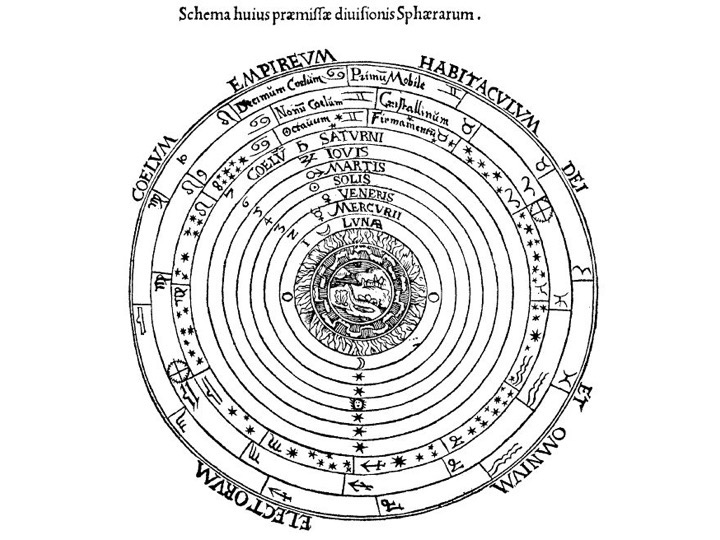
\includegraphics[width=0.5\linewidth]{img/arist} \caption{Keskaegne aristotellik maailm.}\label{fig:unnamed-chunk-2}
\end{figure}

Aristotelese suur teooria ühendab kogu maailmapildi alates meie mõistes
keemiast ja kosmoloogiast kuni bioloogia, maateaduse ja isegi
geograafiani. Sellist ühendteooriat on erakordselt raske ümber lükata,
sest seal on kõik kõigega seotud.

\begin{quote}
Aristarchus (c. 310 -- c. 230 BC) proovis seda siiski, väites, et
tegelikult tiirleb maakera ümber statsionaarse päikese. Ta uskus ka, et
kinnistähed on teised päikesed, et universum on palju suurem kui arvati
(ehkki kaasaegne seisukoht oli, et universumi mastaabis ei ole maakera
suurem kui liivatera) ning, et maakera pöörleb ümber oma telje. Paraku
ei suutnud Aristarchuse geotsentriline teooria toetajaid leida, kuna see
ei pidanud vastu vaatluslikule testile. Geotsentrilisest teooriast
tuleneb nimelt loogilise paratamatusena, et tähtedel esineb maalt
vaadates parallaks. See tähendab, et kui maakera koos astronoomiga teeb
poolringi ümber päikese, siis kinnistähe näiv asukoht taevavõlvil
muutub, sest astronoom vaatleb teda teise nurga alt. Pange oma
nimetissõrm näost u 10 cm kaugusele, sulgege parem silm, seejärel avage
see ning sulgege vasak silm ja te näete oma sõrme parallaksi selle näiva
asukoha muutusena. Mõõtmised ei näidanud aga parallaksi olemasolu (sest
maa trajektoori diameeter on palju lühem maa kaugusest tähtedest).
Parallaksi suudeti esimest korda mõõta alles 1838, siis kui juba iga
koolijüts uskus, et maakera tiirleb ümber päikese!
\end{quote}

Ühte Aristotelese kosmoloogia olulist puudust nähti siiski kohe. Nimelt
ei suuda Aristoteles seletada, miks osad planeedid teavavõlvil vahest
suunda muudavad ja mõnda aega lausa vastupidises suunas liiguvad
(retrogressioon). Kuna astronoomiat kasutasid põhiliselt astroloogid,
siis pöörati planeetide liikumisele suurt tähelepanu. Lahenduseks ei
olnud aga mitte suure teooria ümbertegemine või ümberlükkamine, vaid uue
teaduse nõudmine, mis ``päästaks fenomenid''. Siin tuli appi Ptolemaios
(c. AD 100 -- c. 170), kes lõi matemaatilise mudeli, kus planeedid mitte
lihtsalt ei liigu ringtrajektoori mõõda, vaid samal ajal teevad ka
väiksemaid ringe ümber esimese suure ringjoone. Neid väiksemaid ringe
kutsutakse epitsükliteks. See mudel suutis planeetide liikumist
taevavõlvil piisavalt hästi ennustada, et astroloogide seltskond maha
rahustada.

Ptolemaiosel ja tema järgijatel oli tegelikult mitu erinevat mudelit.
Osad neist ei sisaldanud epitsükleid ja maakera ei asunud tema mudelites
universumi keskel, vaid oli sellest punktist eemale nihutatud --- nii et
päike ei teinud ringe ümber maakera vaid ümber tühja punkti. Kuna leidus
epitsüklitega mudel ja ilma epitsükliteta mudel, mis andsid identseid
ennustusi, on selge, et Aristotelese teooria ja fenomenide päästmise
mudelid on põhimõtteliselt erinevad asjad. Samal ajal, kui Aritoteles
\textbf{seletas} maailma põhiolemust põhjuslike seoste jadana (mitte
matemaatiliselt), \textbf{kirjeldas/ennustas} Ptolemaios sellesama
maailma käitumist matemaatiliste (mitte põhjuslike) struktuuride abil.

\begin{figure}
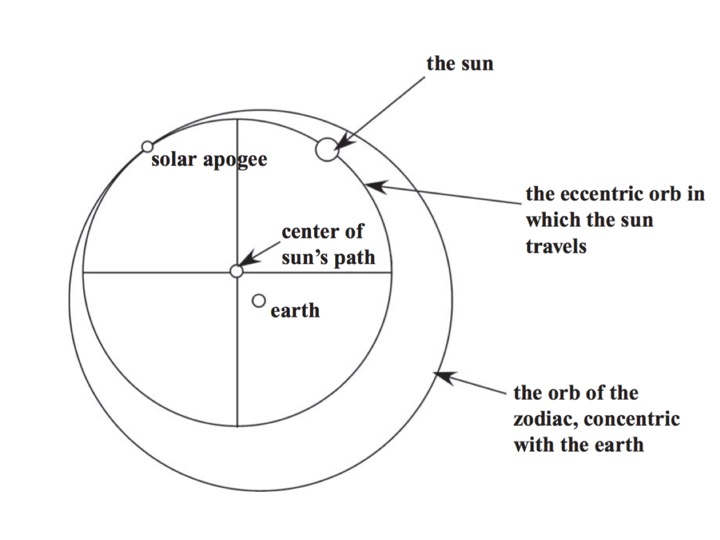
\includegraphics[width=0.5\linewidth]{img/pt2} \caption{Ilma epitsükliteta ptolemailine mudel.}\label{fig:unnamed-chunk-3}
\end{figure}

Nii tekkis olukord, kus maailma mõistmiseks kasutati Aristotelese
ühendteooriat, aga selle kirjeldamiseks ja tuleviku ennustamiseks hoopis
ptolemailisi mudeleid, mida keegi päriselt tõeks ei pidanud ja mida
hinnati selle järgi, kui hästi need ``päästsid fenomene''.

See toob meid Kopernikuse (1473 -- 1543) juurde, kes teadusajaloolaste
arvates vallandas 17. sajandi teadusliku revolutsiooni, avaldades
raamatu, kus ta asetab päikese universumi keskele ja paneb maa selle
ümber ringtrajektooril tiirlema. Kas Kopernikus tõrjus sellega kõrvale
Aristotelese, Ptolemaiose või mõlemad? Tundub, et ta soovis kolmandat,
suutis esimest ning tolleaegsete lugejate arvates üritas teha teist ---
ehk välja pakkuda alternatiivi ptolemailistele mudelitele, mis selleks
ajaks olid muutunud väga keerukaks (aga ka samavõrra ennustustäpseks).
Kuna Kopernikuse raamat läks trükki ajal, mil selle autor oli juba oma
surivoodil, kirjutas sellele eessõna üks tema vaimulikust sõber, kes
püüdis oodatavat kiriklikku pahameelt leevendada vihjates, et päikese
keskele viimine on vaid mudeldamise trikk, millest ei tasu järeldada, et
maakera ka tegelikult ümber päikese tiirleb (piibel räägib, kuidas jumal
peatas taevavõlvil päikese, mitte maa). Ja kuna eessõna oli anonüümne,
eeldasid lugejad, et selle kirjutas autor. Lisaks, kuigi Kopernikus
tõstis päikese keskele, jäi ta planeetide ringikujuliste trajektooride
juurde, mis tähendab, et selleks, et tema teooria fenomenide päästmisel
hätta ei jääks, oli ta sunnitud maad ja planeete mõõda epitsükleid ümber
päikese liigutama. Kokkuvõttes oli Kopernikuse mudel umbes sama
keeruline kui ptolemailikud mudelid ja selle abil tehtud ennustused
planeetide liikumise kohta olid väiksema täpsusega. Seega, ennustava
mudelina ei olnud sel suuri eeliseid.

\begin{figure}
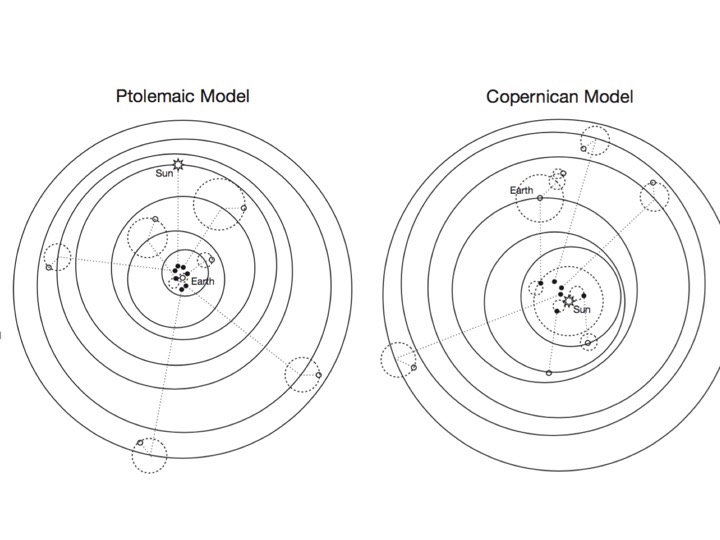
\includegraphics[width=0.5\linewidth]{img/kop} \caption{Ptolemaiose ja Kopernikuse mudelid on üllatavalt sarnased.}\label{fig:unnamed-chunk-4}
\end{figure}

\begin{quote}
Kopernikuse mudel suutis siiski ennustada mõningaid nähtusi (planeetide
näiv heledus jõuab maksimumi nende lähimas asukohas maale), mida
Ptolemaiose mudel ei ennustanud. See ei tähenda, et need fenomenid
oleksid olnud vastuolus Ptolemaiose mudeliga. Lihtsalt, nende
Ptolemaiose mudelisse sobitamiseks oli vaja osad mudeli parameetrid
fikseerida nii-öelda suvalistele väärtustele. Seega Kopernikuse mudel
töötas sellisel kujul, nagu see esitati, samas kui Ptolemaiose mudel
vajas \emph{post hoc} tuunimimst.
\end{quote}

Kui vaadata Koperniku produkti teooriana, mitte mudelina, siis oli
sellel küll selgeid eeliseid Aristotelese maailmateooria ees. Juba ammu
oli nähtud komeete üle taevavõlvi lendamas (mis Aristotelese järgi
asusid kinnistähtede muutumatus sfääris), nagu ka supernoova tekkimist
ja kadu, ning enam ei olnud kaugel aeg, mil Galileo joonistas oma
teleskoobist kraatreid kuu pinnal, näidates, et kuu ei saanud koosneda
täiuslikust viiendast elemendist ja et sellel toimusid ilmselt sarnased
füüsikalised protsessid kui maal. On usutav, et kui Kopernikus oleks
jõudnud oma raamatule ise eessõna kirjutada, oleks tema teooria
vastuvõtt olnud kiirem ja valulisem.

\chapter{Küsimused, mida statistika
küsib}\label{kusimused-mida-statistika-kusib}

Statistika abil saab vastuseid järgmisetele küsimustele:

\begin{enumerate}
\def\labelenumi{\arabic{enumi})}
\item
  kuidas näevad välja teie andmed ehk milline on just teie andmete
  jaotus, keskväärtus, varieeruvus ja koos-varieeruvus? Näiteks,
  mõõdetud pikkuste ja kaalude koos-varieeruvust saab mõõta
  korrelatsioonikordaja abil.
\item
  mida me peaksime teie andmete põhjal uskuma selle kohta, mis on
  päriselt? Näiteks, kui meie andmete põhjal arvutatud keskmine pikkus
  on 178 cm, siis kui palju on meil põhjust arvata, et tegelik
  populatsiooni keskmine pikkus \textgreater{} 185 cm?
\item
  mida ütleb statistilise mudeli struktuur teadusliku hüpoteesi kohta?
  Näiteks, kui meie poolt mõõdetud pikkuste ja kaalude koos-varieeruvust
  saab hästi kirjeldada kindlat tüüpi lineaarse regressioonimudeliga,
  siis on meil ehk tõendusmaterjali, et pikkus ja kaal on omavahel
  sellisel viisil seotud ja eelistatud peaks olema teaduslik teooria,
  mis just sellise seose tekkimisele bioloogilise mehhanismi annab.
\item
  mida ennustab mudel tuleviku kohta? Näiteks, meie lineaarne
  pikkuse-kaalu mudel suudab ennustada tulevikus kogutavaid pikkuse
  andmeid. Aga kui hästi?
\end{enumerate}

\begin{quote}
statistika peamine ülesanne on kvantifitseerida kõhedust, mida peaksime
tundma vastates eeltoodud küsimustele.
\end{quote}

Statistika ei vasta otse teaduslikele küsimustele ega küsimustele päris
maailma kohta. Statistilised vastused jäävad alati kasutatud andmete ja
mudelite piiridesse. Sellega seoses peaksime eelistama hästi kogutud
rikkalikke andmeid ja paindlikke mudeleid. Siis on lootust, et hüpe
mudeli koefitsientidest päris maailma kirjeldamisse tuleb üle kitsama
kuristiku. Bayesil on siin eelis, sest osav statistik suudab koostöös
teadlastega priori mudelisse piisavalt kasulikku infot koguda. Ühtlasi,
mida paindlikum meetod, seda vähem automaatne on selle mõistlik
kasutamine.

\section*{Jäta meelde}\label{jata-meelde}
\addcontentsline{toc}{section}{Jäta meelde}

\begin{enumerate}
\def\labelenumi{\arabic{enumi}.}
\item
  Statistika jagatakse kolme ossa: kirjeldav (summary), uuriv
  (exploratory) ja järeldav (inferential).
\item
  Kirjeldav statistika kirjeldab teie andmeid summaarsete statistikute
  abil.
\item
  Uuriv statistika püstitab valimi põhjal uusi teaduslikke hüpoteese,
  kasutades selleks põhiliselt graafilisi meetodeid.
\item
  Järeldav statistika kasutab formaalseid mudeleid, et kontrollida
  uuriva statistika abil püsitatud hüpoteese. Järeldav statistika teeb
  valimi põhjal järeldusi statistilise populatsiooni kohta, millest see
  valim pärineb.
\item
  Statistika põhjal tehtud järeldused on alati ebakindlad; ka siis kui
  need esitatakse punkthinnanguna parameetriväärtusele. Nii
  punkthinnangud kui intervall-hinnangud on lihtsustused: tegelik
  ebakindluse määr on n-dimensionaalne tõenäosuspilv, kus n on mudeli
  parameetrite arv.
\item
  Statistika põhiline ülesanne on kvantifitseerida ebakindlust, mis
  ümbritseb järeldava statistika abil saadud hinnanguid. Selle
  ebakindluse numbriline mõõt on tõenäosus, mis jääb 0 ja 1 vahele.
\item
  Tõenäosus omistab numbrilise väärtuse sellele, kui palju me usuksime
  hüpoteesi x kehtimisse, juhul kui me usuksime, et selle tõenäosuse
  arvutamiseks kasutatud statistilised mudelid vastavad tegelikkusele.
\item
  Ükski statistiline mudel ei vasta tegelikkusele ja mudelivaba
  statistikat ei ole olemas.
\end{enumerate}

\chapter{Kuidas näevad välja teie
andmed}\label{kuidas-naevad-valja-teie-andmed}

\section*{Summaarsed statistikud}\label{summaarsed-statistikud}
\addcontentsline{toc}{section}{Summaarsed statistikud}

Summaarne statistik püüab iseloomustada teie valimit ühe numbri abil.\\
Milliseid summaarseid statistikuid arvutada ja milliseid vältida, sõltub
statistilisest mudelist, mis omakorda sõltub teie andmetest ja teie
uskumustest andmeid genereeriva protsessi kohta.

Summaarse statistika abil iseloomustame

\begin{itemize}
\tightlist
\item
  tüüpilist valimi liiget (keskmise näitajad),
\item
  muutuja sisest varieeruvust (standardhälve, mad jms),
\item
  erinevate muutujate koos-varieeruvust (korrelatsioonikordaja)
\end{itemize}

\section*{Keskväärtused}\label{keskvaartused}
\addcontentsline{toc}{section}{Keskväärtused}

Keskväärtust saab mõõta paaril tosinal erineval viisil, millest
järgnevalt vaatleme kolme või nelja. Enne kui arvutama kukute, mõelge
järele, miks te soovite keskväärtust teada. Kas teid huvitab valimi
tüüpiline liige? Kuidas te sooviksite seda tüüpilisust defineerida? Kas
valimi keskmise liikmena või valimi kõige arvukama liikmena? või veel
kuidagi? See, millist keskväärtust kasutada, sõltub sageli andmejaotuse
kujust. Sümmeetrilisi jaotusi on lihtsam iseloomustada ja mitmetipulised
jaotused on selles osas kõige kehvemad.

Järgnevad nõuanded on rangelt soovituslikud:

\begin{enumerate}
\def\labelenumi{(\arabic{enumi})}
\item
  Kui valim on normaaljaotusega (histogramm on sümmeetriline), hinda
  tüüpilist liiget läbi aritmeetilise keskmise (mean).
\item
  Muidu kasuta mediaani (median). Kui valim on liiga väike, et jaotust
  hinnata (aga \textgreater{} 4), eelista mediaani. Mediaani saamiseks
  järjestatakse mõõdetud väärtused suuruse järgi ja võetakse selle rea
  keskmine liige. Mediaan on vähem tundlik ekstreemsete väärtuste
  (outlierite) suhtes kui mean.
\item
  Valimi kõige levinumat esindajat iseloomustab mood ehk jaotuse tipp.
  Seda on aga raskem täpselt määrata ja mitmetipulisel jaotusel on mitu
  moodi. Töötamisel posterioorsete jaotustega on mood sageli parim
  lahendus.
\end{enumerate}






\begin{figure}
\centering
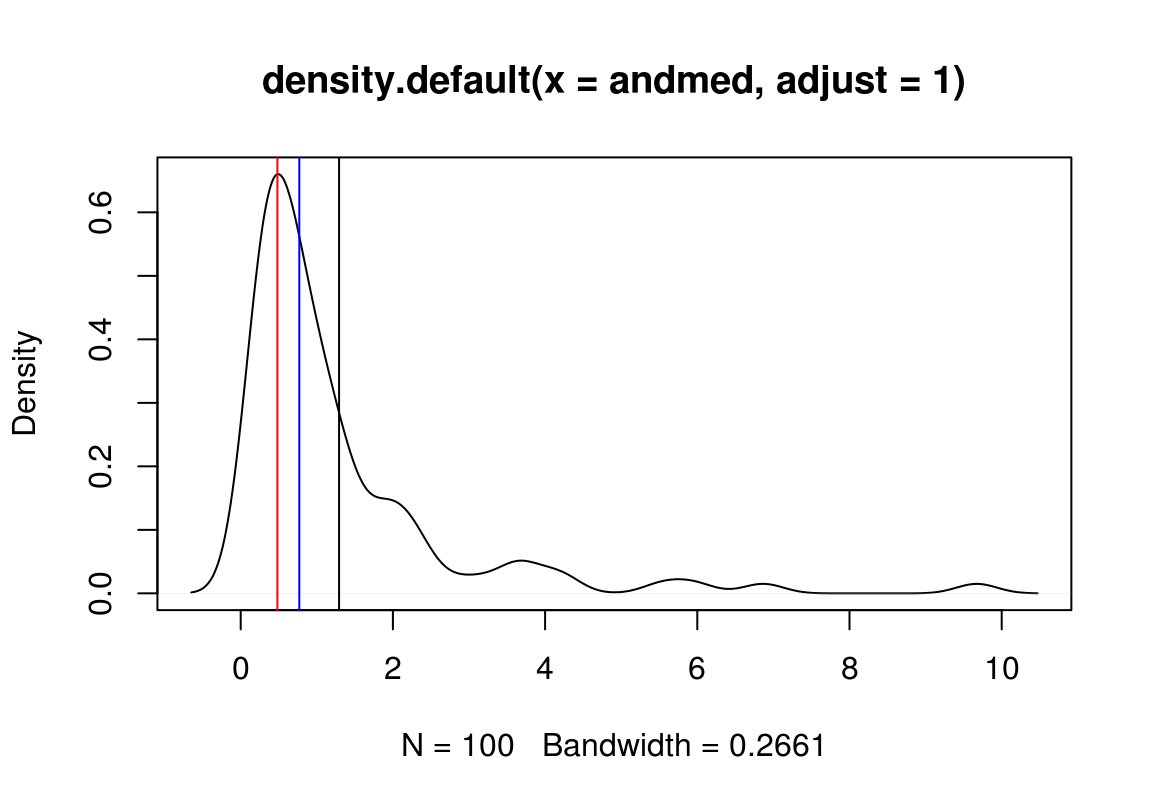
\includegraphics{03_andmed_files/figure-latex/lognorm-1.pdf}
\caption{\label{fig:lognorm}Simuleeritud lognormaaljaotusega andmed. Punane joon -
mood; sinine joon - mediaan; must joon - aritmeetiline keskmine (mean).
Milline neist vastab parimini teie intuitsiooniga nende andmete
``keskväärtusest''? Miks?}
\end{figure}

\section*{Muutuja sisene varieeruvus}\label{muutuja-sisene-varieeruvus}
\addcontentsline{toc}{section}{Muutuja sisene varieeruvus}

Aritmeetilise keskmisega (\emph{mean}) käib kokku standardhälve (SD). SD
on sama ühikuga, mis andmed (ja andmete keskväärtus). Suhtelist
standardhälvet kutsutakse variatsiooni koefitsiendiks (\emph{Coefficient
of Variation}) ja arvutatakse nii: \texttt{CV\ =\ sd(x)/mean(x)}. CV x
100\% annab varieeruvuse protsendina keskväärtusest.

Statistikute hulgas eelistatud andmete avaldamise formaat on mean (SD),
mitte mean (+/- SD). 1 SD katab 68\% normaaljaotusest, 2 SD -- 96\% ja 3
SD -- 99\%. Normaaljaotus langeb servades kiiresti, mis tähendab, et tal
on peenikesed sabad ja näiteks 5 SD kaugusel keskmisest paikneb vaid üks
punkt miljonist. Näiteks: inimeste IQ on normaaljaotusega, mean = 100,
sd = 15. See tähendab, et kui sinu IQ = 115 (mis on enam-vähem ülikooli
astujate keskmine IQ), siis on tõenäosus, et juhuslikult kohatud inimene
on sinust nutikam, 18\% ((100\% - 68\%) / 2 = 18\%).

Kui aga ``tegelikul'' andmejaotusel on ``paks saba'' (nagu eelmisel
joonisel kujutatud andmetel) või esinevad outlierid, siis normaaljaotust
eeldav mudel tagab ülehinnatud SD ja seega ülehinnatud varieeruvuse. Kui
andmed saavad olla ainult positiivsed, siis SD \textgreater{} mean/2
viitab, et andmed ei sobi normaaljaotuse mudeliga (sest mudel ennustab
negatiivsete andmete esinemist küllalt suure sagedusega).

Standardhälve on defineeritud ka mõnede teiste jaotuste jaoks peale
normaaljaotuse (Poissioni jaotus, binoomjaotus). Funktsioon sd() ja
selle taga olev võrrand sd = sqrt((mean(x) - x)\^{}2/(n - 1)) on loodud
normaaljaotuse tarbeks ja neid alternatiivseid standardhälbeid ei
arvuta. Veelgi enam, igale jaotusele, mida me oskame integreerida, saab
ka integraali abil õige katvusega standardhälbe arvutada. Seega tasub
meeles pidada, et tavapärane viis standardhälbe arvutamiseks sd() abil
kehtib normaaljaotuse mudeli piirides ja ei kusagil mujal! Siiski, kui
arvutada standardhälbe sd()-ga, võib olla kindel, et jaotusest sõltumata
hõlvavad 2 SD-d vähemalt 75\% andmejaotusest. Kui andmed ei sobi
normaaljaotusesse ja te ei ole rahul tulemusega, mille tõlgendus on
niivõrd ebakindel kui 75 protsenti kuni 96+ protsenti, võib pakkuda
kahte alternatiivset lahendust:

\section*{Logaritmi andmed}\label{logaritmi-andmed}
\addcontentsline{toc}{section}{Logaritmi andmed}

Kui kõik andmeväärtused on positiivsed ja andmed on lognormaaljaotusega,
siis logaritmimine muudab andmed normaalseks. Logaritmitud andmetest
tuleks arvutada aritmeetiline keskmine ja SD ning seejärel mõlemad
anti-logaritmida (näiteks, kui log2(10) = 3.32, siis antilogaritm
sellest on 2\^{}3.32 = 10). Sellisel juhul avaldatakse lõpuks
geomeetriline keskmine ja multiplikatiivne SD algses lineaarses skaalas
(multiplikatiivne SD = geom mean x SD; geom mean/SD). Geomeetriline
keskmine on alati väiksem kui aritmeetiline keskmine. Lisaks on SD
intervall nüüd asümmeetriline ja SD on alati \textgreater{} 0. See
protseduur tagab, et 68\% lognormaalsetest andmetest jääb 1 SD vahemikku
ning 96\% andmetest jääb 2 SD vahemikku.

Kui lognormaalsetele andmetele arvutada tavaline SD lineaarses skaalas
kasutades sd() funktsiooni, siis tuleb SD sageli palju laiem kui peaks
ja hõlmab ka negatiivseid väärtusi (pea meeles, et SD definitsiooni
järgi jääb 96\% populatsioonist 2 SD vahemikku).\\
Sageli on aga negatiivsed muutuja väärtused võimatud (näiteks nädalas
suitsetatud sigarettide arv).

Logaritmimise kaudu avaldatud multiplikatsiivse SD arvutamiseks kasutame
enda kirjutatud funktsiooni mulitplicative\_sd(). Esiteks arvutame
multiplikatiivse ja aditiivse sd lognormaalsetele andmetele, mida
kujutasime eelmisel joonisel:

\begin{Shaded}
\begin{Highlighting}[]
\NormalTok{multiplicative_sd <-}\StringTok{ }\ControlFlowTok{function}\NormalTok{(x) \{}
\NormalTok{  x <-}\StringTok{ }\KeywordTok{na.omit}\NormalTok{(x) }\CommentTok{#viskan välja NA-d (kui neid on)}
\NormalTok{  log_data <-}\StringTok{ }\KeywordTok{log10}\NormalTok{(x) }\CommentTok{#logaritmin andmed}
\NormalTok{  log_mean <-}\StringTok{ }\KeywordTok{mean}\NormalTok{(log_data) }\CommentTok{#keskmine logaritmitud andmetest}
\NormalTok{  log_sd <-}\StringTok{ }\KeywordTok{sd}\NormalTok{(log_data) }\CommentTok{#SD logaritmitud andmetest}
\NormalTok{  geom_mean <-}\StringTok{ }\DecValTok{10}\OperatorTok{^}\NormalTok{log_mean }\CommentTok{#anti-logaritm annab geomeetrilise keskmise}
\NormalTok{  mult_sd <-}\StringTok{ }\DecValTok{10}\OperatorTok{^}\NormalTok{log_sd }\CommentTok{#anti-logaritm annab multiplikatiivse SD}
\NormalTok{  lower1 <-}\StringTok{ }\NormalTok{geom_mean}\OperatorTok{/}\NormalTok{mult_sd }\CommentTok{#alumine SD piir}
\NormalTok{  upper1 <-}\StringTok{ }\NormalTok{geom_mean }\OperatorTok{*}\StringTok{ }\NormalTok{mult_sd }\CommentTok{#ülemine SD piir}
\NormalTok{  lower2 <-}\StringTok{ }\NormalTok{geom_mean}\OperatorTok{/}\NormalTok{(mult_sd}\OperatorTok{^}\DecValTok{2}\NormalTok{) }\CommentTok{#alumine 2 SD piir}
\NormalTok{  upper2 <-}\StringTok{ }\NormalTok{geom_mean }\OperatorTok{*}\StringTok{ }\NormalTok{(mult_sd}\OperatorTok{^}\DecValTok{2}\NormalTok{) }\CommentTok{#ülemine 2 SD piir}
\NormalTok{  Mean <-}\StringTok{ }\KeywordTok{mean}\NormalTok{(x) }\CommentTok{#aritmeetiline keskmine}
\NormalTok{  lower3 <-}\StringTok{ }\KeywordTok{mean}\NormalTok{(x) }\OperatorTok{-}\StringTok{ }\KeywordTok{sd}\NormalTok{(x) }\CommentTok{#alumine additiivse SD piir}
\NormalTok{  upper3 <-}\StringTok{ }\KeywordTok{mean}\NormalTok{(x) }\OperatorTok{+}\StringTok{ }\KeywordTok{sd}\NormalTok{(x) }\CommentTok{#ülemine additiivse SD piir}
\NormalTok{  lower4 <-}\StringTok{ }\KeywordTok{mean}\NormalTok{(x) }\OperatorTok{-}\StringTok{ }\KeywordTok{sd}\NormalTok{(x)}\OperatorTok{*}\DecValTok{2} \CommentTok{#alumine additiivse 2 SD piir}
\NormalTok{  upper4 <-}\StringTok{ }\KeywordTok{mean}\NormalTok{(x) }\OperatorTok{+}\StringTok{ }\KeywordTok{sd}\NormalTok{(x)}\OperatorTok{*}\DecValTok{2} \CommentTok{#ülemine additiivse 2 SD piir}
  \KeywordTok{tibble}\NormalTok{(}\DataTypeTok{SD =} \KeywordTok{c}\NormalTok{(}\StringTok{"multiplicative_SD"}\NormalTok{, }
                \StringTok{"multiplicative_2_SD"}\NormalTok{, }
                \StringTok{"additive_SD"}\NormalTok{, }
                \StringTok{"additive_2_SD"}\NormalTok{), }
         \DataTypeTok{MEAN =} \KeywordTok{c}\NormalTok{(geom_mean, }
\NormalTok{                  geom_mean, }
\NormalTok{                  Mean, }
\NormalTok{                  Mean), }
         \DataTypeTok{lower =} \KeywordTok{c}\NormalTok{(lower1, }
\NormalTok{                   lower2, }
\NormalTok{                   lower3, }
\NormalTok{                   lower4), }
         \DataTypeTok{upper =} \KeywordTok{c}\NormalTok{(upper1, }
\NormalTok{                   upper2, }
\NormalTok{                   upper3, }
\NormalTok{                   upper4))}
\NormalTok{\}}
\NormalTok{andmed <-}\StringTok{ }\KeywordTok{rlnorm}\NormalTok{(}\DecValTok{100}\NormalTok{) }\CommentTok{#100 juhuslikku arvu lognormaaljaotusest}
\KeywordTok{multiplicative_sd}\NormalTok{(andmed) }\OperatorTok\StringTok{ }\NormalTok{knitr}\OperatorTok{::}\KeywordTok{kable}\NormalTok{()}
\end{Highlighting}
\end{Shaded}

\begin{tabular}{l|r|r|r}
\hline
SD & MEAN & lower & upper\\
\hline
multiplicative\_SD & 0.939 & 0.375 & 2.36\\
\hline
multiplicative\_2\_SD & 0.939 & 0.149 & 5.91\\
\hline
additive\_SD & 1.448 & -0.146 & 3.04\\
\hline
additive\_2\_SD & 1.448 & -1.740 & 4.64\\
\hline
\end{tabular}

Tavalise aritmeetitilise keskmise asemel on meil nüüd geomeetriline
keskmine. Võrdluseks on antud ka tavaline (aritmeetiline) keskmine ja
(aditiivne) SD. Additiivne SD on selle jaotuse kirjeldamiseks selgelt
ebaadekvaatne (vt jaotuse pilti ülalpool ja võrdle mulitplikatiivse
SD-ga).

Kuidas aga töötab multiplikatiivne standardhälve normaaljaotusest pärit
andmetega (N=3, mean=100, sd=20)? Kui multiplikatiivse sd rakendamine
normaalsete andmete peal viiks katastroofini, siis poleks sel
statistikul suurt kasutusruumi.

\begin{tabular}{l|r|r|r}
\hline
SD & MEAN & lower & upper\\
\hline
multiplicative\_SD & 108 & 92.8 & 126\\
\hline
multiplicative\_2\_SD & 108 & 79.7 & 147\\
\hline
additive\_SD & 109 & 92.1 & 126\\
\hline
additive\_2\_SD & 109 & 75.2 & 143\\
\hline
\end{tabular}

Nagu näha, on multiplikatiivse sd kasutamine normaalsete andmetega pigem
ohutu (kui andmed on positiivsed). Arvestades, et additiivne SD on
lognormaalsete andmete korral kõike muud kui ohutu ning et
lognormaaljaotus on bioloogias üsna tavaline, eriti ensüümreaktsioonide
ja kasvuprotsesside juures, on mõistlik alati kasutada
multiplicative\_sd() funktsiooni. Kui mõlema SD väärtused on sarnased,
siis võib loota, et andmed on normaalsed ning saab refereede rõõmuks
avaldada tavapärase additiivse SD.

\begin{quote}
kui n \textless{} 10, siis mõlemad SD-d alahindavad süstemaatiliselt
tegelikku sd-d. Ettevaatust väikeste valimitega!
\end{quote}

Vahest tekkib teil vajadus empiiriliselt määrata, kas teie andmed on
normaaljaotusega. Enne kui seda tegema asute, peaksite mõistma, et see,
et teie valim ei ole normaalne, ei tähenda automaatselt, et
populatsioon, millest see valim tõmmati, ei oleks normaaljaotusega. Igal
juhul, valimiandmete normaalsuse määramiseks on kõige mõistlikum
kasutada qq-plotti. QQ-plot (kvantiil-kvantiil plot) võrdleb andmete
jaotust ideaalse normaaljaotusega andmepunkti haaval. Kui empiiriline
jaotus kattub referentsjaotusega, siis on tulemuseks sirgel paiknevad
punktid. Järgneval qq plotil on näha, mis juhtub, kui plottida
lognormaalseid andmeid normaaljaotuse vastu:








\begin{Shaded}
\begin{Highlighting}[]
\KeywordTok{qqPlot}\NormalTok{(andmed)}
\end{Highlighting}
\end{Shaded}

\begin{figure}
\centering
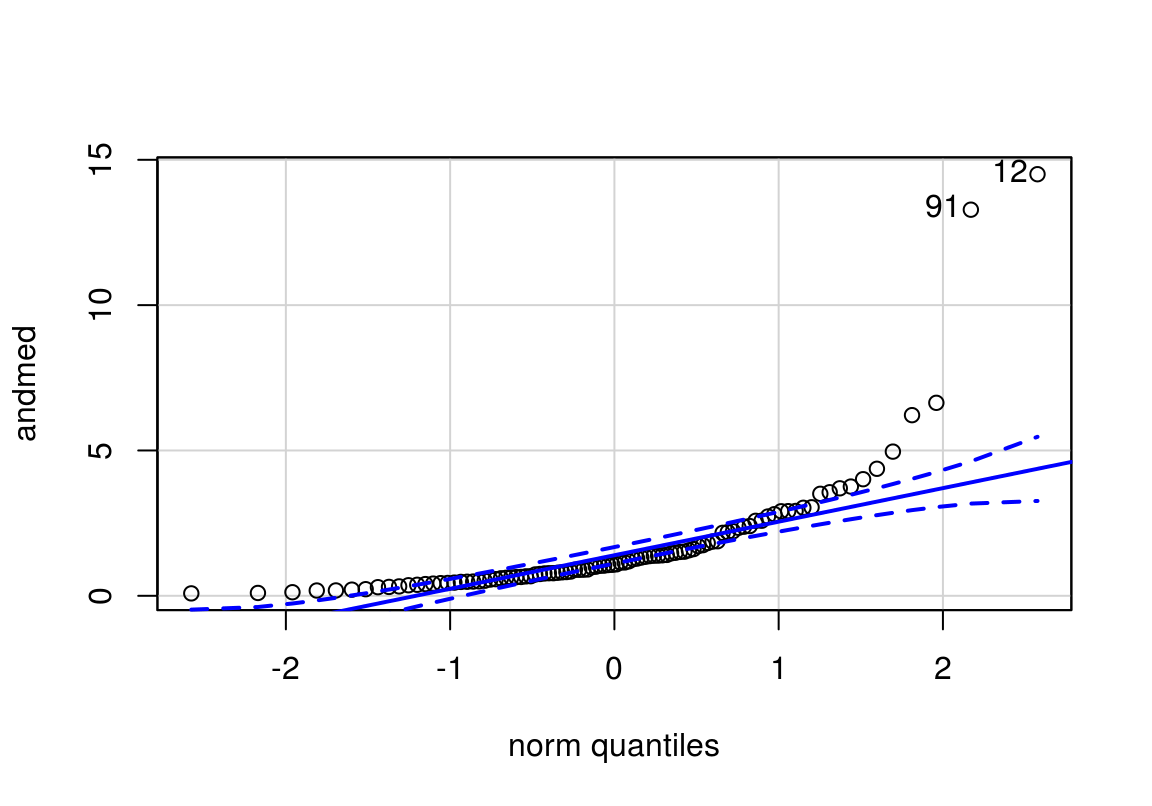
\includegraphics{03_andmed_files/figure-latex/qqnorm-1.pdf}
\caption{\label{fig:qqnorm}QQ-plot lognormaalsetele andmetele. Plotil võrreldakse
lognormaalsete andmete jaotust referentsjaotusega, milleks on antud
juhul normaaljaotus. Punased katkendjooned annavad standardveapõhise
usaldusvahemiku (arvutatud simuleeritud juhuvalimist normaaljaotusega
referentspopulatsioonist), millesse peaks jääma enamus andmepunkte juhul
kui andmepunktid pärineksid normaaljaotusest.}
\end{figure}

\begin{verbatim}
#> [1] 66 65
\end{verbatim}

Nüüd joonistame qq-ploti logaritmitud andmetele.




\begin{Shaded}
\begin{Highlighting}[]
\KeywordTok{qqPlot}\NormalTok{(}\KeywordTok{log}\NormalTok{(andmed))}
\end{Highlighting}
\end{Shaded}

\begin{figure}
\centering
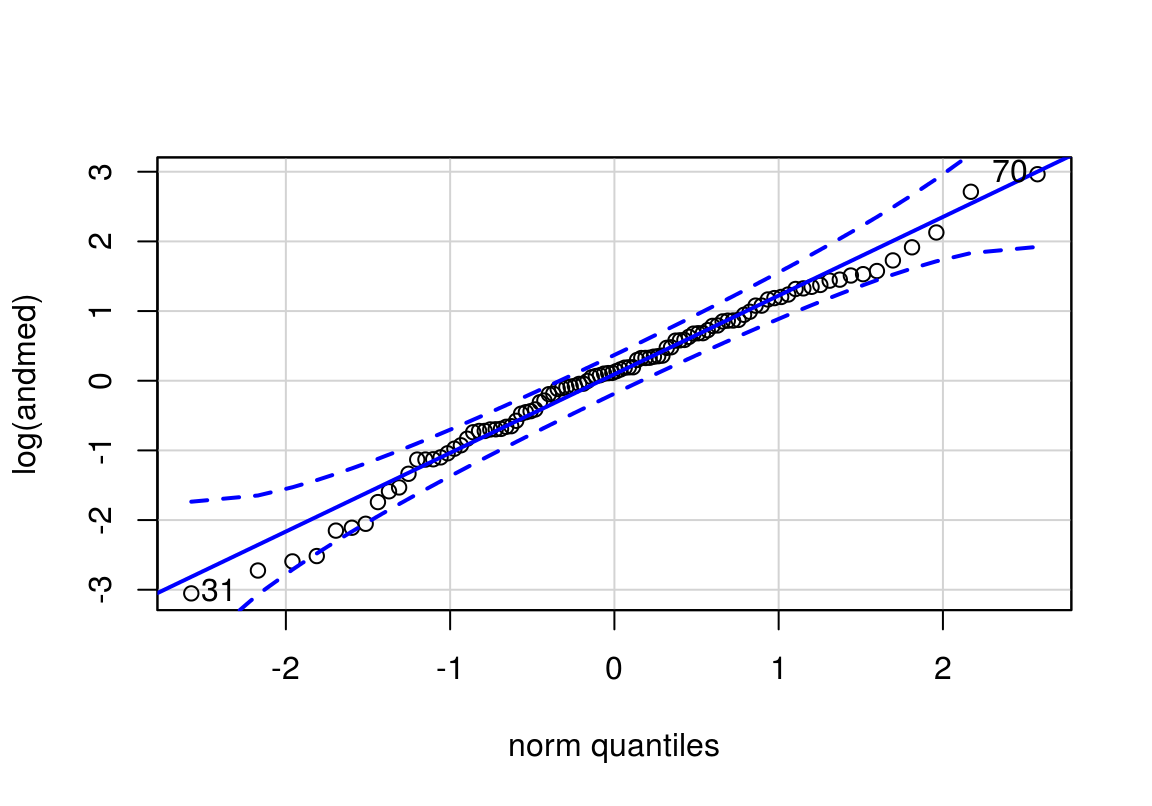
\includegraphics{03_andmed_files/figure-latex/qqlognorm-1.pdf}
\caption{\label{fig:qqlognorm}QQ-plot normaalsetele andmetele (logaritmitud
lognormaalsed andmed).}
\end{figure}

\begin{verbatim}
#> [1] 66 65
\end{verbatim}

Pole kahtlust, andmed on logaritmitud kujul normaaljaotusega.

\begin{quote}
qqPlot() võimaldab võrrelda teie andmeid ükskõik millise R-is
defineeritud jaotusega (?car::qqPlot).
\end{quote}

Normaaljaotuse kindlakstegemiseks on loodud ka peotäis sageduslikke
teste, mis annavad väljundina p väärtuse. Nende kasutamisest soovitame
siiski hoiduda, sest tulemused on sageli ebakindlad, eriti väikestel ja
suurtel valimitel. Mõistlikum on vaadata kõikide andmepunktide plotti
normaaljaotuse vastu, kui jõllitada ühte numbrit (p), mille väärtus,
muuseas, monotooniliselt langeb koos valimi suuruse kasvuga.

\section*{Iseloomusta andmeid algses skaalas: mediaan
(MAD)}\label{iseloomusta-andmeid-algses-skaalas-mediaan-mad}
\addcontentsline{toc}{section}{Iseloomusta andmeid algses skaalas:
mediaan (MAD)}

MAD ---- median absolute deviation --- on vähem tundlik outlierite
suhtes ja ei eelda normaaljaotust. Puuduseks on, et MAD ei oma
tõlgendust, mille kohaselt ta hõlmaks kindlat protsenti populatsiooni
või valimi andmejaotusest. Seevastu sd puhul võime olla kindlad, et
isegi kõige hullema jaotuse korral jäävad vähemalt 75\% andmetest 2 SD
piiridesse.

Lognormaalsete andmetega:

\begin{Shaded}
\begin{Highlighting}[]
\KeywordTok{mad}\NormalTok{(andmed, }\DataTypeTok{constant =} \DecValTok{1}\NormalTok{); }\KeywordTok{sd}\NormalTok{(andmed); }\KeywordTok{mad}\NormalTok{(andmed)}
\CommentTok{#> [1] 0.522}
\CommentTok{#> [1] 1.59}
\CommentTok{#> [1] 0.774}
\end{Highlighting}
\end{Shaded}

\begin{Shaded}
\begin{Highlighting}[]
\KeywordTok{mad}\NormalTok{(}\KeywordTok{log10}\NormalTok{(andmed), }\DataTypeTok{constant =} \DecValTok{1}\NormalTok{); }\KeywordTok{sd}\NormalTok{(}\KeywordTok{log10}\NormalTok{(andmed)); }\KeywordTok{mad}\NormalTok{(}\KeywordTok{log10}\NormalTok{(andmed))}
\CommentTok{#> [1] 0.275}
\CommentTok{#> [1] 0.399}
\CommentTok{#> [1] 0.408}
\end{Highlighting}
\end{Shaded}

mad = median(abs(median(x) - x)), mida on väga lihtne mõista. Samas R-i
funktsioon mad() korrutab default-ina mad-i läbi konstandiga 1.4826, mis
muudab mad()-i tulemuse võrreldavaks sd-ga, tehes sellest sd robustse
analoogi. Robustse sellepärast, et mad-i arvutuskäik, mis sõltub
mediaanist, mitte aritmeetilisest keskmisest, ei ole tundlik outlierite
suhtes. Seega, kui tahate arvutada mad-i, siis fikseerige mad()
funktsioonis argument \emph{constant} ühele.

\begin{quote}
Ära kunagi avalda andmeid vormis: mean (MAD) või median (SD). Korrektne
vorm on mean (SD) või median (MAD).
\end{quote}

Veel üks viis andmejaotuse summeerimiseks on kasutada kvantiile. Siin
saame me tüüpiliselt rohkem kui ühe numbri, aga sageli on selline viis
informatiivsem, kui ühenumbrilised summaarsed statistikud. Funktsioon
quantile võimaldab valida, milliseid kvantiile soovite näha. Järgnevas
koodist saame teada, millisest vektori ``andmed'' väärtusest allapoole
jääb 2.5\%, 25\%, 50\%, 75\% ja 95\% väärtusi.

\begin{Shaded}
\begin{Highlighting}[]
\KeywordTok{quantile}\NormalTok{(andmed, }\KeywordTok{c}\NormalTok{(}\FloatTok{0.025}\NormalTok{, }\FloatTok{0.25}\NormalTok{, }\FloatTok{0.5}\NormalTok{, }\FloatTok{0.75}\NormalTok{, }\FloatTok{0.95}\NormalTok{))}
\CommentTok{#>  2.5%   25%   50%   75%   95% }
\CommentTok{#> 0.194 0.471 0.935 1.634 4.488}
\end{Highlighting}
\end{Shaded}

\section*{Muutujate koosvarieeruvus}\label{muutujate-koosvarieeruvus}
\addcontentsline{toc}{section}{Muutujate koosvarieeruvus}

Andmete koos-varieeruvust mõõdetakse korrelatsiooni abil. Tulemuseks on
üks number - korrelatsioonikordaja r, mis varieerub -1 ja 1 vahel.

\begin{itemize}
\tightlist
\item
  r = 0 -- kahte tüüpi mõõtmised (x=pikkus, y=kaal) samadest
  mõõteobjektidest varieeruvad üksteisest sõltumatult.
\item
  r = 1: kui ühe muutuja väärtus kasvab, kasvab ka teise muutuja väärtus
  alati täpselt samas proportsioonis.
\item
  r = -1: kui ühe muutuja väärtus kasvab, kahaneb teise muutuja väärtus
  alati täpselt samas proportsioonis.
\end{itemize}

Kui r on -1 või 1, saame me x väärtust teades täpselt ennustada y
väärtuse (ja vastupidi, teades y väärrust saame täpselt ennustada x
väärtuse).\\
Kuidas tõlgendame aga tulemust \(r = 0.9\)? Mitte kuidagi. Selle asemel
tõlgendame \(r^2 = 0.9^2 = 0.81\) -- mis tähendab, et x-i varieeruvus
suudab seletada mitte rohkem kui 81\% y varieeruvusest ja vastupidi, et
Y-i varieeruvus suudab seletada 81\% X-i varieeruvusest.

Korrelatsiooni saab mõõta mitmel viisil (\texttt{?cor.test,\ method=}).
Kõige levinum on Pearsoni korrelatsioonikoefitsient, mis eeldab,
\emph{(i)} et me mõõdame pidevaid muutujaid, \emph{(ii)} juhuvalimit,
\emph{(iii)} et populatsiooniandmed on normaaljaotusega ja \emph{(iv)}
et igal mõõteobjektil on mõõdetud 2 omadust (pikkus ja kaal, näiteks).
Tuntuim alternatiiv on mitteparameetriline Spearmani korrelatsioon, mis
ei eelda andmete normaaljaotust ega seda, et mõõdetakse pidevaid
suurusi. Kui Pearsoni korrelatsiooni eeldused on täidetud ja te kasutate
siiski Spearmani korrelatsiooni, siis langeb teie arvutuse efektiivsus
ca. 10\% võrra.

\begin{Shaded}
\begin{Highlighting}[]
\KeywordTok{cor}\NormalTok{(iris}\OperatorTok{$}\NormalTok{Sepal.Length, iris}\OperatorTok{$}\NormalTok{Sepal.Width, }\DataTypeTok{use =} \StringTok{"complete.obs"}\NormalTok{)}
\CommentTok{#> [1] -0.118}
\end{Highlighting}
\end{Shaded}

Korrelatsioonikordaja väärtus sõltub mitte ainult andmete
koosvarieeruvusest vaid ka andmete ulatusest. Suurema ulatusega andmed X
ja/või Y teljel annavad keskeltläbi 0-st kaugemal oleva
korrelatsioonikordaja. Selle pärast sobib korrelatsioon halvasti näiteks
korduskatsete kooskõla mõõtmiseks.

Lisaks, korrelatsioonikordaja mõõdab vaid andmete \emph{lineaarset}
koos-varieeruvust: kui andmed koos-varieeruvad mitte-lineaarselt, siis
võivad ka väga tugevad koos-varieeruvused jääda märkamatuks.






\begin{figure}
\centering
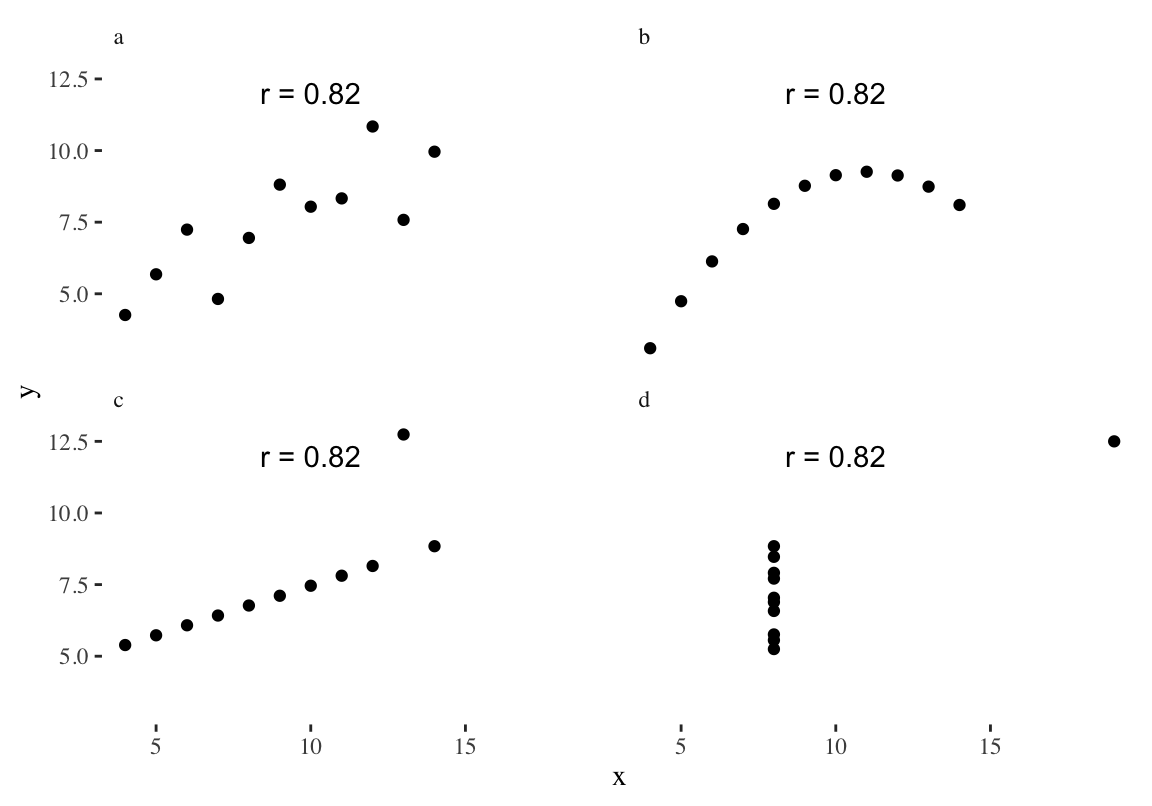
\includegraphics{03_andmed_files/figure-latex/anscombe-1.pdf}
\caption{\label{fig:anscombe}Anscombe'i kvartett illustreerib korrelatsioonikordaja
lineaarset olemust: neli andmestikku annavad identse
korrelatsioonikordaja (Pearsons'r), ehkki tegelikud seosed andmete vahel
on täiesti erinevad.}
\end{figure}

Moraal seisneb selles, et enne korrelatsioonikordaja arvutamist tasub
alati plottida andmed, et veenduda võimaliku seose lineaarsuses.
Lineaarsuse puudumine andmete koosvarieeruvuse mustris tähendab, et
korrelatsioonikordaja tuleb eksitav.

Korrelatsioonikordaja mõõdab pelgalt määra, mil üks muutuja muutub siis,
kui teine muutuja muutub. Seega ei ole suurt mõtet arvutada
korrelatsioonikordajat juhul kui me teame ette seose olemasolust kahe
muutuja vahel. Näiteks, kui sama entiteeti mõõdetakse kahel erineval
viisil, või kahes korduses, või kui esimene muutuja arvutatakse teise
muutuja kaudu.

\begin{quote}
Kõik summaarsed statistikud kaotavad suure osa teie andmetes leiduvast
infost -- see kaotus on õigustatud ainult siis, kui teie poolt valitud
statistik iseloomustab hästi andmete sügavamat olemust (näiteks
tüüpilist mõõtmistulemust või andmete varieeruvust).
\end{quote}

Korrelatsioonimaatriksi saab niimoodi:

\begin{Shaded}
\begin{Highlighting}[]
\CommentTok{# numeric columns only!}
\CommentTok{# the following gives cor matrix with }
\CommentTok{# frequentist correction for mutliple testing:}
\CommentTok{# print(psych::corr.test(iris[-5]))}
\CommentTok{# only numeric cols allowed! Hence -Species}
\NormalTok{knitr}\OperatorTok{::}\KeywordTok{kable}\NormalTok{(}\KeywordTok{cor}\NormalTok{(iris[,}\OperatorTok{-}\DecValTok{5}\NormalTok{]))}
\end{Highlighting}
\end{Shaded}

\begin{tabular}{l|r|r|r|r}
\hline
  & Sepal.Length & Sepal.Width & Petal.Length & Petal.Width\\
\hline
Sepal.Length & 1.000 & -0.118 & 0.872 & 0.818\\
\hline
Sepal.Width & -0.118 & 1.000 & -0.428 & -0.366\\
\hline
Petal.Length & 0.872 & -0.428 & 1.000 & 0.963\\
\hline
Petal.Width & 0.818 & -0.366 & 0.963 & 1.000\\
\hline
\end{tabular}

\chapter{Lineaarsed mudelid}\label{lineaarsed-mudelid}

\begin{Shaded}
\begin{Highlighting}[]
\KeywordTok{library}\NormalTok{(tidyverse)}
\KeywordTok{library}\NormalTok{(ggthemes)}
\KeywordTok{library}\NormalTok{(broom)}
\KeywordTok{library}\NormalTok{(modelr)}
\KeywordTok{library}\NormalTok{(viridis)}
\end{Highlighting}
\end{Shaded}

\section{Sirge võrrand}\label{sirge-vorrand}

Oletame, et me mõõtsime N inimese pikkuse cm-s ja kaalu kg-s ning meid
huvitab, kuidas inimeste pikkus sõltub nende kaalust. Lihtsaim mudel
pikkuse sõltuvusest kaalust on pikkus = kaal (formaliseeritult: y = x)
ja see mudel ennustab, et kui Juhani kaal = 80 kg, siis Juhan on 80 cm
pikkune. Siin on pikkus muutuja, mille väärtust ennustatakse (y) ja kaal
muutuja x, mille väärtuste põhjal ennustatakse pikkusi. Muidugi, sama
hästi võiksime ennustada kaalu pikkuste põhjal, ja kumma ennustuse
valime sõltub siinkohal eeskätt meie teaduslikest huvidest.

Veelgi enam, sama mudel ennustab, et kui Juhani kaal = 80 tonni, siis on
Juhan samuti 80 cm pikkune (eeldusel, et me avaldame x muutuja tonnides
ja y muutuja sentimeetrites). Seega, mudeli ennustuse täpsus sõltub
ühikutest, milles me andmed mudelisse sisse anname.

\begin{Shaded}
\begin{Highlighting}[]
\CommentTok{#Genereerime andmed: x = pikkus ja y = kaal:}
\NormalTok{x <-}\StringTok{ }\DecValTok{0}\OperatorTok{:}\DecValTok{100}
\NormalTok{y <-}\StringTok{ }\NormalTok{x}
\end{Highlighting}
\end{Shaded}

Selle mudeli saame graafiliselt kujutada nii:




\begin{Shaded}
\begin{Highlighting}[]
\KeywordTok{plot}\NormalTok{(y }\OperatorTok{~}\StringTok{ }\NormalTok{x, }
     \DataTypeTok{type =} \StringTok{"l"}\NormalTok{, }
     \DataTypeTok{xlab =} \StringTok{"Weight in kg"}\NormalTok{, }
     \DataTypeTok{ylab =} \StringTok{"Heigth in cm"}\NormalTok{, }
     \DataTypeTok{main =} \KeywordTok{bquote}\NormalTok{(y }\OperatorTok{==}\StringTok{ }\NormalTok{x))}
\end{Highlighting}
\end{Shaded}

\begin{figure}

{\centering 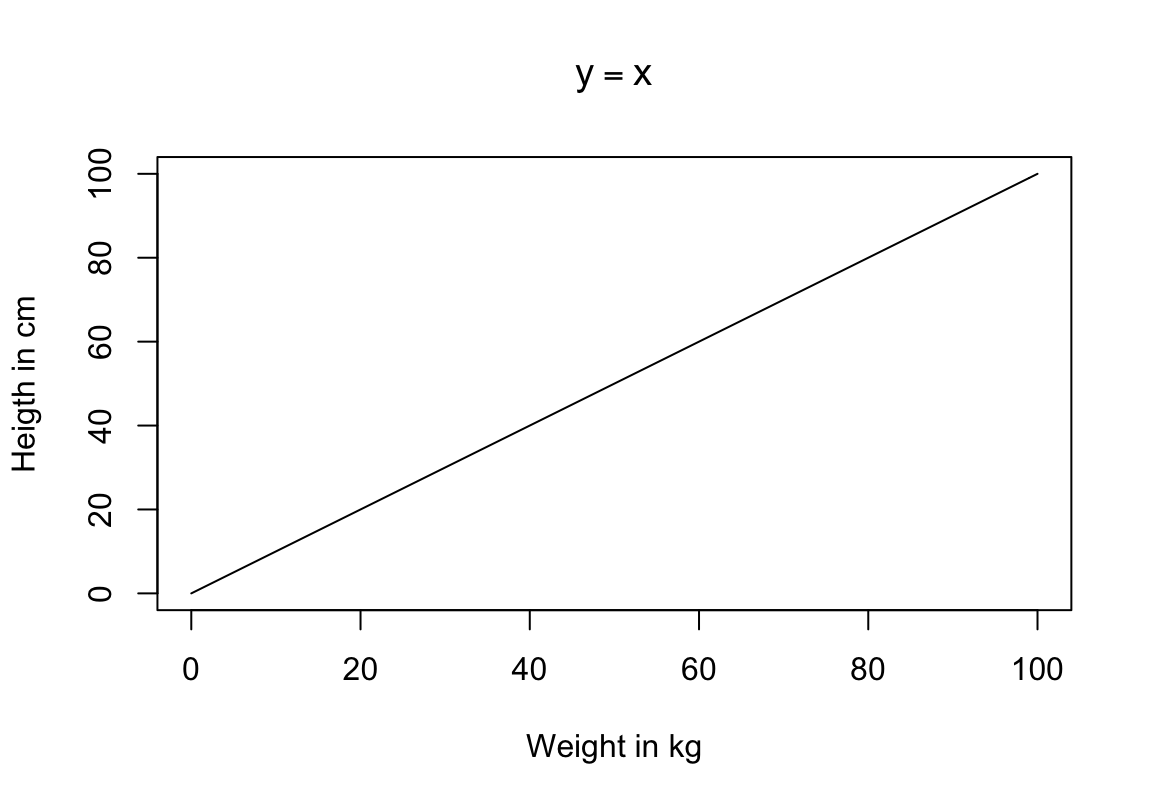
\includegraphics[width=0.7\linewidth]{04_lineaarsed_mudelid_files/figure-latex/lihtnemudel-1} 

}

\caption{Lihtne mudel y \textasciitilde{} x, mille lõikepunkt =
0 ja tõus = 1.}\label{fig:lihtnemudel}
\end{figure}

\begin{quote}
Üldistatult, mudeli keeles tähistame me seda muutujat, mille väärtusi me
ennustame, Y-ga ja seda muutujat, mille väärtuse põhjal me ennustame,
X-ga.
\end{quote}

Sirge mudeli lihtsaim matemaatiline formalism on Y = X. See on äärmiselt
jäik mudel: sirge, mille asukoht on rangelt fikseeritud. Sirge lõikab y
telge alati 0-s (mudeli keeles: sirge \emph{intercept} ehk lõikepunkt Y
teljel = 0) ja tema tõusunurk saab olla ainult 45 kraadi (mudeli keeles
\emph{slope} ehk tõus = 1). Selle mudeli jäikus tuleneb sellest, et
temas ei ole parameetreid, mille väärtusi me saaksime vabalt muuta ehk
tuunida.

Mis juhtub, kui me lisame mudelisse konstandi, mille liidame x-i
väärtustele?

\[y = a + x\]

See konstant on mudeli parameeter, mille väärtuse võime vabalt valida.
Järgnevalt anname talle väärtuse 30 (ilma konkreetse põhjuseta).

\begin{Shaded}
\begin{Highlighting}[]
\NormalTok{x <-}\StringTok{ }\DecValTok{0}\OperatorTok{:}\DecValTok{100} 
\NormalTok{a <-}\StringTok{ }\DecValTok{30}
\NormalTok{y <-}\StringTok{ }\NormalTok{a }\OperatorTok{+}\StringTok{ }\NormalTok{x}
\end{Highlighting}
\end{Shaded}




\begin{Shaded}
\begin{Highlighting}[]
\KeywordTok{plot}\NormalTok{(y }\OperatorTok{~}\StringTok{ }\NormalTok{x, }\DataTypeTok{xlim =} \KeywordTok{c}\NormalTok{(}\DecValTok{0}\NormalTok{, }\DecValTok{100}\NormalTok{), }\DataTypeTok{ylim =} \KeywordTok{c}\NormalTok{(}\DecValTok{0}\NormalTok{, }\DecValTok{150}\NormalTok{), }\DataTypeTok{type =} \StringTok{"l"}\NormalTok{,}
     \DataTypeTok{main =} \KeywordTok{bquote}\NormalTok{(y }\OperatorTok{==}\StringTok{ }\NormalTok{a }\OperatorTok{+}\StringTok{ }\NormalTok{x))}
\KeywordTok{abline}\NormalTok{(}\KeywordTok{c}\NormalTok{(}\DecValTok{0}\NormalTok{, }\DecValTok{1}\NormalTok{), }\DataTypeTok{lty =} \DecValTok{2}\NormalTok{)}
\end{Highlighting}
\end{Shaded}

\begin{figure}

{\centering 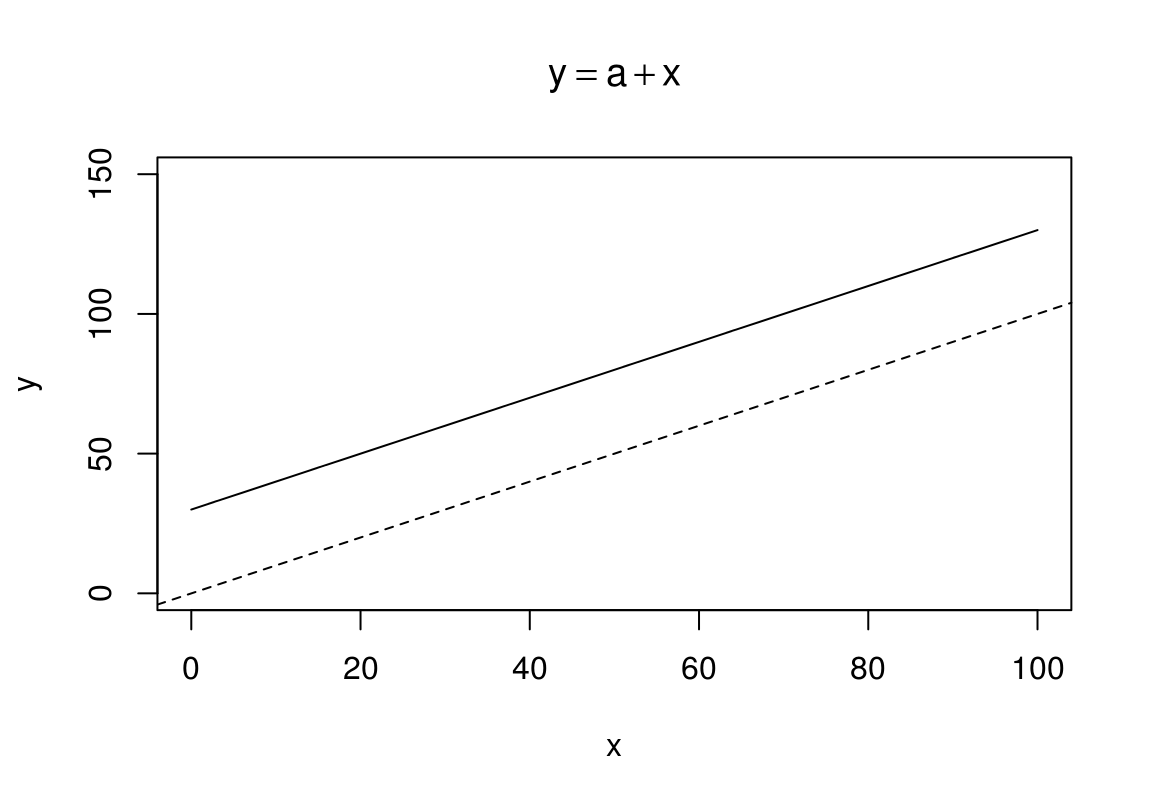
\includegraphics[width=0.7\linewidth]{04_lineaarsed_mudelid_files/figure-latex/intercept-1} 

}

\caption{Lineaarne mudel, mille lõikepunkt = 30 ja tõus = 1.
Katkendjoon, lõikepunkt = 0. Pidevjoon, lõikepunkt = 30}\label{fig:intercept}
\end{figure}

Meie konstant a määrab \(y\) väärtuse, kui \(x = 0\), ehk sirge
lõikepunkti \(y\) teljel. Teisisõnu, a = mudeli lõikepunkt
(\emph{intercept}).

Mis juhtub, kui me mitte ei liida, vaid korrutame \emph{x}-i
konstandiga?

\[y =  b \times x\]

Jällegi, me anname mudeli parameetrile b suvalise väärtuse, 3.

\begin{Shaded}
\begin{Highlighting}[]
\NormalTok{x <-}\StringTok{ }\DecValTok{0}\OperatorTok{:}\DecValTok{200}
\NormalTok{b <-}\StringTok{ }\DecValTok{3}
\NormalTok{y <-}\StringTok{ }\NormalTok{b }\OperatorTok{*}\StringTok{ }\NormalTok{x}
\end{Highlighting}
\end{Shaded}

\begin{Shaded}
\begin{Highlighting}[]
\KeywordTok{plot}\NormalTok{(y }\OperatorTok{~}\StringTok{ }\NormalTok{x, }\DataTypeTok{xlim =} \KeywordTok{c}\NormalTok{(}\DecValTok{0}\NormalTok{, }\DecValTok{100}\NormalTok{), }\DataTypeTok{ylim =} \KeywordTok{c}\NormalTok{(}\DecValTok{0}\NormalTok{, }\DecValTok{100}\NormalTok{), }\DataTypeTok{type =} \StringTok{"l"}\NormalTok{, }\DataTypeTok{main =} \KeywordTok{bquote}\NormalTok{(y }\OperatorTok{==}\StringTok{ }\NormalTok{b }\OperatorTok\StringTok{ }\NormalTok{x))}
\KeywordTok{abline}\NormalTok{(}\KeywordTok{c}\NormalTok{(}\DecValTok{0}\NormalTok{, }\DecValTok{1}\NormalTok{), }\DataTypeTok{lty =} \DecValTok{2}\NormalTok{)}
\end{Highlighting}
\end{Shaded}

\begin{figure}

{\centering 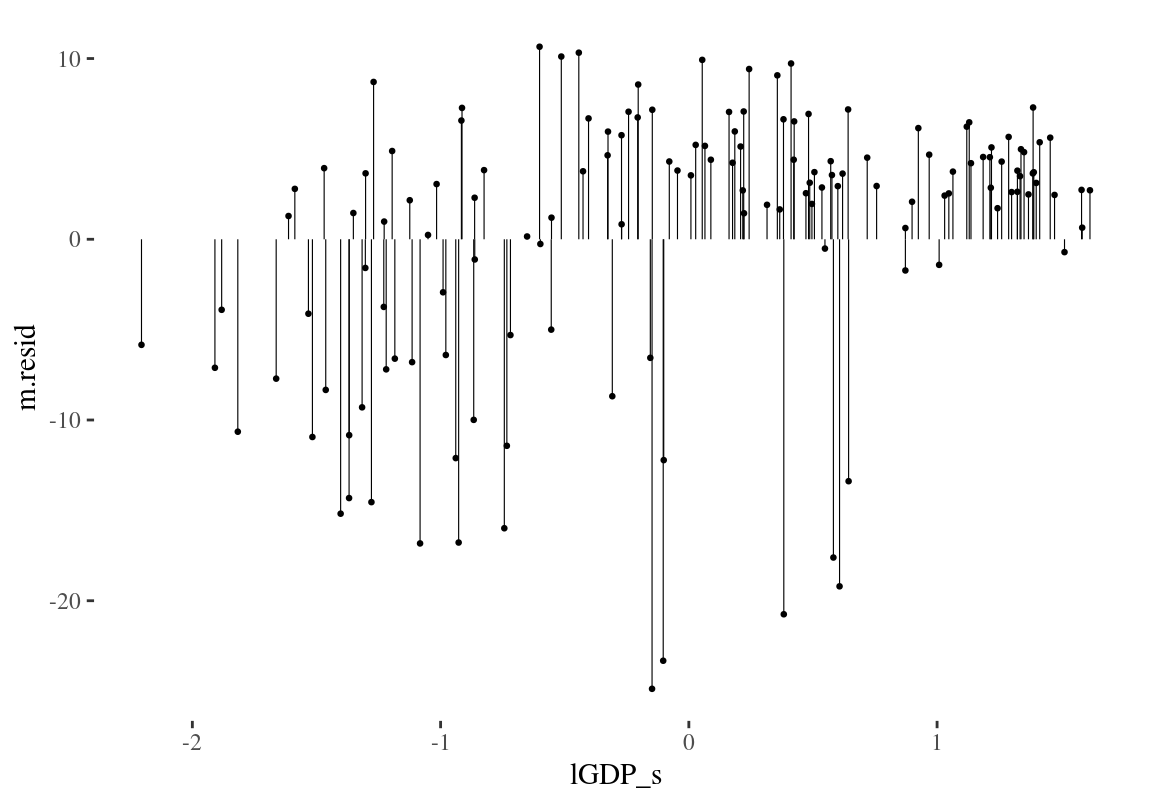
\includegraphics[width=0.7\linewidth]{04_lineaarsed_mudelid_files/figure-latex/unnamed-chunk-7-1} 

}

\caption{Lineaarne mudel, mille lõikepunkt = 0 ja tõus = 3. Katkendjoon, tõus = 1. Pidevjoon, tõus = 3.}\label{fig:unnamed-chunk-7}
\end{figure}

Nüüd muutub sirge tõusunurk, ehk kui palju me ootame \emph{y}-t
muutumas, kui \emph{x} muutub näiteks ühe ühiku võrra. Kui b = 3, siis
\emph{x}-i tõustes ühe ühiku võrra suureneb \emph{y} kolme ühiku võrra.
Proovi järgi, mis juhtub, kui b = -3.

Selleks, et sirget kahes dimensioonis vabalt liigutada, piisab kui me
kombineerime eelnevad näited ühte:

\[y = a + b \times x\]

Selleks lisame mudelisse kaks parameetrit, lõikepunkt (a) ja tõus (b).
Kui \(a = 0\) ja \(b = 1\), saame me eelpool kirjeldatud mudeli
\(y = x\). Kui \(a = 102\), siis sirge lõikab y-telge väärtusel 102. Kui
\(b = 0.8\), siis x-i tõustes 1 ühiku võrra tõuseb y-i väärtus 0.8 ühiku
võrra. Kui \(a = 100\) ja \(b = 0\), siis saame sirge, mis on paraleelne
x-teljega ja lõikab y-telge väärtusel 100. Seega, teades a ja b väärtusi
ning omistades x-le suvalise meid huvitava väärtuse, saab ennustada y-i
keskmist väärtust sellel x-i väärtusel. Näiteks, olgu andmete vastu
fititud mudel pikkus(cm) = 102 + 0.8 * kaal(kg) ehk

\[y = 102 + 0.8 \times x\]

Omistades nüüd kaalule väärtuse 80 kg, tuleb mudeli poolt ennustatud
keskmine pikkus 102 + 0.8 * 80 = 166 cm. Iga kg lisakaalu ennustab
mudeli kohaselt 0.8 cm võrra suuremat pikkust.

\begin{Shaded}
\begin{Highlighting}[]
\NormalTok{a <-}\StringTok{ }\DecValTok{102}
\NormalTok{b <-}\StringTok{ }\FloatTok{0.8}
\NormalTok{x <-}\StringTok{  }\DecValTok{0}\OperatorTok{:}\DecValTok{100} 
\NormalTok{y <-}\StringTok{  }\NormalTok{a }\OperatorTok{+}\StringTok{ }\NormalTok{b }\OperatorTok{*}\StringTok{ }\NormalTok{x}
\end{Highlighting}
\end{Shaded}

\begin{Shaded}
\begin{Highlighting}[]
\KeywordTok{plot}\NormalTok{(y }\OperatorTok{~}\StringTok{ }\NormalTok{x, }\DataTypeTok{xlab =} \StringTok{"Weight in kg"}\NormalTok{, }\DataTypeTok{ylab =} \StringTok{"Heigth in cm"}\NormalTok{, }\DataTypeTok{ylim =} \KeywordTok{c}\NormalTok{(}\DecValTok{50}\NormalTok{, }\DecValTok{200}\NormalTok{), }\DataTypeTok{type =} \StringTok{"l"}\NormalTok{, }\DataTypeTok{main =} \KeywordTok{bquote}\NormalTok{(y }\OperatorTok{==}\StringTok{ }\DecValTok{102} \OperatorTok{+}\StringTok{ }\FloatTok{0.8} \OperatorTok\StringTok{ }\NormalTok{x))}
\end{Highlighting}
\end{Shaded}

\begin{figure}

{\centering 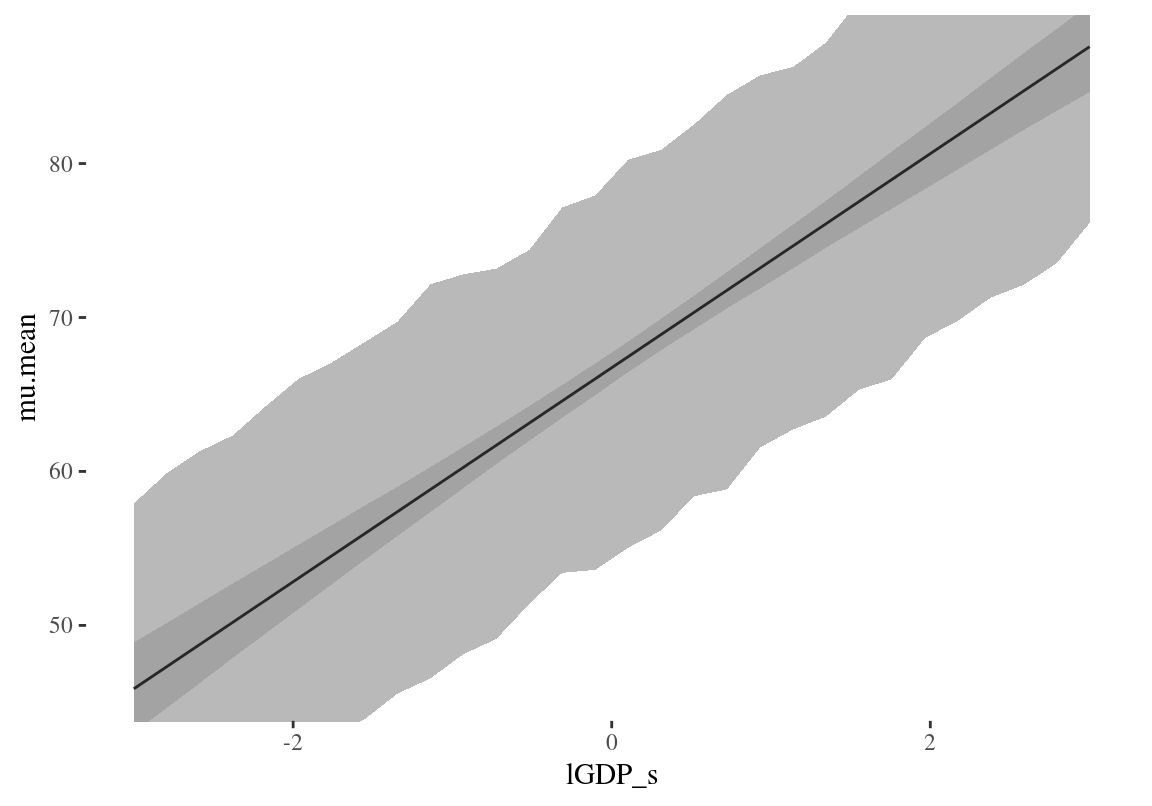
\includegraphics[width=0.7\linewidth]{04_lineaarsed_mudelid_files/figure-latex/unnamed-chunk-9-1} 

}

\caption{Lineaarne mudel, millel on tuunitud nii lõikepunkt kui tõus.}\label{fig:unnamed-chunk-9}
\end{figure}

See mudel ennustab, et 0 kaalu juures on pikku 102 cm, mis on rumal, aga
mudelite puhul tavaline olukord. Sellel olukorral on mitmeid põhjusi:

\begin{itemize}
\item
  Me tuunime mudelit andmete peal, mis ei sisalda 0-kaalu.
\item
  Meie valimiandmed ei peegelda täpselt inimpopulatsiooni.
\item
  Sirge mudel ei peegelda täpselt pikkuse-kaalu suhteid vahemikus, kus
  meil on reaalseid kaaluandmeid; ja ta teeb seda veelgi vähem seal, kus
  meil mõõdetud kaalusid ei ole.
\end{itemize}

Seega pole mõtet imestada, miks mudeli intercept meie üle irvitab.

Kahe parameetriga sirge mudel ongi see, mida me fitime
kahedimensiooniliste andmetega.

Näiteks nii, kasutame R-i ``iris'' andmesetti:

\begin{Shaded}
\begin{Highlighting}[]
\CommentTok{# Fit a linear model and name the model object as m}
\NormalTok{m <-}\StringTok{ }\KeywordTok{lm}\NormalTok{(Sepal.Length }\OperatorTok{~}\StringTok{ }\NormalTok{Petal.Length, }\DataTypeTok{data =}\NormalTok{ iris)}
\end{Highlighting}
\end{Shaded}

\begin{Shaded}
\begin{Highlighting}[]
\CommentTok{# Make a scatter plot, colored by the var called "Species"}
\CommentTok{# Draw the fitted regression line from m}
\KeywordTok{augment}\NormalTok{(m, iris) }\OperatorTok\StringTok{ }
\StringTok{  }\KeywordTok{ggplot}\NormalTok{(}\KeywordTok{aes}\NormalTok{(Petal.Length, Sepal.Length, }\DataTypeTok{color =}\NormalTok{ Species)) }\OperatorTok{+}
\StringTok{  }\KeywordTok{geom_point}\NormalTok{() }\OperatorTok{+}
\StringTok{  }\KeywordTok{geom_line}\NormalTok{(}\KeywordTok{aes}\NormalTok{(}\DataTypeTok{y =}\NormalTok{ .fitted), }\DataTypeTok{color =} \DecValTok{1}\NormalTok{) }\OperatorTok{+}
\StringTok{  }\KeywordTok{labs}\NormalTok{(}\DataTypeTok{title =} \StringTok{"Sepal.Length ~ Petal.Length"}\NormalTok{) }\OperatorTok{+}
\StringTok{  }\KeywordTok{scale_color_viridis}\NormalTok{(}\DataTypeTok{discrete =} \OtherTok{TRUE}\NormalTok{)}
\end{Highlighting}
\end{Shaded}

\begin{figure}

{\centering 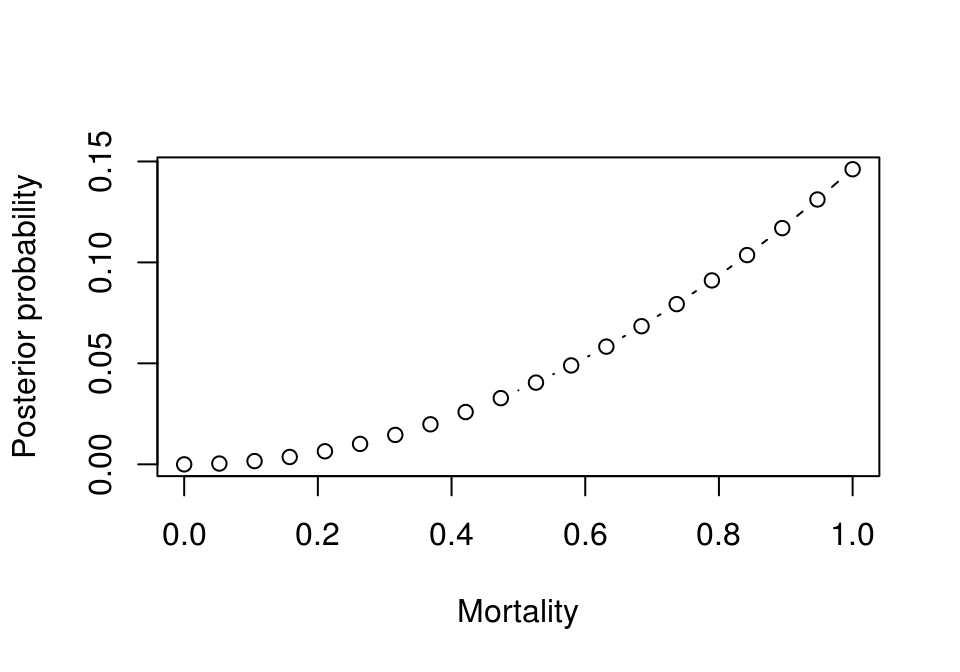
\includegraphics[width=0.7\linewidth]{04_lineaarsed_mudelid_files/figure-latex/unnamed-chunk-11-1} 

}

\caption{Fititud mudel, kus muutuja Petal.Length järgi ennustatakse muutuja Sepal.Length väärtusi.}\label{fig:unnamed-chunk-11}
\end{figure}

Mudeli fittimine tähendab siin lihtsalt, et sirge on 2D ruumi asetatud
nii, et see oleks võimalikult lähedal kõikidele punktidele.

\begin{quote}
Oletame, et meil on n andmepunkti ja et me fitime neile sirge. Nüüd
plotime fititud sirge koos punktidega ja tõmbame igast punktist
mudelsirgeni joone, mis on paraleelne y-teljega. Seejärel mõõdame nende
n joone pikkused. Olgu need pikkused a, b, \ldots{} i. \texttt{lm()}
funktsioon fitib sirge niimoodi, et summa \(a^2 + b^2 + ... + i^2\)
oleks minimaalne. Seda kutsutakse vähimruutude meetodiks.
\end{quote}

Mudeli koefitsientide väärtused saame kasutades funktsiooni
\texttt{coef()}:

\begin{Shaded}
\begin{Highlighting}[]
\KeywordTok{coef}\NormalTok{(m)}
\CommentTok{#>  (Intercept) Petal.Length }
\CommentTok{#>        4.307        0.409}
\end{Highlighting}
\end{Shaded}

Siin a = (Intercept) ja b = Petal.Length ehk 0.41.

\section{Ennustus lineaarsest
mudelist}\label{ennustus-lineaarsest-mudelist}

Anname x-le rea väärtusi, et ennustada y keskmisi väärtusi nendel x-i
väärtustel. Siin me ennustame y (Sepal\_length) keskväärtusi erinevatel
x-i (Petal\_length) väärtustel, mitte individuaalseid Sepal\_length
väärtusi. Me kasutame selleks deterministlikku mudelit kujul
Sepal\_length = a + b*Petal\_length. Hiljem õpime ka bayesiaanlike
meetoditega individuaalseid Sepal\_length-e ennustama.

Järgnev kood on sisuliselt sama, millega me üle-eelmisel plotil
joonistasime mudeli y = a + bx. Me fikseerime mudeli koefitsiendid
fititud irise mudeli omadega ja anname Petal\_length muutujale 10
erinevat väärtust originaalse muutuja mõõtmisvahemikus. Aga sama hästi
võiksime ekstrapoleerida ja küsida, mis on oodatav Sepal\_length, kui
Petal\_length on 100 cm? Sellele küsimusele on ebareaalne vastus, aga
mudel ei tea seda. Proovi, mis vastus tuleb.

\begin{Shaded}
\begin{Highlighting}[]
\NormalTok{## Genereerime uued andmed Petal.Length vahemikus}
\NormalTok{Petal_length <-}\StringTok{ }\KeywordTok{seq}\NormalTok{(}\KeywordTok{min}\NormalTok{(iris}\OperatorTok{$}\NormalTok{Petal.Length), }
                    \KeywordTok{max}\NormalTok{(iris}\OperatorTok{$}\NormalTok{Petal.Length), }
                    \DataTypeTok{length.out =} \DecValTok{10}\NormalTok{)}
\NormalTok{## Võtame mudeli koefitsendid}
\NormalTok{a <-}\StringTok{ }\KeywordTok{coef}\NormalTok{(m)[}\DecValTok{1}\NormalTok{]}
\NormalTok{b <-}\StringTok{ }\KeywordTok{coef}\NormalTok{(m)[}\DecValTok{2}\NormalTok{]}
\NormalTok{## Kasutades mudeli koefitsente genereerime Sepal_length väärtused}
\NormalTok{Sepal_length <-}\StringTok{  }\NormalTok{a }\OperatorTok{+}\StringTok{ }\NormalTok{b }\OperatorTok{*}\StringTok{ }\NormalTok{Petal_length}
\end{Highlighting}
\end{Shaded}

\begin{Shaded}
\begin{Highlighting}[]
\KeywordTok{plot}\NormalTok{(Sepal_length }\OperatorTok{~}\StringTok{ }\NormalTok{Petal_length, }\DataTypeTok{type =} \StringTok{"b"}\NormalTok{)}
\end{Highlighting}
\end{Shaded}

\begin{figure}

{\centering 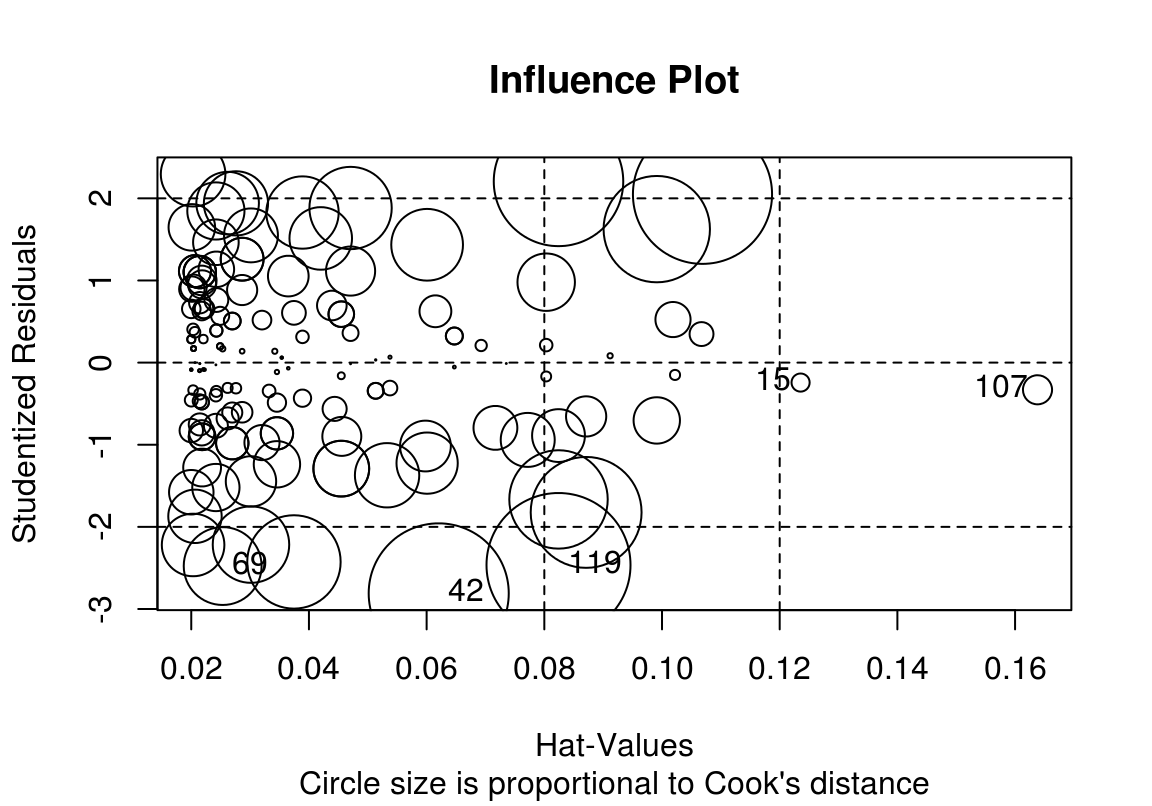
\includegraphics[width=0.7\linewidth]{04_lineaarsed_mudelid_files/figure-latex/unnamed-chunk-14-1} 

}

\caption{Siin ennustasime kümme y väärtust x väärtuste põhjal..}\label{fig:unnamed-chunk-14}
\end{figure}

\begin{quote}
Mudelist saab kahte tüüpi ennustusi: interpolatsioone (ennustus on samas
skaalas, mis andmed, mille peal mudel fititi) ja ekstrapoleerimine
(ennustus jääb väljaspoole andmeid). Sõltuvalt erialast me kas vaatame
ekstrapoleerimisele viltu või leiame, et selline tegevus on otsesõnu
keelatud.
\end{quote}

\begin{quote}
Mudelist saab kahte tüüpi ennustusi: (1) saame ennustada Y keskmist
väärtust X-i konkreetsel väärtusel ja (2) saame ennustada
individuaalseid Y väärtusi X-i konkreetsel väärtusel. Viimase kohta vt
ptk\ldots{}
\end{quote}

\section{Neli mõistet}\label{neli-moistet}

Mudelis \(y = a + bx\) on \(x\) ja \(y\) muutujad, ning \(a\) ja \(b\)
on parameetrid. Muutujate väärtused fikseeritakse andmetega, parameetrid
fititakse andmete põhjal. Fititud mudel valib kõikide võimalike seda
tüüpi mudelite hulgast välja täpselt ühe unikaalse mudeli ja ennustab
igale \(x\)-i väärtusele vastava kõige tõenäolisema \(y\) väärtuse
(\(y\) keskväärtuse sellel \(x\)-i väärtusel).

\begin{itemize}
\item
  Y --- mida me ennustame (\emph{dependent variable, predicted
  variable}).
\item
  X --- mille põhjal me ennustame (\emph{independent variable,
  predictor}).
\item
  Muutuja (variable) --- iga asi, mida me valimis mõõdame (X ja Y on
  kaks muutujat). Muutujal on sama palju fikseeritud väärtusi kui meil
  on selle muutuja kohta mõõtmisandmeid.
\item
  Parameeter (parameter) --- mudeli koefitsient, millele võib omistada
  suvalisi väärtusi. Parameetreid tuunides fitime mudeli võimalikult
  hästi sobituma andmetega.
\end{itemize}

Mudel on matemaatilise formalism, mis püüab kirjeldada füüsikalist
protsessi. Statistilise mudeli struktuuris on komponent, mis kirjeldab
ideaalseid ennustusi (nn protsessi mudel) ja eraldi veakomponent (ehk
veamudel), mis kirjeldab looduse varieeruvust nende ideaalsete
ennustuste ümber. Mudeli koostisosad on (i) muutuja, mille väärtusi
ennustatakse, (ii), muutuja(d), mille väärtuste põhjal ennustatakse,
(iii) parameetrid, mille väärtused fititakse ii põhjal ja (iv)
konstandid.

\section{Mudeli fittimine}\label{mudeli-fittimine}

Mudelid sisaldavad nii (1) matemaatilisi struktuure, mis määravad mudeli
tüübi, kui (2) parameetreid, mida saab andmete põhjal tuunida, niiviisi
täpsustades mudeli kuju ehk paiknemist matemaatlises ruumis. Näiteks
võrrand \(y = a + bx\) määrab mudeli, kus \(y = x\) on see struktuur,
mis tagab, et mudeli tüüp on sirge, ning \(a\) ja \(b\) on parameetrid,
mis määravad sirge asendi. Seevastu struktuur \(y = x + x^2\) tagab, et
mudeli \(y = a + b_1x + b_2x^2\) tüüp on parabool, ning parameetrite
\(a\), \(b_1\) ja \(b_2\) väärtused määravad selle parabooli täpse kuju.
Ja nii edasi.

Mudeli parameetrite tuunimist nimetatakse mudeli fittimiseks. Mudelit
fittides on eesmärk saavutada antud tüüpi mudeli maksimaalne sobivus
andmetega (kus ``andmed'' hõlmavad nii valimiandmeid kui
taustateadmisi). Sellele tegevusele annab mõtte meie lootus, et mudeli
tüüp kajastab mingit looduses toimuvat protsessi, mis meile teaduslikku
huvi pakub. Ning, kuigi mudeli fit maksimeeritakse mudeli tüübi kohta,
püüab see andmete vaatenurgast vaadatuna olla optimaalne, mitte
maksimaalne (vt järgmine peatükk mudeli üle- ja alafittimisest). Kahjuks
ei ole selline optimaalsus kuigi hästi matemaatilisse vormi valatav, ega
ka mingi (pool)automaatse meetodiga empiiriliselt kontrollitav. Siin on
tegu pigem teadlase sooviga, mille filosoofiline eeldus on, et meie
andmetes on peidus nii andmeid genereeriva loodusliku protsessi üldine
olemus (essents), kui juhuslik müra ehk valimiviga, ning et mudeli
üldine kuju (sirge, parabool, jms) on juhtumisi sobiv just selleks, et
neid kahte omavahel lahku ajada.

\begin{quote}
Lineraarse mudeli parima sobivuse andmetega saab tagada kahel erineval
viisil: (i) vähimruutude meetod (Legendre, 1805; Gauss, 1809) mõõdab y
telje suunaliselt iga andmepunkti kauguse mudeli ennustusest, võtab
selle kauguse ruutu, summeerib kauguste ruudud ning leiab sirge asendi,
mille korral see summa on minimaalne; (ii) Bayesi teoreem (Laplace,
1774) annab väheinformatiivse priori korral praktiliselt sama fiti.
Olulise erinevusena võtab vähimruutude meetod arvesse ainult
valimiandmed, samas kui Bayesi teoreemi kasutades fitime mudeli
koefitsiente nii valimiandmete kui taustateadmiste peal (vt 8. ptk).
\end{quote}

Hea mudel on

\begin{enumerate}
\def\labelenumi{\arabic{enumi}.}
\item
  Võimalikult lihtsa struktuuriga, mille põhjal on veel võimalik teha
  järeldusi protsessi kohta, mis genereeris mudeli fittimiseks kasutatud
  andmeid;
\item
  Sobitub piisavalt hästi andmetega (eriti uute andmetega, mida ei
  kasutatud selle mudeli fittimiseks), et olla relevantne andmeid
  genereeriva protsessi kirjeldus;
\item
  Genereerib usutavaid simuleeritud andmeid.
\end{enumerate}

Sageli fititkse samade andmetega mitu erinevat tüüpi mudelit ja püütakse
otsustada, milline neist vastab kõige paremini eeltoodud tingimustele.
Näiteks, kui sirge suudab kaalu järgi pikkust ennustada paremini kui
parabool, siis on sirge mudel paremas kooskõlas teadusliku hüpoteesiga,
mis annaks mehhanismi protsessile, mille käigus kilode lisandumine viiks
laias kaaluvahemikus inimeste pikkuse kasvule ilma, et pikkuse kasvu
tempo kaalu tõustes langeks. Samas, see et me oleme oma andmeid fittinud
n mudeliga ja otsustanud, et mõned neist on paremad kui teised, ei
tähenda, et mõni meie mudelitest oleks hea ka võrdluses tegeliku
looduses valitseva olukorraga. Mudelid on pelgalt matemmatilised
formalismid, mis võivad, aga kindlasti ei pea, kajastama füüsikalist
maailma, ja meie mudelitevalik sõltub meile jõukohasest matemaatikast.
Siinkohal ei tasu unustada, et matemaatika kirjeldab eelkõige
abstraktseid mustreid, mitte otse füüsikalist maailma.

See, et teie andmed sobivad hästi mingi mudeliga, ei tähenda
automaatselt, et see fakt oleks teaduslikult huvitav. Mudeli parameetrid
on mõtekad mudeli matemaatilise kirjelduse kontekstis, aga mitte
tingimata suure maailma põhjusliku seletamise kontekstis. Siiski, kui
mudeli matemaatiline struktuur loodi andmeid genreeeriva loodusliku
protsessi olemust silmas pidades, võib mudeli koefitsientide uurimisest
selguda olulisi tõsiasju suure maailma kohta.

\begin{quote}
Mudeli fittimine: X ja Y saavad oma väärtused otse andmetest;
parameetrid võivad omandada ükskõik millise väärtuse.
\end{quote}

\begin{quote}
Fititud mudelist ennustamine: X-le saab omistada ükskõik millise
väärtuse; parameetrite väärtused on fikseeritud; Y väärtus arvutatakse
mudelist.
\end{quote}

\subsection{Üle- ja alafittimine}\label{ule--ja-alafittimine}

Osad mudelite tüübid on vähem paindlikud kui teised (parameetreid
tuunides on neil vähem liikumisruumi). Kuigi sellised mudelid sobituvad
halvemini andmetega, võivad need ikkagi paremini kui mõni paindlikum
mudel välja tuua andmete peidetud olemuse. Statistiline mudeldamine
eeldab, et me usume, et meie andmetes leidub nii müra (mida mudel võiks
ignoreerida), kui signaal (mida mudel püüab tabada). Ilma signaalita
süsteemi poleks arusaadavatel põhjustel mõtekas mudeldada ja ilma mürata
süsteemi mudel tuleks ilma varieeruvuse (vea) komponendita, ehk
deterministlik. Kuna mudeli jaoks näeb müra samamoodi välja kui signaal,
on iga mudel kompromiss üle- ja alafittimise vahel. Me lihtsalt loodame,
et meie mudel on piisavalt jäik, et mitte liiga palju müra modelleerida
ja samas piisavalt paindlik, et piisaval määral signaali tabada.

Üks kõige jäigemaid mudeleid on sirge, mis tähendab, et sirge mudel on
suure tõenäosusega alafittitud. Keera sirget kuipalju tahad, ikka ei
sobitu ta enamiku andmekogudega. Ja need vähesed andmekogud, mis sirge
mudeliga sobivad, on genereeritud teatud tüüpi lineaarsete protsesside
poolt. Sirge on seega üks kõige paremini tõlgendatavaid mudeleid. Teises
äärmuses on polünoomsed mudelid, mis on väga paindlikud, mida on väga
raske tõlgendada ja mille puhul esineb suur mudeli ülefittimise oht.
Ülefititud mudel järgib nii täpselt valimiandmeid, et sobitub hästi
valimis leiduva juhusliku müraga ning seetõttu sobitub halvasti järgmise
valimiga samast populatsioonist (igal valimil on oma juhuslik müra).
Üldiselt, mida rohkem on mudelis tuunitavaid parameetreid, seda
paindlikum on mudel, seda kergem on seda valimiandmetega sobitada ja
seda raskem on seda tõlgendada. Veelgi enam, alati on võimalik
konstrueerida mudel, mis sobitub täiuslikult kõikide andmepunktidega
(selle mudeli parameetrite arv = N). Selline mudel on täpselt sama
informatiivne kui andmed, mille põhjal see fititi --- ja täiesti kasutu.

\begin{verbatim}
#> Warning: `cols` is now required.
#> Please use `cols = c(preds)`
\end{verbatim}

\begin{figure}

{\centering 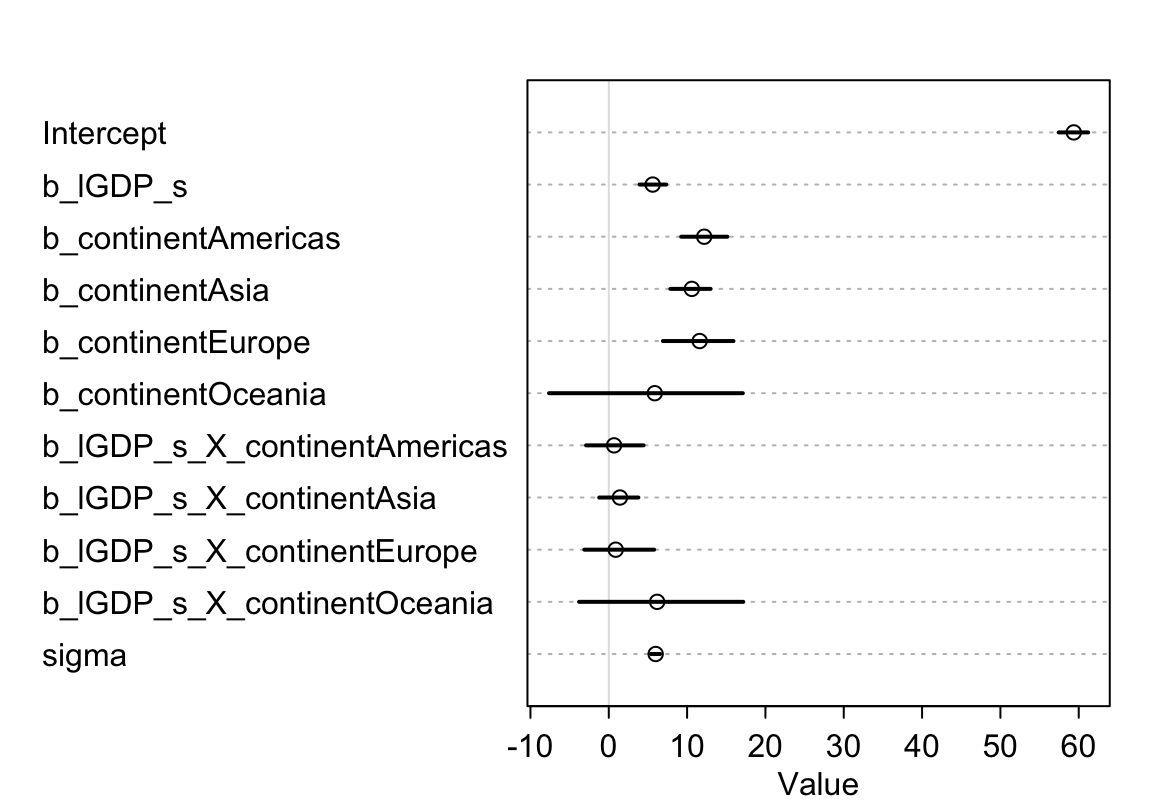
\includegraphics[width=0.7\linewidth]{04_lineaarsed_mudelid_files/figure-latex/unnamed-chunk-16-1} 

}

\caption{Kasvava paindlikusega polünoomsed mudelid.}\label{fig:unnamed-chunk-16}
\end{figure}

Vähimruutude meetodil fititud mudeleid saame võrrelda AIC-i näitaja
järgi. AIC - Akaike Informatsiooni Kriteerium - vaatab mudeli sobivust
andmetega ja mudeli parameetrite arvu. Väikseim AIC tähitab parimat
fitti väikseima parameetrite arvu juures (kompromissi) ja väikseima
AIC-ga mudel on eelistatuim mudel. Aga seda ainult võrreldud mudelite
hulgas. AIC-i absoluutväärtus ei loe - see on suhteline näitaja.

\begin{tabular}{lr}
\toprule
model\_formula & aic\\
\midrule
y \textasciitilde{} x & 35.0\\
y \textasciitilde{} poly(x, 2) & 37.0\\
y \textasciitilde{} poly(x, 3) & 36.1\\
y \textasciitilde{} poly(x, 4) & 32.5\\
y \textasciitilde{} poly(x, 5) & -Inf\\
\bottomrule
\end{tabular}

AIC näitab, et parim mudel on mod\_e4. Aga kas see on ka kõige kasulikum
mudel? Mis siis, kui 3-s andmepunkt on andmesisestaja näpuviga?

\begin{quote}
Ülefittimise vältimiseks kasutavad Bayesi mudelid informatiivseid
prioreid, mis välistavad ekstreemsed parameetriväärtused. Vt
\url{http://elevanth.org/blog/2017/08/22/there-is-always-prior-information/}
\end{quote}

\section{Lineaarse regressiooni
eeldused}\label{lineaarse-regressiooni-eeldused}

\subsection*{Matemaatilised eeldused:}\label{matemaatilised-eeldused}
\addcontentsline{toc}{subsection}{Matemaatilised eeldused:}

\begin{enumerate}
\def\labelenumi{\arabic{enumi}.}
\item
  Lineaarsus: ennustus Y-muutujale on lineaarne funktsioon
  prediktoritest \(Y = \beta_1X_1 + \beta_2X_2 +···\beta_nX_n\), ehk
  ekvivalentselt: kõikidel X-i väärtustel keksmine residuaal = 0.
\item
  homoskedastilisus ehk konstantne Y-muutuja suunaline varieeruvus
  kõigil X-i väärtustel. See tähendab ühtlasi residuaalide konstantset
  varieeruvust.
\item
  Normaalsus - residuaalid on normaaljaotusega, ehk Y-muutuja on
  normaaljaotusega kõigil X-i väärtustel.
\item
  Sõltumatus - residuaalide väärtused ei ole omavahel korreleeritud.
\item
  X-muutuja suunal puudub mõõtmisviga ja ebakindlus, mis tähendab, et
  x-i väärtused on täpselt teada (me ei ennusta neid). See eeldus on
  tähtis siis, kui püüame anda regresioonimudelile põhjusliku
  tõlgenduse. Mudelis \(Y = \alpha + \beta_1X_1 + \beta_2X_2\) viib
  mõõtmisviga \(X_2\)-s \(\beta_2\) koefitsiendi nulli suunas ja ühtlasi
  vähendab \(\beta_2X_2\) liikme mõju \(\beta_1\) fittimisel.
\item
  X-muutuja ei ole konstant vaid sisaldab erinevaid väärtusi.
\item
  Mitme prediktoriga lineaarse regressiooni puhul tuleb sisse veel
  kollineaarsuse eeldus: me eeldame, et ükski prediktorite paar pole
  täiuslikult lineaarselt korreleeritud (pole lineaarne funktsioon
  üksteisest).
\end{enumerate}

\subsection*{Eeldused praktilise tähtsuse
järjekorras:}\label{eeldused-praktilise-tahtsuse-jarjekorras}
\addcontentsline{toc}{subsection}{Eeldused praktilise tähtsuse
järjekorras:}

\begin{enumerate}
\def\labelenumi{\arabic{enumi}.}
\item
  Valiidsus -- sa mõõdad asju, mis on relevantsed teadusliku küsimuse
  seisukohast. Näiteks, kui soovite mõõta kolesterooli alandava ravimi
  mõju, on mõistlik mõõta suremust, mitte pelgalt kolesterooli taset
  veres.
\item
  Esinduslikkus -- andmed peaksid olema esinduslikud laiema
  populatsiooni suhtes. Väikesed ja kallutatud valimid ei ole sageli
  esinduslikud.
\item
  Lineaarsus ja sellest tulenev mudeli additiivsus. Väga tähtis on, et
  lineaarse regressiooniga mõõdetavad seosed oleks ka tõesti lineaarsed.
  Kui lineaarsusega on probleeme, võib aidata prediktorite
  transformeerimine (log(x) või 1/x) või uute prediktorite mudelisse
  lisamine. Samuti on võimalik prediktoritena samasse mudelisse panna
  nii \(x\) kui \(x^2\). Näiteks kui me paneme mudelisse nii muutuja
  \(vanus\) kui ka \(vanus^2\), saame modelleerida seost, kus y vanuse
  kasvades alguses kasvab ja siis kahaneb (aga ka U kujulist seost
  vanusega). Sellisel juhul võib olla ka mõistlik rekodeerida vanus
  kategooriliseks muutujaks (näit 4 vanuseklassi), mille tasemeid saab
  siis ükshaaval vaadata.
\item
  Sõltumatus. Selle eelduse rikkumine viib liiga kitsastele
  usalduspiiridele.
\item
  Vigade võrdne varieeruvus (homoskedastilisus) ja vigade normaalsus on
  vähemtähtsad. Log-normaalsete vigadega võiks lineaarsel regresioonil
  mudeldada log(Y) skaalas (vähimruutude meetodil) või Bayesi
  regressioonil mittelineaarset lognormaalset tõepäramudelit kasutades
  (vt. ptk 13).
\item
  Kollineaarsus. Täieliku kolineaarsuse korral mudel ei lahendu, aga
  sellisel juhul on põhjuseks enamasti viga mudeli spetsifitseerimisel.
  Osaline, aga ikkagi väga kõrge, kollineaarsus, mis õnneks on praktikas
  pigem haruldane, viib koefitsientide laiadele veapiiridele. Kui
  veapiirid pole laiad, siis pole ka kollineaarsust.
\end{enumerate}

\subsection*{Regressioon kui kirjeldus ja kui põhjuslik
hüpotees}\label{regressioon-kui-kirjeldus-ja-kui-pohjuslik-hupotees}
\addcontentsline{toc}{subsection}{Regressioon kui kirjeldus ja kui
põhjuslik hüpotees}

Regressioonanalüüsi võib vaadelda 1) empiirilise kirjeldusena y ja x-i
koos-varieerumisest või 2) muutujate vaheliste põhjuslike suhete
analüüsina. Esimesel juhul ei tõlgenda me x ja y suhet x-i mõjuna y-le.
Seega, senikaua kui mudeli fit väljaspool andmeid, mida kasutati selle
mudeli fittimiseks, on piisavalt hea, ei ole võimalik, et me fitime vale
struktuuriga mudeli. Kui me fitime 2 mudelit (i)
\(Y = \alpha + \beta_1X_1\) ja (ii)
\(Y = \alpha + \beta_1X_1 + \beta_2X_2\), siis eeldame, et kahe mudeli
\(\beta_1\) koefitsiendid tulevad erinevad. Aga sellest pole midagi,
sest need kirjeldavad mõlemal juhul vaid empiirilisi seoseid.

Teisel, põhjuslikul juhul on kõik teisiti. Eeldades et \(X_2\) on üks
Y-i põhjustest, on nüüd esimese mudeli veakomponendis peidus ka
\(\beta_2X_2\). Kui \(X_1\) ja \(X_2\) on omavahel korreleeritud, siis
tekib meil seetõttu ka korrelatsioon \(X_1\) ja veakomponendi vahel --
ja see rikub mudeli eeldusi, kallutades mudeli fittimisel meie hinnangut
\(\beta_1\)-le, misläbi osa \(X_2\) mõjust Y-le omistatakse ekslikult
\(X_1\)-le. See kõik juhtub siis, kui teise mudeli \(\beta_2\) ei ole
null ja esineb \(X_1\) ja \(X_2\) vaheline korrelatsioon.

Selle kallutatuse tõlgendamine sõltub omakorda \(X_1\) ja \(X_2\)
vahelise põhjusliku seose struktuurist. Oluline on mõista, et mudeli
enda struktuuris pole vähimatki põhjuslikku infot - mudel ei tea isegi
sellise asja nagu põhjuslikkus olemasolust. Seega on meil lisaks
regressioonimudelile vaja sellest iseseisvat põhjuslikku mudelit, mille
formuleerime puhtalt teaduslikest asjaoludest lähtuvalt.

Kõige lihtsam selline mudel vastab randomiseeritud ja kontrollitud
eksperimendile, kus me võrdleme katse ja kontrolltingimusi. Siin me
usume, et kui katsetingimuse rakendamine (näiteks ravimi manustamine)
mõjutab mingis kindlas suunas katse väljundit (näiteks suremust), ja
seda võrreldes kontrolltingimusega (näiteks platseeboga), siis me oleme
näidanud, et vastav ravim vähendab suremust. Seega on meie põhjuslik
skeem ravim --\textgreater{} suremus ja regressioonimudel
suremus\textasciitilde{}ravim, mis sisuliselt taandub kahe grupi
keskmiste suremuste võrdlusele.

Kuidas on aga asjalood siis, kui meil ei lubata katset teha? Näiteks,
kuidas määrata suitsetamise mõju kopsuvähile? Siin ei ole meil tegemist
randomiseeritud katsega (me ei tohi jagada populatsiooni juhuslikult
kahte gruppi ja sundida neist ühte suitsetama). Seega peame kasutama
statistilisi meetodeid, et kontrollida oma tulemust nn confounderite
vastu. Siin on lihtsaim võimalus regressioonimudel vähk
\textasciitilde{} suitsetamine + muutuja\_1 + \ldots{}

Aga muutujaid on maailmas palju ja meil peab olema mingi reegel, mille
järgi otsustada, millised muutujad additiivsesse mudelisse sisse panna
ja millised välja jätta. Mudeli ennustusjõu maksimeerimine siin ei aita.
Selle asemel peame mõistma võimalike põhjuslike skeemide suhet mitmese
regressioonimudelitega. Põhjuslikud skeemid on nagu legod, mis koosnevad
järgmistest põhiosistest e ehitusplokkidest.

\begin{enumerate}
\def\labelenumi{\arabic{enumi}.}
\item
  toru: x --\textgreater{} z --\textgreater{} y
\item
  kahvel: x \textless{}-- z --\textgreater{} y
\item
  laupkokkupõrge: x --\textgreater{} z \textless{}-- y
\item
  järglane: see on toru, kus z-i juurest hargneb veel üks nool A-le.
  Siin saame me mudelisse A lisades ligikaudu sama tulemuse, mis z-i
  lisades. Seega, kui z-i väärtused pole meile teada, võime hädaga ka
  A-d kasutada.
\end{enumerate}

Kui me tahame teada, kas x mõjutab y-t, siis toru puhul mudel
\(y ~ x + z\) vähendab x-i mõju (sest see mõju käib läbi z-i). Samas,
mudel \(y ~ x\) näitab x-i mõju. Seega, kumba mudelit kasutada sõltub
sellest, kas me tahame näidata x-i otsest või kaudset mõju y-ile.

Kahvli puhul regressioonimudel \(y ~ x\) näitab x-i mõju y-le (ehkki
meie põhjuslikkuse mudelis puudub x ja y vaheline põhjuslik seos), aga
mudel \(y ~ x + z\) välistab selle mõju. Seega peaksime sellise
põhjusliku hüpoteesi korral mudelisse z-i sisse panema, sest see aitab
kontrollida z konfounding mõju vastu.

Laupkokkupõrke korral on olukord eelnevaga vastupidine. Nüüd avab mudel
\(y ~ x + z\) tagaukse ja laseb z-i segava mõju mudelisse sisse, mis
tekitab meile võlts-põhjusliku suhte x ja y vahel.

Näiteks võib meil tekkid olukord, kus testime suitsetamise mõju vähile,
aga me usume, et inimeste vanus mõjutab iseseisvalt nii vähki kui
suitsetamist (vanemad inimesed surevad rohkem, aga nad ka suitsetavad
rohkem). Selles põhjuslikus skeemis töötab vanus kahvlina, millega
arvestamiseks tuleb see regressioonimudelisse muutujana sisse panna:
vähk \textasciitilde{} suitsetamine + vanus.

\chapter{Kaks lineaarse mudeli
laiendust}\label{kaks-lineaarse-mudeli-laiendust}

\begin{Shaded}
\begin{Highlighting}[]
\KeywordTok{library}\NormalTok{(tidyverse)}
\KeywordTok{library}\NormalTok{(scatterplot3d)}
\KeywordTok{library}\NormalTok{(viridis)}
\KeywordTok{library}\NormalTok{(ggeffects)}
\KeywordTok{library}\NormalTok{(broom)}
\KeywordTok{library}\NormalTok{(car)}
\end{Highlighting}
\end{Shaded}

\section{Mitme sõltumatu prediktoriga
mudel}\label{mitme-soltumatu-prediktoriga-mudel}

Esiteks vaatame mudelit, kus on mitu prediktorit \(x_1\), \(x_2\),
\ldots{} \(x_n\), mis on aditiivse mõjuga. See tähendab, et me liidame
nende mõjud, mis omakorda tähendab, et me usume, et \(x_1\) \ldots{}
\(x_n\) mõjud y-i väärtusele on üksteisest sõltumatud. Mudel on siis
kujul

\[y = a + b_1x_1~ + b_2x_2~ +~ ... +~ b_nx_n\]

\begin{quote}
Mitme prediktoriga mudeli iga prediktori tõus (beta koefitsient) ütleb,
mitme ühiku võrra ennustab mudel y muutumist juhul kui see prediktor
muutub ühe ühiku võrra ja kõik teised prediktorid ei muutu üldse (Yule,
1899).
\end{quote}

Milliseid muutujaid (regressoreid) peaks üks hea lineaarne mudel
sisaldama, milliseid peaks me mudelist välja viskama ja milliseid igal
juhul sisse panema? Matemaatiliselt põhjustab regressorite eemaldamine
ülejäänud regressorite koefitsientide ebakonsistentsust, välja arvatud
siis, kui (i) välja visatud regressorid ei ole korreleeritud sisse
jäetud regressoritega või (ii) välja vistatud regressorite koefitsiendid
võrduvad nulliga, mis muudab nad ebarelevantseteks. Kuidas sa tead, et
kõik vajalikud regressorid on sul üldse olemas (olematuid andmeid ei saa
ka mudelisse lisada)? Loomulikult ei teagi, mis tähendab lihtsalt, et
mudeldamine on keeruline protsess, nagu teaduski. Pane ka tähele, et
koefitsiendi ``mitte-oluline'' p väärtus ei tähenda iseenesest, et
koefitsient tõenäoliselt võrdub nulliga või on nulli lähedal, vaid seda,
et meil pole piisavalt andmeid, et vastupidist kinnitada. Koefitsiendi
hinnangu usalduspiirid on selles osas palju parem töövahend.

Kui meie andmed on kolmedimensionaalsed (me mõõdame igal mõõteobjektil
kolme muutujat) ja me tahame ennnustada ühe muutuja väärtust kahe teise
muutuja väärtuste põhjal (meil on kaks prediktorit), siis tuleb meie
kolme parameetriga lineaarne regressioonimudel tasapinna kujul. Kui meil
on kolme prediktoriga mudel, siis me liigume juba neljamõõtmelisse
ruumi.





\begin{figure}
\centering
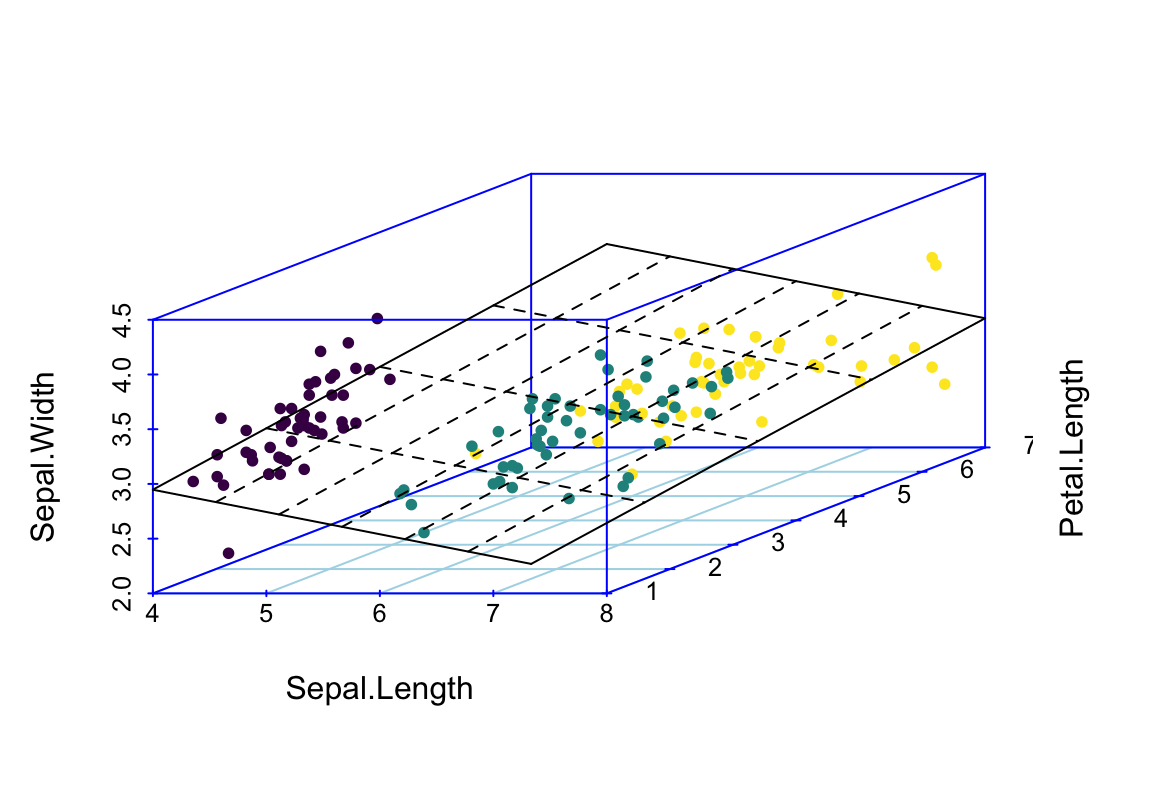
\includegraphics{05_lin_mudeli_laiendused_files/figure-latex/regressioonitasand-1.pdf}
\caption{\label{fig:regressioonitasand}Regressioonitasand 3D andmetele. Kahe
prediktoriga mudel, kus Sepal.Length ja Petal.Length on prediktorid ja
Sepal.Width ennustatav muutuja.}
\end{figure}

Seda mudelit saab kaeda 2D ruumis, kui kollapseerida kolmas mõõde
konstandile.






\begin{Shaded}
\begin{Highlighting}[]
\NormalTok{p <-}\StringTok{ }\KeywordTok{ggplot}\NormalTok{(iris, }\KeywordTok{aes}\NormalTok{(Sepal.Length, Sepal.Width, }\DataTypeTok{color =}\NormalTok{ Species)) }\OperatorTok{+}
\StringTok{  }\KeywordTok{geom_point}\NormalTok{() }\OperatorTok{+}
\StringTok{  }\KeywordTok{xlim}\NormalTok{(}\DecValTok{4}\NormalTok{, }\DecValTok{8}\NormalTok{) }\OperatorTok{+}
\StringTok{  }\KeywordTok{scale_color_viridis}\NormalTok{(}\DataTypeTok{discrete =} \OtherTok{TRUE}\NormalTok{) }\OperatorTok{+}
\StringTok{  }\KeywordTok{theme}\NormalTok{(}\DataTypeTok{title =} \KeywordTok{element_text}\NormalTok{(}\DataTypeTok{size =} \DecValTok{8}\NormalTok{))}
\NormalTok{p1 <-}\StringTok{ }\NormalTok{p }\OperatorTok{+}\StringTok{ }\KeywordTok{geom_abline}\NormalTok{(}\DataTypeTok{intercept =} \KeywordTok{coef}\NormalTok{(m2)[}\DecValTok{1}\NormalTok{], }\DataTypeTok{slope =} \KeywordTok{coef}\NormalTok{(m2)[}\DecValTok{2}\NormalTok{]) }\OperatorTok{+}
\StringTok{  }\KeywordTok{labs}\NormalTok{(}\DataTypeTok{title =} \KeywordTok{deparse}\NormalTok{(}\KeywordTok{formula}\NormalTok{(m2)))}
\NormalTok{m1 <-}\StringTok{ }\KeywordTok{lm}\NormalTok{(Sepal.Width }\OperatorTok{~}\StringTok{ }\NormalTok{Sepal.Length, }\DataTypeTok{data =}\NormalTok{ iris)}
\NormalTok{p2 <-}\StringTok{ }\NormalTok{p }\OperatorTok{+}\StringTok{ }\KeywordTok{geom_abline}\NormalTok{(}\DataTypeTok{intercept =} \KeywordTok{coef}\NormalTok{(m1)[}\DecValTok{1}\NormalTok{], }\DataTypeTok{slope =} \KeywordTok{coef}\NormalTok{(m1)[}\DecValTok{2}\NormalTok{]) }\OperatorTok{+}
\StringTok{  }\KeywordTok{labs}\NormalTok{(}\DataTypeTok{title =} \KeywordTok{deparse}\NormalTok{(}\KeywordTok{formula}\NormalTok{(m1)))}
\NormalTok{devtools}\OperatorTok{::}\KeywordTok{source_gist}\NormalTok{(}\StringTok{"8b4d6ab6a333ef1cd14e8067c3badbae"}\NormalTok{, }\DataTypeTok{filename =} \StringTok{"grid_arrange_shared_legend.R"}\NormalTok{)}
\KeywordTok{grid_arrange_shared_legend}\NormalTok{(p1, p2)}
\end{Highlighting}
\end{Shaded}

\begin{figure}
\centering
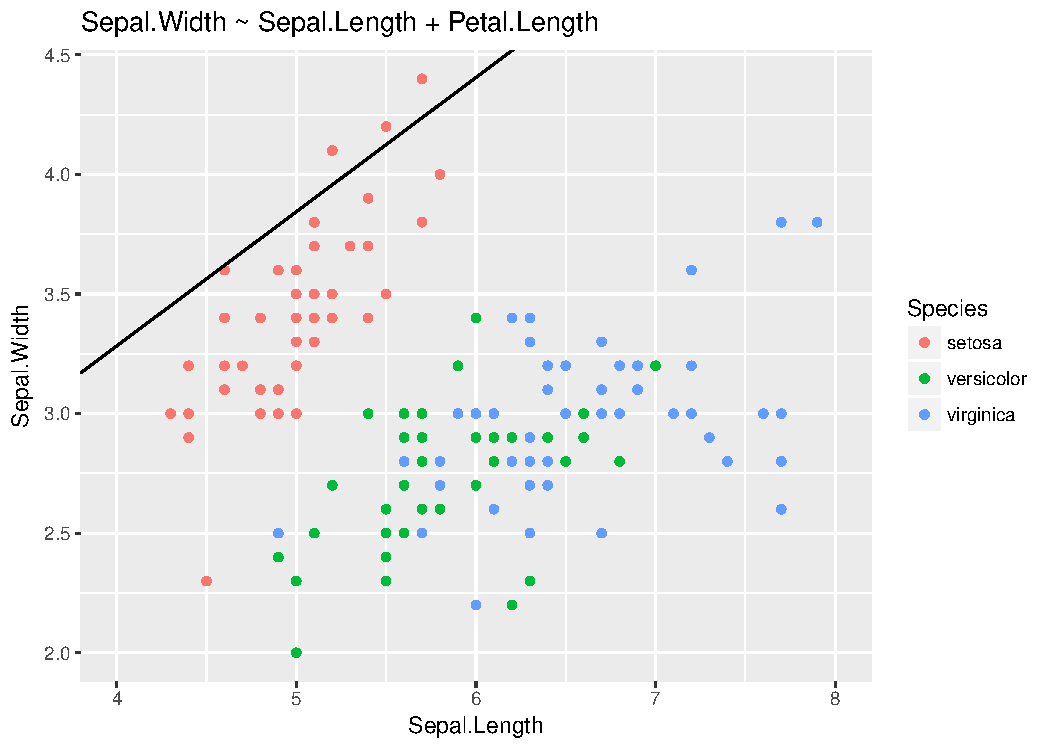
\includegraphics{05_lin_mudeli_laiendused_files/figure-latex/lin2d-1.pdf}
\caption{\label{fig:lin2d}2D-le kollapseeritud graafiline kujutus 3D andmete põhjal
fititud mudelist. Vasemal, muutuja Petal.Length on kollapseeritud
konstandile. Siin on regressioonijoon hoopis teises kohas, kui lihtsas
ühe prediktoriga mudelis (paremal).}
\end{figure}

Võrreldes mudelite m1 (üks prediktor) ja m2 (kaks prediktorit)
Sepal.Length (\(b_1\)) koefitsienti on näha, et need erinevad oluliselt.

\begin{Shaded}
\begin{Highlighting}[]
\KeywordTok{coef}\NormalTok{(m1)}
\CommentTok{#>  (Intercept) Sepal.Length }
\CommentTok{#>       3.4189      -0.0619}
\KeywordTok{coef}\NormalTok{(m2)}
\CommentTok{#>  (Intercept) Sepal.Length Petal.Length }
\CommentTok{#>        1.038        0.561       -0.335}
\end{Highlighting}
\end{Shaded}

Kumb mudel on siis parem? AIC-i järgi on m2 kõvasti parem kui m1,
lisakoefitsendi (Petal.Length) kaasamisel mudelisse paranes oluliselt
selle ennustusvõime.

\begin{Shaded}
\begin{Highlighting}[]
\KeywordTok{AIC}\NormalTok{(m1, m2)}
\CommentTok{#>    df   AIC}
\CommentTok{#> m1  3 179.5}
\CommentTok{#> m2  4  92.1}
\end{Highlighting}
\end{Shaded}

\subsection*{Ennustused sõltumatute prediktoritega
mudelist}\label{ennustused-soltumatute-prediktoritega-mudelist}
\addcontentsline{toc}{subsection}{Ennustused sõltumatute prediktoritega
mudelist}

Siin on idee kasutada fititud mudeli struktuuri ennustamaks y keskmisi
väärtusi erinevatel \(x_1\) ja \(x_2\) väärtustel. Kuna mudel on
fititud, on parameetrite väärtused fikseeritud.

\begin{Shaded}
\begin{Highlighting}[]
\NormalTok{## New sepal length values}
\NormalTok{Sepal_length <-}\StringTok{ }\KeywordTok{seq}\NormalTok{(}\KeywordTok{min}\NormalTok{(iris}\OperatorTok{$}\NormalTok{Sepal.Length), }\KeywordTok{max}\NormalTok{(iris}\OperatorTok{$}\NormalTok{Sepal.Length), }\DataTypeTok{length.out =} \DecValTok{10}\NormalTok{)}
\NormalTok{## Keep new petal length constant}
\NormalTok{Petal_length <-}\StringTok{ }\KeywordTok{mean}\NormalTok{(iris}\OperatorTok{$}\NormalTok{Petal.Length)}
\NormalTok{## Extract model coeficents}
\NormalTok{a <-}\StringTok{ }\KeywordTok{coef}\NormalTok{(m2)[}\StringTok{"(Intercept)"}\NormalTok{]}
\NormalTok{b1 <-}\StringTok{ }\KeywordTok{coef}\NormalTok{(m2)[}\StringTok{"Sepal.Length"}\NormalTok{]}
\NormalTok{b2 <-}\StringTok{ }\KeywordTok{coef}\NormalTok{(m2)[}\StringTok{"Petal.Length"}\NormalTok{]}
\NormalTok{## Predict new sepal width values}
\NormalTok{Sepal_width_predicted <-}\StringTok{ }\NormalTok{a }\OperatorTok{+}\StringTok{ }\NormalTok{b1 }\OperatorTok{*}\StringTok{ }\NormalTok{Sepal_length }\OperatorTok{+}\StringTok{ }\NormalTok{b2 }\OperatorTok{*}\StringTok{ }\NormalTok{Petal_length}
\end{Highlighting}
\end{Shaded}





\begin{Shaded}
\begin{Highlighting}[]
\KeywordTok{plot}\NormalTok{(Sepal_width_predicted }\OperatorTok{~}\StringTok{ }\NormalTok{Sepal_length, }\DataTypeTok{type =} \StringTok{"b"}\NormalTok{, }\DataTypeTok{ylim =} \KeywordTok{c}\NormalTok{(}\DecValTok{0}\NormalTok{, }\DecValTok{5}\NormalTok{), }\DataTypeTok{col =} \StringTok{"red"}\NormalTok{)}
\CommentTok{# Prediction from the single predictor model}
\KeywordTok{abline}\NormalTok{(m1, }\DataTypeTok{lty =} \StringTok{"dashed"}\NormalTok{)}
\end{Highlighting}
\end{Shaded}

\begin{figure}
\centering
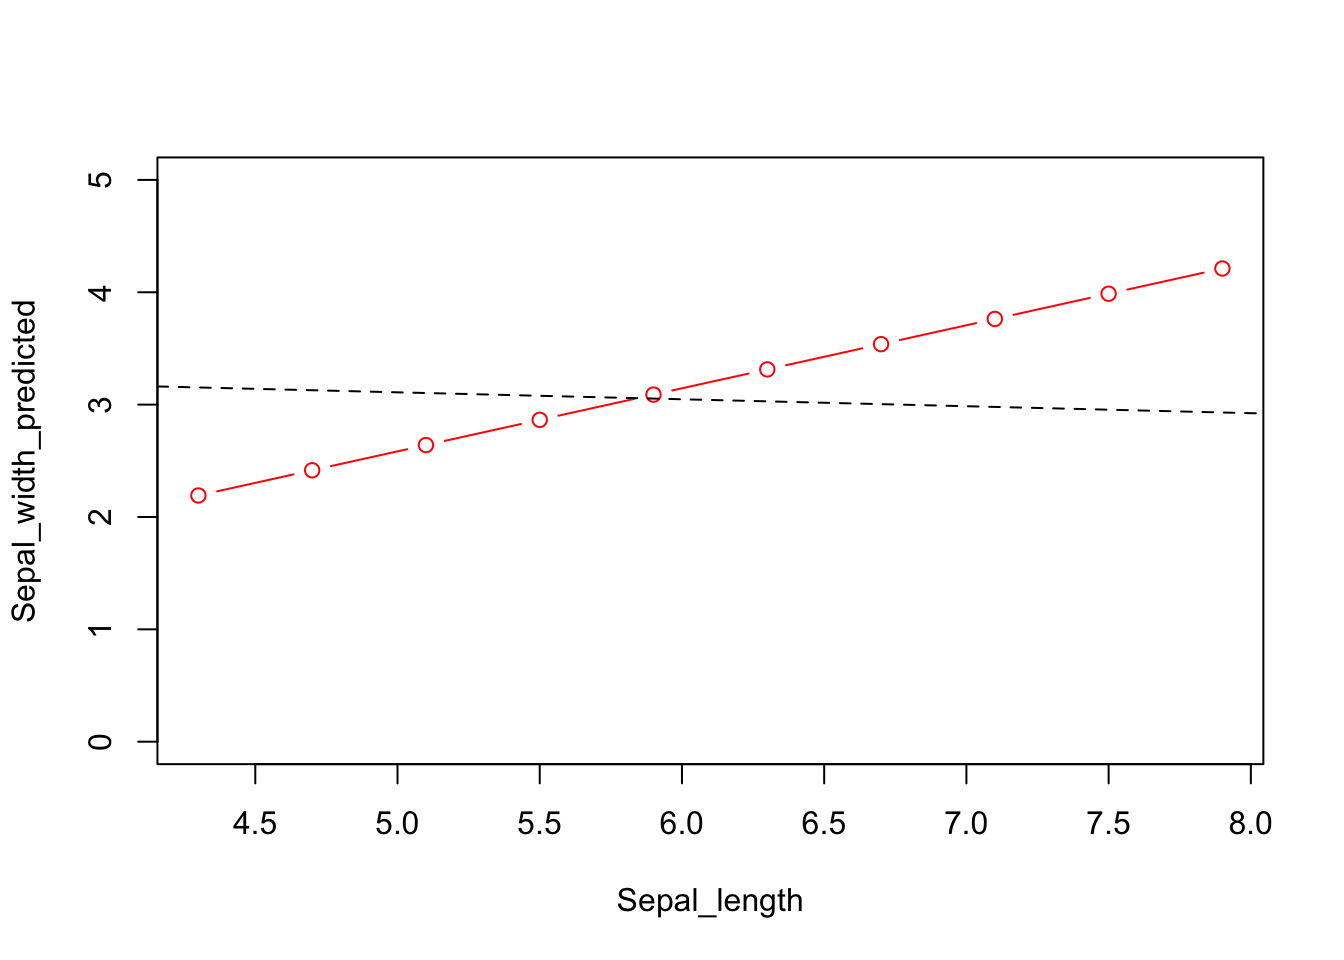
\includegraphics{05_lin_mudeli_laiendused_files/figure-latex/yksversuskaks-1.pdf}
\caption{\label{fig:yksversuskaks}Ennustatud y väärtused erinevatel \(x_1\) väärtustel
kui \(x_2\) on konstantne, punane joon. Katkendjoon, ühe prediktoriga
mudeli ennustus.}
\end{figure}

Nüüd joonistame 3D pildi olukorrast, kus nii x\textsubscript{1} kui
x\textsubscript{2} omandavad rea väärtusi. Mudeli ennustus on ikkagi
sirge kujul -- mis sest, et 3D ruumis.



\begin{verbatim}
#> Warning: `data_frame()` is deprecated, use `tibble()`.
#> This warning is displayed once per session.
\end{verbatim}

\begin{figure}
\centering
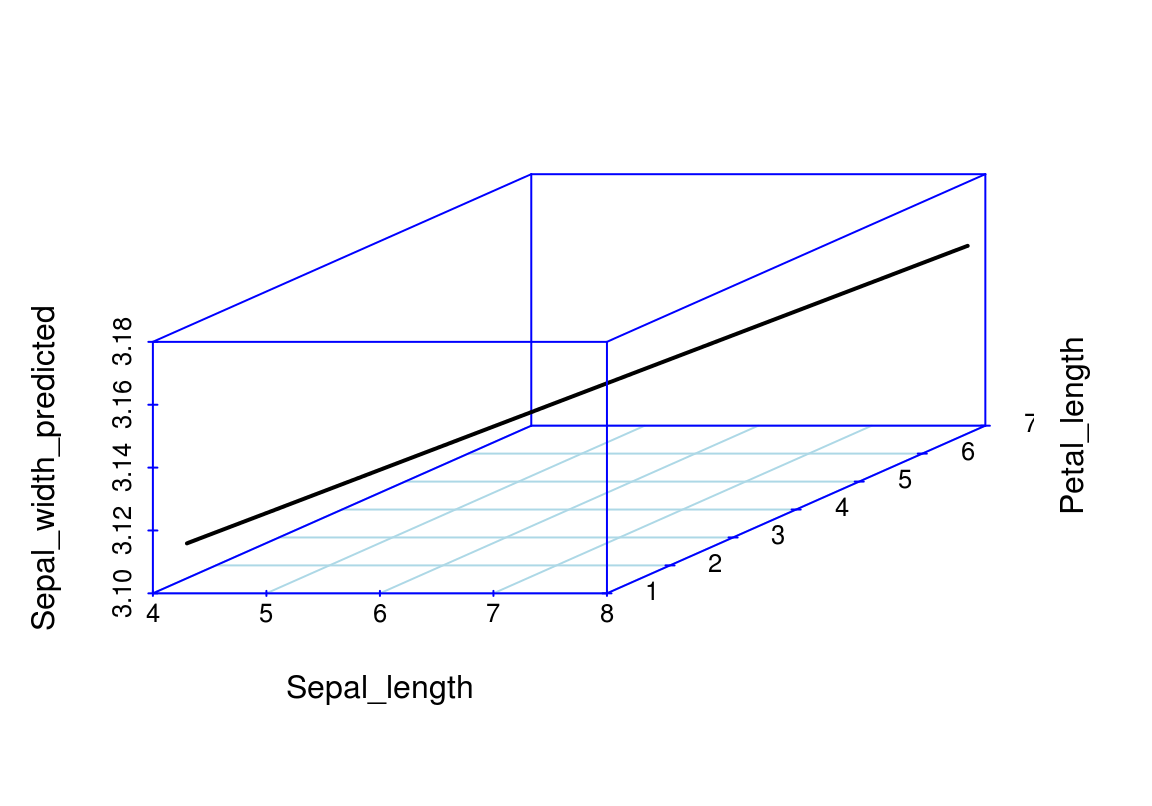
\includegraphics{05_lin_mudeli_laiendused_files/figure-latex/kaksprediktorit-1.pdf}
\caption{\label{fig:kaksprediktorit}Kahe prediktoriga mudeli ennustus 3D ruumis.}
\end{figure}

\section{Interaktsioonimudel}\label{interaktsioonimudel}

Interaktsioonimudelis sõltub ühe prediktori mõju teise prediktori
väärtusest:

\[y = a + b_1x_1 + b_2x_2 + b_3x_1x_2\]

Ekvivalntne viis interaktsiooni spetsifitseerida on läbi
võrrandisüsteemi: \[y = a + \gamma x_1 + b_2x_2\]
\[\gamma = b_1 + b_3x_2\] Siit on hästi näha, et me teeme kaks
lineaarset regressiooni, millest teine modelleerib \(x_1\) muutuja
koefitsiendi sõltuvust \(x_2\) muutuja väärtusest.

Samamoodi kehtib ka ümberkirjutus \[y = a + \gamma x_2 + b_1x_1\]
\[\gamma = b_2 + b_3x_1\]

mis tähendab, et ühtlasi modelleerime me ka \(x_2\) koefitsiendi
sõltuvust \(x_1\)-st. Mudeli koefitsientide tõlgendamise teeb
keeruliseks, et gamma tõlgendamisel tuleb arvesse võtta kolm asja --
b\textsubscript{2}, b\textsubscript{3} ja x\textsubscript{1}.

Kaks muutujat võivad inteakteeruda sõltumata sellest, kas nad on
korreleeritud või mitte -- interaktsioon ei impitseeri korrelatsiooni,
ega vastupidi.

Sageli on nii, et prediktoreid, mille mõju y-le on suur, tasub mudeldada
ka interaktsioonimudelis (näiteks suitsetamise mõju vähimudelites kipub
olema interaktsiooniga). Interaktsioonimudelis on b\textsubscript{1}
koefitsient otse tõlgendatav ainult siis, kui x\textsubscript{2} = 0 (ja
b\textsubscript{2} ainult siis, kui x\textsubscript{1} = 0).

Kui interaktsioonimudel fititakse tsentreeritud x-muutujate peal, mille
keskväärtus = 0 (või standardiseeritud muutujatel), siis muutub
koefitsientide tõlgendamine lihtsamaks:

\begin{itemize}
\item
  b\textsubscript{1} annab y tõusu, kui x\textsubscript{1} tõuseb 1
  ühiku võrra ja x\textsubscript{2} on fikseeritud oma keskväärtusel
\item
  b\textsubscript{2} annab y tõusu, kui x\textsubscript{2} tõuseb 1
  ühiku võrra ja x\textsubscript{1} on fikseeritud oma keskväärtusel).
\item
  b\textsubscript{3} ütleb, kui palju muutub x\textsubscript{1} mõju
  y-le, kui x\textsubscript{2} muutub ühe ühiku võrra. Samamoodi,
  b\textsubscript{3} ütleb, kui palju muutub x\textsubscript{2} mõju
  y-le, kui x\textsubscript{1} muutub ühe ühiku võrra.
\end{itemize}

NB! Ärge standardiseerige faktormuutujaid ehk \emph{dummy}-regressoreid
kujul 1, 0 -- neid on lihtsam tõlgendada algsel kujul 0/1 skaalas.

Edaspidi õpime selliseid mudeleid graafiliselt tõlgendama, kuna
koefitsientide otse tõlgendamine ei ole siin sageli perspektiivikas.

\begin{quote}
Interaktsioonimudelis sõltub x\textsubscript{1} mõju tugevus y-le
x\textsubscript{2} väärtusest. Selle sõltuvuse määra kirjeldab
b\textsubscript{3} (x\textsubscript{1} ja x\textsubscript{2}
interaktsiooni tugevus). Samamoodi ja sümmeetriliselt erineb ka
x\textsubscript{2} mõju erinevatel x\textsubscript{1} väärtustel. Ainult
siis, kui x\textsubscript{2} = 0, ennustab x\textsubscript{1} tõus 1
ühiku võrra y muutust b\textsubscript{1} ühiku võrra.
\end{quote}

Kui meil on mudelis interaktsiooniliige \(x_1x_2\), siis on enamasti
mõistlik ka lisada eraldi liikmetena ka \(x_1\) ja \(x_2\).

Näiteks mudel, milles on pidev y-muutuja, pidev prediktor ``education''
ja binaarne prediktor ``sex\_male'' (1 ja 0):

\[score = a + b_1 * education + b_2 * sex_{male} + b_3 * education * sex_{male}\]

Variandis

\[score = a + b_1 * education + b_3 * education * sex_{male}\]

surume meeste ja naiste intercepti pidevale muutujale ``education'' ühte
punkti, aga samas modelleerime sellele erinevad tõusud meeste ja naiste
lõikes.

Samamoodi, variandis

\[score = a +  b_2 * sex_{male} + b_3 * education * sex_{male}\]

on naiste tõus surutud nulli, aga interceptid võivad erineda, mis on
kokkuvõttes üsna imelik, kuigi tehniliselt on mudel ok ja seda võib
edukalt fittida.

Ja variandis

\[score = 0 + b_3 * education * sex_{male}\]

On meil meeste ja naiste intercept surutud nulli, aga meeste ja naiste
tõusud võivad erineda.

Kui meil on kaks faktor-prediktorit, siis mudel kujul

\[y= 0 + b_3x_1x_2\]

Mudeldab eraldi nende faktorite tasemete kõikvõimalud kombinatsioonid.

\begin{quote}
Oletame, et meil on lisaks pidevale prediktorile x\textsubscript{1} ka
faktor-prediktor x\textsubscript{2}. Diskreetsed e faktor-prediktorid
rekodeeritakse automaatselt nn \emph{dummy}-muutujateks. Kahevalentse e
binaarse muutuja, näit sex = c(``male'', ``female''), korral läheb
regressioonivõrrandisse uus dummy-muutuja, sex\_female, kus kõik emased
on 1-d ja isased 0-d. Üldine intercept vastab siis isaste mõjule ja
sex\_female intercept annab emaste erinevuse isastest. Kui meil on
n-tasemega diskreetne muutuja, rekodeerime selle n-1
\emph{dummy}-muutujana, millest igaüks on 0/1 kodeeringus ja millest
igaühe interceptid annavad erinevuse null-taseme (selle taseme, mis ei
ole rekodeeritud \emph{dummy}-muutujana) interceptist. Mudeli
seisukohast pole oluline, millise faktortunnuse taseme me nulltasemeks
võtame. Terminoloogiliselt on meie n-tasemega faktortunnus \emph{seletav
muutuja} (\emph{explanatory variable}), millest tehakse n-1
\emph{regressorit}. Seega tehniliselt on mudeli liikmed regressorid,
mitte seletavad muutujad. Üks seletav muutuja võib anda välja mitu
regressorit (nagu eelmises näites) ja üks regressor võib põhineda mitmel
muutujal (näit x\textsubscript{1x}2 interaktsiooniterm).
\end{quote}

Interaktsioonimudeli 2D avaldus on kurvatuuriga tasapind, kusjuures
kurvatuuri määrab b\textsubscript{3}.

Interaktsiooniga mudel on AIC-i järgi pisut vähem eelistatud võrreldes
kahe prediktoriga mudeliga m2. Seega, eriti lihtsuse huvides, eelistame
m2-e.

\begin{Shaded}
\begin{Highlighting}[]
\NormalTok{m3 <-}\StringTok{ }\KeywordTok{lm}\NormalTok{(Sepal.Width }\OperatorTok{~}\StringTok{ }\NormalTok{Sepal.Length }\OperatorTok{+}\StringTok{ }\NormalTok{Petal.Length }\OperatorTok{+}\StringTok{ }\NormalTok{Sepal.Length }\OperatorTok{*}\StringTok{ }\NormalTok{Petal.Length, }\DataTypeTok{data =}\NormalTok{ iris)}
\KeywordTok{AIC}\NormalTok{(m1, m2, m3)}
\CommentTok{#>    df   AIC}
\CommentTok{#> m1  3 179.5}
\CommentTok{#> m2  4  92.1}
\CommentTok{#> m3  5  93.4}
\end{Highlighting}
\end{Shaded}

\subsection*{Ennustused
interaktsioonimudelist}\label{ennustused-interaktsioonimudelist}
\addcontentsline{toc}{subsection}{Ennustused interaktsioonimudelist}

Kõigepealt anname rea väärtusi x\textsubscript{1}-le ja hoiame
x\textsubscript{2} konstantsena.







\begin{Shaded}
\begin{Highlighting}[]
\NormalTok{Petal_length <-}\StringTok{  }\KeywordTok{mean}\NormalTok{(iris}\OperatorTok{$}\NormalTok{Petal.Length)}
\NormalTok{a <-}\StringTok{ }\KeywordTok{coef}\NormalTok{(m3)[}\StringTok{"(Intercept)"}\NormalTok{]}
\NormalTok{b1 <-}\StringTok{ }\KeywordTok{coef}\NormalTok{(m3)[}\StringTok{"Sepal.Length"}\NormalTok{]}
\NormalTok{b2 <-}\StringTok{ }\KeywordTok{coef}\NormalTok{(m3)[}\StringTok{"Petal.Length"}\NormalTok{]}
\NormalTok{b3 <-}\StringTok{ }\KeywordTok{coef}\NormalTok{(m3)[}\StringTok{"Sepal.Length:Petal.Length"}\NormalTok{]}
\NormalTok{Sepal_width_predicted <-}\StringTok{ }\NormalTok{a }\OperatorTok{+}\StringTok{ }\NormalTok{b1 }\OperatorTok{*}\StringTok{ }\NormalTok{Sepal_length }\OperatorTok{+}\StringTok{ }\NormalTok{b2 }\OperatorTok{*}\StringTok{ }\NormalTok{Petal_length }\OperatorTok{+}\StringTok{ }\NormalTok{b3 }\OperatorTok{*}\StringTok{ }\NormalTok{Sepal_length }\OperatorTok{*}\StringTok{ }\NormalTok{Petal_length}
\KeywordTok{plot}\NormalTok{(Sepal_width_predicted }\OperatorTok{~}\StringTok{ }\NormalTok{Sepal_length, }\DataTypeTok{type =} \StringTok{"l"}\NormalTok{, }\DataTypeTok{ylim =} \KeywordTok{c}\NormalTok{(}\DecValTok{2}\NormalTok{, }\DecValTok{6}\NormalTok{))}
\KeywordTok{abline}\NormalTok{(}\KeywordTok{coef}\NormalTok{(m2)[}\KeywordTok{c}\NormalTok{(}\StringTok{"(Intercept)"}\NormalTok{, }\StringTok{"Sepal.Length"}\NormalTok{)], }\DataTypeTok{lty =} \StringTok{"dashed"}\NormalTok{)}
\end{Highlighting}
\end{Shaded}

\begin{figure}
\centering
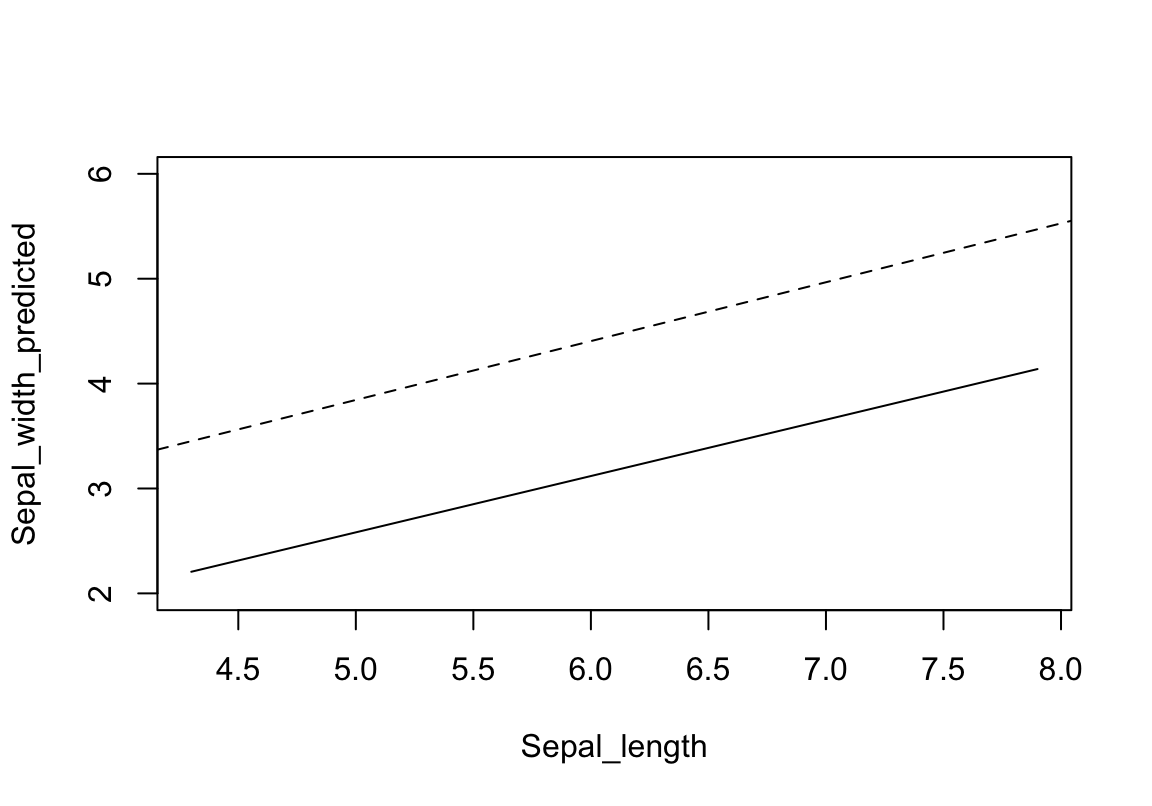
\includegraphics{05_lin_mudeli_laiendused_files/figure-latex/ennustus-interaktsioonimudelist-1.pdf}
\caption{\label{fig:ennustus-interaktsioonimudelist}Ennustus interaktsioonimudelist,
kus x\textsubscript{1} (Sepal\_Length) on antud rida väärtusi ja
x\textsubscript{2} (Petal\_length) hoitakse konstantsena (pidevjoon).
Interaktsioonimudeli regressioonijoon on paraleelne ilma
interaktsioonita mudeli ennustusele (katkendjoon).}
\end{figure}

Nagu näha viib korrutamistehe selleni, et interaktsioonimudeli tõus
erineb ilma interaktsioonita mudeli tõusust.

Kui aga interaktsioonimudel plottida välja 3D-s üle paljude
x\textsubscript{1} ja x\textsubscript{2} väärtuste, saame me
regressioonikurvi (mitte sirge), kus b\textsubscript{3} annab
kurvatuuri.





\begin{figure}
\centering
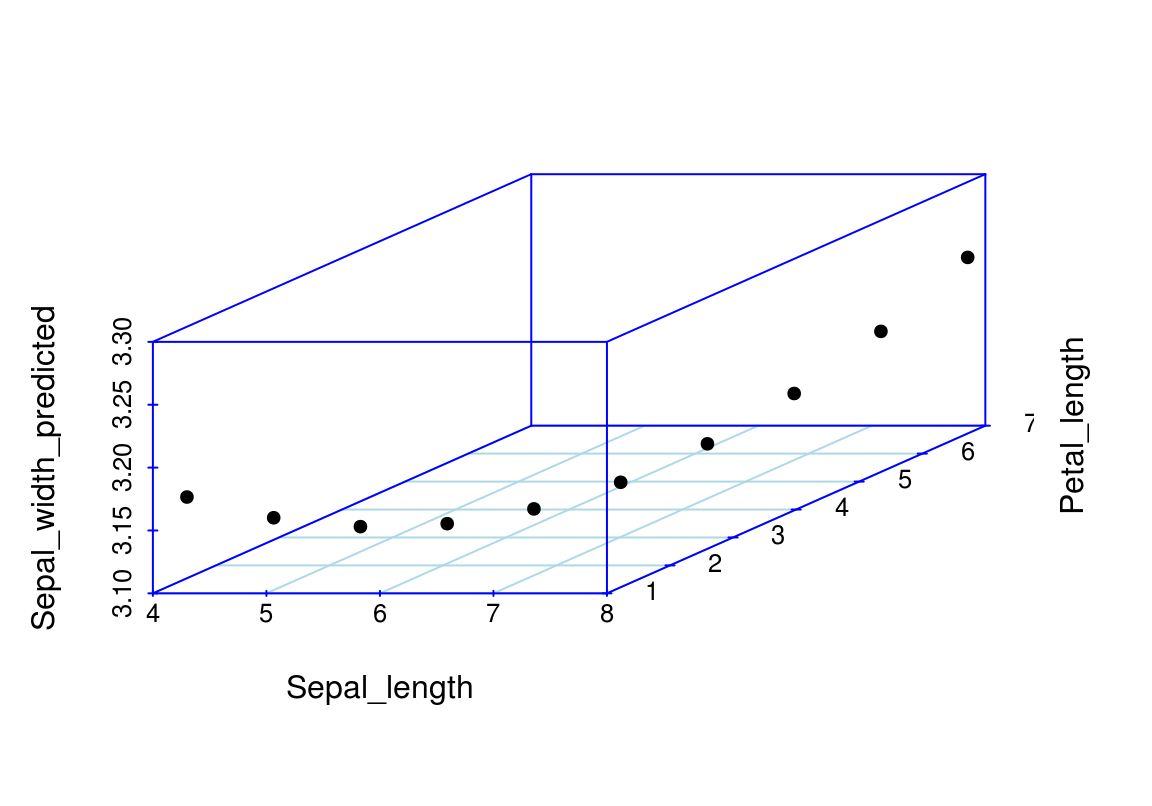
\includegraphics{05_lin_mudeli_laiendused_files/figure-latex/ennustused3d-interaktsioonimudelist-1.pdf}
\caption{\label{fig:ennustused3d-interaktsioonimudelist}Ennustused 3D
interaktsioonimudelist üle paljude x\textsubscript{1} (Sepal\_Length) ja
x\textsubscript{2} (Petal\_length) väärtuste.}
\end{figure}

Vau! See on alles ennustus!

\chapter{Vähimruutude meetodiga fititud mudelite töövoog --
lm()}\label{vahimruutude-meetodiga-fititud-mudelite-toovoog-lm}

Kuna lm() funktsiooniga ja bayesi meetodil fititud mudeliobjektidega
töötamine on mõnevõrra erinev, õpetame seda eraldi. Siinkohal anname
põhilise töövoo lm() mudelobjektide inspekteerimiseks.

Töötame m3 mudeliobjektiga, mis on interaktsioonimudel:

Sepal.Width \textasciitilde{} Sepal.Length * Species

ehk

\[Speal.Width = a + b_1*Sepal.Length + b_2*Species + b_3*Sepal.Length*Species\]

\begin{Shaded}
\begin{Highlighting}[]
\KeywordTok{library}\NormalTok{(ggeffects)}
\NormalTok{m3 <-}\StringTok{ }\KeywordTok{lm}\NormalTok{(Sepal.Width }\OperatorTok{~}\StringTok{ }\NormalTok{Sepal.Length }\OperatorTok{*}\StringTok{ }\NormalTok{Species, }\DataTypeTok{data =}\NormalTok{ iris)}
\end{Highlighting}
\end{Shaded}

\section*{1. vaatame mudeli
koefitsiente}\label{vaatame-mudeli-koefitsiente}
\addcontentsline{toc}{section}{1. vaatame mudeli koefitsiente}

\begin{Shaded}
\begin{Highlighting}[]
\KeywordTok{tidy}\NormalTok{(m3)}
\CommentTok{#> # A tibble: 6 x 5}
\CommentTok{#>   term                           estimate std.error statistic  p.value}
\CommentTok{#>   <chr>                             <dbl>     <dbl>     <dbl>    <dbl>}
\CommentTok{#> 1 (Intercept)                      -0.569     0.554     -1.03 3.06e- 1}
\CommentTok{#> 2 Sepal.Length                      0.799     0.110      7.23 2.55e-11}
\CommentTok{#> 3 Speciesversicolor                 1.44      0.713      2.02 4.51e- 2}
\CommentTok{#> 4 Speciesvirginica                  2.02      0.686      2.94 3.85e- 3}
\CommentTok{#> 5 Sepal.Length:Speciesversicolor   -0.479     0.134     -3.58 4.65e- 4}
\CommentTok{#> 6 Sepal.Length:Speciesvirginica    -0.567     0.126     -4.49 1.45e- 5}
\end{Highlighting}
\end{Shaded}

Interaktsioonimudeli koefitsientide jõllitamine on sageli tühi töö ja
vaimu närimine. Õnneks on meil muid meeotodeid, kuidas lm() mudelitega
töötada.

Võrdluseks - nii fitime eraldi mudeli igale irise liigile. Tulemus on
tegelikult identne interaktsioonimudeliga kategoorilisele muutujale
(Species), aga koefitsiendid on otse tõlgendatavad. Samas,
interaktsioonimudelit saab fittida ka pidevale muutujale!

\begin{Shaded}
\begin{Highlighting}[]
\NormalTok{iris }\OperatorTok\StringTok{ }\KeywordTok{split}\NormalTok{(.}\OperatorTok{$}\NormalTok{Species) }\OperatorTok\StringTok{ }
\StringTok{  }\KeywordTok{map}\NormalTok{(}\OperatorTok{~}\StringTok{ }\KeywordTok{lm}\NormalTok{(Sepal.Width }\OperatorTok{~}\StringTok{ }\NormalTok{Sepal.Length, }\DataTypeTok{data =}\NormalTok{ .)) }\OperatorTok\StringTok{ }
\StringTok{  }\KeywordTok{map}\NormalTok{(summary) }\OperatorTok\StringTok{ }
\StringTok{  }\KeywordTok{map_dfr}\NormalTok{(}\OperatorTok{~}\StringTok{ }\NormalTok{broom}\OperatorTok{::}\KeywordTok{tidy}\NormalTok{(.), }\DataTypeTok{.id =} \StringTok{"Species"}\NormalTok{)}
\CommentTok{#> # A tibble: 6 x 6}
\CommentTok{#>   Species    term         estimate std.error statistic  p.value}
\CommentTok{#>   <chr>      <chr>           <dbl>     <dbl>     <dbl>    <dbl>}
\CommentTok{#> 1 setosa     (Intercept)    -0.569    0.522      -1.09 2.81e- 1}
\CommentTok{#> 2 setosa     Sepal.Length    0.799    0.104       7.68 6.71e-10}
\CommentTok{#> 3 versicolor (Intercept)     0.872    0.445       1.96 5.56e- 2}
\CommentTok{#> 4 versicolor Sepal.Length    0.320    0.0746      4.28 8.77e- 5}
\CommentTok{#> 5 virginica  (Intercept)     1.45     0.431       3.36 1.55e- 3}
\CommentTok{#> 6 virginica  Sepal.Length    0.232    0.0651      3.56 8.43e- 4}
\end{Highlighting}
\end{Shaded}

Adjusteeritud r2 tasub eraldi üle vaadata.

\begin{Shaded}
\begin{Highlighting}[]
\KeywordTok{summary}\NormalTok{(m3)}\OperatorTok{$}\NormalTok{adj.r.squared}
\CommentTok{#> [1] 0.61}
\end{Highlighting}
\end{Shaded}

0.61 tähendab, et mudel suudab seletada mitte rohkem kui 61\% y-muutuja
(Sepal.Width) varieeruvusest.

\section*{2. Testime mudeli eeldusi}\label{testime-mudeli-eeldusi}
\addcontentsline{toc}{section}{2. Testime mudeli eeldusi}

Nii saab fititud väärtused (.fitted), residuaalid (.resid), fittitud
väätruste standardvead (.se.fit). Residuaal = y data value - fitted
value. Seega positiivne residuaal näitab, et mudeli ennustus keskmisele
y väärtusele mingil x-muutujate väärtusel on madalam kui juhutb olema
tegelik y-i andmepunkti väärtus. See võib olla tingitud y-muutuja
normaalsest bioloogilisest varieeruvusest, aga ka sellest, et mudel ei
kirjelda täiuslikult x-ide ja y tegelikku seost.

\begin{Shaded}
\begin{Highlighting}[]
\NormalTok{(a_m3 <-}\StringTok{ }\KeywordTok{augment}\NormalTok{(m3))}
\CommentTok{#> # A tibble: 150 x 10}
\CommentTok{#>   Sepal.Width Sepal.Length Species .fitted .se.fit   .resid   .hat .sigma}
\CommentTok{#>         <dbl>        <dbl> <fct>     <dbl>   <dbl>    <dbl>  <dbl>  <dbl>}
\CommentTok{#> 1         3.5          5.1 setosa     3.50  0.0399 -0.00306 0.0215  0.273}
\CommentTok{#> 2         3            4.9 setosa     3.34  0.0403 -0.343   0.0218  0.272}
\CommentTok{#> 3         3.2          4.7 setosa     3.18  0.0512  0.0163  0.0354  0.273}
\CommentTok{#> 4         3.1          4.6 setosa     3.10  0.0591 -0.00380 0.0471  0.273}
\CommentTok{#> 5         3.6          5   setosa     3.42  0.0385  0.177   0.0200  0.273}
\CommentTok{#> 6         3.9          5.4 setosa     3.74  0.0581  0.157   0.0455  0.273}
\CommentTok{#> # ... with 144 more rows, and 2 more variables: .cooksd <dbl>,}
\CommentTok{#> #   .std.resid <dbl>}
\end{Highlighting}
\end{Shaded}

.hat \textgreater{}1 sugereerib high leverage andmepunkte

.std.resid on studentiseeritud residuaal, mis on sd ühikutes
(.resid/sd(.resid))

\subsection*{Lineaarsus - residuaalid\textasciitilde{}fitted
plot}\label{lineaarsus---residuaalidfitted-plot}
\addcontentsline{toc}{subsection}{Lineaarsus -
residuaalid\textasciitilde{}fitted plot}

Residuals vs fitted plot testib lineaarsuse eeldust - kui .resid punktid
jaotuvad ühtlaselt nulli ümber, siis mudel püüab kinni kogu
süstemaatilise varieeruvuse teie andmetest ja see mis üle jääb on
juhuslik varieeruvus.

\begin{Shaded}
\begin{Highlighting}[]
\KeywordTok{ggplot}\NormalTok{(a_m3, }\KeywordTok{aes}\NormalTok{(}\StringTok{`}\DataTypeTok{.fitted}\StringTok{`}\NormalTok{, }\StringTok{`}\DataTypeTok{.resid}\StringTok{`}\NormalTok{)) }\OperatorTok{+}\StringTok{ }
\StringTok{  }\KeywordTok{geom_point}\NormalTok{(}\KeywordTok{aes}\NormalTok{(}\DataTypeTok{color=}\NormalTok{Species), }\DataTypeTok{alpha=}\FloatTok{0.5}\NormalTok{) }\OperatorTok{+}\StringTok{ }
\StringTok{  }\KeywordTok{geom_smooth}\NormalTok{()}
\end{Highlighting}
\end{Shaded}

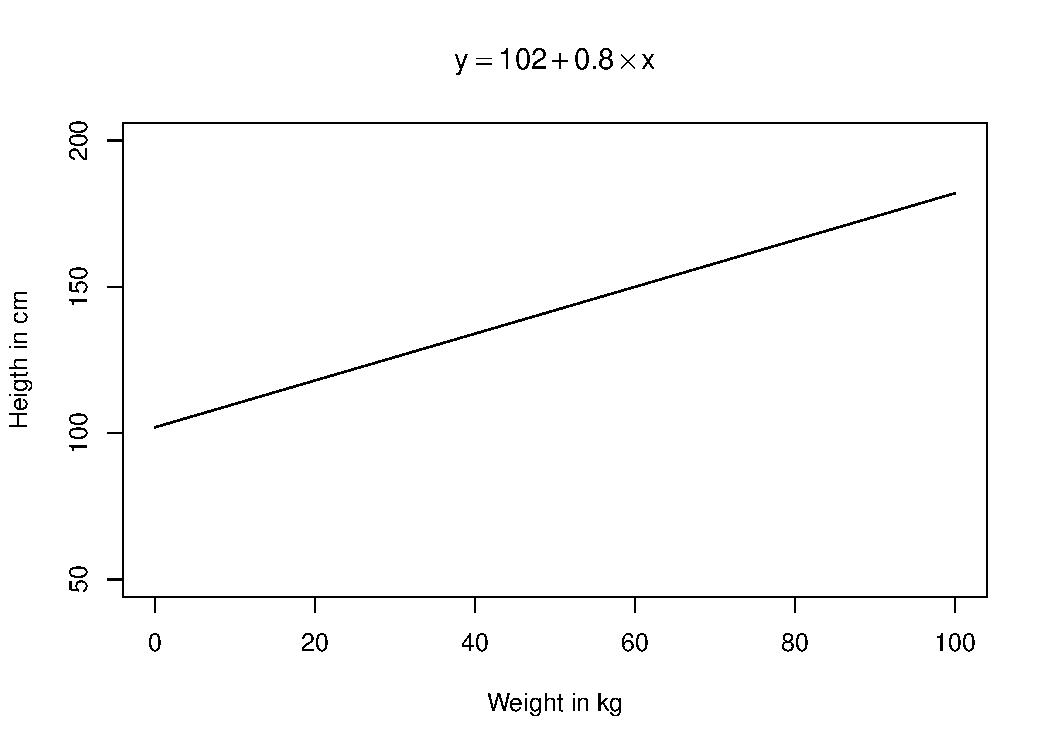
\includegraphics{05_lin_mudeli_laiendused_files/figure-latex/unnamed-chunk-13-1.pdf}

\subsection*{Mõjukuse plot}\label{mojukuse-plot}
\addcontentsline{toc}{subsection}{Mõjukuse plot}

\begin{itemize}
\tightlist
\item
  \emph{outlier}id -- studentideeritud residuaalid \textgreater{} 2 või
  \textless{} -2. Studentiseeritud residuaali saab (ligikaudu) jagades
  vaatluse residuaali residuaalide standardhälbega. See protseduur
  võimaldab paremini võrrelda erinevate vaatluste residuaale.
\end{itemize}

Standardiseeritud residuaali arvutamine: Kui \(E_i\) on i-s residuaal, k
on mudeli regressorite arv ja n on vaatluste arv, siis
\(h_i = 1/n + E_i/\sum~E^2\), \(S_E = (E^2/(n - k -1))^{1/2}\) ja
\(E_{st} = E_i/(S_E(1 - h_i)^{1/2})\) kus E\textasciitilde{}st on
standardiseeritud residuaal, mis suurtel valimitel on väga sarnane
studentiseeritud residuaaliga (mis erineb selle poolest, et välistab iga
residuaali S\textasciitilde{}E-st seda residuaali genereerinud
vaatluse). Kui n on suur, siis kehtib enam-vähem seos
\(E_{st} = E_i/sd(E)\), kus E\_st on nii standardiseeritud kui
studentiseeritud residuaal.

\begin{itemize}
\tightlist
\item
  \emph{high leverage} vaatlused -- hat \textgreater{} 1 - sugereerib
  \emph{high leverage} vaatlust Keskmine hat value = (k + 1)/n, kus k on
  regressorite arv (mitte arvestades intercepti) ja n on vaatluste arv.
  NB! Kuna \emph{high leverage} vaatlused tõmbavad regressioonijoon enda
  suunas, siis on neil sageli madalad residuaalid (erinevalt
  outlieritest, mis ei ole \emph{high leverage} vaatlused)
\end{itemize}

\begin{Shaded}
\begin{Highlighting}[]
\KeywordTok{library}\NormalTok{(car)}
\KeywordTok{influencePlot}\NormalTok{(m3, }\DataTypeTok{id.method=}\StringTok{"identify"}\NormalTok{, }\DataTypeTok{main=}\StringTok{"Influence Plot"}\NormalTok{,}
              \DataTypeTok{sub=}\StringTok{"Circle size is proportional to Cook's distance"}\NormalTok{)}
\end{Highlighting}
\end{Shaded}

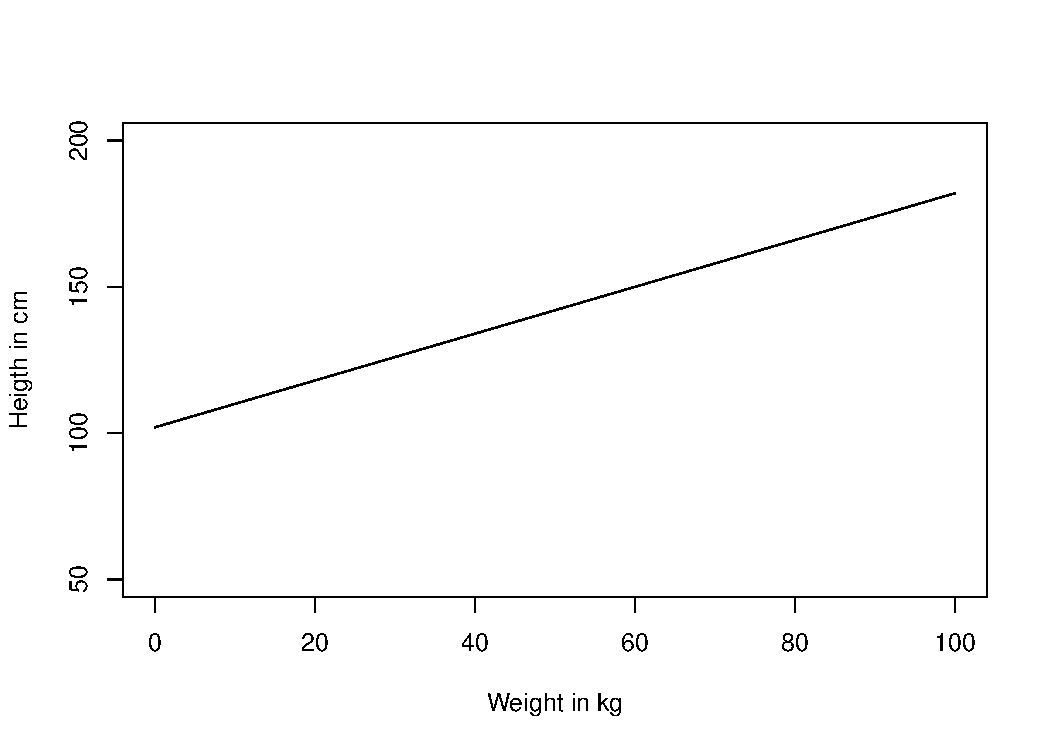
\includegraphics{05_lin_mudeli_laiendused_files/figure-latex/unnamed-chunk-14-1.pdf}

\begin{verbatim}
#>     StudRes    Hat   CookD
#> 15   -0.243 0.1236 0.00139
#> 42   -2.810 0.0621 0.08307
#> 69   -2.477 0.0253 0.02567
#> 107  -0.331 0.1638 0.00359
#> 119  -2.464 0.0824 0.08782
\end{verbatim}

Horisontaalsed referentsjooned näitavad 0, 2 ja -2 studentiseeritud
residuaale. Vertikaalsed referentsjooned näitavad hat-väärtusi 2h ja 3h.

\begin{quote}
Regressiooni \emph{outlier} on vaatlus, mille y-muutja väärtus on
ebatavaline X-muujutuja väärtuse kontekstis. Seega annab \emph{outlier}
mudeli fittimisel kõrge residuaaliga punkti. Lihtsalt
(mitte-konditsionaalselt) ebatavalised Y-i või X-i väärtused ei pruugi
olla \emph{outlier}id. Kui peaks juhuma, et \emph{outlier} langeb kokku
ebatavalise X-i väärtusega, siis selle punkti eemaldamine muudab
märkimisväärselt mudeli koefitsiente. Selline \emph{outlier} on ühtlasi
ka \emph{high leverage} vaatlus. Siit jõuame mõjukate vaatluste
(\emph{Influential observations}) defineerimisele --- Mõjukus mudeli
koefitsientidele = \emph{Leverage} x \emph{``outlierness''}. \emph{High
leverage} andmepunktid on x-muutujate ekstreemsed punktid, mille lähedal
ei ole n-mõõtmelises ruumis (kui teil on n x-muutujat) teisi punkte.
Seetõttu läheb fititud mudel just nende punktide lähedalt mõõda. Mõjukad
punktid on tüüpiliselt ka \emph{high leverage} punktid, kuid vastupidine
ei kehti!
\end{quote}

\subsubsection*{Cooki kaugus - mõjukus}\label{cooki-kaugus---mojukus}
\addcontentsline{toc}{subsubsection}{Cooki kaugus - mõjukus}

.cooksd on Cook-i kaugus, mis näitab mõjukust. Rusikareeglina tähendab
cooksd \textgreater{} 3 cooksd keskväärtust, et tegu võiks olla mõjuka
vaatlusega. Teine võimalus on pidada mõjukaks igat punkti, mis on kõrgem
kui 4/n. Kolmanadad arvavad jälle, et .cooksd \textgreater{} 1 v .cooksd
\textgreater{} 0.5 viitab mõjukale vaatlusele. Üldiselt on kõigi mudeli
eelduste kontrollidega nii, et vastava statistiku jaotuse jõllitamine on
sageli kasulikum kui automaatselt mingi \emph{cut-offi} järgi
talitamine.

Cooki D andmepunktile saame valemist
\(D_i = \frac{E'_i}{k+1} + \frac{h_i}{1-h_i}\), kus \(D_i\) on i-ndale
vaatlusele vastav Cooki kaugus ja \({E'_i}\) on sellele vaatlusele
vastav studentiseeritud residuaal.

\begin{Shaded}
\begin{Highlighting}[]
\KeywordTok{ggplot}\NormalTok{(}\DataTypeTok{data =} \OtherTok{NULL}\NormalTok{, }\KeywordTok{aes}\NormalTok{(}\DataTypeTok{x =} \DecValTok{1}\OperatorTok{:}\DecValTok{150}\NormalTok{, }\DataTypeTok{y =}\NormalTok{ a_m3}\OperatorTok{$}\StringTok{`}\DataTypeTok{.cooksd}\StringTok{`}\NormalTok{)) }\OperatorTok{+}\StringTok{ }\KeywordTok{geom_col}\NormalTok{() }\OperatorTok{+}\StringTok{ }
\StringTok{  }\KeywordTok{geom_hline}\NormalTok{(}\DataTypeTok{yintercept =} \DecValTok{4}\OperatorTok{/}\DecValTok{150}\NormalTok{)}\OperatorTok{+}\StringTok{ }
\StringTok{  }\KeywordTok{geom_hline}\NormalTok{(}\DataTypeTok{yintercept =} \DecValTok{3}\OperatorTok{*}\KeywordTok{mean}\NormalTok{(a_m3}\OperatorTok{$}\StringTok{`}\DataTypeTok{.cooksd}\StringTok{`}\NormalTok{), }\DataTypeTok{lty =} \DecValTok{2}\NormalTok{)}
\end{Highlighting}
\end{Shaded}

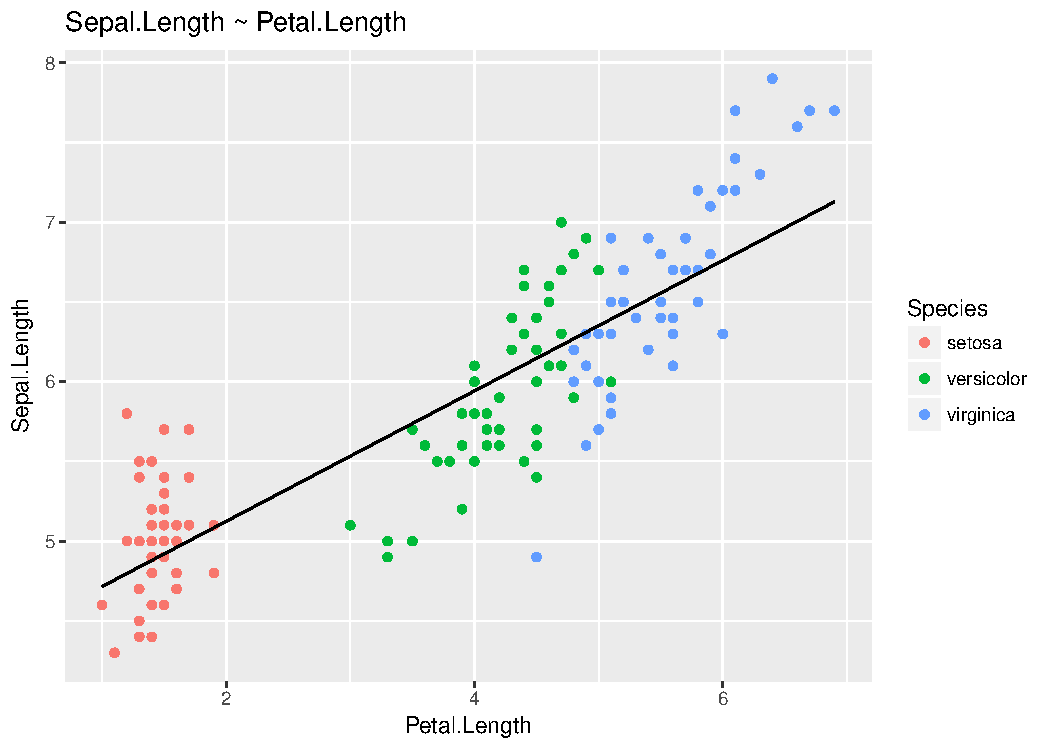
\includegraphics{05_lin_mudeli_laiendused_files/figure-latex/unnamed-chunk-15-1.pdf}

\subsection*{Residuaalide normaalsus - qq
plot}\label{residuaalide-normaalsus---qq-plot}
\addcontentsline{toc}{subsection}{Residuaalide normaalsus - qq plot}

Kas residuaalid on normaaljaotusega? NB! studentiseeritud residuaalid on
studenti t jaotusega ja üldiselt on targem vaadata neid, kui tavalisi
residuaale. Studenti t jaotusele pean ette andma ka vabadusastmete arvu
e df-i.

\begin{Shaded}
\begin{Highlighting}[]
\NormalTok{car}\OperatorTok{::}\KeywordTok{qqPlot}\NormalTok{(a_m3}\OperatorTok{$}\StringTok{`}\DataTypeTok{.std.resid}\StringTok{`}\NormalTok{, }\DataTypeTok{distribution =} \StringTok{"t"}\NormalTok{, }\DataTypeTok{df=}\DecValTok{149}\NormalTok{)}
\end{Highlighting}
\end{Shaded}

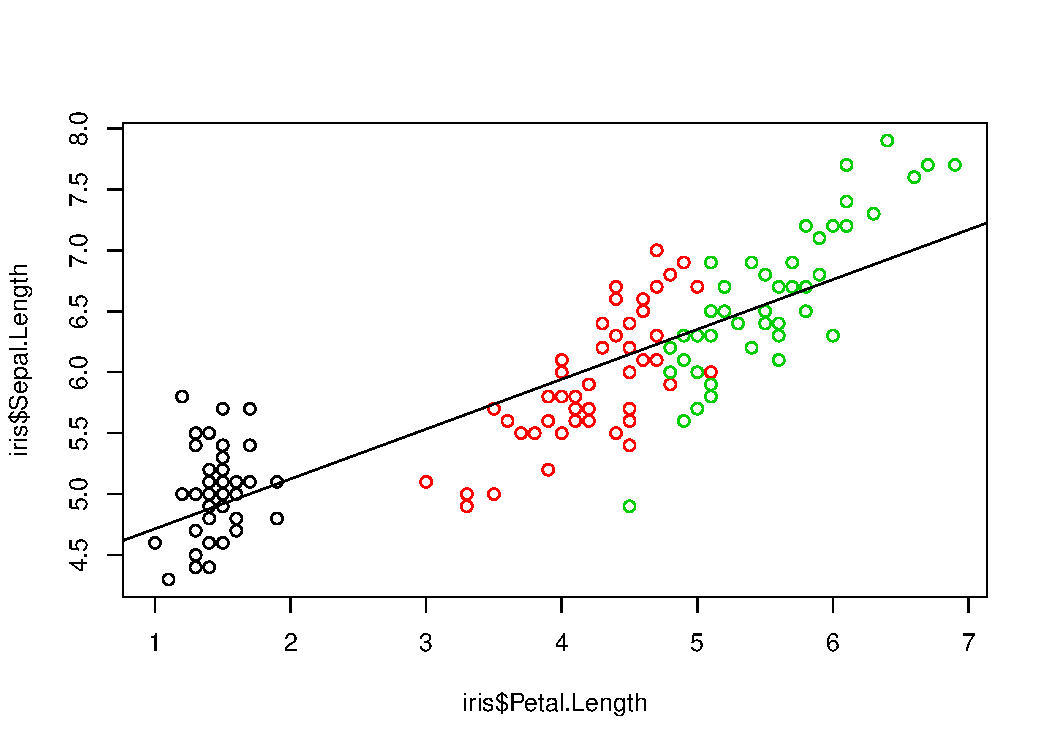
\includegraphics{05_lin_mudeli_laiendused_files/figure-latex/unnamed-chunk-16-1.pdf}

\begin{verbatim}
#> [1] 42 69
\end{verbatim}

QQ-plot näitab erinevust normaaljaotusest (t jaotusest) eelkõige
residuaalide jaotuse sabades. Antud juhul on kõik hästi.

Isegi oluisem on vaadata, et residuaalide jaotus ei oleks mitmetipuline.
Kui on, siis võib see olla märgiks, et mudelist on puudu mõni
faktormuutuja, mis andmetes olevad diskreetsed loomulikud
alampopulatsioonid lahku ajaks.

\begin{Shaded}
\begin{Highlighting}[]
\KeywordTok{ggplot}\NormalTok{(a_m3, }\KeywordTok{aes}\NormalTok{(}\StringTok{`}\DataTypeTok{.std.resid}\StringTok{`}\NormalTok{))}\OperatorTok{+}\StringTok{ }\KeywordTok{geom_density}\NormalTok{()}
\end{Highlighting}
\end{Shaded}

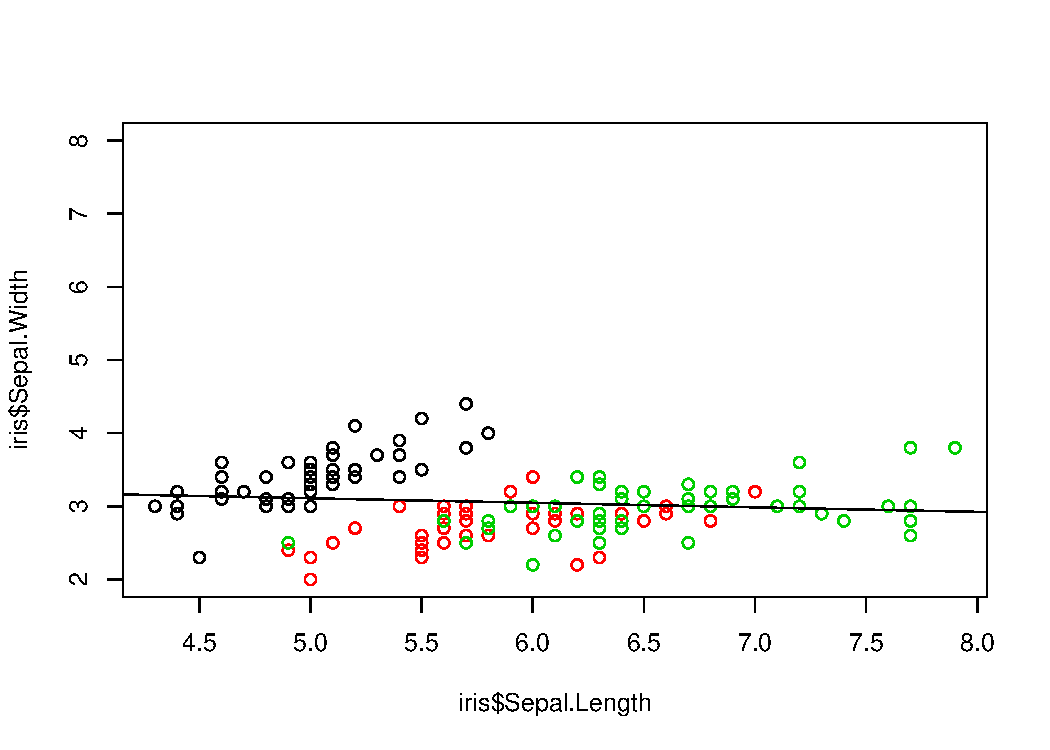
\includegraphics{05_lin_mudeli_laiendused_files/figure-latex/unnamed-chunk-17-1.pdf}

\subsection*{Homoskedastilisus - Scale-location
plot}\label{homoskedastilisus---scale-location-plot}
\addcontentsline{toc}{subsection}{Homoskedastilisus - Scale-location
plot}

Scale-location plot - homoskedastilisuse eeldust ehk seda, et
varieeruvus ei sõltuks prediktormuutuja väärtusest. Y-teljel on ruutjuur
studentiseeritud residuaalide absoluutväärtusest

\begin{Shaded}
\begin{Highlighting}[]
\KeywordTok{ggplot}\NormalTok{(a_m3, }\KeywordTok{aes}\NormalTok{(}\StringTok{`}\DataTypeTok{.fitted}\StringTok{`}\NormalTok{, }\StringTok{`}\DataTypeTok{.resid}\StringTok{`} \OperatorTok\StringTok{ }\NormalTok{abs }\OperatorTok\StringTok{ }\NormalTok{sqrt)) }\OperatorTok{+}\StringTok{ }
\StringTok{  }\KeywordTok{geom_point}\NormalTok{(}\KeywordTok{aes}\NormalTok{(}\DataTypeTok{color=}\NormalTok{Species), }\DataTypeTok{alpha=}\FloatTok{0.5}\NormalTok{) }\OperatorTok{+}\StringTok{ }
\StringTok{  }\KeywordTok{ylab}\NormalTok{(}\StringTok{"square root of absolute residual"}\NormalTok{)}\OperatorTok{+}
\StringTok{  }\KeywordTok{geom_smooth}\NormalTok{(}\DataTypeTok{se =} \OtherTok{FALSE}\NormalTok{)}
\end{Highlighting}
\end{Shaded}

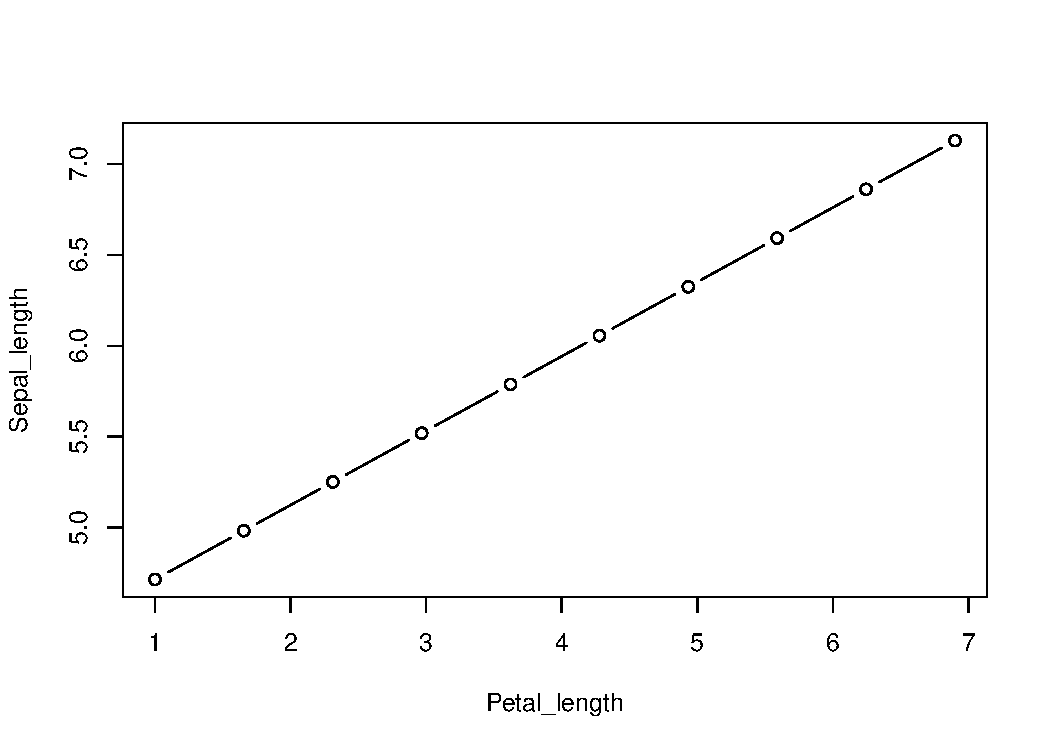
\includegraphics{05_lin_mudeli_laiendused_files/figure-latex/unnamed-chunk-18-1.pdf}

\section*{Residuaalid y ja x muutujate
vastu}\label{residuaalid-y-ja-x-muutujate-vastu}
\addcontentsline{toc}{section}{Residuaalid y ja x muutujate vastu}

Kõigepealt residuaalid y-muutja vastu

\begin{Shaded}
\begin{Highlighting}[]
\KeywordTok{ggplot}\NormalTok{(a_m3, }\KeywordTok{aes}\NormalTok{(Sepal.Width, }\StringTok{`}\DataTypeTok{.std.resid}\StringTok{`}\NormalTok{)) }\OperatorTok{+}\StringTok{ }\KeywordTok{geom_point}\NormalTok{(}\KeywordTok{aes}\NormalTok{(}\DataTypeTok{color=}\NormalTok{Species)) }\OperatorTok{+}\StringTok{ }\KeywordTok{geom_hline}\NormalTok{(}\DataTypeTok{yintercept =} \DecValTok{0}\NormalTok{, }\DataTypeTok{lty =}\DecValTok{2}\NormalTok{, }\DataTypeTok{color =}\StringTok{"darkgrey"}\NormalTok{) }\OperatorTok{+}\StringTok{ }
\StringTok{  }\KeywordTok{geom_smooth}\NormalTok{( }\DataTypeTok{se=}\NormalTok{F, }\DataTypeTok{color=}\StringTok{"black"}\NormalTok{, }\DataTypeTok{size=}\FloatTok{0.5}\NormalTok{)}
\end{Highlighting}
\end{Shaded}

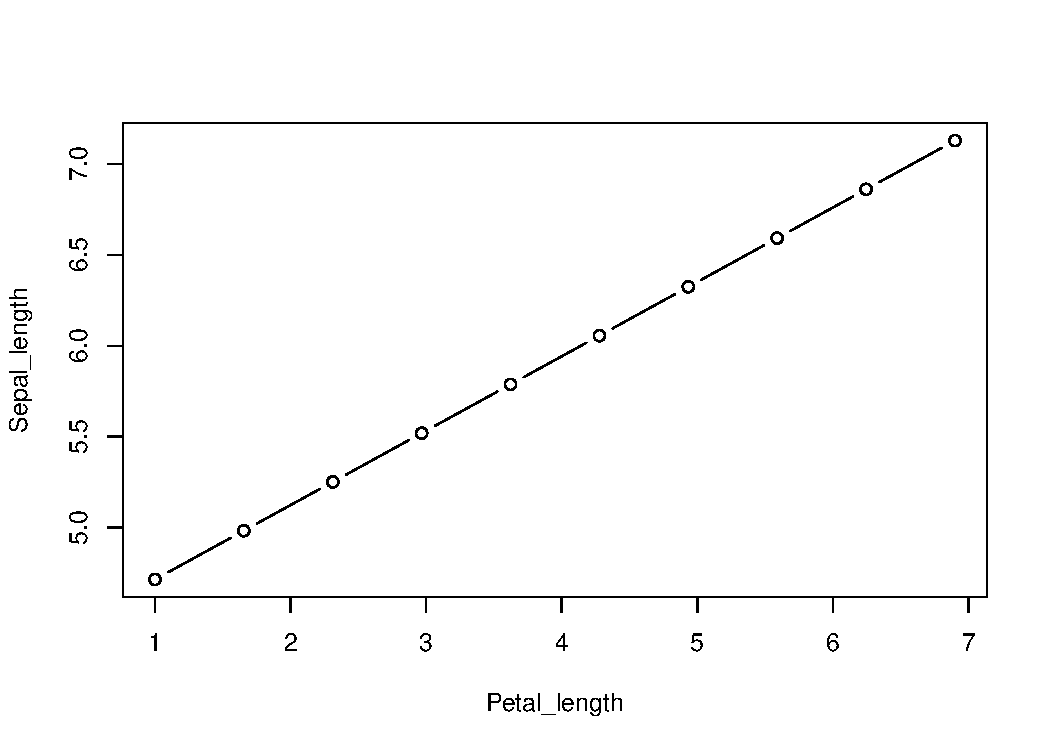
\includegraphics{05_lin_mudeli_laiendused_files/figure-latex/unnamed-chunk-19-1.pdf}

Mudel paistab süstemaatiliselt alahindama Sepal Width-i seal kus Sepal
Length on kõrge, ja vastupidi. Horisontaalne punktiirjoon näitab, kus
mudel vastab täpselt andmetele.

Studentiseeritud residuaalid sd ühikutes

Ja nüüd residuaalid x-muutuja vastu.

\begin{Shaded}
\begin{Highlighting}[]
\KeywordTok{ggplot}\NormalTok{(a_m3, }\KeywordTok{aes}\NormalTok{(Sepal.Length, }\StringTok{`}\DataTypeTok{.std.resid}\StringTok{`}\NormalTok{, }\DataTypeTok{color=}\NormalTok{Species)) }\OperatorTok{+}\StringTok{ }
\StringTok{  }\KeywordTok{geom_point}\NormalTok{() }\OperatorTok{+}
\StringTok{  }\KeywordTok{geom_hline}\NormalTok{(}\DataTypeTok{yintercept =} \DecValTok{0}\NormalTok{, }\DataTypeTok{lty =}\DecValTok{2}\NormalTok{, }\DataTypeTok{color =}\StringTok{"darkgrey"}\NormalTok{)}\OperatorTok{+}
\StringTok{  }\KeywordTok{geom_smooth}\NormalTok{(}\DataTypeTok{se=}\NormalTok{F, }\DataTypeTok{color=}\StringTok{"black"}\NormalTok{, }\DataTypeTok{size=}\FloatTok{0.5}\NormalTok{)}
\end{Highlighting}
\end{Shaded}

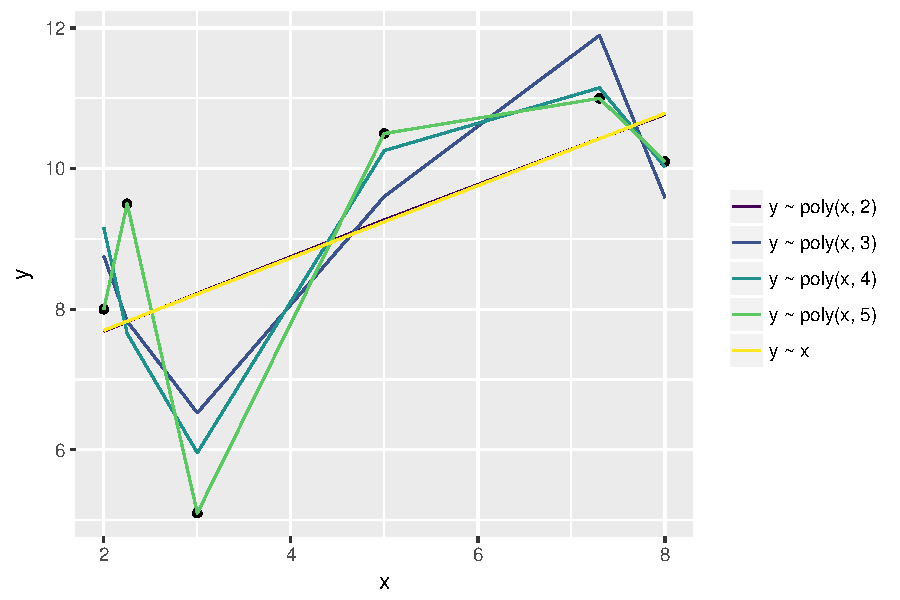
\includegraphics{05_lin_mudeli_laiendused_files/figure-latex/unnamed-chunk-20-1.pdf}
Ideaalsed residuaalid!

\section*{3. Teeme mudeli põhjal ennustusi (marginal
plots)}\label{teeme-mudeli-pohjal-ennustusi-marginal-plots}
\addcontentsline{toc}{section}{3. Teeme mudeli põhjal ennustusi
(marginal plots)}

Me ennustame y-i keskmisi väärtuseid etteantud x-i väärtustel.

ggpredict() ennustab y-muutuja väärtusi ühe x-muutuja väärtuste järgi,
hoides kõiki teisi x-muutujaid konstantsena.

Kõigepealt võrdleme lihtsa 1 prediktoriga mudeli ennustust kahe
prediktoriga mudeli ennustusega

\begin{Shaded}
\begin{Highlighting}[]
\NormalTok{lm1 <-}\StringTok{ }\KeywordTok{lm}\NormalTok{(Sepal.Width }\OperatorTok{~}\StringTok{ }\NormalTok{Sepal.Length, }\DataTypeTok{data =}\NormalTok{ iris)}
\NormalTok{lm2 <-}\StringTok{ }\KeywordTok{lm}\NormalTok{(Sepal.Width }\OperatorTok{~}\StringTok{ }\NormalTok{Sepal.Length }\OperatorTok{+}\StringTok{ }\NormalTok{Petal.Length, }\DataTypeTok{data =}\NormalTok{ iris)}

\NormalTok{mydf <-}\StringTok{ }\KeywordTok{ggpredict}\NormalTok{(lm1, }\DataTypeTok{terms =} \StringTok{"Sepal.Length"}\NormalTok{)}
\NormalTok{mydf2 <-}\StringTok{ }\KeywordTok{ggpredict}\NormalTok{(lm2, }\DataTypeTok{terms =} \StringTok{"Sepal.Length"}\NormalTok{)}

\KeywordTok{ggplot}\NormalTok{(mydf, }\KeywordTok{aes}\NormalTok{(x, predicted)) }\OperatorTok{+}\StringTok{ }
\StringTok{  }\KeywordTok{geom_line}\NormalTok{() }\OperatorTok{+}
\StringTok{  }\KeywordTok{geom_ribbon}\NormalTok{(}\DataTypeTok{data =}\NormalTok{ mydf, }\KeywordTok{aes}\NormalTok{(}\DataTypeTok{ymin =}\NormalTok{ conf.low, }\DataTypeTok{ymax =}\NormalTok{ conf.high), }
              \DataTypeTok{alpha =} \FloatTok{0.5}\NormalTok{, }\DataTypeTok{fill=}\StringTok{"lightgrey"}\NormalTok{) }\OperatorTok{+}
\StringTok{  }\KeywordTok{geom_line}\NormalTok{(}\DataTypeTok{data =}\NormalTok{ mydf2, }\KeywordTok{aes}\NormalTok{(x, predicted), }\DataTypeTok{lty=}\DecValTok{2}\NormalTok{)}\OperatorTok{+}
\StringTok{  }\KeywordTok{geom_ribbon}\NormalTok{(}\DataTypeTok{data =}\NormalTok{ mydf2, }\KeywordTok{aes}\NormalTok{(}\DataTypeTok{ymin =}\NormalTok{ conf.low, }\DataTypeTok{ymax =}\NormalTok{ conf.high), }
              \DataTypeTok{alpha =} \FloatTok{0.5}\NormalTok{, }\DataTypeTok{fill=}\StringTok{"lightgrey"}\NormalTok{) }\OperatorTok{+}
\StringTok{  }\KeywordTok{geom_point}\NormalTok{(}\DataTypeTok{data=}\NormalTok{iris, }\KeywordTok{aes}\NormalTok{(Sepal.Length, Sepal.Width, }\DataTypeTok{color=}\NormalTok{Species)) }\OperatorTok{+}\StringTok{ }
\StringTok{  }\KeywordTok{xlab}\NormalTok{(}\StringTok{"Sepal Length"}\NormalTok{) }\OperatorTok{+}\StringTok{ }
\StringTok{  }\KeywordTok{ylab}\NormalTok{(}\StringTok{"predicted sepal width"}\NormalTok{)}\OperatorTok{+}
\StringTok{  }\KeywordTok{theme_classic}\NormalTok{()}
\end{Highlighting}
\end{Shaded}

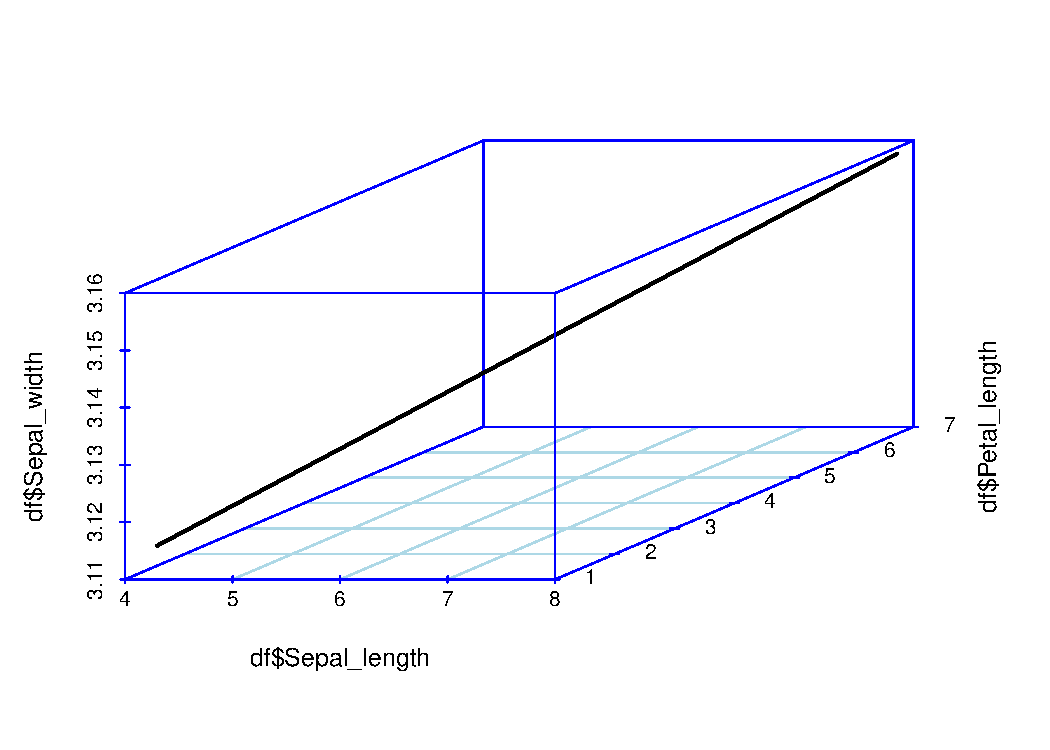
\includegraphics{05_lin_mudeli_laiendused_files/figure-latex/unnamed-chunk-21-1.pdf}

\begin{quote}
terms argument võtab kuni 3 muutujat, neist 2 peavad olema
faktormuutujad ja 3 muutuja korral tekib tabelisse veerg nimega facet,
mille abil saab tulemused facet\_wrap()-ga välja plottida.
\end{quote}

\begin{Shaded}
\begin{Highlighting}[]
\NormalTok{mydf <-}\StringTok{ }\KeywordTok{ggpredict}\NormalTok{(m3, }\DataTypeTok{terms =} \KeywordTok{c}\NormalTok{(}\StringTok{"Sepal.Length"}\NormalTok{, }\StringTok{"Species"}\NormalTok{))}
\KeywordTok{ggplot}\NormalTok{(mydf, }\KeywordTok{aes}\NormalTok{(x, predicted)) }\OperatorTok{+}\StringTok{ }
\StringTok{  }\KeywordTok{geom_line}\NormalTok{(}\KeywordTok{aes}\NormalTok{(}\DataTypeTok{color=}\NormalTok{group)) }\OperatorTok{+}\StringTok{ }
\StringTok{  }\KeywordTok{geom_point}\NormalTok{(}\DataTypeTok{data=}\NormalTok{iris, }\KeywordTok{aes}\NormalTok{(Sepal.Length, Sepal.Width, }\DataTypeTok{color=}\NormalTok{Species)) }\OperatorTok{+}\StringTok{ }
\StringTok{  }\KeywordTok{xlab}\NormalTok{(}\StringTok{"Sepal Length"}\NormalTok{) }\OperatorTok{+}
\StringTok{  }\KeywordTok{ylab}\NormalTok{(}\StringTok{"predicted sepal width"}\NormalTok{)}
\end{Highlighting}
\end{Shaded}

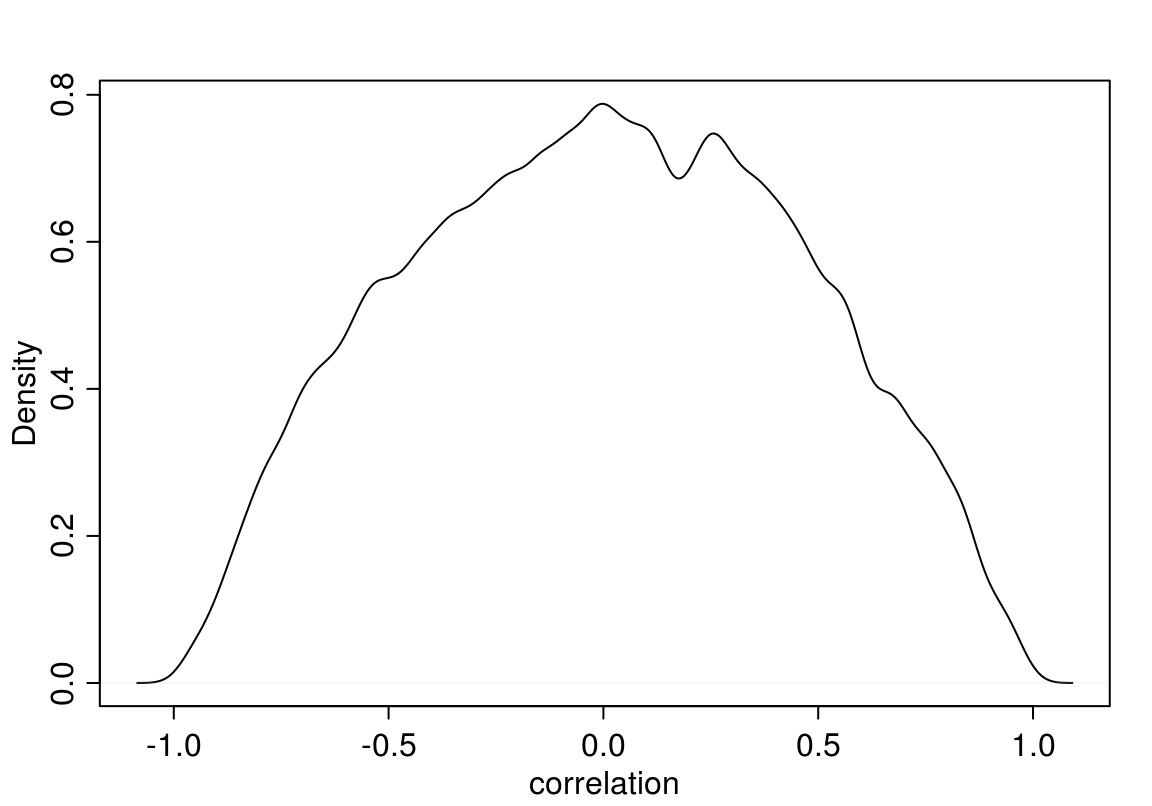
\includegraphics{05_lin_mudeli_laiendused_files/figure-latex/unnamed-chunk-22-1.pdf}

Nii saab sisestada üksikuid parameetriväärtusi ja neile ennustusi teha:

\begin{Shaded}
\begin{Highlighting}[]
\NormalTok{(mydf1 <-}\StringTok{ }\KeywordTok{ggpredict}\NormalTok{(m3, }\DataTypeTok{terms =} \KeywordTok{c}\NormalTok{(}\StringTok{"Sepal.Length [5, 22]"}\NormalTok{, }\StringTok{"Species [setosa, versicolor]"}\NormalTok{)))}
\CommentTok{#> }
\CommentTok{#> # Predicted values of Sepal.Width}
\CommentTok{#> # x = Sepal.Length}
\CommentTok{#> }
\CommentTok{#> # Species = setosa}
\CommentTok{#>   x predicted std.error conf.low conf.high}
\CommentTok{#>   5      3.42     0.039     3.35       3.5}
\CommentTok{#>  22     17.00     1.876    13.32      20.7}
\CommentTok{#> }
\CommentTok{#> # Species = versicolor}
\CommentTok{#>   x predicted std.error conf.low conf.high}
\CommentTok{#>   5      2.47      0.08     2.31      2.63}
\CommentTok{#>  22      7.91      1.21     5.53     10.28}
\end{Highlighting}
\end{Shaded}

\section*{4. Võrdleme mudeleid}\label{vordleme-mudeleid}
\addcontentsline{toc}{section}{4. Võrdleme mudeleid}

\begin{enumerate}
\def\labelenumi{\arabic{enumi}.}
\item
  Eeldus - kõik võrreldavad mudelid on fititud täpselt samade andmete
  peal.
\item
  Eeldus (ei ole vajalik AIC meetodi puhul) - tegemist on nn nested
  mudelitega. Nested mudel tähendab, et kõik väiksema mudeli liikmed on
  olemas ka suuremas mudelis.
\end{enumerate}

Mudelite võrdlus ANOVA-ga (ainult nested mudelid)

\begin{Shaded}
\begin{Highlighting}[]
\KeywordTok{tidy}\NormalTok{(}\KeywordTok{anova}\NormalTok{(lm1, lm2, m3))}
\CommentTok{#> Warning: Unknown or uninitialised column: 'term'.}
\CommentTok{#> # A tibble: 3 x 6}
\CommentTok{#>   res.df   rss    df sumsq statistic   p.value}
\CommentTok{#>    <dbl> <dbl> <dbl> <dbl>     <dbl>     <dbl>}
\CommentTok{#> 1    148  27.9    NA NA         NA   NA       }
\CommentTok{#> 2    147  15.4     1 12.5      169.   4.83e-26}
\CommentTok{#> 3    144  10.7     3  4.71      21.2  2.06e-11}
\end{Highlighting}
\end{Shaded}

Mudelite võrdlus AIC-ga

\begin{Shaded}
\begin{Highlighting}[]
\KeywordTok{AIC}\NormalTok{(lm1, lm2, m3)}
\CommentTok{#>     df   AIC}
\CommentTok{#> lm1  3 179.5}
\CommentTok{#> lm2  4  92.1}
\CommentTok{#> m3   7  43.3}
\end{Highlighting}
\end{Shaded}

AIC (Akaike Informatsiooni Kriteerium) on number, mis püüab tabada
mõistlikku tasakaalu mudeli fiti valimiandmetega ja parsinoomia vahel.
Väiksema AIC-ga mudel on eelistatud suurema AIC-ga mudeli ees (samas,
AIC-l kui ühel arvul puudub tõlgendus).

Probleem AIC-i taga on selles, et parem fit valimiandmetega võib
tähendada mudeli ülefittimist (ja seega halvemat mudelit). Kuna
ülefittimise tõenäosus kasvab koos mudeli keerukusega (parameetrite
arvuga), eelistame võimalikult lihtsat mudelit, mis samas seletaks
võimalikult suure osa valimiandmete varieeruvusest.

\chapter{Andmete transformeerimine}\label{andmete-transformeerimine}

Lineaarsed transformatsioonid võivad hõlbustada mudeli koefitsientide
tõlgendamist (näit. skaala millimeetritest meetritessse, tsentreerimine,
standardiseerimine). Mittelineaarsed transformatsioonid (logaritmimine,
jms) muudavad mudeli fitti ja võivad olla kasulikud mudeli
aditiivsuse/lineaarsuse parandamisel. Oluline on mõista, et
transformeeritud andmetega mudeleid tuleb tõlgendada transformeeritud
skaalas. Seega, kui algsel skaalal pole muud tõlgendust, kui et
väärtused on monotoonilised (näiteks suurem number on alati tähtsam kui
väiksem number), siis sobib meile sama hästi iga lineaarne
transformatsioon sellest skaalast (näiteks ruutjuure võtmine vms).
Bioloogias enamasti asjad nii lihtsad ei ole ja seetõttu keskendume siin
paremini tõlgendatavatele transformatsioonidele.

\section{Logaritmimine}\label{logaritmimine}

Kui muutujal saavad olla ainult positiivsed väärtused, siis on
logaritmimine vahest hea mõte. Enne logaritmima asumist paeb andmetest
kaotama ka nullid, näiteks asendades need mingi väikese positiivse
arvuga. Logaritmilises skaalas andmetele fititud mudelite \(\beta\)
koefitsiendid peaaegu alati \textless{} 1.

\subsection*{Miks ja millal muutujaid
logaritmida}\label{miks-ja-millal-muutujaid-logaritmida}
\addcontentsline{toc}{subsection}{Miks ja millal muutujaid logaritmida}

\begin{enumerate}
\def\labelenumi{\arabic{enumi}.}
\item
  Muutuja(te) logaritmimine muudab muutujate vahelised suhted
  mitte-lineaarseks, samas säilitades mudeli lineaarsuse. Ja vastupidi,
  kui tavalises meetrilises skaalas juhtuvad additiivse mudeli muutujate
  vahelised seosed olema mitte-lineaarsed, siis x-muutuja(te)
  logaritmimine võib need muuta lineaarseks, ja sellega päästa ühe
  olulisema lineaarse regressiooni eelduse (vt ka ptk 4.2).
\item
  Logarimimine on hea, kui soovite y ja x muutuja omavahelist sõltuvust
  tõlgendada üle suhtelise muutuse ehk muutuse protsendi. Kui algses
  skaalas on \(\beta\) koefitsiendi loomulik tõlgendus additiivne: x-i
  kasv 1 ühiku võrra ennustab y-i kasvu \(\beta\) ühiku võrra, siis
  naturaallogaritmitud x-i korral on üks loomulikest
  multiplikatiivsetest tõlgendustest: x-i kasv 1 ühiku võrra ennustab
  y-i muutust \ldots{} protsendi võrra. Additiivsel juhul me liidame ja
  lahutame, multiplikatiivsel juhul aga korrutame ja jagame.
\item
  Muutuja logaritmimine võib viia selle muutuja lähemale
  normaaljaotusele (lognormaaljaotuse logaritm on normaaljaotusega).
  Algselt paremale kaldu jaotuse äärmuspunktid võivad regressioonile
  liiga suurt kaalu omada, milline probleem sageli kaob logaritmimisel.
\item
  Kui mudeli residuaalid on ümber nulli tugevalt paremale poole kiivas
  jaotusega, siis andmete logaritmimine võib need normaliseerida. Samuti
  siis, kui residuaalide sd on proportsionaalne fititud väärtusega (st
  CV, mitte SD, on konstantne) ja siis, kui te ususte, et residuaalid
  peegeldavad multiplikatiivseid vigu.
\item
  Kui y ja x-i vaheline sõltuvus on eksponentsiaalne.
\item
  Y-muutuja logaritmimine võib aidata hetoroskedastilisuse vastu.
\item
  Teaduslik teooria võib indikeerida logaritmimist. Näit pH on log
  skaalas.
\item
  Logaritmimine võib lihtsustada mudelit, vähendades
  interaktsiooniliikmete arvu.
\end{enumerate}

Mudeli fiti kvaliteedi koha pealt pole vahet, millist logaritmi te
kasutate -- erinevused on ``pelgalt'' mudeli koefitsientide
tõlgendustes. Naturaallogaritmitud log(x) andmete peal fititud mudeli
korral on algses lineaarses skaalas tõlgendatav logaritmitud andmete
peal fititud \(\beta\), aga log-skaalas muutujate väärtused ei tähenda
peale vaadates suurt midagi. Vastupidiselt on kümnendlogaritmitud
log10(x) või kahendlogaritmitud log2(x) andmed log skaalas
tõlgendatavad, aga mitte neil fititud \(\beta\) lineaarses skaalas. Igal
juhul eelistavad loodusteadlased kasutada log2 ja log10 skaalasid, mida
on mugavam otse log-skaalas tõlgendada. log2 skaalas vastab üheühikuline
muutus kahekordsele muutusele algses skaalas ja anti-logaritm on
\(2^{log2(x)}\). Log10 skaalas vastab üheühikuline muutus 10-kordsele
muutusele algses skaalas ja anti-logaritm on \(10^{log10(x)}\).

\subsection*{Naturaallogaritmitud andmetega
töötamine}\label{naturaallogaritmitud-andmetega-tootamine}
\addcontentsline{toc}{subsection}{Naturaallogaritmitud andmetega
töötamine}

Järgnevalt õpetame naturaallogaritmitud andmetega fititud mudelite
\(\beta\) koefitsiendite tõlgendamist algses, meetrilises skaalas ja
suhtelises protsendiskaalas.

Naturaallogaritmi alus on \(e \approx 2.71828\) ja sellel on järgmised
matemaatilised omadused:

\begin{enumerate}
\def\labelenumi{\arabic{enumi}.}
\item
  \(log(e) = 1\)
\item
  \(log(1) = 0\)
\item
  \(log(A^r) = r * log(A)\)
\item
  \(e^{log(A)} = A\) ehk \(exp(log(A)) = A\) ehk
  \(2.72^{log(A)} \approx A\)
\item
  \(log(AB)=logA + logB\)
\item
  \(log(A/B)=logA - logB\)
\item
  \(exp(AB) = exp(A)^B\)
\item
  \(exp(A+B) = exp(A)exp(B)\)
\item
  \(exp(A-B) = exp(A)/exp(B)\)
\end{enumerate}

Lineaarsel regressioonil saab log-transformatsiooni kasutada kolmel
erineval viisil:

\begin{itemize}
\item
  y = \(\alpha\) + \(\beta\)x --- lineaarne mudel (transformeerimata)
\item
  y = \(\alpha\) + \(\beta\) * log(x) --- lineaar-log mudel
  (transformeeritud on prediktor(id))
\item
  log(y) = \(\alpha\) + \(\beta\)x -- log-lineaar mudel
  (transformeeritud on y-muutuja)
\item
  log(y) = \(\alpha\) + \(\beta\) * log(x) -- log-log mudel
  (transformeeritud on y ja x muutujad)
\end{itemize}

\textbf{Lineaarses} mudelis y = \(\alpha\) + \(\beta\)x, annab \(\beta\)
selle, mitu ühikut muutub Y keskväärtus, kui X muutub ühe ühiku võrra.

\textbf{Lineaar-log} mudelis jääb kehtima sama \(\beta\) tõlgendus, mis
ülalpool, ainult et log-ühikutes. Seega viib logx-i muutus ühe log ühiku
võrra y keskväärtuse muutusele \(\beta\) ühiku võrra (see kehtib muidugi
ka log2 ja log10 skaalades).

Kui me juba kasutasime naturaallogaritmimist, siis tahame ilmselt
tõlgendust pigem muutuse protsendina ja/või algsetes meetrilistes
skaalas (log2 ja log10 ei võimalda selliseid mugavaid tõlgendusi):

\begin{itemize}
\item
  \(\beta\) on oodatud y muutus, kui x kasvab \(ex\) korda.
\item
  Kui \(\beta\) on väike, siis saab seda tõlgendada kui suhtelist
  erinevust. Näiteks, kui \(\beta\) = 0.06, siis 1 ühikuline x-i muutus
  viib u 6\%-sele y muutusele. Sedamõõda kuidas \(\beta\) kaugeneb
  nullist (näiteks \(\beta\) = 0.4), hakkab selline hinnang tõsiselt
  alahindama tegelikku x-i mõju y väärtusele.
\item
  Oodatud y muutus kui x kasvab p protsenti on \(\beta\) * log({[}100 +
  p{]}/100). Näit, kui x kasvab 10\% võrra (ehk kui korrutame x-i
  1.1-ga), siis log(110/100) = 0.095 ja 0.095\(\beta\) on oodatud y
  muutus.
\end{itemize}

\textbf{Log-lineaarse} mudeli korral,

\begin{itemize}
\item
  kui x kasvab 1 ühiku võrra, siis oodatud y väärtus kasvab
  exp(\(\beta\)) korda.
\item
  Kui x kasvab c ühiku võrra, siis oodatud y väärtus kasvab
  exp(c\(\beta\)) korda.
\item
  Kui \(\beta\) on väike, siis 100 * \(\beta\) vastab y protsentuaalsele
  muutusele juhul kui x muutub 1 ühiku võrra (kui \(\beta\) = 0.06, siis
  x-i muutus 1 ühiku võrra viib y-i 6\% tõusule).
\end{itemize}

\textbf{Log-log} mudeli korral on tõlgendus oodatud y-i muutus
protsentides kui x muutub mingi protsendi võrra. Sellist suhet
kotsutakse ökonomeetrias elastiliseks ja log x-i \(\beta\) koefitsient
on ``elastilisus.''

\begin{itemize}
\item
  Kui me korrutame x-i e-ga, siis korrutame oodatud y-i väärtuse
  exp(\(\beta\))-ga.
\item
  Et saada y suhtelist muutust, kui x kasvab p protsenti, arvuta a =
  log({[}100 + p{]}/100) ja siis võta exp(a\(\beta\)).
\end{itemize}

\section{Standardiseerimine}\label{standardiseerimine}

Kui prediktor \(x_1\) on mõõdetud näiteks eurodes ja prediktor \(x_2\)
aastates, siis on meil fititud koefitsientidele \(b_1\) ja \(b_2\) peale
vaadates raske öelda, kumb mõjutab y-muutuja väärtust rohkem. Kuna euro
ühik on palju granuleeritum kui aasta, siis võib ka väga väike nullist
erinev \(b_1\) omada mudeli seisukohast suuremat tähtsust kui
suhteliselt suur \(b_2\).

\(x.z = (x - mean(x))/sd(x)\)

Sellisel viisil standardiseeritud andmete keskväärtus on 0 ja sd = 1.
Seega on kõik predikorid samas skaalas ja me mõõdame efekte sd ühikutes.
See lubab võrrelda algselt erinevas skaalas prediktoreid. Intecept
tähendab nüüd keskmist ennustust, juhul kui kõik prediktorid on
fikseeritud oma keskväärtustel.

Kui mudel sisaldab lisaks pidevatele prediktoritele ka binaarseid
prediktoreid, siis on kasulikum standardiseerida üle 2xSD, jättes
binaarsed muutujad muutmata.

\(x.z2 = (x - mean(x))/(2 * sd(x))\)

Nüüd tähendab 1 ühikuline muutus efekti -1 SD-st kuni 1 SD-ni üle
keskväärtuse.

\subsection*{Korrelatsioon üle regressiooni ja regressioon
keskmisele}\label{korrelatsioon-ule-regressiooni-ja-regressioon-keskmisele}
\addcontentsline{toc}{subsection}{Korrelatsioon üle regressiooni ja
regressioon keskmisele}

Kui standardiseerime nii y kui x-i

\texttt{x\ \textless{}-\ (x\ -\ mean(x))\ /\ sd(x)}
\texttt{y\ \textless{}-\ (y\ \ -mean(y))\ /\ sd(y)}

siis y\textasciitilde{}x regressiooni intercept = 0 ja tõus on sama, mis
x ja y vaheline korrelatsioonikoefitsient r. Seega jääb tõus alati -1 ja
1 vahele.

Siit tuleb ka seletus nähtusele, mida kutsutakse regressiooniks
keskmisele (\emph{regression to the mean}). Fakti, et y on sellises
mudelis alati 0-le lähemal kui x, kutsutaksegi regressiooniks
keskmisele. Näiteks, kui olete 20 cm keskmisest pikem ja pikkuse
päritavus on 0.5, siis on oodata, et teie järglased on keskeltläbi 10 cm
võrra keskmisest pikemad (ja teist lühemad). Selle pseudo-põhjusliku
nähtuse avastas Francis Galton.

\section{Tsentreerimine}\label{tsentreerimine}

x.c1 = x - mean(x) annab keskväärtuseks nulli aga jätab varieeruvused
algsesse skaalasse. Näiteks interaktsioonimudelite koefitsiendid on otse
tõlgendatavad tsentreeritud prediktorite korral.

Teine võimalus on tsentreerida mõnele teaduslikult mõistlikule
väärtusele. Näiteks IQ-d saab tsentreerida 100-le (x - 100).

\section{Mudeli koefitsientide
transformeerimine}\label{mudeli-koefitsientide-transformeerimine}

Ilma interaktsioonideta mudeli korral saab sama tulemuse, mis
prediktoreid tsentreerides, kui me reskaleerime tavalises skaalas
fititud mudeli koefitsiendid, korrutades iga \(\beta\) oma prediktori
kahekordse sd-ga (\(\beta_x = \beta \times 2 \times sd(x)\)). Nende
\(\beta_x\)-de pealt näeb iga muutuja suhtelist tähtsust mudelis.

Teine võimalus beta koefitsientide transformeerimiseks, mis ei eelda
prediktorite normaalsust, on korrutada betad läbi vastavate muutujate
interkvartiilsete range-dega (IQR).

Hoitatus: standardiseeritud koefitsiente ei tohi kasutada, et võrrelda
samade prediktorite mõju erinevate andmete peal fititud sama
struktuuriga mudelile.

\section{Pidev või diskreetne
muutuja?}\label{pidev-voi-diskreetne-muutuja}

Tavaliselt on mõistlik fittida mudel pidevale y muutujale ka siis, kui
tahame lõpuks tõlgenada tulemusi diskreetsel skaalal. Pidev muutuja
sisaldab rohkem informatsiooni ja seetõttu on meil lootust saada parem
fit. Erandiks on sellised pidevad x muutujad, mille mõju y-le on
mittelineaarne (näiteks vanuse mõju suremusele). Siin on vahest mõistlik
konverteerida pidev muutuja faktormuutujaks ja saada hinnang näiteks
igale vanuseklassile eraldi.

Additiivne mudel eeldab, et emaste ja isaste tõusud on võrdsed, mistõttu
need fititakse sama beta koefitsiendiga, mis tähendab, et
x\textsubscript{2} mõju pidelvale prediktorile x\textsubscript{1} on, et
me saame mudeli ennustusena faktori n tasemele vastavad n paralleelset
sirget, millest igaüks näitab pideva x\textsubscript{1} seost pideva
y-ga erinevatel x\textsubscript{2} tasemetel. 0/1 kodeeringus
regressorite interceptid annavad nende paralleelsete sirgete vahelised
kaugused üldise-intercepti poolt antud faktori taseme ennustusest.

\section{mitmese regressiooni üldised
printsiibid}\label{mitmese-regressiooni-uldised-printsiibid}

\begin{enumerate}
\def\labelenumi{\arabic{enumi}.}
\item
  võta sisse kõik teaduslikku huvi pakkuvad muutujad ja viska välja
  muutujad, mille kohta sul pole põhust arvata, et nad võiksid y
  väärtusi mõjutada.
\item
  kontrolli, ega muutujate vahel ei esine väga tugevaid korrelatsioone
  (kollineaarsus). Kui jah, siis kombineeri kollineaarsed muutujad üheks
  või transformeeri neid või viska mõni muutuja välja.
\item
  muutujad, mis ei varieeru, ei oma ka regressioonis mõju.
\item
  tugeva mõjuga muutujate puhul võib olla vajalik sisse tuua nende
  muutujate interkatsioond (vt ptk \ldots{}).
\item
  muutujad, mida sa reaalselt mõõtsid, ei pruugi olla need muutujad, mis
  mudelisse lähevad -- näiteks arvuta kehamassiindeks mõõdetud muutujate
  põhjal.
\item
  kui pidevad prediktorid transformeerida log skaalasse, siis on
  lineaarsesse mudelisse pandud efektid multiplikatiivsed, mitte
  aditiivsed.
\end{enumerate}

\chapter{Veamudel}\label{veamudel}

\begin{Shaded}
\begin{Highlighting}[]
\KeywordTok{library}\NormalTok{(tidyverse)}
\KeywordTok{library}\NormalTok{(brms)}
\KeywordTok{library}\NormalTok{(broom)}
\end{Highlighting}
\end{Shaded}

\section{Lihtne varieeruvuse mudel}\label{lihtne-varieeruvuse-mudel}

Oletame, et me oleme mõõtnud nelja patsienti ja saanud tulemuseks 1.2,
2.12, 1.4 ja 8.34. Kuidas me oma valimit iseloomustame ja kas me
peaksime 4. tulemuse, kui kahtlase, välja viskama? Arvatavasti tahaksime
saada hinnangut kõige tõenäolisemale mõõtetulemusele patsientide
populatsioonis ehk siis keskmise või tüüpilise patsiendi väärtusele. Ja
lisaks ka hinnangut patsientide vahelise varieeruvuse määrale. Meid võib
ka huvitada võrrelda patsientide ja tervete inimeste varieeruvust.
Esmapilgul tundub see lihtsa ülesandena, mis ei vaja mudeldamist --
lihtsalt arvutame aritmeetilise keskmise ja standardhälbe ja meil on
mõlemad hinnangud olemas. Aga tegelikult oleme probleemi ees, millele
pole ühte õiget lahendust.

Kui me viskame 4. tulemuse välja, siis tuleb meie keskmine kuhugi 1.5
kanti, muidu aga piirkonda, mille lähedal meil ei ole ühtegi
andmepunkti. Samuti annaks sd arvutus üsna erinevad tulemused. Kumb
võimalus siis valida? Selleks peame ikkagi otsustama, kuidas
modelleerida oma andmed. Sõltuvalt looduslikust protsessist, mis need
andmed genereeris, võiks andmete mudel olla näiteks normaaljaotus,
lognormaaljaotus vms. Kui valime normaaljaotuse, millise õlad langevad
väga kiiresti, siis on vaid väike tõenäosus kohata tervelt veerandit oma
andmepunktidest nõnda kaugel teistest, mis annab argumendi selle punkti
eemaldamiseks. Aga lognormaaljaotuse korral, mille õlg laskub palju
aeglasemalt, on tõenäosus 4. mõõtmisest isegi kaugemal olevaid andmeid
kohata palju suurem ja seega peaksime selle andmepunkti sisse jätma.
Erinevat tüüpi mudelitel on erinevad parameetrid, millele saab andmete
põhjal väärtusi otsida. See, et normaaljaotuse parameetrit \(\mu\) saab
meie näites arvutada aritmeetilise keskmise kaudu, ei tähenda, et ka
teiste mudelite korral peaksime sama lokatsiooniparameetrit fittima (või
et neil mudelitel üldse oleks lokatsiooniparameeter). Sarnased lood on
muidugi ka varieeruvust iseloomustava parameetriga.

Statistilist mudelit saab kasutada mitmel moel.

\begin{enumerate}
\def\labelenumi{\arabic{enumi}.}
\item
  Mudel toob sisse lisainformatsiooni andmete jaotuse kuju kohta, mida
  valimiandmetes endis ei pruugi sisalduda, ja mis tõstab meie
  järelduste kvaliteeti (või langetab seda, kui valisime kehva mudeli).
\item
  Võrreldes erinevat tüüpi mudelite sobivust andmetega ning omades aimu
  protsesside kohta, mida üks või teine mudel võiks adekvaatselt
  kirjeldada, on võimalik teha järeldusi loodusliku mehhanismi kohta,
  mis genereeris andmed, mille põhjal mudelid fititi.
\item
  Me võime fititud mudeli põhjal teha ennustusi, ehk genereerida uusi
  andmeid \emph{in silico}.
\end{enumerate}

Niisiis lihtne mudel andmetele: \(\mu\) ehk aritmeetiline keskmine kui
hinnang kõige tõenäosemale väärtusele. See on deterministlik nn
\emph{protsessimudel}, kus samad valimiväärtused annavad alati sama ja
ühese tulemuse. Statistiline mudel sisaldab endas nii protsessimudelit
kui tõenäosuslikku nn \emph{varieeruvuse mudelit} (ajaloolistel
põhjustel kutsutakse seda sageli veamudeliks), mis tuleb sisse
tõenäosusjaotuse kujul

\[dnorm(\mu, \sigma)\]

Selle mudeli on võimalik ümber sõnastada (seda seeläbi üldistades)
lihtsa regressioonivõrrandina \(y = b_0\), kusjuures \(\mu = b_0\) ehk
andmete keskväärtus võrdub regressioonisirge interceptiga. Asendades
saame

\[y \sim dnorm(b_0, \sigma)\]

Tilde \(\sim\) tähistab seose tõenäosuslikkust, ehk seda, et y muutuja
ennustuslikd väärtused tõmmatakse juhuvalimina normaaljaotusest, mis
omakorda on fititud empiiriliste väärtuste (ehk valimi) põhjal.

Seega on meil normaaljaotuse keskväärtus võimalik leida aritmeetilise
keskmisena või samaväärselt vähimruutude meetodiga, mis paneb
keskväärtuse kohta, kus keskväärtuse ja iga andmepunkti vahelise
kauguste ruutude summa tuleb minimaalne. Vähimruutude meetod on üldisem,
sest töötab ka järgmises peatükis, kus me asendame \(\mu\) terve
regressioonivõrrandiga kujul
\(y = b_0 + b_1x_1 + b_2x_2 + ... + b_ix_i\) (protsessimudel). Ja kui
meie regressioonivõrrandid lähevad mittelineaarseks ja vähimruutude
meetod nende fittimisel enam ei tööta, siis veel üldisem meetod, Bayesi
teoreem, töötab ikka.

Kuigi aritmeetiline keskmine ja vähimruutude meetod annavad sama
hinnangu lokatsiooniparameetrile, ei ütle need midagi sigma kohta. Samas
Bayesi meetod annab hinnangu (koos usaldusintervalliga) mõlemale
parameetrile.

\begin{verbatim}
Normaaljaotus mudeldab lokalisatsiooniparameetrit mu populatsiooni 
tüüpilise või keskmise liikme hinnanguna ja varieeruvusparameetrit 
sigma populatsiooni liikmete vaheliste erinevuste määra hinnanguna. 
\end{verbatim}

Arvutame lihtsa mudeli läbi vähimruutude meetodiga ja Bayesi meetodiga

\begin{Shaded}
\begin{Highlighting}[]
\KeywordTok{set.seed}\NormalTok{(}\DecValTok{1234321}\NormalTok{)}
\NormalTok{andmed <-}\StringTok{ }\KeywordTok{tibble}\NormalTok{(}\DataTypeTok{a=} \KeywordTok{rnorm}\NormalTok{(}\DecValTok{4}\NormalTok{))}
\KeywordTok{plot}\NormalTok{(andmed)}
\end{Highlighting}
\end{Shaded}

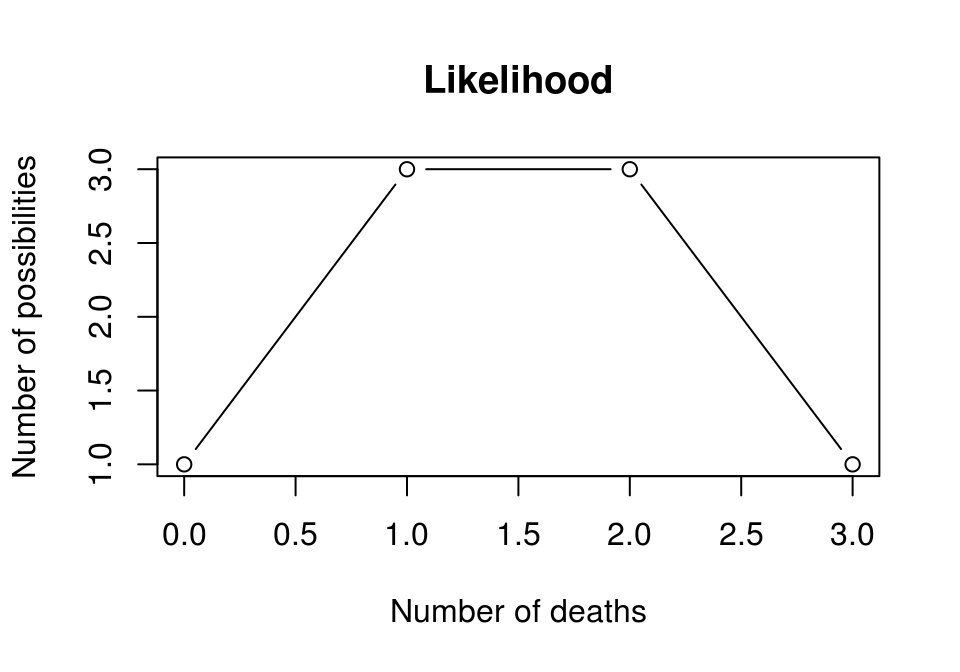
\includegraphics{06_veamudel_files/figure-latex/unnamed-chunk-3-1.pdf}

\begin{Shaded}
\begin{Highlighting}[]
\KeywordTok{mean}\NormalTok{(andmed}\OperatorTok{$}\NormalTok{a); }\KeywordTok{sd}\NormalTok{(andmed}\OperatorTok{$}\NormalTok{a)}
\CommentTok{#> [1] 1.24}
\CommentTok{#> [1] 0.662}
\end{Highlighting}
\end{Shaded}

Vähimruutude meetodit rakendab lm() funktsioon

\begin{Shaded}
\begin{Highlighting}[]
\KeywordTok{lm}\NormalTok{(a}\OperatorTok{~}\DecValTok{1}\NormalTok{, }\DataTypeTok{data =}\NormalTok{ andmed) }\OperatorTok\StringTok{ }\NormalTok{broom}\OperatorTok{::}\KeywordTok{tidy}\NormalTok{()}
\CommentTok{#> # A tibble: 1 x 5}
\CommentTok{#>   term        estimate std.error statistic p.value}
\CommentTok{#>   <chr>          <dbl>     <dbl>     <dbl>   <dbl>}
\CommentTok{#> 1 (Intercept)     1.24     0.331      3.74  0.0333}
\end{Highlighting}
\end{Shaded}

Ja Bayesi brms::brm()

\begin{Shaded}
\begin{Highlighting}[]
\NormalTok{(Bayes_mudel <-}\StringTok{ }\KeywordTok{brm}\NormalTok{(a}\OperatorTok{~}\DecValTok{1}\NormalTok{, }\DataTypeTok{data =}\NormalTok{ andmed) }\OperatorTok\StringTok{ }\NormalTok{broom}\OperatorTok{::}\KeywordTok{tidy}\NormalTok{())}
\end{Highlighting}
\end{Shaded}

\begin{verbatim}
#> # A tibble: 2 x 5
#>   term        estimate std.error lower upper
#>   <chr>          <dbl>     <dbl> <dbl> <dbl>
#> 1 b_Intercept     1.24     0.684 0.196  2.25
#> 2 sigma           1.27     1.24  0.461  3.02
\end{verbatim}

Nagu näete, lm() fitib ainult mu parameetri, samas kui me Bayesi
meetodit kasutades saame hinnangu (koos usalduspiiridega) kahele
parameetrile: mu ehk intercept ja sigma ehk sd.

Meie poolt simuleeritud andmed tulevad normaaljaotusega populatsioonist,
mille mu = 0 ja sd = 1. Kumbki meetod ei luba meile null-intercepti sest
andmeid on vähe ja need on juhusliku valimivea tõttu kallutatud.
See-eest sigma hinnang, mille Bayes meile annab on küll laiavõitu (ikka
sellepärast, et meil on vähe andmeid), aga vähemalt hõlmab endas õiget
väärtust.

\section{protsessimudel ja varieeruvuse mudel lineaarses
regressioonis}\label{protsessimudel-ja-varieeruvuse-mudel-lineaarses-regressioonis}

Kui mudel \(kaal = b_0 + b_1 ~pikkus\) ennustab, et 160 cm inimene
kaalub keskmiselt 80 kg, siis protsessi mudel ei ütle, kui suurt
pikkusest sõltumatut kaalude varieeruvust võime oodata 160 cm-ste
inimeste hulgas. Selle hinnangu andmiseks tuleb mudelile lisada
varieeruvusekomponent, sageli normaaljaotuse kujul, mis modelleerib
üksikute inimeste kaalude varieeruvust (mitte keskmise kaalu
varieeruvust) igal mõeldaval ja mittemõeldaval pikkusel.

\begin{quote}
Bioloogid, erinevalt füüsikutest, usuvad, et valimisisene andmete
varieeruvus on tingitud pigem bioloogilisest varieeruvusest kui
mõõtmisveast, aga loomulikult sisaldub selles ka mõõtmisviga.
\end{quote}

Kuidas varieeruvuskomponent lineaarsesse mudelisse sisse tuua? Ilma
varieeruvuskomponendita mudel:

\[y = b_0 + bx\]

ennustab y-i keskväärtust erinevatel x-i väärtustel.

Varieeruvuskomponent:

\[y\sim dnorm(\mu,~\sigma)\]

kus \(\mu\) (\emph{mu}) on mudeli poolt ennustatud keskväärtus ja
\(\sigma\) (sigma) on mudeli poolt ennustatud standardhälve ehk
varieeruvus andmepunktide tasemel. Varieeruvusmudelis on keskväärtuse
ehk \emph{mu} ennustus endiselt deterministlik ja sigma töötab
originaalsel andmetasemel, mitte keskväärtuste tasemel. See võimaldab
protsessimudeli varieeruvusmudelisse sisse kirjutada lihtsalt \emph{mu}
ümber defineerides:

\[\mu = b_0 + bx\]

mis tähendab, et

\[y \sim dnorm(b_0 + b_1x, ~\sigma)\]

See ongi sirge mudel koos varieeruvuskomponendiga. Seega on sellel
lineaarsel regressioonimudelil kolm parameetrit: intercept \(b_0\), tõus
\(b_1\) ja ``veaparameeter'' \(\sigma\). Sellist mudelit on mõistlik
fittida Bayesi teoreemi abil. Bayesi meetodiga fititud mudel, mida
kutsutakse posteerioriks, näitab, millised kombinatsioonid nendest
kolmest parameetrist usutavalt koos esinevad, ja millised mitte. Seega
on fititud 3 parameetriga bayesi mudel 3-dimensionaalne tõenäosusjaotus
(3D posteerior). Muidugi saame ka ükshaaval välja plottida kolm 1D
posteeriori, millest igaüks iseloomustab üht parameetrit ning on
kollapseeritud üle kahe ülejäänud parameetri. \href{pidev}{Edaspidi}
õpime selliste mudelitega töötama.

\begin{quote}
Kõik statistilised mudelid on tõenäosusmudelid ning sisaldavad
varieeruvuskomponenti.
\end{quote}

Kuna erinevalt lokatsiooniparameetrist, ei aja me mudelis sigmat lahku
vastavalt x-i väärtustele, siis meie varieeruvusmudel (ja enamus
veamudeleid, millega me edaspidi töötame) modelleerib igale x-i
väärtusele (kaalule) sama suure y-i suunalise varieeruvuse (pikkuste
sd). Suurem osa statistikast kasutab eeldusi, mida keegi päriselt tõe
pähe ei võta, aga millega on arvutuslikus mõttes lihtsam elada. Siiski,
19. peatükis õpime, kuidas loobuda sellest eeldusest.

\section*{Enimkasutatud veamudel on
normaaljaotus}\label{enimkasutatud-veamudel-on-normaaljaotus}
\addcontentsline{toc}{section}{Enimkasutatud veamudel on normaaljaotus}

Alustuseks simuleerime lihtsate vahenditega looduslikku protsessi, mille
tulemusel tekib normaaljaotus.\\
Oletame, et bakteri kasvukiirust mõjutavad 12 geeni, mille mõjud võivad
olla väga erineva tugevusega, kuid mille mõjude suurused ei sõltu
üksteisest. Seega nende 12 geeni mõjud kasvukiirusele liituvad.
Järgnevas koodis võtame 12 juhuslikku arvu 1 ja 100 vahel (kasutades
\texttt{runif()} funktsiooni). Need 12 arvu näitavad 12 erineva geeni
individuaalsete mõjude suurusi bakteritüve kasvukiirusele. Meil on seega
kuni 100-kordsed erinevused erinevate geenide mõjude suuruste vahel.
Seejärel liidame need 12 arvu. Nüüd võtame uue 12-se valimi ja kordame
eelnevat. Me teeme seda 10 000 korda järjest ja plotime saadud 10 000
arvu (10 000 liitmistehte tulemust) tihedusfuntksioonina.




\begin{Shaded}
\begin{Highlighting}[]
\NormalTok{kasv <-}\StringTok{ }\KeywordTok{replicate}\NormalTok{(}\DecValTok{10000}\NormalTok{, }\KeywordTok{sum}\NormalTok{(}\KeywordTok{runif}\NormalTok{(}\DecValTok{12}\NormalTok{, }\DecValTok{1}\NormalTok{, }\DecValTok{100}\NormalTok{))) }
\NormalTok{p <-}\StringTok{ }\KeywordTok{ggplot}\NormalTok{(}\KeywordTok{tibble}\NormalTok{(kasv), }\KeywordTok{aes}\NormalTok{(kasv)) }\OperatorTok{+}\StringTok{ }\KeywordTok{geom_density}\NormalTok{()}
\NormalTok{p}
\end{Highlighting}
\end{Shaded}

\begin{figure}
\centering
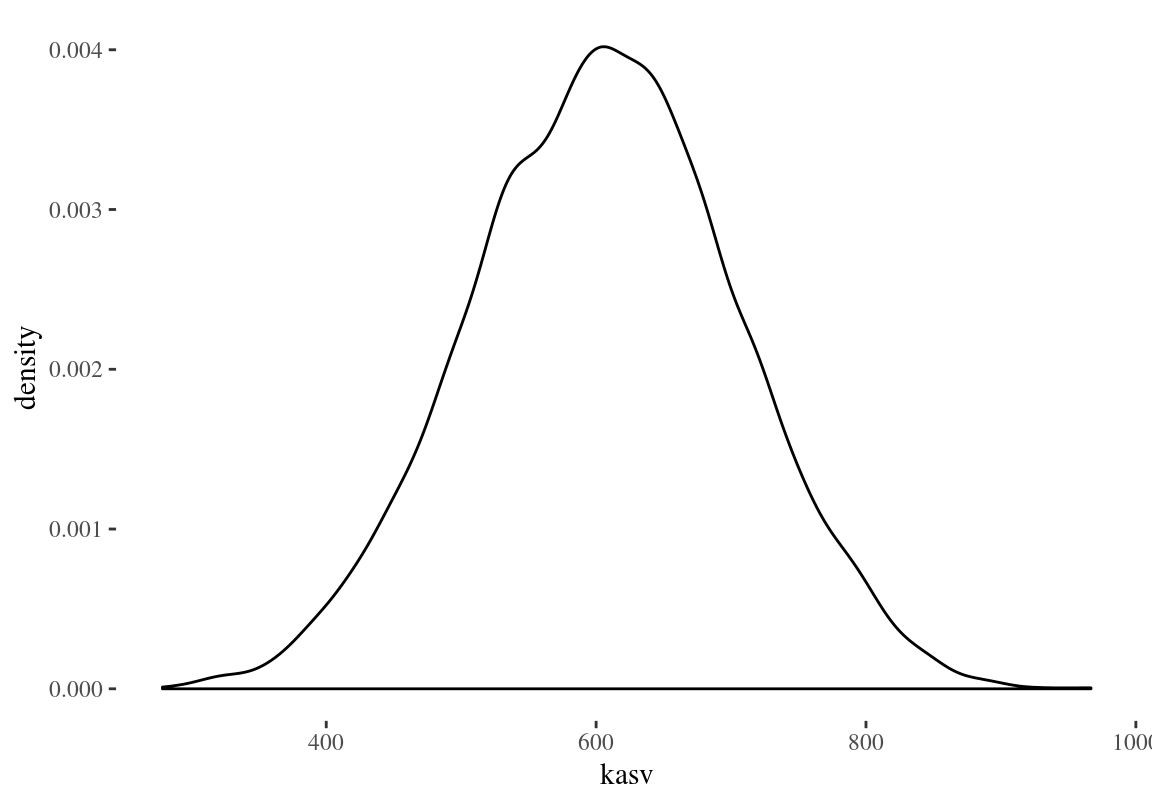
\includegraphics{06_veamudel_files/figure-latex/normaaljaotus-tekib-1.pdf}
\caption{\label{fig:normaaljaotus-tekib}Normaaljaotus tekib sõltumatutest efektidest.
Kümne tuhande N = 12 suuruse juhuvalimi summa tihedusdiagramm.}
\end{figure}

Selles näites võrdub iga andmepunkt 10 000st ühe bakteritüve
kasvukiiruse mõõtmisega. Seega, antud eelduste korral on bakteritüvede
kasvukiirused normaaljaotusega.

Nüüd vaatame, mis juhtub, kui 12 geeni mõjud ei ole üksteisest
sõltumatud. Kui 12 geeni on omavahel vastasmõjudes, siis nende geenide
mõjud korrutuvad, mitte ei liitu. (Korrutamine pole ainus viis, kuidas
vastasmõjusid modeleerida, küll aga kõige levinum.) Kõigepealt vaatleme
juhtu, kus 12 geeni on kõik väikeste mõjudega ning seega mitte ühegi
geeni mõju ei domineeri teiste üle. Seekord genreerime 12 juhuslikku
arvu 1 ja 1.1 vahel. Siin tähendab arv 1.1 kasvu tõusu 10\% võrra.
Seejärel korrutame need 12 arvu, misjärel kordame eelnevat 10 000 korda.





\begin{Shaded}
\begin{Highlighting}[]
\NormalTok{kasv <-}\StringTok{ }\KeywordTok{replicate}\NormalTok{(}\DecValTok{10000}\NormalTok{, }\KeywordTok{prod}\NormalTok{(}\KeywordTok{runif}\NormalTok{(}\DecValTok{12}\NormalTok{, }\DecValTok{1}\NormalTok{, }\FloatTok{1.1}\NormalTok{))) }
\NormalTok{p }\OperatorTok\StringTok{ }\KeywordTok{tibble}\NormalTok{(kasv)}
\end{Highlighting}
\end{Shaded}

\begin{figure}
\centering
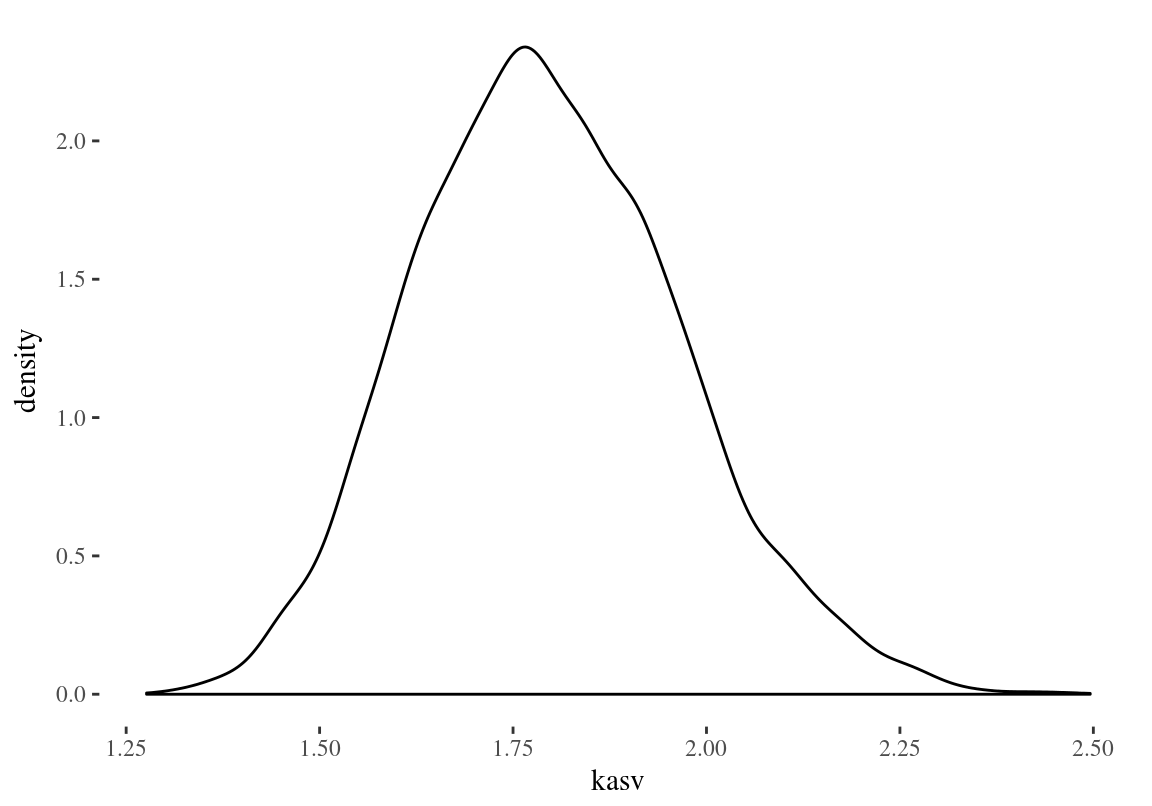
\includegraphics{06_veamudel_files/figure-latex/soltuvatest-efektidest-1.pdf}
\caption{\label{fig:soltuvatest-efektidest}Normaaljaotus tekib väikestest sõltuvatest
efektidest. Kümne tuhande N = 12 suuruse juhuvalimi korrutiste
tihedusdiagramm. Ühegi geeni mõju ei domineeri teiste üle.}
\end{figure}

Tulemuseks on jällegi normaaljaotus. Selles näites olid üksikud
interakteeruvad geenid ükshaaval väikeste mõjudega ja ühegi geeni mõju
ei domineerinud teiste üle. Mis juhtub, kui mõnel geenil on kuni 2 korda
suurem mõju kui teisel?





\begin{Shaded}
\begin{Highlighting}[]
\NormalTok{kasv <-}\StringTok{ }\KeywordTok{replicate}\NormalTok{(}\DecValTok{10000}\NormalTok{, }\KeywordTok{prod}\NormalTok{(}\KeywordTok{runif}\NormalTok{(}\DecValTok{12}\NormalTok{, }\DecValTok{1}\NormalTok{, }\DecValTok{2}\NormalTok{)))}
\NormalTok{p }\OperatorTok\StringTok{ }\KeywordTok{tibble}\NormalTok{(kasv)}
\end{Highlighting}
\end{Shaded}

\begin{figure}
\centering
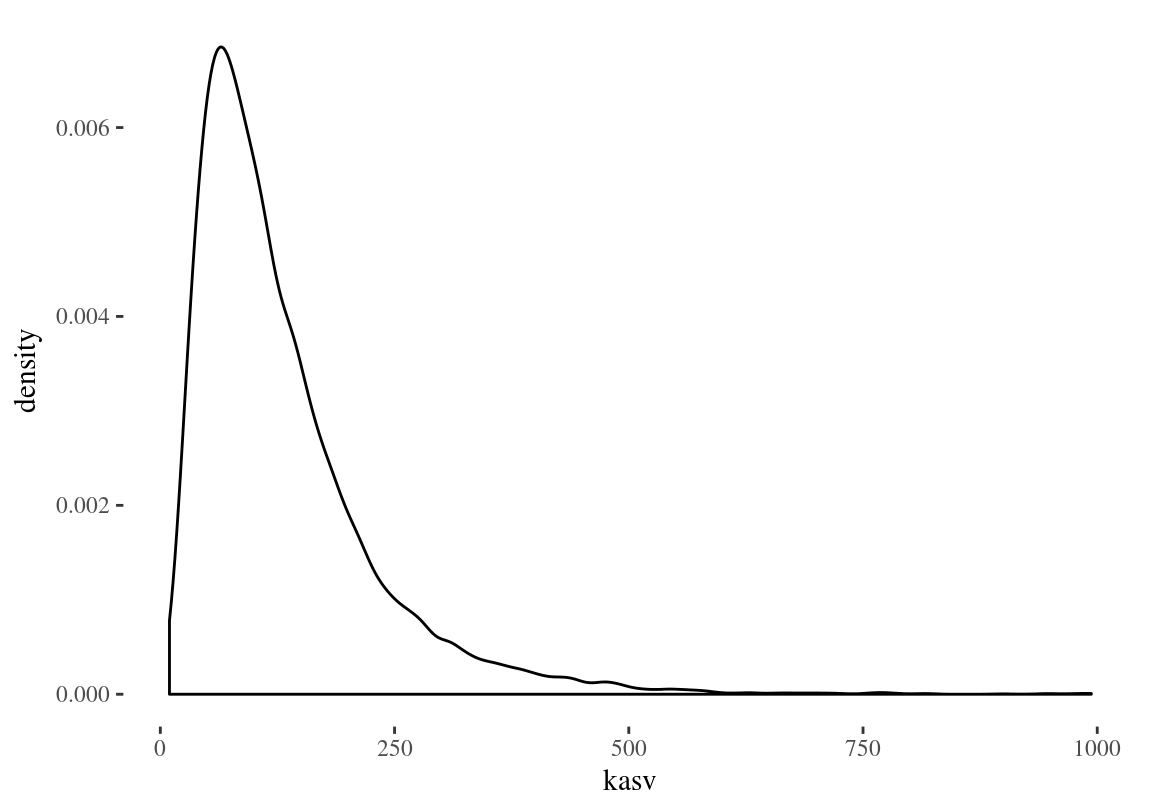
\includegraphics{06_veamudel_files/figure-latex/lognormaal-1.pdf}
\caption{\label{fig:lognormaal}Lognormaaljaotus tekib suurematest sõltuvatest
efektidest. Kümne tuhande N = 12 suuruse juhuvalimi korrutiste
tihedusdiagramm. Mõnel geenil on kuni 2 korda suurem mõju kui teisel.}
\end{figure}

Nüüd on tulemuseks log-normaaljaotus. Mis teie arvate, kas teie poolt
uuritavat tunnust mõjutavad faktorid, mis omavahel ei interakteeru või
kui interakteeruvad, on kõik ühtlaselt väikeste efektidega? Või on tegu
vastasmõjudes olevate faktoritega, millest osad on palju suuremate
mõjudega, kui teised? Ühel juhul eelistate te normaaljaotust, teisel
juhul peate õppima töötama ka lognormaaljaotusega.

Kui me vaatame samu andmeid logaritmilises skaalas, avastame, et need
andmed on normaaljaotusega. See ongi andmete logaritmimise mõte.





\begin{Shaded}
\begin{Highlighting}[]
\NormalTok{kasv <-}\StringTok{ }\KeywordTok{replicate}\NormalTok{(}\DecValTok{10000}\NormalTok{, }\KeywordTok{log10}\NormalTok{(}\KeywordTok{prod}\NormalTok{(}\KeywordTok{runif}\NormalTok{(}\DecValTok{12}\NormalTok{, }\DecValTok{1}\NormalTok{, }\DecValTok{2}\NormalTok{))))}
\NormalTok{p }\OperatorTok\StringTok{ }\KeywordTok{tibble}\NormalTok{(kasv) }\OperatorTok{+}\StringTok{ }\KeywordTok{labs}\NormalTok{(}\DataTypeTok{x =} \StringTok{"kasv, log10"}\NormalTok{)}
\end{Highlighting}
\end{Shaded}

\begin{figure}
\centering
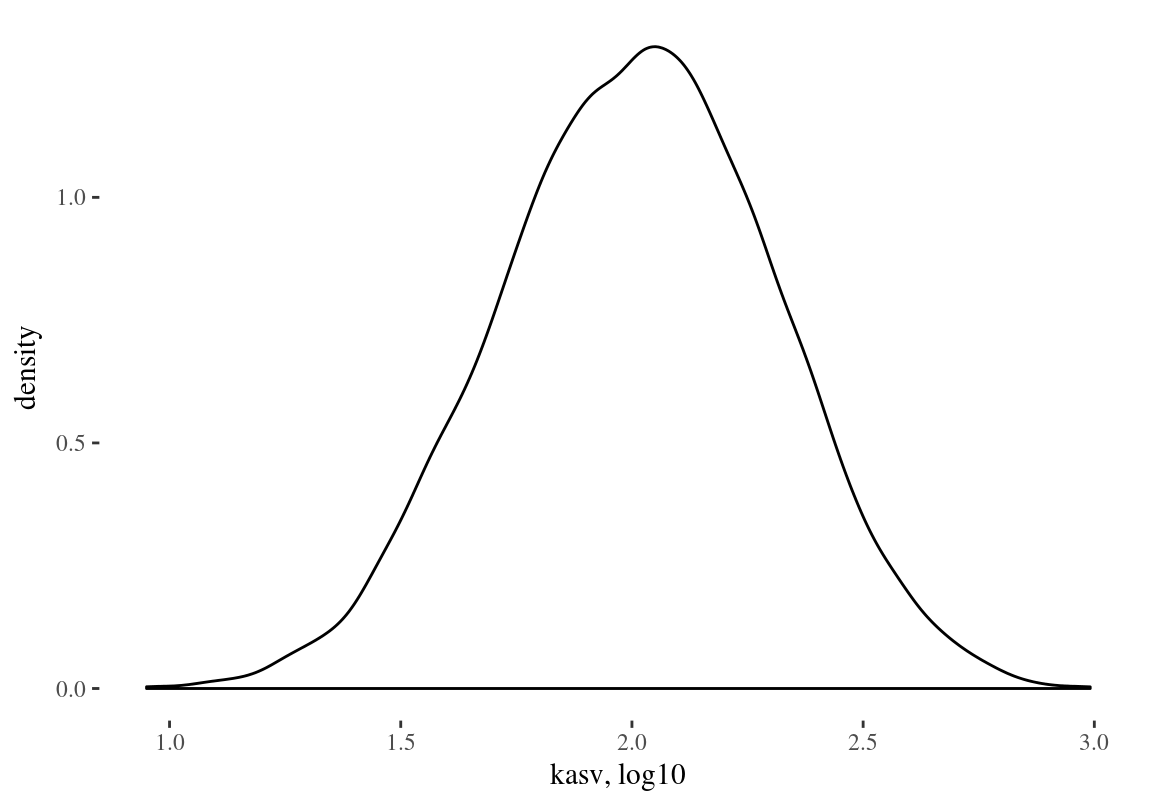
\includegraphics{06_veamudel_files/figure-latex/logskaalas-1.pdf}
\caption{\label{fig:logskaalas}Logaritmilises skaalas lognormaalsed efektid on
normaaljaotusega. Kümne tuhande N = 12 suuruse juhuvalimi korrutiste
tihedusdiagramm. Mõnel geenil on kuni 2 korda suurem mõju kui teisel.}
\end{figure}

\begin{quote}
Normaaljatuse avastas Gauss (1809), aga nime andis sellele Francis
Galton (1860ndatel), kuna antropoloogilised mõõtmised ``normaalselt''
järgisid ``vigade seadust'', mille ta nimetas ``Normaalseks jaotuste
kurviks''.
\end{quote}

\subsection*{Normaaljaotuse mudel väikestel
valimitel}\label{normaaljaotuse-mudel-vaikestel-valimitel}
\addcontentsline{toc}{subsection}{Normaaljaotuse mudel väikestel
valimitel}

Oletame, et meil on kolm andmepunkti ning me usume, et need andmed on
juhuslikult tõmmatud normaaljaotusest või sellele lähedasest jaotusest.
Normaaljaotuse mudelit kasutades deklareerime, et me usume, et kui
oleksime olnud vähem laisad ja 3 mõõtmise asemel sooritanuks 3000, siis
need mõõtmised sobituksid piisavalt hästi meie 3 väärtuse peal fititud
normaaljaotusega. Seega, me usume, et omades 3 andmepunkti me teame juba
umbkaudu, millised tulemused me oleksime saanud korjates näiteks 3
miljonit andmepunkti. Oma mudelist võime simuleerida ükskõik kui palju
andmepunkte.

Aga pidage meeles, et selle mudeli fittimiseks kasutame me ainult neid
andmeid, mis meil päriselt on --- ja kui meil on ainult 3 andmepunkti,
on tõenäoline, et fititud mudel ei kajasta hästi tegelikkust.

Kuidas panna skeptik uskuma, et statistilised meetodid töötavad halvasti
väikestel valimitel? Järgnevalt illustreerime seda ühe võimaliku
valimiga paljudest, mis on tõmmatud imaginaarsest populatsioonist, mille
parameetreid me teame. Me tõmbame 3-se valimi ning üritame selle valimi
põhjal ennustada selleasama populatsiooni struktuuri. Kuna tegemist on
simulatsiooniga, teame täpselt, et populatsioon, kust me tõmbame oma
kolmese valimi, on normaaljaotusega, et tema keskväärtus = 0 ja et tema
sd = 1. Seega saame võrrelda oma ennustust populatsiooni tõeliste
parameetriväärtustega. Me fitime oma valimiandmetega 2 erinevat mudelit:
normaaljaotuse ja Studenti t jaotuse.









\begin{figure}
\centering
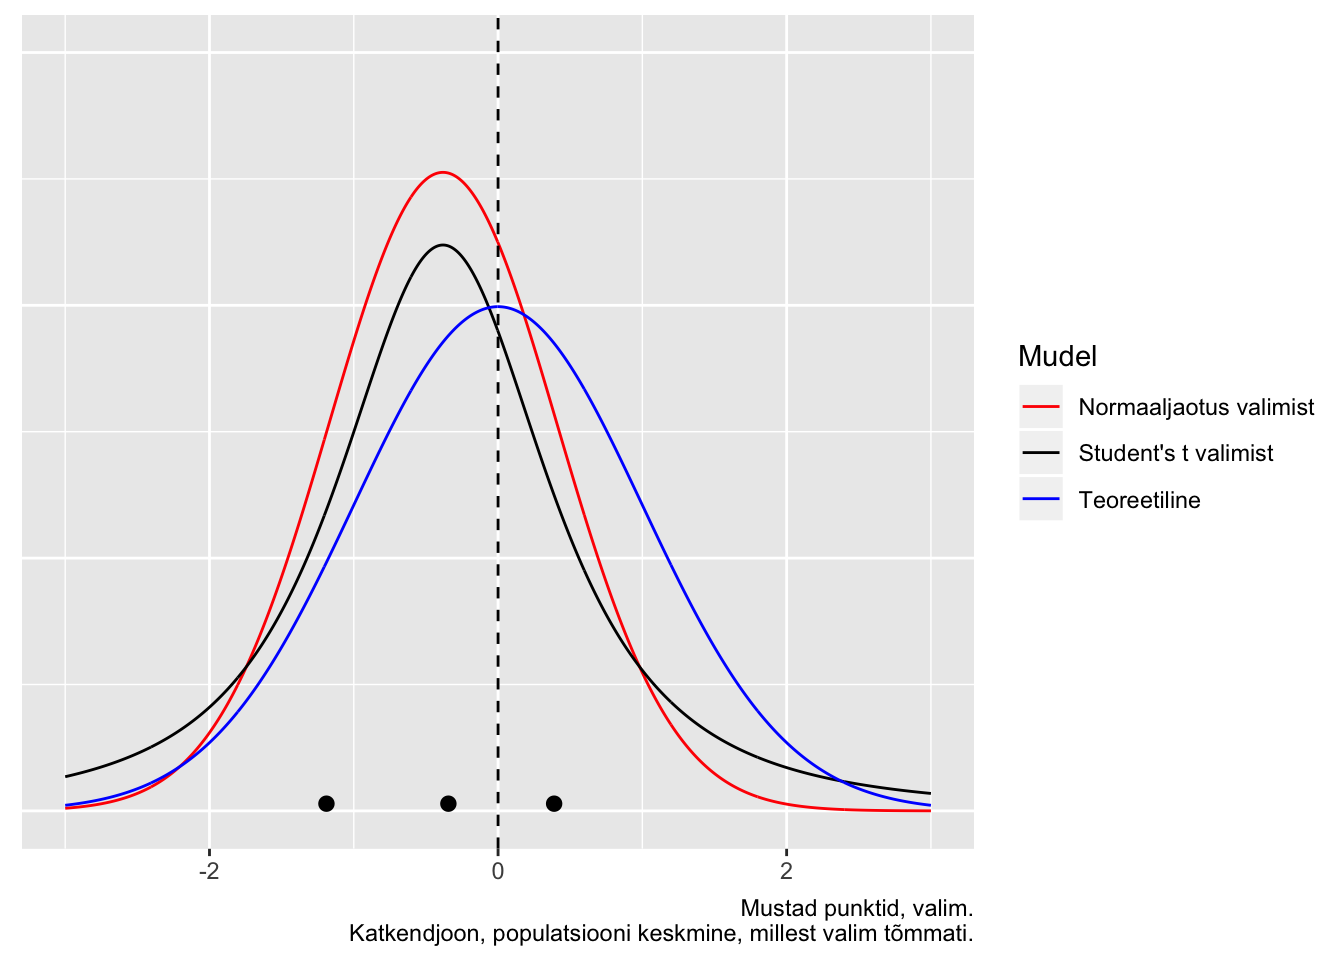
\includegraphics{06_veamudel_files/figure-latex/juhuvalim-normaaljaotusest-1.pdf}
\caption{\label{fig:juhuvalim-normaaljaotusest}Juhuvalim normaaljaotusest, mille
keskmine = 0 ja sd = 1 (n=3; andmepunktid on näidatud mustade munadena).
Sinine joon - populatsioon, millest tõmmati valim; punane joon -
normaaljaotuse mudel, mis on fititud valimi andmetel; must joon -
Studenti t jaotuse mudel, mis on fititud samade andmetega. Mustad
punktid, valim. Katkendjoon, populatsiooni keskmine, millest valim
tõmmati.}
\end{figure}

Siin saame hinnata mudelite fitte jumala positsioonilt, võrreldes
fititud mudelite jaotusi ``tõese'' sinise jaotusega. Mõlemad mudelid on
süstemaatiliselt nihutatud väiksemate väärtuste poole ja alahindavad
varieeruvust. t jaotuse mudel on oodatult paksemate sabadega ja ennustab
0-st kaugele palju rohkem väärtusi kui normaaljaotuse mudel. Kuna me
teame, et populatsioon on normaaljaotusega, pole väga üllatav, et t
jaotus modeleerib seda halvemini kui normaaljaotus.

Igal juhul, mõni teine juhuvalim annaks meile hoopis teistsugused
mudelid, mis rohkem või vähem erinevad algsest populatsioonist.

Mis juhtub kui me kasutame oma normaaljaotuse mudelit uute andmete
simuleerimiseks? Kui lähedased on need simuleeritud andmed populatsiooni
andmetega ja kui lähedased valimi andmetega, millega me normaaljaotuse
mudeli fittisime?




\begin{Shaded}
\begin{Highlighting}[]
\CommentTok{# tõmbame 3 juhuslikku arvu normaalhaotusest, mille keskväärtus = 0 ja sd = 1.}
\NormalTok{dfr <-}\StringTok{ }\KeywordTok{tibble}\NormalTok{(}\DataTypeTok{sample_data =} \KeywordTok{rnorm}\NormalTok{(}\DecValTok{3}\NormalTok{)) }
\NormalTok{dfr <-}\StringTok{ }\KeywordTok{summarise_at}\NormalTok{(dfr, }\StringTok{"sample_data"}\NormalTok{, }\KeywordTok{c}\NormalTok{(}\StringTok{"mean"}\NormalTok{, }\StringTok{"sd"}\NormalTok{))}
\NormalTok{dfr}
\CommentTok{#> # A tibble: 1 x 2}
\CommentTok{#>     mean    sd}
\CommentTok{#>    <dbl> <dbl>}
\CommentTok{#> 1 0.0654 0.808}
\CommentTok{# simuleerime 1000 uut andmepunkti fititud mudelist}
\NormalTok{simulated_data <-}\StringTok{ }\KeywordTok{rnorm}\NormalTok{(}\DecValTok{1000}\NormalTok{, dfr}\OperatorTok{$}\NormalTok{mean, dfr}\OperatorTok{$}\NormalTok{sd)}
\CommentTok{# arvutame simuleeritud andmete keskmise ja sd ning joonistame neist histogrammi}
\KeywordTok{ggplot}\NormalTok{(}\KeywordTok{tibble}\NormalTok{(simulated_data), }\KeywordTok{aes}\NormalTok{(simulated_data)) }\OperatorTok{+}
\StringTok{  }\KeywordTok{geom_histogram}\NormalTok{(}\DataTypeTok{bins =} \DecValTok{15}\NormalTok{)}
\end{Highlighting}
\end{Shaded}

\begin{figure}
\centering
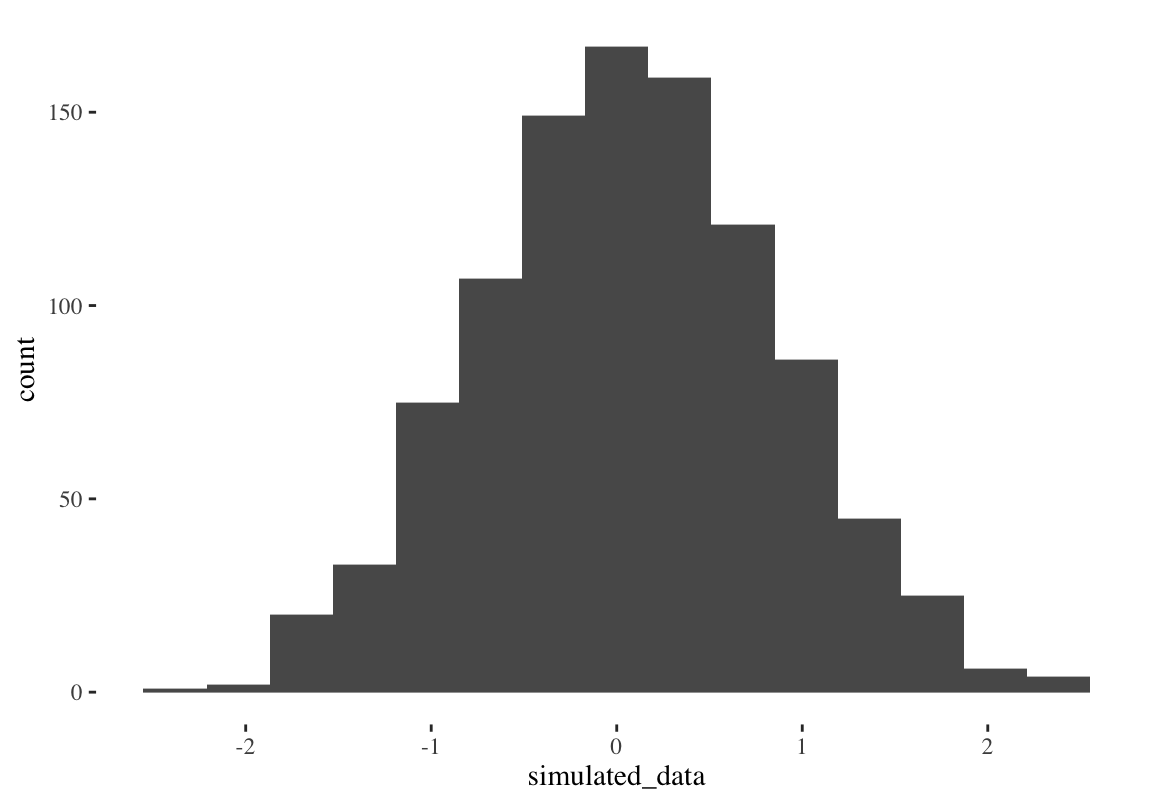
\includegraphics{06_veamudel_files/figure-latex/kasutame-fititud-1.pdf}
\caption{\label{fig:kasutame-fititud}Kasutame fititud mudeleid uute andmete
simuleerimiseks.}
\end{figure}

Nagu näha, igati ootuspäraselt on uute (simuleeritud) andmete
keskväärtus ja SD väga sarnased algsete andmete omale, mida kasutasime
mudeli fittimisel. Kahjuks ei ole need aga kaugeltki nii sarnased
algsele jaotusele, mille kuju me püüame oma andmete ja mudeli pealt
ennustada. Seega on meie mudel üle-fittitud, mis tähendab, et ta
kajastab liigselt neid valimi aspekte, mis ei peegelda algse
populatsiooni omadusi. Loomulikult ei vasta ükski mudel päriselt
tegelikkusele. Küsimus on pigem selles, kas mõni meie mudelitest on
piisavalt hea, et olla kasulik. Vastus sellele sõltub, milleks plaanime
oma mudelit kasutada.

\begin{Shaded}
\begin{Highlighting}[]
\KeywordTok{mean}\NormalTok{(simulated_data }\OperatorTok{>}\StringTok{ }\DecValTok{0}\NormalTok{) }
\CommentTok{#> [1] 0.535}
\KeywordTok{mean}\NormalTok{(simulated_data }\OperatorTok{>}\StringTok{ }\DecValTok{1}\NormalTok{)}
\CommentTok{#> [1] 0.116}
\end{Highlighting}
\end{Shaded}

Kui populatsiooniväärtustest on 50\% suuremad kui 0, siis mudeli järgi
vaevalt 32\%. Kui populatsiooniväärtustest on 16\% suuremad kui 1, siis
mudeli järgi vaevalt 4\%. See illustreerib hästi mudeli kvaliteeti.

\begin{Shaded}
\begin{Highlighting}[]
\NormalTok{sim_t <-}\StringTok{ }\KeywordTok{rstudent_t}\NormalTok{(}\DecValTok{1000}\NormalTok{, }\DecValTok{2}\NormalTok{, dfr}\OperatorTok{$}\NormalTok{mean, dfr}\OperatorTok{$}\NormalTok{sd)}
\KeywordTok{mean}\NormalTok{(sim_t }\OperatorTok{>}\StringTok{ }\DecValTok{0}\NormalTok{)}
\CommentTok{#> [1] 0.516}
\KeywordTok{mean}\NormalTok{(sim_t }\OperatorTok{>}\StringTok{ }\DecValTok{1}\NormalTok{)}
\CommentTok{#> [1] 0.189}
\end{Highlighting}
\end{Shaded}

Samad ennustused t jaotusest on isegi paremad! Aga kumb on ikkagi parem
mudel populatsioonile?

\section*{Normaaljaotuse ja lognormaaljaotuse
erilisus}\label{normaaljaotuse-ja-lognormaaljaotuse-erilisus}
\addcontentsline{toc}{section}{Normaaljaotuse ja lognormaaljaotuse
erilisus}

Normaaljaotus ja lognormaaljaotus on erilised sest

\begin{enumerate}
\def\labelenumi{(\arabic{enumi})}
\tightlist
\item
  kesksest piirteoreemist (\emph{central limit theorem}) tuleneb, et
  olgu teie valim ükskõik millise jaotusega, paljudest valimitest
  arvutatud \textbf{aritmeetilised keskmised} on alati enam-vähem
  normaaljaotusega. See kehtib enamuse andmejaotuste korral, kui
  n\textgreater{}30. Selle matemaatilise tõe peegeldus füüsikalisse
  maailma on ``elementaarsete vigade hüpotees'', mille kohaselt paljude
  väikeste üksteisest sõltumatute juhuslike efektide (vigade) summa
  annab tulemuseks normaaljaotuse.
\end{enumerate}

Paraku enamus bioloogilisi mõõtmisi annavad tulemuseks eranditult
mitte-negatiivseid väärtusi. Sageli on selliste väärtuste jaotused
ebasümmeetrilised (v.a. siis, kui cv = sd/mean on väike), ja kui nii,
siis on meil sageli tegu lognormaaljaotusega, mis tekkib log-normaalsete
muutujate korrutamisest. Siit tuleb Keskne piirteoreem 2, mille kohaselt
suvalise jaotusega muutujate \textbf{geomeetrilised keskmised} on
enam-vähem lognormaaljaotusega, ning elementaarsete vigade hüpotees 2:
Kui juhuslik varieeruvus tekib paljude juhuslike efektide korrutamisel,
on tulemuseks lognormaaljaotus. Lognormaaljaotusega väärtuste
logaritmimine annab normaaljaotuse.

\begin{enumerate}
\def\labelenumi{(\arabic{enumi})}
\setcounter{enumi}{1}
\tightlist
\item
  Nii normaal- kui lognormaaljaotus on maksimaalse entroopiaga jaotused.
  Entroopiat vaadeldakse siin informatsiooni \& müra kaudu ---
  maksimaalse entroopiaga süsteem sisaldab maksimaalselt müra ja
  minimaalselt informatsiooni (vastavalt Shannoni
  informatsiooniteooriale). See tähendab, et väljaspool oma parameetrite
  tuunitud väärtusi on normaal- ja lognormaaljaotused minimaalselt
  informatiivsed. Normaaljaotusel ja lognormaaljaotusel on kummagil kaks
  parameetrit, \emph{mu} ja \emph{sigma} (ehk keskmine ja
  standardhälve), mille väärtused fikseerides fikseerime üheselt jaotuse
  ehk mudeli kuju, lisades sinna minimaalselt muud (sooviamtut)
  informatsiooni. Teised maksimaalse entroopiaga jaotused on näiteks
  eksponentsiaalne jaotus, binoomjaotus, bernoulli jaotus, poissoni
  jaotus.
\end{enumerate}

\begin{quote}
Kui meil on tegu nullist suuremate andmetega, on andmete logaritmimine
sageli hea mõte. Logaritmitud andmete pealt arvutatud keskmise ja sd
eksponentimine annab meile geomeetrilise keskmise (exp(mu) = mu\_geom)
ja multiplikatiivse sd (exp(sd) = sd\_mult).
\end{quote}

Kui me fitime lognormaaljaotust andmetega, siis fititud koefitsiendid mu
ja sd tuleb eksponentida, et saada geomeetriline keskmine ja
multiplikatiivne sd.

mu\_geom x sd\_mult \ldots{} mu\_geom/sd\_mult annab vahemiku, kuhu jääb
68\% lognormaalsetest andmetest ja mu\_geom x 2sd\_mult \ldots{}
mu\_geom/2sd\_mult annab vahemiku, kuhu jääb 96\% andmetest (just nagu
additiivne sd tõõtab aritmeetilise additiivse keskmisega normaalsete
andmete korral).

Maksimaalsel entroopial põhineb normaaljaotuse ja lognormaaljaotuse sage
kasutamine Bayesi statistikas prioritena, sest me suudame paremini
kontrollida, millist informatsiooni me neisse surume. Esimesel kesksel
piirteoreemil seevastu põhineb kogu sageduslik statistika (vt ptk 8.).

\subsection{Normaaljaotuse ja lognormaaljaotuse
võrdlus}\label{normaaljaotuse-ja-lognormaaljaotuse-vordlus}

\textbf{Normaaljaotus}

\begin{enumerate}
\def\labelenumi{\arabic{enumi}.}
\item
  Normaaljaotusega ehk normaalsete juhuslike muutujate liitmine annab
  normaalse summa. Lineaarsed kombinatsioonid
  \(Y= \alpha + \beta_1X_1 + \beta_2X_2\) jäävad normaalseks.
\item
  Normaalsete muutujate aritmeetilised keskmised on normaaljaotusega.
\item
  Keskne piirteoreem: mitte-normaalsete muutujate aritmeetilised
  keskmised on enam-vähem normaaljaotusega.
\item
  Elementaarsete vigade hüpotees: kui juhuslik varieeruvus on paljude
  juhuslike mõjude summa, on tulemuseks normaaljaotus.
\item
  Additiivne regressioonimudel (normaalne tõepära) viib additiivsetele
  vigadele (residuaalidele), mis omakorda viib konstantsele
  varieeruvusele (SD-le). Vead on normaaljaotusega.
\end{enumerate}

\textbf{lognormaaljaotus}

\begin{enumerate}
\def\labelenumi{\arabic{enumi}.}
\item
  lognormaalsete juhuslike muutujate korrutamine annab lognormaalse
  korrutise.
\item
  Longnormaalsete muutujate geomeetrilised keskmised on
  lognormaaljaotusega.
\item
  Keskne piirteoreem: mitte-lognormaalsete muutujate geomeetrilised
  keskmised on enam-vähem lognormaaljaotusega
\item
  Elementaarsete vigade hüpotees: kui juhuslik varieeruvus on paljude
  juhuslike mõjude korrutis, on tulemuseks lognormaaljaotus
\item
  multiplikatiivne regressioonimudel (lognormaalne tõepära) viib
  multiplikatiivsete vigadeni ja konstantsele suhtelisele varieeruvusele
  (CV-le). Vigade jaotus on ebasümmeetriline.
\end{enumerate}

Seega võime lognormaaljaotust kutsuda ka multiplikatiivseks
normaaljaotuseks.

\section{Teised veamudelid}\label{teised-veamudelid}

\subsection{Lognormaaljaotus}\label{lognormaaljaotus}

\begin{Shaded}
\begin{Highlighting}[]
\NormalTok{x <-}\StringTok{ }\KeywordTok{seq}\NormalTok{(}\DecValTok{0}\NormalTok{, }\DecValTok{10}\NormalTok{, }\DataTypeTok{length.out =} \DecValTok{1000}\NormalTok{)}
\NormalTok{y <-}\StringTok{ }\KeywordTok{dlnorm}\NormalTok{(x)}
\KeywordTok{plot}\NormalTok{(x, y, }\DataTypeTok{typ =} \StringTok{"l"}\NormalTok{)}
\end{Highlighting}
\end{Shaded}

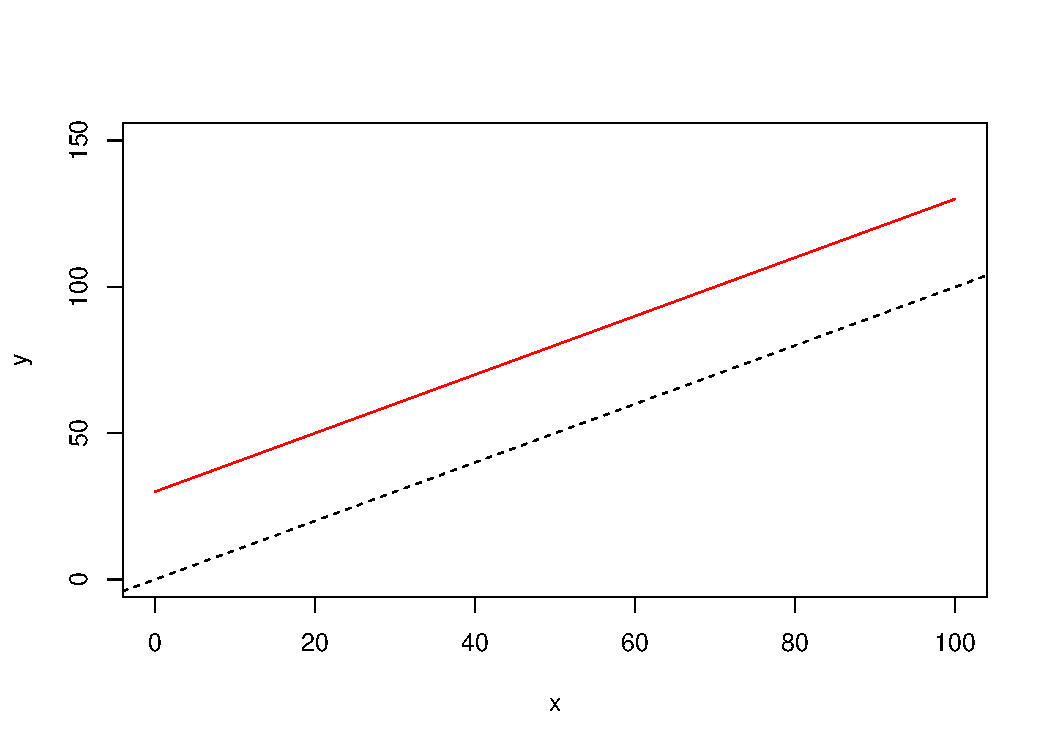
\includegraphics{06_veamudel_files/figure-latex/unnamed-chunk-10-1.pdf}

Seda jaotust, mis ei ulatu kunagi teisele poole nulli, iseloomustab, et
x-i logaritmimine annab tulemuseks normaaljaotuse.

\begin{Shaded}
\begin{Highlighting}[]
\KeywordTok{plot}\NormalTok{(}\KeywordTok{log}\NormalTok{(x), y, }\DataTypeTok{type =} \StringTok{"l"}\NormalTok{)}
\end{Highlighting}
\end{Shaded}

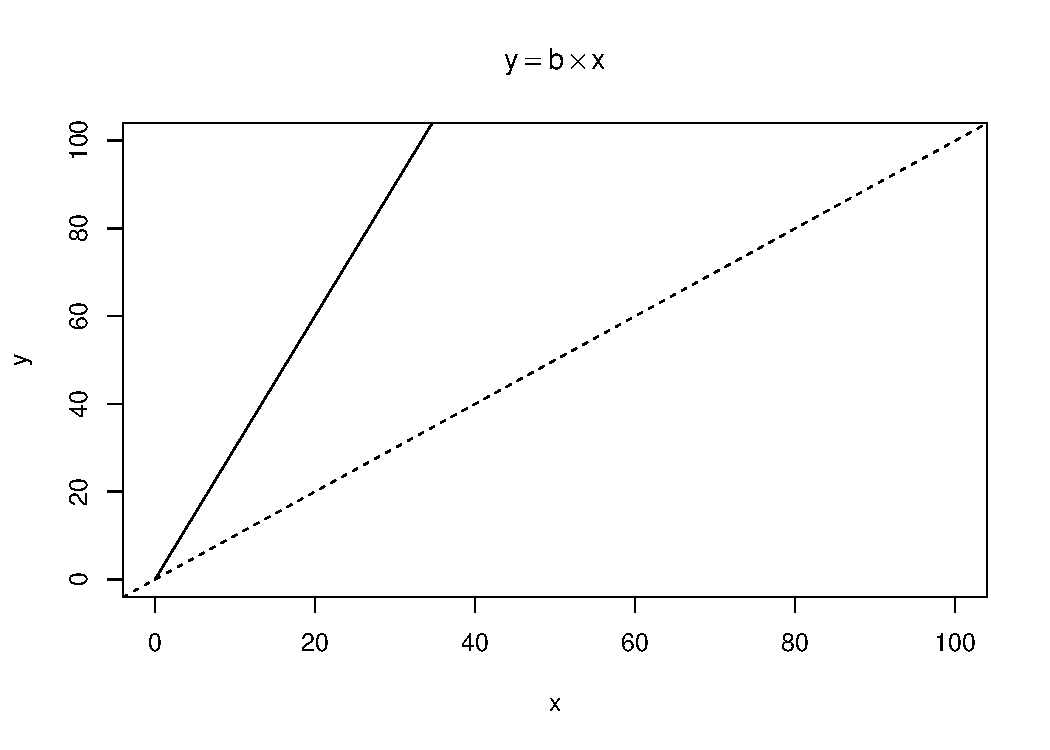
\includegraphics{06_veamudel_files/figure-latex/unnamed-chunk-11-1.pdf}

Lognormaaljaotuse keskväärtus, standardhälve, mood ja mediaan:

\[keskv\ddot{a}\ddot{a}rtus = \exp(\mu + 1/2 \times \sigma^2)\]

\[sd = \exp(\mu + 1/2 \times \sigma^2) \times \sqrt{\exp(\sigma^2) - 1}\]
\[mood = e^{\mu - \sigma^2}\]

\[mediaan = e^\mu\] Siin on siis \(\mu\) ja \(\sigma\) arvutatud
logaritmitud andmete pealt.

\subsection{Binoomjaotus}\label{binoomjaotus}

Kui teil on binaarne muutuja (sellel saab olla ainult kaks väärtust,
näiteks sees/väljas, 1/0), mis kajastab sõltumatuid sündmusi, siis
modelleerib seda binoomjaotus \(y \sim Binomial(n, p)\). Kus \emph{n} on
edukate sündmuste arv ja \emph{p} on nende suhteline sagedus (p = n / N,
kus \emph{N} on kõikide sündmuste kopguarv). Sõltumatud sündmused on
sellised, kus ühe sündmuse esinemise järgi ei saa ennustada teise
sündmuse esinemist (st puudub korrelatsioon sündmuste esinemise vahel).
Tehniliselt on binoomjaotusel veel omadus, et valim võetakse
replacementiga, mis tähendab, et iga sündmus pannakse populatsiooni
tagasi, kus seda saab uuesti valimisse tõmmata. Siit tuleb, et
binoomjaotuse mudel kehtib päris maailmas mõõndustega ja et seda mudelit
on kindlam kasutada siis, kui N \textgreater{}\textgreater{} n. Kui N on
suur, siis meenutab binoomjaotus normaaljaotust (läheneb selle kujule).

\begin{Shaded}
\begin{Highlighting}[]
\NormalTok{n <-}\StringTok{ }\DecValTok{10} \CommentTok{# sündmuste koguarv}
\NormalTok{x <-}\StringTok{ }\KeywordTok{seq}\NormalTok{(}\DecValTok{0}\NormalTok{, n) }\CommentTok{# kõik võimalikud õnnestumiste arvud 10st sündmusest}
\NormalTok{p <-}\StringTok{ }\FloatTok{0.3} \CommentTok{# 30% õnnestumisi (sagedus)}
\NormalTok{y <-}\StringTok{ }\KeywordTok{dbinom}\NormalTok{(x, n, p)}
\KeywordTok{plot}\NormalTok{(x, y)}
\end{Highlighting}
\end{Shaded}

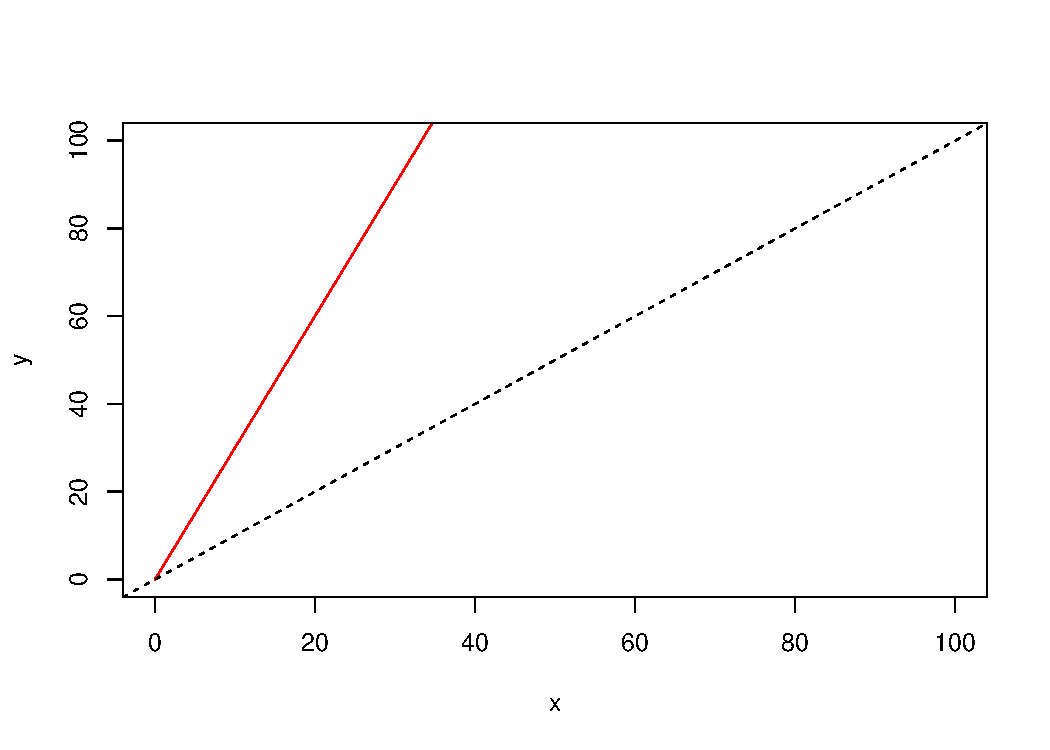
\includegraphics{06_veamudel_files/figure-latex/unnamed-chunk-12-1.pdf}

\[keskv\ddot{a}\ddot{a}rtus = N \times p\]

Kui Np võrdub täisarvuga, siis mediaan = mood = keskväärtus

\[sd = sqrt(N \times p(1 - p))\]

Standardviga proportsioonile \(p = \sqrt{\frac{p(1 - p)}{N}}\) See
standardviga (\emph{standard error}) on teiste sõnadega standardhälve
meie hinangule proportsiooni väärtusele. Kui n = 0 või N - n = 0, siis
on selline SE arvutus eksitav.

\subsection{Poissoni jaotus}\label{poissoni-jaotus}

See jaotus modelleerib üksikuid haruldasi ja sõltumatuid diskreetseid
sündmusi, mille arvu me saame üles lugeda. Näiteks surmi ajaühiku kohta
või pommitabamusi pindalaühiku kohta. Poissoni jaotus on binoomjaotuse
erijuht. Lisaeeldused on, et sündmuste toimumise sagedus ei muutu, et
kaks sündmust ei saa toimuda täpselt samal ajal/kohas, et sündmuse
toimumise tõenäosus on proportsionaalne intervalli pikkusega/suurusega
(ajas või ruumis) ja et N \textgreater{}\textgreater{} n.

Kui keskmine sündmuste arv intevallis on \(\lambda\) (lambda), siis

\[P(k~events~in~interval) = e^{\lambda} \times \frac{\lambda ^{k}}{k!}\]

Oodatud väärtus = variance = \(\lambda\)

\(sd = \sqrt{\lambda}\)

Millal kasutada Poissoni jaotust, ja millal binoomjaotust? Kui iga
andmepunkti saab vaadelda kui edukate katsete arvu suhet kõikide katsete
arvule, siis kasuta binoomjaotust/logistilist regressiooni. Kui aga
andmepunkti väärtusel pole loomulikku piiri (see on lihtsalt mingit
tüüpi sündmuste arv), kasuta Poissoni/logaritmilist regressiooni.

\chapter{EDA --- eksploratoorne
andmeanalüüs}\label{eda-eksploratoorne-andmeanaluus}

\begin{Shaded}
\begin{Highlighting}[]
\KeywordTok{library}\NormalTok{(tidyverse)}
\KeywordTok{library}\NormalTok{(corrgram)}
\KeywordTok{library}\NormalTok{(psych)}
\KeywordTok{library}\NormalTok{(skimr)}
\end{Highlighting}
\end{Shaded}

Kui ühenumbriline andmete summeerimine täidab eelkõige kokkuvõtliku
kommunikatsiooni eesmärki, siis EDA on suunatud teadlasele endale. EDA
eesmärk on andmeid eelkõige graafiliselt vaadata, et saada aimu 1)
andmete kvaliteedist ja 2) lasta andmetel kõneleda ``sellisena nagu nad
on'' ja sugereerida uudseid teaduslikke hüpoteese. Neid hüpoteese peaks
siis testima formaalse statistilise analüüsi abil (ptk järeldav
statistika). Näiteid erinevate graafiliste lahenduste kohta vt graafika
peatükist.

\begin{quote}
EDA: mida rohkem graafikuid, seda rohkem võimalusi uute mõtete tekkeks!
\end{quote}

EDA on rohkem kunst kui teadus selles mõttes, et teil on suur vabadus
küsida selle abil erinevaid küsimusi oma andmete kohta. Ja seda nii
tehnilisest aspektist lähtuvalt (milline on minu andmete kvaliteet?),
kui teaduslikke küsimusi küsides (kas muutuja A võiks põhjustada muutusi
muutujas B?).

Mõned üldised soovitused võib siiski anda.

\begin{enumerate}
\def\labelenumi{\arabic{enumi}.}
\tightlist
\item
  alusta analüüsi tasemest, kus andmed on kõige inforikkamad ---
  toorandmete plottimisest punktidena. Kui andmehulk ei ole väga
  massiivne, näitab see hästi nii andmete kvaliteeti, kui ka võimalikke
  sõltuvussuhteid erinevate muutujate vahel.
\end{enumerate}

Millised korrelatsioonid võiksid andmetes esineda?



\begin{Shaded}
\begin{Highlighting}[]
\KeywordTok{corrgram}\NormalTok{(iris, }
         \DataTypeTok{order =} \OtherTok{TRUE}\NormalTok{, }
         \DataTypeTok{lower.panel =}\NormalTok{ panel.pts,}
         \DataTypeTok{upper.panel =}\NormalTok{ panel.ellipse,}
         \DataTypeTok{diag.panel =}\NormalTok{ panel.density,}
         \DataTypeTok{main =} \StringTok{"Correlogram of Iris dataset"}\NormalTok{)}
\end{Highlighting}
\end{Shaded}

\begin{figure}
\centering
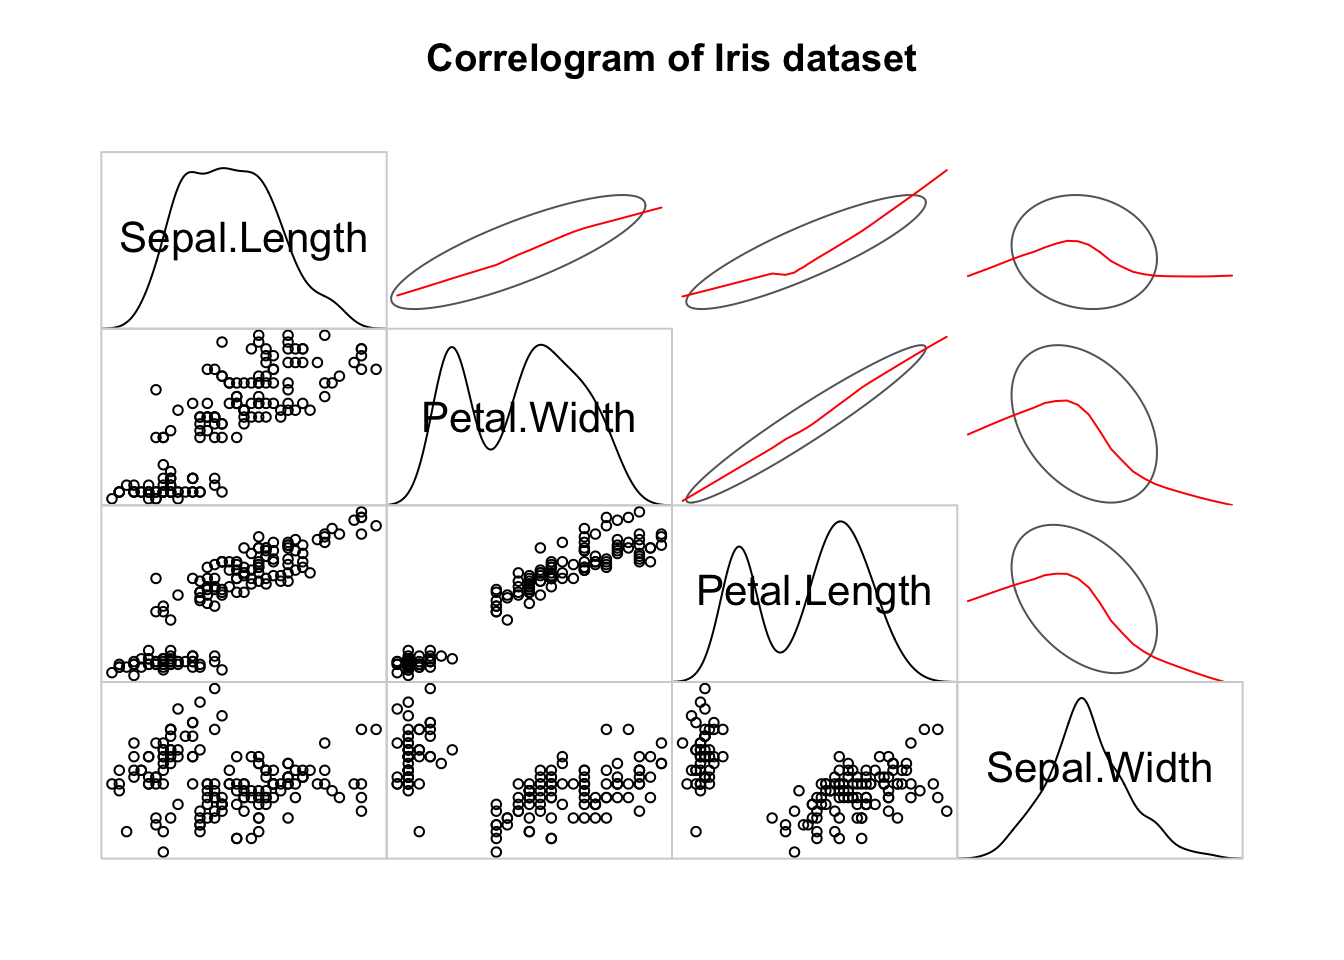
\includegraphics{07_EDA_files/figure-latex/korrmaatriks-1.pdf}
\caption{\label{fig:korrmaatriks}Korrelatstioonimaatriks joonisena.}
\end{figure}

\begin{enumerate}
\def\labelenumi{\arabic{enumi}.}
\setcounter{enumi}{1}
\tightlist
\item
  vaata andmeid numbrilise kokkuvõttena.
\end{enumerate}

\begin{Shaded}
\begin{Highlighting}[]
\NormalTok{psych}\OperatorTok{::}\KeywordTok{describe}\NormalTok{(iris) }
\CommentTok{#>              vars   n mean   sd median trimmed  mad min max range  skew}
\CommentTok{#> Sepal.Length    1 150 5.84 0.83   5.80    5.81 1.04 4.3 7.9   3.6  0.31}
\CommentTok{#> Sepal.Width     2 150 3.06 0.44   3.00    3.04 0.44 2.0 4.4   2.4  0.31}
\CommentTok{#> Petal.Length    3 150 3.76 1.77   4.35    3.76 1.85 1.0 6.9   5.9 -0.27}
\CommentTok{#> Petal.Width     4 150 1.20 0.76   1.30    1.18 1.04 0.1 2.5   2.4 -0.10}
\CommentTok{#> Species*        5 150 2.00 0.82   2.00    2.00 1.48 1.0 3.0   2.0  0.00}
\CommentTok{#>              kurtosis   se}
\CommentTok{#> Sepal.Length    -0.61 0.07}
\CommentTok{#> Sepal.Width      0.14 0.04}
\CommentTok{#> Petal.Length    -1.42 0.14}
\CommentTok{#> Petal.Width     -1.36 0.06}
\CommentTok{#> Species*        -1.52 0.07}
\end{Highlighting}
\end{Shaded}

\begin{Shaded}
\begin{Highlighting}[]
\NormalTok{skimr}\OperatorTok{::}\KeywordTok{skim}\NormalTok{(iris) }
\CommentTok{#> Skim summary statistics}
\CommentTok{#>  n obs: 150 }
\CommentTok{#>  n variables: 5 }
\CommentTok{#> }
\CommentTok{#> -- Variable type:factor ---------------------------------------}
\CommentTok{#>  variable missing complete   n n_unique                       top_counts}
\CommentTok{#>   Species       0      150 150        3 set: 50, ver: 50, vir: 50, NA: 0}
\CommentTok{#>  ordered}
\CommentTok{#>    FALSE}
\CommentTok{#> }
\CommentTok{#> -- Variable type:numeric --------------------------------------}
\CommentTok{#>      variable missing complete   n mean   sd  p0 p25  p50 p75 p100}
\CommentTok{#>  Petal.Length       0      150 150 3.76 1.77 1   1.6 4.35 5.1  6.9}
\CommentTok{#>   Petal.Width       0      150 150 1.2  0.76 0.1 0.3 1.3  1.8  2.5}
\CommentTok{#>  Sepal.Length       0      150 150 5.84 0.83 4.3 5.1 5.8  6.4  7.9}
\CommentTok{#>   Sepal.Width       0      150 150 3.06 0.44 2   2.8 3    3.3  4.4}
\end{Highlighting}
\end{Shaded}

Siin pööra kindlasti tähelepanu tulpadele min ja max, mis annavad kiire
võimalusi outliereid ära tunda. Kontrolli, kas andmete keskmised
(mediaan, mean ja trimmed mean) on üksteisele piisavalt lähedal --- kui
ei ole, siis on andmete jaotus pika õlaga, ja kindlasti mitte normaalne.
Kontrolli, kas erinevate muutujate keskväärtused ja hälbed on
teaduslikus mõttes usutavas vahemikus. Ära unusta, et ka väga väike
standardhälve võib tähendada, et teie valim ei peegelda bioloogilist
varieeruvust populatsioonis, mis teile teaduslikku huvi pakub. NB!
selles \texttt{psych::describe()} funktsiooni väljundis on mad läbi
korrutatud konstandiga \texttt{1.4826}, mis toob selle väärtuse lähemale
sd-le. Seega on mad siin sd robustne analoog --- kui mad on palju
väiksem sd-st, siis on karta, et muutujas on outliereid.

\begin{enumerate}
\def\labelenumi{\arabic{enumi}.}
\setcounter{enumi}{2}
\item
  kontrolli NA-de esinemist oma andmetes VIM paketi abil või käsitsi (vt
  esimene ptk). Kontrolli, et NA-d ei oleks tähistatud mingil muul
  viisil (näiteks 0-i või mõne muu numbriga). Kui vaja, rekodeeri NAd.
  Mõtle selle peale, millised protsessid looduses võiksid genreerida
  puuduvaid andmeid. Kui NA-d ei jaotu andmetes juhuslikult, võib olla
  hea mõte andmeid imputeerida (vt hilisemaid ptk, bayesiaanlik
  imputeerimine). Näiteks, kui ravimiuuringust kukuvad eeskätt välja
  patsiendid, kellel ravim ei tööta, on ilmselt halb mõte nende
  patsientide andmed lihtsalt uuringust välja vistata (muidugi, kui te
  ei esinda kasumit taotleva ettevõtte huve). Kui NA-d jaotuvad
  juhuslikult, mõtle sellele, kas sa tahad NA-dega read tabelist välja
  visata, või hoopis osad muutujad, mis sisaldavad liiga palju NA-sid,
  või mitte midagi välja vistata. NB! NA-dega andmed ei sobi hästi
  regresiooniks.
\item
  Kui andmeid on nii palju, et üksikute andmepunktide vaatlemine paneb
  pea valutama, siis järgmine informatiivsuse tase on histogramm.
\item
  kui tahame kõrvuti vaadata paljude erinevate muutujate varieeruvust ja
  keskväärtusi, siis on head valikud joyplot, violin plot, ja vähem hea
  valik (sest ta kaotab andmetest rohkem infot) on boxplot. Kui meil on
  vaid 2-4 jaotust, mida võrrelda, siis saab mängida histogramme
  facetisse või üksteise otsa pannes (vt ptk graphics).
\item
  Tulpdiagramm on hea valik siis, kui tahate kõrvuti näidata
  proportsioonide erinevust. Näiteks, kui meil on 3 liiki kalu, millest
  igas on erinevas proporstioonis parasiidid, võime joonistada 3 tulpa,
  millest igas on näidatud ühe kalaliigi parasiitide omavaheline
  proportsioon.
\item
  Tulpdiagramm on hädaga pooleks kasutuskõlblik, kui iga muutuja kohta
  on vaid üks number, mida plottida. Kuigi, siin on meil parem võimalus
  --- Cleveland plot. Olukorras, kus te tahate plottida valimi
  keskväärtust ja usalduspiire või varieeruvusnäitajat (sd, mad), on
  olemas selgelt paremad meetodid kui tulpdiagramm. Samas, ehki
  tulpdiagrammide kasutamine teaduskirjanduses on pikas langustrendis,
  kasutatakse neid ikkagi liiga palju just sellel viisil.
\item
  Ära piirdu muutuja tasemel varieeruvuse plottimisega. Teaduslikult on
  sageli huvitavam mimte muutuja koosvarieerumine. Järgmistes
  peatükkides modelleerime seda formaalselt regresioonanalüüsis aga
  alati tasub alustada lihtsatest plottidest. Scatterplot on lihtne viis
  kovarieeruvuse vaatamiseks.
\item
  Kui erinevad muutujad on mõõdetud erinevates skaalades (ühikutes),
  siis võib nende koosvarieeruvust olla kergem võrrelda, kui nad
  eelnevalt normaliseerida (kõigi muutujate keskväärtus = 0, aga
  varieeruvus jääb algsesse skaalasse) või standardiseerida (kõik
  keskväärtused = 0-ga ja sd-d = 1-ga). Normaliseerimine: arvuta igale
  valimi väärtusele: \texttt{mean(x)\ -\ x}; standardiseerimine:
  \texttt{(mean(x)\ -\ x)\ /\ sd(x)}.
\item
  Visualiseeringu valik sõltub valimi suurusest. Väikse valimi korral
  (N\textless{}10) boxploti, histogrammi vms kasutamine on lihtsalt
  rumal. Ära mängi lolli ja ploti parem punkti kaupa.
\end{enumerate}

\begin{itemize}
\item
  N \textless{} 20 - ploti iga andmepunkt eraldi (\texttt{stripchart()},
  \texttt{plot()}) ja keskmine või mediaan.
\item
  20 \textgreater{} N \textgreater{} 100: \texttt{geom\_dotplot()}
  histogrammi vaates
\item
  N \textgreater{} 100: \texttt{geom\_histogram()},
  \texttt{geom\_density()} --- nende abil saab ka 2 kuni 6 jaotust
  võrrelda
\item
  Mitme jaotuse kõrvuti vaatamiseks, kui N \textgreater{} 15:
  \texttt{geom\_boxplot()}, or \texttt{geom\_violin()},
  \texttt{geom\_joy()}
\end{itemize}

\begin{enumerate}
\def\labelenumi{\arabic{enumi}.}
\setcounter{enumi}{10}
\tightlist
\item
  Nii saab plottida multiplikatiivse sd:
\end{enumerate}



\begin{verbatim}
#> Warning: Ignoring unknown parameters: bins
\end{verbatim}

\begin{figure}
\centering
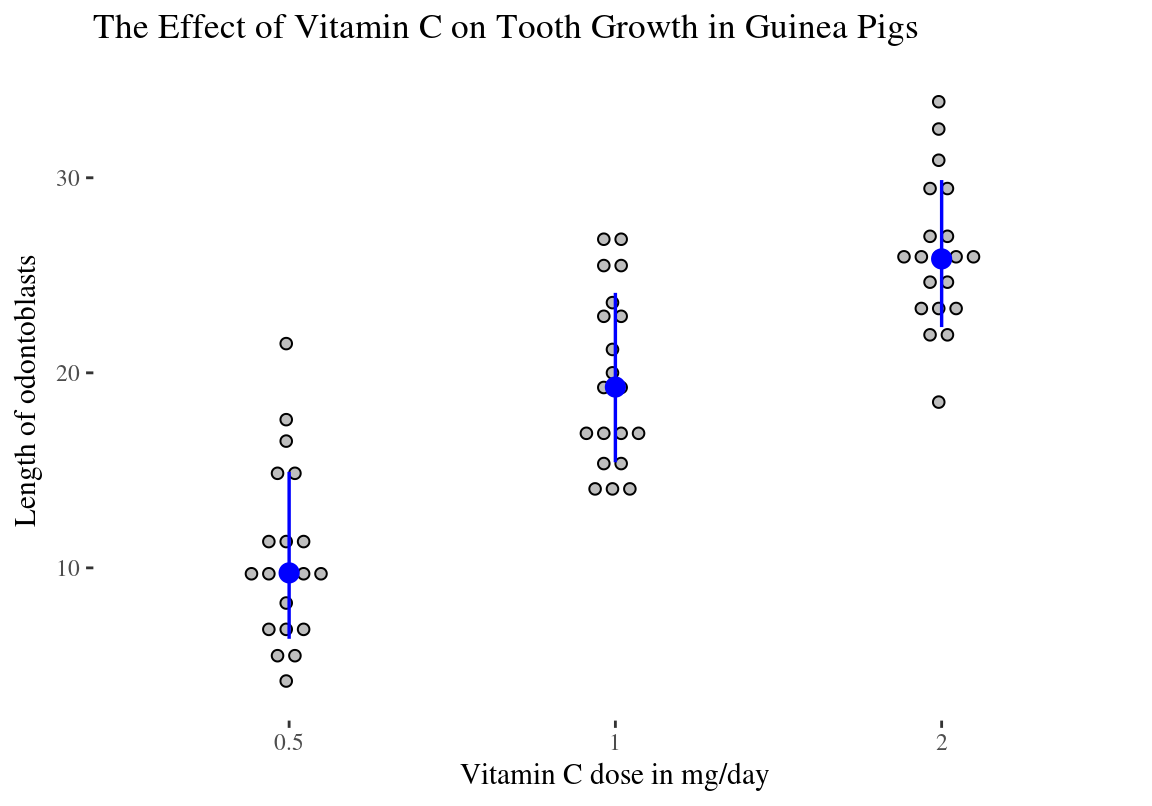
\includegraphics{07_EDA_files/figure-latex/multisd-1.pdf}
\caption{\label{fig:multisd}Multiplikatiivse sd joonistamine.}
\end{figure}

\section{EDA kokkuvõte}\label{eda-kokkuvote}

\begin{enumerate}
\def\labelenumi{\arabic{enumi}.}
\item
  Andmepunktide plottimine säilitab maksimaalselt andmetes olevat infot
  (nii kasulikku infot kui müra). Aitab leida outliereid (valesti
  sisestatud andmeid, valesti mõõdetud proove jms). Kui valim on väiksem
  kui 20, piisab täiesti üksikute andmepunktide plotist koos mediaaniga.
  Dot-plot ruulib.
\item
  Histogramm -- kõigepealt mõõtskaala ja seejärel andmed jagatakse
  võrdse laiusega binnidesse ja plotitakse binnide kõrgused. Bin, kuhu
  läks 20 andmepunkti on 2X kõrgem kui bin, kuhu läks 10 andmepunkti.
  Samas, bini laius/ulatus mõõteskaalal pole teile ette antud -- ja
  sellest võib sõltuda histogrammi kuju. Seega on soovitav proovida
  erinevaid bini laiusi ja võrrelda saadud histogramme. Histogramm
  sisaldab vähem infot kui dot plot, aga võimaldab paremini tabada
  seaduspärasid \& andmejaotust \& outliereid suurte andmekoguste
  korral.
\item
  Density plot. Silutud versioon histogrammist, mis kaotab infot aga
  toob vahest välja signaali müra arvel. Density plotte on hea kõrvuti
  vaadelda joy ploti abil.
\item
  Box-plot --- sisaldab vähem infot kui histogramm, kuid neid on lihtsam
  kõrvuti võrrelda. Levinuim variant (kuid kahjuks mitte ainus) on Tukey
  box-plot -- mediaan (joon), 50\% IQR (box) ja 1,5x IQR (vuntsid),
  pluss outlierid eraldi punktidena.
\item
  Violin plot --- informatiivsuselt box-ploti ja histogrammi vahepeal --
  sobib paljude jaotuste kõrvuti võrdlemiseks.
\item
  Line plot --- kasuta ainult siis kui nii X kui Y teljele on kantud
  pidev väärtus (pikkus, kaal, kontsentratsioon, aeg jms). Ära kasuta,
  kui teljele kantud punktide vahel ei ole looduses mõtet omavaid
  pidevaid väärtusi (näiteks X teljel on katse ja kontroll või erinevad
  valgumutatsioonid, mille aktiivsust on mõõdetud).
\item
  Tulpdiagramm -- Suhete võrdlemine (bar).
\item
  Cleveland plot on hea countide võrdlemiseks. Kui Cleveland plot mingil
  põhjusel ei sobi, kasuta tupldiagrammi.
\item
  Pie chart on proportsioonide vaatamiseks enam-vähem kõlblik ainult
  siis, kui teil pole vaja võrrelda proportsioone erinevates objektides.
  Kõik graafikud, kus lugeja peab võrdlema pindalasid, on inimmõistusele
  petlikud --- lugeja alahindab süstemaatiliselt erinevuste suurusi!
  Selle pärast on proportsioonide võrdlemiseks palju parem tulpdiagramm,
  kus võrreldavad tulbad on ühekõrgused.
\end{enumerate}

Informatsiooni hulk kahanevalt: iga andmepunkt plotitud
---\textgreater{} histogramm ---\textgreater{} density plot \& violin
plot ---\textgreater{} box plot ---\textgreater{} tulpdiagramm
standardhälvetega ---\textgreater{} cleveland plot (ilma veapiirideta)

\chapter{Lausearvutuslik loogika}\label{lausearvutuslik-loogika}

Enne, kui siirdume järeldava statistika ja tõenäosusteooria juurde,
teeme lühikese sissejuhatuse klassikalisse loogikasse, sest
tõenäosusteooria ei ole lõppude-lõpuks midagi muud, kui loogika laiendus
juhule, kus me ei ole kindlad selles, mida räägime. Niisiis, loogika
ülesanne on modelleerida inimkeelseid lauseid (või nende sisu ehk
propositsioone). Keele modelleerimise läbi modelleerime me ühtlasi
mõtlemist, kaasa arvatud teaduslik mõtlemine. Nagu ikka, ei eelda me ka
siin, et mudel vastaks täpselt reaalsusele.

Igal juhul koosneb meie keelemudeli baas-süntaks sõnadest nagu ``ja'',
``või'', ``mitte'', ``kui \ldots{} siis'', mida kutsume
\emph{konnektiivideks}.

\textbf{Konnektiivid koos neid tähistava sümboliga:}

\begin{itemize}
\item
  \emph{not} -- (\(\lnot\)) -- negatsioon e \emph{negation},
\item
  \emph{and} -- (\(\land\)) -- konjunktsioon e \emph{conjunction},
\item
  \emph{or} -- (\(\lor\)) -- disjunktsioon e \emph{disjunction},
\item
  \emph{if \ldots{} then} -- (\(\rightarrow\)) -- implikatsioon e
  konditsionaal e \emph{implication} e \emph{conditional} (if --
  \emph{antecent}, then -- \emph{consequent}).
\end{itemize}

Suured tähed A, B, C, \ldots{} tähistavad \emph{atomaarseid lauseid}.
Iga atomaarne lause tähistab ühte või mitut inimkeelset lauset. Loogiku
jaoks pole atomaarsete lausete sisemine struktuur oluline, sest sellest
ei sõltu mudelkeele lausete valiidsus.

Mudelkeele 1. tase koosneb atomaarsetest lausetest, mis on ühendatud
konnektiividega (negatsioon, konjunktsioon jne). Siin on juba tegemist
\emph{liitlausetega}. 2. taseme liitlaused koosnevad konnektiividega
ühendatud 1. taseme lausetest, ja nii edasi lõpmatusse. Näiteks
\(((A \rightarrow B) \lor (B \land A)) \rightarrow C\) on 3-tasemeline
lause, kus sulud näitavad, milliseid komponentlauseid mingi konnektiiv
parasjagu ühendab.

Lisaks konnektiividele sisaldab meie keelemudel tõeväärtusi: T ja F.
Siinkohal eeldame, et mitmetasemeliste lausete tõeväärtused sõltuvad
nende aluseks olevate atomaarsete lausete tõeväärtustest, ja mitte
millegist muust. Seda eeldust kutsutakse tõetabeli printsiibiks.

\section{Tõetabel}\label{toetabel}

Kui me tähistame suvalist liitlauset X-ga, siis tõetabel näeb välja nii:

\begin{verbatim}
#> # A tibble: 4 x 3
#>   A     B     X    
#>   <chr> <chr> <chr>
#> 1 T     F     ""   
#> 2 F     T     ""   
#> 3 T     T     ""   
#> 4 F     F     ""
\end{verbatim}

Tõetabel annab kõik võimalikud kombinatsioonid atomaarsete lausete
tõeväärtustest ja ütleb iga sellise kombinatsiooni kohta, kas X on tõene
või väär. Seega on tõetabel loogiline diagramm X-le. Tabeli iga rida
annab ühe kombinatsiooni atomaarsete lausete tõeväärtustest ja X veeru
vastavale reale peaks kirjutama X-i tõeväärtuse, mis sõltub nende
atomaarsete lausete tõeväärtusest sellel real ja sellest, milliste
konnektiividega need on liitlausesse X ühendatud. Tabeli iga rida annab
X-le unikaalse tõeväärtuse.

Kõigepealt anname tõetabeli negatsioonile, mis on unaarne konnektiiv,
ehk töötab ühe lause piires

\begin{verbatim}
#> # A tibble: 2 x 2
#>   A     `not A`
#>   <chr> <chr>  
#> 1 T     F      
#> 2 F     T
\end{verbatim}

Ehk sõnadega: \(\neg A\) on tõene siis kui \(A\) on väär, ja vastupidi.
Negatsioon ei tee muud, kui põõrab lause tõeväärtuse vastupidiseks.

\section{Konjunktsioon}\label{konjunktsioon}

Nüüd tõetabel konjunktsioonile, mis on binaarne konnektiiv, ühendades
kahte lauset.

\begin{verbatim}
#> # A tibble: 4 x 3
#>   A     B     `A and B`
#>   <chr> <chr> <chr>    
#> 1 T     T     T        
#> 2 T     F     F        
#> 3 F     T     F        
#> 4 F     F     F
\end{verbatim}

Ehk sõnadega: \(A \land B\) on tõene siis ja ainult siis kui A ja B on
mõlemad tõesed.

Konjunktsiooni võib kasutada näiteks nii:

P1 (Premiss 1): Seda ja teist

J1 (Järeldus 1): Seda

J2: teist

Või:

P1: ei ole külm ega tuuline

J1: ei ole külm

J2: ei ole tuuline

Aga lausest \(\neg (A \land B)\) ei saa midagi järeldada:

P1: Ma ei ole praegu Pariisis ega Tallinnas

J1: ---

\section{Disjunktsioon}\label{disjunktsioon}

Nüüd disjunktsioon. Loogikute jaoks on siin tegemist nn inklusiivse
või-ga, mis tähendab, et see kehtib ka siis, kui A ja B mõlemad
kehtivad.

\begin{verbatim}
#> # A tibble: 4 x 3
#>   A     B     `A or B`
#>   <chr> <chr> <chr>   
#> 1 T     T     T       
#> 2 T     F     T       
#> 3 F     T     T       
#> 4 F     F     F
\end{verbatim}

\(A \lor B\) on väär siis ja ainult siis, kui A ja B on mõlemad väärad.

Kuidas aga oleks lood ekslusiivse disjunktsiooniga (\emph{xor}), kus A =
T ja B= T viivad väärale disjunktsioonile? Me ei vaja xor jaoks
tingimata eraldi konnektiivi (sümbolit), sest selle tõetabel langeb
kokku lause \[(A \lor B) \land \neg (A \land B)\] tõetabeliga.

Selle arvutamiseks evalueerime kõigepealt sisemise disjunktiooni
\(A \lor B\) ja konjunktsiooni \(A \land B\), seejärel negatsiooni
\(\neg (A \land B)\) ja lõpuks kogu lause (see on tabelis kaskel olev
``and'').

\begin{verbatim}
#> # A tibble: 4 x 6
#>   A     B     `A or B (I)` `and (III)` `not (II)` `A and B (I)`
#>   <chr> <chr> <chr>        <chr>       <chr>      <chr>        
#> 1 T     T     T            F           F          T            
#> 2 T     F     T            T           T          F            
#> 3 F     T     T            T           T          F            
#> 4 F     F     F            F           T          F
\end{verbatim}

Tabeli evalueerimise järjekord on antud rooma numbritega tabeli veergude
päistes.

Ja võrdluseks A xor B tõetabel

\begin{verbatim}
#> # A tibble: 4 x 3
#>   A     B     `A xor B`
#>   <chr> <chr> <chr>    
#> 1 T     T     F        
#> 2 T     F     T        
#> 3 F     T     T        
#> 4 F     F     F
\end{verbatim}

Kuna nende tabelite läbiarvutamisel saadud tõeväärtused on identsed, on
laused \((A \lor B) \land \neg (A \land B) \Leftrightarrow A ~ xor ~B\)
\emph{loogiliselt ekvivalentsed}. Ekvivalentsed võivad olla ka laused,
mis ei koosne samadest atomaarlausetest, senikaua kui nende tõetabeli
kõik read on sama tõeväärtusega (näiteks A ja \(A\land(B\lor\neg B\))).

Disjunktsiooni ja konjunktsiooni on võimalik avaldada teineteise kaudu:

\[\neg (A \land B) \Leftrightarrow \neg A \lor \neg B\]

\[\neg (A \lor B) \Leftrightarrow \neg A \land \neg B\]

Disjunktsiooni saab kasutada näiteks nii:

P1: Ei seda ega teist (\(\neg (A \lor B)\))

J1: Ei seda (\(\neg A\))

J2: ei teist (\(\neg B\))

Või

P1: ei mitte-A ega mitte-B (\(\neg (\neg A \lor \neg B)\))

J1: A

J2: B

Samas, lausest \(A \lor B\) ei saa midagi järeldada:

P1: Ma olen kas Pariisis või Tallinnas

J1: ----

\section{Konditsionaal}\label{konditsionaal}

Ja lõpuks konditsionaali \(A \rightarrow B\) tõetabel

\begin{verbatim}
#> # A tibble: 4 x 3
#>   A     B     `if A then B`
#>   <chr> <chr> <chr>        
#> 1 T     T     T            
#> 2 T     F     F            
#> 3 F     T     T            
#> 4 F     F     T
\end{verbatim}

Konditsionaal on väär siis ja ainult siis kui A on tõene ja B on väär.
Vahest kipuvad inimesed nägema konditsionaali põhjusliku seose mudelina.
See ei ole aga hea mõte, sest loogilised tehted eeldavad ainult koos või
eraldi esinemist, mitte põhjuslikke ega ajalisi suhteid.

Veel üks oluline samasus:
\[A \rightarrow B \Leftrightarrow \neg B \rightarrow \neg A\].

Lisaks võime konditsionaali avaldada ka läbi disjunktsiooni või
konjunktsiooni:
\[A \rightarrow B \Leftrightarrow \neg A \lor B \Leftrightarrow \neg(A \land B)\].
Ainus põhjus, miks meil on eraldi konnektiiv nimega konditsionaal, on
selle järeldusliku vormi sage kasutamine. Seega on konditsionaal
loogikas sisuliselt vähetähtis mugavussümbol, mitte põhjusliku seose
sügavmõtteline mudel.

Konditsionaali \(A \rightarrow B\) osaline vaste tõenäosusteoorias on
tingimuslik tõenäosus \(P(B ~\vert~ A)\), mis ütleb ``B tõenäosus
tingimusel, et A on tõene'' (vt allpool).

Konditsionaali saab kasutada näiteks nii

P1: \(\neg (A \rightarrow B)\)

J1: \(A\)

J2: \(\neg B\)

Jällegi, lausest \(A \rightarrow B\) ei saa midagi järeldada A ega B
kohta.

P1: \(A \rightarrow B\)

J1: ---

\section{Tautoloogia ja
kontradiktsioon}\label{tautoloogia-ja-kontradiktsioon}

\(A \lor \neg A\) on tautoloogia, sest selle tõetabelis on X alati tõene

\begin{Shaded}
\begin{Highlighting}[]
\KeywordTok{tibble}\NormalTok{(}\DataTypeTok{A =} \KeywordTok{c}\NormalTok{(}\StringTok{"F"}\NormalTok{, }\StringTok{"T"}\NormalTok{), }\StringTok{`}\DataTypeTok{A or notA}\StringTok{`}\NormalTok{ =}\StringTok{ }\KeywordTok{c}\NormalTok{(}\StringTok{"T"}\NormalTok{, }\StringTok{"T"}\NormalTok{))}
\CommentTok{#> # A tibble: 2 x 2}
\CommentTok{#>   A     `A or notA`}
\CommentTok{#>   <chr> <chr>      }
\CommentTok{#> 1 F     T          }
\CommentTok{#> 2 T     T}
\end{Highlighting}
\end{Shaded}

Tautoloogiast tuleneb välistatud kolmanda seadus, mille kohaselt iga
propositsioon on kas tõene või väär (ja mitte kunagi mõlemat korraga).

Seevastu \(A \land \neg A\) on kontradiktsioon ehk iseendaga
vastuoluline ehk loogiliselt vastuoluline, sest selle tõetabelis on X
alati väär.

\begin{Shaded}
\begin{Highlighting}[]
\KeywordTok{tibble}\NormalTok{(}\DataTypeTok{A =} \KeywordTok{c}\NormalTok{(}\StringTok{"F"}\NormalTok{, }\StringTok{"T"}\NormalTok{), }\StringTok{`}\DataTypeTok{A and notA}\StringTok{`}\NormalTok{ =}\StringTok{ }\KeywordTok{c}\NormalTok{(}\StringTok{"F"}\NormalTok{, }\StringTok{"F"}\NormalTok{))}
\CommentTok{#> # A tibble: 2 x 2}
\CommentTok{#>   A     `A and notA`}
\CommentTok{#>   <chr> <chr>       }
\CommentTok{#> 1 F     F           }
\CommentTok{#> 2 T     F}
\end{Highlighting}
\end{Shaded}

Nagu juba eespool mainitud, kui tõetabelis leidub rida, kus kõik
atomaarsed laused on tõesed ja X on väär, siis ja ainult siis on tegu
kontradiktsiooniga. Antud juhul on selline tabeli 2. rida

\section{loogiline argument ja valiidne
järeldamine}\label{loogiline-argument-ja-valiidne-jareldamine}

Näiteks lause: maa on kerakujuline või kuu on juustust. Nüüd eeldame, et
maa ei ole kerakujuline. Siit tuleb loogiliselt valiidne järeldus: kuu
on juustust.

Ehk

P1: AvB

P2: mitte-A

J: B

Siin on meil tegemist loogilise \textbf{argumendiga}, mis koosneb kahest
\textbf{premissist} (P1 ja P2) ja järeldusest (J). Premissid on laused,
mille kohta me eeldame, et need on tõesed, ja järelduse me dedutseerime
premissidest lähtuvalt sellest eeldusest.

Mis juhtub, kui me eeldame, et järeldus B on hoopiski väär, aga
premissid mitte-A ja AvB on mõlemad tõesed? Sellisel juhul on meil tegu
loogilise vastuolu e kontradiktsiooniga. Seega on premissidest
dedutseeritud järeldus loogiliselt tõsikindel; iga deduktiivne järeldus
on juba peidus premissides ja ei sisalda endas uut informatsiooni.

Järelduse loogiline valiidsus ei taga selle kehtivust päris maailmas
(kui tagaks, siis me elaksime vaid matemaatikast koosnevas maailmas,
mille mõistmiseks poleks vaja teha empiirilisi uuringuid). Me võime sama
hästi eeldada, et (P1) maa on kerakujuline või kuu on juustust e AvB,
(P2) et kuu ei ole juustust e mitte-B, ja siit järeldub, et maa on
kerakujuline:

AvB

mitte-B

J: A,

See järeldus on nii valiidne kui kehtiv. Aga samas empiiriliselt mitte
kuigi huvitav.

\begin{quote}
Argument on \textbf{valiidne} siis ja ainult siis, kui olukord, kus kõik
premissid oleksid tõesed ja järeldus oleks väär, on loogiliselt
vastuoluline. Argument on \textbf{kehtiv} (\emph{sound}) siis ja ainult
siis, kui see on valiidne ja kõik premissid on tõesed.
\end{quote}

Argumendi valiidsus tähistab pelgalt argumendi korrektset semantilist
struktuuri (ehk loogilist vormi). Argumendi kehtivus tähendab, et
argumendi järeldus on ka sisuliselt kehtiv ehk tõene. Valiidne
järeldamine eeldab, et premissid ja järeldus on ehitatud atomaarsetest
lausetest nii, et ei esine atomaarsete lausete tõeväärtuste
kombinatsiooni, mis muudaks kõik premissid tõeseks ja järelduse vääraks.
Kui siiski esineb selline kombinatsioon, siis oleme leidnud loogilise
vastuolu ehk kontradiktsiooni ja meie järeldamismehhanism ei saa olla
valiidne.

Selle näitlikustamiseks kontrollime argumendi

P1: \(A \rightarrow B\)

P2: \(\neg A\)

J: \(\neg B\)

valiidsust tõetabeli abil:

\begin{Shaded}
\begin{Highlighting}[]
\KeywordTok{tibble}\NormalTok{(}\DataTypeTok{A=}\KeywordTok{c}\NormalTok{(}\StringTok{"T"}\NormalTok{, }\StringTok{"T"}\NormalTok{, }\StringTok{"F"}\NormalTok{, }\StringTok{"F"}\NormalTok{), }\DataTypeTok{B=}\KeywordTok{c}\NormalTok{(}\StringTok{"T"}\NormalTok{, }\StringTok{"F"}\NormalTok{, }\StringTok{"T"}\NormalTok{, }\StringTok{"F"}\NormalTok{), }\StringTok{`}\DataTypeTok{P1: if A then B}\StringTok{`}\NormalTok{=}\StringTok{ }\KeywordTok{c}\NormalTok{(}\StringTok{"T"}\NormalTok{, }\StringTok{"F"}\NormalTok{, }\StringTok{"T"}\NormalTok{, }\StringTok{"T"}\NormalTok{), }\StringTok{`}\DataTypeTok{P2: notA}\StringTok{`}\NormalTok{=}\StringTok{ }\KeywordTok{c}\NormalTok{(}\StringTok{"T"}\NormalTok{, }\StringTok{"F"}\NormalTok{, }\StringTok{"T"}\NormalTok{, }\StringTok{"T"}\NormalTok{), }\StringTok{`}\DataTypeTok{J: notB}\StringTok{`}\NormalTok{=}\StringTok{ }\KeywordTok{c}\NormalTok{(}\StringTok{"T"}\NormalTok{, }\StringTok{"T"}\NormalTok{, }\StringTok{"F"}\NormalTok{, }\StringTok{"T"}\NormalTok{)) }\CommentTok{#%>% kableExtra::kable()}
\CommentTok{#> # A tibble: 4 x 5}
\CommentTok{#>   A     B     `P1: if A then B` `P2: notA` `J: notB`}
\CommentTok{#>   <chr> <chr> <chr>             <chr>      <chr>    }
\CommentTok{#> 1 T     T     T                 T          T        }
\CommentTok{#> 2 T     F     F                 F          T        }
\CommentTok{#> 3 F     T     T                 T          F        }
\CommentTok{#> 4 F     F     T                 T          T}
\end{Highlighting}
\end{Shaded}

Tõetabelist on näha, et see argument ei ole valiidne, sest tabeli 3.
reas on tõesed premissid ja väär järeldus. Nii lihtne see ongi. Pane
tähele, et sellises tõetabelis on huvitavad ainult sellised read, kus
ükski premiss pole väär ja järeldus on väär. Kõiki teisi ridu võib
ignoreerida. Kuna tabeli ridade arv võrdub kaks astmes atomaarsete
lausete arv, milline number kasvab atomaarsete lausete arvu kasvuga väga
kiiresti, tasub seda meeles pidada.

\section{Modus Ponens ja Modus
Tollens}\label{modus-ponens-ja-modus-tollens}

Bertrand Russelile, kellel on väga suured teened formaalse loogika
arendamisel 20. sajandi alguses, kuulub väike nali teadusliku meetodi
kohta, nagu seda nägid paljud 20. sajandi teadusfilosoofid (Russell,
1945):

\begin{verbatim}
If p, then q; now q is true; therefore p is true. 
E.g. if pigs had wings then some winged animals 
are good to eat; therefore pigs have wings. 
This form of inference is called `scientific method`.
\end{verbatim}

See inglise huumor näitlikustab induktiivset teadusliku mõtlemise
mudelit, mis ekslikult kasutab deduktiivse lausearvutusliku süllogismi
mitte-valiidset vormi. Tegemist on sedavõrd levinud eksitusega, et
sellel on lausa oma ladinakeelne nimi, mida võib tõlkida kui ``peale
seda, järelikult selle pärast'' (\emph{Post hoc ergo propter hoc}).
Selle süllogismi vähem naljakas rakendus oleks:

P1: Kui patsiendil on gripp, siis on tal (tõenäoliselt) palavik
{[}\(A \rightarrow B\){]}

P2: palavik {[}B{]}

J1: gripp {[}A{]}

J2: tõenäoliselt gripp {[}P(A) on kõrge{]}

Paraku kumbki järeldus ei kehti.

Teine ja palju kavalam katse lausearvutusliku loogika abil teaduslikku
mõtlemist mudeldada kuulub teadusfilosoof Karl Popperile. Et Popperi
mudelit tutvustada, alustame valiidsest (ehkki mitte tingimata
kehtivast) deduktiivsest argumendist ladinakeelse nimega \emph{Modus
Ponens}

P1: \(A \rightarrow B\)

P2: \(A\)

J: \(B\)

Ehk,

P1: kõik mehed on sead (kui mees, siis siga)

P2: Aristoteles on mees

J: Aristoteles on siga

Et modelleerida üldist ja alati kehtivat loodusseadust, mis oli Popperi
jaoks teaduslik teooria par excellence, seondub selle argumendiga
probleem, millest oli teadlik juba Aristoteles. Kui me tahame
tõsikindlalt näidata, et kõik mehed on tõepoolest sead, siis peame
minema induktiivset rada ja testima tõepoolest kõiki mehi, nii praegusi,
eilasi, kui homseid selles osas, kui palju nad sigu meenutavad.

P1: 1. mees on siga

P2: 2. mees on siga

\ldots{}..

Pn: n-s mees on siga

J: Kõik mehed on sead

See ei ole paraku teostatav.

Popper püüdis probleemi lahendada, tuues sisse valiidse deduktiivse
argumendi vormis \emph{Modus Tollens}:

P1: \(A \rightarrow B\)

P2: \(\neg B\)

J: \(\neg A\)

ehk:

P1: kõik mehed on sead

P2: Aristoteles ei ole siga

J: Aristoteles ei ole mees

Aga seda võib vaadata ka nii: Kui me eeldame, et Aristoteles siiski on
mees, ja et Aristoteles ei ole siga, siis argumendi valiidsuse
päästmiseks teeme järelduse, et P1 on väär (st kõik mehed ei ole teps
mitte sead). Sellisel viisil loogilise vastuolu lahendamine on täiesti
lubatud ja soositud tegevus.

Seega oli Popperi retsept teadlastele (loe: füüsikutele)

\begin{enumerate}
\def\labelenumi{\arabic{enumi}.}
\item
  postuleeri üldine teooria vormis: kõik X-d on Y.
\item
  Dedutseeri sellest mõni teaduslikult testitav alamteooria vormis
  \(x_i\) on Y.
\item
  Juhul kui me suudame empiiriliselt näidata, et see alamteooria on
  väär, oleme sellega deduktiivselt ümber lükanud ka üldise teooria
  kehtimise.
\end{enumerate}

Seda skeemi illustreerib hästi Enrico Fermi tsitaat:

\begin{verbatim}
If your experiments succeed in provig the hypothesis, 
you have made a measurement; if they fail to prove 
the hypothesis, you have made a discovery.
\end{verbatim}

Sellist suure teooria ümber lükkamist kitsama haardega alamteooria
testimise läbi nimetatakse teooria falsifitseerimiseks. Siit tuleneb ka
Popperi ettepanek teaduse ja mitte-teaduse eristamiseks: kõik
teaduslikud teooriad peavad olema vähemalt põhimõtteliselt
falsifitseeritavad (sest muidu ei saaks neid Popperi teadusliku
mõtlemise mudeli abil ümber lükata), millest tuleneb omakorda, et mida
lihtsam on teooriat falsifitseerida, seda ``teaduslikum'' see teooria
on. Näiteks teooria, mille kohaselt igal kolmapäeval kell 14:00 sajab
Ilmatsalu ilmajaamas 3 mm õllevihma, on suurepäraselt falsifitseeritav
ja seega super-teaduslik. Igal juhul lõi Popper kõigepealt teadusliku
mõtlemise formaalse mudeli ja teatas seejärel, et kuna see mudel töötab
ainult teatud struktuuriga teooriate peal, siis kallid teadlased, palun
ajage oma teooriad õigesse vormi või leppige sildiga
``mitte-teaduslik''.

Teine häda oli see, et alamteooria ümber lükkamiseks viisil, mis
kindlustab Modus tollensi kehtimise, peame olema absoluutselt kindel, et
me oleme selle päriselt ümber lükanud. Seega peame oleme täiesti
kindlad, et meie katseaparatuur teeb seda, mida me tahame, et
mõõtmisviga ei vii meid ekslikele järeldustele jne. Popperil oli selle
vastuväite osas öelda seda, et olgu peale, me peame kasutama eeldusi,
mille kehtimises me ei saa kindlad olla, aga vähemalt põhimõtteliselt
oleme me nõus iga sellise eelduse avama ja läbi vaatama, kui selleks
peaks vajadus tekkima. Senikaua kui see on nii, on Popperi järgi tegu
teadusega. Seega me eeldame, et Modus Tollens töötab nagu kellavärk, aga
ainult mõtlemise mudeli piires. Tegelikus teaduslikus praktikas ei saa
siiski millegile kindel olla!

Falsifitseerimise kui teadusliku mõtlemise mudeli põhiline ja ületamatu
puudus on, et see töötab lausearvutusliku loogika raames, mis tähendab,
et see jääb paratamtult hätta teooriatega, mis ennustavad millegi
juhtumist tõenäosuslikult. Näiteks teooria, mille kohaselt suitsetamine
põhjustab kopsuvähki, aga mitte igal suitsetajal (suitsetamise põhiline
suremust tõstev mõju on läbi südamehaiguste, mitte vähi). Lausearvutuses
ei ole ühtegi mehhanismi tõenäosuslike propositsioonidega töötamiseks ja
Popperi, kes oli mõnede arvates oma põlvkonna nutikaim filosoof, 70
aastat kestnud pingutused selline mehhanism luua jooksid liiva.

\section{Lausearvutusest tõenäosuste
loogikasse}\label{lausearvutusest-toenaosuste-loogikasse}

Mis juhtub, kui meie premiss ei ole mitte ``kuu on tehtud juustust''
vaid ``kuu on võib-olla tehtud juustust'', ehk ``meil on andmeid, et kuu
on tehtud juustust'', ehk ``kuu on tõenäoliselt tehtud juustust''?
Sellisel juhul ei ole loogiline järeldus ``A'' ehk ``A = TRUE'', vaid
hoopis ``võib-olla A'' ehk ``tõenäoliselt A'' ehk ``P(A) = {[}reaalarv 0
ja 1 vahel{]}''. Lausearvutuse reeglid eeldavad, et premissid on kas
tõesed või väärad, ehk premisside (ja järelduste) tõenäosused tohivad
omada vaid kahte väärtust: 1 ja 0. Seega ei saa me siin lausearvutust
rakendada ja vajame teistsugust loogikat, mis võimaldaks ebakindlate
premisside põhjal teha ebakindlaid järeldusi. See tähendab, et me vajame
tõenäosusteooriat.

Kui lausearvutus töötab must-valges tõene-väär maailmas, siis
tõenäosusteooria opereerib halli varjunditega. Tõenäosusteoorialt kui
loogika laienduselt ootame, et see annaks meile järeldused kujul ``A
tõenäosus'' (P(A)) või ``A tõenäosus, juhul kui kehtib B'' (P(A I B)).
Lisaks ootame, et alati, kui tõenäosused on fikseeritud ühe ja nulliga,
annaks tõenäosusteooria välja samad järeldused kui lausearvutus.
Üldiselt tahame me mõlema loogika puhul sama: konverteerida premissid
parimateks võimalikeks järeldusteks, mida saaksime (küll mingil määral
ja mööndustega) formaalse mudeli maailmast ka päris maailma üle kanda.

Lausearvutus on deduktiivne süsteem, kus järelduse tõesus sisaldub juba
premissides. Kui loogik on tõese järelduseni jõudnud, siis see järeldus
on igavene -- seda ei saa muuta uusi premisse või andmeid lisades. Seda
omadust nimetatakse loogika monotoonilisuseks. Teisisõnu,
lausearvutuslik loogika on mõtlemise mudel, mis ei sisalda kahtlusi ega
isegi võimalust kahtlusteks. Selline mudel ei ole ilmselgelt see, mida
otsib teadlane, kes peab oma järeldusi tegema mittetäieliku
informatsiooni tingimustes.

Tõenäosusteooria on matemaatika haruna deduktiivne aksiomaatiline
süsteem, aga mõtlemise mudelina kasutatakse seda hoopiski induktiivsel
moel. See tähendab, et me püüame piiratud andmete põhjal jõuda
ebakindlatele järeldustele, aga seejuures seda ebakindlust tõenäosustega
kvantifitseerides. Uusi andmeid lisades saame me oma episteemilise
ebakindluse (``episteemiline ebakindlus'' tähendab, et segadus asub meie
peas, mitte maailma ülesehituses) määra muuta, aga ainus viis saavutada
tõsikindlust (ja monotoonilisust), on tuues arvutusse sisse null- ja
ühiktõenäosused. Seega on tõenäosusteooriat mõtlemise mudelina
rakendades teaduslikus praktikas üsna võimatu jõuda tõsikindlatele
järeldustele. Ja inimesed, kes teaduses opereerivad lausearvutusliku
loogikaga (ja seega ei mõtle tõenäosuslikult), eeldavad vaikimisi, et
nende jaoks on teadus matemaatikat meenutav tõsikindel süsteem, mis oma
sisendites (katseskeemid, andmed, nende analüüs) ei sisalda ebakindlust.
Samas, ka meie, kes me kasutame tõenäosusteooriat, peame eeldama, et see
on vaid mõtlemise mudel, mitte teaduslik mõtlemine ise oma ehedal kujul.
Kohe, kui keegi mõtleb välja parema mudeli, hakkame kõik kasutama seda.
Aga senikaua peame õppima tõenäosusteooriat ja selle praktilist
edasiarendust, mida kutsume Bayesi statistikaks.

\chapter{Järeldav statistika}\label{jareldav-statistika}

Kui EDA määrab graafiliste meetoditega andmete kvaliteeti ja püstitab
uusi hüpoteese, siis järeldav statistika püüab formaalsete arvutuste
abil vastata kahele lihtsale küsimusele: 1. mis võiks olla kõige
usutavam parameetriväärtus? ja 2. kui suur ebakindlus seda hinnangut
ümbritseb? Kuna andmed tulevad meile lõpliku suurusega valimina koos
mõõtmisveaga ja bioloogilise varieeruvusega, on ebakindlus hinnagusse
sisse ehitatud. Hea protseduur kvantifitseerib selle ebakindluse ausalt
ja täpselt -- siin ei ole eesmärk niivõrd mitte ebakindlust vähendada
(seda teeme eelkõige katse planeerimise tasemel), vaid seda kirjeldada.
Järeldav statistika püüab, kasutades algoritme ja mudeleid, teha andmete
põhjal järeldusi looduse kohta.

\begin{quote}
Ebakindluse allikad on mõõtmisviga, bioloogiline varieeruvus, mudeli
viga (matemaatiline jaotusfunktsioon ei vasta looduses toimuvale),
algoritmi viga (algoritm ei tee seda, mida kasutaja tahab) ja
süstemaatiline viga (juhtub, kui te saate valesti aru oma
katsesüsteemist, harrastate teaduslikku pettust või teete kõike muud,
mis kallutab teie andmeid). Süstemaatilist viga ei saa kunagi välistada
-- see on loogiline paratamatus, mis tuleneb asjaolust, et andmeid on
alati vähem kui on võimalikke süstemaatilise vea allikaid (ja sest
lisaks ei ole meil kunagi täielikku nimekirja võimalikest vea
allikatest), mille vahel saab loogiliselt vahet teha ainult neidsamaseid
andmeid kasutades. Seega on vea allikad, millest igaüks on vaadeldav
eraldiseisva alternatiivse teadusliku hüpoteesina meie põhihüpoteesile,
andmete poolt loogiliselt alamääratud, mis tähendab et kindel teadmine
teaduses on loogiliselt võimatu. Seega ulatuvad teaduslikud hüpoteesid
alati teistpoole andmeid, ehk need ütlevad rohkem, kui oleks võimalik
puhtalt andmete põhjal õigustada, ja sisaldavad usukomponenti. See on
üks põhjus, miks me sõandame riskida mudelite kasutamisega oma
hüpoteeside kinnitamisel.
\end{quote}

Sellisel tegevusel on mõtet ainult siis, kui ühest küljest andmed
peegeldavad tegelikkust ja teisest küljest tegelikkus hõlmab enamat, kui
lihtsalt meie andmeid. Kui andmed = tegelikkus, siis pole mõtet
keerulisi mudeleid kasutada -- piisab lihtsast andmete kirjeldusest. Ja
kui andmetel pole midagi ühist tegelikkusega, siis on need lihtsalt
ebarelevatsed. Seega on järeldava statistika abil tehtud järeldused
alati rohkem või vähem ebamäärased ning meil on vaja meetodit selle
ebamäärasuse mõõtmiseks. Selle meetodi annab tõenäosusteooria.

\section*{Järeldav statistika on tõenäosusteooria
käepikendus}\label{jareldav-statistika-on-toenaosusteooria-kaepikendus}
\addcontentsline{toc}{section}{Järeldav statistika on tõenäosusteooria
käepikendus}

See õpik õpetab Bayesi statistikat, mis põhineb tõenäosusteoorial. Tänu
sellele moodustab Bayesi statistika sidusa terviku, mille abil saab teha
kõike seda, mida saab teha tõenäosusteooria abil. Bayesi statistika
põhineb Bayesi teoreemil, mis on triviaalne tuletus tõenäosusteooria
aksioomidest. Tänu Cox-i teoreemile (1961) teame, et klassikaline
lausearvutuslik loogika on tõenäosusteooria erijuht ning, et Bayesi
teoreem on teoreetiliselt parim viis tõenäosustega töötamiseks. Seega,
kui te olete kindel oma väidete tõesuses või vääruses, siis on
klassikaline loogika parim viis nendega opereerida; aga kui te ei saa
oma järeldustes päris kindel olla, siis on teoreetiliselt parim lahendus
tõenäosusteooria ja Bayesi teoreem.

\begin{verbatim}
Lisaks kooskõlalisusele tõenäosusteooriaga eristab Bayesi statistikat 
klassikalisest sageduslikust statistikast kaks põhilist asjaolu: Bayesis 
kasutatakse episteemilist tõenäosuse tõlgendust, mille kohaselt tõenäosus 
mõõdab usu määra hüpoteesi kehtimisse, ja teiseks, iga Bayesi arvutus 
sisaldab lisaks andmetele meie neist andmetest sõltumatut hinnangut hüpoteesi
kehtimise tõenäosusele (see hinnang on formaliseeritud nn eeljaotuses ehk
eeltõenäosuses ehk prioris). Ortodoksne nn sageduslik statistika kasutab 
seevastu nn objektiivset ehk sageduslikku tõenäosuse tõlgendust ja ei kasuta
eeltõenäosusi oma arvutustes. Põhjalikumat seletust vt allpool ja lisa 1.
\end{verbatim}

Tõenäosusteooria on aksiomaatiline süsteem, mille abil saame omistada
numbriline väärtuse meie usu määrale mingisse hüpoteesi. Näiteks, kui me
planeerime katset, kus me viskame kulli ja kirja ja teeme seda kaks
korda, siis saame arvutada, millise tõenäosusega võime oodata katse
tulemuseks kaht kirja. Aga seda tingimusel, et me võtame omaks mõned
eeldused -- näiteks et münt on aus ja et need kaks viset on üksteisest
sõltumatud.

Sellel katsel on 4 võimalikku tulemust: H-H, H-T, T-H, T-T (H - kull, T
- kiri). Tõenäosus saada 2-l mündiviskel 2 kirja, P(2 kirja) = 1/4, P(0
kirja) = 1/4 ja P(1 kiri) = 2/4 = 1/2. Sellega oleme andnud oma
katseplaanile täieliku tõenäosusliku kirjelduse (pane tähele, et 1/4 +
1/4 + 1/2 = 1). Ükskõik kui keeruline on teie katseplaan,
põhimõtteliselt käib selle tõenäosusteoreetiline analüüs samamoodi.
Tõenäosusteooria loomus seisneb kõikide võimalike sündmuste
üleslugemises ja erinevat tüüpi sündmuste suhteliste sageduste
arvutamises -- ning senikaua, kui me seda nüri järjekindlusega teeme, on
vastus, mille me saame, tõsikindel.

Ehkki Bayesi statistika põhineb tõenäosusteoorial ja on sellega
kooskõlas, ei ole see sama asi, mis tõenäosusteooria. Statistikas
pööratakse tõenäosusteoreetiline ülesanne pea peale ja küsitakse nii:
kui me saime 2-l mündiviskel 2 kirja, siis millise tõenäosusega on münt
aus (tasakaalus)? Erinevus tõenäosusteoreetilise ja statistilise
lähenemise vahel seisneb selles, et kui tõenäosusteoorias me eeldame, et
teame, kuidas süsteem on üles ehitatud, ja ennustame sellest lähtuvalt
võimalike (hüpoteetiliste) andmete tõenäosusi, siis statistikas me
kontrollime neid eeldusi päriselt olemasolevate andmete põhjal. Seega
annab tõenäosusteooria matemaatiliselt tõsikindlaid vastuseid
ideaalmaailmade kohta, samas kui statistika püüab andmete põhjal teha
järeldusi päris maailma kohta. Selleks kasutame Bayesi teoreemi (vt
allpool).

\begin{quote}
Tõenäosusteooria määrab kõikide võimalike sündmuste esinemise
tõenäosused, eeldades, et hüpotees H kehtib (H on siin lihtsalt teine
nimi ``eeldusele'').
\end{quote}

\begin{quote}
Statistika hindab H-i kehtimise tõenäosuse lähtuvalt kogutud andmetest,
matemaatilistest mudelitest ning taustateadmistest.
\end{quote}

\textbf{Tõenäosusteooria aksioomid on tuletatavad järgmistest
eeldustest}:

\begin{itemize}
\item
  hüpoteesi usutavuse määra saab kirjeldada reaalarvudega 0 ja 1 vahel
\item
  ratsionaalne mõtlemine vastab kvalitatiivselt tervele mõistusele:
  tõendusmaterjal hüpoteesi toetuseks tõstab selle hüpoteesi usutavust.
\item
  mõtlemine peab olema konsistentne: kui me saame järeldusi teha rohkem
  kui ühel viisil, peame lõpuks ikkagi alati samale lõppjäreldusele
  jõudma
\item
  kogu kättesaadav relevantne informatsioon tuleb järelduste tegemisel
  arvesse võtta (totaalse informatsiooni printsiip)
\item
  ekvivalentsed teadmised on representeeritud ekvivalentsete numbritega.
\end{itemize}

\textbf{Tõenäosusteooria aksioomid}, mida on neli tükki, ütlevad tõlkes
inimkeelde,

\begin{enumerate}
\def\labelenumi{(\arabic{enumi})}
\item
  et iga sündmuse tõenäosus on suurem või võrdne nulliga -
  \(P(A) \geq 0\),
\item
  et loogiliselt paratamatu sündmuse tõenäosus on üks - \(P(\Omega)=1\).
  \(\Omega\) on \emph{sample space}, mis koosneb üksteist välistavatest
  ja ammendavatest hüpoteesidest. Nende hüpoteeside tõenäosuste summa on
  1, mis tähendab, et täpselt üks neist kehtib paratamatult.
\item
  et üksteist välistavate sündmuse puhul võrdub tõenäosus, et toimub üks
  või teine sündmus, nende sündmuste tõenäosuste summaga, ehk
  \(P(A \lor B) = P(A) + P(B)\).
\item
  et sündmuse A tõenäosus, juhul kui me eeldame sündmuse B kehtimist,
  võrdub nende kahe sündmuse koosesinemise tõenäosuse jagatisega
  sündmuse B tõenäosusest, ehk
  \(P(A~\vert~B) = \frac{P(A \land B)}{P(B)}\).
\end{enumerate}

Sümbolite tähendused:

\begin{itemize}
\item
  \(A \land B\) tähendab ``A ja B'',
\item
  \(A \lor B\) tähendab ``A või B'',
\item
  \(\lnot A\) tähendab mitte-A, ehk A == FALSE.
\item
  \(P(A~ \vert ~B)\) on tinglik tõenäosus, mida tuleks lugeda: ``A
  tõenäosus tingimusel, et kehtib B''. Sellega me ei väida, et B
  päriselt kehtib, vaid küsime: ``Kui peaks juhtuma, et B kehtib,
  milline oleks sellisel juhul A tõenäosus?''. Pane tähele, et
  \(P(vihm~\vert~pilves~ilm)\) ei ole numbriliselt sama, mis
  \(P(pilves~ilm~\vert~vihm)\).
\end{itemize}

Need aksioomid, mis oma matemaatilises vormis postuleeriti Andrei
Kolmogorovi poolt ca 1933, peaksid olema iseenesestmõistetavad ja ainult
neist on tuletatud kogu tõenäosusteooria. Tõenäosusteooria on
matemaatika haru, mis tähendab, et sümbolitel P, A, B, jms ei ole selles
muud fikseeritud tähendust, kui et need käituvad vastavalt
tõenäosusteooria aksioomidele ja neist dedutseeritud teoreemidele.
Nendes piirides võime anda neile sümbolitele anda ükskõik millise
tähenduse, mis siis seob matemaatilise struktuuri päris maailmaga, mis
ei ole oma loomuselt matemaatiline formalism. Näiteks \(P(A~\vert~B)\)
võib tähendada ``hüpoteesi A tõenäosust tingimusel, et meil on andmed
B'', aga sama hästi ka ``andmete A tõenäosust tingimusel, et kehtib
hüpotees B'', või ka midagi muud. \(P(A)\) võib meie jaoks tähistada
``hüpoteesi tõenäosust'', ``andmete tõenäosust'', ``tõendusmaterjali
tõenäosust'' ja ``sündmuse tõenäosust'', aga ka ``homse vihma
tõenäosust'' või ``tõenäosust, et parameetri väärtus \textgreater{}
2'').

\(A \lor \lnot A\) tähistab loogiliselt paratamatut ehk loogiliselt
tõest propositsiooni ja \(A \land \lnot A\) tähistab loogiliselt
vastuolulist ehk loogiliselt väärat propositsiooni (propositsioon on
defineeritud lausena, millele saab omistada tõeväärtuse). Loogiliselt
väära propositsiooni tõenäosus on null ja loogiliselt tõese
propositsiooni tõenäosus on üks (\(P(\lnot A) = 1 - P(A)\)).

Kui tõenäosused on 0 või 1, siis taandub tõenäosusteooria matemaatliselt
oma erijuhule, milleks on lausearvutuslik loogika. Lausearvutusel on
huvitav omadus, monotoonilisus, mille kohaselt kui juba on saavutatud
loogiliselt valiidne tulemus, siis uute andmete lisandumisel ei saa me
seda muuta. Seevastu tõenäosusteoorias ja statistikas muudavad uued
andmed hüpoteesi kehtimise tõenäosust. Selles mõttes ei saa tõenäosuslik
teadus kunagi valmis ja kui inimene on 100\% veendunud mingi
hüpoteesi/sündmuse tõesuses või vääruses, siis seisavad tema uskumused
väljaspool teadust selles mõttes, et neid ei ole võimalik teaduslike
argumentidega mõjutada.

\subsection*{Formaalsed tuletised tõenäosusteooria
aksioomidest}\label{formaalsed-tuletised-toenaosusteooria-aksioomidest}
\addcontentsline{toc}{subsection}{Formaalsed tuletised tõenäosusteooria
aksioomidest}

Me anname siin 9 tuletust ilma tõestuskäikudeta, mis on aga lihtsad.
Siin võib A ja B vaadelda erinevate sündmustena või hüpoteesidena. Me
eeldame, et kummagi hüpoteesi tõenäosus \textgreater{} 0.

Tõenäosusteooria põhituletised:

\begin{enumerate}
\def\labelenumi{\arabic{enumi}.}
\setcounter{enumi}{4}
\item
  \(0 \leq P(A) \leq 1\) - tõenäosused jäävad 0 ja 1 vahele
\item
  \(P(\lnot A) = 1 - P(A)\), üksteist välistavate ammendavate
  hüpoteeside tõenäosused summeeruvad ühiktõenäosusele.
\item
  \(P(A \And B) \le P(A)\); \(P(B) \leq P(A \lor B)\)
\item
  Kui B tuleneb deduktiivselt A-st ja \(P(A) > 0\), siis
  \(P(B~ \vert ~A) = 1\) ja \(P(\lnot B~ \vert A) = 0\). Siit tuleleb,
  et kui tõendusmaterjal \emph{e} tuleneb deduktiivselt hüpoteesist
  \emph{H} (\emph{H} ennustab \emph{e}-d) ja kui \(P(H) > 0\) ning
  \(P(e) < 1\), siis \(P(H~ \lvert~ e) > P(H)\), ehk \emph{e} tõstab
  \emph{H} tõenäosust.
\item
  Kui B tuleneb deduktiivselt A-st
  \([A \lor (B \land \lnot A) \Leftrightarrow B]\), siis
  \(P(B) \leq P(A)\).
\item
  Loogiliselt ekvivalentsed propositsioonid/hüpoteesid on sama
  tõenäosusega -- kui \(A \Leftrightarrow B\), siis \(P(A) = P(B)\)
\item
  Üksteist välistavate propositsioonide korral
  \(P(A_1 \lor A_2 \lor ... \lor A_n) = P(A_1) + P(A_2) + ... + P(A_n)\)
  -- see on \emph{finiitse additiivsuse printsiip}.
\item
  Definitsioon: A ja B on üksteisest sõltumatud siis ja ainult siis kui
  \(P(A~ \vert B) = P(A)\)
\item
  Kui A ja B on üksteisest sõltumatud, siis \[P(A\land B) = P(A)P(B)\]
\item
  Kui A ja B ei ole üksteisest sõltumatud, siis
  \[P(A \lor B) = P(A) + P(B) - P(A \land B)\] ja kolmele sündmusele:
  \[\begin{array}{lcl} P(A \lor B \lor C) = P(A) + P(B) + P(C) - \\P(A \land B) - P(B \land C) - P(A \land C) + \\P(A \land B \land C) \end{array}\]
\item
  Totaalne ehk marginaalne tõenäosus:
  \[P(A) = P(A~\vert~B)P(B) + P(A~\vert~\lnot B)P(\lnot B)\] ehk
  \[P(A) = P(A~\vert~B_1)P(B_1) + P(A~\vert~ B_2)P(B_2) + ...\] üksteist
  välistavatele B-dele.
\item
  Bayesi teoreem: \[P(A~\vert~B) =\frac{P(A)P(B~\vert~A)}{P(B)}\] kus
  vastavalt 15. punktile
  \[P(B) = P(A)P(B~\vert~A) + P(\lnot A)P(B~\vert~\lnot A)\] või
  \[P(B) = P(A_1)P(B~\vert~A_1) + P(A_2)P(B~\vert~A_2) + ...\]
\end{enumerate}

Bayesi teoreemi kasutatakse määramaks hüpoteesi tõenäosuse pärast uute
faktide (andmete) lisandumist olemasolevatele teadmistele. Selleks peab
hüpoteesiruum olema jagatud vähemalt kaheks ammendavaks ja üksteist
välistavaks hüpoteesiks. Kui A on H\textsubscript{1} ning mitte-A on
ammendav ja välistav H\textsubscript{2} ja B tähistab andmeid (data),
saame Bayesi teoreemi ümber kirjutada

\[P(H_1~\vert~data) =  \frac{P(H_1)P(data~\vert~H_1)}{ P(H_1)P(data~\vert~H_1) + P(H_2)P(data~ \vert ~H_2)}\]

\(P(H_1~\vert~data)\) on \(H_1\) kehtimise tõenäosus meie andmete korral
-- ehk posteerior,

\(P(H_1)\) on \(H_1\) kehtimise eelnev, ehk meie andmetest sõltumatu,
tõenäosus -- ehk prior,

\(P(data~\vert~H_1)\) on andmete esinemise tõenäosus tingimusel, et
H\textsubscript{1} kehtib -- ehk tõepära.

Jagamistehe tehakse ainult selle pärast, et normaliseerida 1-le kõikide
hüpoteeside tõenäosuste summa meie andmete korral ja seega viia
posteerior vastavusse tõenäosusteooria aksioomidega --- kui meil on i
ammendavat üksteist välistavat hüpoteesi, siis murrujoone alla läheb
\(\sum~P(data~\vert~H_i)P(H_i) = 1\).

Bayesi teoreem on triviaalne tuletus tõenäosusteooria aksioomidest,
milles pole midagi maagilist. See ei ole automaatne meetod, mis tagaks
inimkonna teadmiste kasvu, vaid lihtsalt parim võimalik viis andmemudeli
ja taustateadmiste mudeli ühendamiseks ja normaliseerimiseks tinglikuks
tõenäosuseks (hüpoteesi tõenäosus meie andmete ja taustateadmiste
korral). Edasi sõltub kõik mudelite, andmete ja taustateadmiste
kvaliteedist.

\subsection*{Näited tõenäosusteooria tuletiste
rakendamisest}\label{naited-toenaosusteooria-tuletiste-rakendamisest}
\addcontentsline{toc}{subsection}{Näited tõenäosusteooria tuletiste
rakendamisest}

Järgnevatel näidetel on ühist kaks asja: need on matemaatiliselt
triviaalselt lihtsad, aga intuitiivselt lootusetult keerulised. Kõigi
nende puhul on inimestel tugev intuitsioon, mis on vale -- ja
tõenäosusteooria tundmine ei anna meile paremat intuitsiooni. Seega,
ainus, mis üle jääb, on iga probleemi taandamine tõenäosusteooria
valemitele ja selle tuimalt läbi arvutamine.

\textbf{7. Punkt} Linda on 31 aastane, vallaline, sõnakas ja väga
nutikas. Ta õppis ülikoolis filosoofiat ja muretses sel ajal sügavalt
diskrimineerimise ja sotsiaalse õigluse pärast ning osales tuumarelva
vastastel meeleavaldustel. Kumb on tõenäolisem? Linda on pangateller.
Või Linda on pangateller, kes osaleb feministlikus liikumises. Kuigi
enamus vastajatest eelistab 2. varianti, on see sõna otses mõttes
loogikavastane.

\textbf{13. Punkt} Kui me viskame täringut 3 korda, kui suure
tõenäosusega saame vähemalt ühe kuue? Naiivselt võiks arvata, et see
tõenäosus on 50\%. Kuid rakendades tõenäosusteooriat saame teistsuguse
vastuse. Lihtsuse huvides defineerime küsimuse ümber: kui suure
tõenäosusega ei saa me 3-l viskel ühtegi kuute? Vastus: kui igal viskel
on 0 kuue tõenäosus 5/6, siis \((5/6)(5/6)(5/6) = 0.58\) ja
\(1 - 0.58 = 0.42\), mis tähendab, et vähemalt 1 kuue (või ükskõik mis
numbri ühest kuueni) saame 42\% tõenäosusega. Teine näide (NYT
03-12-2017): te ostate maja Texases Hustonis, millele müüja annab
garantii, et üleujutuse tõenäosus on 1\% aastas. Seadus nimetab seda
näidikut ``100 aasta suurvee-tasemeks''. 1\% näidu puhul ei pea te
seaduse järgi ostma üleujutusekindlustust. Kui suure tõenäosusega tabab
teie maja üleujutus pangalaenu perioodi vältel (30 aastat)? Vastus:
\(1 - (99/100)^{30} = 0.26\).

\textbf{14. Punkt} Kui tõenäosus, et homme sajab pussnuge on 0.1 ja et
ülehomme sajab pussnuge on 0.1, siis millise tõenäosusega sajab vähemalt
ühel neist päevadest? Eeldades sündmuste sõltumatust:
\[\begin{array}{lcl} P(homme~ sajab \lor ülehomme~ sajab) = \\0.1 + 0.1 - 0.1 \times 0.1 = 0.19\end{array}\]
Kui me aga teame, et sadu erinevatel päevadel on korreleeritud näiteks
nii: \[P(ülehomme~ sajab~ \vert~homme~sajab)= 0.2\]
\[P(ülehomme~ sajab~ \vert~ \lnot homme~sajab)= 0.15\] siis
\[\begin{array}{lcl} P(homme~ sajab \lor ülehomme~ sajab) = \\P(homme~ sajab) + P(ülehomme~ sajab) - \\P(homme~ sajab~ \And~ ülehomme~ sajab) \end{array}\]
Nüüd peame arvutama \(P(ülehomme~sajab)\), kasutades 15. punkti
(marginaliseerimist), misjärel saame valemi
\[P(A \lor B)= P(A)+P(B)-P(A)P(B ~\vert~A)\] Kui vihm on korreleeritud,
siis väheneb tõenäosus, et sajab vähemalt ühel päeval.

\textbf{4. Punkt} Meil on kolm pannkooki, millest esimesel on mõlemad
küljed moosised, teisel on üks külg moosine ja kolmandal pole üldse
moosi. Juhtus nii, et meile pandi taldrikule pannkook, mille pealmine
külg on moosine. Millise tõenäosusega on moosine ka selle pannkoogi
alumine külg? NB! Vastus ei ole 50\%. Lahendus: Kui A - moos all, B -
moos üleval, siis vastavalt 4. aksioomile
\[P(moos~ all~ \lvert ~moos~üleval ) = \frac{P(moos~all \land ~moos~üleval)}{P(moos~all)}\]
Tõenäosus, et moos on all ja üleval on 1/3 (me teame, et 1 pannkook 3st
on mõlemalt küljelt moosine) ja tõenäosus, et moos on all, on keskmine
kolmest tõenäosusest, millega me kolmel pannkoogil moosise külje saame:
mean(c(1, 0.5, 0)) = 1/2. Seega, vastus on \((1/3)/(1/2) = 2/3\). Kui me
saame moosise ülemise külje, siis on tõenäosus 2/3, et ka all on moos!

\textbf{15. Punkt} Kui A tähistab sündmust ``ma sooritan eksami
edukalt'' ja B tähistab sündmust ``ma õpin eksamiks'', ning meil on
dihhotoomne valik: õpin / ei õpi, siis
\[\begin{array}{lcl} P(hea~hinne) = P(õpin)P(hea~hinne~ \lvert ~õpin) + \\P(ei~ õpi)P(hea~hinne~ \lvert ~ei~õpi) \end{array}\]
Ehk sõnadega kirjutatult: Hea hinde tõenäosus võrdub korrutisega kahest
tõenäosusest -- tõenäosus, et ma eksamiks õpin, ja tõenäosus, et ma saan
hea hinde siis kui ma õpin --, millele tuleb liita teine korrutis kahest
tõenäosustest -- tõenäosus, et ma ei õpi, ja tõenäosus, et ma saan hea
hinde ka ilma õppimata. Siit saad ise enda jaoks välja arvutada
ennustuse, millise tõenäosusega just sina selle kursuse edukalt läbid.

\textbf{16. Punkt} Bayesi teoreemi rakendamine diskreetsetele
hüpoteesidele: Oletame, et 45 aastane naine saab rinnavähi sõeluuringus
mammograafias positiivse tulemuse. Millise tõenäosusega on tal
rinnavähk? Kõigepealt jagame hüpoteesiruumi kahe diskreetse hüpoteesi
vahel: H\textsubscript{1} - vähk ja H\textsubscript{2} - mitte vähk.
Edasi omistame numbrilised väärtused järgmistele parameetritele:

\begin{enumerate}
\def\labelenumi{\arabic{enumi}.}
\item
  H\textsubscript{1} tõepära, ehk tõenäosus saada positiivne mammogramm
  juhul, kui patsiendil on rinnavähk (testi sensitiivsus):
  \(P( +~\vert~H_1) = 0.9\)
\item
  H\textsubscript{2} tõepära, ehk tõenäosus saada positiivne mammogramm
  juhul, kui patsiendil ei ole rinnavähki (1 - testi spetsiifilisus):
  \(P( +~\vert~H_2) = 0.08\). Pane tähele, et 0.9 + 0.08 ei võrdu ühega,
  mis tähendab, et tõepära pole tõenäosusteooria mõttes päris tõenäosus.
\item
  Eelnev tõenäosus, et patsiendil on rinnavähk \(P(H_1) = 0.01\) (see on
  rinnavähi sagedus 45 a naiste populatsioonis; kui me teame patsiendi
  genoomi järjestust või rinnavähijuhte tema lähisugulastel, võib
  P(H\textsubscript{1}) tulla väga erinev).
\item
  \(P(H_2) = 1 - P(H_1) = 0.99\)
\end{enumerate}

Nüüd arvutame posterioorse tõenäosuse \(P(H_1~\vert~+)\)

\begin{Shaded}
\begin{Highlighting}[]
\NormalTok{likelihood_H1 <-}\StringTok{ }\FloatTok{0.9}
\NormalTok{likelihood_H2 <-}\StringTok{ }\FloatTok{0.08}
\NormalTok{prior_H1 <-}\StringTok{ }\FloatTok{0.01}
\NormalTok{prior_H2 <-}\StringTok{ }\DecValTok{1} \OperatorTok{-}\StringTok{ }\NormalTok{prior_H1}
\NormalTok{posterior1 <-}\StringTok{ }\NormalTok{likelihood_H1}\OperatorTok{*}\NormalTok{prior_H1}\OperatorTok{/}
\StringTok{  }\NormalTok{(likelihood_H1}\OperatorTok{*}\NormalTok{prior_H1 }\OperatorTok{+}\StringTok{ }
\StringTok{     }\NormalTok{likelihood_H2}\OperatorTok{*}\NormalTok{prior_H2)}
\NormalTok{posterior1}
\CommentTok{#> [1] 0.102}
\end{Highlighting}
\end{Shaded}

Nagu näha, postiivne tulemus rinnavähi sõeluuringus annab 10\%
tõenäosuse, et teil on vähk (ja 90\% tõenäosuse, et olete terve). Selle
mudeli parameetriväärtused vastavad enam-vähem tegelikele mammograafia
veasagedustele ja tegelikule populatsiooni vähisagedusele.

Mis juhtub, kui me teeme positiivsele patsiendile kordustesti? Nüüd on
esimese testi posteerior meile prioriks, sest see kajastab definitsiooni
järgi kogu teadmist, mis meil selle patsiendi vähiseisundist on (muidugi
eeldusel, et me esimese mudeli kohusetundlikult koostasime).

\begin{Shaded}
\begin{Highlighting}[]
\NormalTok{likelihood_H1 <-}\StringTok{ }\FloatTok{0.9}
\NormalTok{likelihood_H2 <-}\StringTok{ }\FloatTok{0.08}
\NormalTok{prior_H1 <-}\StringTok{ }\NormalTok{posterior1}
\NormalTok{prior_H2 <-}\StringTok{ }\DecValTok{1} \OperatorTok{-}\StringTok{ }\NormalTok{prior_H1}
\NormalTok{posterior2 <-}\StringTok{ }\NormalTok{likelihood_H1}\OperatorTok{*}\NormalTok{prior_H1}\OperatorTok{/}
\StringTok{  }\NormalTok{(likelihood_H1}\OperatorTok{*}\NormalTok{prior_H1 }\OperatorTok{+}\StringTok{ }
\StringTok{     }\NormalTok{likelihood_H2}\OperatorTok{*}\NormalTok{prior_H2)}
\NormalTok{posterior2}
\CommentTok{#> [1] 0.561}
\end{Highlighting}
\end{Shaded}

Patsiendile võib pärast kordustesti positiivset tulemust öelda, et ta on
44\% tõenäosusega vähivaba. Eelduseks on, et me ei tea midagi selle
patsiendi geneetikast ega keskkonnast põhjustatud vastuvõtlikusest
vähile ning, et testi ja kordustesti vead on üksteisest sõltumatud
(mitte korreleeritud).

Bayesi teoreemi kasutamine pideva suuruse (näiteks keskväärtuse või
standardhälbe) hindamiseks on põhimõtteliselt samasugune, ainult et nüüd
on meil lõpmata suur arv hüpoteese (iga teoreetiliselt võimalik
parameetri väärtus on siin ``hüpotees''), mis tähendab, et vastavalt
Bayesi teoreemile on meil vaja ka lõpmata hulka tõepärasid ja lõpmata
hulka prioreid. Lõpmata hulk tõepärasid ja prioreid tähendab lihtsalt,
et me avaldame need kahe pideva funktsioonina, misjärel saame neist
kahest funktsioonist arvutada kolmanda pideva funktsiooni, posteeriori.
Posteeriorist saab omakorda arvutada iga mõeldava parameetriväärtuste
vahemiku tõenäosuse või usalduspiirid, milles mingi meie poolt etteantud
tõenäosusega paikneb parameetri tegelik väärtus (vt ptk 10). Ja
posterioorse funktsiooni tipp (mood) vastab kõige tõenäolisemale
parameetriväärtusele.

Mida kitsam on posteerior, seda kitsamad tulevad sellest arvutatud
usalduspiirid. Seega peaksime püüdma panna oma mudelitesse parameetreid
(statistikuid), mille posteeriorid tulevad võimalikult kitsad (vt
allpool ptk ``ajalooline vahepala'' selle kohta, kuidas aritmeetiline
keskmine on selline statistik).

\subsection*{Tõenäosuse episteemiline
tõlgendus}\label{toenaosuse-episteemiline-tolgendus}
\addcontentsline{toc}{subsection}{Tõenäosuse episteemiline tõlgendus}

Tõenäosus P() ei ole matemaatiliselt midagi enamat, kui reaalarv, mis
rahuldab Kolmogorovi aksioomide poolt seatud tingimusi. Seevastu
tõenäosuse mõiste tõlgendus, mis rahuldaks teaduse vajadusi, on pigem
filosoofiline kui matemaatiline probleem. Teisisõnu, tõenäosusteooria
õpetab meid tõenäosustega matemaatiliselt ümber käima, kuid ei anna
meile seost matemaatiliste tõenäosuste ja päris maailma vahel, ega ei
ütle, mida tõenäosus teaduses tähendab. Kaasajal kasutatkse kahte
põhilist tõenäosuse tõlgendust, episteemilist (e Bayesiaanlikku) ja
objektiivset (e sageduslikku), millest me siin käsitleme esimest.
Sagedusliku tõlgenduse kohta vt lisa 1.

\begin{verbatim}
Kuna kõik tõenäosuse tõlgendused alluvad samadele tõenäosusteooria 
aksioomidele, siis on kõik valiidsed tõenäosust sisaldavad argumendid 
tõlgitavad erinevate tõenäosuste tõlgenduste vahel. Seda on tähtis teada. 
Võtame näiteks olukorra, kus hüpotees h deduktiivselt ennustab 
tõendusmaterjali e-d ja lisaks oleks e väga ebatõenäoline juhul, kui h ei 
kehti. Paraku, isegi kui katse tulemus on tõepoolest e, ei saa me ikkagi 
ilma h-i eeltõenäosust P(h) kasutamata, öelda midagi h-i kehtimise tõenäosuse 
kohta meie andmete korral, sest Bayesi teoreem kehtib ühtmoodi kõikide 
tõenäosuse tõlgenduste korral. Aga just seda teevad pahatihiti teadlased 
(ja harvem statistikud), kes kasutavad traditsioonilist sageduslikku 
statistikat, mis ei sisalda formaaslseid meetodeid eeltõenäosuste arvesse 
võtmiseks. Teisalt pole matemaatilises mõttes vahet, millist tõenäosuse 
tõlgendust te parasjagu kasutate -- see on teie teaduslik ja filosoofiline 
eelistus, ja te võite tõenäosust vastavalt vajadusele kasvõi iga päev 
erinevalt tõlgendada.
\end{verbatim}

Bayesiaanlik statistika opereerib episteemilise tõenäosusega. See
tähendab, et tõenäosus annab numbrilise mõõdu meie ebakindluse määrale
mõne hüpoteesi ehk parameetriväärtuse kehtimise kohta. Seega mõõdab
tõenäosus meie teadmiste kindlust (või ebakindlust). Näiteks, kui
arvutus näitab, et homme on vihma tõenäosus 60\%, siis me oleme 60\%
kindlad, et homme tuleb vihma. Aga hoolimata sellest, mida me vihma
kohta usume, homme kas sajab vihma või mitte, ja seega on homse vihma
objektiivne tõenäosus meie akna taga 0 või 1 -- ja mitte kunagi 0.6.

\begin{quote}
Tõenäosuse formaalne tõlgendus tuleb otse kihlveokontorist. Kui sa
arvutasid, et vihma tõenäosus homme on 60\%, siis see tähendab, et sa
oled ratsionaalse olendina nõus maksma mitte rohkem kui 60 senti kihlveo
eest, mis võidu korral toob sulle sisse 1 EUR -- ehk 40 senti kasumit.
Seega on ``ausa kihlveo shansid'' (fair betting odds) sinu jaoks 60:40
ehk 3:2 vihma kasuks, mis tähendab, et sa usud, et nende
kihlveoshansidega oled sa enda jaoks tasakaalustanud riski nii võidu kui
kaotuse korral ja usud, et pikas perspektiiviis jääd sa nii mängides
nulli. Seega, ausa kihlveo shansid a:b annavad episteemilise tõenäosuse
valemiga a/(a + b), ja tõenäosusest a saab sansid valemiga b = 1 - a.
\end{quote}

Selles mõttes on Bayesi tõenäosus subjektiivne. Kui me teaksime täpselt,
mis homme juhtub, siis ei oleks meil selliseid tõenäosusi vaja. Seega,
kui te hoolimata kõigest, mida ma selle kohta eelpool kirjutanud olen,
ikkagi usute, et teadus suudab tõestada väiteid maailma kohta samamoodi,
nagu seda teeb matemaatika formaalsete struktuuride kohta, siis pääsete
sellega statistika õppimisest ja kasutamisest. Aga kui te siiski
arvutate Bayesi tõenäosusi, siis ei ütle need midagi selle kohta, kas
maailm on tõenäosuslik või deterministlik. Inimesed, kes vajavad
tõenäosusi maailma seisundite kirjeldamiseks, ei kasuta episteemilisi
tõenäosusi, vaid sageduslikku tõlgendust.

Kui mõõdame pidevat suurust, näiteks inimeste pikkusi, siis saame
arvutuse tagajärjel tõenäosused kõigi võimalike parameetriväärtuste
kohta, ehk igale mõeldavale pikkuse väärtusele. Kuna pideval suurusel on
lõpmata hulk võimalikke väärtusi, avaldame me sellised tõenäosused
pideva tõenäosusfunktsioonina, e järeljaotusena e posteeriorina.
Posteerior näeb sageli välja nagu normaaljaotus ja me võime selle põhjal
arvutada, kui suur osa summaarsest tõenäosusest, mis on 1, jääb meid
huvitavasse pikkuste vahemikku. Kui näiteks 67\% posteeriori pindalast
jääb pikkuste vahemikku 178 kuni 180 cm, siis me usume, et 0.67-se
(67\%-se) tõenäosusega asub tegelik keskmine pikkus kuskil selles
vahemikus.

\subsection*{Tõenäosusteooriast tulenevad statistika
põhiprintsiibid}\label{toenaosusteooriast-tulenevad-statistika-pohiprintsiibid}
\addcontentsline{toc}{subsection}{Tõenäosusteooriast tulenevad
statistika põhiprintsiibid}

\begin{enumerate}
\def\labelenumi{\arabic{enumi}.}
\item
  statistilise analüüsi kvaliteet sõltub mudeli eeldustest \&
  struktuurist. Kuna maailm ei koosne matemaatikast, teevad
  matemaatilised mudelid alati eeldusi maailma kohta, mis ei ole päris
  tõesed ja mida ei saa tingimata empiiriliselt kontrollida. Mündiviske
  näites eeldasime, et mündivisked olid üksteisest sõltumatud. Kui me
  sellest eeldusest loobume, läheb meie mudel keerulisemaks, sest me
  peame mudelisse lisama teavet visetevahelise korrelatsiooni kohta. Aga
  see keerulisem mudel toob sisse uued eeldused. Üldiselt peaks mudeli
  struktuur kajastama katse struktuuri, mis kaasaegses statistikas
  tähendab sageli hierarhilisi mudeleid.
\item
  statistilise analüüsi täpsus sõltub andmete hulgast. Kui kahe
  mündiviske asemel teeksime kakskümmend, siis saaksime samade eelduste
  põhjal teha oluliselt väiksema ebakindluse määraga järeldusi mündi
  aususe kohta.
\item
  statistilise analüüsi kvaliteet sõltub andmete kvaliteedist. Kui münt
  on aus, aga me viskame seda ebaausalt, siis, mida rohkem arv kordi me
  seda teeme, seda tugevamalt usub teadusüldsus selle tagajärjel
  millessegi, mis pole tõsi.
\item
  statistilise analüüsi kvaliteet sõltub taustateadmiste kvaliteedist.
  Napid taustateadmised ei võimalda parandada andmete põhjal tehtud
  järeldusi juhul, kui andmed mingil põhjusel ei vasta tegelikkusele.
  Adekvaatsete taustateadmiste lisamine mudelisse aitab vältida mudelite
  üle-fittimist.
\item
  Järeldused ühe hüpoteesi kohta mõjutavad järeldusi ka kõikide
  alternatiivsete hüpoteeside kohta. Relevantsete hüpoteeside eiramine
  viib ekslikele järeldustele kõigi teiste hüpoteeside kohta. Me ei saa
  põhimõtteliselt rääkida tõendusmaterjali tugevusest ühe hüpoteesi
  kontekstis -- tõendusmaterjal on suhteline ja selle tugevust mõõdab
  tõepärade suhe \(P(andmed~\vert~ H_1)/P(andmed ~ \vert ~H_2)\).
\end{enumerate}

\section*{Andmed ei ole sama, mis
tegelikkus}\label{andmed-ei-ole-sama-mis-tegelikkus}
\addcontentsline{toc}{section}{Andmed ei ole sama, mis tegelikkus}

Nüüd, kus me saame aru tõenäosusteooriast, on aeg asuda statistika
kallale. Me ei kasuta statistikat vabatahtlikult, vaid teeme seda ainult
siis, kui usume kahte asja: ühest küljest, et meie andmed on piisavalt
tõetruud, et nende põhjal saaks teha adekvaatseid oletusi päris maailma
kohta. Ja teisest küljest, et meie andmed ei ole piisavalt tõetruud, et
neid järeldusi saaks teha lihtsalt ja intuitiivselt. Seega tasub
alustada näitega sellest, kuidas andmed ja tegelikkus erinevad. Meie
tööriistaks on siin simulatsioon. Simuleerimine on lahe, sest
simulatsioonid elavad mudeli väikeses maailmas, kus me teame täpselt,
mida me teeme ja mida on selle tagajärjel oodata. Simulatsioonidega
saame hõlpsalt kontrollida, kas ja kuidas meie mudelid töötavad, aga ka
genereerida olukordi (parameetrite väärtuste kombinatsioone), mida
suures maailmas kunagi ette ei tule. Selles mõttes on mudelid korraga
nii väiksemad kui suuremad kui päris maailm.

Alustuseks simuleerime juhuvalimi n = 3 lõpmata suurest normaaljaotusega
populatsioonist, mille keskmine on 100 ja sd on 20. See on
põhimõtteliselt sama simulatsioon, millise me tegime eelnevalt peatükis
``Normaaljaotuse mudel väikestel valimitel''. Jällegi, tähtis ei ole
konkreetne juhuvalim, vaid valimi erinevus populatsioonist. Päriselus on
korraliku juhuvalimi saamine tehniliselt raske ettevõtmine ja, mis
veelgi olulisem, me ei tea kunagi, milline on populatsiooni tõeline
jaotus, keskmine ja sd. Seega, elagu simulatsioon!

\begin{Shaded}
\begin{Highlighting}[]
\KeywordTok{set.seed}\NormalTok{(}\DecValTok{1}\NormalTok{) }\CommentTok{# makes random number generation reproducible}
\NormalTok{Sample <-}\StringTok{ }\KeywordTok{rnorm}\NormalTok{(}\DataTypeTok{n =} \DecValTok{3}\NormalTok{, }\DataTypeTok{mean =} \DecValTok{100}\NormalTok{, }\DataTypeTok{sd =} \DecValTok{20}\NormalTok{)}
\NormalTok{Sample; }\KeywordTok{mean}\NormalTok{(Sample); }\KeywordTok{sd}\NormalTok{(Sample)}
\CommentTok{#> [1]  87.5 103.7  83.3}
\CommentTok{#> [1] 91.5}
\CommentTok{#> [1] 10.8}
\end{Highlighting}
\end{Shaded}

Nagu näha on meie konkreetse valimi keskmine 10\% väiksem kui peaks ja
valimi sd lausa kaks korda väiksem. Seega peegeldab meie valim halvasti
populatsiooni --- aga me teame seda ainult tänu sellele, et tegu on
simulatsiooniga.

Kui juba simuleerida, siis robinal: tõmbame ühe juhuvalimi asemel 10
000, arvutame seejärel 10 000 keskmist ja 10 000 sd-d ning vaatame nende
statistikute jaotusi ja keskväärtusi. Simulatsioon on nagu tselluliit
--- see on nii odav, et igaüks võib seda endale lubada.

Meie lootus on, et kui meil on palju valimeid, millel kõigil on juhuslik
viga, mis neid populatsiooni suhtes ühele või teisele poole kallutab,
siis rohkem on valimeid, mis asuvad tõelisele populatsioonile pigem
lähemal kui kaugemal. Samuti, kui valimiviga on juhuslik, siis satub
umbkaudu sama palju valimeid tõelisest populatsiooniväärtusest ühele
poole kui teisele poole ja vigade jaotus tuleb sümmeetriline.



\begin{Shaded}
\begin{Highlighting}[]
\NormalTok{N <-}\StringTok{ }\DecValTok{3}
\NormalTok{N_simulations <-}\StringTok{ }\DecValTok{10000}
\NormalTok{df <-}\StringTok{ }\KeywordTok{tibble}\NormalTok{(}\DataTypeTok{a =} \KeywordTok{rnorm}\NormalTok{(N }\OperatorTok{*}\StringTok{ }\NormalTok{N_simulations, }\DecValTok{100}\NormalTok{, }\DecValTok{20}\NormalTok{), }
             \DataTypeTok{b =} \KeywordTok{rep}\NormalTok{(}\DecValTok{1}\OperatorTok{:}\NormalTok{N_simulations, }\DataTypeTok{each =}\NormalTok{ N))}
\NormalTok{Summary <-}\StringTok{  }\NormalTok{df }\OperatorTok\StringTok{ }
\StringTok{  }\KeywordTok{group_by}\NormalTok{(b) }\OperatorTok\StringTok{ }
\StringTok{  }\KeywordTok{summarise}\NormalTok{(}\DataTypeTok{Mean =} \KeywordTok{mean}\NormalTok{(a), }\DataTypeTok{SD =} \KeywordTok{sd}\NormalTok{(a)) }
\NormalTok{Summary }\OperatorTok\StringTok{ }
\StringTok{  }\KeywordTok{ggplot}\NormalTok{(}\KeywordTok{aes}\NormalTok{(Mean)) }\OperatorTok{+}\StringTok{ }
\StringTok{  }\KeywordTok{geom_histogram}\NormalTok{(}\DataTypeTok{bins =} \DecValTok{40}\NormalTok{)}
\end{Highlighting}
\end{Shaded}

\begin{figure}
\centering
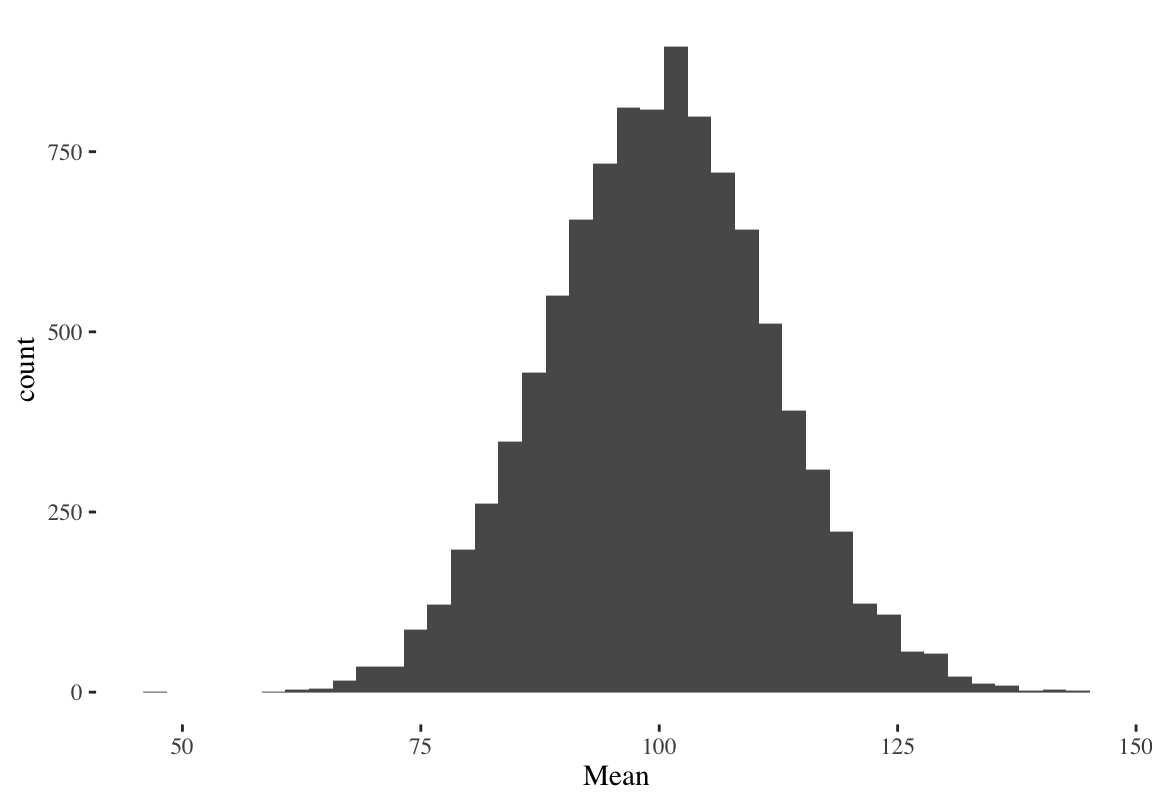
\includegraphics{08_inferential_files/figure-latex/jaotus-1.pdf}
\caption{\label{fig:jaotus}Keskmiste jaotus 10 000 valimist.}
\end{figure}

\begin{Shaded}
\begin{Highlighting}[]
\KeywordTok{mean}\NormalTok{(Summary}\OperatorTok{$}\NormalTok{Mean) }
\CommentTok{#> [1] 100}
\KeywordTok{mean}\NormalTok{(Summary}\OperatorTok{$}\NormalTok{SD)}
\CommentTok{#> [1] 17.8}
\end{Highlighting}
\end{Shaded}

Oh-hooo. Paljude valimite keskmiste keskmine ennustab väga täpselt
populatsiooni keskmist aga sd-de keskmise keskmine alahindab
populatsiooni sd-d. Valem, millega sd-d arvutatakse, töötab lihtsalt
kallutatult, kui n on väike (\textless{}10). Kes ei usu, kordab
simulatsiooni valimiga, mille N=30.

Ja nüüd 10 000 SD keskväärtused:



\begin{Shaded}
\begin{Highlighting}[]
\NormalTok{Summary }\OperatorTok\StringTok{ }
\StringTok{  }\KeywordTok{ggplot}\NormalTok{(}\KeywordTok{aes}\NormalTok{(SD)) }\OperatorTok{+}\StringTok{ }
\StringTok{  }\KeywordTok{geom_histogram}\NormalTok{(}\DataTypeTok{bins =} \DecValTok{40}\NormalTok{)}
\end{Highlighting}
\end{Shaded}

\begin{figure}
\centering
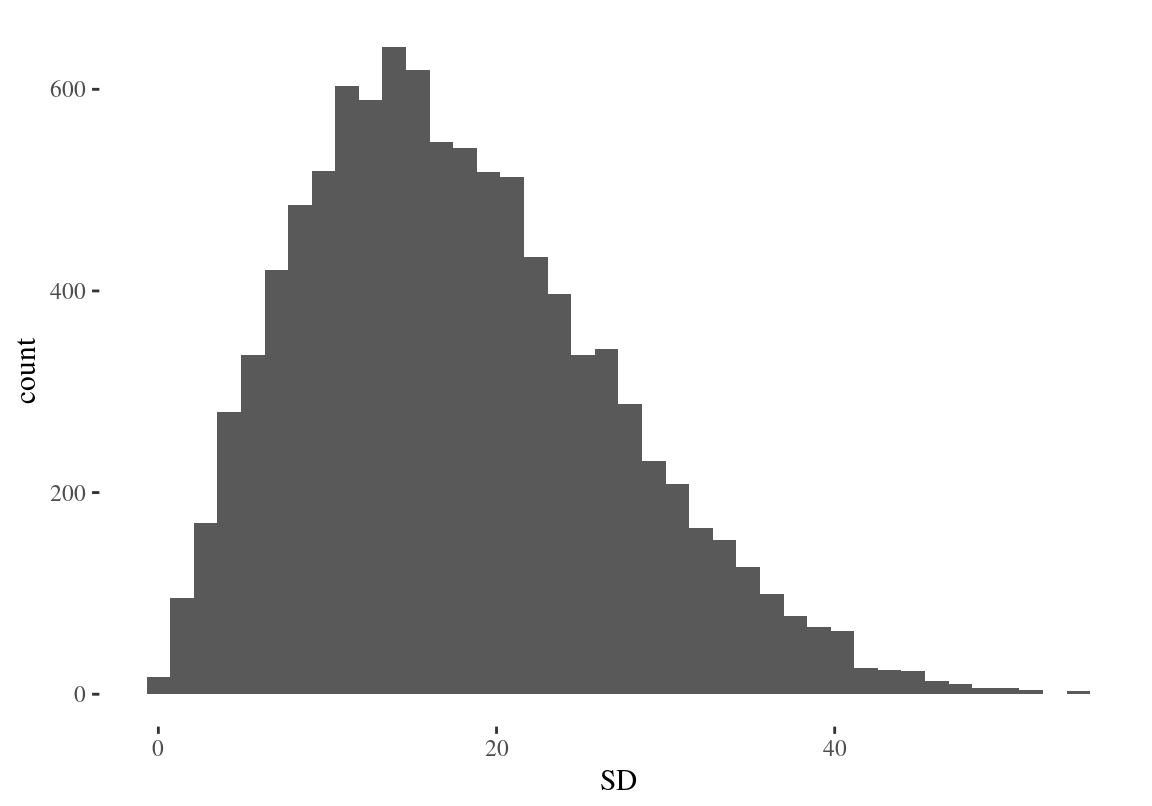
\includegraphics{08_inferential_files/figure-latex/sdjaotus-1.pdf}
\caption{\label{fig:sdjaotus}SD-de jaotus 10 000 valimist.}
\end{figure}

\begin{Shaded}
\begin{Highlighting}[]
\NormalTok{mode <-}\StringTok{ }\ControlFlowTok{function}\NormalTok{(x, }\DataTypeTok{adjust =} \DecValTok{1}\NormalTok{)\{}
\NormalTok{  x <-}\StringTok{ }\KeywordTok{na.omit}\NormalTok{(x)}
\NormalTok{  dx <-}\StringTok{ }\KeywordTok{density}\NormalTok{(x, }\DataTypeTok{adjust =}\NormalTok{ adjust)}
\NormalTok{  dx}\OperatorTok{$}\NormalTok{x[}\KeywordTok{which.max}\NormalTok{(dx}\OperatorTok{$}\NormalTok{y)]}
\NormalTok{\}}
\KeywordTok{mode}\NormalTok{(Summary}\OperatorTok{$}\NormalTok{SD) }
\CommentTok{#> [1] 14.1}
\end{Highlighting}
\end{Shaded}

SD-de jaotus on ebasümmeetriline ja mood ehk kõige tõenäolisem valimi sd
väärtus, mida võiksime oodata, on u 14, samal ajal kui populatsiooni sd
= 20. Lisaks alahinnatud keskmisele sd-le on sd-de jaotusel paks saba,
mis tagab, et teisest küljest pole ka vähetõenäoline, et meie valimi sd
populatsiooni sd-d kõvasti üle hindab.

Arvutame, mitu \% valimite sd-e keskmistest on \textgreater{} 25

\begin{Shaded}
\begin{Highlighting}[]
\KeywordTok{mean}\NormalTok{(Summary}\OperatorTok{$}\NormalTok{SD }\OperatorTok{>}\StringTok{ }\DecValTok{25}\NormalTok{)}
\CommentTok{#> [1] 0.211}
\end{Highlighting}
\end{Shaded}

Me saame \textgreater{}20\% tõenäosusega pahasti ülehinnatud SD.

\begin{Shaded}
\begin{Highlighting}[]
\KeywordTok{mean}\NormalTok{(Summary}\OperatorTok{$}\NormalTok{SD }\OperatorTok{<}\StringTok{ }\DecValTok{15}\NormalTok{)}
\CommentTok{#> [1] 0.434}
\end{Highlighting}
\end{Shaded}

Ja me saame \textgreater{}40\% tõenäosusega pahasti alahinnatud sd.
Selline on väikeste valimite traagika.

Aga vähemalt populatsiooni keskmise saame me palju valimeid tõmmates
ilusasti kätte --- ka väga väikeste valimitega.

Kahjuks pole meil ei vahendeid ega kannatust loodusest 10 000 valimi
kogumiseks. Enamasti on meil üksainus valim. Õnneks pole sellest väga
hullu, sest meil on olemas analoogne meetod, mis töötab üsna hästi ka
ühe valimiga. Me teeme lihtsalt ühest valimist mitu, mis meenutab pisut
mittemillegist midagi tegemist, aga veidi üllatuslikult töötab selles
kontekstis üsna hästi. Seda metoodikat kutsutakse
\emph{bootstrappimiseks} ja selle võttis esimesena kasutusele parun von
Münchausen. Too jutukas parun nimelt suutis end soomülkast iseenda patsi
pidi välja tõmmata (koos hobusega), mis ongi bootstrappimise põhimõte.
(Inglise kultuuriruumis tõmbab bootstrappija ennast mülkast välja oma
saapaserva pidi -- siit ka meetodi nimi.) Statistika tõmbas oma saapaid
pidi mülkast välja Brad Efron 1979. aastal.





\begin{figure}
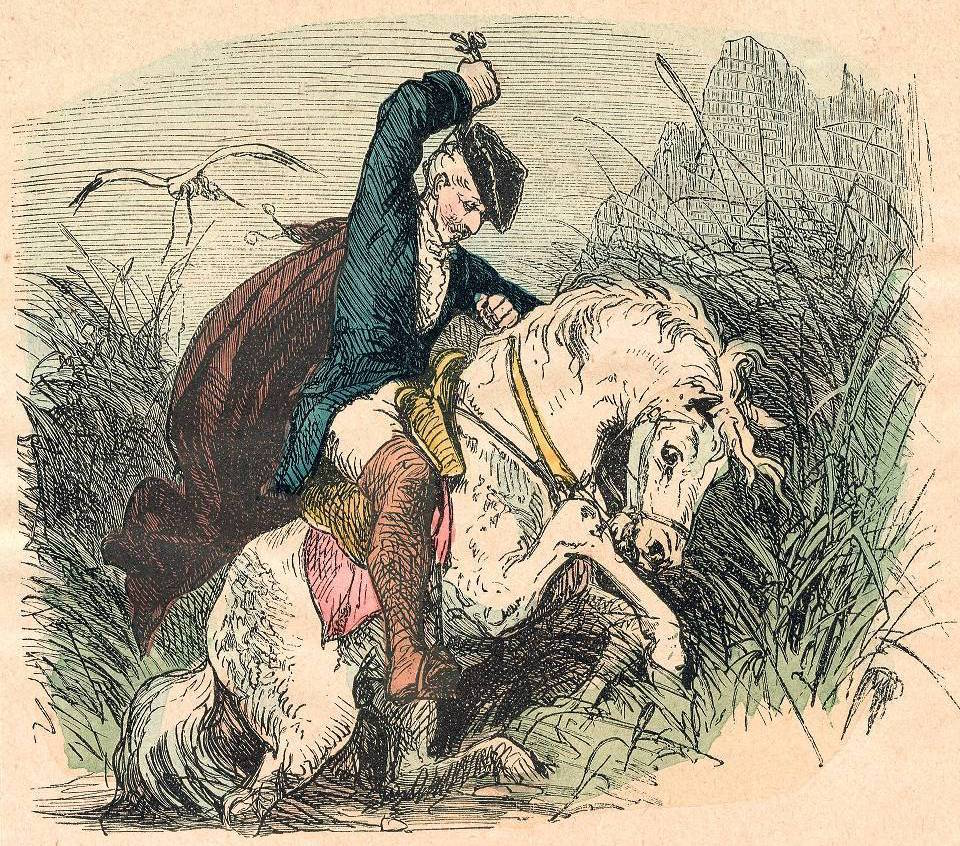
\includegraphics[width=0.5\linewidth]{img/munchausen} \caption{Nii nagu parun Münchausen tõmbas ennast patsi pidi mülkast
välja, genereeritakse bootstrappimisega algse valimi põhjal
teststatistiku jaotus.}\label{fig:parun}
\end{figure}

\part{OSA}\label{part-osa-1}

\chapter{Bootstrap}\label{bootstrap}

\begin{Shaded}
\begin{Highlighting}[]
\KeywordTok{library}\NormalTok{(rethinking)}
\KeywordTok{library}\NormalTok{(bayesboot)}
\KeywordTok{library}\NormalTok{(dplyr)}
\KeywordTok{library}\NormalTok{(purrr)}
\KeywordTok{library}\NormalTok{(ggplot2)}
\KeywordTok{library}\NormalTok{(modelr)}
\end{Highlighting}
\end{Shaded}

\begin{quote}
Populatsioon on valimile sama, mis on valim bootstrappitud valimile.
\end{quote}

Nüüd alustame ühestainsast empiirilisest valimist ja genereerime sellest
2000 virtuaalset valimit. Selleks tõmbame me oma valimist virtuaalselt
2000 uut juhuvalimit (bootstrap valimit), millest igaüks on sama suur
kui algne valim. Saladus seisneb selles, et bootstrap valimite tõmbamine
käib asendusega, st iga empiirilise valimi element, mis bootstrap
valimisse tõmmatakse, pannakse kohe algsesse valimisse tagasi. Seega
saab seda elementi kohe uuesti samasse bootstrap valimisse tõmmata (kui
juhus nii tahab). Seega sisaldab tüüpiline bootstrap valim osasid algse
valimi numbreid mitmes korduses ja teisi üldse mitte. Iga bootstrap
valimi põhjal arvutatakse meid huvitav statistik (näiteks keskväärtus)
ja kõik need 2000 bootstrapitud statistikut plotitakse samamoodi, nagu
me ennist tegime valimitega lõpmata suurest populatsioonist. Ainsad
erinevused on, et bootstrapis võrdub andmekogu suurus, millest bootstrap
valimeid tõmmatakse, algse valimi suurusega ning, et iga bootstrapi
valim on sama suur kui algne valim (sest meie poolt arvutatud statistiku
varieeruvus, me tahame oma bootstrap valimiga tabada, sõltub valimi
suurusest). Tüüpiliselt kasutatakse bootstrapitud statistikuid selleks,
et arvutada usaldusintervall statistiku väärtusele.

\begin{quote}
Bootstrap ei muuda meie hinnangut statistiku punktväärtusele. Ta annab
hinnangu ebakindluse määrale, mida me oma valimi põhjal peaksime tundma
selle punkthinnangu kohta.
\end{quote}

Bootstrappimine on üldiselt väga hea meetod, mis sõltub väiksemast
arvust eeldustest kui statistikas tavaks. Bootstrap ei eelda, et andmed
on normaaljaotusega või mõne muu matemaatiliselt lihtsa jaotusega. Tema
põhiline eeldus on, et valim peegeldab populatsiooni -- mis ei pruugi
kehtida väikeste valimite korral ja kallutatud (mitte-juhuslike)
valimite korral. Lisaks, tavaline bootstrap ei sobi hierarhiliste
andmestruktuuride analüüsiks ega näiteks aegridade analüüsiks.
Bootstrappida saab edukalt enamusi statistikuid, mida te võiksite elu
jooksul arvutada, aga on siiski erandeid: näiteks valimi maksimum ja
miinimumväärtused.

Bootstrap empiirilisele valimile suurusega n töötab nii:

\begin{enumerate}
\def\labelenumi{\arabic{enumi}.}
\tightlist
\item
  tõmba (asendusega) empiirilisest valimist B uut virtuaalset valimit (B
  bootstrap valimit), igaüks suurusega n.
\item
  arvuta keskmine, sd või mistahes muu statistik igale bootstrapi
  valimile. Tee seda B korda.
\item
  joonista oma statistiku väärtustest histogramm või density plot
\end{enumerate}

Nende andmete põhjal saab küsida palju toreidaid küsimusi --- vt
allpool.

Mis on USA presidentide keskmine pikkus? Meil on viimase 11 presidendi
pikkused.










\begin{Shaded}
\begin{Highlighting}[]
\NormalTok{heights <-}\StringTok{ }\KeywordTok{tibble}\NormalTok{(}\DataTypeTok{value =} \KeywordTok{c}\NormalTok{(}\DecValTok{183}\NormalTok{, }\DecValTok{192}\NormalTok{, }\DecValTok{182}\NormalTok{, }\DecValTok{183}\NormalTok{, }\DecValTok{177}\NormalTok{, }\DecValTok{185}\NormalTok{, }\DecValTok{188}\NormalTok{, }\DecValTok{188}\NormalTok{, }\DecValTok{182}\NormalTok{, }\DecValTok{185}\NormalTok{, }\DecValTok{188}\NormalTok{))}
\NormalTok{B <-}\StringTok{ }\DecValTok{1000} \CommentTok{# the number of bootstrap samples}

\NormalTok{mean_value <-}\StringTok{ }\ControlFlowTok{function}\NormalTok{(x) }\KeywordTok{mean}\NormalTok{(}\KeywordTok{as.data.frame}\NormalTok{(x)}\OperatorTok{$}\NormalTok{value, }\DataTypeTok{na.rm =} \OtherTok{TRUE}\NormalTok{) }\CommentTok{# helper function}
\NormalTok{boot <-}\StringTok{ }\KeywordTok{bootstrap}\NormalTok{(heights, B)}
\NormalTok{boot <-}\StringTok{ }\NormalTok{boot }\OperatorTok\StringTok{ }
\StringTok{            }\KeywordTok{mutate}\NormalTok{(}\DataTypeTok{Mean =} \KeywordTok{map_dbl}\NormalTok{(strap, mean_value))}

\KeywordTok{ggplot}\NormalTok{(boot, }\KeywordTok{aes}\NormalTok{(Mean)) }\OperatorTok{+}\StringTok{ }\KeywordTok{geom_density}\NormalTok{()}
\end{Highlighting}
\end{Shaded}

\begin{figure}
\centering
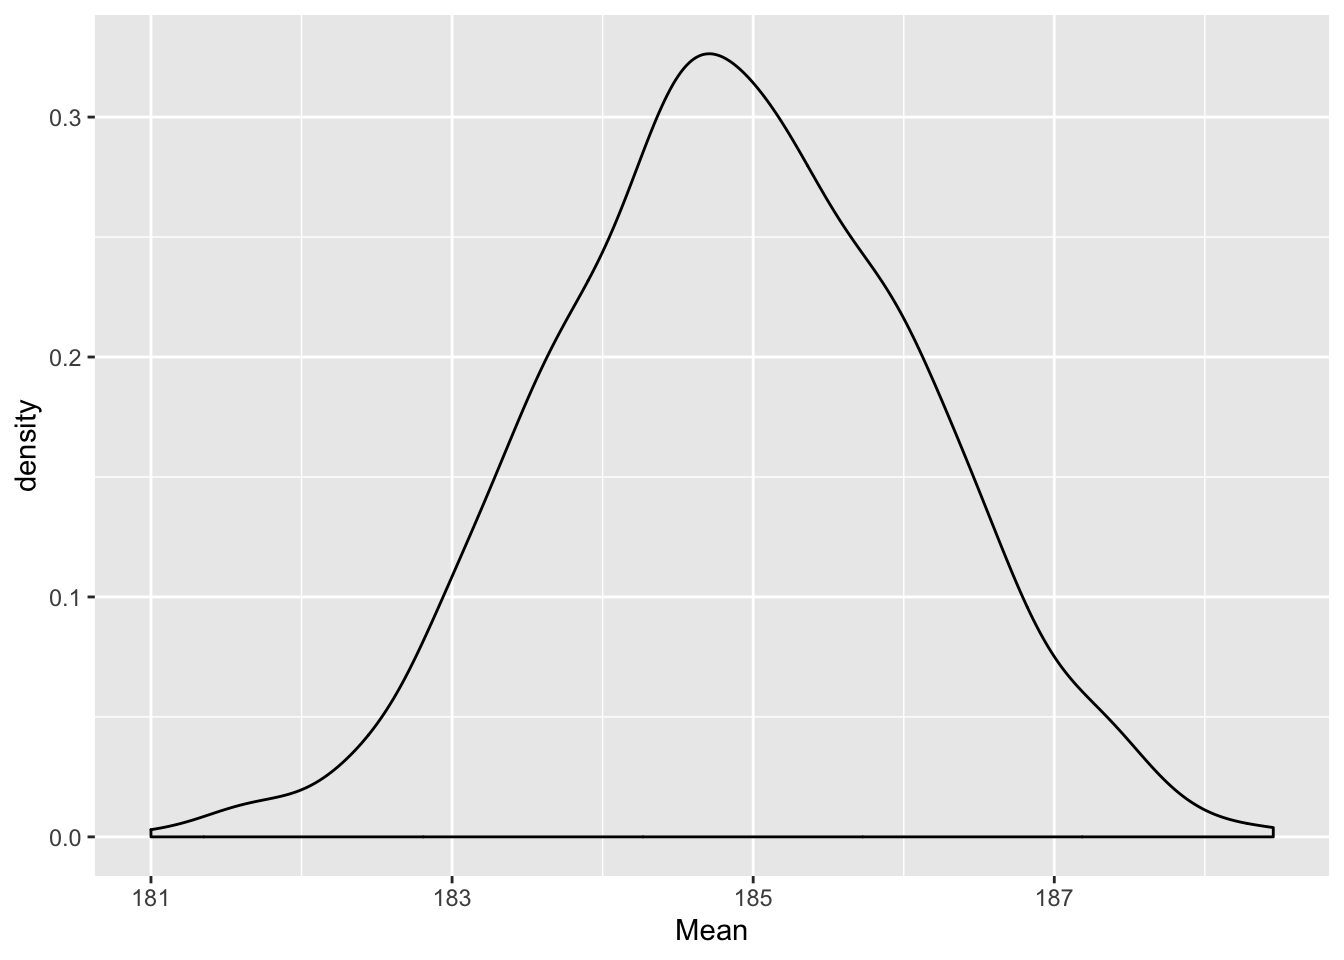
\includegraphics{09_bootstrap_files/figure-latex/bootpost-1.pdf}
\caption{\label{fig:bootpost}Bootstrapitud posteerior USA presidentide keskmisele
pikkusele. Järgnevas koodis ütleme me kõigepealt, et B = 2000 (et me
võtame 2000 bootstrap valimit) kasutades selleks broom paketi käsku
boot(), millele on lihtne lisada dplyri funktsioon summarise(). Siiski
peame seda tegema dplyr::do() abil. Pane tähele, et ``tänu'' do()
kasutamisele peame me summarise() funktsioonis näitama punktiga koha,
kuhu lähevad \%\textgreater{}\% torust tulnud bootstrap valimid. Aga
muidu on kõik tavapärane tidyverse.}
\end{figure}

ehk sama asi ilma bootsrtap functsiooni kasutamata.

\begin{Shaded}
\begin{Highlighting}[]
\NormalTok{heights <-}\StringTok{ }\KeywordTok{tibble}\NormalTok{(}\DataTypeTok{value =} \KeywordTok{c}\NormalTok{(}\DecValTok{183}\NormalTok{, }\DecValTok{192}\NormalTok{, }\DecValTok{182}\NormalTok{, }\DecValTok{183}\NormalTok{, }\DecValTok{177}\NormalTok{, }\DecValTok{185}\NormalTok{, }\DecValTok{188}\NormalTok{, }\DecValTok{188}\NormalTok{, }\DecValTok{182}\NormalTok{, }\DecValTok{185}\NormalTok{, }\DecValTok{188}\NormalTok{))}
\NormalTok{n <-}\StringTok{ }\KeywordTok{nrow}\NormalTok{(heights) }\CommentTok{#empirical sample size}
\NormalTok{B <-}\StringTok{ }\DecValTok{1000} \CommentTok{#nr of bootstrap samples}
\NormalTok{boot1 <-}\StringTok{  }\KeywordTok{replicate}\NormalTok{(B, }\KeywordTok{sample_n}\NormalTok{(heights, n, }\DataTypeTok{replace =} \OtherTok{TRUE}\NormalTok{)) }

\NormalTok{df22 <-}\StringTok{ }\NormalTok{boot1 }\OperatorTok\StringTok{ }\CommentTok{#boot1 object is a list}
\StringTok{  }\KeywordTok{as.data.frame}\NormalTok{() }\OperatorTok\StringTok{ }\CommentTok{#convert this list into a data frame }
\StringTok{  }\KeywordTok{summarise_all}\NormalTok{(mean) }\OperatorTok\StringTok{ }\KeywordTok{t}\NormalTok{() }\OperatorTok\StringTok{ }\KeywordTok{as_tibble}\NormalTok{() }

\KeywordTok{ggplot}\NormalTok{(df22, }\KeywordTok{aes}\NormalTok{(V1)) }\OperatorTok{+}\StringTok{ }\KeywordTok{geom_histogram}\NormalTok{()}
\end{Highlighting}
\end{Shaded}

Mida selline keskväärtuste jaotus tähendab? Me võime seda vaadelda
posterioorse tõenäosusjaotusena. Selle tõlgenduse kohaselt iseloomustab
see jaotus täpselt meie usku presidentide keskmise pikkuse kohta,
niipalju kui see usk põhineb bootstrappimises kasutatud andmetel.
Senikaua, kui meil pole muud relevantset teavet, on kõik, mida me usume
teadvat USA presidentide keskmise pikkuse kohta, peidus selles jaotuses.
Need pikkused, mille kohal jaotus on kõrgem, sisaldavad meie jaoks
tõenäolisemalt tegelikku USA presidentide keskmist pikkust kui need
pikkused, mille kohal posterioorne jaotus on madalam.

Kuidas selle jaotusega edasi töötada? See on lihtne: meil on 2000 arvu
(2000 bootstrapitud statistiku väärtust) ja me teeme nendega kõike seda,
mida parasjagu tahame.

Näiteks me võime arvutada, millisesse pikkuste vahemikku jääb 92\% meie
usust USA presidentide tõelise keskmise pikkuse kohta. See tähendab, et
teades seda vahemikku peaksime olema valmis maksma mitte rohkem kui 92
senti pileti eest, mis juhul kui USA presidentide keskmine pikkus tõesti
jääb sinna vahemikku, toob meile võidu suuruses 1 EUR (ja 8 senti
kasumit). Selline kihlveokontor on täiesti respektaabel ja akadeemiline
tõenäosuse tõlgendus; see on paljude arvates lausa parim tõlgendus, mis
meil on.

Miks just 92\% usaldusinterval? Vastus on, et miks mitte? Meil pole
ühtegi universaalset põhjust eelistada üht usaldusvahemiku suurust
teisele. Olgu meil usaldusinteval 90\%, 92\% või 95\% --- tõlgendus on
ikka sama. Nimelt, et me usume, et suure tõenäosusega jääb tegelik
keskväärtus meie poolt arvutatud vahemikku. Mudeli ja maailma erinevused
tingivad niikuinii selle, et konkreetne number ei kandu mudelist otse
üle pärismaailma. Eelnevalt mainitud kihlveokontor töötab mudeli
maailmas, mitte teie kodulähedasel hipodroomil.

92\% usaldusintervalli arvutamiseks on kaks meetodit, mis enamasti
annavad vaid veidi erinevaid tulemusi.

\begin{enumerate}
\def\labelenumi{\arabic{enumi}.}
\tightlist
\item
  HPDI --- Highest Density Probability Interval --- alustab jaotuse
  tipust (tippudest) ja katab 92\% jaotuse kõrgema(te) osa(de) pindalast
\end{enumerate}

\begin{Shaded}
\begin{Highlighting}[]
\KeywordTok{HPDI}\NormalTok{(heights}\OperatorTok{$}\NormalTok{value, }\DataTypeTok{prob =} \FloatTok{0.92}\NormalTok{)}
\CommentTok{#> |0.92 0.92| }
\CommentTok{#>   177   192}
\end{Highlighting}
\end{Shaded}

\begin{enumerate}
\def\labelenumi{\arabic{enumi}.}
\setcounter{enumi}{1}
\tightlist
\item
  PI --- Probability Interval --- alustab jaotuse servadest ja katab
  kummagist servast 4\% jaotuse pindalast. PI 90\%-le on sama, mis
  arvutada 5\% ja 95\% kvantiilid (jne).
\end{enumerate}

\begin{Shaded}
\begin{Highlighting}[]
\KeywordTok{PI}\NormalTok{(heights}\OperatorTok{$}\NormalTok{value, }\DataTypeTok{prob =} \FloatTok{0.90}\NormalTok{)}
\CommentTok{#>  5% 95% }
\CommentTok{#> 180 190}
\CommentTok{# quantile(heights$value, probs = c(0.05, 0.95)) teeb sama asja}
\end{Highlighting}
\end{Shaded}

HPDI on üldiselt parem mõõdik kui PI, aga teatud juhtudel on seda raskem
arvutada. Kui HPDI ja PI tugevalt erinevad, on hea mõte piirduda jaotuse
enda avaldamisega --- jaotus ise sisaldab kogu informatsiooni, mis meil
on oma statistiku väärtuse kohta. Intervallid on lihtsalt summaarsed
statistikud andmete kokkuvõtlikuks esitamiseks.

Kui suure tõenäosusega on USA presidentide keskmine pikkus suurem kui
USA populatsiooni meeste keskmine pikkus (178.3 cm mediaan)?

\begin{Shaded}
\begin{Highlighting}[]
\KeywordTok{mean}\NormalTok{(heights}\OperatorTok{$}\NormalTok{value }\OperatorTok{>}\StringTok{ }\FloatTok{178.3}\NormalTok{)}
\CommentTok{#> [1] 0.909}
\end{Highlighting}
\end{Shaded}

Ligikaudu 100\% tõenäosusega (valimis on 1 mees alla 182 cm, ja tema on
177 cm). Lühikesed jupatsid ei saa Ameerikamaal presidendiks!

\textbf{Kuidas lahendada bootstrap, kui mei tahame usaldusintervalle
kahe ebavõrdse grupi erinevusele?} Näiteks kui meil on katsegrupis N =
25 ja kontrollgrupis N = 20, ja me tahame arvutada statistikut ES =
katsegrupi keskmine - kontrollgrupi keskmine.

\begin{enumerate}
\def\labelenumi{\arabic{enumi}.}
\item
  tõbma katsegrupist N = 25 bootstrapvalim
\item
  tõmba kontrollgrupist N = 20 bootsrapvalim
\item
  lahuta kontrollgrupi bootstrapvalimi mediaan katsegrupi omast (või
  aritmeetriline keskmine või ükskõik mis muu keskmise näitaja, mida
  hing ihaldab)
\item
  korda punkte 1-3 B korda ja tööta edasi bootstrapjaptusega, nagu
  eespool näidatud.
\end{enumerate}

\section{Mõned tava-bootstrapi
paketid}\label{moned-tava-bootstrapi-paketid}

Professionaalid kasutavad boot paketti, mis on suhteliselt ebameeldiva
süntaksiga, aga väga laialt rakendatav. Boot paketi peale on ehitatud
tavainimesele hästi kasutatav pakett bootES (Kirby and Gelranc, 2013,
Behav Res 45:905--927), mis teeb lihtsaks usalduspiiride leidmise
erinevat tüüpi efekti suurustele, kaasa arvatud lihtsad hierarhilised ja
ühefaktorilise ANOVA tüüpi katseskeemid. Nendes pakettides tasub
üldjuhul kasutada meetodit nimega BCa (bias-corrected-and-accelerated)
usalduspiiride arvutamiseks. See meetod püüab parandada
bootstrap-valimite võimalikku kallutatust (esineb sedavõrd, kui
bootstrap-jaotuse tipp ei ole samas kohas kui oleks paljude
päris-valimite pealt arvutatud statistikute jaotuse tipp) ja olukorda,
kus statistiku väärtuse varieeruvuse määr sõltub statistiku väärtusest.
BCa edukaks arvutamiseks peab bootstrap valimite arv tuntavalt ületama
valimi suurust. Simulatsioonidega on näidatud, et BCa (ja teisi)
usalduspiire saab mõistlikult arvutada valimitelt, mille suurus on
\textgreater{} 15. Sellest väiksemate valimite korral peate eeldama, et
teie usaldusinetvallid valetavad. Aegridade, kus esineb järjestikuste
ajapunktide vahelisi sõltuvusi, tuleks kasutada nn block bootstrappi,
mida implementerrib näiteks boot::tsboot().

\section*{Bayesi bootstrap}\label{bayesi-bootstrap}
\addcontentsline{toc}{section}{Bayesi bootstrap}

Kui klassikalise bootstrap meetodi pakkus välja B. Efron aastal 1979,
siis selle Bayesi versioon avaldati D.B. Rubini poolt 1981. a. Bayesi
versioon bootstrapist on implementeeritud ``bayesboot'' paketis
funktsioonis \texttt{bayesboot()}. Hea lihtsa seletuse Bayesi bootstrapi
kohta saab siit \url{https://www.youtube.com/watch?v=WMAgzr99PKE} ja
lihtsa r koodi selle meetodi rakendamiseks saab siit
\url{https://www.r-bloggers.com/simple-bayesian-bootstrap/}.

Lühidalt, erinevalt eelkirjeldatud tava-bootstrapist simuleeritakse
Bayesi bootstrapis posterioorjaotused, näiteks arvutatakse kaalutud
keskmine, kus ühtlasest jaotusest pärit kaalud on prioriks.

Näited sellest, kuidas kasutada bayesbooti standardhälbe,
korrelatsioonikoefitsiendi ja lineaarse mudeli koefitsientide
usalduspiiride arvutamiseks leiate \texttt{?bayesboot} käsuga.




\begin{Shaded}
\begin{Highlighting}[]
\NormalTok{heights_bb <-}\StringTok{ }\KeywordTok{bayesboot}\NormalTok{(heights}\OperatorTok{$}\NormalTok{value, mean)}
\KeywordTok{plot}\NormalTok{(heights_bb, }\DataTypeTok{compVal =} \DecValTok{185}\NormalTok{)}
\end{Highlighting}
\end{Shaded}

\begin{figure}
\centering
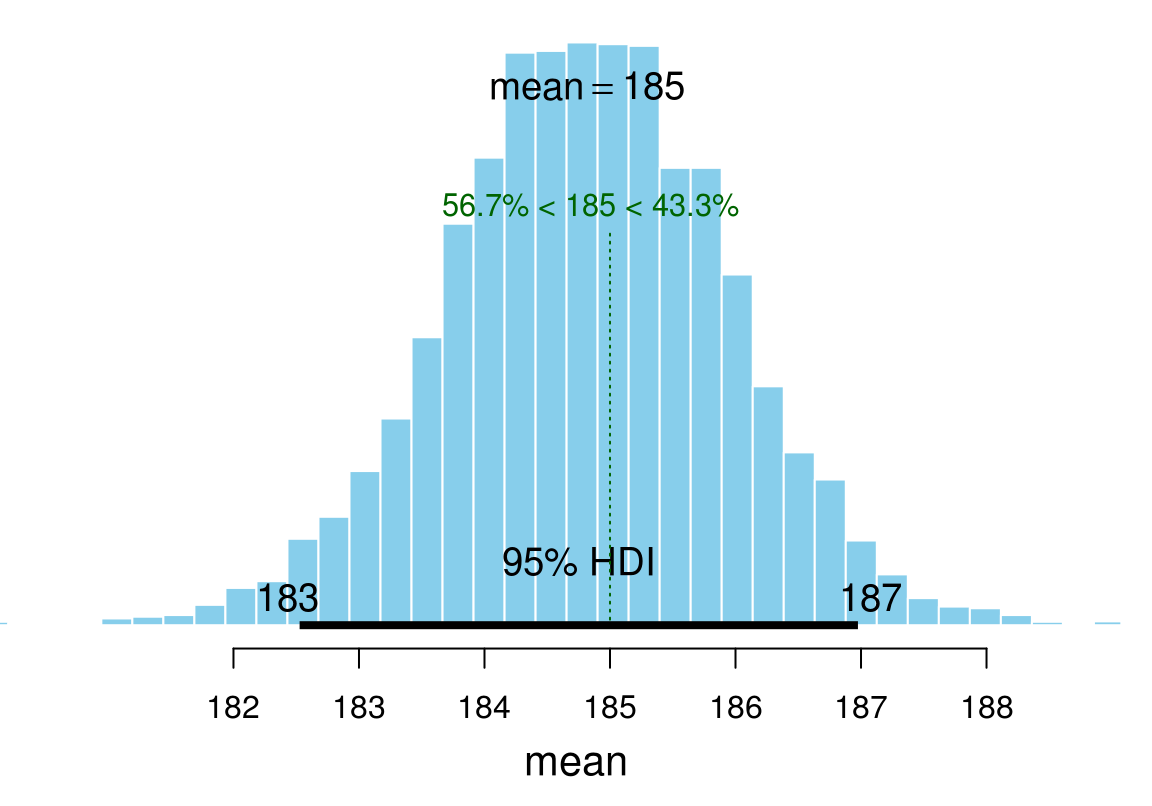
\includegraphics{09_bootstrap_files/figure-latex/bayesboot-1.pdf}
\caption{\label{fig:bayesboot}Bayesi bootstrapi posteerior USA presidentide keskmisele
pikkusele.}
\end{figure}

\begin{Shaded}
\begin{Highlighting}[]
\KeywordTok{HPDI}\NormalTok{(heights_bb}\OperatorTok{$}\NormalTok{V1, }\DataTypeTok{prob =} \FloatTok{0.95}\NormalTok{)}
\CommentTok{#> |0.95 0.95| }
\CommentTok{#>   183   187}
\end{Highlighting}
\end{Shaded}

Vaikimisi pannakse \texttt{bayesboot()} funktsioonis statistiku
arvutamisel kaalud (prior) valimi indeksile, mis annab erineva tulemuse
kui näiteks kaalutud keskmise arvutamisel, kus kaalud (prior) pannakse
valimi väärtustele.

Aritmeetilise keskmise Bayesi bootstrap väärtused kasutades kaalutud
keskmise funktsiooni \texttt{weighted.mean} saab niimoodi:

\begin{Shaded}
\begin{Highlighting}[]
\NormalTok{heights_bb_w <-}\StringTok{ }\KeywordTok{bayesboot}\NormalTok{(heights}\OperatorTok{$}\NormalTok{value, }
\NormalTok{                         weighted.mean, }
                         \DataTypeTok{use.weights =} \OtherTok{TRUE}\NormalTok{)}
\end{Highlighting}
\end{Shaded}

Tõenäosus, et keskmine on suurem kui 182 cm

\begin{Shaded}
\begin{Highlighting}[]
\KeywordTok{mean}\NormalTok{(heights_bb[, }\DecValTok{1}\NormalTok{] }\OperatorTok{>}\StringTok{ }\DecValTok{182}\NormalTok{)}
\CommentTok{#> [1] 0.993}
\end{Highlighting}
\end{Shaded}

Kahe keskväärtuse erinevus (ES = keskmine1 - keskmine2):



\begin{Shaded}
\begin{Highlighting}[]
\KeywordTok{set.seed}\NormalTok{(}\DecValTok{1}\NormalTok{)}
\NormalTok{## Simulate two random normal distributions with mean 0. }
\NormalTok{## True difference is 0.}
\NormalTok{dfr <-}\StringTok{ }\KeywordTok{tibble}\NormalTok{(}\DataTypeTok{a =} \KeywordTok{rnorm}\NormalTok{(}\DecValTok{10}\NormalTok{, }\DecValTok{0}\NormalTok{, }\DecValTok{1}\NormalTok{), }
              \DataTypeTok{b =} \KeywordTok{rnorm}\NormalTok{(}\DecValTok{10}\NormalTok{, }\DecValTok{0}\NormalTok{, }\DecValTok{1}\NormalTok{),}
              \DataTypeTok{c =}\NormalTok{ a }\OperatorTok{-}\StringTok{ }\NormalTok{b)}
\NormalTok{dfr_bb <-}\StringTok{ }\KeywordTok{bayesboot}\NormalTok{(dfr}\OperatorTok{$}\NormalTok{c, weighted.mean, }\DataTypeTok{use.weights =} \OtherTok{TRUE}\NormalTok{ )}
\KeywordTok{plot}\NormalTok{(dfr_bb, }\DataTypeTok{compVal =} \DecValTok{0}\NormalTok{)}
\end{Highlighting}
\end{Shaded}

\begin{figure}
\centering
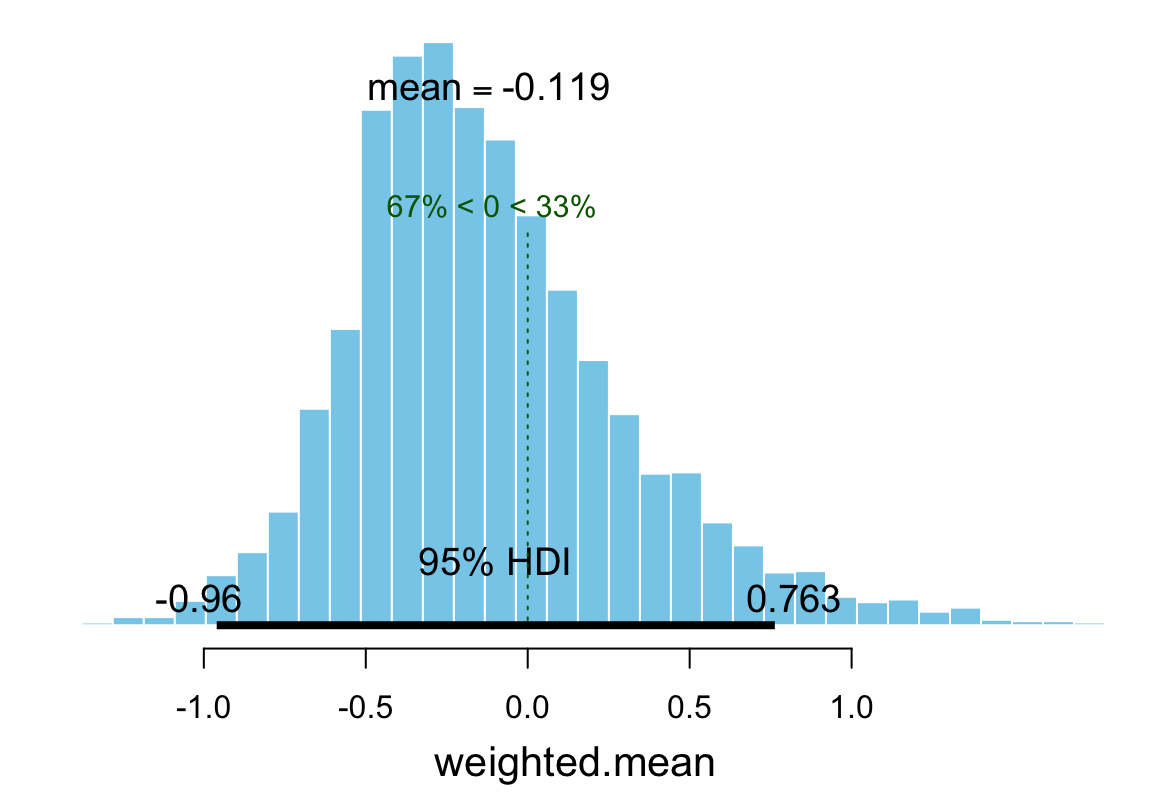
\includegraphics{09_bootstrap_files/figure-latex/bayeses-1.pdf}
\caption{\label{fig:bayeses}Bayesi bootstrap ES-le.}
\end{figure}

BayesianFirstAid raamatukogu funktsioon bayes.t.test() annab kasutades
t-jaotuse tõepäramudelit üsna täpselt sama vastuse. See raamatukogu
eeldab JAGS mcmc sämpleri installeerimist. Abi saab siit
\url{https://github.com/rasmusab/bayesian_first_aid} ja siit
\url{https://faculty.washington.edu/jmiyamot/p548/installing.jags.pdf}.

\section*{Parameetriline bootstrap}\label{parameetriline-bootstrap}
\addcontentsline{toc}{section}{Parameetriline bootstrap}

Kui me arvame, et me teame, mis jaotusega on meie andmed, ja meil on
suhteliselt vähe andmepunkte, võib olla mõistlik lisada bootstrapile
andmete jaotuse mudel. Näiteks, meie USA presidentide pikkused võiksid
olla umbkaudu normaaljaotusega (sest me teame, et USA meeste pikkused on
seda). Seega fitime kõigepealt presidentide pikkusandmetega
normaaljaotuse ja seejärel tõmbame bootsrap valimid sellest
normaaljaotuse mudelist. Normaaljaotuse mudelil on 2 parameetrit:
keskmine (mu) ja standardhälve (sigma), mida saame fittida valimiandmete
põhjal:




\begin{Shaded}
\begin{Highlighting}[]
\NormalTok{mu <-}\StringTok{ }\KeywordTok{mean}\NormalTok{(heights}\OperatorTok{$}\NormalTok{value)}
\NormalTok{sigma <-}\StringTok{ }\KeywordTok{sd}\NormalTok{(heights}\OperatorTok{$}\NormalTok{value)}
\NormalTok{N <-}\StringTok{ }\KeywordTok{length}\NormalTok{(heights}\OperatorTok{$}\NormalTok{value)}
\NormalTok{sample_means <-}\StringTok{ }\KeywordTok{tibble}\NormalTok{(}\DataTypeTok{value =} \KeywordTok{rnorm}\NormalTok{(N }\OperatorTok{*}\StringTok{ }\DecValTok{1000}\NormalTok{, mu, sigma), }
                       \DataTypeTok{indeks =} \KeywordTok{rep}\NormalTok{(}\DecValTok{1}\OperatorTok{:}\DecValTok{1000}\NormalTok{, }\DataTypeTok{each =}\NormalTok{ N))}

\NormalTok{sample_means_sum <-}\StringTok{ }\NormalTok{sample_means }\OperatorTok\StringTok{ }
\StringTok{  }\KeywordTok{group_by}\NormalTok{(indeks) }\OperatorTok\StringTok{ }
\StringTok{  }\KeywordTok{summarise}\NormalTok{(}\DataTypeTok{Mean =} \KeywordTok{mean}\NormalTok{(value))}

\KeywordTok{ggplot}\NormalTok{(sample_means_sum, }\KeywordTok{aes}\NormalTok{(}\DataTypeTok{x =}\NormalTok{ Mean)) }\OperatorTok{+}
\StringTok{  }\KeywordTok{geom_histogram}\NormalTok{(}\DataTypeTok{color =} \StringTok{"white"}\NormalTok{, }\DataTypeTok{bins =} \DecValTok{20}\NormalTok{)}
\end{Highlighting}
\end{Shaded}

\begin{figure}
\centering
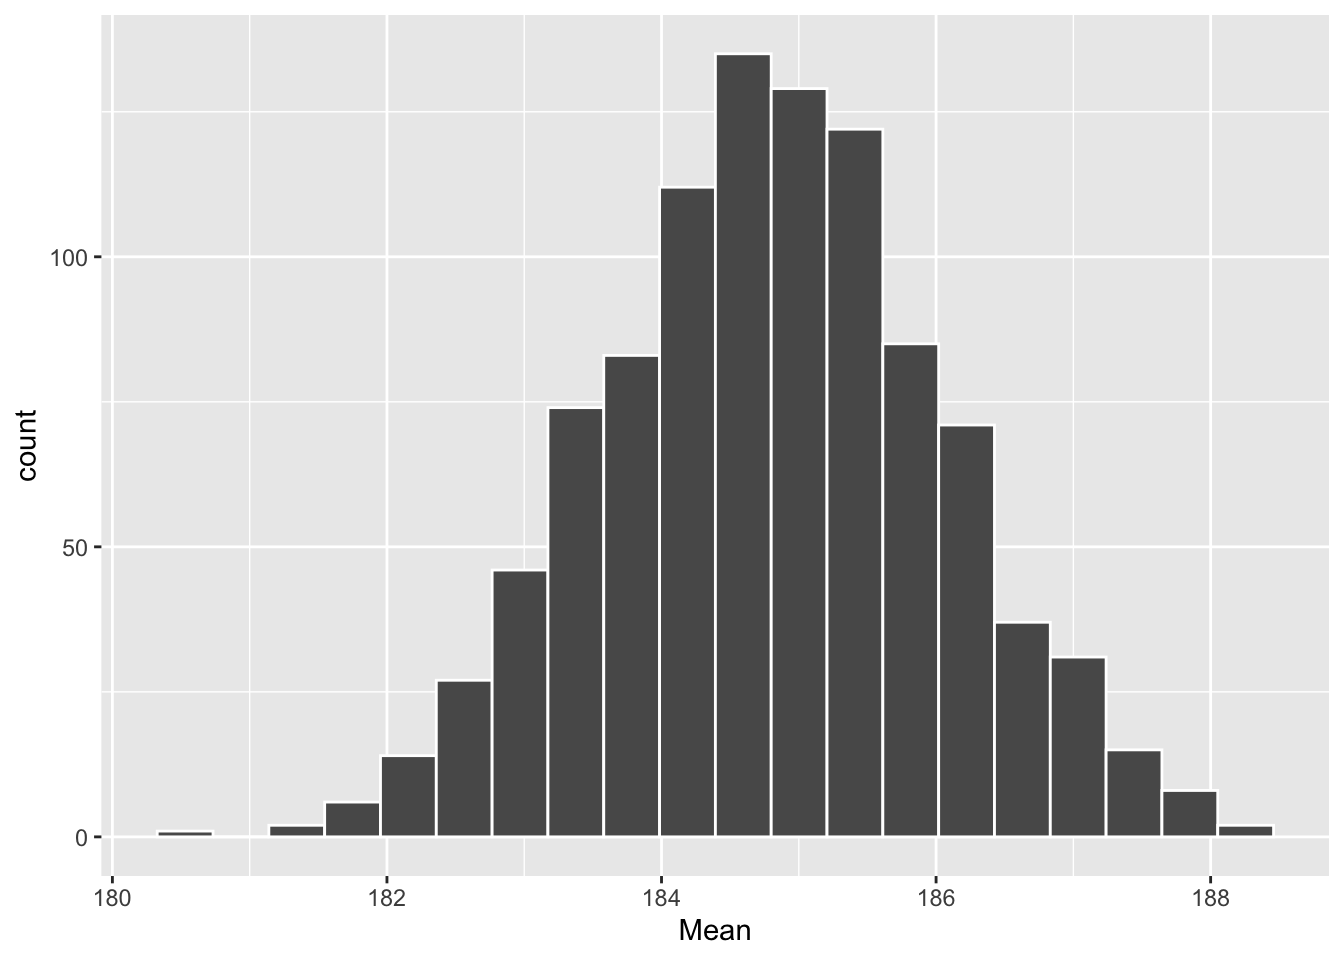
\includegraphics{09_bootstrap_files/figure-latex/paramboot-1.pdf}
\caption{\label{fig:paramboot}Parameetrilise bootstrapi posteerior USA presidentide
keskmisele pikkusele.}
\end{figure}

\begin{Shaded}
\begin{Highlighting}[]
\KeywordTok{HPDI}\NormalTok{(sample_means_sum}\OperatorTok{$}\NormalTok{Mean)}
\CommentTok{#> |0.89 0.89| }
\CommentTok{#>   183   187}
\end{Highlighting}
\end{Shaded}

Üldiselt ei soovita me parameetrilist bootstrappi väga soojalt, sest
täisbayesiaanlik alternatiiv, mida me kohe õppima asume, on sellest
paindlikum.



\begin{figure}
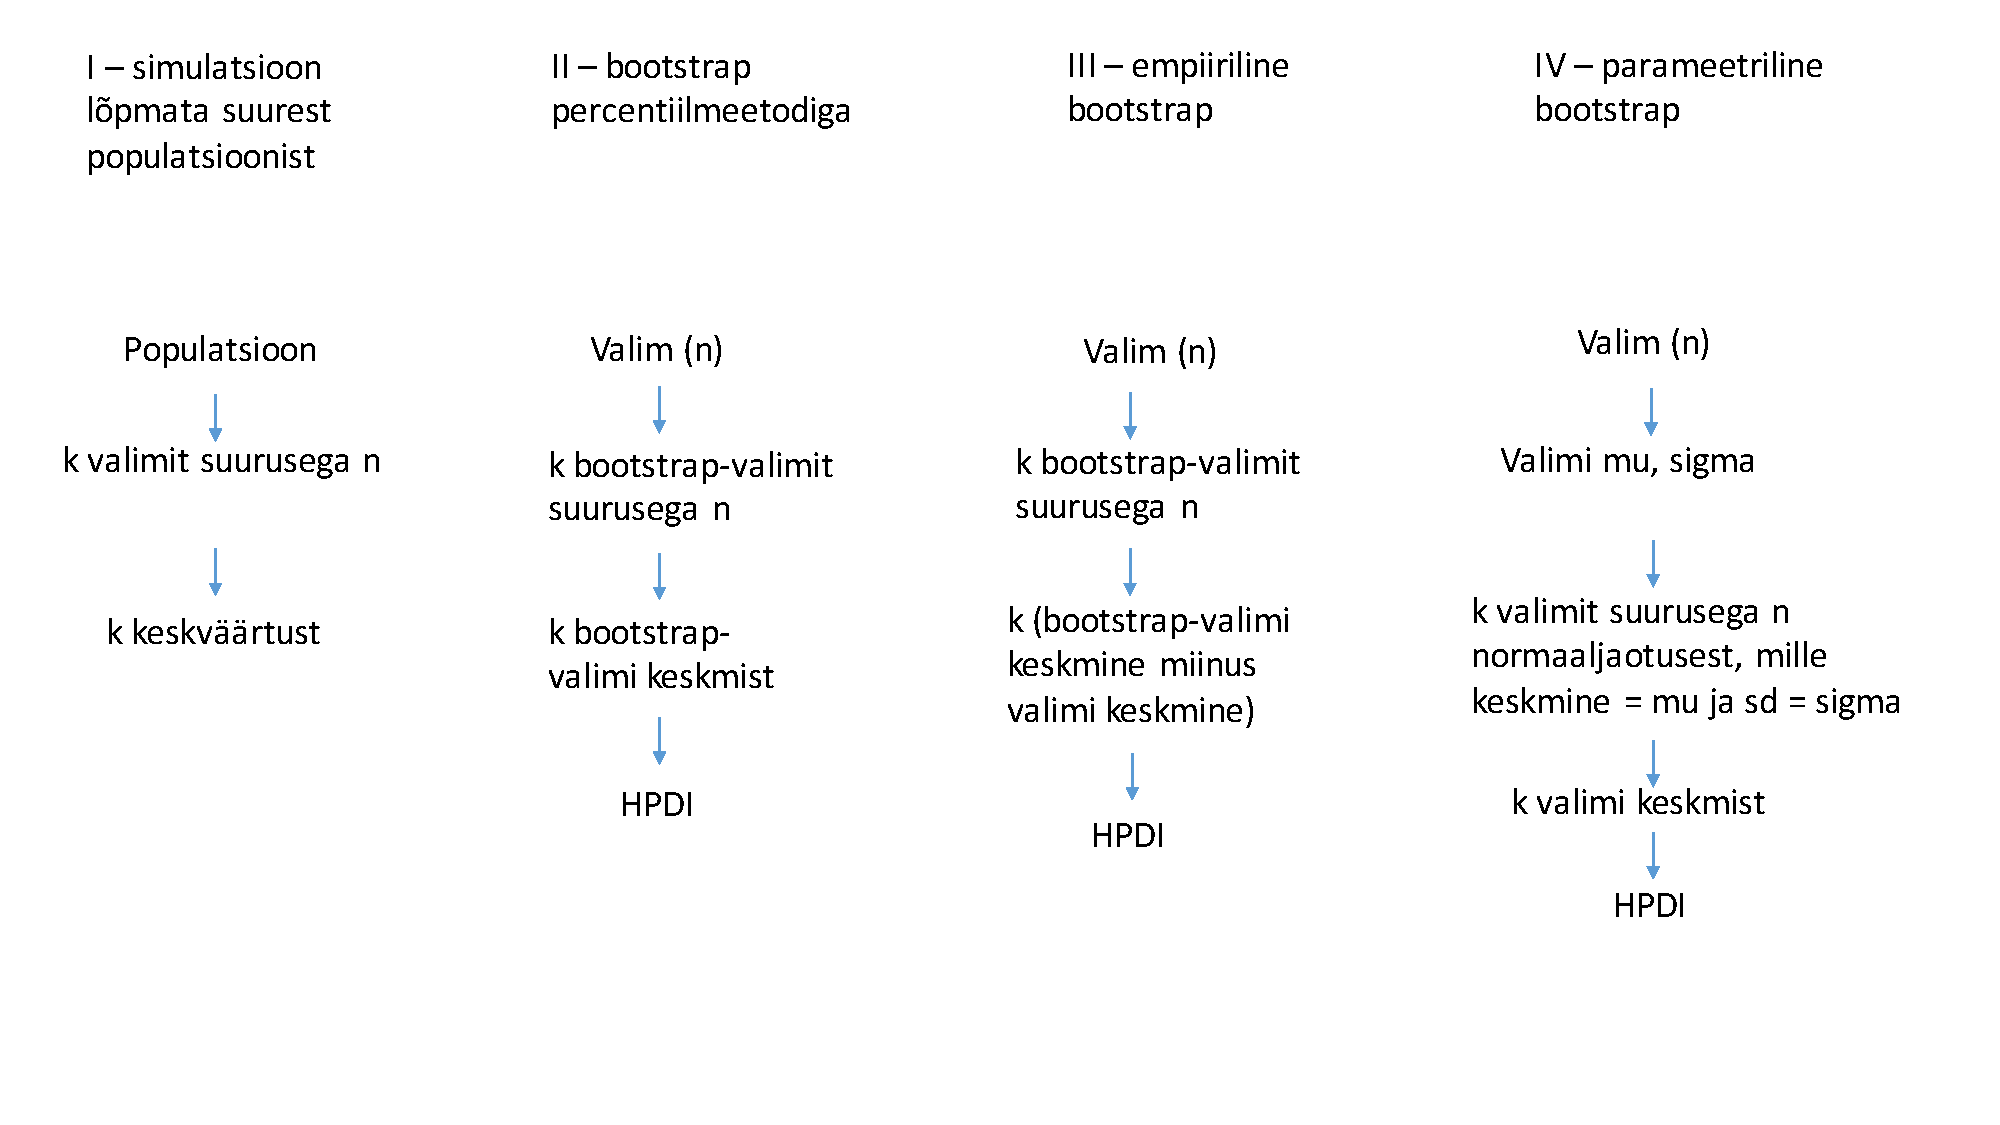
\includegraphics[width=0.5\linewidth]{img/boot1} \caption{Bootstrappimise meetodid.}\label{fig:bootmeth}
\end{figure}

\section*{Bootstrappimine ei ole kogu
tõde}\label{bootstrappimine-ei-ole-kogu-tode}
\addcontentsline{toc}{section}{Bootstrappimine ei ole kogu tõde}

Bootstrappimine on võimas ja väga laia kasutusalaga meetodite kogum.
Sellel on siiski üks oluline puudus. Nimelt arvestab bootstrap ainult
andmetega ja ignoreerib taustateadmisi (parameetriline bootstrap küll
eeldab taustateadmisetele tuginevalt jaotusmudelit, kuid ignoreerib kogu
muud taustateadmist). Miks on see probleem?

Mõtleme hetkeks sellele teadusliku meetodi osale, millel põhineb
suuresti näiteks Darwini liikide tekkimise argument. See on nn
\emph{inference to the best explanation}, mille kohaselt on eelistatud
see teooria, mis on parimas kooskõlas faktidega, ehk mille kehtimise
korral on meie andmete esinemine kõige tõenäolisem. Kui mõni hüpotees
omistab andmete esinemisele suure tõenäosuse, siis me ütleme tehnilises
keeles, et see hüpotees on tõepärane (\emph{has high likelihood}).
Esmapilgul tundub see kõik igati mõistlik, kuid proovime lihtsat
mõtteeksperimenti. Selles juhtub nii, et loteriil võidab peaauhinna
meile tundmatu kodanik Franz K. Meil on selle fakti (ehk nende andmete)
seletamiseks kaks teooriat: 1. Franz K. võit oli juhuslik (loterii oli
aus ja keegi peab ju võitma) ja 2. Franz K. noorem õde võltsis loterii
tulemusi oma venna kasuks. Teine teooria sobib andmetega palju paremini
kui esimene (sest kuigi keegi peab võitma, Franz K. võiduvõimalus oli
väga väike); aga ometi eelistab enamus mõistlikke inimesi esimest
teooriat. Põhjus on selles, et meil pole iseenesest mingit alust arvata,
et Franz K.-l üldse on noorem õde, või et see õde omaks ligipääsu
loteriile. Kui me aga saame teada, et Franz K. noorem õde tõesti
korraldab loteriid, siis leiame kohe, et asi on kahtlane.

Siit näeme, et lisaks tõepärale on selleks, et me usuksime mõne teooria
kehtimisse, vaja veel, et see teooria oleks piisavalt tõenäoline meie
taustateadmiste valguses. Bayesi teoreem ei tee muud, kui arvutab
teooria kehtimise posterioorse tõenäosuse (järeltõenäosuse), kasutades
selleks meie eelteadmiste ja tõepära kvantitatiivseid mudeleid. Seega,
Bayesi paradigmas ei arvesta me mitte ainult andmetega, vaid ka
taustateadmistega, sünteesides need kokku üheks posterioorseks jaotuseks
ehk järeljaotuseks. Selle jaotuse arvutamine erineb bootstrapist, kuid
tema tõlgendus ja praktiline töö sellega on sarnane. Erinevalt
tavapärasest bootstrapist on Bayes parameetriline meetod, mis sõltub
andmete modelleerimisest modeleerija poolt ette antud jaotustesse
(normaaljaotus, t jaotus jne). Tegelikult peame me Bayesi arvutuseks
modelleerima vähemalt kaks erinevat jaotust: andmete jaotus, mida me
kutsume likelihoodiks ehk tõepäraks, ning eelneva teadmise mudel ehk
prior, mida samuti modeleeritakse tõenäosusjaotusena.

\begin{quote}
Bootstrapil on mõned imelikud formaalsed eeldused: 1. väärtused, mis ei
esine valimiandmetes, on võimatud, 2. Väärtused, mis esinevad väljaspool
valimi väärtuste vahemikku, on võimatud, 3. andmetes ei esine
ajasõltuvusi ega hierarhilisi struktuure. Nendest puudustest hoolimata
kasutatakse bootstrappimist laialt ja edukalt --- eelkõige tema lihtsuse
ja paindlikuse tõttu. Küll aga tähendab see, et bootstrap on harva parim
võimalik meetod mingi ülesande lahendamiseks.
\end{quote}

Ehkki bootstrappimine ei arvesta taustateadmistega, ei tee seda olulisel
määral ka paljud Bayesi mudelid (mudeldaja vaba valiku tõttu, mitte
selle pärast, et mudel ei suudaks taustainfot inkorporeerida). Bayesi
meetodite väljatöötajad ei tea sageli ette, milliste teaduslike
probleemide lahendamiseks nende mudeleid hakatakse kasutama, ja seega ei
kirjuta nad mudelisse ka väga ranget eelteadmist. Nende mudelite
teadlastest kasutajad lepivad sageli selllega ja lasevad oma mudelite
kaudu ``andmetel kõneleda'' enam-vähem sellistena, nagu need juhtuvad
olema. Sellist lähenemist ei saa alati hukka mõista, sest vahest ei
olegi meil palju eelteadmisi oma probleemi kohta, küll aga tuleb
mainida, et sellistel juhtudel annab bootstrappimine sageli lihtsama
vaevaga väga sarnase tulemuse kui Bayesi täismäng.

\chapter{Bayesi põhimõte}\label{bayesi-pohimote}

Bayesi arvutuseks on meil vaja teada

\begin{enumerate}
\def\labelenumi{\arabic{enumi})}
\item
  milline on ``\emph{parameter space}'' ehk parameetriruum?
  Parameetriruum koosneb kõikidest loogiliselt võimalikest
  parameetriväärtustest. Näiteks kui me viskame ühe korra münti, koosneb
  parameetriruum kahest elemendist: 0 ja 1, ehk null kulli ja üks kull.
  See ammendab võimalike sündmuste nimekirja. Kui me aga hindame mõnd
  pidevat suurust (keskmine pikkus, tõenäosus 0 ja 1 vahel jms), koosneb
  parameetriruum lõpmata paljudest elementidest (arvudest).
\item
  milline on ``\emph{likelihood function}'' ehk tõepärafunktsioon? Me
  omistame igale parameetriruumi elemendile (igale võimalikule
  parameetri väärtusele) tõepära. Tõepära parameetri väärtusel x on
  tõenäosus, millega me võiksime kohata oma andmete keskväärtust, juhul
  kui x oleks see ainus päris õige parameetri väärtus. Teisisõnu,
  tõepära on kooskõla määr andmete ja parameetri väärtuse x vahel.
  Tõepära = \(P(andmed~\vert~parameetri~v\ddot{a}\ddot{a}rtus)\).
  Näiteks, kui tõenäolised on meie andmed, kui USA keskmine president on
  juhtumisi 183.83629 cm pikkune? Kuna meil on vaja modeleerida tõepära
  igal võimalikul parameetri väärtusel (mida pideva suuruse puhul on
  lõpmatu hulk), siis kujutame tõepära pideva funktsioonina (näiteks
  normaaljaotusena), mis täielikult katab parameetriruumi.
  Tõepärafunktsioon ei summeeru 100-le protsendile --- see on
  normaliseerimata.
\item
  milline on ``\emph{prior function}'' ehk prior? Igale tõepära
  väärtusele peab vastama priori väärtus. Seega, kui tõepära on
  modelleeritud pideva funktsioonina, siis on ka prior pidev funktsioon
  (aga prior ei pea olema sama tüüpi funktsioon, kui tõepära). Erinevus
  tõepära ja priori vahel seisneb selles, et kui tõepärafunktsioon annab
  just meie andmete keskväärtuse tõenäosuse igal parameetriväärtusel,
  siis prior annab iga parameetriväärtuse tõenäosuse, sõltumata meie
  andmetest. See-eest arvestab prior kõikide teiste relevantsete
  andmetega, sünteesides taustateadmised ühte tõenäousmudelisse. Me
  omistame igale parameetriruumi väärtusele eelneva tõenäosuse, et see
  väärtus on üks ja ainus tõene väärtus. Prior jaotus summeerub 1-le.
  Prior kajastab meie konkreetsetest andmetest sõltumatut arvamust, kui
  suure tõenäosusega on just see parameetri väärtus tõene; seega seda,
  mida me usume enne oma andmete nägemist. Nendel parameetri väärtustel,
  kus prior (või tõepära) = 0\%, on ka posteerior garanteeritult 0\%.
  See tähendab, et kui te olete 100\% kindel, et mingi sündmus on
  võimatu, siis ei suuda ka mäekõrgune hunnik uusi andmeid teie uskumust
  muuta (eelduselt, et te olete ratsionaalne inimene).
\end{enumerate}

\url{http://optics.eee.nottingham.ac.uk/match/uncertainty.php} aitab
praktikas priorit modelleerida (proovige \emph{Roulette} meetodit).

Kui te eelnevast päriselt aru ei saanud, ärge muretsege. Varsti tulevad
puust ja punaseks näited likelihoodi ja priori kohta.

Edasi on lihtne. Arvuti võtab tõepärafunktsiooni ja priori, korrutab
need üksteisega läbi ning seejärel normaliseerib saadud jaotuse nii, et
jaotusealune pindala võrdub ühega. Saadud tõenäosusjaotus ongi
posteeriorne jaotus ehk posteerior ehk järeljaotus. Kogu lugu.

Me teame juba pool sajandit, et Bayesi teoreem on sellisele ülesandele
parim võimalik lahendus. Lihtsamad ülesanded lahendame me selle abil
täiuslikult. Kuna parameetrite arvu kasvuga mudelis muutub Bayesi
teoreemi läbiarvutamine eksponentsiaalselt arvutusmahukamaks (sest läbi
tuleb arvutada mudeli kõikide parameetrite kõikide väärtuste
kõikvõimalikud kombinatsioonid), oleme sunnitud vähegi keerulisemad
ülesanded lahendama umbkaudu, asendades Bayesi teoreemi \emph{ad hoc}
MCMC algoritmiga, mis teie arvutis peituva propelleri Karlsoni kombel
lendu saadab, et tõmmata valim ``otse'' posterioorsest jaotusest. Meie
poolt kasutatava MCMC \emph{Hamiltonian Monte Carlo} mootori nimi on
Stan (www.mc-stan.org). See on eraldiseisev programm, millel on R-i
liides R-i pakettide rstan(), rethinking(), rstanarm() jt kaudu. Meie
töötame ka edaspidi puhtalt R-s, mis automaatselt suunab meie mudelid ja
muud andmed Stani, kus need läbi arvutatakse ja seejärel tulemused R-i
tagasi saadetakse. Tulemuste töötlus ja graafiline esitus toimub jällegi
R-is. Seega ei pea me ise kordagi Stani avama.

Alustame siiski lihtsa näitega, mida saab käsitsi läbi arvutada.

\section*{Esimene näide}\label{esimene-naide}
\addcontentsline{toc}{section}{Esimene näide}

Me teame, et suremus haigusesse on 50\% ja meil on palatis 3 patsienti,
kes seda haigust põevad. Seega on meil kaks andmetükki (50\% ja n=3).
Küsimus: mitu meie patsienti oodatavalt hinge heidavad? Eeldusel, et
meie patsiendid on iseseisvad (näiteks ei ole sugulased), on meil
tüüpiline mündiviske olukord.

Parameetriruum on neljaliikmeline: 0 surnud, 1 surnud, 2 surnud ja 3
surnud. Edasi loeme üles kõik võimalikud sündmusteahelad, mis
loogiliselt saavad juhtuda, et saada tõepärafunktsioon.

Me viskame kulli-kirja 3 korda: kiri = elus, kull = surnud

Võimalikud sündmused on: \textbar{} kull kull kull \textbar{} kull kiri
kull \textbar{} kiri kull kull \textbar{} kull kull kiri \textbar{} kull
kiri kiri \textbar{} kiri kiri kull \textbar{} kiri kull kiri \textbar{}
kiri kiri kiri

Kui P(kull) = 0.5, siis lugedes kokku kõik võimalikud sündmused:

\begin{itemize}
\tightlist
\item
  0 kulli ehk surnud - 1,
\item
  1 kulli ehk surnud - 3,
\item
  2 kulli ehk surnud - 3,
\item
  3 kulli ehk surnud - 1
\end{itemize}

Nüüd teame parameetriruumi iga liikme kohta, kui suure tõenäosusega me
ootame selle realiseerumist. Näiteks, P(0 surnud) = 1/8, P(1 surnud) =
3/8, P(1 või 2 surnud) = 6/8 jne Selle teadmise konverteerime
tõepärafunktsiooniks.

\begin{Shaded}
\begin{Highlighting}[]
\KeywordTok{library}\NormalTok{(tidyverse)}
\CommentTok{# Parameter space: all possible futures}
\NormalTok{x <-}\StringTok{ }\KeywordTok{seq}\NormalTok{(}\DataTypeTok{from =} \DecValTok{0}\NormalTok{, }\DataTypeTok{to =} \DecValTok{3}\NormalTok{)}

\CommentTok{# Likelihoods for each x value, or P(deaths I x)}
\NormalTok{y <-}\StringTok{ }\KeywordTok{c}\NormalTok{(}\DecValTok{1}\NormalTok{, }\DecValTok{3}\NormalTok{, }\DecValTok{3}\NormalTok{, }\DecValTok{1}\NormalTok{)}

\KeywordTok{ggplot}\NormalTok{(}\DataTypeTok{data=}\OtherTok{NULL}\NormalTok{, }\KeywordTok{aes}\NormalTok{(x, y)) }\OperatorTok{+}\StringTok{ }
\StringTok{  }\KeywordTok{geom_point}\NormalTok{()}\OperatorTok{+}\StringTok{ }
\StringTok{  }\KeywordTok{geom_line}\NormalTok{()}\OperatorTok{+}
\StringTok{  }\KeywordTok{xlab}\NormalTok{(}\StringTok{"hypothetical nr of deaths"}\NormalTok{)}\OperatorTok{+}\StringTok{ }
\StringTok{  }\KeywordTok{ylab}\NormalTok{(}\StringTok{"plausibility"}\NormalTok{)}
\end{Highlighting}
\end{Shaded}

\includegraphics{10_bayesi_printsiip_files/figure-latex/unnamed-chunk-2-1.pdf}

Siit näeme, et üks surm ja kaks surma on sama tõenäolised ja üks surm on
kolm korda tõenäolisem kui null surma (või kolm surma). Tõepära annab
meile tõenäosuse Pr(mortality=0.5 \& N=3) igale loogiliselt võimalikule
surmade arvule (0 kuni 3).

Me saame sama tulemuse kasutades formaalsel viisil binoomjaotuse
mudelit. Ainus erinevus on, et nüüd on meil y teljel surmade tõenäosus.

\begin{Shaded}
\begin{Highlighting}[]
\NormalTok{y <-}\StringTok{ }\KeywordTok{dbinom}\NormalTok{(x, }\DecValTok{3}\NormalTok{, }\FloatTok{0.5}\NormalTok{)}

\KeywordTok{ggplot}\NormalTok{(}\DataTypeTok{data=}\OtherTok{NULL}\NormalTok{, }\KeywordTok{aes}\NormalTok{(x, y)) }\OperatorTok{+}\StringTok{ }
\StringTok{  }\KeywordTok{geom_point}\NormalTok{()}\OperatorTok{+}
\StringTok{  }\KeywordTok{geom_line}\NormalTok{()}\OperatorTok{+}
\StringTok{  }\KeywordTok{xlab}\NormalTok{(}\StringTok{"hypothetical nr of deaths"}\NormalTok{)}\OperatorTok{+}\StringTok{ }
\StringTok{  }\KeywordTok{ylab}\NormalTok{(}\StringTok{"probability"}\NormalTok{)}
\end{Highlighting}
\end{Shaded}

\includegraphics{10_bayesi_printsiip_files/figure-latex/unnamed-chunk-3-1.pdf}

Proovime seda koodi olukorras, kus meil on 9 patsienti ja suremus on
0.67:

\begin{Shaded}
\begin{Highlighting}[]
\NormalTok{x <-}\StringTok{ }\KeywordTok{seq}\NormalTok{(}\DataTypeTok{from =} \DecValTok{0}\NormalTok{, }\DataTypeTok{to =} \DecValTok{9}\NormalTok{)}
\NormalTok{y <-}\StringTok{ }\KeywordTok{dbinom}\NormalTok{(x, }\DecValTok{9}\NormalTok{, }\FloatTok{0.67}\NormalTok{)}

\KeywordTok{ggplot}\NormalTok{(}\DataTypeTok{data=}\OtherTok{NULL}\NormalTok{, }\KeywordTok{aes}\NormalTok{(x, y)) }\OperatorTok{+}\StringTok{ }
\StringTok{  }\KeywordTok{geom_point}\NormalTok{()}\OperatorTok{+}
\StringTok{  }\KeywordTok{geom_line}\NormalTok{()}\OperatorTok{+}
\StringTok{  }\KeywordTok{xlab}\NormalTok{(}\StringTok{"hypothetical nr of deaths"}\NormalTok{)}\OperatorTok{+}\StringTok{ }
\StringTok{  }\KeywordTok{ylab}\NormalTok{(}\StringTok{"probability"}\NormalTok{)}
\end{Highlighting}
\end{Shaded}

\includegraphics{10_bayesi_printsiip_files/figure-latex/unnamed-chunk-4-1.pdf}

Lisame sellele tõepärafunktsioonile tasase priori (lihtsuse huvides) ja
arvutame posterioorse jaotuse kasutades Bayesi teoreemi. Igale
parameetri väärtusele on tõepära * prior proportsionaalne posterioorse
tõenäosusega, et just see parameetri väärtus on see ainus tõene väärtus.
Posterioorsed tõenäosused normaliseeritakse nii, et nad summeeruksid
1-le.

Me defineerime X telje kui rea 10-st arvust (0 kuni 9 surma) ja arvutame
tõepära igale neist 10-st arvust. Sellega ammendame me kõik loogiliselt
võimalikud parameetri väärtused.



\begin{Shaded}
\begin{Highlighting}[]
\NormalTok{x <-}\StringTok{ }\KeywordTok{seq}\NormalTok{(}\DataTypeTok{from =} \DecValTok{0}\NormalTok{ , }\DataTypeTok{to =} \DecValTok{9}\NormalTok{)}
\CommentTok{# flat prior}
\NormalTok{prior <-}\StringTok{ }\KeywordTok{rep}\NormalTok{(}\DecValTok{1}\NormalTok{ , }\DecValTok{10}\NormalTok{)}

\CommentTok{# Compute likelihood at each value in grid}
\NormalTok{likelihood <-}\StringTok{ }\KeywordTok{dbinom}\NormalTok{(x, }\DataTypeTok{size =} \DecValTok{9}\NormalTok{, }\DataTypeTok{prob =} \FloatTok{0.67}\NormalTok{)}

\CommentTok{# Compute product of likelihood and prior}
\NormalTok{unstd.posterior <-}\StringTok{ }\NormalTok{likelihood }\OperatorTok{*}\StringTok{ }\NormalTok{prior}

\CommentTok{# Normalize the posterior, so that it sums to 1}
\NormalTok{posterior <-}\StringTok{ }\NormalTok{unstd.posterior }\OperatorTok{/}\StringTok{ }\KeywordTok{sum}\NormalTok{(unstd.posterior)}

\KeywordTok{ggplot}\NormalTok{(}\DataTypeTok{data =} \OtherTok{NULL}\NormalTok{, }\KeywordTok{aes}\NormalTok{(x, posterior)) }\OperatorTok{+}\StringTok{ }
\StringTok{  }\KeywordTok{geom_point}\NormalTok{() }\OperatorTok{+}
\StringTok{  }\KeywordTok{geom_line}\NormalTok{() }\OperatorTok{+}
\StringTok{  }\KeywordTok{xlab}\NormalTok{(}\StringTok{"hypothetical nr of deaths"}\NormalTok{) }\OperatorTok{+}\StringTok{ }
\StringTok{  }\KeywordTok{ylab}\NormalTok{(}\StringTok{"posterior probability"}\NormalTok{)}
\end{Highlighting}
\end{Shaded}

\includegraphics{10_bayesi_printsiip_files/figure-latex/unnamed-chunk-5-1.pdf}

See on parim võimalik teadmine, mitu kirstu tasuks tellida, arvestades
meie priori ja likelihoodi mudelitega. Näiteks, sedapalju, kui surmad ei
ole üksteisest sõltumatud, on meie tõepäramudel (binoomjaotus) vale.

\section*{Teine näide: sõnastame oma probleemi
ümber}\label{teine-naide-sonastame-oma-probleemi-umber}
\addcontentsline{toc}{section}{Teine näide: sõnastame oma probleemi
ümber}

Mis siis, kui me ei tea suremust ja tahaksime seda välja arvutada? Kõik,
mida me teame on, et 6 patsienti 9st surid. Nüüd koosnevad andmed 9
patsiendi mortaalsusinfost (parameeter, mille väärtust me eelmises
näites arvutasime) ja parameeter, mille väärtust me ei tea, on surmade
üldine sagedus (see parameeter oli eelmises näites fikseeritud, ja seega
kuulus andmete hulka).

Seega on meil:

\begin{enumerate}
\def\labelenumi{\arabic{enumi}.}
\item
  Parameetriruum 0\% kuni 100\% suremus (0st 1-ni), mis sisaldab lõpmata
  palju numbreid.
\item
  Kaks võimalikku sündmust (surnud, elus), seega binoomjaotusega
  modelleeritud tõepärafunktsioon. Nagu me juba teame, on r funktsioonis
  dbinom() kolm argumenti: surmade arv, patsientide koguarv ja surmade
  tõenäosus. Seekord oleme me fikseerinud esimesed kaks ja soovime
  arvutada kolmanda väärtuse.
\item
  Tasane prior, mis ulatub 0 ja 1 vahel. Me valisime selle priori
  selleks, et mitte muuta tõepärafunktsiooni kuju. See ei tähenda, et me
  arvaksime, et tasane prior on mitteinformatiivne. Tasane prior
  tähendab, et me usume, et suremuse kõik väärtused 0 ja 1 vahel on
  võrdselt tõenäolised. See on vägagi informatsioonirohke (ebatavaline)
  viis maailma näha, ükskõik mis haiguse puhul!
\end{enumerate}

\textbf{Tõepära parameetri väärtusel x on tõenäosus kohata meie andmeid,
kui x on juhtumisi parameetri tegelik väärtus.} Meie näites koosneb
tõepärafunktsioon tõenäosustest, et kuus üheksast patsiendist surid igal
võimalikul suremuse väärtusel (0\ldots{}1). Kuna see on lõpmatu rida,
teeme natuke sohki ja arvutame tõepära 20-l valitud suremuse väärtusel.

\begin{quote}
Tehniliselt on sinu andmete tõepärafunktsioon agregeeritud iga üksiku
andmepunkti tõepärafunktsioonist. Seega vaatab Bayes igat andmepunkti
eraldi (andmete sisestamise järjekord ei loe).
\end{quote}



\begin{Shaded}
\begin{Highlighting}[]
\CommentTok{# mortality at 20 evenly spaced probabilities from 0 to 1}
\NormalTok{x <-}\StringTok{ }\KeywordTok{seq}\NormalTok{(}\DataTypeTok{from =} \DecValTok{0}\NormalTok{ , }\DataTypeTok{to =} \DecValTok{1}\NormalTok{, }\DataTypeTok{length.out =} \DecValTok{20}\NormalTok{)}

\CommentTok{# Define prior}
\NormalTok{prior <-}\StringTok{ }\KeywordTok{rep}\NormalTok{(}\DecValTok{1}\NormalTok{ , }\DecValTok{20}\NormalTok{)}

\CommentTok{# Compute likelihood at each value in grid}
\NormalTok{likelihood <-}\StringTok{ }\KeywordTok{dbinom}\NormalTok{(}\DecValTok{6}\NormalTok{, }\DataTypeTok{size =} \DecValTok{9}\NormalTok{ , }\DataTypeTok{prob =}\NormalTok{ x)}

\CommentTok{# Compute product of likelihood and prior & standardize the posterior}
\NormalTok{posterior <-}\StringTok{ }\NormalTok{likelihood }\OperatorTok{*}\StringTok{ }\NormalTok{prior }\OperatorTok{/}\StringTok{ }\KeywordTok{sum}\NormalTok{(likelihood }\OperatorTok{*}\StringTok{ }\NormalTok{prior)}

\CommentTok{#put everithing into a tibble for plotting}
\NormalTok{a <-}\StringTok{ }\KeywordTok{tibble}\NormalTok{(}\DataTypeTok{x=}\KeywordTok{rep}\NormalTok{(}\DataTypeTok{x=}\NormalTok{x, }\DecValTok{3}\NormalTok{),}
            \DataTypeTok{y=} \KeywordTok{c}\NormalTok{(prior, likelihood, posterior),}
            \DataTypeTok{legend=} \KeywordTok{rep}\NormalTok{(}\KeywordTok{c}\NormalTok{(}\StringTok{"prior"}\NormalTok{,}\StringTok{"likelihood"}\NormalTok{, }\StringTok{"posterior"}\NormalTok{), }\DataTypeTok{each=}\DecValTok{20}\NormalTok{))}

\KeywordTok{ggplot}\NormalTok{(}\DataTypeTok{data=}\NormalTok{a) }\OperatorTok{+}\StringTok{ }\KeywordTok{geom_line}\NormalTok{(}\KeywordTok{aes}\NormalTok{(x, y, }\DataTypeTok{color=}\NormalTok{legend))}
\end{Highlighting}
\end{Shaded}

\includegraphics{10_bayesi_printsiip_files/figure-latex/unnamed-chunk-6-1.pdf}

Nüüd on meil posterioorne tõenäosusfunktsioon, mis summeerub 1-le ja mis
sisaldab kogu meie teadmist suremuse kohta.

\begin{quote}
Alati on kasulik plottida kõik kolm funktsiooni (tõepära, prior ja
posteerior).
\end{quote}

\section*{Kui n = 1}\label{kui-n-1}
\addcontentsline{toc}{section}{Kui n = 1}

Bayes on lahe sest tema hinnangud väiksele N-le on loogiliselt sama
pädevad kui suurele N-le. See ei ole nii klassikalises sageduslikus
statistikas, kus paljud testid on välja töötatud N = Inf eeldusel ja
töötavad halvasti väikeste valimitega.

Hea küll, me arvutame jälle suremust.

Bayes töötab andmepunkti kaupa (see et me talle ennist kõik andmed
korraga ette andsime, on puhtalt mugavuse pärast).



\begin{Shaded}
\begin{Highlighting}[]
\CommentTok{# Define grid}
\NormalTok{x <-}\StringTok{ }\KeywordTok{seq}\NormalTok{(}\DataTypeTok{from =} \DecValTok{0}\NormalTok{, }\DataTypeTok{to =} \DecValTok{1}\NormalTok{, }\DataTypeTok{length.out =} \DecValTok{20}\NormalTok{)}

\CommentTok{# Define prior}
\NormalTok{prior <-}\StringTok{ }\KeywordTok{rep}\NormalTok{(}\DecValTok{1}\NormalTok{, }\DecValTok{20}\NormalTok{)}

\CommentTok{# Compute likelihood at each value in grid}
\NormalTok{likelihood <-}\StringTok{ }\KeywordTok{dbinom}\NormalTok{(}\DecValTok{1}\NormalTok{, }\DataTypeTok{size =} \DecValTok{1}\NormalTok{, }\DataTypeTok{prob =}\NormalTok{ x)}
\NormalTok{posterior <-}\StringTok{ }\NormalTok{likelihood }\OperatorTok{*}\StringTok{ }\NormalTok{prior }\OperatorTok{/}\StringTok{ }\KeywordTok{sum}\NormalTok{(likelihood }\OperatorTok{*}\StringTok{ }\NormalTok{prior)}

\KeywordTok{ggplot}\NormalTok{(}\DataTypeTok{data=}\OtherTok{NULL}\NormalTok{)}\OperatorTok{+}
\StringTok{  }\KeywordTok{geom_line}\NormalTok{(}\KeywordTok{aes}\NormalTok{(x, posterior), }\DataTypeTok{color=} \StringTok{"blue"}\NormalTok{)}
\end{Highlighting}
\end{Shaded}

\begin{figure}
\centering
\includegraphics{10_bayesi_printsiip_files/figure-latex/esimene-patsient-1.pdf}
\caption{\label{fig:esimene-patsient}N=1, esimene patsient suri.}
\end{figure}

Esimene patsient suri - 0 mortaalsus ei ole enam loogiliselt võimalik
(välja arvatud siis kui prior selle koha peal = 0) ja mortaalsus 100\%
on andmetega (tegelikult andmega) parimini kooskõlas. Posteerior on
nulli ja 100\% vahel sirge sest vähene sissepandud informatsioon
lihtsalt ei võimalda enamat.



\begin{Shaded}
\begin{Highlighting}[]
\NormalTok{x <-}\StringTok{ }\KeywordTok{seq}\NormalTok{(}\DataTypeTok{from =} \DecValTok{0}\NormalTok{, }\DataTypeTok{to =} \DecValTok{1}\NormalTok{, }\DataTypeTok{length.out =} \DecValTok{20}\NormalTok{)}
\CommentTok{# Define prior}
\NormalTok{prior <-}\StringTok{ }\NormalTok{posterior}

\CommentTok{# Compute likelihood at each value in grid}
\NormalTok{likelihood <-}\StringTok{ }\KeywordTok{dbinom}\NormalTok{(}\DecValTok{1}\NormalTok{ , }\DataTypeTok{size =} \DecValTok{1}\NormalTok{, }\DataTypeTok{prob =}\NormalTok{ x)}
\NormalTok{posterior1 <-}\StringTok{ }\NormalTok{likelihood }\OperatorTok{*}\StringTok{ }\NormalTok{prior }\OperatorTok{/}\StringTok{ }\KeywordTok{sum}\NormalTok{(likelihood }\OperatorTok{*}\StringTok{ }\NormalTok{prior)}

\KeywordTok{ggplot}\NormalTok{(}\DataTypeTok{data=}\OtherTok{NULL}\NormalTok{)}\OperatorTok{+}
\StringTok{  }\KeywordTok{geom_line}\NormalTok{(}\KeywordTok{aes}\NormalTok{(x, prior))}\OperatorTok{+}
\StringTok{  }\KeywordTok{geom_line}\NormalTok{(}\KeywordTok{aes}\NormalTok{(x, posterior1), }\DataTypeTok{color=}\StringTok{"blue"}\NormalTok{)}
\end{Highlighting}
\end{Shaded}

\begin{figure}
\centering
\includegraphics{10_bayesi_printsiip_files/figure-latex/teine-patsient-1.pdf}
\caption{\label{fig:teine-patsient}N=2, teine patsient suri.}
\end{figure}

Teine patsient suri. Nüüd ei ole 0 ja 1 vahel enam sirge posteerior.
Posteerior on kaldu 100 protsendi poole, mis on ikka kõige tõenäolisem
väärtus.



\begin{Shaded}
\begin{Highlighting}[]
\NormalTok{x <-}\StringTok{ }\KeywordTok{seq}\NormalTok{(}\DataTypeTok{from =} \DecValTok{0}\NormalTok{, }\DataTypeTok{to =} \DecValTok{1}\NormalTok{, }\DataTypeTok{length.out =} \DecValTok{20}\NormalTok{)}
\CommentTok{# Define prior}
\NormalTok{prior <-}\StringTok{ }\NormalTok{posterior1}

\CommentTok{# Compute likelihood at each value in grid}
\NormalTok{likelihood <-}\StringTok{ }\KeywordTok{dbinom}\NormalTok{(}\DecValTok{0}\NormalTok{, }\DataTypeTok{size =} \DecValTok{1}\NormalTok{, }\DataTypeTok{prob =}\NormalTok{ x)}

\CommentTok{# Compute product of likelihood and prior}
\NormalTok{posterior2 <-}\StringTok{ }\NormalTok{likelihood }\OperatorTok{*}\StringTok{ }\NormalTok{prior }\OperatorTok{/}\StringTok{ }\KeywordTok{sum}\NormalTok{(likelihood }\OperatorTok{*}\StringTok{ }\NormalTok{prior)}

\KeywordTok{ggplot}\NormalTok{(}\DataTypeTok{data=}\OtherTok{NULL}\NormalTok{)}\OperatorTok{+}
\StringTok{  }\KeywordTok{geom_line}\NormalTok{(}\KeywordTok{aes}\NormalTok{(x, prior))}\OperatorTok{+}
\StringTok{  }\KeywordTok{geom_line}\NormalTok{(}\KeywordTok{aes}\NormalTok{(x, posterior2), }\DataTypeTok{color=}\StringTok{"blue"}\NormalTok{)}
\end{Highlighting}
\end{Shaded}

\begin{figure}
\centering
\includegraphics{10_bayesi_printsiip_files/figure-latex/kolmas-patsient-1.pdf}
\caption{\label{fig:kolmas-patsient}N=3, kolmas patsient jäi ellu.}
\end{figure}

Kolmas patsient jäi ellu - 0 ja 100\% mortaalsus on seega võimaluste
nimekirjast maas ning suremus on ikka kaldu valimi keskmise poole
(75\%).

Teeme sedasama prioriga, mis ei ole tasane. See illustreerib tõsiasja,
et kui N on väike siis domineerib prior posteerior jaotust. (Suure N
korral on vastupidi, priori kuju on sageli vähetähtis.)



\begin{Shaded}
\begin{Highlighting}[]
\NormalTok{x <-}\StringTok{ }\KeywordTok{seq}\NormalTok{(}\DataTypeTok{from =} \DecValTok{0}\NormalTok{, }\DataTypeTok{to =} \DecValTok{1}\NormalTok{, }\DataTypeTok{length.out =} \DecValTok{20}\NormalTok{)}
\CommentTok{# Define prior}
\NormalTok{prior <-}\StringTok{ }\KeywordTok{c}\NormalTok{(}\KeywordTok{seq}\NormalTok{(}\FloatTok{0.01}\NormalTok{, }\FloatTok{0.1}\NormalTok{, }\DataTypeTok{length.out =} \DecValTok{10}\NormalTok{), }\KeywordTok{seq}\NormalTok{(}\FloatTok{0.1}\NormalTok{, }\FloatTok{0.01}\NormalTok{, }\DataTypeTok{length.out =} \DecValTok{10}\NormalTok{))}

\CommentTok{# Compute likelihood at each value in grid}
\NormalTok{likelihood <-}\StringTok{ }\KeywordTok{dbinom}\NormalTok{(}\DecValTok{1}\NormalTok{, }\DataTypeTok{size =} \DecValTok{1}\NormalTok{ , }\DataTypeTok{prob =}\NormalTok{ x)}
\NormalTok{posterior <-}\StringTok{ }\NormalTok{likelihood }\OperatorTok{*}\StringTok{ }\NormalTok{prior }\OperatorTok{/}\StringTok{ }\KeywordTok{sum}\NormalTok{(likelihood }\OperatorTok{*}\StringTok{ }\NormalTok{prior)}

\KeywordTok{ggplot}\NormalTok{(}\DataTypeTok{data=}\OtherTok{NULL}\NormalTok{)}\OperatorTok{+}
\StringTok{  }\KeywordTok{geom_line}\NormalTok{(}\KeywordTok{aes}\NormalTok{(x, prior))}\OperatorTok{+}
\StringTok{  }\KeywordTok{geom_line}\NormalTok{(}\KeywordTok{aes}\NormalTok{(x, likelihood), }\DataTypeTok{color=}\StringTok{"red"}\NormalTok{)}\OperatorTok{+}
\StringTok{  }\KeywordTok{geom_line}\NormalTok{(}\KeywordTok{aes}\NormalTok{(x, posterior), }\DataTypeTok{color=}\StringTok{"blue"}\NormalTok{)}
\end{Highlighting}
\end{Shaded}

\includegraphics{10_bayesi_printsiip_files/figure-latex/unnamed-chunk-7-1.pdf}
1. patsient suri



\begin{Shaded}
\begin{Highlighting}[]
\CommentTok{# Define prior}
\NormalTok{prior <-}\StringTok{ }\NormalTok{posterior}

\CommentTok{# Compute likelihood at each value in grid}
\NormalTok{likelihood <-}\StringTok{ }\KeywordTok{dbinom}\NormalTok{(}\DecValTok{2}\NormalTok{, }\DataTypeTok{size =} \DecValTok{2}\NormalTok{, }\DataTypeTok{prob =}\NormalTok{ x)}

\CommentTok{# Compute product of likelihood and prior}
\NormalTok{posterior1 <-}\StringTok{ }\NormalTok{likelihood }\OperatorTok{*}\StringTok{ }\NormalTok{prior }\OperatorTok{/}\StringTok{ }\KeywordTok{sum}\NormalTok{(likelihood }\OperatorTok{*}\StringTok{ }\NormalTok{prior)}

\KeywordTok{ggplot}\NormalTok{(}\DataTypeTok{data=}\OtherTok{NULL}\NormalTok{)}\OperatorTok{+}
\StringTok{  }\KeywordTok{geom_line}\NormalTok{(}\KeywordTok{aes}\NormalTok{(x, prior))}\OperatorTok{+}
\StringTok{  }\KeywordTok{geom_line}\NormalTok{(}\KeywordTok{aes}\NormalTok{(x, likelihood), }\DataTypeTok{color=}\StringTok{"red"}\NormalTok{)}\OperatorTok{+}
\StringTok{  }\KeywordTok{geom_line}\NormalTok{(}\KeywordTok{aes}\NormalTok{(x, posterior1), }\DataTypeTok{color=}\StringTok{"blue"}\NormalTok{)}
\end{Highlighting}
\end{Shaded}

\begin{figure}
\centering
\includegraphics{10_bayesi_printsiip_files/figure-latex/fuck-1.pdf}
\caption{\label{fig:fuck}N=2 informatiivse prioriga.}
\end{figure}

Teine patsient suri.



\begin{Shaded}
\begin{Highlighting}[]
\CommentTok{# Define prior}
\NormalTok{prior2 <-}\StringTok{ }\NormalTok{posterior1}

\CommentTok{# Compute likelihood at each value in grid}
\NormalTok{likelihood <-}\StringTok{ }\KeywordTok{dbinom}\NormalTok{(}\DecValTok{2}\NormalTok{, }\DataTypeTok{size =} \DecValTok{3}\NormalTok{, }\DataTypeTok{prob =}\NormalTok{ x)}

\CommentTok{# Compute product of likelihood and prior}
\NormalTok{posterior2 <-}\StringTok{ }\NormalTok{likelihood }\OperatorTok{*}\StringTok{ }\NormalTok{prior2 }\OperatorTok{/}\StringTok{ }\KeywordTok{sum}\NormalTok{(likelihood }\OperatorTok{*}\StringTok{ }\NormalTok{prior2)}

\KeywordTok{ggplot}\NormalTok{(}\DataTypeTok{data=}\OtherTok{NULL}\NormalTok{)}\OperatorTok{+}
\StringTok{  }\KeywordTok{geom_line}\NormalTok{(}\KeywordTok{aes}\NormalTok{(x, prior2))}\OperatorTok{+}
\StringTok{  }\KeywordTok{geom_line}\NormalTok{(}\KeywordTok{aes}\NormalTok{(x, likelihood), }\DataTypeTok{color=}\StringTok{"red"}\NormalTok{)}\OperatorTok{+}
\StringTok{  }\KeywordTok{geom_line}\NormalTok{(}\KeywordTok{aes}\NormalTok{(x, posterior2), }\DataTypeTok{color=}\StringTok{"blue"}\NormalTok{)}
\end{Highlighting}
\end{Shaded}

\includegraphics{10_bayesi_printsiip_files/figure-latex/omg-1.pdf}
Kolmas patsient jäi ellu. Nüüd on posteeriori tipp mitte 75\% juures
nagu ennist, vaid kuskil 50\% juures --- tänu priorile.

\chapter{Mudelite keel}\label{mudelite-keel}

Siin vaatame kuidas kirjeldada mudelit nii, et masin selle ära tunneb.
Meie mudelid töötavad läbi ``rethinking'' paketi. See raamatukogu pakub
kaks võimalust, kuidas mudelit arvutada, mis mõlemad kasutavad sama
notatsiooni. Mõlemad võimalused arvutavad posteeriori mitte Bayesi
teoreemi kasutades (nagu me ennist tegime), vaid kasutades stohhastilisi
meetodeid, mis iseloomustavad posteeriori umbkaudu (aga piisavalt
täpselt). Põhjuseks on, et keerulisemate mudelite korral on Bayesi
teoreemi kasutamine liialt arvutusmahukas.

Esiteks \texttt{rethinking::map()} leiab posteeriori tipu ja selle
lähedal funktsiooni tõusunurga. Siin on eelduseks, et posteerior on
normaaljaotus. See eeldus kehtib alati, kui nii prior kui tõepära on
modelleeritud normaaljaotusena (ja ka paljudel muudel juhtudel).

Teine võimalus on \texttt{rethinking::map2stan()}, mis suunab teie
kirjutatud mudeli Stan-i. Stan teeb \emph{Hamilonian Monte Carlo}
simulatsiooni, kasutades valget maagiat selleks, et tõmmata valim otse
posteerioorsest jaotusest. See on väga moodne lähenemine statistikale,
töötab oluliselt aeglasemalt kui map, aga ei sõltu normaaljaotustest
ning suudab arvutada hierarhilisi mudeleid, mis map-le üle jõu käivad.

Me võime sama mudeli kirjelduse sööta mõlemasse funktsiooni.

Lihtne mudel näeb välja niimodi:

\begin{verbatim}
dead ~ dbinom(9, p) # binomial likelihood
p ~ dunif(0, 1) # uniform prior
\end{verbatim}

Tõepärafunktsioon on modeleeritud binoomjaotusena. Parameeter, mille
väärtust määratakse on p, ehk suremus. See on ainus parameeter, mille
väärtust me siin krutime. NB! igale parameetrile peab vastama oma prior.
Meil on selles mudelis täpselt 1 parameeter ja 1 prior. Vastuseks saame
selle ainsa parameetri posterioorse jaotuse. Hiljem näeme, et kui meil
on näiteks 452 parameetrit, mille väärtusi me koos arvutame, siis on
meil ka 452 priorit ja 452 posterioorset jaotust.

\begin{Shaded}
\begin{Highlighting}[]
\KeywordTok{library}\NormalTok{(rethinking)}
\CommentTok{# Fit model using rethinking}
\NormalTok{m1 <-}\StringTok{ }\KeywordTok{map}\NormalTok{(}
    \KeywordTok{alist}\NormalTok{(}
\NormalTok{        dead }\OperatorTok{~}\StringTok{ }\KeywordTok{dbinom}\NormalTok{(}\DecValTok{9}\NormalTok{, p), }\CommentTok{# Binomial likelihood}
\NormalTok{        p }\OperatorTok{~}\StringTok{ }\KeywordTok{dunif}\NormalTok{(}\DecValTok{0}\NormalTok{, }\DecValTok{1}\NormalTok{) }\CommentTok{# Uniform prior}
\NormalTok{), }\DataTypeTok{data =} \KeywordTok{list}\NormalTok{(}\DataTypeTok{dead =} \DecValTok{6}\NormalTok{))}

\CommentTok{# Summary of quadratic approximation}
\KeywordTok{precis}\NormalTok{(m1)}
\CommentTok{#>   Mean StdDev 5.5% 94.5%}
\CommentTok{#> p 0.67   0.16 0.42  0.92}
\end{Highlighting}
\end{Shaded}

Nüüd tõmbame posteerioroorsest jaotusest valimi n=10 000. Selleks on
funktsioon extract.samples()



\begin{Shaded}
\begin{Highlighting}[]
\NormalTok{samples <-}\StringTok{ }\KeywordTok{extract.samples}\NormalTok{(m1)}
\CommentTok{# hist(samples$p)}
\KeywordTok{dens}\NormalTok{(samples}\OperatorTok{$}\NormalTok{p)}
\end{Highlighting}
\end{Shaded}

\begin{figure}
\centering
\includegraphics{11_mudelite_keel_files/figure-latex/pullpost-1.pdf}
\caption{\label{fig:pullpost}Tõmbame valimi posteeriorist.}
\end{figure}

\begin{Shaded}
\begin{Highlighting}[]
\KeywordTok{HPDI}\NormalTok{(samples}\OperatorTok{$}\NormalTok{p, }\DataTypeTok{prob =} \FloatTok{0.95}\NormalTok{) }\CommentTok{# Highest density 95% at the center}
\CommentTok{#> |0.95 0.95| }
\CommentTok{#> 0.357 0.972}
\end{Highlighting}
\end{Shaded}

Kuus patsienti üheksast surid ja nüüd me usume, et tegelik suremus võib
olla nii madal kui 37\% ja nii kõrge kui 97\%. Kui me tahame paremat
hinnangut on meil vaja kas rohkem patsiente või informatiivsemat priorit
(paremat taustainfot).

\begin{Shaded}
\begin{Highlighting}[]
\NormalTok{m2 <-}\StringTok{ }\KeywordTok{map}\NormalTok{(}
    \KeywordTok{alist}\NormalTok{(}
\NormalTok{        dead }\OperatorTok{~}\StringTok{ }\KeywordTok{dbinom}\NormalTok{(}\DecValTok{90}\NormalTok{, p),  }\CommentTok{# Binomial likelihood}
\NormalTok{        p }\OperatorTok{~}\StringTok{ }\KeywordTok{dunif}\NormalTok{(}\DecValTok{0}\NormalTok{, }\DecValTok{1}\NormalTok{)     }\CommentTok{# Uniform prior}
\NormalTok{), }\DataTypeTok{data =} \KeywordTok{list}\NormalTok{(}\DataTypeTok{dead =} \DecValTok{60}\NormalTok{))}
\CommentTok{# Display summary of quadratic approximation}
\KeywordTok{precis}\NormalTok{(m2)}
\CommentTok{#>   Mean StdDev 5.5% 94.5%}
\CommentTok{#> p 0.67   0.05 0.59  0.75}
\end{Highlighting}
\end{Shaded}



\begin{Shaded}
\begin{Highlighting}[]
\NormalTok{samples <-}\StringTok{ }\KeywordTok{extract.samples}\NormalTok{(m2)}
\KeywordTok{dens}\NormalTok{(samples}\OperatorTok{$}\NormalTok{p)}
\end{Highlighting}
\end{Shaded}

\begin{figure}
\centering
\includegraphics{11_mudelite_keel_files/figure-latex/perse-1.pdf}
\caption{\label{fig:perse}Veel üks valim posteeriorist (60 surma 90st).}
\end{figure}

\begin{Shaded}
\begin{Highlighting}[]
\CommentTok{#PI(samples$p, prob = 0.95) # Leaves out equal 2.5% at both sides}
\KeywordTok{HPDI}\NormalTok{(samples}\OperatorTok{$}\NormalTok{p, }\DataTypeTok{prob =} \FloatTok{0.95}\NormalTok{) }\CommentTok{# Highest density 95% at the center}
\CommentTok{#> |0.95 0.95| }
\CommentTok{#>  0.57  0.76}
\end{Highlighting}
\end{Shaded}

10 korda rohkem andmeid: nüüd on suremus määratud kuskile 57\% ja 77\%
vahele (suure tõenäosusega)

\section*{Beta prior}\label{beta-prior}
\addcontentsline{toc}{section}{Beta prior}

Nüüd anname sisse mõistlikuma struktuuriga priori: beta-jaotuse

Beta-prior katab vahemiku 0st 1ni ja sellel on 2 parameetrit, a ja b.

Siin mõned näited erinevatest beta parametriseeringutest.



\begin{figure}
\centering
\includegraphics{11_mudelite_keel_files/figure-latex/betaparm-1.pdf}
\caption{\label{fig:betaparm}Beta jaotuse parametriseeringuid.}
\end{figure}

\(beta(\theta~\vert~a,b)\) jaotuse keskväärtus on

\(\mu = a/(a + b)\)

ja mood on

\(\omega= (a-1)/(a + b-2)\) (kui \(a > 1\) ja \(b > 1\)).

Seega, kui a = b, siis on keskmine ja mood 0.5. Kui a \textgreater{} b,
on keskmine ja mood \textgreater{} 0.5 ja kuid a \textless{} b, on
mõlemad \textless{} 0.5.

Beta jaotuse ``laiuse'' annab ``kontsentratsioon'' \(\kappa = a + b\).
Mida suurem \(\kappa\), seda kitsam jaotus.

\(a = \mu\kappa\)

\(b = (1-\mu)\kappa\)

\(a = \omega(\kappa-2) + 1\)

\(b = (1-\omega)(\kappa-2)+1\) kui \(\kappa > 2\)

Me võime \(\kappa\)-le omistada väärtuse nagu see oleks mündivisete arv,
mis iseloomustab meie priori tugevust (juhul kui tõepära funktsioon
tuleb andmetest, mis koosnevad selle sama mündi visetest). Kui meie
jaoks piisaks ainult mõnest mündiviset, et priorist (eelnevast
teadmisest) lahti ütelda, peaks meie prior sisaldama väikest kappat.

Näiteks, mu prior on, et münt on aus (\(\mu = 0.5\); \(a = b\)), aga ma
ei ole selles väga veendunud. Niisiis ma arvan, et selle eelteadmise
kaal võrdub sellega, kui ma oleksin näinud 8 mündiviske tulemust. Seega
\(\kappa = 8\), mis tähendab, et \(a = \mu\kappa = 4\) ja
\(b = (1-\mu)\kappa = 4\). Aga mis siis kui me tahame beta priorit,
mille mood \(\omega = 0.8\) ja \(\kappa = 12\)? Siis saame valemist, et
\(a = 9\) ja \(b = 3\).

\begin{Shaded}
\begin{Highlighting}[]
\NormalTok{## Fit model}
\NormalTok{m3 <-}\StringTok{ }\NormalTok{rethinking}\OperatorTok{::}\KeywordTok{map}\NormalTok{(}
    \KeywordTok{alist}\NormalTok{(}
\NormalTok{        dead }\OperatorTok{~}\StringTok{ }\KeywordTok{dbinom}\NormalTok{(}\DecValTok{9}\NormalTok{, p),  }\CommentTok{# Binomial likelihood}
\NormalTok{        p }\OperatorTok{~}\StringTok{ }\KeywordTok{dbeta}\NormalTok{(}\DecValTok{200}\NormalTok{, }\DecValTok{100}\NormalTok{) }\CommentTok{# Beta prior}
\NormalTok{), }\DataTypeTok{data =} \KeywordTok{list}\NormalTok{(}\DataTypeTok{dead =} \DecValTok{6}\NormalTok{))}
\NormalTok{## Extract samples}
\NormalTok{samples <-}\StringTok{ }\KeywordTok{extract.samples}\NormalTok{(m3)}
\CommentTok{# Display summary of quadratic approximation}
\KeywordTok{precis}\NormalTok{(m3)}
\CommentTok{#>   Mean StdDev 5.5% 94.5%}
\CommentTok{#> p 0.67   0.03 0.62  0.71}
\end{Highlighting}
\end{Shaded}

\begin{Shaded}
\begin{Highlighting}[]
\KeywordTok{HPDI}\NormalTok{(samples}\OperatorTok{$}\NormalTok{p, }\DataTypeTok{prob =} \FloatTok{0.95}\NormalTok{) }\CommentTok{# Highest density 95% at the center}
\CommentTok{#> |0.95 0.95| }
\CommentTok{#> 0.616 0.720}
\KeywordTok{dens}\NormalTok{(samples}\OperatorTok{$}\NormalTok{p)}
\end{Highlighting}
\end{Shaded}

\begin{figure}
\centering
\includegraphics{11_mudelite_keel_files/figure-latex/unnamed-chunk-5-1.pdf}
\caption{\label{fig:unnamed-chunk-5}Posteerior, mis on arvutatud beta
prioriga binoomsest tõepäramudelist.}
\end{figure}

Nagu näha on ka kitsa priori mõju üsna väika, isegi kui kui n = 9.

\section*{Prioritest üldiselt}\label{prioritest-uldiselt}
\addcontentsline{toc}{section}{Prioritest üldiselt}

Neid võib jagada kolmeks: mitteinformatiivsed, väheinformatiivsed ehk
``regularizing'' ja informatiivsed.

Mitteinformatiivseid prioreid ei ole sisuliselt olemas ja neid on
soovitav vältida. Sageli kutsutakse tasaseid prioreid
mitteinformatiivseteks. Neil on vähemalt 2 puudust. Tasane prior, mis
ulatub lõpmatusse, on tehniliselt ``improper'', sest tema alune pindala
ei summeeru ühele. Ja teiseks muudavad sellised priorid mcmc ahelad
vähem efektiivseteks, mis võib teie arvutuse kihva keerata.

Väheinformatiivsed priorid kujutavad endast kompromissi: nad muudavad
võimalikult vähe tõepärafunktsiooni kuju, aga samas piiravad seda osa
parameetriruumist, kust MCMC ahelad posteeriori otsivad (mis on soodne
arvutuslikult). Nende priorite taga on filosoofiline eeldus, et teadlast
huvitavad eelkõige tema enda andmed ja see, mida need ühe või teise
hüpoteesi (parameetri väärtuse) kohta ütlevad. See eeldus on vaieldav,
aga kui selle järgi käia, siis kulub vähem mõttejõudu eelteadmiste
mudelisse formaliseerimiseks.

Nõrgalt regulariseerivad priorid on väheinformatiivsete priorite
alamliik, mis on tsentreeritud nullile ja tõmbavad posteeriorit õrnalt
nulli suunas. Regulariseerimine tähendab seda, et kui regressiooni
beta-koefotsiendi prior surub seda koefitsienti õrnalt nulli poole
(nulltõus tähendab efekti puudumist), siis reageerib mudel selle võrra
vähem andmetele, mis kallutavad seda betat nullist eemale, ja tulemuseks
on loodetavasti mudeli ülefittimise vältimine. Selline lähenemine töötab
päriselt, aga samas pole alati lihtne öelda, kui palju me peaksime
konkreetsel juhul prioritega regulariseerima - üleregulariseeritud mudel
ei arvesta piisavalt andmetega, mis on selgelt raiskamine.

Vähemalt suured farmaatsiafirmad seda hoiakut ei jaga ja kulutavad oma
miljoneid informatiivsete priorite tootmiseks. Selles protsessis saavad
kokku statistikud, teaduseksperdid ja psühholoogid, et inimkonna
teadmisi võimalikult adekvaatselt vormida tõenäosusjaotustesse. Meie
töötame siiski enamasti väheinformatiivsete prioritega.

\chapter{MCMC põhimõte}\label{mcmc-pohimote}

MCMC tähendab Markovi ahelate Monte Carlo meetodit. Sellel meetodil on
siis kaks poolt: Markovi ahelad ja Monte Carlo. \textbf{Monte Carlo} on
simulatsioonimeetod, mis kasutab juhuslike arvude genereerimist
parameetriväärtuse umbkaudseks hindamiseks. Näiteks, et hinnata
ebaregulaarse kujundi pindala, (i) joonista selle ümber ruut, mille
pindala sa oskad mõõta, (ii) viska sellele ühendkujundile juhuslikult n
palli, millest osad langevad algsele kujundile aga kõik langevad ruutu;
(iii) nende pallide proportsioon korrutatuna ruudu pindalaga annab teile
algse kujundi pindala.

\textbf{Markovi ahel} kujutab endast üksteisega tõenäosuslikult seotud
sündmuste järjestust. Markovi ahel liigub sammhaaval mõõda fikseeritud
hulka võimalikke sündmusi (parameetriruumi), kusjuures iga juba toimunud
samm määrab järgmiste võimalike sammude tõenäosused. Igal sammul peatub
ahel ühel sündmusel (parameetriväärtusel) ja seejärel viib järgmine samm
uuele parameetriväärtusele, või mitte (ahel jääb paigale). See süsteem
töötab ilma mäluta: järgmine samm sõltub sellest, millisel
parameetriväärtusel on ahel praegu, mitte süsteemi ajaloost.

Lihtsaim ja ajalooliselt esimene Markovi ahela tüüp on Metropolise
algoritm. Kujutage endale ette 1-mõõtmelist parameetriruumi, mis vastab
ühe parameetriga mudelile, kus iga punkt kujutab endast ühte
parameetriväärtust. Ahel maandub sellel 1-D sirgel juhuslikus punktis,
misjärel on tal võrdne võimalus vaadata vasakule või paremale. Ta valib
juhuslikult ühe parameetriväärtuse ehk prospekti, aga selle asemel, et
sinna hüpata, hoopis kaalutleb meie andmetele ja priorile toetudes,
milline on selle prospekti tõenäolisus võrreldes ahela praeguse
positsiooniga. Ehk, kui palju kordi on prospekt andmete \& priori poolt
rohkem toetatud kui käesolev parameetriväärtus. Kui prospekt on näiteks
2 korda paremini toetatud, siis liigub ahel tõenäosusega 2/3 uuele
positsioonile ja tõenäosusega 1/3 jääb paigale.

Sellisel viisil edasi-tagasi sammudes veedab ahel rohkem aega
parameetriruumi piirkonnas, mis on andmetega paremas kooskõlas, ja pikas
perspektiivis annavad ahela sammud juhuvalimi posteeriorist. Ahela
esimesed tuhat sammu loetakse nn sissepõletamise perioodiks, mil ahel
otsib katse-eksituse meetodil posteeriori tihedamat (tõenäolisemat) ala,
ja neid ei salvestata posterioorse valimi hulka. Salvestatud ahela osa
hõlmab tavaliselt mõned tuhanded sammud. Sageli jooksutame paraleelselt
3 või 4 iseseisvat ahelat ja vaatame, kas need konvergeeruvad samas
parameetriväärtuste piirkonnas. See on tähtis kvaliteedinäitaja - kui
mõni ahel liigub teistest eemal, siis ei saa me oma arvutust usaldada.

Seega võtab ahel posteeriorist juhuslikke arve, millega me saame hiljem
otse töötada - näiteks plottida posteeriori histogrammi ja leida sealt
suurima tihedusega piirkonna, kuhu jääb 95\% ahela sammudest (ehk 95\%
CI ehk 95\% HDI {[}highest density interval{]}). Kui meie mudelis on n
parameetrit, siis jookseb ahel n-dimensionaalses matemaatilises ruumis,
kus osad parameetriväärtused on andmetega paremas kooskõlas kui teised.
Tänapäeval jooksutatakse ka paarikümne tuhande parameetriga mudeleid,
mille jaoks arvutil kulub tavaliselt kuni paar päeva.

Metropolise algoritm leiab peale paljude sammude astumist garanteeritult
õige posteeriori ja võtab sellest juhuvalimi. Probleem on siin selles,
kui palju samme selleks tegelikkuses kulub. Kuna algoritmil on võimalus
ka paigale jääda, siis olukorras, kus posteerior asub ahela praegusest
asukohast kaugel, või on väga kitsas (hõlmab vaid tühist osa
parameetriruumist) võib ahelal kuluda liiga palju aega, et temast
tegelikku kasu võiks tõusta. Selle pärast otsitakse, ja leitakse,
sellele matemaatiliselt efektiivsemaid alternatiive, millest meie (st
Stan) kasutame nn Hamiltonian Monte Carlo-t.

Hamiltonian Monte Carlo lahendab probleemi jooksutades füüsikalise
simulatsiooni käigus kuulikest n-dimnesionaalsel pinnal. See kuulike
liigub posteeriori otsinguil kiiremini. Kuulike veedab kauem aega
parameetriruumi piirkondades, mis on andmete poolt paremini kinnitatud.
Igas punktis randomiseeritakse tema momentum. Pind on miinus log
posteerior. See töötab hästi, aga vajab lisaks gradienti e
log-posteeriori kurvatuuri, kuulikese massi, ühel trajektooril asuvate
sammude hulka ja individuaalsete sammude pikkust. Need lahendatakse
automaatselt, aga igaühega neist võivad seonduda veateated ja
kvaliteediprobleemid.

n\_eff - effective sample size - sammude arv, arvestades, et puudub
autokorrelatsioon ahela järjestikuste sammude vahel.

\chapter{Lihtne normaaljaotuse mudel}\label{lihtne-normaaljaotuse-mudel}

Kui me eelmises peatükis modelleerisime diskreetseid binaarseid sündmusi
(elus või surnud) üle binoomjaotuse, siis edasi tegeleme pidevate
suurustega ehk parameetritega, millele saab omistada iga väärtuse
vahemikus -Inf kuni Inf.

\begin{Shaded}
\begin{Highlighting}[]
\KeywordTok{library}\NormalTok{(tidyverse)}
\KeywordTok{library}\NormalTok{(stringr)}
\KeywordTok{library}\NormalTok{(gapminder)}
\KeywordTok{library}\NormalTok{(rethinking)}
\KeywordTok{library}\NormalTok{(bayesplot)}
\KeywordTok{library}\NormalTok{(gridExtra)}
\end{Highlighting}
\end{Shaded}

Proovime veelkord USA presidentide keskmist pikkust ennustada (sama
näide oli bootstrappimisel). Selleks on meil on vaja kahte asja: (1)
tõepära mudelit ning (2) igale tõepära mudeli parameetrile oma priorit.

Selline on täismudeli (tõepära ja priorid) struktuur:

\begin{verbatim}
heights ~ dnorm(mu, sigma)  # normal likelihood
mu ~ dnorm(mean = 0, sd = 200) # normal prior for mean
sigma ~ dcauchy(0, 20) #half-cauchy prior for sd 
\end{verbatim}

Tõepära on siin modeleeritud normaaljaotusena, milles on 2 tuunitavat
parameetrit: mu (keskmine) ja sigma (standardhälve). Pelgalt nende kahe
parameetri fikseerimine annab meile unikaalse normaaljaotuse. See, et
keskmise pikkuse prior on tsentreeritud nullile viib õige pisukesele
(nõnda laia priori juures küll pigem märkamatule) mu hinnangu
nihkumisele nulli suunas. Selle nihke õigustus on püüd vältida mudeli
üle-fittimist ehk teisisõnu ülespoole kallutatud hinnangut keskmisele
pikkusele. Sama hästi võiksime kasutada ka priorit
\texttt{mu\ \textasciitilde{}\ dnorm(mean\ =\ 178,\ sd\ =\ 10)}, kus 178
on ameerika meeste keskmine pikkus.

Alati tasub mudeli priorid välja plottida, et veenduda, et nad tõesti
kajastavad meile taustateadmisi ja on sobivas parameetrivahemikus
(bayesi programmide default priorid on sageli kas liiga laiad või
vastupidi eeldavad, et parameetriväärtused jäävad alla 10 ühiku).



\begin{Shaded}
\begin{Highlighting}[]
\NormalTok{x <-}\StringTok{ }\DecValTok{0}\OperatorTok{:}\DecValTok{100}
\NormalTok{y <-}\StringTok{ }\KeywordTok{dcauchy}\NormalTok{(x, }\DecValTok{0}\NormalTok{, }\DecValTok{20}\NormalTok{)}
\KeywordTok{plot}\NormalTok{(y }\OperatorTok{~}\StringTok{ }\NormalTok{x, }\DataTypeTok{type =} \StringTok{"l"}\NormalTok{ , }\DataTypeTok{main =} \StringTok{"Cauchy prior for sd"}\NormalTok{)}
\end{Highlighting}
\end{Shaded}

\begin{figure}
\centering
\includegraphics{12_pidev_files/figure-latex/cauchy-prior-1.pdf}
\caption{\label{fig:cauchy-prior}Cauchy prior.}
\end{figure}



\begin{Shaded}
\begin{Highlighting}[]
\NormalTok{x <-}\StringTok{ }\DecValTok{150}\OperatorTok{:}\DecValTok{200}
\NormalTok{y <-}\StringTok{ }\KeywordTok{dnorm}\NormalTok{(x, }\DecValTok{0}\NormalTok{, }\DecValTok{200}\NormalTok{)}
\KeywordTok{plot}\NormalTok{(y }\OperatorTok{~}\StringTok{ }\NormalTok{x, }\DataTypeTok{type =} \StringTok{"l"}\NormalTok{, }\DataTypeTok{main =} \StringTok{"Normal prior for mean = 0 and sd = 200"}\NormalTok{)}
\end{Highlighting}
\end{Shaded}

\begin{figure}
\includegraphics[width=0.48\linewidth]{12_pidev_files/figure-latex/kaks-priorit-1} \caption{Kaks normaaljaotuse priorit.}\label{fig:kaks-priorit1}
\end{figure}

\begin{Shaded}
\begin{Highlighting}[]
\NormalTok{x <-}\StringTok{ }\DecValTok{150}\OperatorTok{:}\DecValTok{200}
\NormalTok{y <-}\StringTok{ }\KeywordTok{dnorm}\NormalTok{(x, }\DecValTok{178}\NormalTok{, }\DecValTok{10}\NormalTok{)}
\KeywordTok{plot}\NormalTok{(y }\OperatorTok{~}\StringTok{ }\NormalTok{x, }\DataTypeTok{type =} \StringTok{"l"}\NormalTok{, }\DataTypeTok{main =} \StringTok{"Normal prior for mean = 178 and sd = 10"}\NormalTok{)}
\end{Highlighting}
\end{Shaded}

\begin{figure}
\includegraphics[width=0.48\linewidth]{12_pidev_files/figure-latex/kaks-priorit-2} \caption{Kaks normaaljaotuse priorit.}\label{fig:kaks-priorit2}
\end{figure}

Siin on valida kahe priori vahel mu-le. Võib-olla eelistaksid sina mõnda
kolmandat? Kui jah, siis pole muud kui tee valmis ja kasuta!

Sama hästi võiksime tõepära modelleerida ka mõne muu jaotusega (Studenti
t jaotus, eksponentsiaalne jaotus, lognormaaljaotus jne). Sel juhul
oleksid meil erinevad parameetrid, mida tuunida, aga põhimõte on sama.
Bayes on modulaarne --- kui sa põhimõtet tead, pole tehniliselt suurt
vahet, millist mudelit soovid kasutada.

Näiteks:

\begin{verbatim}
heights ~ student_t(nu, mu, sigma) # t likelihood
nu ~ dunif(1, 100) # uniform prior for the shape parameter
mu ~ dnorm(mean = 0, sd = 200) # normal prior for mean
sigma ~ dcauchy(0, 20) # half-cauchy prior for sd
\end{verbatim}

Normaaljaotusel on kaks parameetrit, millele posteerior arvutada: mu
(mean) ja sigma (sd). Seega on vaja ka kahte priorit, üks mu-le ja teine
sigma-le. Studenti t jaotuse korral lisandub veel üks parameeter: nu ehk
jaotuse kuju määrav parameeter. nu-d saab tuunida 1 ja lõpmatuse vahel.
Mida väiksem on nu, seda paksemad tulevad jaotuse sabad. Kui nu on suur,
siis on t jaotuse kuju sama, mis normaaljaotusel. Siin andsime nu-le
tasase priori 1 ja 100 vahel, hiljem proovime ka teisi prioreid nu-le.

Studenti t jaotus on põnev alternatiiv normaaljaotusele, sest see on
vähem tundlik outlieritele. Kuna normaaljaotus langeb servades väga
kiiresti siis, kui meil on mõni andmepunkt, mis jääb jaotuse tipust
kaugele, on ainus võimalus selle punkti normaaljaotuse alla mahutamiseks
omistada jaotusele väga suur standardhälve. See muudab outlierit
sisaldava normaaljaotuse ülemäära laiaks, mis viib analüüsis asjatult
kaotatud efektidele. Seevastu t jaotuse sabasid saab nu abil üles-alla
liigutada vastavalt sellele, kas andmed sisaldavad outliereid (selleks
tuleb lihtsalt fittida nu parameeter andmete põhjal).

Outlierid toovad meile paksema sabaga jaotuse, mis tipu ümber ei lähe
aga kaugeltki nii laiaks, kui samade andmetega fititud normaaljaotus.

\section*{Kui lai on meie
tõepärafunktsioon?}\label{kui-lai-on-meie-toeparafunktsioon}
\addcontentsline{toc}{section}{Kui lai on meie tõepärafunktsioon?}

Normaaljaotusega modelleeritud tõepärafunktsioon on normaaljaotus, mille
\texttt{keskväärtus\ =\ mean(valim)} ja mille
\texttt{standardhälve\ =\ sd(valim)\ /\ sqrt(N)}, kus N on valimi
suurus. See tõepärafunktsioon modelleerib meie valimi keskväärtuse
kohtamise tõenäosust igal võimalikul parameetriväärtusel. Kui oleme
huvitatud USA presidentide keskmisest pikkusest, siis tõepärafunktsioon
ütleb iga võimaliku pikkuse kohta, millise tõenäosusega kohtaksime oma
valimi keskväärtust juhul, kui just see oleks tegelik presidentide
keskmine pikkus. Sigma, mille posteeriori me mudelist arvutame, on aga
standardhälve algsete andmepunktide tasemel. See on väga oluline
eristus, sest sigma kaudu saab simueerida uusi andmepunkte.

\section*{Lihtne või robustne normaalne
mudel?}\label{lihtne-voi-robustne-normaalne-mudel}
\addcontentsline{toc}{section}{Lihtne või robustne normaalne mudel?}

Proovime mudeldada simuleeritud andmete keskväärtust.

\begin{Shaded}
\begin{Highlighting}[]
\KeywordTok{set.seed}\NormalTok{(}\DecValTok{890775}\NormalTok{)}
\NormalTok{a <-}\StringTok{ }\KeywordTok{rnorm}\NormalTok{(}\DecValTok{20}\NormalTok{, }\DataTypeTok{mean =} \DecValTok{0}\NormalTok{, }\DataTypeTok{sd =} \DecValTok{1}\NormalTok{) }\CommentTok{# expected mean = 0, sd = 1}
\NormalTok{b <-}\StringTok{ }\KeywordTok{c}\NormalTok{(a, }\DecValTok{5}\NormalTok{, }\DecValTok{9}\NormalTok{) }\CommentTok{# plus 2 outliers}
\end{Highlighting}
\end{Shaded}

Siin kasutame andmeid, mille keskväärtus on 0.38 ja sd = 1 ja millele on
lisatud kaks outlierit (5 ja 9). Proovime neid andmeid mudeldada
normaaljaotusega tõepäramudeliga ja seejärel üle studenti t jaotuse. Me
fitime 4 mudelit, neist 3 koos outlieritega. Mudeli fittimine käib nii,
et mcmc ahelad sammuvad parameetriruumis ja iga samm annab meile ühe
juhusliku väärtuse posteeriorist. Defaultina on meil üks ahel, mis teeb
1000 sammu (seda saab muuta: vt \texttt{?map2stan}). Kuna ahelad
veedavad rohkem aega seal, kus posterioorne tõenäosuspilv on tihedam,
siis saab nõnda sämplitud posteeriori juhuvalimi histogrammist
posterioorse jaotuse kuju. Veelgi enam, selle asemel, et tegeleda
posterioorsete jaotuste matemaatilise analüüsiga (integreerimisega)
võime analüüsida oma mcmc sämpleid otse, mis tähendab, et kõrgema
matemaatika asemel vajame 2. klassi aritmeetikat.

Kõigepealt ilma outlieriteta mudel normaalse tõepärafuktsiooniga. Me
kasutame sd priorina pool-Cauchy jaotust, mille tipp on 0 kohal ja
millel on piisavalt paks saba suuremate numbrite poole. See on
väheinformatiivne prior, mis on nähtud sd-de puhul mcmc algoritmides
hästi töötavat. Andmed võime \texttt{map2stan()} funktsiooni sisestada
nii listina kui data.frame-na (aga mitte tibble kujul).

\begin{Shaded}
\begin{Highlighting}[]
\CommentTok{# Ilma outlierita andmed}
\NormalTok{m0 <-}\StringTok{ }\KeywordTok{map2stan}\NormalTok{(}
  \KeywordTok{alist}\NormalTok{(}
\NormalTok{    y }\OperatorTok{~}\StringTok{ }\KeywordTok{dnorm}\NormalTok{(mu, sigma),  }\CommentTok{# normal likelihood}
\NormalTok{    mu }\OperatorTok{~}\StringTok{ }\KeywordTok{dnorm}\NormalTok{(}\DecValTok{0}\NormalTok{, }\DecValTok{5}\NormalTok{), }\CommentTok{# normal prior for mean}
\NormalTok{    sigma }\OperatorTok{~}\StringTok{ }\KeywordTok{dcauchy}\NormalTok{(}\DecValTok{0}\NormalTok{, }\FloatTok{2.5}\NormalTok{) }\CommentTok{# half-cauchy prior from sd }
\NormalTok{  ),}
  \DataTypeTok{data =} \KeywordTok{list}\NormalTok{(}\DataTypeTok{y =}\NormalTok{ a))}
\end{Highlighting}
\end{Shaded}

Sama mudel, aga outlieritega andmed. \texttt{map2stan()} tõlgib
sisestatud mudeli Stan keelde ja see mudel kompileeritakse C++ keelde,
milles on kodeeritud Stani mcmc mootor. Kuna kompileerimine on
ajakulukas, kasutame m1 fittimiseks rstan raamatukogu (see loetakse
sisse rethinkingu depency-na) ja juba komplieeritud m0 mudelit, millele
lisame andmed kahe elemendina: N annab andmete arvu ja y tegelikud
andmeväärtused. Selline andmete sisestamise viis on omane Stanile -
\texttt{map2stan()} arvutab ise kapoti all N-i.

\begin{Shaded}
\begin{Highlighting}[]
\NormalTok{m1 <-}\StringTok{ }\KeywordTok{stan}\NormalTok{(}\DataTypeTok{fit =}\NormalTok{ m0}\OperatorTok{@}\NormalTok{stanfit,}
           \DataTypeTok{data =} \KeywordTok{list}\NormalTok{(}\DataTypeTok{N =} \KeywordTok{length}\NormalTok{(b), }
                       \DataTypeTok{y =}\NormalTok{ b),}
           \DataTypeTok{chains =} \DecValTok{4}\NormalTok{)}
\end{Highlighting}
\end{Shaded}

Nüüd studenti t jaotusega tõepäramudel. Argumendid cores = 4, chains = 4
tähendavad, et me jooksutame 4 mcmc ahelat kasutades selleks oma arvuti
4 tuuma. Mudeli m2 juures tähendab argument constraints(list(nu =
``lower=1'')), et mcmc sämpleri ahelad ei lähe kunagi allapoole ühte.
See on siin kuna definitsiooni kohaselt ei saa nu olla väiksem kui 1.
Argument start annab listi, mis annab iga parameetri jaoks väärtuse,
millest mcmc ahel posteeriori sämplimist alustab. See on vahest vajalik,
sest kui mcmc ahelad hakkavad posteeriori tõenäosuspilve otsima kaugel
selle tegelikust asukohast n-mõõtmelises ruumis (n = mudeli parameetrite
arv), siis võib juhtuda, et mudeli fittimine ebaõnnestub ja te saate
veateate.

\begin{Shaded}
\begin{Highlighting}[]
\NormalTok{m2 <-}\StringTok{ }\KeywordTok{map2stan}\NormalTok{(}
  \KeywordTok{alist}\NormalTok{(}
\NormalTok{    y }\OperatorTok{~}\StringTok{ }\KeywordTok{student_t}\NormalTok{(nu, mu, sigma),}
\NormalTok{    nu }\OperatorTok{~}\StringTok{ }\KeywordTok{dnorm}\NormalTok{(}\DecValTok{5}\NormalTok{, }\DecValTok{10}\NormalTok{), }
\NormalTok{    mu }\OperatorTok{~}\StringTok{ }\KeywordTok{dnorm}\NormalTok{(}\DecValTok{0}\NormalTok{, }\DecValTok{5}\NormalTok{),}
\NormalTok{    sigma }\OperatorTok{~}\StringTok{ }\KeywordTok{dcauchy}\NormalTok{(}\DecValTok{0}\NormalTok{, }\FloatTok{2.5}\NormalTok{)}
\NormalTok{    ),}
  \DataTypeTok{data =} \KeywordTok{list}\NormalTok{(}\DataTypeTok{y =}\NormalTok{ b),}
  \DataTypeTok{constraints =} \KeywordTok{list}\NormalTok{(}\DataTypeTok{nu =} \StringTok{"lower=1"}\NormalTok{),}
  \DataTypeTok{start =} \KeywordTok{list}\NormalTok{(}\DataTypeTok{mu =} \KeywordTok{mean}\NormalTok{(b), }\DataTypeTok{sigma =} \KeywordTok{sd}\NormalTok{(b), }\DataTypeTok{nu =} \DecValTok{10}\NormalTok{),}
  \DataTypeTok{cores =} \DecValTok{4}\NormalTok{,}
  \DataTypeTok{chains =} \DecValTok{4}
\NormalTok{)}
\end{Highlighting}
\end{Shaded}

\begin{Shaded}
\begin{Highlighting}[]
\NormalTok{m2 <-}\StringTok{ }\KeywordTok{readRDS}\NormalTok{(}\StringTok{"data/stan_m2.rds"}\NormalTok{)}
\NormalTok{m2}\OperatorTok{@}\NormalTok{stanfit}
\CommentTok{#> Inference for Stan model: y ~ student_t(nu, mu, sigma).}
\CommentTok{#> 4 chains, each with iter=2000; warmup=1000; thin=1; }
\CommentTok{#> post-warmup draws per chain=1000, total post-warmup draws=4000.}
\CommentTok{#> }
\CommentTok{#>         mean se_mean   sd   2.5%    25%    50%    75%  97.5% n_eff Rhat}
\CommentTok{#> mu      0.28    0.00 0.22  -0.11   0.14   0.27   0.41   0.76  2066    1}
\CommentTok{#> sigma   0.78    0.01 0.27   0.39   0.59   0.74   0.92   1.40  1254    1}
\CommentTok{#> nu      2.21    0.04 1.48   1.04   1.39   1.84   2.53   5.57  1644    1}
\CommentTok{#> dev    78.68    0.10 3.35  74.84  76.19  77.81  80.25  87.47  1057    1}
\CommentTok{#> lp__  -27.23    0.04 1.45 -31.06 -27.86 -26.88 -26.16 -25.55  1323    1}
\CommentTok{#> }
\CommentTok{#> Samples were drawn using NUTS(diag_e) at Mon Oct 23 15:51:33 2017.}
\CommentTok{#> For each parameter, n_eff is a crude measure of effective sample size,}
\CommentTok{#> and Rhat is the potential scale reduction factor on split chains (at }
\CommentTok{#> convergence, Rhat=1).}
\end{Highlighting}
\end{Shaded}

Ja viimasena studenti t mudel, kus nu on fikseeritud konstandina. Kuna
me ei fiti nu-d mudeli parameetrina, pole meil vaja ka priorit nu-le. Me
teeme selle mudeli, sest nu täpsel väärtusel pole väga suurt mõju
tulemustele. Me lihtsalt fikseerime nu suvalisele väärtusele, mis annab
t jaotusele piisavalt paksud sabad.

\begin{Shaded}
\begin{Highlighting}[]
\NormalTok{m3 <-}\StringTok{ }\KeywordTok{map2stan}\NormalTok{(}
  \KeywordTok{alist}\NormalTok{(}
\NormalTok{    y }\OperatorTok{~}\StringTok{ }\KeywordTok{student_t}\NormalTok{(}\DecValTok{4}\NormalTok{, mu, sigma),}
\NormalTok{    mu }\OperatorTok{~}\StringTok{ }\KeywordTok{dnorm}\NormalTok{(}\DecValTok{0}\NormalTok{, }\DecValTok{5}\NormalTok{),}
\NormalTok{    sigma }\OperatorTok{~}\StringTok{ }\KeywordTok{dcauchy}\NormalTok{(}\DecValTok{0}\NormalTok{, }\FloatTok{2.5}\NormalTok{)}
\NormalTok{  ),}
  \DataTypeTok{data =} \KeywordTok{list}\NormalTok{(}\DataTypeTok{y =}\NormalTok{ b),}
  \DataTypeTok{constraints =} \KeywordTok{list}\NormalTok{(}\DataTypeTok{nu =} \StringTok{"lower=1"}\NormalTok{),}
  \DataTypeTok{start =} \KeywordTok{list}\NormalTok{(}\DataTypeTok{mu =} \KeywordTok{mean}\NormalTok{(b), }\DataTypeTok{sigma =} \KeywordTok{sd}\NormalTok{(b)),}
  \DataTypeTok{cores =} \DecValTok{4}\NormalTok{,}
  \DataTypeTok{chains =} \DecValTok{4}\NormalTok{)}
\end{Highlighting}
\end{Shaded}

Üks esimesi asju mida koos parameetrite vaatamisega teha on lisaks
vaadata, kas ka ahelad konvergeerusid. Selleks saab mugavalt kasutada
\texttt{rethinking::tracerplot()} funktsiooni.



\begin{Shaded}
\begin{Highlighting}[]
\KeywordTok{tracerplot}\NormalTok{(m2)}
\end{Highlighting}
\end{Shaded}

\begin{figure}
\centering
\includegraphics{12_pidev_files/figure-latex/traceplot-1.pdf}
\caption{\label{fig:traceplot}Traceplot markovi ahelate inspekteerimiseks.}
\end{figure}

Pildilt on näha, et neli ahelat (4 värvi) on hästi konvergeerunud. Hall
ala on nn warmup ala, mille tulemusi ei salvestata. Muidu astub iga ahel
sammu kaupa ja iga edukas samm salvestatakse ühe posteeriori väärtusena.
Ahel sämplib korraga mu, sigma ja nu väärtusi n-mõõtmelises ruumis (n =
mudeli parameetrite arv), mis tähendab, et ahela iga samm salvestatakse
n kõrvuti numbrina.

Kui näit sigma kõrgema väärtusega kaasneb keskeltäbi kõrgem (või
madalam) mu väärtus, on sigma ja mu omavahel korreleeritud. Et
kontrollida parameetrite posterioorsete väärtuste korrelatsioone
kasutame funktsiooni \texttt{rethinking::pairs()}:



\begin{Shaded}
\begin{Highlighting}[]
\KeywordTok{pairs}\NormalTok{(m2)}
\end{Highlighting}
\end{Shaded}

\begin{figure}
\centering
\includegraphics{12_pidev_files/figure-latex/korrelatsiooniplot-1.pdf}
\caption{\label{fig:korrelatsiooniplot}Korrelatsiooniplot mudeli parameetritele.}
\end{figure}

Normaaljaotus on selle poolest eriline, et tema parameetrid mu ja sigma
ei ole korreleeritud. Paljud teised mudelid ei ole nii lahked. Siin on
meil mõõdukas korrelatsioon nu ja sigma vahel. See on igati loogiline ja
ei häiri meid.

\section*{MCMC ahelate kvaliteet}\label{mcmc-ahelate-kvaliteet}
\addcontentsline{toc}{section}{MCMC ahelate kvaliteet}

Kui Rhat on 1, siis see tähendab, et MCMC ahelad on ilusti jooksnud ja
posteeriori sämplinud. Kui Rhat \textgreater{} 1.1, siis on probleem.
Suur Rhat viitab, et ahel(ad) pole jõudnud konvergeeruda. Kui ahelad ei
konvergeeru, siis võib karta, et nad ei sämpli ka sama posteeriori
jaotust. Kontrolli, kas mudeli kood ei sisalda vigu. Kui ei, siis vahest
aitab, kui pikendada warm-up perioodi
(\texttt{map2stan(...,\ iter\ =\ 3000,\ warmup\ =\ 2000)} pikendab
\emph{default} warm-upi 2 korda). Vahest aitab mudeli
re-parametriseerimine (siin on lihtne trikk tekitada priorid, mis ei
erineks väga palju oma vahemiku poolest; sellega kaasneb sageli andmete
tsentreerimine või standardiseerimine; vt allpool).

n\_eff on efektiivne valimi suurus, mis hindab iseseisvalt sämplitud
andmete arvu ning see ei tohi olla väga väike. Kui n\_eff on palju
väiksem kui jooksutatud markovi ahela pikkus (iga ahel on defaultina
1000 iteratsiooni pikk), on ahel jooksnud ebaefektiivselt. See ei
tähenda tingimata, et posteerior vale oleks. Reegilina peaks Neff/N
\textgreater{} 0.1

Ahelad peavad plotitud kujul välja nägema nagu karvased tõugud, mis on
ilma paljaste laikudeta. Kui ahelad omavad pikki sirgeid lõike (n\_eff
tuleb siis väga madal), kus ahel ei ole töötanud, siis see rikub
korralikult posteeriori. Tüüpiliselt aitavad nõrgalt informatiivsed
priorid --- priorite õige valik on sama palju arvutuslik vajadus kui
taustainfo lisamine. Igal juhul tuleb vältida aladefineeritud tasaseid
prioreid, mis võimaldavad ahelatel sämplida lõpmatust ja sel viisil õige
tee kaotada. Peale selle, tasased priorid, mis ütlevad, et kõik
parameetri väärtused on võrdselt tõenäolised, kajastavad harva meie
tegelikke taustateadmisi.

Halvad WARNING-ud: divergent transitions (too many), BMFI too low ---
võivad tähendada, et ahelad ei tööta korralikult. WARNING-ute kohta saad
abi siit \url{http://mc-stan.org/misc/warnings.html}.

Ilusamad parameetriplotid saab kasutades ``bayesplot'' raamatukogu
funktsioone.

Esiteks usalduspiirid:



\begin{Shaded}
\begin{Highlighting}[]
\NormalTok{fit2d <-}\StringTok{ }\KeywordTok{as.data.frame}\NormalTok{(m2}\OperatorTok{@}\NormalTok{stanfit)}
\NormalTok{pars <-}\StringTok{ }\KeywordTok{names}\NormalTok{(fit2d)}

\CommentTok{# inner interval = 50% CI and outer interval = 95% CI.}
\KeywordTok{mcmc_intervals}\NormalTok{(fit2d, }
               \DataTypeTok{pars =}\NormalTok{ pars[}\DecValTok{1}\OperatorTok{:}\DecValTok{3}\NormalTok{], }
               \DataTypeTok{prob =} \FloatTok{0.5}\NormalTok{, }
               \DataTypeTok{prob_outer =} \FloatTok{0.90}\NormalTok{)}
\end{Highlighting}
\end{Shaded}

\begin{figure}
\centering
\includegraphics{12_pidev_files/figure-latex/postciplot-1.pdf}
\caption{\label{fig:postciplot}Posteeriorite CI plot.}
\end{figure}

Ja teiseks täis posteeriorid.

\begin{Shaded}
\begin{Highlighting}[]
\KeywordTok{mcmc_areas}\NormalTok{(fit2d, }\DataTypeTok{pars =}\NormalTok{ pars[}\DecValTok{1}\OperatorTok{:}\DecValTok{2}\NormalTok{], }\DataTypeTok{prob =} \FloatTok{0.8}\NormalTok{)}
\end{Highlighting}
\end{Shaded}

\begin{figure}
\centering
\includegraphics{12_pidev_files/figure-latex/unnamed-chunk-12-1.pdf}
\caption{\label{fig:unnamed-chunk-12}Posteeriorite tihedusplot.}
\end{figure}

Funktsiooniga \texttt{rethinking::extract.samples()} saame koos
sämplitud parameetrite numbrid kõrvuti (rea kaupa) tabelisse.

\begin{Shaded}
\begin{Highlighting}[]
\NormalTok{m2sampl <-}\StringTok{ }\KeywordTok{extract.samples}\NormalTok{(m2) }\OperatorTok\StringTok{ }
\StringTok{  }\KeywordTok{as.data.frame}\NormalTok{() }\OperatorTok\StringTok{ }
\StringTok{  }\KeywordTok{mutate}\NormalTok{(}\DataTypeTok{CV =}\NormalTok{ sigma }\OperatorTok{/}\StringTok{ }\NormalTok{mu)}
\end{Highlighting}
\end{Shaded}

Sellest tabelist võib arvutada posteerioreid ka uutele ``väljamõeldud''
parameetritele. Näiteks arvutame posteeriori CV-le:

\begin{Shaded}
\begin{Highlighting}[]
\KeywordTok{ggplot}\NormalTok{(m2sampl, }\KeywordTok{aes}\NormalTok{(CV)) }\OperatorTok{+}\StringTok{ }
\StringTok{  }\KeywordTok{geom_density}\NormalTok{(}\DataTypeTok{breaks =} \KeywordTok{seq}\NormalTok{(}\DecValTok{0}\NormalTok{, }\DecValTok{1}\NormalTok{, }\DataTypeTok{by =} \FloatTok{0.1}\NormalTok{)) }\OperatorTok{+}\StringTok{ }
\StringTok{  }\KeywordTok{xlim}\NormalTok{(}\DecValTok{0}\NormalTok{, }\DecValTok{10}\NormalTok{)}
\CommentTok{#> Warning: Ignoring unknown parameters: breaks}
\CommentTok{#> Warning: Removed 609 rows containing non-finite values (stat_density).}
\end{Highlighting}
\end{Shaded}

\begin{figure}
\centering
\includegraphics{12_pidev_files/figure-latex/unnamed-chunk-14-1.pdf}
\caption{\label{fig:unnamed-chunk-14}Posteerior uuele parameetrile}
\end{figure}

Kuna posteerior iseloomustab meie teadmiste piire, siis võime selle abil
küsida, kui suure tõenäosusega jääb tõeline CV näiteks
parameetrivahemikku 2 kuni 5?

\begin{Shaded}
\begin{Highlighting}[]
\NormalTok{intv <-}\StringTok{ }\KeywordTok{filter}\NormalTok{(m2sampl, }\KeywordTok{between}\NormalTok{(CV, }\DecValTok{2}\NormalTok{, }\DecValTok{5}\NormalTok{)) }\OperatorTok\StringTok{ }\KeywordTok{nrow}\NormalTok{(.) }\OperatorTok{/}\StringTok{ }\KeywordTok{nrow}\NormalTok{(m2sampl)}
\NormalTok{intv}
\CommentTok{#> [1] 0.415}
\end{Highlighting}
\end{Shaded}

Vastus on, et me arvame 42 kindlusega, et tõde jääb kuskile sellesse
vahemikku.

Võime ka küsida, millesesse vahemikku jääb näiteks 67\% meie usust mu
tõelise väärtuse kohta?

\begin{Shaded}
\begin{Highlighting}[]
\KeywordTok{HPDI}\NormalTok{(m2sampl}\OperatorTok{$}\NormalTok{CV, }\DataTypeTok{prob =} \FloatTok{0.67}\NormalTok{)}
\CommentTok{#> |0.67 0.67| }
\CommentTok{#> 0.964 4.058}
\end{Highlighting}
\end{Shaded}

Nüüd võrdleme nelja fititud mudelit, et otsustada, milline mudel
kirjeldab kõige paremini outlieritega andmeid. m0 on ilma outlierita
mudel ja me tahame teada, milline mudel m1, m2 või m3 annab sellele
kõige lähedasemad tulemused.

\begin{Shaded}
\begin{Highlighting}[]
\KeywordTok{coeftab_plot}\NormalTok{(}\KeywordTok{coeftab}\NormalTok{(m0, m1, m2, m3), }
             \DataTypeTok{pars =} \KeywordTok{c}\NormalTok{(}\StringTok{"mu"}\NormalTok{, }\StringTok{"sigma"}\NormalTok{), }
             \DataTypeTok{prob =} \FloatTok{0.5}\NormalTok{)}
\end{Highlighting}
\end{Shaded}

\begin{figure}
\centering
\includegraphics{12_pidev_files/figure-latex/unnamed-chunk-17-1.pdf}
\caption{\label{fig:unnamed-chunk-17}Võrdlev plot mitme mudeli
posteerioritele.}
\end{figure}

Me sättisime usalduspiirid 0.5 peale, mis tähendab, et need ennustavad,
kuhu peaks mudeli järgi jääma parameetri tegelik väärtus 50\%-se
tõenäosusega. Nagu näha, on m2 ja m3 posteeriorid palju lähemal m0-le
kui normaaljaotusega fititud m1 oma. Eriti drastilised on erinevused
sigma hinnangule. Lisaks, m1 mudeli mu usaldusintervall on palju laiem
kui m0, m2 ja m3 oma --- mudel nagu saaks aru, et andmed lõhnavad kala
järgi.

\subsection*{Näide: USA presidentide keskmine
pikkus}\label{naide-usa-presidentide-keskmine-pikkus}
\addcontentsline{toc}{subsection}{Näide: USA presidentide keskmine
pikkus}

Läheme tagasi normaaljatuse ja USA presidentide juurde. Kõigepealt
defineerime priorid. Alati on mõistlik priorid välja joonistada ja
vaadata, kas nad vastavad meie ootustele. Pea meeles, et sigma ehk sd on
samades ühikutes, mis mõõtmisandmed.

Kui sulle need priorid ei meeldi, tuuni priorite parameetreid ja proovi
uuesti plottida.

\begin{Shaded}
\begin{Highlighting}[]
\NormalTok{x <-}\StringTok{ }\OperatorTok{-}\DecValTok{500}\OperatorTok{:}\DecValTok{500}
\NormalTok{y <-}\StringTok{ }\KeywordTok{dnorm}\NormalTok{(x, }\DecValTok{0}\NormalTok{, }\DecValTok{200}\NormalTok{)}
\KeywordTok{plot}\NormalTok{(x, y, }\DataTypeTok{main =} \StringTok{"Prior for mu"}\NormalTok{, }\DataTypeTok{type =} \StringTok{"l"}\NormalTok{)}
\end{Highlighting}
\end{Shaded}

\begin{figure}
\centering
\includegraphics{12_pidev_files/figure-latex/unnamed-chunk-18-1.pdf}
\caption{\label{fig:unnamed-chunk-18}Prior keskmisele.}
\end{figure}

Siin kasutame nõrgalt informatiivseid prioreid. Idee on selles, et
normaaljaotus, mis on tsentreeritud 0 ümber, tõmbab meie posteeriorit
nõrgalt nulli poole (nõrgalt, sest jaotus on hästi lai võrreldes
tõepärafunktsiooniga). Pane tähele, et oma priori kohaselt usume me, et
50\% tõenäususega on USA presidentide keskmine pikkus negatiivne. See
prior on tehniline abivahend, mitte meie tegelike uskumuste peegeldus
presidentide kohta. Aga tehniliselt kõik töötab selles mõttes, et andmed
domineerivad posteeriori üle ja priori sisuliselt ainus ülesanne on
veidi MCMC mootori tööd lihtsustada.

Sigma priorina kasutame half-Cauchy jaotust, mis on samuti
väheinformatiivne. Half-Cauchy ei saa olla \textless{} 0 ja on meile
soodsa kujuga sest annab suurema tõenäosuse nullile lähemal asuvatele
sd-väärtustele --- aga samas, kuna ta on paksu sabaga, ei välista see ka
päris suuri sd väärtusi.

\begin{Shaded}
\begin{Highlighting}[]
\NormalTok{x <-}\StringTok{ }\DecValTok{0}\OperatorTok{:}\DecValTok{200}
\NormalTok{y <-}\StringTok{ }\KeywordTok{dcauchy}\NormalTok{(x , }\DecValTok{0}\NormalTok{, }\DecValTok{10}\NormalTok{)}
\KeywordTok{plot}\NormalTok{(x, y, }\DataTypeTok{main =} \StringTok{"Prior for sigma"}\NormalTok{, }\DataTypeTok{type =} \StringTok{"l"}\NormalTok{)}
\end{Highlighting}
\end{Shaded}

\begin{figure}
\centering
\includegraphics{12_pidev_files/figure-latex/unnamed-chunk-19-1.pdf}
\caption{\label{fig:unnamed-chunk-19}Prior SD-le}
\end{figure}

Tekitame andmeraami analüüsiks ja mudeli, mis põhineb normaalsel
tõepärafunktsioonil.

\begin{Shaded}
\begin{Highlighting}[]
\NormalTok{heights <-}\StringTok{ }\KeywordTok{c}\NormalTok{(}\DecValTok{183}\NormalTok{, }\DecValTok{192}\NormalTok{, }\DecValTok{182}\NormalTok{, }\DecValTok{183}\NormalTok{, }\DecValTok{177}\NormalTok{, }\DecValTok{185}\NormalTok{, }\DecValTok{188}\NormalTok{, }\DecValTok{188}\NormalTok{, }\DecValTok{182}\NormalTok{, }\DecValTok{185}\NormalTok{)}
\NormalTok{us_presidents <-}\StringTok{ }\KeywordTok{data_frame}\NormalTok{(}\DataTypeTok{Height =}\NormalTok{ heights, }\DataTypeTok{id =} \StringTok{"usa"}\NormalTok{)}
\NormalTok{potusm1 <-}\StringTok{ }\KeywordTok{map2stan}\NormalTok{(}
  \KeywordTok{alist}\NormalTok{(}
\NormalTok{    Height }\OperatorTok{~}\StringTok{ }\KeywordTok{dnorm}\NormalTok{(mu, sigma), }\CommentTok{# normal likelihood}
\NormalTok{    mu }\OperatorTok{~}\StringTok{ }\KeywordTok{dnorm}\NormalTok{(}\DecValTok{0}\NormalTok{, }\DecValTok{200}\NormalTok{), }\CommentTok{# normal prior for mean}
\NormalTok{    sigma }\OperatorTok{~}\StringTok{ }\KeywordTok{dcauchy}\NormalTok{(}\DecValTok{0}\NormalTok{, }\DecValTok{10}\NormalTok{) }\CommentTok{# half-cauchy prior from sd }
\NormalTok{  ), }\DataTypeTok{data =}\NormalTok{ us_presidents}
\NormalTok{)}
\end{Highlighting}
\end{Shaded}

Mudeli koefitsiendid:

\begin{Shaded}
\begin{Highlighting}[]
\KeywordTok{precis}\NormalTok{(potusm1)}
\CommentTok{#>        Mean StdDev lower 0.89 upper 0.89 n_eff Rhat}
\CommentTok{#> mu    184.5    1.5     181.90     186.71   482    1}
\CommentTok{#> sigma   4.7    1.3       2.87       6.36   471    1}
\end{Highlighting}
\end{Shaded}

Nüüd teeme katse võrrelda USA presidentide ja Euroopa ning mujalt pärit
riigijuhtide keskmisi pikkusi. Kõigepealt loome analüüsitava andmeraami.

\begin{Shaded}
\begin{Highlighting}[]
\NormalTok{world_leaders <-}\StringTok{ }\KeywordTok{read_csv2}\NormalTok{(}\StringTok{"data/world_leaders.csv"}\NormalTok{)}
\NormalTok{presidents <-}\StringTok{ }\NormalTok{world_leaders }\OperatorTok\StringTok{ }
\StringTok{  }\KeywordTok{select}\NormalTok{(Country, Height) }\OperatorTok\StringTok{ }
\StringTok{  }\KeywordTok{bind_rows}\NormalTok{(us_presidents)}
\NormalTok{knitr}\OperatorTok{::}\KeywordTok{kable}\NormalTok{(}\KeywordTok{head}\NormalTok{(presidents))}
\end{Highlighting}
\end{Shaded}

\begin{tabular}{l|r}
\hline
Country & Height\\
\hline
Canada & 188\\
\hline
Cuba & 190\\
\hline
France & 170\\
\hline
France & 165\\
\hline
France & 189\\
\hline
France & 172\\
\hline
\end{tabular}

Ja siin on mudel. Nüüd on mu ümber defineeritud kui mu1{[}indeks{]}, mis
tähendab, et mu1 saab kaks hulka väärtusi, üks kummagil indeks muutuja
tasemel. Sellega jagame oma andmed kahte ossa (USA versus Euroopa ja muu
maailm), mida analüüsime eraldi. Sigma on mõlemale kontinendile sama,
mis tähendab, et mudel eeldab, et presidentide pikkuste jaotus on
mõlemal kontinendil identne.

\begin{Shaded}
\begin{Highlighting}[]
\CommentTok{# Split into 2 groups}
\NormalTok{presidents <-}\StringTok{ }\NormalTok{presidents }\OperatorTok\StringTok{ }
\StringTok{  }\KeywordTok{mutate}\NormalTok{(}\DataTypeTok{Groups =} \KeywordTok{case_when}\NormalTok{(}
\NormalTok{    Country }\OperatorTok{==}\StringTok{ "USA"} \OperatorTok{~}\StringTok{ "USA"}\NormalTok{,}
\NormalTok{    Country }\OperatorTok{!=}\StringTok{ "USA"} \OperatorTok{~}\StringTok{ "World"}
\NormalTok{  ))}
\end{Highlighting}
\end{Shaded}

Adult human height varies country-by-country, we take 170 cm as
relatively safe prior for male height.

\begin{Shaded}
\begin{Highlighting}[]
\NormalTok{potusm2 <-}\StringTok{ }\KeywordTok{map2stan}\NormalTok{(}
  \KeywordTok{alist}\NormalTok{(}
\NormalTok{    Height }\OperatorTok{~}\StringTok{ }\KeywordTok{dnorm}\NormalTok{(mu, sigma),}
\NormalTok{    mu <-}\StringTok{ }\NormalTok{mu_}\DecValTok{1}\NormalTok{[Groups], }\CommentTok{# mu is redifined as mu_1, which takes values at each indeks level}
\NormalTok{    mu_}\DecValTok{1}\NormalTok{[Groups] }\OperatorTok{~}\StringTok{ }\KeywordTok{dnorm}\NormalTok{(}\DecValTok{170}\NormalTok{, }\DecValTok{10}\NormalTok{), }\CommentTok{# normal prior for mean}
\NormalTok{    sigma }\OperatorTok{~}\StringTok{ }\KeywordTok{dcauchy}\NormalTok{(}\DecValTok{0}\NormalTok{, }\DecValTok{10}\NormalTok{) }\CommentTok{# half-cauchy prior from sd }
\NormalTok{  ),}
  \DataTypeTok{data =}\NormalTok{ presidents)}
\end{Highlighting}
\end{Shaded}

\begin{Shaded}
\begin{Highlighting}[]
\KeywordTok{precis}\NormalTok{(potusm2, }\DataTypeTok{depth =} \DecValTok{2}\NormalTok{)}
\CommentTok{#>          Mean StdDev lower 0.89 upper 0.89 n_eff Rhat}
\CommentTok{#> mu_1[1] 182.8   3.57     177.11      188.2   885    1}
\CommentTok{#> mu_1[2] 176.3   1.85     173.33      179.2   836    1}
\CommentTok{#> sigma    11.7   1.26       9.86       13.8   628    1}
\end{Highlighting}
\end{Shaded}

Me võime ka vaadata 2 grupi standardhälbeid lahus. Järgnevas mudelis on
mõistlik ahelale stardipositsioon ette anda.

\begin{Shaded}
\begin{Highlighting}[]
\NormalTok{## Calculate start values}
\NormalTok{startvalues <-}\StringTok{ }\NormalTok{presidents }\OperatorTok\StringTok{ }
\StringTok{  }\KeywordTok{group_by}\NormalTok{(Groups) }\OperatorTok\StringTok{ }
\StringTok{  }\KeywordTok{summarise_at}\NormalTok{(}\KeywordTok{vars}\NormalTok{(Height), }\KeywordTok{funs}\NormalTok{(mean, sd))}
\NormalTok{## Fit model}
\NormalTok{potusm2.}\DecValTok{1}\NormalTok{ <-}\StringTok{ }\KeywordTok{map2stan}\NormalTok{(}
  \KeywordTok{alist}\NormalTok{(}
\NormalTok{    Height }\OperatorTok{~}\StringTok{ }\KeywordTok{dnorm}\NormalTok{(mu, sigma),}
\NormalTok{    mu <-}\StringTok{ }\NormalTok{mu_}\DecValTok{1}\NormalTok{[Groups],}
\NormalTok{    sigma <-}\StringTok{ }\NormalTok{sigma_}\DecValTok{1}\NormalTok{[Groups],}
\NormalTok{    mu_}\DecValTok{1}\NormalTok{[Groups] }\OperatorTok{~}\StringTok{ }\KeywordTok{dnorm}\NormalTok{(}\DecValTok{170}\NormalTok{, }\DecValTok{10}\NormalTok{), }\CommentTok{# normal prior for mean}
\NormalTok{    sigma_}\DecValTok{1}\NormalTok{[Groups] }\OperatorTok{~}\StringTok{ }\KeywordTok{dcauchy}\NormalTok{(}\DecValTok{0}\NormalTok{, }\DecValTok{10}\NormalTok{) }\CommentTok{# half-cauchy prior from sd }
\NormalTok{  ),}
  \DataTypeTok{data =}\NormalTok{ presidents, }
  \DataTypeTok{start =} \KeywordTok{list}\NormalTok{(}\DataTypeTok{mu_1 =}\NormalTok{ startvalues}\OperatorTok{$}\NormalTok{mean,}
               \DataTypeTok{sigma_1 =}\NormalTok{ startvalues}\OperatorTok{$}\NormalTok{sd)}
\NormalTok{)}
\end{Highlighting}
\end{Shaded}

\begin{Shaded}
\begin{Highlighting}[]
\KeywordTok{tracerplot}\NormalTok{(potusm2.}\DecValTok{1}\NormalTok{, }\DataTypeTok{n_cols =} \DecValTok{2}\NormalTok{)}
\end{Highlighting}
\end{Shaded}

\begin{figure}
\centering
\includegraphics{12_pidev_files/figure-latex/unnamed-chunk-30-1.pdf}
\caption{\label{fig:unnamed-chunk-30}Traceplot.}
\end{figure}

Tulemus ES-i osas tuleb üsna sarnane.

\begin{Shaded}
\begin{Highlighting}[]
\KeywordTok{plot}\NormalTok{(}\KeywordTok{coeftab}\NormalTok{(potusm2, potusm2.}\DecValTok{1}\NormalTok{))}
\end{Highlighting}
\end{Shaded}

\begin{figure}
\centering
\includegraphics{12_pidev_files/figure-latex/unnamed-chunk-31-1.pdf}
\caption{\label{fig:unnamed-chunk-31}mudelite võrdlusplot.}
\end{figure}

\begin{Shaded}
\begin{Highlighting}[]
\KeywordTok{precis}\NormalTok{(potusm2, }\DataTypeTok{depth =} \DecValTok{2}\NormalTok{)}
\CommentTok{#>          Mean StdDev lower 0.89 upper 0.89 n_eff Rhat}
\CommentTok{#> mu_1[1] 182.8   3.57     177.11      188.2   885    1}
\CommentTok{#> mu_1[2] 176.3   1.85     173.33      179.2   836    1}
\CommentTok{#> sigma    11.7   1.26       9.86       13.8   628    1}
\end{Highlighting}
\end{Shaded}

Siin tuleb kasulik trikk: me lahutame rea kaupa mu1{[}1{]} posteeriori
sampli liikmed mu1{[}2{]} sampli liikmetest. Nii saame posteeriori
efekti suurusele ehk hinnangu sellele, mitme cm võrra on USA presidendid
keskmiselt pikemad kui Euroopa omad!

\begin{Shaded}
\begin{Highlighting}[]
\NormalTok{samplespm2 <-}\StringTok{ }\KeywordTok{extract.samples}\NormalTok{(potusm2) }\OperatorTok\StringTok{ }
\StringTok{  }\KeywordTok{as.data.frame}\NormalTok{() }\OperatorTok\StringTok{ }
\StringTok{  }\KeywordTok{mutate}\NormalTok{(}\DataTypeTok{ES =}\NormalTok{ mu_}\FloatTok{1.1} \OperatorTok{-}\StringTok{ }\NormalTok{mu_}\FloatTok{1.2}\NormalTok{)}
\KeywordTok{dens}\NormalTok{(samplespm2}\OperatorTok{$}\NormalTok{ES)}
\end{Highlighting}
\end{Shaded}

\begin{figure}
\centering
\includegraphics{12_pidev_files/figure-latex/unnamed-chunk-33-1.pdf}
\caption{\label{fig:unnamed-chunk-33}Posteerior ES-le.}
\end{figure}

\begin{Shaded}
\begin{Highlighting}[]
\KeywordTok{median}\NormalTok{(samplespm2}\OperatorTok{$}\NormalTok{ES)}
\CommentTok{#> [1] 6.56}
\NormalTok{rethinking}\OperatorTok{::}\KeywordTok{HPDI}\NormalTok{(samplespm2}\OperatorTok{$}\NormalTok{ES, }\DataTypeTok{prob =} \FloatTok{0.9}\NormalTok{)}
\CommentTok{#>  |0.9  0.9| }
\CommentTok{#> -1.09 12.02}
\KeywordTok{mean}\NormalTok{(samplespm2}\OperatorTok{$}\NormalTok{ES }\OperatorTok{<}\StringTok{ }\DecValTok{0}\NormalTok{)}
\CommentTok{#> [1] 0.065}
\end{Highlighting}
\end{Shaded}

Võrdse SD-ga mudeli järgi on USA presidendid keskeltläbi 6.6 cm pikemad,
ebakindlus selle hinnangu ümber on suur -- 90\% HDI on -1.1 kuni 12 ja
tõenäosus et pikkuste erinevus on väiksem kui 0 on 0.06.

\begin{Shaded}
\begin{Highlighting}[]
\NormalTok{samplesm2.}\DecValTok{1}\NormalTok{ <-}\StringTok{ }\KeywordTok{extract.samples}\NormalTok{(potusm2.}\DecValTok{1}\NormalTok{) }\OperatorTok\StringTok{ }
\StringTok{  }\KeywordTok{as.data.frame}\NormalTok{() }\OperatorTok\StringTok{ }
\StringTok{  }\KeywordTok{mutate}\NormalTok{(}\DataTypeTok{ES =}\NormalTok{ mu_}\FloatTok{1.1} \OperatorTok{-}\StringTok{ }\NormalTok{mu_}\FloatTok{1.2}\NormalTok{)}
\KeywordTok{median}\NormalTok{(samplesm2.}\DecValTok{1}\OperatorTok{$}\NormalTok{ES)}
\CommentTok{#> [1] 7.54}
\KeywordTok{HPDI}\NormalTok{(samplesm2.}\DecValTok{1}\OperatorTok{$}\NormalTok{ES, }\DataTypeTok{prob =} \FloatTok{0.9}\NormalTok{)}
\CommentTok{#>  |0.9  0.9| }
\CommentTok{#>  3.39 12.16}
\KeywordTok{mean}\NormalTok{(samplesm2.}\DecValTok{1}\OperatorTok{$}\NormalTok{ES }\OperatorTok{<}\StringTok{ }\DecValTok{0}\NormalTok{)}
\CommentTok{#> [1] 0.001}
\end{Highlighting}
\end{Shaded}

Erineva SD-ga mudeli järgi on riigijuhtide pikkuste vahe 7.5 cm,
ebakindlus väiksem -- 90\% HDI on 3.4 kuni 12.2 ja tõenäosus et pikkuste
erinevus on väiksem kui 0 on 0.

See ei tähenda tingimata, et me peaksime eelistama teist mudelit.
Oluline on, mida me teoreetiliselt usume, kas seda, et tegelik
presidentide varieeruvus on USAs ja Euroopas võrdne, või mitte.

\section*{Lineaarne regressioon}\label{lineaarne-regressioon}
\addcontentsline{toc}{section}{Lineaarne regressioon}

Eelmises peatükis hindasime ühe andmekogu (näiteks mõõdetud pikkuste)
põhjal ehitatud mudelite parameetreid (näiteks keskmist ja
statndardhälvet). Nüüd astume sammu edasi ja hindame kahe muutuja
(näiteks pikkuse ja kaalu) koos-varieeruvust. Selleks ehitame mudeli,
mis sisaldab mõlemaid muutujaid ja küsime: kui palju sõltub y
varieeruvus x varieeruvusest. Lihtsaim viis sellele küsimusele läheneda
on lineaarse regressiooni kaudu. Me ehitame lineaarse mudeli, mis vaatab
kaalu-pikkuse paare (igal subjektil mõõdeti kaal ja pikkus ning mudel
vaatab kaalu ja pikkuse koos-varieeruvust subjektide vahel). Enam ei
tohiks tulla üllatusena, et meie arvutused ei anna numbrilist hinnangut
mitte teaduslikule küsimusele selle kohta kuidas \emph{y}-i väärtused
sõltuvad \emph{x}-i väärtustest, vaid mudeli parameetritele. Meie mudel
on sirge võrrand \(y = a + b*x\) ja tavapärases R-i notatsioonis
kirjutatakse see \emph{y\textasciitilde{}x}.

Kuna pikkused ja kaalud on igavad, proovime vaadata kuidas riigi
keskmine eluiga on seotud riigi rikkusega.

\section*{\texorpdfstring{\texttt{lm()} - vähimruutude meetodiga fititud
lineaarsed
mudelid}{lm() - vähimruutude meetodiga fititud lineaarsed mudelid}}\label{lm---vahimruutude-meetodiga-fititud-lineaarsed-mudelid}
\addcontentsline{toc}{section}{\texttt{lm()} - vähimruutude meetodiga
fititud lineaarsed mudelid}

Kautame gapminder andmeid aastast 2007.

\begin{Shaded}
\begin{Highlighting}[]
\KeywordTok{library}\NormalTok{(gapminder)}
\CommentTok{# Select only data from year 2007}
\NormalTok{g2007 <-}\StringTok{ }\NormalTok{gapminder }\OperatorTok\StringTok{ }\KeywordTok{filter}\NormalTok{(year }\OperatorTok{==}\StringTok{ }\DecValTok{2007}\NormalTok{)}
\NormalTok{knitr}\OperatorTok{::}\KeywordTok{kable}\NormalTok{(}\KeywordTok{head}\NormalTok{(g2007))}
\end{Highlighting}
\end{Shaded}

\begin{tabular}{l|l|r|r|r|r}
\hline
country & continent & year & lifeExp & pop & gdpPercap\\
\hline
Afghanistan & Asia & 2007 & 43.8 & 31889923 & 975\\
\hline
Albania & Europe & 2007 & 76.4 & 3600523 & 5937\\
\hline
Algeria & Africa & 2007 & 72.3 & 33333216 & 6223\\
\hline
Angola & Africa & 2007 & 42.7 & 12420476 & 4797\\
\hline
Argentina & Americas & 2007 & 75.3 & 40301927 & 12779\\
\hline
Australia & Oceania & 2007 & 81.2 & 20434176 & 34435\\
\hline
\end{tabular}

Enne kui SKP ja eluea seoseid otsima hakkame, vaatame, mis juhtub, kui
me arvutame ainult interceptiga mudeli, kus puudub SKP (kasutades
lihtsuse mõttes mudeli fittimiseks nn vähimruutude meetodit
\texttt{lm()} funktsiooni abil).

\begin{Shaded}
\begin{Highlighting}[]
\NormalTok{gapmod1 <-}\StringTok{ }\KeywordTok{lm}\NormalTok{(lifeExp }\OperatorTok{~}\StringTok{ }\DecValTok{1}\NormalTok{, }\DataTypeTok{data =}\NormalTok{ g2007)}
\KeywordTok{summary}\NormalTok{(gapmod1)}
\CommentTok{#> }
\CommentTok{#> Call:}
\CommentTok{#> lm(formula = lifeExp ~ 1, data = g2007)}
\CommentTok{#> }
\CommentTok{#> Residuals:}
\CommentTok{#>    Min     1Q Median     3Q    Max }
\CommentTok{#> -27.39  -9.85   4.93   9.41  15.60 }
\CommentTok{#> }
\CommentTok{#> Coefficients:}
\CommentTok{#>             Estimate Std. Error t value Pr(>|t|)    }
\CommentTok{#> (Intercept)    67.01       1.01    66.1   <2e-16 ***}
\CommentTok{#> ---}
\CommentTok{#> Signif. codes:  0 '***' 0.001 '**' 0.01 '*' 0.05 '.' 0.1 ' ' 1}
\CommentTok{#> }
\CommentTok{#> Residual standard error: 12.1 on 141 degrees of freedom}
\end{Highlighting}
\end{Shaded}

Ok, intercept = 67. Mida see tähendab?

\begin{Shaded}
\begin{Highlighting}[]
\KeywordTok{mean}\NormalTok{(g2007}\OperatorTok{$}\NormalTok{lifeExp)}
\CommentTok{#> [1] 67}
\end{Highlighting}
\end{Shaded}

See on lihtsalt parameetri, mida me ennustame, keskmine väärtus ehk
keskmine eluiga üle kõikide riikide.

Nüüd fitime mudeli, kus on olemas SKP ja eluea seos aga puudub
lõikepunkt.

\begin{Shaded}
\begin{Highlighting}[]
\NormalTok{gapmod2 <-}\StringTok{ }\KeywordTok{lm}\NormalTok{(lifeExp }\OperatorTok{~}\StringTok{ }\DecValTok{0} \OperatorTok{+}\StringTok{ }\NormalTok{gdpPercap, }\DataTypeTok{data =}\NormalTok{ g2007)}
\KeywordTok{summary}\NormalTok{(gapmod2)}
\CommentTok{#> }
\CommentTok{#> Call:}
\CommentTok{#> lm(formula = lifeExp ~ 0 + gdpPercap, data = g2007)}
\CommentTok{#> }
\CommentTok{#> Residuals:}
\CommentTok{#>    Min     1Q Median     3Q    Max }
\CommentTok{#>  -65.5   17.6   44.9   54.7   67.0 }
\CommentTok{#> }
\CommentTok{#> Coefficients:}
\CommentTok{#>           Estimate Std. Error t value Pr(>|t|)    }
\CommentTok{#> gdpPercap 0.002951   0.000218    13.5   <2e-16 ***}
\CommentTok{#> ---}
\CommentTok{#> Signif. codes:  0 '***' 0.001 '**' 0.01 '*' 0.05 '.' 0.1 ' ' 1}
\CommentTok{#> }
\CommentTok{#> Residual standard error: 45.1 on 141 degrees of freedom}
\CommentTok{#> Multiple R-squared:  0.565,  Adjusted R-squared:  0.562 }
\CommentTok{#> F-statistic:  183 on 1 and 141 DF,  p-value: <2e-16}
\end{Highlighting}
\end{Shaded}

\begin{Shaded}
\begin{Highlighting}[]
\NormalTok{p <-}\StringTok{ }\KeywordTok{ggplot}\NormalTok{(g2007, }\KeywordTok{aes}\NormalTok{(gdpPercap, lifeExp)) }\OperatorTok{+}
\StringTok{  }\KeywordTok{geom_point}\NormalTok{() }\OperatorTok{+}\StringTok{ }
\StringTok{  }\KeywordTok{geom_line}\NormalTok{(}\KeywordTok{aes}\NormalTok{(}\DataTypeTok{y =}\NormalTok{ .fitted), }\DataTypeTok{data =}\NormalTok{ gapmod2)}
\NormalTok{p}
\end{Highlighting}
\end{Shaded}

\begin{figure}
\centering
\includegraphics{12_pidev_files/figure-latex/unnamed-chunk-40-1.pdf}
\caption{\label{fig:unnamed-chunk-40}Nulli surutud interceptiga lineaarne
regressioon eluea sõltuvusele SKP-st.}
\end{figure}

Nüüd on intercept surutud väärtusele y = 0.

Ja lõpuks täismudel

\begin{Shaded}
\begin{Highlighting}[]
\NormalTok{gapmod3 <-}\StringTok{ }\KeywordTok{lm}\NormalTok{(lifeExp }\OperatorTok{~}\StringTok{ }\NormalTok{gdpPercap, }\DataTypeTok{data =}\NormalTok{ g2007)}
\KeywordTok{summary}\NormalTok{(gapmod3)}
\CommentTok{#> }
\CommentTok{#> Call:}
\CommentTok{#> lm(formula = lifeExp ~ gdpPercap, data = g2007)}
\CommentTok{#> }
\CommentTok{#> Residuals:}
\CommentTok{#>    Min     1Q Median     3Q    Max }
\CommentTok{#> -22.83  -6.32   1.92   6.90  13.13 }
\CommentTok{#> }
\CommentTok{#> Coefficients:}
\CommentTok{#>             Estimate Std. Error t value Pr(>|t|)    }
\CommentTok{#> (Intercept) 5.96e+01   1.01e+00    59.0   <2e-16 ***}
\CommentTok{#> gdpPercap   6.37e-04   5.83e-05    10.9   <2e-16 ***}
\CommentTok{#> ---}
\CommentTok{#> Signif. codes:  0 '***' 0.001 '**' 0.01 '*' 0.05 '.' 0.1 ' ' 1}
\CommentTok{#> }
\CommentTok{#> Residual standard error: 8.9 on 140 degrees of freedom}
\CommentTok{#> Multiple R-squared:  0.461,  Adjusted R-squared:  0.457 }
\CommentTok{#> F-statistic:  120 on 1 and 140 DF,  p-value: <2e-16}
\end{Highlighting}
\end{Shaded}

\begin{Shaded}
\begin{Highlighting}[]
\NormalTok{p }\OperatorTok{+}\StringTok{ }\KeywordTok{geom_line}\NormalTok{(}\KeywordTok{aes}\NormalTok{(}\DataTypeTok{y =}\NormalTok{ .fitted), }\DataTypeTok{data =}\NormalTok{ gapmod3, }\DataTypeTok{color =} \StringTok{"blue"}\NormalTok{)}
\end{Highlighting}
\end{Shaded}

\begin{figure}
\centering
\includegraphics{12_pidev_files/figure-latex/unnamed-chunk-42-1.pdf}
\caption{\label{fig:unnamed-chunk-42}Täismudeliga regressioon.}
\end{figure}

Kuidas me seda m3 mudelit tõlgendame? Esiteks, Intercept on 59.6, mis
tähendab, et mudel ennustab, et kui riigi SKP = 0 USD, siis selle riigi
elanike keskmine euliga on ligi 60 aastat. See on selgelt imelik, sest
ühegi riigi SKP ei ole null, ja kui oleks, oleks seal ka eluiga 0 (selle
järgi peaksime eelistama mudelit gapmod2, kus me oleme intercepti nulli
surunud).

Teiseks, koefitsient b = 0.00064, mis on üsna väike arv. See tähendab,
et SKP tõus 1 USD võrra tõstab eluiga keskmiselt 0.00064 aasta võrra (ja
SKP tõus 1000 USD võrra tõstab eluiga 0.64 aasta võrra). Muidugi ainult
siis, kui uskuda mudelit.

Kolmandaks, adjusted R squared on 0.46, mis tähendab et mudeli järgi
seletab SKP varieerumine 46\% eluea varieeruvusest riikide vahel.

Hea küll, aga milline mudel on siis parim?

\begin{Shaded}
\begin{Highlighting}[]
\NormalTok{knitr}\OperatorTok{::}\KeywordTok{kable}\NormalTok{(}\KeywordTok{AIC}\NormalTok{(gapmod1, gapmod2, gapmod3))}
\end{Highlighting}
\end{Shaded}

\begin{tabular}{l|r|r}
\hline
  & df & AIC\\
\hline
gapmod1 & 2 & 1113\\
\hline
gapmod2 & 2 & 1487\\
\hline
gapmod3 & 3 & 1028\\
\hline
\end{tabular}

AIC on \emph{Aikake informatsiooni kriteerium}, mis võtab arvesse nii
mudeli fiti headuse kui mudeli parameetrite arvu. Kuna R saab
parameetreid lisades ainult kasvada ja me teame, et mingist hetkest
oleme niikuinii oma mudeli üle fittinud, siis otsime AIC-i abil
kompromissi: võimalult hea fit võimalikult väikese parameetrite arvuga.
AIC on suhteline mõõt, selle absoluutnäit ei oma mingit tähendust. Me
eelistame väiksema AIC-ga mudelit nende mudelite seast, mida me
võrdleme. See ei tähenda, et võitnud mudel oleks hea mudel --- alati on
võimalik, et kõik head mudelid jäid võrdlusest välja.

Seega parim mudel on gapmod3 ja kõige kehvem on gapmod2, mille
lõikepunkt on realistlikult nulli fikseeritud!

\chapter{Bayesi meetodil lineaarse mudeli
fittimine}\label{bayesi-meetodil-lineaarse-mudeli-fittimine}

\begin{Shaded}
\begin{Highlighting}[]
\KeywordTok{library}\NormalTok{(tidyverse)}
\KeywordTok{library}\NormalTok{(gapminder)}
\KeywordTok{library}\NormalTok{(rethinking)}
\end{Highlighting}
\end{Shaded}

Nüüd Bayesi mudelid. ``rethinking'' paketi \texttt{glimmer()} on
abivahend, mis konverteerib \texttt{lm()} mudeli kirjelduse Bayesi
mudeli kirjelduseks kasutades normaaljaotusega tõepära mudelit.
Intercept only model

\begin{Shaded}
\begin{Highlighting}[]
\NormalTok{g2007 <-}\StringTok{ }\NormalTok{gapminder }\OperatorTok\StringTok{ }
\StringTok{  }\KeywordTok{filter}\NormalTok{(year }\OperatorTok{==}\StringTok{ }\DecValTok{2007}\NormalTok{)}
\NormalTok{intercept_only <-}\StringTok{ }\KeywordTok{glimmer}\NormalTok{(lifeExp }\OperatorTok{~}\StringTok{ }\DecValTok{1}\NormalTok{, }\DataTypeTok{data =}\NormalTok{ g2007)}
\CommentTok{#> alist(}
\CommentTok{#>     lifeExp ~ dnorm( mu , sigma ),}
\CommentTok{#>     mu <- Intercept,}
\CommentTok{#>     Intercept ~ dnorm(0,10),}
\CommentTok{#>     sigma ~ dcauchy(0,2)}
\CommentTok{#> )}
\end{Highlighting}
\end{Shaded}

Ainult interceptiga mudel. Keskväärtus ehk mu on ümber defineeritud kui
intercept, aga see annab talle lihtsalt uue nime. Sama hästi oleksime
võinud fittida mudelit, kus hindame otse mu keskväärtust (nagu me
eelmises peatükis tegime). Pane tähele, et võrreldes \texttt{lm()}
funktsiooniga on meil mudelis lisaparameeter --- sigma. Kui Intercept
annab meile keskmise eluea, siis sigma annab eluigade standardhälbe
riikide vahel.

\begin{quote}
Kui me tahame fittida lineaarset mudelit, siis peab tõepära funktsioon
olema kas normaaljaotus või studenti t jaotus.
\end{quote}

\begin{Shaded}
\begin{Highlighting}[]
\NormalTok{gapmod4 <-}\StringTok{ }\KeywordTok{map2stan}\NormalTok{(}\DataTypeTok{flist =}\NormalTok{ intercept_only}\OperatorTok{$}\NormalTok{f, }\DataTypeTok{data =}\NormalTok{ intercept_only}\OperatorTok{$}\NormalTok{d)}
\end{Highlighting}
\end{Shaded}

\begin{Shaded}
\begin{Highlighting}[]
\KeywordTok{precis}\NormalTok{(gapmod4)}
\CommentTok{#>           Mean StdDev lower 0.89 upper 0.89 n_eff Rhat}
\CommentTok{#> Intercept 66.3   0.99       64.6       67.8   694    1}
\CommentTok{#> sigma     12.1   0.71       11.0       13.2   554    1}
\end{Highlighting}
\end{Shaded}

Nüüd ilma interceptita mudel

\begin{Shaded}
\begin{Highlighting}[]
\NormalTok{no_intercept <-}\StringTok{ }\KeywordTok{glimmer}\NormalTok{(lifeExp }\OperatorTok{~}\StringTok{ }\OperatorTok{-}\DecValTok{1} \OperatorTok{+}\StringTok{ }\NormalTok{gdpPercap, }\DataTypeTok{data =}\NormalTok{ g2007)}
\CommentTok{#> alist(}
\CommentTok{#>     lifeExp ~ dnorm( mu , sigma ),}
\CommentTok{#>     mu <- b_gdpPercap*gdpPercap,}
\CommentTok{#>     b_gdpPercap ~ dnorm(0,10),}
\CommentTok{#>     sigma ~ dcauchy(0,2)}
\CommentTok{#> )}
\end{Highlighting}
\end{Shaded}

Selline Bayesi mudeli esitus on ``ilusam'' kui \texttt{lm()} sest ta
toob mudeli eksplitsiitselt välja (samas kui lm notatsioon ütleb, et
mudel on ``miinus intercept'')

\begin{Shaded}
\begin{Highlighting}[]
\NormalTok{gapmod5 <-}\StringTok{ }\KeywordTok{map2stan}\NormalTok{(}\DataTypeTok{flist =}\NormalTok{ no_intercept}\OperatorTok{$}\NormalTok{f, }\DataTypeTok{data =}\NormalTok{ no_intercept}\OperatorTok{$}\NormalTok{d)}
\end{Highlighting}
\end{Shaded}

\begin{Shaded}
\begin{Highlighting}[]
\KeywordTok{precis}\NormalTok{(gapmod5)}
\CommentTok{#>             Mean StdDev lower 0.89 upper 0.89 n_eff Rhat}
\CommentTok{#> b_gdpPercap  0.0   0.00        0.0        0.0   888    1}
\CommentTok{#> sigma       45.2   2.75       40.8       49.4   187    1}
\end{Highlighting}
\end{Shaded}

Ja lõpuks täismudel:

\begin{Shaded}
\begin{Highlighting}[]
\NormalTok{full_model <-}\StringTok{ }\KeywordTok{glimmer}\NormalTok{(lifeExp }\OperatorTok{~}\StringTok{ }\NormalTok{gdpPercap, }\DataTypeTok{data =}\NormalTok{ g2007)}
\CommentTok{#> alist(}
\CommentTok{#>     lifeExp ~ dnorm( mu , sigma ),}
\CommentTok{#>     mu <- Intercept +}
\CommentTok{#>         b_gdpPercap*gdpPercap,}
\CommentTok{#>     Intercept ~ dnorm(0,10),}
\CommentTok{#>     b_gdpPercap ~ dnorm(0,10),}
\CommentTok{#>     sigma ~ dcauchy(0,2)}
\CommentTok{#> )}
\end{Highlighting}
\end{Shaded}

\begin{Shaded}
\begin{Highlighting}[]
\NormalTok{gapmod6 <-}\StringTok{ }\KeywordTok{map2stan}\NormalTok{(}\DataTypeTok{flist =}\NormalTok{ full_model}\OperatorTok{$}\NormalTok{f, }\DataTypeTok{data =}\NormalTok{ full_model}\OperatorTok{$}\NormalTok{d)}
\end{Highlighting}
\end{Shaded}

\begin{Shaded}
\begin{Highlighting}[]
\KeywordTok{compare}\NormalTok{(gapmod4, gapmod5, gapmod6)}
\CommentTok{#>         WAIC pWAIC dWAIC weight    SE   dSE}
\CommentTok{#> gapmod6 1028   2.6   0.0      1 14.07    NA}
\CommentTok{#> gapmod4 1113   1.5  85.7      0 12.09  9.67}
\CommentTok{#> gapmod5 1486   0.8 458.8      0  7.29 15.70}
\end{Highlighting}
\end{Shaded}

Jälle on täismudel võitja ja kui intercept nulli suruda, saame kehveima
tulemuse. Siin me kasutame AIC-i Bayesi analoogi WAIC, mis nende
mudelite peal peaks töötama veidi paremini kui AIC. Aga see on tehniline
detail. WAIC abil mudeleid võrreldes saame muuhulgas mudeli kaalu. Antud
juhul on 100\% kaalust gapmo6-l ja ülejäänud mudelitele ei jää midagi.

\begin{Shaded}
\begin{Highlighting}[]
\KeywordTok{plot}\NormalTok{(}\KeywordTok{coeftab}\NormalTok{(gapmod4, gapmod5, gapmod6))}
\end{Highlighting}
\end{Shaded}

\begin{figure}
\centering
\includegraphics{13_bayes-linear-model_files/figure-latex/unnamed-chunk-15-1.pdf}
\caption{\label{fig:unnamed-chunk-15}Mudelite võrdlusplot.}
\end{figure}

Viime SKP andmed log-skaalasse ja proovime uuesti. See tähendab, et me
arvame, et iga SKP kümnekordne tõus võiks kaasa tuua eluea tõusu x aasta
võrra.

\begin{Shaded}
\begin{Highlighting}[]
\NormalTok{g2007 <-}\StringTok{ }\NormalTok{g2007 }\OperatorTok\StringTok{ }
\StringTok{  }\KeywordTok{mutate}\NormalTok{(}\DataTypeTok{l_GDP =} \KeywordTok{log10}\NormalTok{(gdpPercap))}
\CommentTok{# glimmer(lifeExp ~ -1 + l_GDP, data = g2007)}
\NormalTok{gapmod7 <-}\StringTok{ }\KeywordTok{map2stan}\NormalTok{(}\KeywordTok{alist}\NormalTok{(}
\NormalTok{    lifeExp }\OperatorTok{~}\StringTok{ }\KeywordTok{dnorm}\NormalTok{(mu, sigma),}
\NormalTok{    mu <-}\StringTok{ }\NormalTok{b_gdp }\OperatorTok{*}\StringTok{ }\NormalTok{l_GDP,}
\NormalTok{    b_gdp }\OperatorTok{~}\StringTok{ }\KeywordTok{dnorm}\NormalTok{(}\DecValTok{0}\NormalTok{, }\DecValTok{10}\NormalTok{),}
\NormalTok{    sigma }\OperatorTok{~}\StringTok{ }\KeywordTok{dcauchy}\NormalTok{(}\DecValTok{0}\NormalTok{, }\DecValTok{2}\NormalTok{)}
\NormalTok{), }\DataTypeTok{data =}\NormalTok{ g2007)}

\NormalTok{gapmod8 <-}\StringTok{ }\KeywordTok{map2stan}\NormalTok{(}\KeywordTok{alist}\NormalTok{(}
\NormalTok{    lifeExp }\OperatorTok{~}\StringTok{ }\KeywordTok{dnorm}\NormalTok{(mu, sigma),}
\NormalTok{    mu <-}\StringTok{ }\NormalTok{Intercept }\OperatorTok{+}\StringTok{ }\NormalTok{b_gdp }\OperatorTok{*}\StringTok{ }\NormalTok{l_GDP,}
\NormalTok{    Intercept }\OperatorTok{~}\StringTok{ }\KeywordTok{dnorm}\NormalTok{(}\DecValTok{0}\NormalTok{, }\DecValTok{100}\NormalTok{),}
\NormalTok{    b_gdp }\OperatorTok{~}\StringTok{ }\KeywordTok{dnorm}\NormalTok{(}\DecValTok{0}\NormalTok{, }\DecValTok{10}\NormalTok{),}
\NormalTok{    sigma }\OperatorTok{~}\StringTok{ }\KeywordTok{dcauchy}\NormalTok{(}\DecValTok{0}\NormalTok{, }\DecValTok{2}\NormalTok{)}
\NormalTok{), }\DataTypeTok{data =}\NormalTok{ g2007)}
\end{Highlighting}
\end{Shaded}

\begin{Shaded}
\begin{Highlighting}[]
\KeywordTok{compare}\NormalTok{(gapmod4, gapmod5, gapmod6, gapmod7, gapmod8)}
\CommentTok{#>         WAIC pWAIC dWAIC weight    SE   dSE}
\CommentTok{#> gapmod7  965   3.0   0.0   0.53 25.11    NA}
\CommentTok{#> gapmod8  966   3.8   0.2   0.47 25.37  2.56}
\CommentTok{#> gapmod6 1028   2.6  62.4   0.00 14.07 18.21}
\CommentTok{#> gapmod4 1113   1.5 148.1   0.00 12.09 23.18}
\CommentTok{#> gapmod5 1486   0.8 521.1   0.00  7.29 26.82}
\end{Highlighting}
\end{Shaded}

\begin{figure}
\centering
\includegraphics{13_bayes-linear-model_files/figure-latex/unnamed-chunk-19-1.pdf}
\caption{\label{fig:unnamed-chunk-19}Log skaalas töötab nulli surutud
interceptiga mudel sama hästi kui täismudel. See ei ole paraku
mudeldamise üldine omadus.}
\end{figure}

Kuna Bayesi mudelite fittimine on keerulisem kui \texttt{lm()} abil, on
eriti tähtis fititud mudel välja plottida. See on esimene kaitseliin
lollide vigade ja halvasti jooksvate Markovi ahelate vastu.

Kui Bayesi mudeleid on raskem fittida, siis milleks me peaksime neid
eelistama tavalistele vähimruutude meetodil fititud mudelitele?
Tegelikult alati ei peagi. Aga siiski, Bayesi mudelid sisaldavad
eksplitsiitset veakomonenti (sigma), mis on kasulik mudelist uusi
andmeid ennustades. Samuti annavad nad parima hinnangu ebakindlusele
parmeetrite väärtuste hinnangute ümber, võimaldavad mudeli fittimisel
siduda andmeid taustainfoga (prior) ning, mis kõige tähtsam, võimaldavad
paindlikumalt fittida hierarhilisi mudeleid (nende juurde tuleme
hiljem).

Samas, kui prior on väheinformatiivne, siis Bayesi hinnangud mudeli
koefitsientide kõige tõenäolisematele väärtustele on praktiliselt samad,
kui vähimruutude meetodiga \texttt{lm()} abil saadud punkt-hinnangud.

Siin me fitime pedagooglistel kaalutlustel kõike Bayesiga aga praktikas
jätavad paljud mõistlikud inimesed Bayesi hierarhiliste mudelite jaoks
ja kasutavad lihtsate mudelite jaoks \texttt{lm()}.

Tagasi gapmod7 ja gapmod8 mudelite juurde. Plotime nende koefitsiendid
koos usalduspiiridega.

\begin{Shaded}
\begin{Highlighting}[]
\KeywordTok{plot}\NormalTok{(}\KeywordTok{coeftab}\NormalTok{(gapmod7, gapmod8))}
\end{Highlighting}
\end{Shaded}

\begin{figure}
\centering
\includegraphics{13_bayes-linear-model_files/figure-latex/unnamed-chunk-20-1.pdf}
\caption{\label{fig:unnamed-chunk-20}Mudelite võrdlusplot.}
\end{figure}

Pane tähele, et gapmod8 ``b\_gdp'' koefitsiendi posteerior on palju
laiem kui gapmod7 ``b\_gdp'' oma. See on üldine nähtus, mis tuleneb
sellest, et gapmod7-s on vähem parameetreid. \textbf{Iga lisatud
parameeter kipub vähendama teiste parameetrite hindamise täpsust.}

\section*{Ennustused mudelist}\label{ennustused-mudelist}
\addcontentsline{toc}{section}{Ennustused mudelist}

Kuidas plottida meie hinnangud ebakindlusele parameetri tegeliku
väärtuse ümber? Siin tuleb appi \texttt{rethinking::link()}.

Nii tõmbame posteriorist igale meie andmetes esinevale log GDP
väärtusele vastavad 1000 ennustust keskmise eluea kohta sellel l\_GDP
väärtusel:

\begin{Shaded}
\begin{Highlighting}[]
\NormalTok{linked <-}\StringTok{ }\KeywordTok{link}\NormalTok{(gapmod8)}
\NormalTok{linked <-}\StringTok{ }\KeywordTok{as_tibble}\NormalTok{(linked)}
\NormalTok{linked_mean <-}\StringTok{ }\KeywordTok{apply}\NormalTok{(linked, }\DecValTok{2}\NormalTok{, HPDI, }\DataTypeTok{prob =} \FloatTok{0.95}\NormalTok{)}
\end{Highlighting}
\end{Shaded}

Sel viisil saab tabeli, kus igale 142-le andmepunktist vastab üks veerg,
milles on 1000 posteeriorist arvutatud ennustust lifeExp väärtusele.

Praktikas soovime aga enamasti meie poolt ette antud l\_GDP väärtustel
põhinevaid ennustusi keskmise eluea kohta. See käib nii:

\begin{Shaded}
\begin{Highlighting}[]
\CommentTok{# link() draws from the posterior 1000 mu values for each l_GDP value in the width object; out pops a table with 1000 rows and 41 columns. }
\NormalTok{mu1 <-}\StringTok{ }\KeywordTok{as_tibble}\NormalTok{(}\KeywordTok{link}\NormalTok{(gapmod8, }\DataTypeTok{data =} \KeywordTok{list}\NormalTok{(}\DataTypeTok{l_GDP =} \KeywordTok{seq}\NormalTok{(}\DecValTok{2}\NormalTok{, }\DecValTok{6}\NormalTok{, }\FloatTok{0.1}\NormalTok{))))}
\CommentTok{#> [ 100 / 1000 ]}
\NormalTok{[ }\DecValTok{200} \OperatorTok{/}\StringTok{ }\DecValTok{1000}\NormalTok{ ]}
\NormalTok{[ }\DecValTok{300} \OperatorTok{/}\StringTok{ }\DecValTok{1000}\NormalTok{ ]}
\NormalTok{[ }\DecValTok{400} \OperatorTok{/}\StringTok{ }\DecValTok{1000}\NormalTok{ ]}
\NormalTok{[ }\DecValTok{500} \OperatorTok{/}\StringTok{ }\DecValTok{1000}\NormalTok{ ]}
\NormalTok{[ }\DecValTok{600} \OperatorTok{/}\StringTok{ }\DecValTok{1000}\NormalTok{ ]}
\NormalTok{[ }\DecValTok{700} \OperatorTok{/}\StringTok{ }\DecValTok{1000}\NormalTok{ ]}
\NormalTok{[ }\DecValTok{800} \OperatorTok{/}\StringTok{ }\DecValTok{1000}\NormalTok{ ]}
\NormalTok{[ }\DecValTok{900} \OperatorTok{/}\StringTok{ }\DecValTok{1000}\NormalTok{ ]}
\NormalTok{[ }\DecValTok{1000} \OperatorTok{/}\StringTok{ }\DecValTok{1000}\NormalTok{ ]}
\CommentTok{#> Warning: `as_tibble.matrix()` requires a matrix with column names or a `.name_repair` argument. Using compatibility `.name_repair`.}
\CommentTok{#> This warning is displayed once per session.}
\end{Highlighting}
\end{Shaded}

Nüüd on meil mu1 objektis 41 l\_GDP väärtust, millest igale vastab 1000
ennustust keskmise eluea kohta sellel l\_GDP-l. Järgmiseks arvutame
igale neist 41-st tulbast keskmise ja 95\% HPDI ning plotime need koos
andmepunktidega kasutades base-R graafikasüsteemi.

Pane tähele, et hall riba näitab ebakindlust ennustuse ümber keskmisele
elueale üle kõikide riikide, mis võiksid sellist l\_GDP-d omada (ehk
ebakindlust regressioonijoonele). Kui me aga tahame ennustada ka
keskmiste eluigade varieeruvust riigi tasemel (kasutades Bayesi
hinnangut sigma parameetrile), siis on meil vaja \texttt{sim()}
funktsiooni:

\begin{Shaded}
\begin{Highlighting}[]
\NormalTok{mu.mean <-}\StringTok{ }\KeywordTok{apply}\NormalTok{(mu1, }\DecValTok{2}\NormalTok{, mean) }\CommentTok{# applies the FUN mean() to each column}
\NormalTok{mu.HPDI <-}\StringTok{ }\KeywordTok{apply}\NormalTok{(mu1, }\DecValTok{2}\NormalTok{, HPDI, }\DataTypeTok{prob =} \FloatTok{0.95}\NormalTok{) }\OperatorTok\StringTok{ }
\StringTok{  }\KeywordTok{t}\NormalTok{() }\OperatorTok\StringTok{ }
\StringTok{  }\KeywordTok{as_data_frame}\NormalTok{()}
\CommentTok{#> Warning: `as_data_frame()` is deprecated, use `as_tibble()` (but mind the new semantics).}
\CommentTok{#> This warning is displayed once per session.}
\NormalTok{mu.HPDI <-}\StringTok{ }\KeywordTok{bind_cols}\NormalTok{(}\DataTypeTok{width =} \KeywordTok{seq}\NormalTok{(}\DecValTok{2}\NormalTok{, }\DecValTok{6}\NormalTok{, }\FloatTok{0.1}\NormalTok{), mu.HPDI)}
\KeywordTok{colnames}\NormalTok{(mu.HPDI) <-}\StringTok{ }\KeywordTok{c}\NormalTok{(}\StringTok{"width"}\NormalTok{, }\StringTok{"lower"}\NormalTok{, }\StringTok{"upper"}\NormalTok{)}
\NormalTok{sim.length <-}\StringTok{ }\KeywordTok{as_tibble}\NormalTok{(}\KeywordTok{sim}\NormalTok{(gapmod8, }\DataTypeTok{data =} \KeywordTok{list}\NormalTok{(}\DataTypeTok{l_GDP =} \KeywordTok{seq}\NormalTok{(}\DecValTok{2}\NormalTok{, }\DecValTok{6}\NormalTok{, }\FloatTok{0.1}\NormalTok{))))}
\CommentTok{#> [ 100 / 1000 ]}
\NormalTok{[ }\DecValTok{200} \OperatorTok{/}\StringTok{ }\DecValTok{1000}\NormalTok{ ]}
\NormalTok{[ }\DecValTok{300} \OperatorTok{/}\StringTok{ }\DecValTok{1000}\NormalTok{ ]}
\NormalTok{[ }\DecValTok{400} \OperatorTok{/}\StringTok{ }\DecValTok{1000}\NormalTok{ ]}
\NormalTok{[ }\DecValTok{500} \OperatorTok{/}\StringTok{ }\DecValTok{1000}\NormalTok{ ]}
\NormalTok{[ }\DecValTok{600} \OperatorTok{/}\StringTok{ }\DecValTok{1000}\NormalTok{ ]}
\NormalTok{[ }\DecValTok{700} \OperatorTok{/}\StringTok{ }\DecValTok{1000}\NormalTok{ ]}
\NormalTok{[ }\DecValTok{800} \OperatorTok{/}\StringTok{ }\DecValTok{1000}\NormalTok{ ]}
\NormalTok{[ }\DecValTok{900} \OperatorTok{/}\StringTok{ }\DecValTok{1000}\NormalTok{ ]}
\NormalTok{[ }\DecValTok{1000} \OperatorTok{/}\StringTok{ }\DecValTok{1000}\NormalTok{ ]}
\NormalTok{height.PI <-}\StringTok{ }\KeywordTok{sapply}\NormalTok{(sim.length, PI, }\DataTypeTok{prob =} \FloatTok{0.95}\NormalTok{, }\DataTypeTok{simplify =} \OtherTok{FALSE}\NormalTok{) }\OperatorTok\StringTok{ }
\StringTok{  }\KeywordTok{do.call}\NormalTok{(rbind,. )}
\NormalTok{height.PI <-}\StringTok{ }\KeywordTok{cbind}\NormalTok{(}\DataTypeTok{width =} \KeywordTok{seq}\NormalTok{(}\DecValTok{2}\NormalTok{, }\DecValTok{6}\NormalTok{, }\FloatTok{0.1}\NormalTok{), height.PI) }\OperatorTok\StringTok{ }\KeywordTok{as_tibble}\NormalTok{()}
\KeywordTok{colnames}\NormalTok{(height.PI) <-}\StringTok{ }\KeywordTok{c}\NormalTok{(}\StringTok{"width"}\NormalTok{, }\StringTok{"lower"}\NormalTok{, }\StringTok{"upper"}\NormalTok{)}
\end{Highlighting}
\end{Shaded}

\begin{Shaded}
\begin{Highlighting}[]
\KeywordTok{library}\NormalTok{(viridis)}
\KeywordTok{ggplot}\NormalTok{(g2007) }\OperatorTok{+}
\StringTok{  }\KeywordTok{geom_point}\NormalTok{(}\KeywordTok{aes}\NormalTok{(l_GDP, lifeExp, }\DataTypeTok{color =}\NormalTok{ continent)) }\OperatorTok{+}
\StringTok{  }\KeywordTok{geom_line}\NormalTok{(}\DataTypeTok{data =} \KeywordTok{data_frame}\NormalTok{(}\DataTypeTok{width =} \KeywordTok{seq}\NormalTok{(}\DecValTok{2}\NormalTok{, }\DecValTok{6}\NormalTok{, }\FloatTok{0.1}\NormalTok{), mu.mean), }\KeywordTok{aes}\NormalTok{(width, mu.mean)) }\OperatorTok{+}
\StringTok{  }\KeywordTok{geom_ribbon}\NormalTok{(}\DataTypeTok{data =}\NormalTok{ mu.HPDI, }\KeywordTok{aes}\NormalTok{(}\DataTypeTok{x =}\NormalTok{ width, }\DataTypeTok{ymin =}\NormalTok{ lower, }\DataTypeTok{ymax =}\NormalTok{ upper), }
              \DataTypeTok{fill =} \StringTok{"grey5"}\NormalTok{, }\DataTypeTok{alpha =} \FloatTok{0.1}\NormalTok{) }\OperatorTok{+}
\StringTok{  }\KeywordTok{geom_ribbon}\NormalTok{(}\DataTypeTok{data =}\NormalTok{ height.PI, }\KeywordTok{aes}\NormalTok{(}\DataTypeTok{x =}\NormalTok{ width, }\DataTypeTok{ymin =}\NormalTok{ lower, }\DataTypeTok{ymax =}\NormalTok{ upper), }
              \DataTypeTok{fill =} \StringTok{"grey50"}\NormalTok{, }\DataTypeTok{alpha =} \FloatTok{0.1}\NormalTok{) }\OperatorTok{+}
\StringTok{  }\KeywordTok{labs}\NormalTok{(}\DataTypeTok{caption =} \StringTok{"Dark grey, 95% HDPI - highest posterior density.}\CharTok{\textbackslash{}n}\StringTok{Light grey, 95% PI - percentile interval."}\NormalTok{) }\OperatorTok{+}
\StringTok{  }\KeywordTok{theme}\NormalTok{(}\DataTypeTok{legend.title =} \KeywordTok{element_blank}\NormalTok{()) }\OperatorTok{+}
\StringTok{  }\KeywordTok{scale_color_viridis}\NormalTok{(}\DataTypeTok{discrete =} \OtherTok{TRUE}\NormalTok{)}
\CommentTok{#> Warning: `data_frame()` is deprecated, use `tibble()`.}
\CommentTok{#> This warning is displayed once per session.}
\end{Highlighting}
\end{Shaded}

\begin{figure}
\centering
\includegraphics{13_bayes-linear-model_files/figure-latex/unnamed-chunk-24-1.pdf}
\caption{\label{fig:unnamed-chunk-24}Ennustused mudelist.}
\end{figure}

Nüüd ütleb laiem hall ala, et me oleme üsna kindlad, et nende riikide
puhul, mille puhul mudel töötab, kohtame individaalsete riikide
keskmiseid eluigasid halli ala sees ja mitte sealt väljas. Nagu näha, on
meil ka riike, mis jäävad hallist alast kaugele ja mille keskmine eluiga
on kõvasti madalam, kui mudel ennustab. Need on äkki riigid, kus
parasjagu on sõda üle käinud ja mille eluiga ei ole näiteks seetõttu
SKP-ga lihtsas põhjuslikus seoses. Igal juhul tasuks need ükshaaval üle
vaadata sest punktid, mida mudel ei seleta, võivad varjata endas mõnd
huvitavat saladust, mis pikisilmi ootab avastajat. Lisaks: pane tähele,
et mudel eeldab, et riikide keskmise eluea SD on muutumatu igal GDP
väärtusel.

Kuidas saada ennustusi kindlale l\_GDP väärtusele? Näiteks tulp V10
vastab l\_GDP väärtusele 2.9. Järgnevalt arvutame oodatavad keskmised
eluead sellele SKP väärtusele (fiksionaalsetele riikidele, millel võiks
olla täpselt selline SKP):

\begin{Shaded}
\begin{Highlighting}[]
\KeywordTok{dens}\NormalTok{(sim.length}\OperatorTok{$}\NormalTok{V10)}
\end{Highlighting}
\end{Shaded}

\begin{figure}
\centering
\includegraphics{13_bayes-linear-model_files/figure-latex/unnamed-chunk-25-1.pdf}
\caption{\label{fig:unnamed-chunk-25}Ennustus mudelist kindlale log GDP
väärtusele.}
\end{figure}

\begin{Shaded}
\begin{Highlighting}[]
\KeywordTok{HPDI}\NormalTok{(sim.length}\OperatorTok{$}\NormalTok{V10, }\DataTypeTok{prob =} \FloatTok{0.95}\NormalTok{)}
\CommentTok{#> |0.95 0.95| }
\CommentTok{#>  39.7  68.2}
\end{Highlighting}
\end{Shaded}

Nagu näha, võib mudeli kohaselt sellise riigi keskmine eluiga tulla nii
madal, kui 40 aastat ja nii kõrge kui 67 aastat.

\section*{Lognormaalne tõepäramudel}\label{lognormaalne-toeparamudel}
\addcontentsline{toc}{section}{Lognormaalne tõepäramudel}

See mudel on alternatiiv andmete logaritmimisele, kui Y-muutuja (see
muutuja, mille väärtust te ennustate) on lognormaalse jaotusega.

\begin{quote}
Lognormaalne Y-i tõepäramudel on mittelineaarne. Lognormaaljaotus
defineetitakse üle mu ja sigma, mis aga vastavd hoopis log(Y)
normaaljaotuse mu-le ja sigmale.
\end{quote}

Lognormaalse mudeli koefitsiendid mu ja sigma annavad keskmise ja
standardhälbe log(y)-le, mitte y-le! Seega tuleb need koefitsiendid
lineaarse mudeli andmeskaalas tõlgendamiseks ümber arvutada.

\[e^\mu = \mu^*\]

kus \(\mu^*\) on geomeetriline keskmine ehk mediaan

\[e^\sigma = \sigma^*\]

kus \(\sigma^*\) on multiplikatiivne standardhälve

\(\mu^*\) korda/jagatud \(\sigma^*\) katab 68\% lognormaaljaotusest, ja
2 \(\sigma^*\) katab 96\% jaotusest.

Lognormaaljaotuse parameetrite põhjal on võimalik arvutada ka tavalised
additiivsed keskväärtused ja standardhälbed, aga oluliselt keerulisemate
valemitega:

\[e^\mu e^{\frac{\sigma^2}2} = \mu\]

kus saadud \(\mu\) on tavaline additiivne keskväärtus (aritmeetiline
keskmine)

\[e^{\sigma^2}(e^{\sigma^2} - 1)e^{2\sigma} =\sigma\]

ja saadud \(\sigma\) on tavaline additiivne standardhälve

Seekord ennustame GDP-d keskmise eluea põhjal (mis, nagu näha jooniselt,
ei ole küll päris lognormaalne).

\begin{figure}
\centering
\includegraphics{13_bayes-linear-model_files/figure-latex/unnamed-chunk-26-1.pdf}
\caption{\label{fig:unnamed-chunk-26}SKP-de jaotus}
\end{figure}

Mustaga on näidatud empiiriline SKP jaotus, rohelisega fititud
lognormaalne mudel sellest samast jaotusest. Järgnevalt ennustame SKP-d
keskmise eluea põhjal, milleks fitime lognormaalse tõepäramudeli, kus mu
on ümber defineeritud regressioonivõrrandiga:

\begin{Shaded}
\begin{Highlighting}[]
\NormalTok{m_ln1 <-}\StringTok{ }\KeywordTok{map2stan}\NormalTok{(}
  \KeywordTok{alist}\NormalTok{(}
\NormalTok{   gdpPercap  }\OperatorTok{~}\StringTok{ }\KeywordTok{dlnorm}\NormalTok{( mu , sigma ),}
\NormalTok{    mu <-}\StringTok{ }\NormalTok{a }\OperatorTok{+}\StringTok{ }\NormalTok{b }\OperatorTok{*}\StringTok{ }\NormalTok{lifeExp,}
\NormalTok{    a }\OperatorTok{~}\StringTok{ }\KeywordTok{dnorm}\NormalTok{( }\DecValTok{0}\NormalTok{, }\DecValTok{10}\NormalTok{ ),}
\NormalTok{    b }\OperatorTok{~}\StringTok{ }\KeywordTok{dnorm}\NormalTok{( }\DecValTok{0}\NormalTok{, }\DecValTok{10}\NormalTok{ ),}
\NormalTok{    sigma }\OperatorTok{~}\StringTok{ }\KeywordTok{dcauchy}\NormalTok{( }\DecValTok{0}\NormalTok{, }\DecValTok{2}\NormalTok{ ) }
\NormalTok{   ), }
  \DataTypeTok{data =}\NormalTok{ g2007, }
  \DataTypeTok{start =} \KeywordTok{list}\NormalTok{( }\DataTypeTok{a =} \DecValTok{3}\NormalTok{, }\DataTypeTok{b =} \DecValTok{0}\NormalTok{, }\DataTypeTok{sigma =} \FloatTok{0.5}\NormalTok{ ) }
\NormalTok{  )}
\end{Highlighting}
\end{Shaded}

\begin{Shaded}
\begin{Highlighting}[]
\KeywordTok{precis}\NormalTok{(m_ln1)}
\CommentTok{#>       Mean StdDev lower 0.89 upper 0.89 n_eff Rhat}
\CommentTok{#> a     2.48   0.38       1.87       3.08   283    1}
\CommentTok{#> b     0.09   0.01       0.08       0.10   287    1}
\CommentTok{#> sigma 0.81   0.05       0.74       0.88   294    1}
\end{Highlighting}
\end{Shaded}

Kuna meil on tegemist mitte-lineaarse mudeliga, sõltub tõusu (\(\beta\))
väärtus ka mudeli interceptist:
\(\beta = exp(\alpha + \beta)-exp(\alpha)\). See ei ole lineaarne seos:
\(\beta\) omab seda suuremat mõju efektile (tõusule), mida suurem on
\(\alpha\).

Kui meil on tegu binaarse prediktoriga, siis kodeerime selle 2 taset kui
-1 ja 1. Sellises mudelis on tõus sama, mis efekti suurus ES, ja
\(ES = exp(\alpha + \beta)-exp(\alpha-\beta)\)

\begin{Shaded}
\begin{Highlighting}[]
\NormalTok{a <-}\StringTok{ }\KeywordTok{seq}\NormalTok{( }\DecValTok{0}\NormalTok{, }\DecValTok{10}\NormalTok{, }\DataTypeTok{length.out =} \DecValTok{1000}\NormalTok{ )}
\NormalTok{b <-}\StringTok{ }\DecValTok{2}
\NormalTok{b1 <-}\StringTok{ }\DecValTok{3}
\NormalTok{y <-}\StringTok{ }\KeywordTok{exp}\NormalTok{( a }\OperatorTok{+}\StringTok{ }\NormalTok{b ) }\OperatorTok{-}\StringTok{ }\KeywordTok{exp}\NormalTok{( a )}
\NormalTok{y1 <-}\StringTok{ }\KeywordTok{exp}\NormalTok{( a }\OperatorTok{+}\StringTok{ }\NormalTok{b1 ) }\OperatorTok{-}\StringTok{ }\KeywordTok{exp}\NormalTok{( a )}

\KeywordTok{plot}\NormalTok{( a, y, }\DataTypeTok{type =} \StringTok{"l"}\NormalTok{, }\DataTypeTok{xlab =} \StringTok{"a value"}\NormalTok{, }\DataTypeTok{ylab =} \StringTok{"slope"}\NormalTok{ )}
\KeywordTok{lines}\NormalTok{( a, y1, }\DataTypeTok{col =} \StringTok{"red"}\NormalTok{ )}
\end{Highlighting}
\end{Shaded}

\begin{figure}
\centering
\includegraphics{13_bayes-linear-model_files/figure-latex/unnamed-chunk-30-1.pdf}
\caption{\label{fig:unnamed-chunk-30}Mudeli tõus sõltub interceptist.}
\end{figure}

Must joon näitab mudeli tõusu sõltuvust parameetri a väärtusest, kui
parameeter b = 2. Punane joon teeb sedasama, kui b = 3.

Selline on siis mudeli tõusude (beta) posteerior:

\begin{Shaded}
\begin{Highlighting}[]
\NormalTok{s_ln1 <-}\StringTok{ }\KeywordTok{extract.samples}\NormalTok{( m_ln1 ) }\OperatorTok\StringTok{ }\KeywordTok{as.data.frame}\NormalTok{()}
\NormalTok{beta <-}\StringTok{ }\KeywordTok{exp}\NormalTok{(s_ln1}\OperatorTok{$}\NormalTok{a }\OperatorTok{+}\StringTok{ }\NormalTok{s_ln1}\OperatorTok{$}\NormalTok{b) }\OperatorTok{-}\StringTok{ }\KeywordTok{exp}\NormalTok{(s_ln1}\OperatorTok{$}\NormalTok{a)}
\end{Highlighting}
\end{Shaded}

\begin{Shaded}
\begin{Highlighting}[]
\KeywordTok{dens}\NormalTok{(beta)}
\end{Highlighting}
\end{Shaded}

\begin{figure}
\centering
\includegraphics{13_bayes-linear-model_files/figure-latex/unnamed-chunk-32-1.pdf}
\caption{\label{fig:unnamed-chunk-32}Mudeli tõusude (beta) posteerior.}
\end{figure}

Lognormaaljaotusega mudelis täidab normaaljaotusega mudeli intercepti
rolli eelkõige mediaan, mis on defineeritud kui exp(a), aga arvutada
saab ka keskmise:

\begin{Shaded}
\begin{Highlighting}[]
\NormalTok{i_median <-}\StringTok{ }\KeywordTok{exp}\NormalTok{(s_ln1}\OperatorTok{$}\NormalTok{a)}
\KeywordTok{mean}\NormalTok{(i_median)}
\CommentTok{#> [1] 12.8}
\NormalTok{i_mean <-}\StringTok{ }\KeywordTok{exp}\NormalTok{(s_ln1}\OperatorTok{$}\NormalTok{a }\OperatorTok{+}\StringTok{ }\NormalTok{(s_ln1}\OperatorTok{$}\NormalTok{sigma }\OperatorTok{^}\StringTok{ }\DecValTok{2}\NormalTok{) }\OperatorTok{/}\StringTok{ }\DecValTok{2}\NormalTok{)}
\KeywordTok{mean}\NormalTok{(i_mean)}
\CommentTok{#> [1] 17.8}
\end{Highlighting}
\end{Shaded}

Siin ennustame fititud mudelist uusi andmeid (väljamõeldud riikide
rikkust):

\begin{Shaded}
\begin{Highlighting}[]
\NormalTok{sim_ci <-}\StringTok{ }\KeywordTok{sim}\NormalTok{(m_ln1) }\OperatorTok\StringTok{ }
\StringTok{  }\KeywordTok{as_tibble}\NormalTok{() }\OperatorTok\StringTok{ }
\StringTok{  }\KeywordTok{apply}\NormalTok{(}\DecValTok{2}\NormalTok{, HPDI, }\DataTypeTok{prob =} \FloatTok{0.95}\NormalTok{)}
\CommentTok{#> [ 100 / 1000 ]}
\NormalTok{[ }\DecValTok{200} \OperatorTok{/}\StringTok{ }\DecValTok{1000}\NormalTok{ ]}
\NormalTok{[ }\DecValTok{300} \OperatorTok{/}\StringTok{ }\DecValTok{1000}\NormalTok{ ]}
\NormalTok{[ }\DecValTok{400} \OperatorTok{/}\StringTok{ }\DecValTok{1000}\NormalTok{ ]}
\NormalTok{[ }\DecValTok{500} \OperatorTok{/}\StringTok{ }\DecValTok{1000}\NormalTok{ ]}
\NormalTok{[ }\DecValTok{600} \OperatorTok{/}\StringTok{ }\DecValTok{1000}\NormalTok{ ]}
\NormalTok{[ }\DecValTok{700} \OperatorTok{/}\StringTok{ }\DecValTok{1000}\NormalTok{ ]}
\NormalTok{[ }\DecValTok{800} \OperatorTok{/}\StringTok{ }\DecValTok{1000}\NormalTok{ ]}
\NormalTok{[ }\DecValTok{900} \OperatorTok{/}\StringTok{ }\DecValTok{1000}\NormalTok{ ]}
\NormalTok{[ }\DecValTok{1000} \OperatorTok{/}\StringTok{ }\DecValTok{1000}\NormalTok{ ]}
\end{Highlighting}
\end{Shaded}

\begin{Shaded}
\begin{Highlighting}[]
\KeywordTok{ggplot}\NormalTok{(g2007, }\KeywordTok{aes}\NormalTok{(lifeExp, gdpPercap)) }\OperatorTok{+}\StringTok{ }
\StringTok{  }\KeywordTok{geom_point}\NormalTok{(}\KeywordTok{aes}\NormalTok{(}\DataTypeTok{color =}\NormalTok{ continent), }\DataTypeTok{size =} \FloatTok{0.8}\NormalTok{) }\OperatorTok{+}
\StringTok{  }\KeywordTok{geom_ribbon}\NormalTok{(}\KeywordTok{aes}\NormalTok{( }\DataTypeTok{ymin =}\NormalTok{ sim_ci[}\DecValTok{1}\NormalTok{,], }\DataTypeTok{ymax =}\NormalTok{ sim_ci[}\DecValTok{2}\NormalTok{,]), }\DataTypeTok{alpha =} \FloatTok{0.2}\NormalTok{) }\OperatorTok{+}
\StringTok{  }\KeywordTok{scale_color_viridis}\NormalTok{(}\DataTypeTok{discrete =} \OtherTok{TRUE}\NormalTok{)}
\end{Highlighting}
\end{Shaded}

\begin{figure}
\centering
\includegraphics{13_bayes-linear-model_files/figure-latex/unnamed-chunk-35-1.pdf}
\caption{\label{fig:unnamed-chunk-35}Ennustus mudelist.}
\end{figure}

Ka see mudel jääb hätta Aafrika outlieritega, mille eluiga ei suuda
ennustada rikkust.

\chapter{Mitme prediktoriga lineaarne
regressioon}\label{mitme-prediktoriga-lineaarne-regressioon}

\begin{Shaded}
\begin{Highlighting}[]
\KeywordTok{library}\NormalTok{(tidyverse)}
\KeywordTok{library}\NormalTok{(gapminder)}
\KeywordTok{library}\NormalTok{(rethinking)}
\KeywordTok{library}\NormalTok{(BayesVarSel)}
\KeywordTok{library}\NormalTok{(mice)}
\KeywordTok{library}\NormalTok{(leaps)}
\end{Highlighting}
\end{Shaded}

Vaatame jälle gapminderi andmeid aastast 2007. Meil on võimalik lisada
regressioonivõrrandisse lisaprediktoreid. Nüüd ei küsi me enam, kuidas
mõjutab l\_GDP varieeruvus keskmise eluea varieeruvust vaid: kuidas
mõjutavad muutujad l\_GDP, continent ja logaritm pop-ist (rahvaarvust)
keskmist eluiga. Me modelleerime selle lineaarselt nii, et eeldusena
varieeruvad need x-i muutujad üksteisest sõltumatult:
\(y = a + b_1x_1 + b_2x_2 + b_3x_3\)

\begin{Shaded}
\begin{Highlighting}[]
\NormalTok{g2007 <-}\StringTok{ }\NormalTok{gapminder }\OperatorTok\StringTok{ }
\StringTok{  }\KeywordTok{filter}\NormalTok{(year }\OperatorTok{==}\StringTok{ }\DecValTok{2007}\NormalTok{)}
\NormalTok{g2007 <-}\StringTok{ }\NormalTok{g2007 }\OperatorTok\StringTok{ }
\StringTok{  }\KeywordTok{mutate}\NormalTok{(}\DataTypeTok{l_GDP =} \KeywordTok{log10}\NormalTok{(gdpPercap),}
         \DataTypeTok{l_pop =} \KeywordTok{log10}\NormalTok{(pop), }
         \DataTypeTok{lpop_s =}\NormalTok{ (l_pop }\OperatorTok{-}\StringTok{ }\KeywordTok{mean}\NormalTok{(l_pop )) }\OperatorTok{/}\StringTok{ }\KeywordTok{sd}\NormalTok{(l_pop),}
         \DataTypeTok{lGDP_s =}\NormalTok{ (l_GDP }\OperatorTok{-}\StringTok{ }\KeywordTok{mean}\NormalTok{(l_GDP )) }\OperatorTok{/}\StringTok{ }\KeywordTok{sd}\NormalTok{(l_GDP)) }\OperatorTok\StringTok{ }
\StringTok{  }\KeywordTok{as.data.frame}\NormalTok{()}
\end{Highlighting}
\end{Shaded}

Sellise mudeli tõlgendus on suhteliselt lihtne:

\begin{quote}
koef b1 ütleb meile, kui mitme ühiku võrra tõuseb/langeb muutuja y
(eluiga) kui muutuja x1 (l\_GDP) tõuseb 1 ühiku võrra; tingimusel, et me
hoiame kõigi teiste muutujate väärtused konstantsed.
\end{quote}

Sarnane definitsioon kehtib ka kõigi teiste prediktorite (x-de) kohta.

Kui meil on mudelis SKP ja pop (rahvaarv), siis saame küsida

\begin{enumerate}
\def\labelenumi{\arabic{enumi})}
\item
  kui me juba teame SKP-d, millist ennustuslikku lisaväärtust annab
  meile ka populatsiooni suuruse teadmine? ja
\item
  kui me juba teame populatsiooni suurust, millist lisaväärtust annab
  meile ka SKP teadmine?
\end{enumerate}

Järgenval mudelil on 4 parameetrit (intercept + 3 betat).

\begin{Shaded}
\begin{Highlighting}[]
\NormalTok{m1 <-}\StringTok{ }\KeywordTok{lm}\NormalTok{(lifeExp }\OperatorTok{~}\StringTok{ }\NormalTok{l_GDP }\OperatorTok{+}\StringTok{ }\NormalTok{continent }\OperatorTok{+}\StringTok{ }\NormalTok{l_pop, }\DataTypeTok{data =}\NormalTok{ g2007)}
\KeywordTok{summary}\NormalTok{(m1)}
\CommentTok{#> }
\CommentTok{#> Call:}
\CommentTok{#> lm(formula = lifeExp ~ l_GDP + continent + l_pop, data = g2007)}
\CommentTok{#> }
\CommentTok{#> Residuals:}
\CommentTok{#>     Min      1Q  Median      3Q     Max }
\CommentTok{#> -19.425  -2.246  -0.014   2.468  14.957 }
\CommentTok{#> }
\CommentTok{#> Coefficients:}
\CommentTok{#>                   Estimate Std. Error t value Pr(>|t|)    }
\CommentTok{#> (Intercept)        19.4182     7.4557    2.60   0.0102 *  }
\CommentTok{#> l_GDP              10.6876     1.2378    8.63  1.5e-14 ***}
\CommentTok{#> continentAmericas  11.6564     1.6929    6.89  2.0e-10 ***}
\CommentTok{#> continentAsia      10.0521     1.5776    6.37  2.7e-09 ***}
\CommentTok{#> continentEurope    11.2320     1.9265    5.83  3.9e-08 ***}
\CommentTok{#> continentOceania   12.8918     4.5493    2.83   0.0053 ** }
\CommentTok{#> l_pop               0.0928     0.8076    0.11   0.9087    }
\CommentTok{#> ---}
\CommentTok{#> Signif. codes:  0 '***' 0.001 '**' 0.01 '*' 0.05 '.' 0.1 ' ' 1}
\CommentTok{#> }
\CommentTok{#> Residual standard error: 5.95 on 135 degrees of freedom}
\CommentTok{#> Multiple R-squared:  0.767,  Adjusted R-squared:  0.757 }
\CommentTok{#> F-statistic: 74.2 on 6 and 135 DF,  p-value: <2e-16}
\end{Highlighting}
\end{Shaded}

loeme mudelis ``+'' märki nagu ``või''. Ehk, ``eluiga võib olla
funktsioon SKP-st \textbf{või} rahvaarvust''.

Intercept 19 ei tähenda tõlgenduslikult midagi. l-GDP tõus ühiku võrra
tõstab eluiga 10.7 aasta võrra.

Võrdluseks lihtne mudel

\begin{Shaded}
\begin{Highlighting}[]
\NormalTok{m2 <-}\StringTok{ }\KeywordTok{lm}\NormalTok{(lifeExp }\OperatorTok{~}\StringTok{ }\NormalTok{l_GDP, }\DataTypeTok{data =}\NormalTok{ g2007)}
\KeywordTok{summary}\NormalTok{(m2)}
\CommentTok{#> }
\CommentTok{#> Call:}
\CommentTok{#> lm(formula = lifeExp ~ l_GDP, data = g2007)}
\CommentTok{#> }
\CommentTok{#> Residuals:}
\CommentTok{#>    Min     1Q Median     3Q    Max }
\CommentTok{#> -25.95  -2.66   1.22   4.47  13.12 }
\CommentTok{#> }
\CommentTok{#> Coefficients:}
\CommentTok{#>             Estimate Std. Error t value Pr(>|t|)    }
\CommentTok{#> (Intercept)     4.95       3.86    1.28      0.2    }
\CommentTok{#> l_GDP          16.59       1.02   16.28   <2e-16 ***}
\CommentTok{#> ---}
\CommentTok{#> Signif. codes:  0 '***' 0.001 '**' 0.01 '*' 0.05 '.' 0.1 ' ' 1}
\CommentTok{#> }
\CommentTok{#> Residual standard error: 7.12 on 140 degrees of freedom}
\CommentTok{#> Multiple R-squared:  0.654,  Adjusted R-squared:  0.652 }
\CommentTok{#> F-statistic:  265 on 1 and 140 DF,  p-value: <2e-16}
\end{Highlighting}
\end{Shaded}

Siin on l\_GDP mõju suurem, 16.6 aastat. Millisel mudelil on siis õigus?
Proovime veel ülejäänud variandid

\begin{Shaded}
\begin{Highlighting}[]
\NormalTok{m3 <-}\StringTok{ }\KeywordTok{lm}\NormalTok{(lifeExp }\OperatorTok{~}\StringTok{ }\NormalTok{l_GDP }\OperatorTok{+}\StringTok{ }\NormalTok{continent, }\DataTypeTok{data =}\NormalTok{ g2007)}
\KeywordTok{summary}\NormalTok{( m3 )}
\CommentTok{#> }
\CommentTok{#> Call:}
\CommentTok{#> lm(formula = lifeExp ~ l_GDP + continent, data = g2007)}
\CommentTok{#> }
\CommentTok{#> Residuals:}
\CommentTok{#>     Min      1Q  Median      3Q     Max }
\CommentTok{#> -19.492  -2.315  -0.043   2.550  14.882 }
\CommentTok{#> }
\CommentTok{#> Coefficients:}
\CommentTok{#>                   Estimate Std. Error t value Pr(>|t|)    }
\CommentTok{#> (Intercept)          20.14       4.03    4.99  1.8e-06 ***}
\CommentTok{#> l_GDP                10.66       1.21    8.78  6.1e-15 ***}
\CommentTok{#> continentAmericas    11.69       1.65    7.07  7.5e-11 ***}
\CommentTok{#> continentAsia        10.11       1.48    6.85  2.3e-10 ***}
\CommentTok{#> continentEurope      11.27       1.89    5.95  2.1e-08 ***}
\CommentTok{#> continentOceania     12.93       4.52    2.86   0.0049 ** }
\CommentTok{#> ---}
\CommentTok{#> Signif. codes:  0 '***' 0.001 '**' 0.01 '*' 0.05 '.' 0.1 ' ' 1}
\CommentTok{#> }
\CommentTok{#> Residual standard error: 5.93 on 136 degrees of freedom}
\CommentTok{#> Multiple R-squared:  0.767,  Adjusted R-squared:  0.759 }
\CommentTok{#> F-statistic: 89.7 on 5 and 136 DF,  p-value: <2e-16}

\NormalTok{m4 <-}\StringTok{ }\KeywordTok{lm}\NormalTok{(lifeExp }\OperatorTok{~}\StringTok{ }\NormalTok{l_GDP }\OperatorTok{+}\StringTok{ }\NormalTok{l_pop, }\DataTypeTok{data =}\NormalTok{ g2007)}
\KeywordTok{AIC}\NormalTok{(m1, m2, m3, m4)}
\CommentTok{#>    df AIC}
\CommentTok{#> m1  8 918}
\CommentTok{#> m2  3 965}
\CommentTok{#> m3  7 916}
\CommentTok{#> m4  4 962}
\end{Highlighting}
\end{Shaded}

Võitja mudel on hoopis m3, mis võtab arvesse kontinendi. Siin on l\_GDP
mõju samuti 10.7 aastat. Lisaks näeme, et kui riik ei asu Aafrikas, siis
on l\_GDP mõju elueale u 11 aasta võrra suurem. Seega elu Aafrika kisub
alla keskmise eluea riigi rikkusest sõltumata. Võib olla on põhjuseks
sõjad, võib-olla AIDS ja malaaria, võib-olla midagi muud.

Millise mudeli me peaksime siis avaldama? Vastus on, et need kõik on
olulised, et vastata küsimusele, millised faktorid kontrollivad keskmist
eluiga? Mudelite võrdlusest näeme, et rahvaarvu mõju elueale on väike
või olematu ning et SKP mõju avaldub log skaalas (viitab teatud tüüpi
eksponentsiaalsetele protsessidele, kus rikkus tekitab uut rikkust)
ning, et Aafrikaga on midagi pahasti ja teistmoodi kui teiste
kontinentidega. Aafrikast tasub otsida midagi, mida meie senised mudelid
ei kajasta.

Miks ei ole mudeli summary tabelis Aafrikat? Põhjus on tehniline.
Kategoorilisi muutujaid, nagu kontinent, vaatab mudel paariviisilises
võrdluses, mis tähendab et k erineva tasemega muutujast tekitatakse k -
1 uut muutujat, millest igaühel on kaks taset (0 ja 1). See algne
muutuja, mis üle jääb (antud juhul Africa), jääb ilma oma uue muutujata.
Me saame teisi uusi kontinendi põhjal tehtud muutujaid tõlgendada selle
järgi, kui palju nad erinevad Africa-st.

\section*{Miks multivariaatsed mudelid head
on?}\label{miks-multivariaatsed-mudelid-head-on}
\addcontentsline{toc}{section}{Miks multivariaatsed mudelid head on?}

\begin{enumerate}
\def\labelenumi{\arabic{enumi})}
\item
  nad aitavad kontrollida nn kaasnevaid (\emph{confounding}) muutujaid.
  Kaasnev muutuja võib olla korreleeritud mõne teise muutujaga, mis
  meile huvi pakub. See võib nii maskeerida signaali, kui tekitada
  võlts-signaali, kuni y ja x1 seose suuna muutmiseni välja.
\item
  ühel tagajärjel võib olla mitu põhjust.
\item
  Isegi kui muutujad ei ole omavahel üldse korreleeritud, võib ühe
  tähtsus sõltuda teise väärtusest. Näiteks taimed vajavad nii valgust
  kui vett. Aga kui ühte ei ole, siis pole ka teisel suurt tähtsust.
\end{enumerate}

\section*{Mudeldamine standardiseeritud
andmetega}\label{mudeldamine-standardiseeritud-andmetega}
\addcontentsline{toc}{section}{Mudeldamine standardiseeritud andmetega}

Kui me lahutame igast andmepunktist selle muutuja keskväärtuse siis
saame 0-le tsentreeritud andmed. Kui me sellisel viisil saadud väärtused
omakorda läbi jagame muutuja standardhälbega, siis saame
standardiseeritud andmed, mille keskväärtus on null ja SD = 1.

\(Standard.andmed = (x - mean(x))/sd(x)\)

Nii on lihtsam erinevas skaalas muutujaid omavahel võrrelda (1 ühikuline
muutus võrdub alati muutusega 1 standardhäve võrra) ja mudeli arvutamine
üle mcmc ahelate on ka lihtsam.

\begin{Shaded}
\begin{Highlighting}[]
\NormalTok{m5 <-}\StringTok{ }\KeywordTok{map2stan}\NormalTok{(}
    \KeywordTok{alist}\NormalTok{(}
\NormalTok{        lifeExp }\OperatorTok{~}\StringTok{ }\KeywordTok{dnorm}\NormalTok{( mu , sigma ) ,}
\NormalTok{        mu <-}\StringTok{ }\NormalTok{a }\OperatorTok{+}\StringTok{ }\NormalTok{b_GDP }\OperatorTok{*}\StringTok{ }\NormalTok{lGDP_s }\OperatorTok{+}\StringTok{ }\NormalTok{b_pop }\OperatorTok{*}\StringTok{ }\NormalTok{lpop_s ,}
\NormalTok{        a }\OperatorTok{~}\StringTok{ }\KeywordTok{dnorm}\NormalTok{( }\DecValTok{0}\NormalTok{ , }\DecValTok{10}\NormalTok{ ) ,}
        \KeywordTok{c}\NormalTok{(b_GDP, b_pop) }\OperatorTok{~}\StringTok{ }\KeywordTok{dnorm}\NormalTok{( }\DecValTok{0}\NormalTok{ , }\DecValTok{1}\NormalTok{ ) ,}
\NormalTok{        sigma }\OperatorTok{~}\StringTok{ }\KeywordTok{dunif}\NormalTok{( }\DecValTok{0}\NormalTok{ , }\DecValTok{10}\NormalTok{ )}
\NormalTok{), }\DataTypeTok{data =}\NormalTok{ g2007 )}
\end{Highlighting}
\end{Shaded}

\begin{Shaded}
\begin{Highlighting}[]
\KeywordTok{precis}\NormalTok{(m5)}
\CommentTok{#>        Mean StdDev lower 0.89 upper 0.89 n_eff Rhat}
\CommentTok{#> a     66.74   0.64      65.77      67.79  1000    1}
\CommentTok{#> b_GDP  6.95   0.58       6.06       7.84   775    1}
\CommentTok{#> b_pop  0.80   0.55      -0.11       1.58   870    1}
\CommentTok{#> sigma  7.64   0.50       6.82       8.40   876    1}
\end{Highlighting}
\end{Shaded}

kui l\_GDP kasvab 1 sd võrra, siis eluiga kasvab 6.9 aasta võrra.

\begin{Shaded}
\begin{Highlighting}[]
\NormalTok{f1 <-}\StringTok{ }\KeywordTok{glimmer}\NormalTok{(lifeExp }\OperatorTok{~}\StringTok{ }\NormalTok{lGDP_s }\OperatorTok{+}\StringTok{ }\NormalTok{lpop_s }\OperatorTok{+}\StringTok{ }\NormalTok{continent, }\DataTypeTok{data =}\NormalTok{ g2007)}
\CommentTok{#> alist(}
\CommentTok{#>     lifeExp ~ dnorm( mu , sigma ),}
\CommentTok{#>     mu <- Intercept +}
\CommentTok{#>         b_lGDP_s*lGDP_s +}
\CommentTok{#>         b_lpop_s*lpop_s +}
\CommentTok{#>         b_continentAmericas*continentAmericas +}
\CommentTok{#>         b_continentAsia*continentAsia +}
\CommentTok{#>         b_continentEurope*continentEurope +}
\CommentTok{#>         b_continentOceania*continentOceania,}
\CommentTok{#>     Intercept ~ dnorm(0,10),}
\CommentTok{#>     b_lGDP_s ~ dnorm(0,10),}
\CommentTok{#>     b_lpop_s ~ dnorm(0,10),}
\CommentTok{#>     b_continentAmericas ~ dnorm(0,10),}
\CommentTok{#>     b_continentAsia ~ dnorm(0,10),}
\CommentTok{#>     b_continentEurope ~ dnorm(0,10),}
\CommentTok{#>     b_continentOceania ~ dnorm(0,10),}
\CommentTok{#>     sigma ~ dcauchy(0,2)}
\CommentTok{#> )}
\end{Highlighting}
\end{Shaded}

See on mudeli struktuur, mis sisaldab uusi kategoorilisi muutujaid

Siin on tähtis anda map2stan()-le ette glimmeri poolt eeltöödeldud
andmed:

\begin{Shaded}
\begin{Highlighting}[]
\NormalTok{m6 <-}\StringTok{ }\KeywordTok{map2stan}\NormalTok{(}
\NormalTok{  f1}\OperatorTok{$}\NormalTok{f, }
  \DataTypeTok{data =}\NormalTok{ f1}\OperatorTok{$}\NormalTok{d)}
\end{Highlighting}
\end{Shaded}

\begin{Shaded}
\begin{Highlighting}[]
\KeywordTok{precis}\NormalTok{(m6)}
\CommentTok{#>                      Mean StdDev lower 0.89 upper 0.89 n_eff Rhat}
\CommentTok{#> Intercept           59.92   0.97      58.31      61.42   344    1}
\CommentTok{#> b_lGDP_s             6.29   0.68       5.20       7.31   450    1}
\CommentTok{#> b_lpop_s             0.06   0.50      -0.75       0.79  1000    1}
\CommentTok{#> b_continentAmericas 11.66   1.53       9.07      13.94   436    1}
\CommentTok{#> b_continentAsia     10.11   1.47       7.87      12.51   428    1}
\CommentTok{#> b_continentEurope   11.26   1.83       8.50      14.26   434    1}
\CommentTok{#> b_continentOceania  11.18   4.00       4.87      17.50   784    1}
\CommentTok{#> sigma                5.95   0.36       5.38       6.49   931    1}
\end{Highlighting}
\end{Shaded}

\section{Prediktorite valik e milline on parim
mudel}\label{prediktorite-valik-e-milline-on-parim-mudel}

Kui me võtame oma mudelisse prediktoreid, mis ei aita märkimisväärselt
ennustada y-muutuja väärtusi, siis lisame sellega mudelisse müra ja meie
tulemus saab sellest ainult kannatada. Seega tasub enne formaalset
mudelit välja visata mõttetud muutujad. Seda püüame nüüd teha kahel
meetodil.

Kasutame diabeedi andmeid, kus 403 USA Lõunaosariikide neegril mõõdeti
15 muutujat, mis seostuvad ülekaalu, diabeedi ja teiste
kardiovaskulaarsete riskifaktoritega.

Willems JP, Saunders JT, DE Hunt, JB Schorling: Prevalence of coronary
heart disease risk factors among rural blacks: A community-based study.
Southern Medical Journal 90:814-820; 1997

Schorling JB, Roach J, Siegel M, Baturka N, Hunt DE, Guterbock TM,
Stewart HL: A trial of church-based smoking cessation interventions for
rural African Americans. Preventive Medicine 26:92-101; 1997.

Kõigepealt bayesi meetodil. Eeldame tavalist mitme prediktoriga
iseseisvat (aditiivset) lineaarset regressiooni (ilma interaktsioonideta
v mitmetasemeliste mudeliteta).

\begin{Shaded}
\begin{Highlighting}[]
\KeywordTok{library}\NormalTok{(BayesVarSel)}
\KeywordTok{library}\NormalTok{(mice)}
\NormalTok{diabetes <-}\StringTok{ }\KeywordTok{read.csv2}\NormalTok{(}\StringTok{"data/diabetes.csv"}\NormalTok{)}
\NormalTok{imp_d <-}\StringTok{ }\KeywordTok{mice}\NormalTok{(diabetes, }\DataTypeTok{m =} \DecValTok{1}\NormalTok{, }\DataTypeTok{print =} \OtherTok{FALSE}\NormalTok{)}
\NormalTok{diab <-}\StringTok{ }\KeywordTok{complete}\NormalTok{(imp_d) }
\NormalTok{diab_Bvs <-}\StringTok{ }\KeywordTok{Bvs}\NormalTok{(}\DataTypeTok{formula =}\NormalTok{ hdl }\OperatorTok{~}\StringTok{ }\NormalTok{chol }\OperatorTok{+}\StringTok{ }\NormalTok{stab.glu }\OperatorTok{+}\StringTok{ }\NormalTok{ratio }\OperatorTok{+}\StringTok{ }\NormalTok{glyhb }\OperatorTok{+}\StringTok{ }\NormalTok{age }\OperatorTok{+}\StringTok{ }\NormalTok{gender }\OperatorTok{+}\StringTok{ }\NormalTok{height }\OperatorTok{+}\StringTok{ }\NormalTok{weight }\OperatorTok{+}\StringTok{ }\NormalTok{frame }\OperatorTok{+}\StringTok{ }\NormalTok{bp.1s }\OperatorTok{+}\StringTok{ }\NormalTok{bp.1d}\OperatorTok{+}\StringTok{ }\NormalTok{waist }\OperatorTok{+}\StringTok{ }\NormalTok{hip, }\DataTypeTok{data =}\NormalTok{ diab)}
\CommentTok{#> Info. . . .}
\CommentTok{#> Most complex model has 16 covariates}
\CommentTok{#> From those 1 is fixed and we should select from the remaining 15 }
\CommentTok{#> chol, stab.glu, ratio, glyhb, age, gendermale, height, weight, framelarge, framemedium, framesmall, bp.1s, bp.1d, waist, hip}
\CommentTok{#> The problem has a total of 32768 competing models}
\CommentTok{#> Of these, the  10 most probable (a posteriori) are kept}
\CommentTok{#> Working on the problem...please wait.}
\end{Highlighting}
\end{Shaded}

\begin{Shaded}
\begin{Highlighting}[]
\KeywordTok{library}\NormalTok{(car)}
\KeywordTok{vif}\NormalTok{(}\KeywordTok{lm}\NormalTok{(hdl }\OperatorTok{~}\StringTok{ }\NormalTok{chol }\OperatorTok{+}\StringTok{ }\NormalTok{stab.glu }\OperatorTok{+}\StringTok{ }\NormalTok{ratio }\OperatorTok{+}\StringTok{ }\NormalTok{glyhb }\OperatorTok{+}\StringTok{ }\NormalTok{age }\OperatorTok{+}\StringTok{ }\NormalTok{height }\OperatorTok{+}\StringTok{ }\NormalTok{weight }\OperatorTok{+}\StringTok{  }\NormalTok{bp.1s }\OperatorTok{+}\StringTok{ }\NormalTok{bp.1d }\OperatorTok{+}\StringTok{ }\NormalTok{waist, }\DataTypeTok{data =}\NormalTok{ diab))}
\CommentTok{#>     chol stab.glu    ratio    glyhb      age   height   weight    bp.1s }
\CommentTok{#>     1.42     2.32     1.51     2.44     1.64     1.20     4.87     2.13 }
\CommentTok{#>    bp.1d    waist }
\CommentTok{#>     1.77     4.69}
\end{Highlighting}
\end{Shaded}

\begin{Shaded}
\begin{Highlighting}[]
\KeywordTok{summary}\NormalTok{(diab_Bvs)}
\CommentTok{#> }
\CommentTok{#> Call:}
\CommentTok{#> Bvs(formula = hdl ~ chol + stab.glu + ratio + glyhb + age + gender + }
\CommentTok{#>     height + weight + frame + bp.1s + bp.1d + waist + hip, data = diab)}
\CommentTok{#> }
\CommentTok{#> Inclusion Probabilities:}
\CommentTok{#>             Incl.prob. HPM MPM}
\CommentTok{#> chol                 1   *   *}
\CommentTok{#> stab.glu        0.0243        }
\CommentTok{#> ratio                1   *   *}
\CommentTok{#> glyhb           0.0191        }
\CommentTok{#> age             0.0384        }
\CommentTok{#> gendermale      0.0165        }
\CommentTok{#> height          0.0396        }
\CommentTok{#> weight          0.0745        }
\CommentTok{#> framelarge      0.0366        }
\CommentTok{#> framemedium     0.0136        }
\CommentTok{#> framesmall      0.0218        }
\CommentTok{#> bp.1s            0.015        }
\CommentTok{#> bp.1d           0.0136        }
\CommentTok{#> waist           0.0484        }
\CommentTok{#> hip             0.4649        }
\CommentTok{#> ---}
\CommentTok{#> Code: HPM stands for Highest posterior Probability Model and}
\CommentTok{#>  MPM for Median Probability Model.}
\CommentTok{#> }
\end{Highlighting}
\end{Shaded}

Aga mis juhtub, kui me eemaldame muutuja chol?

\begin{Shaded}
\begin{Highlighting}[]
\NormalTok{diab_Bvs2 <-}\StringTok{ }\KeywordTok{Bvs}\NormalTok{(}\DataTypeTok{formula =}\NormalTok{ hdl }\OperatorTok{~}\StringTok{ }\NormalTok{stab.glu }\OperatorTok{+}\StringTok{ }\NormalTok{ratio }\OperatorTok{+}\StringTok{ }\NormalTok{glyhb }\OperatorTok{+}\StringTok{ }\NormalTok{age }\OperatorTok{+}\StringTok{ }\NormalTok{gender }\OperatorTok{+}\StringTok{ }\NormalTok{height }\OperatorTok{+}\StringTok{ }\NormalTok{weight }\OperatorTok{+}\StringTok{ }\NormalTok{frame }\OperatorTok{+}\StringTok{ }\NormalTok{bp.1s }\OperatorTok{+}\StringTok{ }\NormalTok{bp.1d}\OperatorTok{+}\StringTok{ }\NormalTok{waist }\OperatorTok{+}\StringTok{ }\NormalTok{hip, }\DataTypeTok{data =}\NormalTok{ diab)}
\CommentTok{#> Info. . . .}
\CommentTok{#> Most complex model has 15 covariates}
\CommentTok{#> From those 1 is fixed and we should select from the remaining 14 }
\CommentTok{#> stab.glu, ratio, glyhb, age, gendermale, height, weight, framelarge, framemedium, framesmall, bp.1s, bp.1d, waist, hip}
\CommentTok{#> The problem has a total of 16384 competing models}
\CommentTok{#> Of these, the  10 most probable (a posteriori) are kept}
\CommentTok{#> Working on the problem...please wait.}
\KeywordTok{summary}\NormalTok{(diab_Bvs2)}
\CommentTok{#> }
\CommentTok{#> Call:}
\CommentTok{#> Bvs(formula = hdl ~ stab.glu + ratio + glyhb + age + gender + }
\CommentTok{#>     height + weight + frame + bp.1s + bp.1d + waist + hip, data = diab)}
\CommentTok{#> }
\CommentTok{#> Inclusion Probabilities:}
\CommentTok{#>             Incl.prob. HPM MPM}
\CommentTok{#> stab.glu        0.0645        }
\CommentTok{#> ratio                1   *   *}
\CommentTok{#> glyhb            0.124        }
\CommentTok{#> age             0.9775   *   *}
\CommentTok{#> gendermale      0.1301        }
\CommentTok{#> height          0.0663        }
\CommentTok{#> weight          0.1769        }
\CommentTok{#> framelarge       0.697   *   *}
\CommentTok{#> framemedium     0.1246        }
\CommentTok{#> framesmall      0.0858        }
\CommentTok{#> bp.1s           0.0943        }
\CommentTok{#> bp.1d           0.6342   *   *}
\CommentTok{#> waist           0.1331        }
\CommentTok{#> hip              0.174        }
\CommentTok{#> ---}
\CommentTok{#> Code: HPM stands for Highest posterior Probability Model and}
\CommentTok{#>  MPM for Median Probability Model.}
\CommentTok{#> }
\end{Highlighting}
\end{Shaded}

Nüüd ilmusid välja lisamuutujad, mis äkki on olulised ja selgu, et vanus
on peaaegu sama oluline kui ratio!

Järgneb \textbf{Hüpoteeside testimine}, mis annab Bayesi faktorid (B)
nullhüpoteesi suhtes. B=1 tähendab, et kaks hüpoteesi on andmete poolt
võrdselt toetatud. B = 100 tähendab, et see hüpotees, mis ei ole H0, on
andmete poolt 100 korda rohkem toetatud, kui H0. B = 0.1 tähendab, et
hüpotees on 10 korda vähem toetatud kui H0. Bayesi faktor mõõdab
tõendusmaterjali (evidence), mis on suhteline mõõt, millega andmed
toetavad ühte hüpoteesi rohkem või vähem kui teist hüpoteesi.

H0 on ilma prediktoriteta mudel, mis annab tulemuseks keskmise hdl-i.

\begin{Shaded}
\begin{Highlighting}[]
\NormalTok{fullmodel <-}\StringTok{ }\NormalTok{hdl }\OperatorTok{~}\StringTok{ }\NormalTok{chol }\OperatorTok{+}\StringTok{ }\NormalTok{stab.glu }\OperatorTok{+}\StringTok{ }\NormalTok{ratio }\OperatorTok{+}\StringTok{ }\NormalTok{glyhb }\OperatorTok{+}\StringTok{ }\NormalTok{age }\OperatorTok{+}\StringTok{ }\NormalTok{gender }\OperatorTok{+}\StringTok{ }\NormalTok{height }\OperatorTok{+}\StringTok{ }\NormalTok{weight }\OperatorTok{+}\StringTok{ }\NormalTok{frame }\OperatorTok{+}\StringTok{ }\NormalTok{bp.1s }\OperatorTok{+}\StringTok{ }\NormalTok{bp.1d}\OperatorTok{+}\StringTok{ }\NormalTok{waist }\OperatorTok{+}\StringTok{ }\NormalTok{hip}
\NormalTok{reducedmodel <-}\StringTok{ }\NormalTok{hdl }\OperatorTok{~}\StringTok{ }\NormalTok{chol }\OperatorTok{+}\StringTok{ }\NormalTok{ratio }
\NormalTok{reducedmodel2 <-}\StringTok{ }\NormalTok{hdl }\OperatorTok{~}\StringTok{ }\NormalTok{age }\OperatorTok{+}\StringTok{ }\NormalTok{ratio }\OperatorTok{+}\StringTok{ }\NormalTok{frame}
\NormalTok{nullmodel <-}\StringTok{ }\NormalTok{hdl }\OperatorTok{~}\StringTok{ }\DecValTok{1}
\KeywordTok{Btest}\NormalTok{(}\DataTypeTok{models =} \KeywordTok{c}\NormalTok{(}\DataTypeTok{H0 =}\NormalTok{ nullmodel, }\DataTypeTok{H1 =}\NormalTok{ fullmodel, }\DataTypeTok{H2 =}\NormalTok{ reducedmodel, }\DataTypeTok{H3 =}\NormalTok{ reducedmodel2), }\DataTypeTok{data =}\NormalTok{ diab)}
\CommentTok{#> ---------}
\CommentTok{#> Models:}
\CommentTok{#> $H0}
\CommentTok{#> hdl ~ 1}
\CommentTok{#> }
\CommentTok{#> $H1}
\CommentTok{#> hdl ~ chol + stab.glu + ratio + glyhb + age + gender + height + }
\CommentTok{#>     weight + frame + bp.1s + bp.1d + waist + hip}
\CommentTok{#> }
\CommentTok{#> $H2}
\CommentTok{#> hdl ~ chol + ratio}
\CommentTok{#> }
\CommentTok{#> $H3}
\CommentTok{#> hdl ~ age + ratio + frame}
\CommentTok{#> }
\CommentTok{#> ---------}
\CommentTok{#> Bayes factors (expressed in relation to H0)}
\CommentTok{#>  H0.to.H0  H1.to.H0  H2.to.H0  H3.to.H0 }
\CommentTok{#>  1.00e+00 9.23e+130 1.38e+142  1.41e+55 }
\CommentTok{#> ---------}
\CommentTok{#> Posterior probabilities:}
\CommentTok{#> H0 H1 H2 H3 }
\CommentTok{#>  0  0  1  0}
\end{Highlighting}
\end{Shaded}

Väga huvitav, chol muutuja eemaldamine (millest ma kahtlustan, et see on
osaliselt(?) redundantne ratio muutujaga) langetas Bayesi faktorit
meeletult.

sageduslik alternatiiv muutujate valimisele:

\begin{Shaded}
\begin{Highlighting}[]
\KeywordTok{library}\NormalTok{(leaps)}
\NormalTok{regfit.full<-}\StringTok{ }\KeywordTok{regsubsets}\NormalTok{(hdl }\OperatorTok{~}\StringTok{ }\NormalTok{stab.glu }\OperatorTok{+}\StringTok{ }\NormalTok{ratio }\OperatorTok{+}\StringTok{ }\NormalTok{glyhb }\OperatorTok{+}\StringTok{ }\NormalTok{age }\OperatorTok{+}\StringTok{ }\NormalTok{gender }\OperatorTok{+}\StringTok{ }\NormalTok{height }\OperatorTok{+}\StringTok{ }\NormalTok{weight }\OperatorTok{+}\StringTok{ }\NormalTok{frame }\OperatorTok{+}\StringTok{ }\NormalTok{bp.1s }\OperatorTok{+}\StringTok{ }\NormalTok{bp.1d}\OperatorTok{+}\StringTok{ }\NormalTok{waist }\OperatorTok{+}\StringTok{ }\NormalTok{hip, }\DataTypeTok{data =}\NormalTok{ diab, }\DataTypeTok{nvmax=}\DecValTok{19}\NormalTok{, }\DataTypeTok{method=}\StringTok{"backward"}\NormalTok{) }
\NormalTok{reg.summary<-}\KeywordTok{summary}\NormalTok{(regfit.full) }
\NormalTok{regs <-}\StringTok{ }\KeywordTok{data.frame}\NormalTok{(}\DataTypeTok{adj_RSq =}\NormalTok{ reg.summary}\OperatorTok{$}\NormalTok{adjr2)}
\KeywordTok{ggplot}\NormalTok{(regs) }\OperatorTok{+}\StringTok{ }\KeywordTok{geom_line}\NormalTok{(}\KeywordTok{aes}\NormalTok{(}\DataTypeTok{x=}\DecValTok{1}\OperatorTok{:}\KeywordTok{nrow}\NormalTok{(regs), }\DataTypeTok{y =}\NormalTok{ adj_RSq)) }\OperatorTok{+}\StringTok{ }\KeywordTok{xlab}\NormalTok{(}\StringTok{"Number of Variables"}\NormalTok{)}
\end{Highlighting}
\end{Shaded}

\includegraphics{14_mitu-prediktorit_files/figure-latex/unnamed-chunk-19-1.pdf}

Peale 2. muutuja lisamist jääb adjusteeritud r-ruut stabiilseks. Seega
piisab kahest muutujast.

\begin{Shaded}
\begin{Highlighting}[]
\NormalTok{reg.summary}\OperatorTok{$}\NormalTok{adjr2}
\CommentTok{#>  [1] 0.469 0.488 0.501 0.509 0.511 0.513 0.514 0.513 0.512 0.511 0.510}
\CommentTok{#> [12] 0.509 0.508 0.506}
\end{Highlighting}
\end{Shaded}

\begin{Shaded}
\begin{Highlighting}[]
\KeywordTok{summary}\NormalTok{(regfit.full)}
\CommentTok{#> Subset selection object}
\CommentTok{#> Call: regsubsets.formula(hdl ~ stab.glu + ratio + glyhb + age + gender + }
\CommentTok{#>     height + weight + frame + bp.1s + bp.1d + waist + hip, data = diab, }
\CommentTok{#>     nvmax = 19, method = "backward")}
\CommentTok{#> 14 Variables  (and intercept)}
\CommentTok{#>             Forced in Forced out}
\CommentTok{#> stab.glu        FALSE      FALSE}
\CommentTok{#> ratio           FALSE      FALSE}
\CommentTok{#> glyhb           FALSE      FALSE}
\CommentTok{#> age             FALSE      FALSE}
\CommentTok{#> gendermale      FALSE      FALSE}
\CommentTok{#> height          FALSE      FALSE}
\CommentTok{#> weight          FALSE      FALSE}
\CommentTok{#> framelarge      FALSE      FALSE}
\CommentTok{#> framemedium     FALSE      FALSE}
\CommentTok{#> framesmall      FALSE      FALSE}
\CommentTok{#> bp.1s           FALSE      FALSE}
\CommentTok{#> bp.1d           FALSE      FALSE}
\CommentTok{#> waist           FALSE      FALSE}
\CommentTok{#> hip             FALSE      FALSE}
\CommentTok{#> 1 subsets of each size up to 14}
\CommentTok{#> Selection Algorithm: backward}
\CommentTok{#>           stab.glu ratio glyhb age gendermale height weight framelarge}
\CommentTok{#> 1  ( 1 )  " "      "*"   " "   " " " "        " "    " "    " "       }
\CommentTok{#> 2  ( 1 )  " "      "*"   " "   "*" " "        " "    " "    " "       }
\CommentTok{#> 3  ( 1 )  " "      "*"   " "   "*" " "        " "    " "    "*"       }
\CommentTok{#> 4  ( 1 )  " "      "*"   " "   "*" " "        " "    " "    "*"       }
\CommentTok{#> 5  ( 1 )  " "      "*"   " "   "*" " "        " "    " "    "*"       }
\CommentTok{#> 6  ( 1 )  " "      "*"   " "   "*" "*"        " "    " "    "*"       }
\CommentTok{#> 7  ( 1 )  " "      "*"   "*"   "*" "*"        " "    " "    "*"       }
\CommentTok{#> 8  ( 1 )  "*"      "*"   "*"   "*" "*"        " "    " "    "*"       }
\CommentTok{#> 9  ( 1 )  "*"      "*"   "*"   "*" "*"        "*"    " "    "*"       }
\CommentTok{#> 10  ( 1 ) "*"      "*"   "*"   "*" "*"        "*"    " "    "*"       }
\CommentTok{#> 11  ( 1 ) "*"      "*"   "*"   "*" "*"        "*"    " "    "*"       }
\CommentTok{#> 12  ( 1 ) "*"      "*"   "*"   "*" "*"        "*"    "*"    "*"       }
\CommentTok{#> 13  ( 1 ) "*"      "*"   "*"   "*" "*"        "*"    "*"    "*"       }
\CommentTok{#> 14  ( 1 ) "*"      "*"   "*"   "*" "*"        "*"    "*"    "*"       }
\CommentTok{#>           framemedium framesmall bp.1s bp.1d waist hip}
\CommentTok{#> 1  ( 1 )  " "         " "        " "   " "   " "   " "}
\CommentTok{#> 2  ( 1 )  " "         " "        " "   " "   " "   " "}
\CommentTok{#> 3  ( 1 )  " "         " "        " "   " "   " "   " "}
\CommentTok{#> 4  ( 1 )  " "         " "        " "   "*"   " "   " "}
\CommentTok{#> 5  ( 1 )  " "         " "        " "   "*"   " "   "*"}
\CommentTok{#> 6  ( 1 )  " "         " "        " "   "*"   " "   "*"}
\CommentTok{#> 7  ( 1 )  " "         " "        " "   "*"   " "   "*"}
\CommentTok{#> 8  ( 1 )  " "         " "        " "   "*"   " "   "*"}
\CommentTok{#> 9  ( 1 )  " "         " "        " "   "*"   " "   "*"}
\CommentTok{#> 10  ( 1 ) "*"         " "        " "   "*"   " "   "*"}
\CommentTok{#> 11  ( 1 ) "*"         " "        "*"   "*"   " "   "*"}
\CommentTok{#> 12  ( 1 ) "*"         " "        "*"   "*"   " "   "*"}
\CommentTok{#> 13  ( 1 ) "*"         "*"        "*"   "*"   " "   "*"}
\CommentTok{#> 14  ( 1 ) "*"         "*"        "*"   "*"   "*"   "*"}
\end{Highlighting}
\end{Shaded}

\chapter{Keerulisemate mudelitega
töötamine}\label{keerulisemate-mudelitega-tootamine}

\begin{Shaded}
\begin{Highlighting}[]
\KeywordTok{library}\NormalTok{(tidyverse)}
\KeywordTok{library}\NormalTok{(gapminder)}
\KeywordTok{library}\NormalTok{(rethinking)}
\KeywordTok{library}\NormalTok{(bayesplot)}
\KeywordTok{library}\NormalTok{(gridExtra)}
\end{Highlighting}
\end{Shaded}

Kasuta graafilisi meetodeid. Mudeli koefitsientide jõllitamine üksi ei
päästa.

\begin{Shaded}
\begin{Highlighting}[]
\NormalTok{g2007 <-}\StringTok{ }\NormalTok{gapminder }\OperatorTok\StringTok{ }
\StringTok{  }\KeywordTok{filter}\NormalTok{(year }\OperatorTok{==}\StringTok{ }\DecValTok{2007}\NormalTok{)}
\NormalTok{g2007 <-}\StringTok{ }\NormalTok{g2007 }\OperatorTok\StringTok{ }
\StringTok{  }\KeywordTok{mutate}\NormalTok{(}\DataTypeTok{l_GDP =} \KeywordTok{log10}\NormalTok{(gdpPercap),}
         \DataTypeTok{l_pop =} \KeywordTok{log10}\NormalTok{(pop), }
         \DataTypeTok{lpop_s =}\NormalTok{ (l_pop }\OperatorTok{-}\StringTok{ }\KeywordTok{mean}\NormalTok{(l_pop )) }\OperatorTok{/}\StringTok{ }\KeywordTok{sd}\NormalTok{(l_pop),}
         \DataTypeTok{lGDP_s =}\NormalTok{ (l_GDP }\OperatorTok{-}\StringTok{ }\KeywordTok{mean}\NormalTok{(l_GDP )) }\OperatorTok{/}\StringTok{ }\KeywordTok{sd}\NormalTok{(l_GDP)) }\OperatorTok\StringTok{ }
\StringTok{  }\KeywordTok{as.data.frame}\NormalTok{()}
\end{Highlighting}
\end{Shaded}

\section*{Predictor residual plots}\label{predictor-residual-plots}
\addcontentsline{toc}{section}{Predictor residual plots}

\begin{Shaded}
\begin{Highlighting}[]
\NormalTok{m5 <-}\StringTok{ }\KeywordTok{map2stan}\NormalTok{(}
    \KeywordTok{alist}\NormalTok{(}
\NormalTok{        lifeExp }\OperatorTok{~}\StringTok{ }\KeywordTok{dnorm}\NormalTok{( mu , sigma ) ,}
\NormalTok{        mu <-}\StringTok{ }\NormalTok{a }\OperatorTok{+}\StringTok{ }\NormalTok{b_GDP }\OperatorTok{*}\StringTok{ }\NormalTok{lGDP_s }\OperatorTok{+}\StringTok{ }\NormalTok{b_pop }\OperatorTok{*}\StringTok{ }\NormalTok{lpop_s ,}
\NormalTok{        a }\OperatorTok{~}\StringTok{ }\KeywordTok{dnorm}\NormalTok{( }\DecValTok{0}\NormalTok{ , }\DecValTok{10}\NormalTok{ ) ,}
        \KeywordTok{c}\NormalTok{(b_GDP, b_pop) }\OperatorTok{~}\StringTok{ }\KeywordTok{dnorm}\NormalTok{( }\DecValTok{0}\NormalTok{ , }\DecValTok{1}\NormalTok{ ) ,}
\NormalTok{        sigma }\OperatorTok{~}\StringTok{ }\KeywordTok{dunif}\NormalTok{( }\DecValTok{0}\NormalTok{ , }\DecValTok{10}\NormalTok{ )}
\NormalTok{), }\DataTypeTok{data =}\NormalTok{ g2007 )}
\end{Highlighting}
\end{Shaded}

Plotime varieeruvuse, mida mudel ei oota ega seleta.

\begin{Shaded}
\begin{Highlighting}[]
\KeywordTok{names}\NormalTok{(}\KeywordTok{coef}\NormalTok{(m5))}
\CommentTok{#> [1] "a"     "b_GDP" "b_pop" "sigma"}
\end{Highlighting}
\end{Shaded}

Kõigepealt lihtne residuaalide plot, kus meil on y-teljel residuaalid ja
x-teljel X1 muutuja tegelikud valimiväärtused. Y = 0 tähistab
horisontaalse joonena mudeli ennustatud Y (eluea) väärtusi kõigil
prediktori X1 (lGDP\_s) väärtustel ja residuaal on defineeritud kui
tegelik Y miinus mudeli poolt ennustatud eluiga sellel X1 väärtusel.
Mudeli ennustuse saamiseks anname mudelile ette fikseeritud parameetrite
(koefitsientide) a, b\_GDP ja b\_pop väärtused ning arvutame oodatava
keskmise eluea üle kõigi valimis leiduvate lGDP\_s ja lpop\_s väärtuste.
Seega saame sama palju keskmise eluea ennustusi, kui palju on meie
andmetabelis ridu.

\begin{Shaded}
\begin{Highlighting}[]
\CommentTok{# Using the fitted model compute the expected value of y (mu) }
\CommentTok{# for each of the 142 data rows.}
\NormalTok{mu <-}\StringTok{ }\KeywordTok{coef}\NormalTok{(m5)[}\StringTok{'a'}\NormalTok{] }\OperatorTok{+}\StringTok{ }
\StringTok{  }\KeywordTok{coef}\NormalTok{(m5)[}\StringTok{'b_GDP'}\NormalTok{] }\OperatorTok{*}\StringTok{ }\NormalTok{g2007}\OperatorTok{$}\NormalTok{lGDP_s }\OperatorTok{+}\StringTok{ }
\StringTok{  }\KeywordTok{coef}\NormalTok{(m5)[}\StringTok{'b_pop'}\NormalTok{] }\OperatorTok{*}\StringTok{ }\NormalTok{g2007}\OperatorTok{$}\NormalTok{lpop_s}

\CommentTok{# compute residuals - a vector w. 142 values}
\NormalTok{m.resid <-}\StringTok{ }\NormalTok{g2007}\OperatorTok{$}\NormalTok{lifeExp }\OperatorTok{-}\StringTok{ }\NormalTok{mu}

\KeywordTok{ggplot}\NormalTok{( g2007, }\KeywordTok{aes}\NormalTok{( lGDP_s, m.resid ) ) }\OperatorTok{+}\StringTok{ }
\StringTok{  }\KeywordTok{geom_segment}\NormalTok{( }\KeywordTok{aes}\NormalTok{( }\DataTypeTok{xend =}\NormalTok{ lGDP_s, }\DataTypeTok{yend =} \DecValTok{0}\NormalTok{ ), }\DataTypeTok{size =} \FloatTok{0.2}\NormalTok{ ) }\OperatorTok{+}
\StringTok{  }\KeywordTok{geom_point}\NormalTok{( }\DataTypeTok{size =} \FloatTok{0.5}\NormalTok{, }\DataTypeTok{type =} \DecValTok{1}\NormalTok{ )}
\CommentTok{#> Warning: Ignoring unknown parameters: type}
\end{Highlighting}
\end{Shaded}

\begin{figure}
\centering
\includegraphics{15_keerulisemad-mudelid_files/figure-latex/unnamed-chunk-7-1.pdf}
\caption{\label{fig:unnamed-chunk-7}Mudeli residuaalide plot (m.resid
\textasciitilde{} X1).}
\end{figure}

Me näeme, et seal kus SKP on väiksem kipuvad residuaalid olema
negatiivsed, mis tähendab, et mudel ülehindab keskmist eluiga. Ja
vastupidi, seal kus SKP on üle keskmise, mudel kipub alahindma keskmist
eluiga.

See seos tuleb eriti selgelt välja järgmisel pildil, kus plotime
residuaalide sõltuvuse elueast (kui eelmine plot oli m.resid
\textasciitilde{} X1, siis nüüd plotime m.resid \textasciitilde{} Y).
Lisaks joonistame selguse mõttes regressioonisirge. Kui residuaalid
oleks ühtlaselt jaotunud mõlemale poole mudeli ennustust, siis saaksime
horisontaalse regressioonisirge. Tegeliku sirge tõus näitab, et suuremad
eluead omavad eelistatult poitiivseid residuaale ja väiksemad eluead
negatiivseid residuaale. See tähendab, et mudel alahindab eluiga seal,
kus SKP on kõrge ja vastupidi, ülehindab eluiga seal, kus SKP on madal.

\begin{Shaded}
\begin{Highlighting}[]
\NormalTok{g2007}\OperatorTok{$}\NormalTok{m.resid <-}\StringTok{ }\NormalTok{m.resid}
\KeywordTok{ggplot}\NormalTok{(g2007, }\KeywordTok{aes}\NormalTok{(lifeExp, m.resid)) }\OperatorTok{+}
\StringTok{  }\KeywordTok{geom_smooth}\NormalTok{(}\DataTypeTok{method =} \StringTok{"lm"}\NormalTok{, }\DataTypeTok{se =} \OtherTok{FALSE}\NormalTok{) }\OperatorTok{+}
\StringTok{  }\KeywordTok{geom_point}\NormalTok{() }\OperatorTok{+}
\StringTok{  }\KeywordTok{geom_hline}\NormalTok{(}\DataTypeTok{yintercept =} \DecValTok{0}\NormalTok{, }\DataTypeTok{color =} \StringTok{"grey"}\NormalTok{, }\DataTypeTok{linetype =} \DecValTok{2}\NormalTok{)}
\end{Highlighting}
\end{Shaded}

\begin{figure}
\centering
\includegraphics{15_keerulisemad-mudelid_files/figure-latex/unnamed-chunk-8-1.pdf}
\caption{\label{fig:unnamed-chunk-8}m.resid \textasciitilde{} Y plot}
\end{figure}

Horisontaalne punktiirjoon näitab, kus mudel vastab täpselt andmetele.

\section*{Ennustavad plotid}\label{ennustavad-plotid}
\addcontentsline{toc}{section}{Ennustavad plotid}

Plot, kus me ennustame keskmise eluea sõltuvust SKP-st nii riikide kaupa
eraldi (andmepunktide paupa) kui üldiselt kõikide riikide keskmisena,
millel on mingi kindel SKP (mudeli parima ennustuse ehk sirge asendi
ümber valitsevat ebakindlust). Et seda teha, hoiame rahvaarvu
konstantsena oma keskväärtusel, mis standardiseeritud andmetl võrdub
alati nulliga. link() funktsioon annab meile keskmiste eluigade
ennustused meie poolt ette antud X1 ja X2 väärtustel, ning sim() annab
meile eluigade ennustused fiktsionaalsete riikide kaupa samadel X1 ja X2
väärtustel. Nagu näha, on meie mudeli arvates riikide kaupa ennustamine
palju laiema varieeruvusega kui üle kõikväimalike riikide kesmise kaupa
ennustamine.

\begin{Shaded}
\begin{Highlighting}[]
\CommentTok{# prepare new counterfactual data}
\NormalTok{pred.data <-}\StringTok{ }\KeywordTok{tibble}\NormalTok{(}
    \DataTypeTok{lGDP_s =} \KeywordTok{seq}\NormalTok{(}\OperatorTok{-}\DecValTok{3}\NormalTok{, }\DecValTok{3}\NormalTok{, }\DataTypeTok{length.out =} \DecValTok{30}\NormalTok{), }\CommentTok{# need meie poolt valitud lGDP_s väärtused, millele me ennustame vastavad eluead }
    \DataTypeTok{lpop_s =} \DecValTok{0} \CommentTok{# rahvaarv fikseeritakse muutuja keskmisele tasemele, mis standardiseeritud andmete korral = 0}
\NormalTok{)}

\CommentTok{# compute counterfactual mean lifeExp (mu)}
\NormalTok{mu <-}\StringTok{ }\KeywordTok{link}\NormalTok{(m5, }\DataTypeTok{data =}\NormalTok{ pred.data)}
\CommentTok{#> [ 100 / 1000 ]}
\NormalTok{[ }\DecValTok{200} \OperatorTok{/}\StringTok{ }\DecValTok{1000}\NormalTok{ ]}
\NormalTok{[ }\DecValTok{300} \OperatorTok{/}\StringTok{ }\DecValTok{1000}\NormalTok{ ]}
\NormalTok{[ }\DecValTok{400} \OperatorTok{/}\StringTok{ }\DecValTok{1000}\NormalTok{ ]}
\NormalTok{[ }\DecValTok{500} \OperatorTok{/}\StringTok{ }\DecValTok{1000}\NormalTok{ ]}
\NormalTok{[ }\DecValTok{600} \OperatorTok{/}\StringTok{ }\DecValTok{1000}\NormalTok{ ]}
\NormalTok{[ }\DecValTok{700} \OperatorTok{/}\StringTok{ }\DecValTok{1000}\NormalTok{ ]}
\NormalTok{[ }\DecValTok{800} \OperatorTok{/}\StringTok{ }\DecValTok{1000}\NormalTok{ ]}
\NormalTok{[ }\DecValTok{900} \OperatorTok{/}\StringTok{ }\DecValTok{1000}\NormalTok{ ]}
\NormalTok{[ }\DecValTok{1000} \OperatorTok{/}\StringTok{ }\DecValTok{1000}\NormalTok{ ]}
\NormalTok{mu.mean <-}\StringTok{ }\KeywordTok{apply}\NormalTok{(mu, }\DecValTok{2}\NormalTok{, mean)}
\NormalTok{mu.PI <-}\StringTok{ }\KeywordTok{apply}\NormalTok{(mu, }\DecValTok{2}\NormalTok{, PI)}

\CommentTok{# simulate counterfactual lifeExpectancies of individual countries}
\NormalTok{R.sim <-}\StringTok{ }\KeywordTok{sim}\NormalTok{(m5, }\DataTypeTok{data =}\NormalTok{ pred.data)}
\CommentTok{#> [ 100 / 1000 ]}
\NormalTok{[ }\DecValTok{200} \OperatorTok{/}\StringTok{ }\DecValTok{1000}\NormalTok{ ]}
\NormalTok{[ }\DecValTok{300} \OperatorTok{/}\StringTok{ }\DecValTok{1000}\NormalTok{ ]}
\NormalTok{[ }\DecValTok{400} \OperatorTok{/}\StringTok{ }\DecValTok{1000}\NormalTok{ ]}
\NormalTok{[ }\DecValTok{500} \OperatorTok{/}\StringTok{ }\DecValTok{1000}\NormalTok{ ]}
\NormalTok{[ }\DecValTok{600} \OperatorTok{/}\StringTok{ }\DecValTok{1000}\NormalTok{ ]}
\NormalTok{[ }\DecValTok{700} \OperatorTok{/}\StringTok{ }\DecValTok{1000}\NormalTok{ ]}
\NormalTok{[ }\DecValTok{800} \OperatorTok{/}\StringTok{ }\DecValTok{1000}\NormalTok{ ]}
\NormalTok{[ }\DecValTok{900} \OperatorTok{/}\StringTok{ }\DecValTok{1000}\NormalTok{ ]}
\NormalTok{[ }\DecValTok{1000} \OperatorTok{/}\StringTok{ }\DecValTok{1000}\NormalTok{ ]}
\NormalTok{R.sim <-}\StringTok{ }\KeywordTok{na.omit}\NormalTok{(R.sim)}
\NormalTok{R.PI <-}\StringTok{ }\KeywordTok{apply}\NormalTok{(R.sim, }\DecValTok{2}\NormalTok{, PI)}
\NormalTok{pred.data}\OperatorTok{$}\NormalTok{mu.mean <-}\StringTok{ }\NormalTok{mu.mean}
\NormalTok{pred.data}\OperatorTok{$}\NormalTok{lower <-}\StringTok{ }\NormalTok{mu.PI[}\DecValTok{1}\NormalTok{,]}
\NormalTok{pred.data}\OperatorTok{$}\NormalTok{upper <-}\StringTok{ }\NormalTok{mu.PI[}\DecValTok{2}\NormalTok{,]}
\NormalTok{pred.data}\OperatorTok{$}\NormalTok{lower1 <-}\StringTok{ }\NormalTok{R.PI[}\DecValTok{1}\NormalTok{,]}
\NormalTok{pred.data}\OperatorTok{$}\NormalTok{upper1 <-}\StringTok{ }\NormalTok{R.PI[}\DecValTok{2}\NormalTok{,]}

\KeywordTok{ggplot}\NormalTok{(pred.data, }\KeywordTok{aes}\NormalTok{(lGDP_s, mu.mean)) }\OperatorTok{+}
\StringTok{  }\KeywordTok{geom_line}\NormalTok{() }\OperatorTok{+}
\StringTok{  }\KeywordTok{geom_ribbon}\NormalTok{(}\KeywordTok{aes}\NormalTok{(}\DataTypeTok{ymin =}\NormalTok{ lower, }\DataTypeTok{ymax =}\NormalTok{ upper), }\DataTypeTok{fill =} \StringTok{"grey60"}\NormalTok{, }\DataTypeTok{alpha =} \FloatTok{0.3}\NormalTok{) }\OperatorTok{+}
\StringTok{  }\KeywordTok{geom_ribbon}\NormalTok{(}\KeywordTok{aes}\NormalTok{(}\DataTypeTok{ymin =}\NormalTok{ lower1, }\DataTypeTok{ymax =}\NormalTok{ upper1), }\DataTypeTok{fill =} \StringTok{"grey10"}\NormalTok{, }\DataTypeTok{alpha =} \FloatTok{0.3}\NormalTok{)}
\end{Highlighting}
\end{Shaded}

\begin{figure}
\centering
\includegraphics{15_keerulisemad-mudelid_files/figure-latex/unnamed-chunk-9-1.pdf}
\caption{\label{fig:unnamed-chunk-9}Ennustav plot}
\end{figure}

Näeme, kuidas ennustus sobib/ei sobi andmetega. Võrdle eelneva
ennustuspildiga, kus mudel ei sisalda rahvaarvu. Ennustuse intervallid
on originaalandmete skaalas (aastates), mis on hea.

\section*{Posterior prediction plots}\label{posterior-prediction-plots}
\addcontentsline{toc}{section}{Posterior prediction plots}

Posterioorsed ennustusplotid panevad kõrvuti (või üksteise otsa) Y-i
algandmed ja mudeli ennustused Y-väärtustele. Kui meie valimi suurus on
N, siis me tõmbame mudelist näiteks 5 valimit, igaüks suurusega N ja
plotime need kõrvuti valimiandmete plotiga. Siis me vaatame sellele
plotile peale ja otsustame, kas mudeli ennustused on piisavalt lähedal
valimi andmetele. Kui ei, siis on tõenäoline, et meie mudelis on midagi
mäda ja me peame hakkama sealt vigu otsima. Tõsi küll, keerulisemate
hierarhiliste mudelite korral on vahest raske otsustada, millised
peaksid tulema eduka mudeli ennustused võrreldes algandmetega --- aga
siiski, see on arvatavasti kõige tähtsam plot, mida oma mudelist teha!

\begin{enumerate}
\def\labelenumi{\arabic{enumi})}
\tightlist
\item
  võrdle mudeli ennustusi andmetega. (Aga arvesta sellega, et mitte kõik
  mudelid ei püüagi täpselt andmetele vastata.)
\end{enumerate}

\begin{Shaded}
\begin{Highlighting}[]
\NormalTok{yrep <-}\StringTok{ }\KeywordTok{sim}\NormalTok{(m5)}
\CommentTok{#> [ 100 / 1000 ]}
\NormalTok{[ }\DecValTok{200} \OperatorTok{/}\StringTok{ }\DecValTok{1000}\NormalTok{ ]}
\NormalTok{[ }\DecValTok{300} \OperatorTok{/}\StringTok{ }\DecValTok{1000}\NormalTok{ ]}
\NormalTok{[ }\DecValTok{400} \OperatorTok{/}\StringTok{ }\DecValTok{1000}\NormalTok{ ]}
\NormalTok{[ }\DecValTok{500} \OperatorTok{/}\StringTok{ }\DecValTok{1000}\NormalTok{ ]}
\NormalTok{[ }\DecValTok{600} \OperatorTok{/}\StringTok{ }\DecValTok{1000}\NormalTok{ ]}
\NormalTok{[ }\DecValTok{700} \OperatorTok{/}\StringTok{ }\DecValTok{1000}\NormalTok{ ]}
\NormalTok{[ }\DecValTok{800} \OperatorTok{/}\StringTok{ }\DecValTok{1000}\NormalTok{ ]}
\NormalTok{[ }\DecValTok{900} \OperatorTok{/}\StringTok{ }\DecValTok{1000}\NormalTok{ ]}
\NormalTok{[ }\DecValTok{1000} \OperatorTok{/}\StringTok{ }\DecValTok{1000}\NormalTok{ ]}
\KeywordTok{ppc_dens}\NormalTok{(g2007}\OperatorTok{$}\NormalTok{lifeExp, yrep[}\DecValTok{1}\OperatorTok{:}\DecValTok{5}\NormalTok{, ])}
\end{Highlighting}
\end{Shaded}

\begin{figure}
\centering
\includegraphics{15_keerulisemad-mudelid_files/figure-latex/unnamed-chunk-10-1.pdf}
\caption{\label{fig:unnamed-chunk-10}Valimi andmed vs.~mudeli poolt
ennustatud andmed.}
\end{figure}

\begin{enumerate}
\def\labelenumi{\arabic{enumi})}
\setcounter{enumi}{1}
\tightlist
\item
  Millisel viisil täpselt meie mudel ebaõnnestub? See plot annab
  mõtteid, kuidas mudelit parandada.
\end{enumerate}

Ploti ennustused andmepunktide vastu, pluss jooned, mis näitavad igale
ennustusele omistatud usaldusintervalli. Lisaks veel sirge, mis näitab
täiuslikku ennustust (slope = 1, intercept = 0).

Ja nüüd plotime ennustused Y-le tegelike Y valimi väärtuste vastu:

\begin{Shaded}
\begin{Highlighting}[]
\NormalTok{mu <-}\StringTok{ }\KeywordTok{link}\NormalTok{(m5)  }
\CommentTok{#> [ 100 / 1000 ]}
\NormalTok{[ }\DecValTok{200} \OperatorTok{/}\StringTok{ }\DecValTok{1000}\NormalTok{ ]}
\NormalTok{[ }\DecValTok{300} \OperatorTok{/}\StringTok{ }\DecValTok{1000}\NormalTok{ ]}
\NormalTok{[ }\DecValTok{400} \OperatorTok{/}\StringTok{ }\DecValTok{1000}\NormalTok{ ]}
\NormalTok{[ }\DecValTok{500} \OperatorTok{/}\StringTok{ }\DecValTok{1000}\NormalTok{ ]}
\NormalTok{[ }\DecValTok{600} \OperatorTok{/}\StringTok{ }\DecValTok{1000}\NormalTok{ ]}
\NormalTok{[ }\DecValTok{700} \OperatorTok{/}\StringTok{ }\DecValTok{1000}\NormalTok{ ]}
\NormalTok{[ }\DecValTok{800} \OperatorTok{/}\StringTok{ }\DecValTok{1000}\NormalTok{ ]}
\NormalTok{[ }\DecValTok{900} \OperatorTok{/}\StringTok{ }\DecValTok{1000}\NormalTok{ ]}
\NormalTok{[ }\DecValTok{1000} \OperatorTok{/}\StringTok{ }\DecValTok{1000}\NormalTok{ ]}
\NormalTok{mu.mean <-}\StringTok{ }\KeywordTok{apply}\NormalTok{(mu, }\DecValTok{2}\NormalTok{, mean)}

\NormalTok{mu.PI <-}\StringTok{ }\KeywordTok{apply}\NormalTok{(mu , }\DecValTok{2}\NormalTok{ , PI)}

\NormalTok{g2007}\OperatorTok{$}\NormalTok{mu.mean <-}\StringTok{ }\NormalTok{mu.mean}

\KeywordTok{ggplot}\NormalTok{(g2007, }\KeywordTok{aes}\NormalTok{(lifeExp, mu.mean)) }\OperatorTok{+}
\StringTok{  }\KeywordTok{geom_point}\NormalTok{() }\OperatorTok{+}
\StringTok{  }\KeywordTok{geom_crossbar}\NormalTok{(}\DataTypeTok{ymin =}\NormalTok{ mu.PI[}\DecValTok{1}\NormalTok{,], }\DataTypeTok{ymax =}\NormalTok{ mu.PI[}\DecValTok{2}\NormalTok{,]) }\OperatorTok{+}
\StringTok{  }\KeywordTok{geom_abline}\NormalTok{(}\DataTypeTok{intercept =} \DecValTok{0}\NormalTok{, }\DataTypeTok{slope =} \DecValTok{1}\NormalTok{, }\DataTypeTok{lty =} \DecValTok{2}\NormalTok{) }\OperatorTok{+}
\StringTok{  }\KeywordTok{ylab}\NormalTok{(}\StringTok{"Predicted life expectancy"}\NormalTok{) }\OperatorTok{+}\StringTok{ }
\StringTok{  }\KeywordTok{xlab}\NormalTok{(}\StringTok{"Observed life expectancy"}\NormalTok{) }\OperatorTok{+}
\StringTok{  }\KeywordTok{coord_cartesian}\NormalTok{( }\DataTypeTok{xlim=}\KeywordTok{c}\NormalTok{( }\DecValTok{40}\NormalTok{, }\DecValTok{85}\NormalTok{ ), }\DataTypeTok{ylim=}\KeywordTok{c}\NormalTok{( }\DecValTok{40}\NormalTok{, }\DecValTok{85}\NormalTok{ ))}
\end{Highlighting}
\end{Shaded}

\begin{figure}
\centering
\includegraphics{15_keerulisemad-mudelid_files/figure-latex/unnamed-chunk-11-1.pdf}
\caption{\label{fig:unnamed-chunk-11}Ennustus vs.~valimi väärtus}
\end{figure}

Siin on ennustus ja seda ümbritsev ebakindlus iga riigi keskmisele
elueale.

Järgnev plot annab ennustusvea igale riigile. Siin tähistab 89\% CI
näiteks Vietnamile eluigade vahemikku, millese jääb mudeli ennustuse
kohaselt 89\% kõikvõimalike fiktsionaalsete riikide keskmistest
eluigadest, mille SKP ja rahvaarv võrdub Vietnami omaga. Kuna me
tsentreerime CI Vietnami tegeliku keskmise eluea residuaalile
(erinevusele mudeli ennustusest), näitab see, kui palju erineb Vietnami
eluiga mudeli ennustusest riikidele, nagu Vietnam. See plot annab meile
riigid, mille suhtes mudel jänni jääb. Enamasti leiame need riigid
Aafrikast.

\begin{Shaded}
\begin{Highlighting}[]
\CommentTok{# compute residuals}
\NormalTok{life.resid <-}\StringTok{ }\NormalTok{g2007}\OperatorTok{$}\NormalTok{lifeExp }\OperatorTok{-}\StringTok{ }\NormalTok{mu.mean}

\NormalTok{mu_sim <-}\StringTok{ }\KeywordTok{sim}\NormalTok{( m5 )  }
\CommentTok{#> [ 100 / 1000 ]}
\NormalTok{[ }\DecValTok{200} \OperatorTok{/}\StringTok{ }\DecValTok{1000}\NormalTok{ ]}
\NormalTok{[ }\DecValTok{300} \OperatorTok{/}\StringTok{ }\DecValTok{1000}\NormalTok{ ]}
\NormalTok{[ }\DecValTok{400} \OperatorTok{/}\StringTok{ }\DecValTok{1000}\NormalTok{ ]}
\NormalTok{[ }\DecValTok{500} \OperatorTok{/}\StringTok{ }\DecValTok{1000}\NormalTok{ ]}
\NormalTok{[ }\DecValTok{600} \OperatorTok{/}\StringTok{ }\DecValTok{1000}\NormalTok{ ]}
\NormalTok{[ }\DecValTok{700} \OperatorTok{/}\StringTok{ }\DecValTok{1000}\NormalTok{ ]}
\NormalTok{[ }\DecValTok{800} \OperatorTok{/}\StringTok{ }\DecValTok{1000}\NormalTok{ ]}
\NormalTok{[ }\DecValTok{900} \OperatorTok{/}\StringTok{ }\DecValTok{1000}\NormalTok{ ]}
\NormalTok{[ }\DecValTok{1000} \OperatorTok{/}\StringTok{ }\DecValTok{1000}\NormalTok{ ]}
\NormalTok{sim.PI <-}\StringTok{ }\KeywordTok{apply}\NormalTok{( mu_sim , }\DecValTok{2}\NormalTok{ , PI )}

\KeywordTok{ggplot}\NormalTok{(g2007, }\KeywordTok{aes}\NormalTok{(}\DataTypeTok{x =}\NormalTok{ life.resid, }\DataTypeTok{y =} \KeywordTok{reorder}\NormalTok{(country, life.resid))) }\OperatorTok{+}
\StringTok{  }\KeywordTok{geom_point}\NormalTok{() }\OperatorTok{+}
\StringTok{  }\KeywordTok{geom_errorbarh}\NormalTok{(}\KeywordTok{aes}\NormalTok{(}\DataTypeTok{xmin =}\NormalTok{ lifeExp }\OperatorTok{-}\StringTok{ }\NormalTok{sim.PI[}\DecValTok{1}\NormalTok{,], }
                     \DataTypeTok{xmax =}\NormalTok{ lifeExp }\OperatorTok{-}\StringTok{ }\NormalTok{sim.PI[}\DecValTok{2}\NormalTok{,] ), }
                  \DataTypeTok{color =} \StringTok{"red"}\NormalTok{) }\OperatorTok{+}
\StringTok{  }\KeywordTok{geom_vline}\NormalTok{(}\DataTypeTok{xintercept =} \DecValTok{0}\NormalTok{) }\OperatorTok{+}
\StringTok{  }\KeywordTok{theme}\NormalTok{(}\DataTypeTok{text =} \KeywordTok{element_text}\NormalTok{(}\DataTypeTok{size =} \DecValTok{7}\NormalTok{),}
        \DataTypeTok{axis.title.y =} \KeywordTok{element_blank}\NormalTok{())}
\end{Highlighting}
\end{Shaded}

\begin{figure}
\centering
\includegraphics{15_keerulisemad-mudelid_files/figure-latex/unnamed-chunk-12-1.pdf}
\caption{\label{fig:unnamed-chunk-12}Ennustused riigi kaupa.}
\end{figure}

punased jooned näitavad 89\% ennustuspiire igale residuaalile riigi
tasemel (89\% kõikvõimalike riikide keskmiste eluigade residuaalidest
sellel SKPl jääb punasesse vahemikku).

\section*{Interaktsioonid prediktorite
vahel}\label{interaktsioonid-prediktorite-vahel}
\addcontentsline{toc}{section}{Interaktsioonid prediktorite vahel}

Eelnevad mudelid eeldavad, et prediktorite varieeruvused on üksteisest
sõltumatud. Aga mis siis, kui see nii ei ole ja ühe prediktori mõju
suurus sõltub teisest prediktorist, ehk prediktorite vahel on
interaktsioon? Lihtsaim viis sellist interaktsiooni modelleerida on
lisades interaktsiooni aditiivsele mudelile korrutamisetehtena:

\(y = a + b1x1 + b2x2 + b3x1x2\)

Sellise mudeli järgi erineb sirge tõus b1 erinevatel b2 väärtustel, ja
erinevuse määr sõltub b3-st (b3 annab interaktsiooni tugevuse).
Samamoodi ja sümmeetriliselt erineb ka tõus b2 sõltuvalt b1 väärtusest.
See on ühine paljude hierarhiliste mudelitega, mida võib omakorda
vaadelda massivsete interaktsioonimudelitena. Seevastu y = a + b1x1 +
b2x2 tüüpi mudel annab b1-le konstantse tõusunurga, kuid laseb
intercepti muutuma sõltuvalt b2 väärtusest (ja vastupidi).

Interaktsioonimudeli fittimises pole midagi erilist võrreldes sellega,
mida me oleme juba õppinud. Aga fititud parameetrite tõlgendamine on
keeruline. Alustame diskreetse muutujaga, continent, ja mudeldame selle
interaktsiooni SKP-ga.

\begin{Shaded}
\begin{Highlighting}[]
\NormalTok{f1 <-}\StringTok{ }\KeywordTok{glimmer}\NormalTok{(lifeExp }\OperatorTok{~}\StringTok{ }\NormalTok{lGDP_s }\OperatorTok{*}\StringTok{ }\NormalTok{continent, }\DataTypeTok{data =}\NormalTok{ g2007)}
\CommentTok{#> alist(}
\CommentTok{#>     lifeExp ~ dnorm( mu , sigma ),}
\CommentTok{#>     mu <- Intercept +}
\CommentTok{#>         b_lGDP_s*lGDP_s +}
\CommentTok{#>         b_continentAmericas*continentAmericas +}
\CommentTok{#>         b_continentAsia*continentAsia +}
\CommentTok{#>         b_continentEurope*continentEurope +}
\CommentTok{#>         b_continentOceania*continentOceania +}
\CommentTok{#>         b_lGDP_s_X_continentAmericas*lGDP_s_X_continentAmericas +}
\CommentTok{#>         b_lGDP_s_X_continentAsia*lGDP_s_X_continentAsia +}
\CommentTok{#>         b_lGDP_s_X_continentEurope*lGDP_s_X_continentEurope +}
\CommentTok{#>         b_lGDP_s_X_continentOceania*lGDP_s_X_continentOceania,}
\CommentTok{#>     Intercept ~ dnorm(0,10),}
\CommentTok{#>     b_lGDP_s ~ dnorm(0,10),}
\CommentTok{#>     b_continentAmericas ~ dnorm(0,10),}
\CommentTok{#>     b_continentAsia ~ dnorm(0,10),}
\CommentTok{#>     b_continentEurope ~ dnorm(0,10),}
\CommentTok{#>     b_continentOceania ~ dnorm(0,10),}
\CommentTok{#>     b_lGDP_s_X_continentAmericas ~ dnorm(0,10),}
\CommentTok{#>     b_lGDP_s_X_continentAsia ~ dnorm(0,10),}
\CommentTok{#>     b_lGDP_s_X_continentEurope ~ dnorm(0,10),}
\CommentTok{#>     b_lGDP_s_X_continentOceania ~ dnorm(0,10),}
\CommentTok{#>     sigma ~ dcauchy(0,2)}
\CommentTok{#> )}
\end{Highlighting}
\end{Shaded}

\begin{Shaded}
\begin{Highlighting}[]
\NormalTok{m1 <-}\StringTok{ }\KeywordTok{map2stan}\NormalTok{(f1}\OperatorTok{$}\NormalTok{f, f1}\OperatorTok{$}\NormalTok{d)}
\end{Highlighting}
\end{Shaded}

\begin{Shaded}
\begin{Highlighting}[]
\KeywordTok{plot}\NormalTok{(}\KeywordTok{precis}\NormalTok{(m1))}
\end{Highlighting}
\end{Shaded}

\begin{figure}
\centering
\includegraphics{15_keerulisemad-mudelid_files/figure-latex/unnamed-chunk-16-1.pdf}
\caption{\label{fig:unnamed-chunk-16}Mudeli koefitsientide plot.}
\end{figure}

Aafrika on siin võrdluseks.

Interaktsioon on sümmeetriline. Me võime sama hästi küsida, kui palju
SKP mõju elueale sõltub kontinendist, kui seda, kui palju kontinendi
mõju eluale sõltub SKP-st.

Nüüd joonistame välja regressioonisirge Aafrika ja Euroopa jaoks eraldi
m1 mudeli põhjal

\begin{Shaded}
\begin{Highlighting}[]
\NormalTok{c1 <-}\StringTok{ }\KeywordTok{coef}\NormalTok{(m1)}
\KeywordTok{names}\NormalTok{(c1)}
\CommentTok{#>  [1] "Intercept"                    "b_lGDP_s"                    }
\CommentTok{#>  [3] "b_continentAmericas"          "b_continentAsia"             }
\CommentTok{#>  [5] "b_continentEurope"            "b_continentOceania"          }
\CommentTok{#>  [7] "b_lGDP_s_X_continentAmericas" "b_lGDP_s_X_continentAsia"    }
\CommentTok{#>  [9] "b_lGDP_s_X_continentEurope"   "b_lGDP_s_X_continentOceania" }
\CommentTok{#> [11] "sigma"}
\end{Highlighting}
\end{Shaded}

Kõigepealt defineerime X1 ja X2 väärtused, millele teeme ennustused
link() funktsiooni abil. Link tabelist veergude keskmine annab keskmise
eluea ennustuse vastavale mandrile ja SKP-le. PI() abil saame 89\% CI
igale ennustusele.

\begin{Shaded}
\begin{Highlighting}[]
\NormalTok{dd <-}\StringTok{ }\KeywordTok{as.data.frame}\NormalTok{(f1}\OperatorTok{$}\NormalTok{d) }\CommentTok{#we use the dataframe made by glimmer()}
\CommentTok{#in dd all continents are in separate 2-level columns (except Africa)}
\NormalTok{dd1 <-}\StringTok{ }\NormalTok{dd }\OperatorTok\StringTok{ }\KeywordTok{filter}\NormalTok{(continentAmericas }\OperatorTok{==}\StringTok{ }\DecValTok{0}\NormalTok{, }
\NormalTok{                     continentAsia }\OperatorTok{==}\StringTok{ }\DecValTok{0}\NormalTok{, }
\NormalTok{                     continentEurope }\OperatorTok{==}\StringTok{ }\DecValTok{0}\NormalTok{, }
\NormalTok{                     continentOceania }\OperatorTok{==}\StringTok{ }\DecValTok{0}\NormalTok{)}
\NormalTok{mu.Africa <-}\StringTok{ }\KeywordTok{link}\NormalTok{(m1, dd1)}
\CommentTok{#> [ 100 / 1000 ]}
\NormalTok{[ }\DecValTok{200} \OperatorTok{/}\StringTok{ }\DecValTok{1000}\NormalTok{ ]}
\NormalTok{[ }\DecValTok{300} \OperatorTok{/}\StringTok{ }\DecValTok{1000}\NormalTok{ ]}
\NormalTok{[ }\DecValTok{400} \OperatorTok{/}\StringTok{ }\DecValTok{1000}\NormalTok{ ]}
\NormalTok{[ }\DecValTok{500} \OperatorTok{/}\StringTok{ }\DecValTok{1000}\NormalTok{ ]}
\NormalTok{[ }\DecValTok{600} \OperatorTok{/}\StringTok{ }\DecValTok{1000}\NormalTok{ ]}
\NormalTok{[ }\DecValTok{700} \OperatorTok{/}\StringTok{ }\DecValTok{1000}\NormalTok{ ]}
\NormalTok{[ }\DecValTok{800} \OperatorTok{/}\StringTok{ }\DecValTok{1000}\NormalTok{ ]}
\NormalTok{[ }\DecValTok{900} \OperatorTok{/}\StringTok{ }\DecValTok{1000}\NormalTok{ ]}
\NormalTok{[ }\DecValTok{1000} \OperatorTok{/}\StringTok{ }\DecValTok{1000}\NormalTok{ ]}
\NormalTok{mu.Africa.mean <-}\StringTok{ }\KeywordTok{apply}\NormalTok{(mu.Africa, }\DecValTok{2}\NormalTok{, mean)}
\NormalTok{mu.Africa.PI <-}\StringTok{ }\KeywordTok{apply}\NormalTok{(mu.Africa, }\DecValTok{2}\NormalTok{, PI, }\DataTypeTok{prob =} \FloatTok{0.9}\NormalTok{)}

\KeywordTok{ggplot}\NormalTok{(dd1, }\KeywordTok{aes}\NormalTok{(lGDP_s, lifeExp)) }\OperatorTok{+}
\StringTok{  }\KeywordTok{geom_point}\NormalTok{() }\OperatorTok{+}
\StringTok{  }\KeywordTok{geom_ribbon}\NormalTok{(}\KeywordTok{aes}\NormalTok{(}\DataTypeTok{ymin =}\NormalTok{ mu.Africa.PI[}\DecValTok{1}\NormalTok{,], }\DataTypeTok{ymax =}\NormalTok{ mu.Africa.PI[}\DecValTok{2}\NormalTok{,]), }\DataTypeTok{alpha =} \FloatTok{0.15}\NormalTok{) }\OperatorTok{+}
\StringTok{  }\KeywordTok{geom_line}\NormalTok{(}\KeywordTok{aes}\NormalTok{(}\DataTypeTok{y =}\NormalTok{ mu.Africa.mean))}
\end{Highlighting}
\end{Shaded}

\begin{figure}
\centering
\includegraphics{15_keerulisemad-mudelid_files/figure-latex/unnamed-chunk-18-1.pdf}
\caption{\label{fig:unnamed-chunk-18}Ennustusplot Aafrikale.}
\end{figure}

\begin{Shaded}
\begin{Highlighting}[]
\NormalTok{dd1 <-}\StringTok{ }\NormalTok{dd }\OperatorTok\StringTok{ }\KeywordTok{filter}\NormalTok{(continentEurope }\OperatorTok{==}\StringTok{ }\DecValTok{1}\NormalTok{)}
\NormalTok{mu.Europe <-}\StringTok{ }\KeywordTok{link}\NormalTok{(m1, dd1)}
\CommentTok{#> [ 100 / 1000 ]}
\NormalTok{[ }\DecValTok{200} \OperatorTok{/}\StringTok{ }\DecValTok{1000}\NormalTok{ ]}
\NormalTok{[ }\DecValTok{300} \OperatorTok{/}\StringTok{ }\DecValTok{1000}\NormalTok{ ]}
\NormalTok{[ }\DecValTok{400} \OperatorTok{/}\StringTok{ }\DecValTok{1000}\NormalTok{ ]}
\NormalTok{[ }\DecValTok{500} \OperatorTok{/}\StringTok{ }\DecValTok{1000}\NormalTok{ ]}
\NormalTok{[ }\DecValTok{600} \OperatorTok{/}\StringTok{ }\DecValTok{1000}\NormalTok{ ]}
\NormalTok{[ }\DecValTok{700} \OperatorTok{/}\StringTok{ }\DecValTok{1000}\NormalTok{ ]}
\NormalTok{[ }\DecValTok{800} \OperatorTok{/}\StringTok{ }\DecValTok{1000}\NormalTok{ ]}
\NormalTok{[ }\DecValTok{900} \OperatorTok{/}\StringTok{ }\DecValTok{1000}\NormalTok{ ]}
\NormalTok{[ }\DecValTok{1000} \OperatorTok{/}\StringTok{ }\DecValTok{1000}\NormalTok{ ]}
\NormalTok{mu.Europe.mean <-}\StringTok{ }\KeywordTok{apply}\NormalTok{( mu.Europe , }\DecValTok{2}\NormalTok{ , mean )}
\NormalTok{mu.Europe.PI <-}\StringTok{ }\KeywordTok{apply}\NormalTok{( mu.Europe , }\DecValTok{2}\NormalTok{ , PI , }\DataTypeTok{prob=}\FloatTok{0.9}\NormalTok{ )}

\KeywordTok{ggplot}\NormalTok{(}\DataTypeTok{data=}\NormalTok{dd1, }\KeywordTok{aes}\NormalTok{(lGDP_s, lifeExp)) }\OperatorTok{+}
\StringTok{  }\KeywordTok{geom_point}\NormalTok{()}\OperatorTok{+}
\StringTok{  }\KeywordTok{geom_ribbon}\NormalTok{( }\KeywordTok{aes}\NormalTok{(}\DataTypeTok{ymin=}\NormalTok{mu.Europe.PI[}\DecValTok{1}\NormalTok{,], }\DataTypeTok{ymax=}\NormalTok{mu.Europe.PI[}\DecValTok{2}\NormalTok{,]), }\DataTypeTok{alpha=}\FloatTok{0.15}\NormalTok{)}\OperatorTok{+}
\StringTok{  }\KeywordTok{geom_line}\NormalTok{( }\KeywordTok{aes}\NormalTok{( }\DataTypeTok{y=}\NormalTok{mu.Europe.mean))}
\end{Highlighting}
\end{Shaded}

\begin{figure}
\centering
\includegraphics{15_keerulisemad-mudelid_files/figure-latex/unnamed-chunk-19-1.pdf}
\caption{\label{fig:unnamed-chunk-19}Ennustusplot Euroopale.}
\end{figure}

Nagu näha, on meil nüüd üsna erinevad sirge tõusunurgad.

\section*{Interaktsioonid pidevatele
tunnustele}\label{interaktsioonid-pidevatele-tunnustele}
\addcontentsline{toc}{section}{Interaktsioonid pidevatele tunnustele}

Kasutame standardiseeritud prediktoreid, sest nende koefitsiente saab
paremini tõlgendada (tegelikult piisab prediktorite tsentreerimisest).
Meie andmed käsitlevad diabeedimarkereid Ameerika lõunaosariikide
neegritel 1960-ndatel. Me ennustame siin sõltuvalt vanusest ja
vööümbermõõdust hdl-i --- high density cholesterol --- mis on nn hea
kolesterool.

\begin{Shaded}
\begin{Highlighting}[]
\NormalTok{diabetes <-}\StringTok{ }\KeywordTok{read.csv2}\NormalTok{(}\StringTok{"data/diabetes.csv"}\NormalTok{)}
\NormalTok{d1 <-}\StringTok{ }\NormalTok{diabetes }\OperatorTok\StringTok{ }\KeywordTok{select}\NormalTok{(hdl, age, waist) }\OperatorTok\StringTok{ }\KeywordTok{na.omit}\NormalTok{()}
\NormalTok{d2 <-}\StringTok{ }\NormalTok{d1 }\OperatorTok\StringTok{ }\KeywordTok{mutate}\NormalTok{(}\DataTypeTok{age_st =}\NormalTok{ (age }\OperatorTok{-}\StringTok{ }\KeywordTok{mean}\NormalTok{(age)) }\OperatorTok{/}\StringTok{ }\KeywordTok{sd}\NormalTok{(age), }
                    \DataTypeTok{waist_st =}\NormalTok{ (waist }\OperatorTok{-}\StringTok{ }\KeywordTok{mean}\NormalTok{(waist)) }\OperatorTok{/}\StringTok{ }\KeywordTok{sd}\NormalTok{(waist))}
\end{Highlighting}
\end{Shaded}

\begin{Shaded}
\begin{Highlighting}[]
\NormalTok{m2 <-}\StringTok{ }\KeywordTok{map2stan}\NormalTok{(}
    \KeywordTok{alist}\NormalTok{(}
\NormalTok{        hdl }\OperatorTok{~}\StringTok{ }\KeywordTok{dnorm}\NormalTok{( mu , sigma ) ,}
\NormalTok{        mu <-}\StringTok{ }\NormalTok{a }\OperatorTok{+}\StringTok{ }\NormalTok{bR}\OperatorTok{*}\NormalTok{age_st }\OperatorTok{+}\StringTok{ }\NormalTok{bA}\OperatorTok{*}\NormalTok{waist_st }\OperatorTok{+}\StringTok{ }\NormalTok{bAR}\OperatorTok{*}\NormalTok{age_st}\OperatorTok{*}\NormalTok{waist_st,}
\NormalTok{        a }\OperatorTok{~}\StringTok{ }\KeywordTok{dnorm}\NormalTok{( }\DecValTok{0}\NormalTok{, }\DecValTok{100}\NormalTok{ ),}
\NormalTok{        bR }\OperatorTok{~}\StringTok{ }\KeywordTok{dnorm}\NormalTok{( }\DecValTok{0}\NormalTok{, }\DecValTok{2}\NormalTok{ ),}
\NormalTok{        bA }\OperatorTok{~}\StringTok{ }\KeywordTok{dnorm}\NormalTok{( }\DecValTok{0}\NormalTok{, }\DecValTok{2}\NormalTok{ ),}
\NormalTok{        bAR}\OperatorTok{~}\StringTok{ }\KeywordTok{dnorm}\NormalTok{( }\DecValTok{0}\NormalTok{, }\DecValTok{2}\NormalTok{),}
\NormalTok{        sigma }\OperatorTok{~}\StringTok{ }\KeywordTok{dcauchy}\NormalTok{( }\DecValTok{0}\NormalTok{, }\DecValTok{1}\NormalTok{ )}
\NormalTok{), }\DataTypeTok{data =}\NormalTok{ d2)}
\end{Highlighting}
\end{Shaded}

\begin{Shaded}
\begin{Highlighting}[]
\KeywordTok{plot}\NormalTok{(}\KeywordTok{precis}\NormalTok{(m2))}
\end{Highlighting}
\end{Shaded}

\begin{figure}
\centering
\includegraphics{15_keerulisemad-mudelid_files/figure-latex/unnamed-chunk-23-1.pdf}
\caption{\label{fig:unnamed-chunk-23}mudeli koefitsientide plot}
\end{figure}

\textbf{NB!} Järgmised interpretatsioonid kehtivad ainult siis, kui
mudeldame nullile tsentreeritud andmeid.

a - hdl-i oodatav keskväärtus siis kui võõ-ümbermõõt ja vanus on
fikseeritud oma keskmistel väärtustel. bR - oodatav hdl-i muutus, kui
vanus kasvab 1 aasta võrra ja võõ-ümbermõõt on fikseeritud oma
keskväärtusel bA - sama, kui võõ-ümbermõõt kasvab 1 ühiku (inch) võrra
bAR - kaks ekvivalentset tõlgendust: 1) oodatav muutus vanuse mõju
määrale hdl-le, kui vöö-ümbermõõt kasvab 1 ühiku võrra. 2) oodatav
muutus vöö-ümbermõõdu mõju määrale hdl-le, kui vanus kasvab 1 ühiku
võrra.

Negatiivne bAR tähendab, et vanus ja vöö-ümbermõõt omavad vastandlikke
mõjusid hdl-i tasemele, aga samas kumgki tõstab teise tähtsust hdl-le.

\begin{Shaded}
\begin{Highlighting}[]
\NormalTok{m3 <-}\StringTok{ }\KeywordTok{map2stan}\NormalTok{(}
    \KeywordTok{alist}\NormalTok{(}
\NormalTok{        hdl }\OperatorTok{~}\StringTok{ }\KeywordTok{dnorm}\NormalTok{(mu, sigma),}
\NormalTok{        mu <-}\StringTok{ }\NormalTok{a }\OperatorTok{+}\StringTok{ }\NormalTok{bR }\OperatorTok{*}\StringTok{ }\NormalTok{age_st }\OperatorTok{+}\StringTok{ }\NormalTok{bA }\OperatorTok{*}\StringTok{ }\NormalTok{waist_st,}
\NormalTok{        a }\OperatorTok{~}\StringTok{ }\KeywordTok{dnorm}\NormalTok{(}\DecValTok{0}\NormalTok{, }\DecValTok{100}\NormalTok{),}
        \KeywordTok{c}\NormalTok{(bR, bA) }\OperatorTok{~}\StringTok{ }\KeywordTok{dnorm}\NormalTok{(}\DecValTok{0}\NormalTok{, }\DecValTok{2}\NormalTok{),}
\NormalTok{        sigma }\OperatorTok{~}\StringTok{ }\KeywordTok{dcauchy}\NormalTok{(}\DecValTok{0}\NormalTok{, }\DecValTok{1}\NormalTok{)}
\NormalTok{), }\DataTypeTok{data =}\NormalTok{ d2)}
\end{Highlighting}
\end{Shaded}

\begin{Shaded}
\begin{Highlighting}[]
\KeywordTok{compare}\NormalTok{(m2, m3)}
\CommentTok{#>    WAIC pWAIC dWAIC weight   SE  dSE}
\CommentTok{#> m3 3391   5.6   0.0   0.72 41.8   NA}
\CommentTok{#> m2 3393   7.1   1.9   0.28 41.9 1.91}
\end{Highlighting}
\end{Shaded}

Siin on tegelikult eelistatud ilma interaktsioonita mudel. Aga kuna
interaktsioonimudeli kaal on ikkagi 28\%, tasub meil ennustuste
tegemisel mõlemat mudelit koos arvestada vastavalt oma kaalule.

\begin{Shaded}
\begin{Highlighting}[]
\KeywordTok{coeftab}\NormalTok{(m2, m3)}
\CommentTok{#>       m2      m3     }
\CommentTok{#> a        50.4    50.4}
\CommentTok{#> bR       1.12    1.09}
\CommentTok{#> bA      -4.13   -4.10}
\CommentTok{#> bAR     -0.54      NA}
\CommentTok{#> sigma    16.6    16.6}
\CommentTok{#> nobs      400     400}
\end{Highlighting}
\end{Shaded}

Tõesti, bA ja bR on mõlemas mudelis väga sarnased. m3 on kindlasti
lihtsamini tõlgendatav.

Ensemble teeb ära nii link()-i kui sim()-i, kasutades mõlemat mudelit
vastavalt nende mudelite WAIC-i kaaludele ja toodab listi, mille
elementideks on link() toodetud maatriks ja sim() toodetud maatriks.

Teeme 3 plotti: waist = 0 (keskmine), waist = -1 (miinus üks sd) ja
waist = 1

\begin{Shaded}
\begin{Highlighting}[]
\NormalTok{waist_fun <-}\StringTok{ }\ControlFlowTok{function}\NormalTok{(waist, ...) \{}
\NormalTok{  d.pred <-}\StringTok{ }\KeywordTok{data.frame}\NormalTok{(}\DataTypeTok{age_st =} \KeywordTok{seq}\NormalTok{( }\OperatorTok{-}\DecValTok{2}\NormalTok{, }\DecValTok{2}\NormalTok{, }\DataTypeTok{length.out =} \DecValTok{20}\NormalTok{ ),}
                       \DataTypeTok{waist_st =}\NormalTok{ waist)}
\NormalTok{  e <-}\StringTok{ }\KeywordTok{ensemble}\NormalTok{(..., }\DataTypeTok{data =}\NormalTok{ d.pred)}
\NormalTok{  hdl <-}\StringTok{ }\KeywordTok{apply}\NormalTok{(e}\OperatorTok{$}\NormalTok{link, }\DecValTok{2}\NormalTok{, mean)}
\NormalTok{  mu.PI <-}\StringTok{ }\KeywordTok{apply}\NormalTok{(e}\OperatorTok{$}\NormalTok{link, }\DecValTok{2}\NormalTok{, PI, }\DataTypeTok{prob =} \FloatTok{0.97}\NormalTok{)}
  \KeywordTok{ggplot}\NormalTok{(d.pred, }\KeywordTok{aes}\NormalTok{(}\DataTypeTok{x =}\NormalTok{ age_st)) }\OperatorTok{+}
\StringTok{    }\KeywordTok{geom_line}\NormalTok{(}\KeywordTok{aes}\NormalTok{(}\DataTypeTok{y =}\NormalTok{ hdl)) }\OperatorTok{+}
\StringTok{    }\KeywordTok{geom_line}\NormalTok{( }\KeywordTok{aes}\NormalTok{(}\DataTypeTok{y =}\NormalTok{ mu.PI[}\DecValTok{1}\NormalTok{,]), }\DataTypeTok{linetype =} \DecValTok{2}\NormalTok{) }\OperatorTok{+}
\StringTok{    }\KeywordTok{geom_line}\NormalTok{( }\KeywordTok{aes}\NormalTok{( }\DataTypeTok{y =}\NormalTok{ mu.PI[}\DecValTok{2}\NormalTok{,] ), }\DataTypeTok{linetype =} \DecValTok{2}\NormalTok{) }\OperatorTok{+}
\StringTok{    }\KeywordTok{ylim}\NormalTok{(}\DecValTok{40}\NormalTok{, }\DecValTok{70}\NormalTok{)}
\NormalTok{\}}
\end{Highlighting}
\end{Shaded}

Ensemble mudel:

\begin{Shaded}
\begin{Highlighting}[]
\NormalTok{## Fit ensemble model}
\CommentTok{# p <- lapply(-1:1, waist_fun, m2, m3)}
\NormalTok{## Plot three plots}
\CommentTok{# do.call(grid.arrange, c(p, ncol = 3))}
\NormalTok{## }
\NormalTok{p_}\DecValTok{1}\NormalTok{ <-}\StringTok{ }\KeywordTok{waist_fun}\NormalTok{(}\OperatorTok{-}\DecValTok{1}\NormalTok{, m2, m3)}
\NormalTok{p0 <-}\StringTok{ }\KeywordTok{waist_fun}\NormalTok{(}\DecValTok{0}\NormalTok{, m2, m3)}
\NormalTok{p1 <-}\StringTok{ }\KeywordTok{waist_fun}\NormalTok{(}\DecValTok{1}\NormalTok{, m2, m3)}
\KeywordTok{grid.arrange}\NormalTok{(p_}\DecValTok{1}\NormalTok{, p0, p1, }\DataTypeTok{ncol =} \DecValTok{3}\NormalTok{)}
\CommentTok{#> Warning: Removed 2 rows containing missing values (geom_path).}
\end{Highlighting}
\end{Shaded}

\begin{figure}
\centering
\includegraphics{15_keerulisemad-mudelid_files/figure-latex/unnamed-chunk-29-1.pdf}
\caption{\label{fig:unnamed-chunk-29}Ennustusplot üle kahe mudeli.}
\end{figure}

Ja sama ainult ühe mudeliga -- m2.

\begin{Shaded}
\begin{Highlighting}[]
\NormalTok{w0 <-}\StringTok{ }\KeywordTok{waist_fun}\NormalTok{(}\OperatorTok{-}\DecValTok{1}\NormalTok{, m2)}
\NormalTok{w_}\DecValTok{1}\NormalTok{ <-}\StringTok{ }\KeywordTok{waist_fun}\NormalTok{(}\DecValTok{0}\NormalTok{, m2)}
\NormalTok{w1 <-}\StringTok{ }\KeywordTok{waist_fun}\NormalTok{(}\DecValTok{1}\NormalTok{, m2)}
\KeywordTok{grid.arrange}\NormalTok{(w0, w_}\DecValTok{1}\NormalTok{, w1, }\DataTypeTok{ncol =} \DecValTok{3}\NormalTok{)}
\end{Highlighting}
\end{Shaded}

\begin{figure}
\centering
\includegraphics{15_keerulisemad-mudelid_files/figure-latex/unnamed-chunk-30-1.pdf}
\caption{\label{fig:unnamed-chunk-30}Ennustusplot m2-le.}
\end{figure}

Nüüd on hästi näha, et interaktsioonimudel laseb sirge tõusunurgad
vabaks!

Üldiselt tasub interaktsioon mudelisse sisse kirjutada siis, kui see
interaktsioon on teoreetiliselt mõtekas (ühe prediktori mõju võiks
sõltuda teise prediktori tasemest). Interaktsiooni koefitsiendi
määramine võib suurendada ebakindlust teiste parameetrite määramisel,
seda eriti siis kui interaktsiooni parameeter on korreleeritud oma
komponentide parameetritega (vt pairs(model)).

Isegi kui interaktsiooniparameetri posteerior hõlmab 0-i, tuleb
interaktsiooni parameetrit mudelisse pannes arvestada, et
individuaalsete prediktorite mõju ei saa summeerida pelgalt läbi nende
koefitsientide. Selle asemel tuleb vaadata sirge tõusu erinevatel teiste
prediktorite väärtustel (nagu eelneval joonisel)

Kui tavaline interaktsioonimudel on
\(y = a + b_1x_1 + b_2x_2 + b_3x_1x_2\), siis mis juhtub, kui meie mudel
on \(y = b_1x_1 + b_3x_1x_2\)? See tähendab, et me surume b2 väärtuse
nulli, mis võib ära rikkuda mudeli teiste parameetrite posteeriorid! Kui
teil on alust arvata, et b2-l puudub otsene mõju y väärtusele (kuid tal
on mõju b1 väärtusele), siis võib muidugi ka sellist mudelit kasutada.
Aga see on haruldane juhtum.

\chapter{Mitmetasemelised mudelid}\label{mitmetasemelised-mudelid}

\begin{quote}
Mitmetasemeline mudel on regressioonimudel, kus andmed on
struktureeritud gruppidesse ja mudeli koefitsiendid võivad erineda
grupist gruppi.
\end{quote}

Statistika teooria ütleb, et me peaksime oma mudelitesse hõlmama need
faktorid, mida kasutati eksperimendi disainis. Mitmetasandilised mudelid
on parim viis, kuidas mudelisse panna katsedisainis esinevaid erinevatel
tasemetel klastreid ja samas vältida mudeli ülefittimist.
Mitmetasandiline mudel kajastab sellise katse või vaatluse struktuuri,
kus andmed ei grupeeru mitte ainult katse- ja kontrolltingimuste vahel,
vaid ka lisaklastritesse ehk gruppidesse. Näiteks, kui me mõõdame
platseebo-kontrollitud uuringus kümmet patsienti ja teeme igale
patsiendile viis kordusmõõtmist (kahetasemeline mudel). Või kui meil on
geeniuuring, kus uuritakse korraga 1000 valgu taset ja uuring toimub 10
laboris (3-tasemeline mudel). Või kui mõõdame kalamaksaõli mõju
matemaatikaeksami tulemustele kümnes koolis, ja igas neist viies klassis
(3-tasemeline mudel).

Tavapärane lähenemine oleks kõigepealt keskmistada andmed iga klassi
sees ning seejärel keskmistada iga kooli sees (võtta igale koolile 5
klassi keskmine). Ning seejärel, võttes iga kooli keskmise üheks
andmepunktiks, teha soovitud statistiline test (N = 10, sest meil on 10
kooli). Paraku, sellisel viisil talitades alahindame varieeruvust,
mistõttu meie statistiline test alahindab ebakindluse määra arvutatud
statistiku ümber. Hierarhilised mudelid, mis kajastavad adekvaatselt
katse struktuuri, aitavad sellest murest üle saada. Üldine soovitus on,
et kui teie katse struktuur seda võimaldab, siis peaksite alustama
modelleerimist hierarhilistest mudelitest.

Mitmetasemelised mudelid on eriti kasulikud, kui teil on osades
klastrites vähem andmepunkte kui teistes, sest nad vaatavad andmeid
korraga nii klastrite vahel kui klastrite sees ning kannavad
informatsiooni üle klastritest, kus on rohkem andmepunkte, nendesse
klastritesse, kus on vähe andmeid. See tõstab hinnangute täpsust.

Tavapärane regressioonimudel on sageli vaadeldav mitmetasandilise mudeli
erijuhuna. Näiteks kujutage ette mudelit, kus laste õppedukust on
mõõdetud mitmes koolis. Kui gruppide (koolide) vaheline varieeruvus on
väga madal, siis annab mitmetasemeline mudel sarnase tulemuse lihtsa
mudeliga, kus kõik koolid on ühte patta kokku pandud. Ja vastupidi, kui
koolid on üksteisest väga erinevad, siis võime sama hästi modelleerida
iga kooli eraldi ja teistest sõltumatult. Samuti, kui meil on andmeid
väga väheste koolide kohta, siis võib mitmetasandilsest mudelist saadav
kasu olla tagasihoidlik, sest meil pole piisavalt andmeid, et
modelleerida koolide vahelist varieeruvust. Samuti, kui meil on iga
kooli kohta piisavalt palju andmeid, siis saame iga kooli eraldi
modelleerides praktiliselt sama tulemuse kui mitmetasemelisest mudelist.
Muudel juhtudel on tõenäoliselt mõistlikum modelleerida õppedukust
kahetasemelises mudelis, korraga õpilase tasemel ja kooli tasemel.

\section{kahetasemeline mudel algebra
keeles}\label{kahetasemeline-mudel-algebra-keeles}

\begin{enumerate}
\def\labelenumi{\arabic{enumi}.}
\tightlist
\item
  tase on õpilse tase, 2. tase on klassi tase. meil on j klassi, milles
  on erinev arv õpilasi. Iga õpilase kohta teame populaarsusindeksit (y
  - muutuja) ja sugu (x - muutuja). Klassi tasemel teame õpetaja staazi
  aastates (z - muutuja). Alustuseks on meil j regressioonivõrrandit,
  eraldi võrrand igale klassile
\end{enumerate}

\[y_{ij} = b_{0j} + b_{1j}X_{ij} + e_{ij}\] (1. võrrand)

kus subskript j tähistab klassi ja i tähistab õpilast. Näit \(b_{1j}\)
tähendab, et me fitime igale klassile oma \(b_1\) koefitsiendi (ja
\(b_{0j}\), et fitime igale klassile oma \(b_0\)-i). Me eeldame, et igal
klassil on erinevad \(b_0\) ja \(b_1\), mis tulevad vastavatest
klassiülestest normaaljaotustest. Enamasti eeldame, et kõikide klasside
varieeruvus on sama. Me modelleerime \(b_0\) ja \(b_1\) jaotusi, tuues
sisse klassi tasemel muutuja z:

\[b_{0j} = \gamma_{00} + \gamma_{01} Z_j + u_{0j}\] (2. võrrand)

\[b_{1j} = \gamma_{10} + \gamma_{11} Z_j + u_{1j}\] (3. võrrand)

\begin{enumerate}
\def\labelenumi{\arabic{enumi}.}
\setcounter{enumi}{1}
\tightlist
\item
  võrrand ennustab klassi keskmist populaarsusindeksit vastavalt õpetaja
  staazile.
\item
  võrrand ütleb, et populaarsuse ja soo seose tugevus sõltub õpetaja
  staazist -- kui \(\gamma_{11} > 0\), siis on seos seda tugevam, mida
  staazikam on õpetaja. \(u_{0j}\) ja \(u_{1j}\) on residuaalide vead
  klassi tasemel, mille kohta me eeldame, et mean = 0 ja sõltumatust
  residuaalide vigadest õpilase tasemel (\(e_{ij}\)). \(u_{0j}\)
  residuaalide vigade dispersioon on \(\sigma^2_{u0}\) jne. \(u_{0j}\)
  ja \(u_{1j}\) covariance on \(\sigma^2_{u01}\) ja me ei eelda, et see
  = 0. Gamma koefitsiendid ei varieeru klasside vahel.
\end{enumerate}

Asendades 1. võrrandis \(b_{0j}\) ja \(b_{1j}\), saame oma
võrrandisüsteemi muuta üheks pikaks võrrandiks.

\[Y_{ij} = \gamma_{00} + \gamma_{10} X_{ij} + \gamma_{01} Z_j + \gamma_{11}X_{ij} Z_j + u_{1j} X_{ij} + u_{0j} + e_{ij}\]

Siis näeme uues võrrandis liiget \(\gamma_1 Z_j X_{ij}\), mis on
interaktsiooniliige. Ilma interaktsioonita mudel näeb välja niimodi

\[Y_{ij} = \gamma_{00} + \gamma_{10} X_{ij} + \gamma_{01} Z_j + u_{1j} X_{ij} + u_{0j} + e_{ij}\]

juhusliku vealiige \(u_{ij}\) korrutub \(X_{ij}\)-ga, mistõttu sellest
tulenev totaalne viga on erinev erinevatel \(X_{ij}\) väärtustel. Seega
on meie mudel heteroskedastiline ja erineb selle poolest tavalistest
lineaarsetest mudelitest, mis eeldavad homoskedastilisust e residuaalvea
sõltumatust X-i väärtusest.

Teine oluline erinevus tavalisest lin mudelist on, et gupeeritud andmete
puhul ei ole täidetud andmete iseseisvuse eeldus (gruppide sees
modelleeritakse andmed korreleerituna - klassisisene korrelatsioon).
Klassisisese korrelatsiooni saame intercept-only mudelist

\[Y_{ij} = \gamma_{00} + u_{0j} + e_{ij}\]

(selle mudeli saad, kui viskad pikast mudelist välja kõik X ja Z
sisaldavad liikmed.) See mudel ajab varieeruvuse lahku kahe iseseisva
komponendi vahel: \(\sigma^2_e\) (1. taseme vigade dispersioon
\(e_{ij}\)) ja \(\sigma^2_{u0}\) (2. taseme vigade dispersioon
\(u_{0j}\)).

Klassisisene korrelatsioon:

\[\rho = \frac{\sigma^2_{u0}}{\sigma^2_{u0} + \sigma^2_e}\]

rho annab grupistruktuuri poolt seletatud variace proportsiooni, mida
võib tõlgendada kui kahe sama grupi juhusliku liikme vahelist oodatavat
korrelatsiooni.

Üldiselt on kasulik töötada standardiseeritud
regressioonikoefitsientidega, mida saab tõlgendada sd ühikutes. Erandiks
on olukord, kus analüüsi eesmärk on võrrelda erinevaid valimeid
omavahel. Enamasti on kasulik standardiseerida andmed, mis mudelisse
sisse lähevad, aga on võimalik ka standardiseerida koefitsiente kui
selliseid.

st\_coef = (unstand\_coef x sd(X))/sd(Y)

Standardiseeritud andmete kasutamine muudab varieeruvuskomponentide
fitte, aga jätab b koefitsientide fitid olemuselt samaks (see kehtib
X-muutujate suvaliste lineaarsete transformatsioonide korral). Kui me
jagame X-muutuja 2-ga, siis \(uus ~b_1 = 2 ~x~vana~ b_1\). Mudeli poolt
seletamata varieeruvuse proportsioon ei muutu. Eelnev kehtib senikaua,
kuni mudeli tõusud (\(b_1\)) ei ole vabaks lastud, st need ei varieeru
klassist klassi.

Tsentreerimine (\(x_i - mean(x)\)) mõjutab \(b_0\) aga mitte \(b_1\)
koefitsiente, mis võib rääkida selle meetodi kasuks üle
standardiseerimise ((\(\frac {x_i - mean(x)}{sd(x)}\)), mis tekitab X
muutujate jaotused, mille mean = 0 ja sd = 1.

NB! grupi tasemel tsentreerimine, ehkki vahest kasulik, töötab hoopis
teistmoodi kui üle kõikide gruppide tsentreerimine ja viib täiesti
erineva mudelini - sellest tuleks hoiduda, senikaua kui te ei tea
täpselt, mida te teete.

\begin{quote}
Mitmetasemelised mudelid on erilised, sest nad hõlmavad mitut
varieeruvuse allikat, ei eelda konsantset vigade jaotust, ning
modelleerivad seoseid erinevate mudeli tasemete vahel.
\end{quote}

\subsection{Aegread}\label{aegread}

Aegridasid saab analüüsida mitmetasemilisena, kus korduvad mõõtmised (1.
tase) on grupeeritud indiviidide sisse (2. tase). Nii saab analüüsida ka
ebaühtlase ajavahemiku järel tehtud mõõtmisi.

\begin{quote}
Aegridade analüüsi lisaprobleem võrreldes tavalise mitmetasemelise
mudeliga on, et me ei saa enam eeldada, et 1. taseme (indiviidi taseme)
vead on üksteisest sõltumatud. Aegridade vaatluste vead on sageli ajas
autokorreleeritud.
\end{quote}

\(Y_{ti}\) - indiviidi i õpitulemus ajapunktis t.

\(T_{ti}\) - ajapunkt

\(X_{ti}\) - ajas muutuv covariaat - kas õpilane töötab

\(Z_t\) - ajast mittesõltuv kovariaat - sugu

\begin{enumerate}
\def\labelenumi{\arabic{enumi}.}
\tightlist
\item
  tase (indiviidi tase):
\end{enumerate}

\[Y_{ti} = \pi_{0i} + \pi_{1i} x T_{ti} + \pi_{2i} X_{ti} + e_{ti} \]

\begin{enumerate}
\def\labelenumi{\arabic{enumi}.}
\setcounter{enumi}{1}
\tightlist
\item
  tase (üle indiviidie):
\end{enumerate}

\[\pi_{0i} = \beta_{00} + \beta_{01} Z_t + u_{01}\]

\[\pi_{1i} =\beta_{10} + \beta_{11} Z_t + u_{11}\]

\[\pi_{2i} = \beta_{20} + \beta_{21} Z_t + u_{21}\]

Oluline punkt: aegridade modelleerimisel pakub meile sageli huvi ka ka
korrelatsioon mudeli tõusu ja intercepti vahel. Kahjuks sõltub see
näitaja sellest, millises skaalas me ajamuutuja mudelisse sisse anname.
Oluline on tagada, et ajaskaala nullpunkt on mõtekas.

To model growth - polynomial, logistic curve (first slow change, then
quick, then slow again). Logistic parameters have meaning! Cubic
polynomial approximates logistic and exponential curves - but here
interpretation is on the level of some predicted growth curves.

\url{https://facebook.github.io/prophet} sessoonsete andmete fittimine
ennustavasse mudelisse

\url{https://github.com/nwfsc-timeseries} kogu aegridade analüüsi
pakette

\begin{Shaded}
\begin{Highlighting}[]
\KeywordTok{library}\NormalTok{(coda)}
\CommentTok{#library(R2jags)}
\KeywordTok{library}\NormalTok{(gridExtra)}
\KeywordTok{library}\NormalTok{(broom)}
\end{Highlighting}
\end{Shaded}

\subsection{Temporaalne
autokorrelatsioon}\label{temporaalne-autokorrelatsioon}

eeldus: Mida lähemal on 2 ajapunkti üksteisele, seda suurem on nende
vaheline korrelatsioon (ja residuaalide vaheline korrelatsioon).
Tavaline lm eeldab, et see korrelatsioon = 0. Seda korrelatsiooni saab
kas hinnata, või selle vastu võidelda. Meie teeme siin viimast.

Brms mudel näeb välja niimoodi

\begin{Shaded}
\begin{Highlighting}[]
\NormalTok{data.temporalCor.brms <-}\StringTok{  }\KeywordTok{brm}\NormalTok{(y }\OperatorTok{~}\StringTok{ }\NormalTok{x, }\DataTypeTok{data =}\NormalTok{ d, }
                              \DataTypeTok{autocor =} \KeywordTok{cor_ar}\NormalTok{(}\DataTypeTok{formula =} \OperatorTok{~}\NormalTok{year))}
\end{Highlighting}
\end{Shaded}

cor\_ar() on brms funktsioon autokorrelatsiooni modelleerimiseks. selle
formula on ühepoolne valem \textasciitilde{}t või \textasciitilde{} t
\textbar{} g, mis annab ajakovariaadi t ja grupeeriva faktori g. Kui g
on antud, siis modelleeritakse iga grupp iseseisvalt ja teistest
gruppidest sõltumata (gruppide vahel on korrelatsioon 0).

Teine võimalus inkorporeerib mudelisse AR1 residuaalide
autokorrelatsioonistruktuuri, kus korrelatsiooni eksponent väheneb ajas
lineaarselt. Me eeldame, et see vähenemine toimub samamoodi sõltumata
sellest, millises ajavahemikus me parasjagu oleme (statsionaarsuse
eeldus).

\begin{Shaded}
\begin{Highlighting}[]
\NormalTok{data.temporalCor.brms =}\StringTok{ }\KeywordTok{brm}\NormalTok{(y }\OperatorTok{~}\StringTok{ }\NormalTok{x, }\DataTypeTok{data =}\NormalTok{ d, }
                            \DataTypeTok{autocor =} \KeywordTok{cor_ar}\NormalTok{( }\OperatorTok{~}\NormalTok{year, }\DataTypeTok{cov =} \OtherTok{TRUE}\NormalTok{))}
\end{Highlighting}
\end{Shaded}

Lihtsuse mõttes eeldame, et iga ajapunkti oodatud väärtus = tavaline lin
prediktor + autokorrelatsiooni parameeter (\(\rho\)) korrutatuna eelmise
vaatluse residuaaliga + tavapärane sõltumatu müra (\(\sigma^2\)).

\section{mitmetasemeline mudel R-i
mudelikeeles}\label{mitmetasemeline-mudel-r-i-mudelikeeles}

Kui meie muutujad andmetabelis ``data'' on y = õpilase testiskoor, x =
katsetingimus (binaarne faktor katse-kontroll, kalamaksaöli -
platseebo), ja kool, siis ``ühepajamudel'' väljendub R-i mudelikeeles:

\texttt{mudel\ \textless{}-\ lm(y\ \textasciitilde{}\ x,\ data=data)}

ja mudel, kus iga kool on eraldi modelleeritud:

\texttt{mudelid\ \textless{}-\ data\ \%\textgreater{}\%\ group\_by(kool)\ \%\textgreater{}\%\ do(model\ =\ lm(y\ \textasciitilde{}\ x,\ data\ =\ .))}

või purrr-i abil

\texttt{data\ \%\textgreater{}\%\ split(.\$kool)\ \%\textgreater{}\%\ map(\textasciitilde{}\ lm(y\ \textasciitilde{}\ x,\ data\ =\ .))\ \%\textgreater{}\%\ map(summary)\ \%\textgreater{}\%\ map\_dfr(\textasciitilde{}\ broom::glance(.),\ .id\ =\ "kool")}

Seevastu hierarhiline mudel kirjutatakse kui

\texttt{mudel\ \textless{}-\ lme4::lmer(y\ \textasciitilde{}\ x\ +\ (1\ +\ x\ \textbar{}\ kool),\ data=data)}

või

\texttt{mudel\ \textless{}-\ lme4::lmer(y\ \textasciitilde{}\ x\ +\ (1\ \textbar{}\ kool),\ data=data)}

Esimesel juhul modelleeritakse igale koolile nii tõus kui intercept ja
teisel juhul modelleeritakse igale koolile ainult intercept, seeläbi
eeldades, et kõikidel koolidel on mudelis sama tõus, ehk kalamaksaõli
efekt (ES = testitulemus kalamaksaõli grupis - testitulemus
platseebogrupis). Intercept tähendab sellises mudelis enamasti baastaset
(kontrolltingimus) ja tõus tähendab katseefekti (katsetingimus -
kontrolltingimus). Seega eeldab teine mudel, et igas grupis võib küll
olla oma baastase, aga katsefekt sellest ei muutu.

Lisaks, mudel

\texttt{mudel\ \textless{}-\ lme4::lmer(y\ \textasciitilde{}\ x\ +\ (1\ +\ x\ \textbar{}\textbar{}\ kool),\ data=data)}

modelleerib igale koolile tõusu ja intercepti lisaeeldusega, et tõusude
ja interceptide vaheline korrelatsioon puudub. Ilma selle eelduseta
püüab mudel selle korrelatsiooni andmete põhjal leida. Kui andmeid on
liiga vähe või mudel on liiga keeruline või korrelatsiooni võimalik
esinemine tundub teadulsikult väga väheusutav, võib korrelatsiooni
hindamisest loobuda, aga muidu tasub seda siiski hinnata.

\texttt{mudel\ \textless{}-\ lme4::lmer(y\ \textasciitilde{}\ x\ +\ (1\ +\ x\ \textbar{}\ kool)\ +\ (1\ +\ x\ \textbar{}\ linn),\ data=data)}

Kui meil on mudelis rohkem kui 2 taset, kirjutame need sõltumata
sellest, kas tasemed on hierarhiliselt üksteise sees (õpilane - kool -
linn) või mitte (patsient - haigla - ravimi batch)

\texttt{mudel\ \textless{}-\ lme4::lmer(y\ \textasciitilde{}\ x\ +\ (1\ +\ x\ \textbar{}\ grupp1)\ +\ (1\ +\ x\ \textbar{}\ grupp2),\ data=data)}

Kui esimesed 2 mudelit saab fittida lm() funktsiooniga, siis lihtne
mitte-bayesiaanlik alternatiiv hierarhilise mudeli tarbeks on lme4
pakett
(\url{https://cran.r-project.org/web/packages/lme4/vignettes/lmer.pdf}),
mis on lihtsam, kiirem ja ebatäpsem \emph{ad hoc} viis arvutada
mitmetasemeliseid mudeleid, kui Stan. Selle eelis Stani ees on eelkõige
kiirus ja puuduseks on väiksem paindlikus mudelite formuleerimisel ja
see, et väikeste valimite ja väheste gruppide puhul töötab lme4 algoritm
palju halvemini, kui bayesi lahendused. Seega kasutame me pigem Stani,
kui lme4. Samas, suurepärane pakett nimega brms
(\url{https://cran.r-project.org/web/packages/brms/vignettes/brms_overview.pdf})
suudab tõlkida lme4 mudeli kirjelduse otse Stani keelde ja seda mudelit
seal jooksutada. Brms teeb elu magusaks (vt lisa 2).

\begin{quote}
Suurem sõltuvus valimi suurusest ja erinevatest lisaeeldustest võrreldes
Bayesi mudelitega on see hind, mida ad hoc lahendused maksavad oma
lihtsuse eest. Enamust klassikalisi teste (t test, chi ruut test, jms)
võib vaadelda selliste ad hoc lahendustena, mis sageli lagunevad laiali
väikesetel valimitel, samas kui bayes töötab väikeste valimitega hästi
-- tõsi küll, sõltudes väikeste valimite korral rohkem priorist ja andes
seal realistlikult laiad usaldusintervallid.
\end{quote}

\section{Mitmetasemeliste mudelite
lisaeeldused}\label{mitmetasemeliste-mudelite-lisaeeldused}

Mitmetasandilised mudelid toovad sisse lisaeelduse, et
lineaarsuse/normaalsuse jm eeldused kehtivad igal mudeli tasemel.
Samuti, et kõik grupid tulevad samast statistilisest populatsioonist, ja
vastavalt sellele on nad mudelis koondatud ühise priori alla.
Mitmetasemelises mudelis töötab grupi tasemel mudel priorina indiviidi
tasemel mudelile.

\section{Mitmetasemeline mudel töötab korraga mitmel
tasmel}\label{mitmetasemeline-mudel-tootab-korraga-mitmel-tasmel}

Mudeli muudab mitmetasemeliseks see, et me määrame veamudelit kasutades
mitte ainult indiviidi tasemel koefitsiente (1. tase), vaid anname neile
koefitsientidele omakorda veamudeli (2. tase), mis modelleerib
koefitsientide varieeruvust gruppide vahel. Selliseid tasemeid võib
lisada põhimõtteliselt ükskõik kui palju. Kõrgema taseme mudel, lisaks
sellele, et modelleerida gruppide vahelist varieeruvust, töötab ka
priorina madalama taseme suhtes. Seega saab mudeli fittimisel 2. tase
informatsiooni 1. tasemelt (andmete näol) ja samal ajal annab
informatsiooni esimesele tasemele (priori kujul).

\begin{enumerate}
\def\labelenumi{\arabic{enumi}.}
\item
  Mitmetasemelised mudelid modelleerivad eksplitsiitselt varieeruvust
  klasrtite sees ja klastrite vahel.
\item
  Nad modelleerivad indiviidi-tasemel regressioonikoefitsientide
  varieeruvust.
\item
  Nad võimaldavad paremini määrata indiviidi tasemel
  regressioonikoefitsiente endid, eriti kui erinevates gruppides on
  erinev arv indiviide.
\end{enumerate}

\subsection*{Shrinkage}\label{shrinkage}
\addcontentsline{toc}{subsection}{Shrinkage}

Oletame, et te plaanite reisi Kopenhaagenisse ja soovite sellega seoses
teada, kui kallis on keskeltläbi õlu selle linna kõrtsides. Teile on
teada õlle hind kolmes Kopenhaageni kõrtsis, mida ei ole just palju. Aga
sellele lisaks on teile teada ka õlle hind 6-s Viini, 4-s Praha ja 5-s
Pariisi kõrtsis. Nüüd on teil põhimõtteliselt kolm võimalust, kuidas
sellele probleemile läheneda.

\begin{enumerate}
\def\labelenumi{\arabic{enumi}.}
\item
  Te arvestate ainult Kopenhaageni andmeid ja ignoreerite teisi, kui
  ebarelevantseid. See meetod töötab hästi siis, kui teil on
  Kopenhaageni kohta palju andmeid (aga teil ei ole).
\item
  Te arvestate võrdselt kõiki andmeid, mis teil on --- ehk te võtate
  keskmise kõikidest õllehindadest, hoolimata riigist. See töötab
  parimini siis, kui päriselt pole vahet, millisest riigist te oma õlle
  ostate, ehk kui õlu maksab igal pool sama palju. Antud juhul pole see
  ilmselt parim eeldus.
\item
  Te eeldate, et õlle hinna kujunemisel erinevates riikides on midagi
  ühist, aga et seal on ka erinevusi. Sellisel juhul tahate te fittida
  hierarhilise mudeli, kus teie hinnang õlle hinnale Kopenhaagenis
  sõltuks mingil määral (aga mitte nii suurel määral, kui eelmises
  punktis) ka teie kogemustest teistes linnades. Sama moodi, teie
  hinnang õlle hinnale Pariisis, Prahas jne hakkab mingil määral sõltuma
  kõikide linnade andmetest.
\end{enumerate}

\begin{quote}
Kui teil on olukord, kus te mõõdate erinevaid gruppe, mis küll omavahel
erinevad, aga on ka teatud määral sarnased (näiteks testitulemused
grupeerituna kooli kaupa), siis on mõistlik kasutada kõikide gruppide
andmeid, et adjusteerida iga grupi spetsiifilisi parameetreid. Seda
adjusteerimise määra kutsutakse ``shrinkage''.
\end{quote}

Shrinkage toimub parameetri keskväärtuse suunas ja mingi grupi shrinkage
on seda suurem, mida vähem on selles grupis liikmeid ja mida kaugemal
asub see grupp kõikide gruppide keskväärtusest. See viib shrinkage
koefitsientide kallutatusele (bias), aga samas ka suuremale täpsusele
(precision). See tähendab, et shrinkage koefitsiendi hinnang on
keskeltläbi lähemal tõelisele koefitsiendi väärtusele kui hannang
tavalisele ühetasandilise mudeli koefitsiendile.

Shrinkage on põhimõtteliselt sama nähtus, mis juba Francis Galtoni poolt
avastatud regressioon keskmisele. Regressioon keskmisele on
stohhastiline protsess kus, olles sooritanud n mõõtmist ja arvutanud
nende tulemuste põhjal efekti suuruse, see valimi ES peegeldab nii
tegelikku ES-i kui juhuslikku valimiviga. Kui valimivea osakaal ES-s on
suur, siis lisamõõtmised vähendavad keskeltläbi efekti suurust.
Shrinkage erineb sellest ainult selle poolest, et lisamõõtmised
meenutavad ainult \textbf{osaliselt} algseid mõõtmisi.

Kasutades hierarhilisi mudeleid saab võidelda ka valehäirete ehk mitmese
testimise probleemiga. See probleem on lihtsalt sõnastatav: kui te
sooritate palju võrdluskatseid ja statistilisi teste olukorras, kus
tegelik katseefekt on tühine, siis tänu valimiveale annavad osad teie
paljudest testidest ülehinnatud efekti. Seega, kui meil on kahtlus, et
enamus võrdlusi on ``mõttetud'' ja me ei oska ette ennustada, millised
võrdlused neist (kui üldse mõni) võiks anda tõelise teaduslikult mõtteka
efekti, siis on lahendus kõiki saadud efekte kunstlikult pisendada
kõikide efektide keskmise suunas. Mudeli kontekstis kutsutakse sellist
lähenemist \emph{shrinkage}-ks. Aga kui suurel määral seda teha? See
sõltub nii sellest, kui palju teste me teeme, valimi suurusest, kui ka
sellest, kuidas jaotuvad mõõdetud efektisuurused (milline on
efektisuuruste varieeruvus testide vahel).

Bayesi lahendus on, et me lisame mudelisse veel ühe hierarhilise priori,
mis kõrgub üle gruppide-spetsiifilise priori. Seega anname me
olemasolevale priorile uue kõrgema taseme meta-priori, mis tagab, et
informatsiooni jagatakse gruppide vahel ja samal ajal ka gruppide sees.
Sellise lahenduse õigustus on, et me usume, et erinevad alam-grupid
pärinevad samast üli-jaotusest ja neil on omavahel midagi ühist (ehkki
alam-gruppide vahel võib olla ka reaalseid erinevusi). Näiteks, et kõik
klassid saavad oma lapsed samast lastepopulatsioonist, aga siiski, et
leidub ka eriklasse eriti andekatele.

Selline mudel tagab, et samamoodi nagu mudeli ennustused individaalsete
andmepunktide kohta iga alam-grupi sees ``liiguvad lähemale'' oma
alam-grupi keskmisele, samamoodi liiguvad ka alam-gruppide keskmised
lähemale üldisele grupi keskmisele. Selle positiivne mõju on
valealarmide vähendamine ja oht on, et me kaotame ka tõelisi efekte.
Bayesi eelis on, et see oht realiseerub ainult niipalju, kuipalju meie
mudel ei kajasta reaalset katse struktuuri. Klassikalises statistikas
rakendatavad multiple testingu korrektsioonid (Bonfferroni, ANOVA jt) on
kõik teoreetiliselt kehvemad.

Lihtsaim shrinkage mudeli tüüp on mudel, kus me laseme vabaks
interceptid, aga mitte tõusunurgad. Igale klastrile vastab mudelis oma
intercepti parameeter ja oma intercepti prior. Lisaks annab mudel meile
fittimise käigus valimi andmete põhjal ise parameetrid kõrgema taseme
priorisse, mis on ühine kõikidele interceptidele. Seega me määrame
korraga interceptide parameetrid ja kõrgema taseme priori parameetrid,
mis tähendab, et informatsioon liigub mudelit fittides mõlemat pidi ---
mööda hierarhiat alt ülesse ja ülevalt alla. Selline mudel usub, et
erinevate koolide keskmine tase erineb (seda näitab iga kooli
intercept), aga juhul kui me mõõdame näiteks kalamaksaõli mõju
õppeedukusele, siis selle mõju suurus ei erine koolide vahel (kõikide
koolide tõusuparameetrid on identsed).

\begin{quote}
Shrinkage kui nähtuse avastas Francis Galton 1870-ndatel aastatel.
Galton ja tema sõbrad veetsid nimelt kümme aastat üle Inglismaa taimi
kasvatades ja mõõtes erinevate põlvkondade seemnete suurusi. Eesmärk oli
luua tühjale kohale uus teadus, pidevate tunnuste geneetika, ja katsete
tulemus oli rabav. Nimelt leiti tugev seaduspära, mille kohaselt suurte
seemnetega emataimede tütred andsid keskeltläbi väiksemaid seemneid kui
nende vanemad ja vastupidi, väikeste seemnetega emade tütred andsid
keskeltläbi suuremaid seemneid. Galtoni usk, et ta on avastanud tähtsa
bioloogiaseaduse, purunes ca 1885, kui ta pääses analüüsima tuhatkonna
inimese pikkusi andmestikus, mis sisaldas vanemate ja täiskasvanud laste
pikkusi, ning leidis seal sama nähtuse. Sertifitseeritud geeniusena
mõistis Galton, et ta ei olnud avastanud mitte niivõrd geneetikaseaduse,
vaid peaaegu, et loogikaseaduse. Tema enda sõnadega: The average
regression of the offspring to a constant fraction of their mid-parental
deviations, is now shown to be a perfectly reasonable law which might
have been deductively foreseen. It is of so simple a character that I
have made an arrangement with pulleys and weights by which the probable
average height of the children of known parents can be mechanically
reckoned. (vt joonis). Sellega avastas Galton regressiooni keskmisele,
mis on sisuliselt sama asi, mis shrinkage. Galton nägi, et shrinkagel on
järgmised omadused: 1. ``The mean filial regression towards mediocrity
was directly proportional to the parental deviation from it.'' Ehk, mida
kaugemal on vanemad keskmisest, seda suurema amplituudiga on nende laste
shrinkage 2. ``The child inherits partly from his parents, partly from
his ancestry. \ldots{}the further his genealogy goes back, the more
numerous and varied will his ancestry become \ldots{} Their mean stature
will then be the same as that of the race; in other words, it will be
mediocre.'' Ehk, shrinkage toimub alati, kui tunnuse väärtus ei ole
deterministlikult määratud (shrinkage taandub korrelatsioonile vanemate
ja laste varieeruvuse vahel) 3. ``This law tells heavily against the
full hereditary transmission of any gift. The more exceptional the
amount of the gift, the more exceptional will be the good fortune of a
parent who has a son who equals him in that respect.'' Ehk, pidevate
tunnuste korral on korrelatsioon alati \textless{}1 \& \textgreater{}-1
4. ``The law is even-handed; it levies the same heavy succession-tax on
the transmission of badness as well as of goodness. If it discourages
the extravagant expectations of gifted parents that their children will
inherit all their powers, it no less discountenances extravagant fears
that they will inherit all their weaknesses and diseases.'' Ehk
shrinkage töötab võrdselt mõlemas suunas (ülevalt alla ja alt üles, aga
ka vanematelt lastele ja lastelt vanematele). Seega ei ole shrinkage
ajas toimuv, põhjuslik, ega isegi mitte füüsikaline protsess, vaid
tõenäosusteooriast tulenev loogiline paratamatus. Samamoodi nagu
shrinkage esineb vanemate-laste vahel esineb see ka valimi-kordusvalimi
vahel kõigi valimite keskmise suunas (valimiefektid taanduvad välja
sedamõõda, kuidas valimeid juurde tuleb). Ja samamoodi, kui me võtame
valimi testitulemusi mitmest koolist, siis eeldusel, et õpilased on
kõikides koolides sarnased (aga mitte identsed), toimub shrinkage
kõikide koolide keskmise suunas. Seega, nihutades mingi kooli keskmist
testitulemust koolide keskmise suunas, saame parema hinnangu selle kooli
õpilaste teadmisetele kui pelgalt selles koolis õpilaste teadmisi
mõõtes!
\end{quote}

\begin{figure}
\includegraphics[width=1.5\linewidth]{img/galton} \caption{(ref:Galton (1886), The Journal of the Anthropological Institute of Great Britain and Ireland, Vol. 15, pp. 246-263)}\label{fig:parun}
\end{figure}

\section{ANOVA-laadne mudel}\label{anova-laadne-mudel}

Lihtne ANOVA on sageduslik test, mis võrdleb gruppide keskmisi mitmese
testimise kontekstis. Siin ehitame selle Bayesi analoogi, mis samuti
hindab gruppide keskmisi mitmese testimise kontekstis. Põhiline erinevus
seisneb selles, et kui ANOVA punktennustus iga grupi keskväärtusele
võrdub valimi keskväärtusega ja ANOVA pelgalt kohandab usaldusintervalle
selle keskväärtuse ümber, siis bayesiaanlik mudel püüab ennustada igale
grupile selle tegelikku kõige tõenäolisemat keskväärtust arvestades
kõigi gruppide andmeid. Shrinkage-i roll on ekstreemseid gruppe ``tagasi
tõmmates'' vähendada ebakindlust iga grupi keskmise ennustuse ümber.
Shrinkage käigus tõmmatakse gruppe kõikide gruppide keskmise poole seda
tugevamalt, mida kaugemal nad sellest keskmisest on. Sellega kaasneb
paratamatult mõningane süstemaatiline viga, kus tõelised efektid tulevad
välja väiksematena, kui nad tegelikult on. Kui ilma tegelike efektideta
gruppide arv on väga suur võrreldes päris efektidega gruppidega, siis
võib shrinkage meie pärisefektid sootuks ära kaotada. Kahjuks on see
loogiline paratamatus; alternatiiviks on olukord, kus meie üksikud
pärisefektid upuvad sama suurte pseudoefektide merre.

Ok, aitab mulast, laadime vajalikud raamatukogud ja andmed ning vaatame
mis saab.

\begin{Shaded}
\begin{Highlighting}[]
\KeywordTok{library}\NormalTok{(tidyverse)}
\KeywordTok{library}\NormalTok{(stringr)}
\KeywordTok{library}\NormalTok{(rethinking)}
\KeywordTok{library}\NormalTok{(psych)}
\end{Highlighting}
\end{Shaded}

Andmed: \emph{The data contain GCSE exam scores on a science subject.
Two components of the exam were chosen as outcome variables: written
paper and course work. There are 1,905 students from 73 schools in
England. Five fields are as follows.}

\begin{enumerate}
\def\labelenumi{\arabic{enumi}.}
\item
  School ID
\item
  Student ID
\item
  Gender of student
\end{enumerate}

0 = boy

1 = girl

\begin{enumerate}
\def\labelenumi{\arabic{enumi}.}
\setcounter{enumi}{3}
\item
  Total score of written paper
\item
  Total score of coursework paper
\end{enumerate}

Missing values are coded as -1.

\begin{Shaded}
\begin{Highlighting}[]
\NormalTok{schools <-}\StringTok{ }\KeywordTok{read_csv}\NormalTok{( }\StringTok{"data/schools.csv"}\NormalTok{)}
\NormalTok{schools <-}\StringTok{ }\NormalTok{schools }\OperatorTok
\StringTok{  }\KeywordTok{filter}\NormalTok{(}\KeywordTok{complete.cases}\NormalTok{(.)) }\OperatorTok
\StringTok{  }\KeywordTok{mutate_at}\NormalTok{(}\KeywordTok{vars}\NormalTok{(sex, school), as.factor)}
\NormalTok{## map2stan requires data.frame}
\KeywordTok{class}\NormalTok{(schools) <-}\StringTok{ "data.frame"}
\end{Highlighting}
\end{Shaded}

Alustuseks mitte-hierarhiline mudel, mis arvutab keskmise score1 igale
koolile eraldi. See on intercept-only mudel, mis tähendab, et me hindame
testitulemuse keskväärtust kooli kaupa ja igale koolile sõltumatult
kõigist teistest koolidest. Me ei püüa siin ennustada testitulemuste
väärtusi x-i väärtuste põhjal. Selles mudelis on tavapärased
ühetasemelised priorid, ainult mu on ümber nimetatud a\_school-iks ja
sellele on antud indeks {[}school{]}, mis tähendab, et mudel arvutab
a\_school-i, ehk keskmise testitulemuse, igale koolile. Kuna siin
puuduvad kõrgema taseme priorid, siis vaatab mudel igat kooli eraldi ja
ühegi kooli hinnang ei arvesta ühegi teise kooli andmetega.

\begin{Shaded}
\begin{Highlighting}[]
\NormalTok{schoolm2 <-}\StringTok{ }\KeywordTok{map2stan}\NormalTok{(}
  \KeywordTok{alist}\NormalTok{(}
\NormalTok{    score1 }\OperatorTok{~}\StringTok{ }\KeywordTok{dnorm}\NormalTok{(mu, sigma),}
\NormalTok{    mu <-}\StringTok{ }\NormalTok{Intercept }\OperatorTok{+}\StringTok{ }\NormalTok{v_Intercept[school],}
\NormalTok{    Intercept }\OperatorTok{~}\StringTok{ }\KeywordTok{dnorm}\NormalTok{(}\DecValTok{0}\NormalTok{, }\DecValTok{50}\NormalTok{),}
\NormalTok{    v_Intercept[school] }\OperatorTok{~}\StringTok{ }\KeywordTok{dnorm}\NormalTok{(}\DecValTok{0}\NormalTok{, }\DecValTok{50}\NormalTok{),}
\NormalTok{    sigma }\OperatorTok{~}\StringTok{ }\KeywordTok{dcauchy}\NormalTok{(}\DecValTok{0}\NormalTok{, }\DecValTok{2}\NormalTok{)}
\NormalTok{  ), }\DataTypeTok{data =}\NormalTok{ schools)}
\end{Highlighting}
\end{Shaded}

Vaata koefitsente.

\begin{Shaded}
\begin{Highlighting}[]
\KeywordTok{precis}\NormalTok{(schoolm2, }\DataTypeTok{depth =} \DecValTok{2}\NormalTok{)}
\end{Highlighting}
\end{Shaded}

Igale koolile antud hinnang on sõltumatu kõigist teistest koolidest.

Ja nüüd hierarhiline mudel, mis teab koolide vahelisest varieeruvusest.
Siin leiab a\_school-i priorist teise taseme meta-parameetri nimega
sigma\_school, millele on defineeritud oma meta-prior.

\begin{Shaded}
\begin{Highlighting}[]
\NormalTok{schoolm3 <-}\StringTok{ }\KeywordTok{map2stan}\NormalTok{(}\KeywordTok{alist}\NormalTok{(}
\NormalTok{  score1 }\OperatorTok{~}\StringTok{ }\KeywordTok{dnorm}\NormalTok{(mu, sigma),}
\NormalTok{  mu <-}\StringTok{ }\NormalTok{Intercept }\OperatorTok{+}\StringTok{ }\NormalTok{v_Intercept[school],}
\NormalTok{  Intercept }\OperatorTok{~}\StringTok{ }\KeywordTok{dnorm}\NormalTok{(}\DecValTok{0}\NormalTok{, }\DecValTok{50}\NormalTok{),}
\NormalTok{  v_Intercept[school] }\OperatorTok{~}\StringTok{ }\KeywordTok{dnorm}\NormalTok{(}\DecValTok{0}\NormalTok{, sigma_school),}
\NormalTok{  sigma_school }\OperatorTok{~}\StringTok{ }\KeywordTok{dcauchy}\NormalTok{(}\DecValTok{0}\NormalTok{, }\DecValTok{2}\NormalTok{),}
\NormalTok{  sigma }\OperatorTok{~}\StringTok{ }\KeywordTok{dcauchy}\NormalTok{(}\DecValTok{0}\NormalTok{, }\DecValTok{2}\NormalTok{)}
\NormalTok{), }\DataTypeTok{data =}\NormalTok{ schools)}
\end{Highlighting}
\end{Shaded}

\begin{Shaded}
\begin{Highlighting}[]
\KeywordTok{precis}\NormalTok{(schoolm3, }\DataTypeTok{depth =} \DecValTok{2}\NormalTok{)}
\end{Highlighting}
\end{Shaded}

Nagu näha on sigma\_school \textless{} sigma, mis tähendab, et koolide
vaheline varieeruvus on väiksem kui õpilaste vaheline varieeruvus neis
koolides. Seega sõltub testi tulemus rohkem sellest, kes testi teeb kui
sellest, mis koolis ta käib. Loogika on siin järgmine: samamoodi nagu
testitulemustel on jaotus õpilasekaupa, on neil ka jaotus koolikaupa.
Koolikaupa jaotus töötab priorina õpilasekaupa jaotusele. Aga samas
vajab kooli kaupa jaotus oma priorit --- ehk meta-priorit. Seega saame
me samast mudelist hinnangu nii testitulemustele kõikvõimalike õpilaste
lõikes, kui ka kõikvõimalike koolide lõikes. Mudel ennustab ka nende
koolide ja õpilaste tulemusi, keda tegelikult olemas ei ole, aga kes
võiksid kunagi sündida.

Ning veel üks hierarhiline mudel, mis teab nii koolide skooride
keskmiste varieeruvust kui koolide vahelist varieeruvust.

Võrdleme mudeleid.

\begin{Shaded}
\begin{Highlighting}[]
\KeywordTok{compare}\NormalTok{(schoolm2, schoolm3)}
\end{Highlighting}
\end{Shaded}

Siit nähtub, et m3 on parim mudel, aga ka m2 omab mingit kaalu.

\begin{Shaded}
\begin{Highlighting}[]
\KeywordTok{coeftab_plot}\NormalTok{(}\KeywordTok{coeftab}\NormalTok{(schoolm2, schoolm3), }\DataTypeTok{cex =} \FloatTok{0.5}\NormalTok{)}
\end{Highlighting}
\end{Shaded}

\begin{figure}
\centering
\includegraphics{16_hierarhiline_mudel_files/figure-latex/unnamed-chunk-14-1.pdf}
\caption{\label{fig:unnamed-chunk-14}Mudelite koefitsiendid.}
\end{figure}

Siin on hästi näha shrinkage m3 puhul võrreldes m2-ga, mis ei tee
multiple testingu korrektsiooni. Nende koolide puhul, kus
usaldusintervall on laiem, on ka suurem shrinkage (mudel võtab nende
kohta suhteliselt rohkem infot teistest koolidest sest need koolid ise
on mingil põhjusel suhteliselt infovaesed).

\section{Vabad interceptid klassikalises
regressioonimudelis}\label{vabad-interceptid-klassikalises-regressioonimudelis}

Ennustame score1 sõltuvust sex-ist. Küsimus: kui palju poiste ja
tüdrukute matemaatikaoskused erinevad? Fitime mudeli, mis laseb vabaks
intercepti. \textbf{Selle mudeli eeldus on, et igal koolil on oma
baastase (oma intercept), aga kõikide koolide efektid (mudeli
tõusu-koefitsient) on identsed.}

\begin{Shaded}
\begin{Highlighting}[]
\KeywordTok{describe}\NormalTok{(schools)}
\CommentTok{#>         vars    n    mean      sd median trimmed   mad  min  max  range}
\CommentTok{#> school*    1 1523   38.36   19.98   40.0   38.84  23.7 1.00   73   72.0}
\CommentTok{#> student    2 1523 1016.45 1836.14  129.0  628.65 124.5 1.00 5516 5515.0}
\CommentTok{#> sex*       3 1523    1.59    0.49    2.0    1.61   0.0 1.00    2    1.0}
\CommentTok{#> score1     4 1523   46.50   13.48   46.0   46.68  13.3 0.60   90   89.4}
\CommentTok{#> score2     5 1523   73.38   16.44   75.9   74.65  16.5 9.25  100   90.8}
\CommentTok{#>          skew kurtosis    se}
\CommentTok{#> school* -0.18    -1.08  0.51}
\CommentTok{#> student  1.69     0.98 47.05}
\CommentTok{#> sex*    -0.37    -1.87  0.01}
\CommentTok{#> score1  -0.12    -0.05  0.35}
\CommentTok{#> score2  -0.75     0.51  0.42}
\end{Highlighting}
\end{Shaded}

Me kasutame prediktorina binaarset kategoorilist muutujat. See on
analoogiline olukord ANOVA mudelile, mis võtab arvesse multiple testingu
olukorra, mis meil siin on.

\begin{Shaded}
\begin{Highlighting}[]
\NormalTok{schools_f1 <-}\StringTok{ }\KeywordTok{glimmer}\NormalTok{(score1 }\OperatorTok{~}\StringTok{ }\NormalTok{sex }\OperatorTok{+}\StringTok{ }\NormalTok{(}\DecValTok{1} \OperatorTok{|}\StringTok{ }\NormalTok{school), }\DataTypeTok{data =}\NormalTok{ schools)}
\CommentTok{#> alist(}
\CommentTok{#>     score1 ~ dnorm( mu , sigma ),}
\CommentTok{#>     mu <- Intercept +}
\CommentTok{#>         b_sex1*sex1 +}
\CommentTok{#>         v_Intercept[school],}
\CommentTok{#>     Intercept ~ dnorm(0,10),}
\CommentTok{#>     b_sex1 ~ dnorm(0,10),}
\CommentTok{#>     v_Intercept[school] ~ dnorm(0,sigma_school),}
\CommentTok{#>     sigma_school ~ dcauchy(0,2),}
\CommentTok{#>     sigma ~ dcauchy(0,2)}
\CommentTok{#> )}
\end{Highlighting}
\end{Shaded}

Kuna glimmeri priorite parametriseeringud on vales skaalas (liiga
väikesed), muudame neid nii, et intercept (keskmine testitulemus üle
koolide) oleks tsentreeritud 50-le (max testi tulemus on 100) ja
standardhälve on 20. Igaks juhuks tõstame veidi ka beta koefitsiendi
priori sigmat. v\_intercept peaks olema alati nullile tsentreeritud.

Glimmeri väljundis on sama palju koolide veerge, kui palju on erinevaid
koole, miinus üks. Selline binaarne numbriline väljund on Stani-le
vajalik. Seega ei saa me faktortunnuste korral kasutada algset
andmetabelit.

\begin{Shaded}
\begin{Highlighting}[]
\KeywordTok{head}\NormalTok{(schools_f1}\OperatorTok{$}\NormalTok{d)}
\end{Highlighting}
\end{Shaded}

\begin{Shaded}
\begin{Highlighting}[]
\NormalTok{schools_m1 <-}\StringTok{ }\KeywordTok{map2stan}\NormalTok{(}\KeywordTok{alist}\NormalTok{(}
\NormalTok{    score1 }\OperatorTok{~}\StringTok{ }\KeywordTok{dnorm}\NormalTok{( mu , sigma ),}
\NormalTok{    mu <-}\StringTok{ }\NormalTok{Intercept }\OperatorTok{+}\StringTok{ }\NormalTok{b_sex1}\OperatorTok{*}\NormalTok{sex1 }\OperatorTok{+}\StringTok{ }\NormalTok{v_Intercept[school],}
\NormalTok{    Intercept }\OperatorTok{~}\StringTok{ }\KeywordTok{dnorm}\NormalTok{(}\DecValTok{50}\NormalTok{, }\DecValTok{20}\NormalTok{),}
\NormalTok{    b_sex1 }\OperatorTok{~}\StringTok{ }\KeywordTok{dnorm}\NormalTok{(}\DecValTok{0}\NormalTok{, }\DecValTok{15}\NormalTok{),}
\NormalTok{    v_Intercept[school] }\OperatorTok{~}\StringTok{ }\KeywordTok{dnorm}\NormalTok{(}\DecValTok{0}\NormalTok{, sigma_school),}
\NormalTok{    sigma_school }\OperatorTok{~}\StringTok{ }\KeywordTok{dcauchy}\NormalTok{(}\DecValTok{0}\NormalTok{,}\DecValTok{2}\NormalTok{),}
\NormalTok{    sigma }\OperatorTok{~}\StringTok{ }\KeywordTok{dcauchy}\NormalTok{(}\DecValTok{0}\NormalTok{,}\DecValTok{2}\NormalTok{)}
\NormalTok{), }\DataTypeTok{data =}\NormalTok{ schools_f1}\OperatorTok{$}\NormalTok{d) }\CommentTok{# use the data table generated by glimmer() }
\CommentTok{#glimmer converts factors to Stan-eatable form.}
\end{Highlighting}
\end{Shaded}

Siin on v\_Intercept kooli-spetsiifiline korrektsioonifaktor, mis tuleb
liita üldisele Interceptile. mean(v\_Intercept) == 0. Me eeldame, et
korrektsioonid on normaaljaotusega. Alternatiivne viis seda mudelit
kirjutada oleks
\texttt{mu\ \textless{}-\ Intercept{[}school{]}\ +\ b\_sex1*sex1} ja see
töötab smamoodi (nüüd on iga kooli intercept kohe eraldi).

\begin{Shaded}
\begin{Highlighting}[]
\KeywordTok{plot}\NormalTok{(}\KeywordTok{precis}\NormalTok{(schools_m1, }\DataTypeTok{depth =} \DecValTok{2}\NormalTok{), }\DataTypeTok{cex =} \FloatTok{0.5}\NormalTok{)}
\end{Highlighting}
\end{Shaded}

\begin{figure}
\centering
\includegraphics{16_hierarhiline_mudel_files/figure-latex/unnamed-chunk-20-1.pdf}
\caption{\label{fig:unnamed-chunk-20}Mudeli koefitsiendid}
\end{figure}

\begin{Shaded}
\begin{Highlighting}[]
\KeywordTok{precis}\NormalTok{(schools_m1)}
\CommentTok{#>               Mean StdDev lower 0.89 upper 0.89 n_eff Rhat}
\CommentTok{#> Intercept    49.21   0.98      47.89      51.01   227    1}
\CommentTok{#> b_sex1       -2.44   0.60      -3.37      -1.52  1000    1}
\CommentTok{#> sigma_school  7.06   0.71       5.87       8.09  1000    1}
\CommentTok{#> sigma        11.18   0.20      10.85      11.50  1000    1}
\end{Highlighting}
\end{Shaded}

sex = 1 ehk sex1 on tüdruk.

Intercept annab siin sex = 0 (poisid) keskmise skoori kooli kaupa (kui
liita üldisele interceptile kooli-spetsiifiline intercept). Kui tahame
näiteks hinnangut 2. kooli tüdrukute skoorile (ehk tõelisele
matemaatikavõimekusele) siis:

\texttt{Intercept\ +\ b\_sex1\ +\ intercept{[}2{]}}

annab meile selle posteeriori. Poistele sama 2. kooli kohta:

\texttt{Intercept\ +\ intercept{[}2{]}}

Ja poiste-tüdrukute erinevus skooripunktides võrdub

\texttt{b\_sex1}

Arvutame siis kooli nr 2 tüdrukute keskmise skoori posteeriori.

\begin{Shaded}
\begin{Highlighting}[]
\NormalTok{schools_m1_samples <-}\StringTok{ }\KeywordTok{as.data.frame}\NormalTok{(schools_m1}\OperatorTok{@}\NormalTok{stanfit)}
\NormalTok{school_2_girls <-}\StringTok{ }\NormalTok{schools_m1_samples}\OperatorTok{$}\NormalTok{Intercept }\OperatorTok{+}\StringTok{ }
\StringTok{  }\NormalTok{schools_m1_samples}\OperatorTok{$}\NormalTok{b_sex1 }\OperatorTok{+}\StringTok{ }
\StringTok{  }\NormalTok{schools_m1_samples}\OperatorTok{$}\StringTok{`}\DataTypeTok{v_Intercept[2]}\StringTok{`}
\NormalTok{## Plot density histogram of intercepts}
\KeywordTok{dens}\NormalTok{(school_2_girls)}
\end{Highlighting}
\end{Shaded}

\begin{figure}
\centering
\includegraphics{16_hierarhiline_mudel_files/figure-latex/unnamed-chunk-22-1.pdf}
\caption{\label{fig:unnamed-chunk-22}Tüdrukute skoori posteerior}
\end{figure}

Ja Poiste oma

\begin{Shaded}
\begin{Highlighting}[]
\NormalTok{school_2_boys <-}\StringTok{ }\NormalTok{schools_m1_samples}\OperatorTok{$}\NormalTok{Intercept }\OperatorTok{+}\StringTok{ }
\StringTok{  }\NormalTok{schools_m1_samples}\OperatorTok{$}\StringTok{`}\DataTypeTok{v_Intercept[2]}\StringTok{`}
\NormalTok{## Plot density histogram of intercepts}
\KeywordTok{dens}\NormalTok{(school_2_boys)}
\end{Highlighting}
\end{Shaded}

\begin{figure}
\centering
\includegraphics{16_hierarhiline_mudel_files/figure-latex/unnamed-chunk-23-1.pdf}
\caption{\label{fig:unnamed-chunk-23}Poiste skoori posteerior.}
\end{figure}

Siin on eeldus, et kõikides koolides on sama poiste ja tüdrukute
vaheline erinevus (b\_sex1), kuid erinevad matemaatikateadmiste
baastasemed (mudeli intercept on koolide vahel vabaks lastud, kuid tõus
mitte).

\section{Vabad tõusud ja interceptid}\label{vabad-tousud-ja-interceptid}

Milline näeb välja mudel, kus me laseme vabaks nii intercepti kui tõusu?

\begin{Shaded}
\begin{Highlighting}[]
\NormalTok{schools_f2 <-}\StringTok{ }\KeywordTok{glimmer}\NormalTok{(score1 }\OperatorTok{~}\StringTok{ }\NormalTok{sex }\OperatorTok{+}\StringTok{ }\NormalTok{(}\DecValTok{1} \OperatorTok{+}\StringTok{ }\NormalTok{sex }\OperatorTok{|}\StringTok{ }\NormalTok{school), }\DataTypeTok{data =}\NormalTok{ schools)}
\CommentTok{#> alist(}
\CommentTok{#>     score1 ~ dnorm( mu , sigma ),}
\CommentTok{#>     mu <- Intercept +}
\CommentTok{#>         b_sex1*sex1 +}
\CommentTok{#>         v_Intercept[school] +}
\CommentTok{#>         v_sex1[school]*sex1,}
\CommentTok{#>     Intercept ~ dnorm(0,10),}
\CommentTok{#>     b_sex1 ~ dnorm(0,10),}
\CommentTok{#>     c(v_Intercept,v_sex1)[school] ~ dmvnorm2(0,sigma_school,Rho_school),}
\CommentTok{#>     sigma_school ~ dcauchy(0,2),}
\CommentTok{#>     Rho_school ~ dlkjcorr(2),}
\CommentTok{#>     sigma ~ dcauchy(0,2)}
\CommentTok{#> )}
\end{Highlighting}
\end{Shaded}

nüüd on meil lisaparameetrid v\_sex1, mis annab tõusu igale koolile
eraldi ning Rho-school, mis annab korrelatsiooni intercepti ja tõusu
vahel. Nüüd me jagame informatsiooni erinevat tüüpi parameetrite, nimelt
interceptide ja tõusude, vahel. Selleks ongi vaja Rho lisa-parameetrit.
Nüüd ei modelleeri me intercepti ja tõusu enam 2 eraldi normaaljaotuste
abil vaid ühe 2-dimensionaalse normaaljaotusega (mvnorm2).

Prior korrelatsioonile Interceptide ja tõusude vahel on
\texttt{rethinking::lkjcorr()}. Selle ainus parameeter on K. Mida suurem
K, seda rohkem on prior konsentreeritud 0 korrelatsiooni ümber. K = 1
annab tasase priori. Meie kasutame K = 2, mis töötab laia vahemiku
mudelitega.

\begin{Shaded}
\begin{Highlighting}[]
\NormalTok{R <-}\StringTok{ }\KeywordTok{rlkjcorr}\NormalTok{(}\FloatTok{1e4}\NormalTok{, }\DataTypeTok{K =} \DecValTok{2}\NormalTok{, }\DataTypeTok{eta =} \DecValTok{2}\NormalTok{)}
\KeywordTok{dens}\NormalTok{(R[, }\DecValTok{1}\NormalTok{, }\DecValTok{2}\NormalTok{] , }\DataTypeTok{xlab =} \StringTok{"correlation"}\NormalTok{)}
\end{Highlighting}
\end{Shaded}

\begin{figure}
\centering
\includegraphics{16_hierarhiline_mudel_files/figure-latex/unnamed-chunk-25-1.pdf}
\caption{\label{fig:unnamed-chunk-25}Korrelatsiooni prior on nõrgalt
informatiivne -- suunab posteeriori eemale ekstreemsetest
korrelatsioonidest.}
\end{figure}

\begin{Shaded}
\begin{Highlighting}[]
\NormalTok{schools_m2 <-}\StringTok{ }\KeywordTok{map2stan}\NormalTok{(}\KeywordTok{alist}\NormalTok{(}
\NormalTok{    score1 }\OperatorTok{~}\StringTok{ }\KeywordTok{dnorm}\NormalTok{( mu , sigma ),}
\NormalTok{    mu <-}\StringTok{ }\NormalTok{Intercept }\OperatorTok{+}
\StringTok{        }\NormalTok{b_sex1}\OperatorTok{*}\NormalTok{sex1 }\OperatorTok{+}
\StringTok{        }\NormalTok{v_Intercept[school] }\OperatorTok{+}
\StringTok{        }\NormalTok{v_sex1[school]}\OperatorTok{*}\NormalTok{sex1,}
\NormalTok{    Intercept }\OperatorTok{~}\StringTok{ }\KeywordTok{dnorm}\NormalTok{(}\DecValTok{50}\NormalTok{, }\DecValTok{20}\NormalTok{),}
\NormalTok{    b_sex1 }\OperatorTok{~}\StringTok{ }\KeywordTok{dnorm}\NormalTok{(}\DecValTok{0}\NormalTok{, }\DecValTok{20}\NormalTok{),}
    \KeywordTok{c}\NormalTok{(v_Intercept,v_sex1)[school] }\OperatorTok{~}\StringTok{ }\KeywordTok{dmvnorm2}\NormalTok{(}\DecValTok{0}\NormalTok{, sigma_school, Rho_school),}
\NormalTok{    sigma_school }\OperatorTok{~}\StringTok{ }\KeywordTok{dcauchy}\NormalTok{(}\DecValTok{0}\NormalTok{,}\DecValTok{2}\NormalTok{),}
\NormalTok{    Rho_school }\OperatorTok{~}\StringTok{ }\KeywordTok{dlkjcorr}\NormalTok{(}\DecValTok{2}\NormalTok{),}
\NormalTok{    sigma }\OperatorTok{~}\StringTok{ }\KeywordTok{dcauchy}\NormalTok{(}\DecValTok{0}\NormalTok{,}\DecValTok{2}\NormalTok{)}
\NormalTok{), schools_f2}\OperatorTok{$}\NormalTok{d)}
\end{Highlighting}
\end{Shaded}

\begin{Shaded}
\begin{Highlighting}[]
\KeywordTok{plot}\NormalTok{(}\KeywordTok{precis}\NormalTok{(schools_m2, }\DataTypeTok{depth =} \DecValTok{2}\NormalTok{), }\DataTypeTok{cex =} \FloatTok{0.5}\NormalTok{)}
\end{Highlighting}
\end{Shaded}

\begin{figure}
\centering
\includegraphics{16_hierarhiline_mudel_files/figure-latex/unnamed-chunk-28-1.pdf}
\caption{\label{fig:unnamed-chunk-28}Mudeli m2 koefitsiendid.}
\end{figure}

Posteerior korrelatsioonile intercepti ja tõusu vahel:

\begin{Shaded}
\begin{Highlighting}[]
\NormalTok{schools_m2_samples <-}\StringTok{ }\KeywordTok{extract.samples}\NormalTok{(schools_m2)}
\NormalTok{df1 <-}\StringTok{ }\NormalTok{schools_m2_samples}\OperatorTok{$}\NormalTok{Rho_school }\OperatorTok\StringTok{ }\KeywordTok{as.data.frame}\NormalTok{()}
\CommentTok{#df1 #corr matrix- we need only the V2 col}
\KeywordTok{dens}\NormalTok{(df1}\OperatorTok{$}\NormalTok{V2)}
\end{Highlighting}
\end{Shaded}

\begin{figure}
\centering
\includegraphics{16_hierarhiline_mudel_files/figure-latex/unnamed-chunk-29-1.pdf}
\caption{\label{fig:unnamed-chunk-29}Posteerior korrelatsioonile intercepti
ja tõusu vahel.}
\end{figure}

Meil on negatiivne korrelatsioon intercepti ja tõusu vahel. Seega, mida
väiksem on poiste keskmine skoor koolis (=intercept), seda suurem om
erinevus poiste ja tüdrukute skooride vahel (= tõus).

Nüüd saab 2. kooli skoori tüdrukutele valemiga:

\emph{Intercept + b\_sex1 + v\_intercept{[}2{]} + v\_sex1{[}2{]}}

Sama skoor poistele:

\emph{Intercept + v\_intercept{[}2{]}}

ja tüdrukute ja poiste erinevus 2. koolile:

\emph{b\_sex1 + v\_sex1{[}2{]}}

tüdrukute-poiste erinevus üle kõikide koolide:

\emph{b\_sex1}

tüdrukute keskmine skoor üle kõikide koolide:

\emph{Intercept + b\_sex1}

ja poiste keskmine skoor üle kõikide koolide:

\emph{Intercept}

Tõmbame mudelist ennustused 1., 2. ja 37. kooli poiste skooridele
järgmisel semestril:

\begin{Shaded}
\begin{Highlighting}[]
\NormalTok{d.pred <-}\StringTok{ }\KeywordTok{list}\NormalTok{(}
  \DataTypeTok{school =} \KeywordTok{c}\NormalTok{(}\DecValTok{1}\NormalTok{, }\DecValTok{2}\NormalTok{, }\DecValTok{37}\NormalTok{),}
  \DataTypeTok{sex1 =} \DecValTok{0}
\NormalTok{)}

\NormalTok{schools_sim <-}\StringTok{ }\NormalTok{rethinking}\OperatorTok{::}\KeywordTok{sim}\NormalTok{(schoolm2, }\DataTypeTok{data =}\NormalTok{ d.pred) }
\CommentTok{#> [ 100 / 1000 ]}
\NormalTok{[ }\DecValTok{200} \OperatorTok{/}\StringTok{ }\DecValTok{1000}\NormalTok{ ]}
\NormalTok{[ }\DecValTok{300} \OperatorTok{/}\StringTok{ }\DecValTok{1000}\NormalTok{ ]}
\NormalTok{[ }\DecValTok{400} \OperatorTok{/}\StringTok{ }\DecValTok{1000}\NormalTok{ ]}
\NormalTok{[ }\DecValTok{500} \OperatorTok{/}\StringTok{ }\DecValTok{1000}\NormalTok{ ]}
\NormalTok{[ }\DecValTok{600} \OperatorTok{/}\StringTok{ }\DecValTok{1000}\NormalTok{ ]}
\NormalTok{[ }\DecValTok{700} \OperatorTok{/}\StringTok{ }\DecValTok{1000}\NormalTok{ ]}
\NormalTok{[ }\DecValTok{800} \OperatorTok{/}\StringTok{ }\DecValTok{1000}\NormalTok{ ]}
\NormalTok{[ }\DecValTok{900} \OperatorTok{/}\StringTok{ }\DecValTok{1000}\NormalTok{ ]}
\NormalTok{[ }\DecValTok{1000} \OperatorTok{/}\StringTok{ }\DecValTok{1000}\NormalTok{ ]}
\NormalTok{pred.p <-}\StringTok{ }\KeywordTok{apply}\NormalTok{(schools_sim, }\DecValTok{2}\NormalTok{, mean)}
\NormalTok{pred.p.PI <-}\StringTok{ }\KeywordTok{apply}\NormalTok{(schools_sim, }\DecValTok{2}\NormalTok{ , PI)}
\end{Highlighting}
\end{Shaded}

NB! kasutades \texttt{rethinking::sim()} saame me enustused
andmepunktide (üksikute poiste tasemel). Antud juhul jääb ennustuse
kohaselt esimeses koolis 89\% individuaalseid skoore vahemikku 61-132
punkti 200-st võimalikust.

Kui meid huvitab hoopis nende koolide keskmine skoor järgmisel
semestril, siis kasuta \texttt{rethinking::sim()} asemel
\texttt{rethinking::link()} funktsiooni.

\begin{Shaded}
\begin{Highlighting}[]
\NormalTok{schools_sim <-}\StringTok{ }\KeywordTok{link}\NormalTok{(schools_m2, }\DataTypeTok{data =}\NormalTok{ d.pred) }
\CommentTok{#> [ 100 / 1000 ]}
\NormalTok{[ }\DecValTok{200} \OperatorTok{/}\StringTok{ }\DecValTok{1000}\NormalTok{ ]}
\NormalTok{[ }\DecValTok{300} \OperatorTok{/}\StringTok{ }\DecValTok{1000}\NormalTok{ ]}
\NormalTok{[ }\DecValTok{400} \OperatorTok{/}\StringTok{ }\DecValTok{1000}\NormalTok{ ]}
\NormalTok{[ }\DecValTok{500} \OperatorTok{/}\StringTok{ }\DecValTok{1000}\NormalTok{ ]}
\NormalTok{[ }\DecValTok{600} \OperatorTok{/}\StringTok{ }\DecValTok{1000}\NormalTok{ ]}
\NormalTok{[ }\DecValTok{700} \OperatorTok{/}\StringTok{ }\DecValTok{1000}\NormalTok{ ]}
\NormalTok{[ }\DecValTok{800} \OperatorTok{/}\StringTok{ }\DecValTok{1000}\NormalTok{ ]}
\NormalTok{[ }\DecValTok{900} \OperatorTok{/}\StringTok{ }\DecValTok{1000}\NormalTok{ ]}
\NormalTok{[ }\DecValTok{1000} \OperatorTok{/}\StringTok{ }\DecValTok{1000}\NormalTok{ ]}
\NormalTok{pred.p <-}\StringTok{ }\KeywordTok{apply}\NormalTok{(schools_sim, }\DecValTok{2}\NormalTok{, mean)}
\NormalTok{pred.p.PI <-}\StringTok{ }\KeywordTok{apply}\NormalTok{(schools_sim, }\DecValTok{2}\NormalTok{, PI)}
\NormalTok{pred.p.PI}
\CommentTok{#>     [,1] [,2] [,3]}
\CommentTok{#> 5%  32.6 34.4 44.3}
\CommentTok{#> 94% 46.2 39.9 49.7}
\end{Highlighting}
\end{Shaded}

Esimeses koolis jääb keskmine poiste skoor 89\% tõenäosusega vahemikku
33 kuni 46 punkti.

\begin{Shaded}
\begin{Highlighting}[]
\KeywordTok{compare}\NormalTok{(schools_m1, schools_m2)}
\CommentTok{#>             WAIC pWAIC dWAIC weight   SE  dSE}
\CommentTok{#> schools_m1 11734  55.8   0.0    0.7 57.2   NA}
\CommentTok{#> schools_m2 11736  60.8   1.7    0.3 57.2 1.38}
\end{Highlighting}
\end{Shaded}

Tundub, et tõusude vabakslaskmine oli hea mõte. Ma saan hästi pihta, et
erinevad koolid õpetavad matemaatikat erineva kvaliteediga. Aga miks
peaks erinevates Inglismaa koolides olema erinev vahe poiste ja
tüdrukute matemaatikateadmistel? Kas olukorras kus meil on hea kool,
läheb see vahe väiksemaks või suuremaks? Tehke kindlaks!!! võrrelge
graafiku slope vs.~intercept.

\begin{figure}
\centering
\includegraphics{16_hierarhiline_mudel_files/figure-latex/unnamed-chunk-33-1.pdf}
\caption{\label{fig:unnamed-chunk-33}mida suurem on koolis poiste skoor,
seda väiksem on poiste ja tüdrukute erinevus}
\end{figure}

Tõepoolest: mida suurem on koolis poiste skoor (parem kool), seda
väiksem on poiste ja tüdrukute erinevus. Aga seos on kaunis nõrk!

Muide sel joonisel tähendavad negatiivsed väärtused alla keskmist
väärtust, mitte tingimata negatiivset erinevust või negatiivset skoori.
Miks?

Arvutage nüüd poiste ja tüdrukute keskmine skoor kooli kaupa ja vaadake
uuesti sõltuvust samasse erinevusesse. Mis on õigem viis: kas fittida
ilma interceptita mudel (nagu eelmises peatükis) ja kasutada otse selle
koefitsiente või kasutada meie m2 mudelit ning arvutada selle mudeli
koefitsientide põhjal uus statistik (kaalutud keskmine näiteks)? Miks?

\section{Hierarhiline mudel pidevate
prediktoritega}\label{hierarhiline-mudel-pidevate-prediktoritega}

Siin püüame ennustada score1 mõju score2 väärtusele.

\begin{Shaded}
\begin{Highlighting}[]
\KeywordTok{plot}\NormalTok{(schools}\OperatorTok{$}\NormalTok{score2, schools}\OperatorTok{$}\NormalTok{score1)}
\KeywordTok{abline}\NormalTok{(}\KeywordTok{lm}\NormalTok{(score1 }\OperatorTok{~}\StringTok{ }\NormalTok{score2, }\DataTypeTok{data =}\NormalTok{ schools))}
\end{Highlighting}
\end{Shaded}

\begin{figure}
\centering
\includegraphics{16_hierarhiline_mudel_files/figure-latex/unnamed-chunk-34-1.pdf}
\caption{\label{fig:unnamed-chunk-34}score1 vs.~score2}
\end{figure}

Kõigepealt lihtne regressioon \texttt{lm()} funktsiooniga (see ei ole
hierarhiline mudel).

\begin{Shaded}
\begin{Highlighting}[]
\KeywordTok{lm}\NormalTok{(score1 }\OperatorTok{~}\StringTok{ }\NormalTok{score2, }\DataTypeTok{data =}\NormalTok{ schools)}
\CommentTok{#> }
\CommentTok{#> Call:}
\CommentTok{#> lm(formula = score1 ~ score2, data = schools)}
\CommentTok{#> }
\CommentTok{#> Coefficients:}
\CommentTok{#> (Intercept)       score2  }
\CommentTok{#>      17.971        0.389}
\end{Highlighting}
\end{Shaded}

score2 tõus 1 punkti võrra tõstab score1-e 0.39 punkti võrra.

Modelleerime seost üle Bayesi hierarhilise mudeli, kus ainult Intercept
on vabaks lastud.

\begin{Shaded}
\begin{Highlighting}[]
\KeywordTok{glimmer}\NormalTok{(score1 }\OperatorTok{~}\StringTok{ }\NormalTok{score2 }\OperatorTok{+}\StringTok{ }\NormalTok{(}\DecValTok{1} \OperatorTok{|}\StringTok{ }\NormalTok{school), }\DataTypeTok{data =}\NormalTok{ schools)}
\CommentTok{#> alist(}
\CommentTok{#>     score1 ~ dnorm( mu , sigma ),}
\CommentTok{#>     mu <- Intercept +}
\CommentTok{#>         b_score2*score2 +}
\CommentTok{#>         v_Intercept[school],}
\CommentTok{#>     Intercept ~ dnorm(0,10),}
\CommentTok{#>     b_score2 ~ dnorm(0,10),}
\CommentTok{#>     v_Intercept[school] ~ dnorm(0,sigma_school),}
\CommentTok{#>     sigma_school ~ dcauchy(0,2),}
\CommentTok{#>     sigma ~ dcauchy(0,2)}
\CommentTok{#> )}
\end{Highlighting}
\end{Shaded}

\begin{Shaded}
\begin{Highlighting}[]
\NormalTok{schoolm7 <-}\StringTok{ }\KeywordTok{map2stan}\NormalTok{(}\KeywordTok{alist}\NormalTok{(}
\NormalTok{    score1 }\OperatorTok{~}\StringTok{ }\KeywordTok{dnorm}\NormalTok{(mu, sigma),}
\NormalTok{    mu <-}\StringTok{ }\NormalTok{Intercept }\OperatorTok{+}
\StringTok{        }\NormalTok{b_score2 }\OperatorTok{*}\StringTok{ }\NormalTok{score2 }\OperatorTok{+}
\StringTok{        }\NormalTok{v_Intercept[school],}
\NormalTok{    Intercept }\OperatorTok{~}\StringTok{ }\KeywordTok{dnorm}\NormalTok{(}\DecValTok{50}\NormalTok{, }\DecValTok{50}\NormalTok{),}
\NormalTok{    b_score2 }\OperatorTok{~}\StringTok{ }\KeywordTok{dnorm}\NormalTok{(}\DecValTok{0}\NormalTok{, }\DecValTok{10}\NormalTok{),}
\NormalTok{    v_Intercept[school] }\OperatorTok{~}\StringTok{ }\KeywordTok{dnorm}\NormalTok{(}\DecValTok{0}\NormalTok{, sigma_school),}
\NormalTok{    sigma_school }\OperatorTok{~}\StringTok{ }\KeywordTok{dcauchy}\NormalTok{(}\DecValTok{0}\NormalTok{, }\DecValTok{2}\NormalTok{),}
\NormalTok{    sigma }\OperatorTok{~}\StringTok{ }\KeywordTok{dcauchy}\NormalTok{(}\DecValTok{0}\NormalTok{, }\DecValTok{2}\NormalTok{)}
\NormalTok{), }\DataTypeTok{data =}\NormalTok{ schools)}
\end{Highlighting}
\end{Shaded}

Siin ei ole individuaalsed interceptid tõlgenduslikult informatiivsed,
aga nende sissepanek parandab mudeli ennustust beta koefitsiendile (beta
läheb väiksemaks ja ebakindlus selle hinnangu ümber kasvab).

\begin{Shaded}
\begin{Highlighting}[]
\KeywordTok{precis}\NormalTok{(schoolm7, }\DataTypeTok{depth =} \DecValTok{2}\NormalTok{)}
\end{Highlighting}
\end{Shaded}

Siin tuleb beta veidi väiksem - 0.36. Kuna sigma\_school \textless{}
sigma, siis tundub, et koolide vaheline varieeruvus on väiksem kui laste
vaheline varieeruvus (sigma on üle kõigi koolide). iga kooli baastase
tuleb Intercept + v\_Intercept{[}{]} aga selle mudeli järgi on kõikide
koolide score2 ja score1 sõltuvus sama tugevusega.

Laseme siis ka tõusud vabaks

\begin{Shaded}
\begin{Highlighting}[]
\KeywordTok{glimmer}\NormalTok{(score1 }\OperatorTok{~}\StringTok{ }\NormalTok{score2 }\OperatorTok{+}\StringTok{ }\NormalTok{(}\DecValTok{1} \OperatorTok{+}\StringTok{  }\NormalTok{score2 }\OperatorTok{|}\StringTok{ }\NormalTok{school), }\DataTypeTok{data =}\NormalTok{ schools)}
\CommentTok{#> alist(}
\CommentTok{#>     score1 ~ dnorm( mu , sigma ),}
\CommentTok{#>     mu <- Intercept +}
\CommentTok{#>         b_score2*score2 +}
\CommentTok{#>         v_Intercept[school] +}
\CommentTok{#>         v_score2[school]*score2,}
\CommentTok{#>     Intercept ~ dnorm(0,10),}
\CommentTok{#>     b_score2 ~ dnorm(0,10),}
\CommentTok{#>     c(v_Intercept,v_score2)[school] ~ dmvnorm2(0,sigma_school,Rho_school),}
\CommentTok{#>     sigma_school ~ dcauchy(0,2),}
\CommentTok{#>     Rho_school ~ dlkjcorr(2),}
\CommentTok{#>     sigma ~ dcauchy(0,2)}
\CommentTok{#> )}
\end{Highlighting}
\end{Shaded}

\begin{Shaded}
\begin{Highlighting}[]
\NormalTok{schoolm5 <-}\StringTok{ }\KeywordTok{map2stan}\NormalTok{(}\KeywordTok{alist}\NormalTok{(}
\NormalTok{    score1 }\OperatorTok{~}\StringTok{ }\KeywordTok{dnorm}\NormalTok{( mu , sigma ),}
\NormalTok{    mu <-}\StringTok{ }\NormalTok{Intercept }\OperatorTok{+}\StringTok{ }\NormalTok{b_score2 }\OperatorTok{*}\StringTok{ }\NormalTok{score2 }\OperatorTok{+}\StringTok{ }
\StringTok{      }\NormalTok{v_Intercept[school] }\OperatorTok{+}\StringTok{ }
\StringTok{      }\NormalTok{v_score2[school] }\OperatorTok{*}\StringTok{ }\NormalTok{score2,}
\NormalTok{    Intercept }\OperatorTok{~}\StringTok{ }\KeywordTok{dnorm}\NormalTok{(}\DecValTok{50}\NormalTok{, }\DecValTok{25}\NormalTok{),}
\NormalTok{    b_score2 }\OperatorTok{~}\StringTok{ }\KeywordTok{dnorm}\NormalTok{(}\DecValTok{0}\NormalTok{, }\DecValTok{10}\NormalTok{),}
    \KeywordTok{c}\NormalTok{(v_Intercept, v_score2)[school] }\OperatorTok{~}\StringTok{ }\KeywordTok{dmvnorm2}\NormalTok{(}\DecValTok{0}\NormalTok{, sigma_school, Rho_school),}
\NormalTok{    sigma_school }\OperatorTok{~}\StringTok{ }\KeywordTok{dcauchy}\NormalTok{(}\DecValTok{0}\NormalTok{, }\DecValTok{2}\NormalTok{),}
\NormalTok{    Rho_school }\OperatorTok{~}\StringTok{ }\KeywordTok{dlkjcorr}\NormalTok{(}\DecValTok{2}\NormalTok{),}
\NormalTok{    sigma }\OperatorTok{~}\StringTok{ }\KeywordTok{dcauchy}\NormalTok{(}\DecValTok{0}\NormalTok{, }\DecValTok{2}\NormalTok{)}
\NormalTok{), }\DataTypeTok{data =}\NormalTok{ schools)}
\end{Highlighting}
\end{Shaded}

nüüd saame igale koolile arvutada oma intercepti ja oma tõusu (ikka
samamoodi: Intercept + v\_intercept{[}{]} ja b\_score2 +
v\_score2{[}{]})

\begin{Shaded}
\begin{Highlighting}[]
\KeywordTok{precis}\NormalTok{(schoolm5, }\DataTypeTok{depth =} \DecValTok{2}\NormalTok{)}
\end{Highlighting}
\end{Shaded}

\begin{Shaded}
\begin{Highlighting}[]
\NormalTok{schoolm6 <-}\StringTok{ }\KeywordTok{map2stan}\NormalTok{(}\KeywordTok{alist}\NormalTok{(}
\NormalTok{  score1 }\OperatorTok{~}\StringTok{ }\KeywordTok{dnorm}\NormalTok{(mu , sigma),}
\NormalTok{  mu <-}\StringTok{ }\NormalTok{Intercept }\OperatorTok{+}\StringTok{ }\NormalTok{b_score2 }\OperatorTok{*}\StringTok{ }\NormalTok{score2,}
\NormalTok{  Intercept }\OperatorTok{~}\StringTok{ }\KeywordTok{dnorm}\NormalTok{(}\DecValTok{50}\NormalTok{, }\DecValTok{50}\NormalTok{),}
\NormalTok{  b_score2 }\OperatorTok{~}\StringTok{ }\KeywordTok{dnorm}\NormalTok{(}\DecValTok{0}\NormalTok{, }\DecValTok{10}\NormalTok{),}
\NormalTok{  sigma }\OperatorTok{~}\StringTok{ }\KeywordTok{dcauchy}\NormalTok{(}\DecValTok{0}\NormalTok{, }\DecValTok{2}\NormalTok{)}
\NormalTok{), }\DataTypeTok{data =}\NormalTok{ schools)}
\end{Highlighting}
\end{Shaded}

m2 on selgelt parem mudel, kuigi m3 hinnangud interceptidele on suurema
ebakindlusega. beta on nyyd 0.35

\begin{Shaded}
\begin{Highlighting}[]
\KeywordTok{compare}\NormalTok{(schoolm7, schoolm6, schoolm5)}
\CommentTok{#>           WAIC pWAIC dWAIC weight   SE  dSE}
\CommentTok{#> schoolm5 11380  78.4   0.0      1 56.4   NA}
\CommentTok{#> schoolm7 11416  59.5  35.5      0 56.0 11.6}
\CommentTok{#> schoolm6 11862   3.3 482.0      0 54.6 41.6}
\end{Highlighting}
\end{Shaded}

0-mudel, mis on kõige kehvem, on kõige suurema betaga ja kõige väiksema
ebakindlusega selle ümber. See on tavaline --- hierarhiline mudel
modelleerib ebakindlust paremini (realistlikumalt) ja vähendab
üle-fittimise ohtu (beta tuleb selle võrra väiksem).

\begin{Shaded}
\begin{Highlighting}[]
\KeywordTok{precis}\NormalTok{(schoolm7, }\DataTypeTok{depth =} \DecValTok{2}\NormalTok{)}
\end{Highlighting}
\end{Shaded}

\chapter{brms}\label{brms}

\textbf{brms} on pakett, mis võimaldab kirjutada lihtsat süntaksit
kasutades ka üsna keerulisi mudeleid ja need Stan-is fittida. Brms on
loodud Paul Bürkneri poolt
(\url{https://github.com/paul-buerkner/brms}), mis on oma
kasutuslihtsuse tõttu jõudnud isegi ette Stani meeskonna arendatavast
analoogsest paketist \textbf{rstanarm}
(\url{https://github.com/stan-dev/rstanarm/blob/master/README.md}). Paul
Bürkner oli mõned aastad tagasi psühholoogia doktorant, kes kirjutas
brms-i algselt naljaviluks oma doktoriprojekti kõrvalt, mille tulemusel
on ta praegu teatud ringkonnis tuntum kui Lady Gaga.

\textbf{rstanarm}, mide me siin ei käsitle, püüab pakkuda tavalisete
sageduslikele meetoditele (ANOVA, lineaarne regressioon jne) bayesi
analooge, mille mudeli spetsifikatsioon ja väljund erineks võimalikult
vähe tavalisest baas-R-i töövoost. \textbf{brms} on keskendunud
mitmetasemelistele mudelitele ja kasutab põhimõtteliselt \textbf{lme4}
(\url{https://github.com/lme4/lme4/}) mudelite keelt. Loomulikult saab
\textbf{brms}-is fittida ka lineaarseid ja mitte-lineaareid
ühetasemelisi mudeleid, nagu ka imputeerida andmeid ja teha palju muud
(nagu näiteks pitsat valmistada).

\begin{Shaded}
\begin{Highlighting}[]
\KeywordTok{library}\NormalTok{(tidyverse)}
\KeywordTok{library}\NormalTok{(skimr)}
\KeywordTok{library}\NormalTok{(brms)}
\KeywordTok{library}\NormalTok{(loo)}
\KeywordTok{library}\NormalTok{(broom)}
\KeywordTok{library}\NormalTok{(bayesplot)}
\KeywordTok{library}\NormalTok{(gridExtra)}
\KeywordTok{library}\NormalTok{(mice)}
\KeywordTok{library}\NormalTok{(pROC)}
\end{Highlighting}
\end{Shaded}

\section{brms-i töövoog}\label{brms-i-toovoog}

\textbf{brms}-iga modelleerimisel on mõned asjad, mida tuleks teha
sõltumata sellest, millist mudelit te parajasti fitite. Kõigepealt
peaksite kontrollima, et mcmc ahelad on korralikult jooksnud (divergent
transitions, rhat ja ahelate visuaalne inspekteerimine). Lisaks peaksite
tegema posterioorse prediktiivse ploti ja vaatama, kui palju mudeli
poolt genereeritud uued valimid meenutavad teie valimit. Samuti peaksite
joonisel plottima residuaalid. Kui te inspekteerite fititud parameetrite
väärtusi, siis tehke seda posteeriorite tasemel, k.a. koos veapiiridega.
Kindlasti tuleks ka plottida mudeli ennustused koos usalduspiiridega.

Enne tõsist mudeldamist kiikame irise andmetabelisse

\begin{Shaded}
\begin{Highlighting}[]
\KeywordTok{skim}\NormalTok{(iris)}
\CommentTok{#> Skim summary statistics}
\CommentTok{#>  n obs: 150 }
\CommentTok{#>  n variables: 5 }
\CommentTok{#> }
\CommentTok{#> -- Variable type:factor ---------------------------------------}
\CommentTok{#>  variable missing complete   n n_unique                       top_counts}
\CommentTok{#>   Species       0      150 150        3 set: 50, ver: 50, vir: 50, NA: 0}
\CommentTok{#>  ordered}
\CommentTok{#>    FALSE}
\CommentTok{#> }
\CommentTok{#> -- Variable type:numeric --------------------------------------}
\CommentTok{#>      variable missing complete   n mean   sd  p0 p25  p50 p75 p100}
\CommentTok{#>  Petal.Length       0      150 150 3.76 1.77 1   1.6 4.35 5.1  6.9}
\CommentTok{#>   Petal.Width       0      150 150 1.2  0.76 0.1 0.3 1.3  1.8  2.5}
\CommentTok{#>  Sepal.Length       0      150 150 5.84 0.83 4.3 5.1 5.8  6.4  7.9}
\CommentTok{#>   Sepal.Width       0      150 150 3.06 0.44 2   2.8 3    3.3  4.4}
\end{Highlighting}
\end{Shaded}

\begin{Shaded}
\begin{Highlighting}[]
\KeywordTok{ggplot}\NormalTok{(iris, }\KeywordTok{aes}\NormalTok{(Petal.Length, Sepal.Length)) }\OperatorTok{+}\StringTok{ }
\StringTok{  }\KeywordTok{geom_point}\NormalTok{(}\KeywordTok{aes}\NormalTok{(}\DataTypeTok{color =}\NormalTok{ Species)) }\OperatorTok{+}
\StringTok{  }\KeywordTok{geom_smooth}\NormalTok{(}\DataTypeTok{method =} \StringTok{"loess"}\NormalTok{, }\DataTypeTok{color =} \StringTok{"black"}\NormalTok{) }\OperatorTok{+}
\StringTok{  }\KeywordTok{geom_smooth}\NormalTok{(}\DataTypeTok{method =} \StringTok{"lm"}\NormalTok{)}
\end{Highlighting}
\end{Shaded}

\includegraphics{17_brms_files/figure-latex/unnamed-chunk-4-1.pdf}

Loess fit viitab, et 3 liiki ühe sirgega mudeldada pole võib-olla
optimaalne lahendus.

\begin{Shaded}
\begin{Highlighting}[]
\KeywordTok{ggplot}\NormalTok{(iris, }\KeywordTok{aes}\NormalTok{(Petal.Length, Sepal.Length, }\DataTypeTok{color =}\NormalTok{ Species)) }\OperatorTok{+}\StringTok{ }
\StringTok{  }\KeywordTok{geom_point}\NormalTok{() }\OperatorTok{+}
\StringTok{  }\KeywordTok{geom_smooth}\NormalTok{(}\DataTypeTok{method =} \StringTok{"loess"}\NormalTok{, }\KeywordTok{aes}\NormalTok{(}\DataTypeTok{group =}\NormalTok{ Species), }\DataTypeTok{color =} \StringTok{"black"}\NormalTok{) }\OperatorTok{+}
\StringTok{  }\KeywordTok{geom_smooth}\NormalTok{(}\DataTypeTok{method =} \StringTok{"lm"}\NormalTok{)}
\end{Highlighting}
\end{Shaded}

\includegraphics{17_brms_files/figure-latex/unnamed-chunk-5-1.pdf}

Nüüd on loess ja lm heas kooskõlas - seos y\textasciitilde{}x vahel
oleks nagu enam-vähem lineaarne. Siit tuleb ka välja, et kolme mudeli
tõusud on sarnased, interceptid erinevad.

\subsection{Kiire töövoog}\label{kiire-toovoog}

Minimaalses töövoos anname ette võimalikult vähe parameetreid ja töötame
mudeliga nii vähe kui võimalik. See on mõeldud ülevaatena Bayesi mudeli
fittimise põhilistest etappidest

Mudeli fittimine:

\begin{Shaded}
\begin{Highlighting}[]
\NormalTok{m_kiire <-}\StringTok{ }\KeywordTok{brm}\NormalTok{(Sepal.Length }\OperatorTok{~}\StringTok{ }\NormalTok{Petal.Length, }\DataTypeTok{data =}\NormalTok{ iris)}
\KeywordTok{write_rds}\NormalTok{(m_kiire, }\DataTypeTok{path =} \StringTok{"data/m_kiire.fit"}\NormalTok{)}
\end{Highlighting}
\end{Shaded}

Priorid on brms-i poolt ette antud ja loomulikult ei sisalda mingit
teaduslikku informatsiooni. Nad on siiski ``nõrgalt informatiivsed''
selles mõttes, et kasutavad parametriseeringuid, mis enamasti
võimaldavad mcmc ahelatel normaalselt joosta. Järgmises ptk-s õpime ise
prioreid määrama.

Posteeriorid ja mcmc ahelate konvergents

\begin{Shaded}
\begin{Highlighting}[]
\KeywordTok{plot}\NormalTok{(m_kiire)}
\end{Highlighting}
\end{Shaded}

\includegraphics{17_brms_files/figure-latex/unnamed-chunk-8-1.pdf}

Fiti kokkuvõte - koefitsiendid ja nende fittimise edukust hindavad
statistikud (Eff.Sample, Rhat)

\begin{Shaded}
\begin{Highlighting}[]
\KeywordTok{tidy}\NormalTok{(m_kiire)}
\CommentTok{#>             term estimate std.error   lower   upper}
\CommentTok{#> 1    b_Intercept    4.307    0.0780   4.179   4.434}
\CommentTok{#> 2 b_Petal.Length    0.409    0.0187   0.379   0.439}
\CommentTok{#> 3          sigma    0.411    0.0243   0.373   0.453}
\CommentTok{#> 4           lp__  -85.338    1.2173 -87.757 -84.015}
\end{Highlighting}
\end{Shaded}

Eff.Sample näitab efektiivset valimi suurust, mida ahelad on kasutanud.
See on suht keeruline mõiste, aga piisab, kui aru saada, et see näitaja
ei tohiks olla madalam kui paarkümmend.

Rhat on statistik, mis vaatab ahelate konvergentsi. Kui Rhat
\textgreater{} 1.1, siis on kuri karjas. Rhat 1.0 ei tähenda paraku, et
võiks rahulikult hingata -- tegu on statistikuga, mida saab hästi
tõlgendada häda kuulutajana, aga liiga sageli mitte vastupidi.

Ennustav plot ehk \emph{marginal plot} -- mudeli fit 95\% CI-ga.

\begin{Shaded}
\begin{Highlighting}[]
\KeywordTok{plot}\NormalTok{(}\KeywordTok{marginal_effects}\NormalTok{(m_kiire), }\DataTypeTok{points =} \OtherTok{TRUE}\NormalTok{)}
\end{Highlighting}
\end{Shaded}

\includegraphics{17_brms_files/figure-latex/unnamed-chunk-10-1.pdf}

\subsection{Põhjalikum töövoog}\label{pohjalikum-toovoog}

Põhiline erinevus eelmisega on suurem tähelepanu prioritele, mudeli
fittimise diagnostikale ning tööle fititud mudeliga.

\subsection{Spetsifitseerime mudeli, vaatame ja muudame
vaikeprioreid}\label{spetsifitseerime-mudeli-vaatame-ja-muudame-vaikeprioreid}

brms-i default priorid on konstrueeritud olema üsna väheinformatiivsed
ja need tuleks enamasti informatiivsematega asendada. Igasse priorisse
tuleks panna nii palju informatsiooni, kui teil on vastava parameetri
kohta. Kui te mõne parameetri kohta ei oska öelda, milllised oleks selle
mõistlikud oodatavad väärtused, siis saab piirduda brms-i antud
vaikeväärtustega. Samas, kui keerulisemad mudelid ei taha hästi joosta
(mida tuleb ikka ette), siis aitab sageli priorite kitsamaks muutmine.

\begin{Shaded}
\begin{Highlighting}[]
\KeywordTok{get_prior}\NormalTok{(Sepal.Length }\OperatorTok{~}\StringTok{ }\NormalTok{Petal.Length }\OperatorTok{+}\StringTok{ }\NormalTok{(}\DecValTok{1} \OperatorTok{|}\StringTok{ }\NormalTok{Species), }
          \DataTypeTok{data =}\NormalTok{ iris)}
\CommentTok{#>                 prior     class         coef   group resp dpar nlpar bound}
\CommentTok{#> 1                             b                                           }
\CommentTok{#> 2                             b Petal.Length                              }
\CommentTok{#> 3 student_t(3, 6, 10) Intercept                                           }
\CommentTok{#> 4 student_t(3, 0, 10)        sd                                           }
\CommentTok{#> 5                            sd              Species                      }
\CommentTok{#> 6                            sd    Intercept Species                      }
\CommentTok{#> 7 student_t(3, 0, 10)     sigma}
\end{Highlighting}
\end{Shaded}

Me fitime pedagoogilistel kaalutlustel shrinkage mudeli, mis tõmbab 3
liigi lõikepunkte natuke keskmise lõikepunkti suunas. On vaieldav, kas
see on irise andmestiku juures mõistlik strateegia, aga me teeme seda
siin ikkagi.

\begin{quote}
Mitmetasemeline shrinkage mudel on abinõu ülefittimise vastu. Mudelite
võrdlemisel otsitakse kompromissi - ehk mudeli, mille ennustused oleks
andmepunktidele võimalikult lähedal ilma,et see mudel oleks liiga
keeruliseks aetud (keerulisus on proportsionaalne mudeli parameetrite
arvuga).
\end{quote}

Prioreid muudame nii:

\begin{Shaded}
\begin{Highlighting}[]
\NormalTok{prior <-}\StringTok{ }\KeywordTok{c}\NormalTok{(}\KeywordTok{prior}\NormalTok{(}\KeywordTok{normal}\NormalTok{(}\DecValTok{6}\NormalTok{, }\DecValTok{3}\NormalTok{), }\DataTypeTok{class =} \StringTok{"Intercept"}\NormalTok{),}
           \KeywordTok{prior}\NormalTok{(}\KeywordTok{normal}\NormalTok{(}\DecValTok{0}\NormalTok{, }\DecValTok{1}\NormalTok{), }\DataTypeTok{class =} \StringTok{"b"}\NormalTok{),}
           \KeywordTok{prior}\NormalTok{(}\KeywordTok{student_t}\NormalTok{(}\DecValTok{6}\NormalTok{, }\DecValTok{0}\NormalTok{, }\DecValTok{2}\NormalTok{), }\DataTypeTok{class =} \StringTok{"sigma"}\NormalTok{))}
\end{Highlighting}
\end{Shaded}

Me valime siin nn väheinformariivsed priorid, nii et regressiooni
tulemus on suht hästi võrreldav lme4 sagedusliku mudeliga. ``b''
koefitsiendi priorile (aga mitte ``sigma'' ega ``Intercept''-le) võib
anda ka ülemise ja/või alumise piiri
\texttt{prior(normal(0,\ 1),\ class\ =\ "b",\ lb\ =\ -1,\ ub\ =\ 10)}
ütleb, et ``b'' prior on nullist erinev ainult -1 ja 10 vahel. ``sigma''
priorid on automaatselt lb = 0-ga, sest varieeruvus ei tohi olla
negatiivne.

Alati tasub prioreid pildil vaadata, et veenduda nende mõistlikuses.

\begin{Shaded}
\begin{Highlighting}[]
\NormalTok{x <-}\StringTok{ }\KeywordTok{seq}\NormalTok{(}\DecValTok{0}\NormalTok{, }\DecValTok{10}\NormalTok{, }\DataTypeTok{length.out =} \DecValTok{100}\NormalTok{)}
\NormalTok{y <-}\StringTok{ }\KeywordTok{dstudent_t}\NormalTok{(x, }\DataTypeTok{df =} \DecValTok{6}\NormalTok{, }\DataTypeTok{mu =} \DecValTok{0}\NormalTok{, }\DataTypeTok{sigma =} \DecValTok{2}\NormalTok{, }\DataTypeTok{log =} \OtherTok{FALSE}\NormalTok{)}
\KeywordTok{plot}\NormalTok{(y }\OperatorTok{~}\StringTok{ }\NormalTok{x)}
\end{Highlighting}
\end{Shaded}

\includegraphics{17_brms_files/figure-latex/unnamed-chunk-13-1.pdf}
Sigma prior, mida \textbf{brms} kasutab, on vaikimisi pool
sümmeetrilisest jaotusest, mis lõigatakse nulli kohalt pooleks nii, et
seal puuduvad \textless{} 0 väärtused (seega ei saa varieeruvuse
posteerior minna alla nulli).

Me võime ka prioreid ilma likelihoodideta (tõepärafunktsioonideta) läbi
mudeli lasta, misjärel tõmbame fititud mudelist priorite valimid (neid
võiks kutsuda ka ``priorite posteerioriteks'') ja plotime kõik priorid
koos. Seda pilti saab siis võrrelda koos andmetega fititud mudeli
posteerioritega. Selle võimaluse kasutamine on tõusuteel, sest
keerulisemate mudelite puhul võib priorite ükshaaval plottimine osutuda
eksitavaks.

Tekitame priorite valimid, et näha oma priorite mõistlikust (brm()
argument on sample\_prior = TRUE). Ühtlasi fitime ka oma mudeli koos
andmete ja prioritega.

\begin{Shaded}
\begin{Highlighting}[]
\NormalTok{m1 <-}\StringTok{ }\KeywordTok{brm}\NormalTok{(Sepal.Length }\OperatorTok{~}\StringTok{ }\NormalTok{Petal.Length }\OperatorTok{+}\StringTok{ }\NormalTok{(}\DecValTok{1} \OperatorTok{|}\StringTok{ }\NormalTok{Species), }
          \DataTypeTok{data =}\NormalTok{ iris, }
          \DataTypeTok{prior =}\NormalTok{ prior, }
          \DataTypeTok{family =}\NormalTok{ gaussian,}
          \DataTypeTok{warmup =} \DecValTok{1000}\NormalTok{,}
          \DataTypeTok{iter =} \DecValTok{2000}\NormalTok{,}
          \DataTypeTok{chains =} \DecValTok{3}\NormalTok{,}
          \DataTypeTok{cores =} \DecValTok{3}\NormalTok{,}
          \DataTypeTok{sample_prior =} \OtherTok{TRUE}\NormalTok{)}
\KeywordTok{write_rds}\NormalTok{(m1, }\DataTypeTok{path =} \StringTok{"data/m1.fit"}\NormalTok{)}
\end{Highlighting}
\end{Shaded}

Me fittisime mudeli m1 kaks korda: nii andmetega (selle juurde jõuame
varsti), kui ka ilma andmeteta. Kui panna sisse
\texttt{sample\_prior\ =\ "only"}, siis jookseb mudel ilma andmeteta, ja
selle võrra kiiremini. Vaikeväärtus on \texttt{sample\_prior\ =\ "no"},
mis tähendab, et fititakse ainult üks mudel - koos andmetega. Ilma
andmeteta (likelihoodita) fitist saame tõmmata priorite mcmc valimid,
mille ka järgmiseks plotime.

\begin{Shaded}
\begin{Highlighting}[]
\KeywordTok{prior_samples}\NormalTok{(m1) }\OperatorTok\StringTok{ }
\StringTok{  }\KeywordTok{gather}\NormalTok{() }\OperatorTok\StringTok{ }
\StringTok{  }\KeywordTok{ggplot}\NormalTok{() }\OperatorTok{+}\StringTok{ }
\StringTok{  }\KeywordTok{geom_density}\NormalTok{(}\KeywordTok{aes}\NormalTok{(value)) }\OperatorTok{+}\StringTok{ }
\StringTok{  }\KeywordTok{facet_wrap}\NormalTok{(}\OperatorTok{~}\StringTok{ }\NormalTok{key, }\DataTypeTok{scales =} \StringTok{"free_x"}\NormalTok{)}
\end{Highlighting}
\end{Shaded}

\includegraphics{17_brms_files/figure-latex/unnamed-chunk-16-1.pdf}

Kui kasutame \texttt{sample\_prior\ =\ "only"} varianti, siis on esimene
koodirida erinev: \texttt{samples1\ =\ as.data.frame(m1\$fit)}.

\begin{quote}
\textbf{brms}-i Intercepti priorite spetsifitseerimisel tasub teada, et
\textbf{brms} oma sisemuses tsentreerib kõik prediktorid nullile (x -
mean(x)), ja teie poolt ette antud prior peaks vastama neile
tsentreeritud prediktoritele, kus kõikide prediktorite keskväärtus on
null. Põhjus on, et tsentreeritud parametriseeringuga mudelid jooksevad
sageli paremini. Alternatiiv on kasutada mudeli tavapärase süntaksi y
\textasciitilde{} 1 + x (või ekvivalentselt y \textasciitilde{} x)
asemel süntaksit y \textasciitilde{} 0 + intercept + x. Sellisel juhul
saab anda priorid tsentreerimata predikroritele. Lisaks on \textbf{brms}
selle süntaksi puhul nõus ``b''-le antud prioreid vaikimisi ka
intercepti fittimisel kasutama.
\end{quote}

\subsection{\texorpdfstring{\texttt{brm()} funktsiooni
argumendid:}{brm() funktsiooni argumendid:}}\label{brm-funktsiooni-argumendid}

\begin{itemize}
\item
  family - tõepärafunktsiooni tüüp (modelleerib y muutuja jaotust e
  likelihoodi)
\item
  warmup - mitu sammu mcmc ahel astub, enne kui ahelat salvestama
  hakatakse. tavaliselt on 500-1000 sammu piisav, et tagada ahelate
  konvergents. Kui ei ole, tõstke 2000 sammuni.
\item
  iter - ahelate sammude arv, mida salvestatakse peale warmup perioodi.
  Enamasti on 2000 piisav. Kui olete nõus piirduma posteeriori
  keskväärtuse arvutamisega ja ei soovi täpseid usaldusintervalle, siis
  võib piisata ka 200 sammust.
\item
  chains - mitu sõltumatut mcmc ahelat jooksutada. 3 on hea selleks, et
  näha kas ahelad konvergeeruvad. Kui mitte, tuleks lisada
  informatiivsemaid prioreid ja/või warmupi pikkust.
\item
  cores - mitu teie arvuti tuuma ahelaid jooksutama panna.
\item
  adapt\_delta - mida suurem number (max = 1), seda stabiilsemalt, ja
  aeglasemalt, ahelad jooksevad.
\item
  thin - kui ahel on autokorreleeritud, st ahela eelmine samm suudab
  ennustada järgevaid (see on paha), siis saab salvestada näit ahela iga
  5. sammu (thin = 5). Aga siis tuleks ka sammude arvu 5 korda tõsta.
  Vaikeväärtus on thin = 1. Autokorrelatsiooni graafilist määramist
  näitame allpool
\end{itemize}

Järgmine funktsioon trükib välja Stani koodi, mis spetsifitseerib
mudeli, mida tegelikult Stanis fittima hakatakse. See on väga kasulik,
aga ainult siis kui tahate õppida otse Stanis mudeleid kirjutama:

\begin{Shaded}
\begin{Highlighting}[]
\KeywordTok{make_stancode}\NormalTok{(Sepal.Length }\OperatorTok{~}\StringTok{ }\NormalTok{Petal.Length, }\DataTypeTok{data =}\NormalTok{ iris, }\DataTypeTok{prior =}\NormalTok{ prior)}
\end{Highlighting}
\end{Shaded}

\subsection{Fitime mudeleid ja võrdleme
fitte.}\label{fitime-mudeleid-ja-vordleme-fitte.}

Eelmises mudelis (m1) ennustame muutuja Sepal.Length väärtusi
Petal.Length väärtuste põhjal shrinkage mudelis, kus iga irise liik on
oma grupis.

Teine mudel, mis sisaldab veel üht ennustavat muutujat (Sepal.Width):

\begin{Shaded}
\begin{Highlighting}[]
\NormalTok{m2 <-}\StringTok{ }\KeywordTok{brm}\NormalTok{(Sepal.Length }\OperatorTok{~}\StringTok{ }\NormalTok{Petal.Length }\OperatorTok{+}\StringTok{ }\NormalTok{Sepal.Width }\OperatorTok{+}\StringTok{ }\NormalTok{(}\DecValTok{1} \OperatorTok{|}\StringTok{ }\NormalTok{Species), }
          \DataTypeTok{data =}\NormalTok{ iris, }
          \DataTypeTok{prior =}\NormalTok{ prior)}
\KeywordTok{write_rds}\NormalTok{(m2, }\DataTypeTok{path =} \StringTok{"data/m2.fit"}\NormalTok{)}
\end{Highlighting}
\end{Shaded}

Kolmandaks ühetasemeline mudel, mis vaatab kolme irise liiki eraldi:

\begin{Shaded}
\begin{Highlighting}[]
\NormalTok{m3 <-}\StringTok{ }\KeywordTok{brm}\NormalTok{(Sepal.Length }\OperatorTok{~}\StringTok{ }\NormalTok{Sepal.Width }\OperatorTok{+}\StringTok{ }\NormalTok{Petal.Length }\OperatorTok{*}\StringTok{ }\NormalTok{Species, }
          \DataTypeTok{data =}\NormalTok{ iris, }
          \DataTypeTok{prior =}\NormalTok{ prior)}
\KeywordTok{write_rds}\NormalTok{(m3, }\DataTypeTok{path =} \StringTok{"data/m3.fit"}\NormalTok{)}
\end{Highlighting}
\end{Shaded}

Ja lõpuks mudel, mis paneb kõik liigid ühte patta:

\begin{Shaded}
\begin{Highlighting}[]
\NormalTok{m4 <-}\StringTok{ }\KeywordTok{brm}\NormalTok{(Sepal.Length }\OperatorTok{~}\StringTok{ }\NormalTok{Petal.Length }\OperatorTok{+}\StringTok{ }\NormalTok{Sepal.Width, }
          \DataTypeTok{data =}\NormalTok{ iris, }
          \DataTypeTok{prior =}\NormalTok{ prior)}
\KeywordTok{write_rds}\NormalTok{(m4, }\DataTypeTok{path =} \StringTok{"data/m4.fit"}\NormalTok{)}
\end{Highlighting}
\end{Shaded}

Siin me võrdleme neid nelja mudelit. Väikseim looic (leave-one-out
information criterion) võidab. See on suhteline võrdlus -- looic abs
väärtus ei mängi mingit rolli.

\begin{Shaded}
\begin{Highlighting}[]
\KeywordTok{loo}\NormalTok{(m1, m2, m3, m4)}
\CommentTok{#> Output of model 'm1':}
\CommentTok{#> }
\CommentTok{#> Computed from 3000 by 150 log-likelihood matrix}
\CommentTok{#> }
\CommentTok{#>          Estimate   SE}
\CommentTok{#> elpd_loo    -53.2  8.3}
\CommentTok{#> p_loo         4.8  0.7}
\CommentTok{#> looic       106.4 16.6}
\CommentTok{#> ------}
\CommentTok{#> Monte Carlo SE of elpd_loo is 0.1.}
\CommentTok{#> }
\CommentTok{#> All Pareto k estimates are good (k < 0.5).}
\CommentTok{#> See help('pareto-k-diagnostic') for details.}
\CommentTok{#> }
\CommentTok{#> Output of model 'm2':}
\CommentTok{#> }
\CommentTok{#> Computed from 3000 by 150 log-likelihood matrix}
\CommentTok{#> }
\CommentTok{#>          Estimate   SE}
\CommentTok{#> elpd_loo    -40.8  8.1}
\CommentTok{#> p_loo         5.6  0.7}
\CommentTok{#> looic        81.6 16.1}
\CommentTok{#> ------}
\CommentTok{#> Monte Carlo SE of elpd_loo is 0.1.}
\CommentTok{#> }
\CommentTok{#> All Pareto k estimates are good (k < 0.5).}
\CommentTok{#> See help('pareto-k-diagnostic') for details.}
\CommentTok{#> }
\CommentTok{#> Output of model 'm3':}
\CommentTok{#> }
\CommentTok{#> Computed from 3000 by 150 log-likelihood matrix}
\CommentTok{#> }
\CommentTok{#>          Estimate   SE}
\CommentTok{#> elpd_loo    -40.0  7.9}
\CommentTok{#> p_loo         7.1  0.9}
\CommentTok{#> looic        80.0 15.8}
\CommentTok{#> ------}
\CommentTok{#> Monte Carlo SE of elpd_loo is 0.1.}
\CommentTok{#> }
\CommentTok{#> All Pareto k estimates are good (k < 0.5).}
\CommentTok{#> See help('pareto-k-diagnostic') for details.}
\CommentTok{#> }
\CommentTok{#> Output of model 'm4':}
\CommentTok{#> }
\CommentTok{#> Computed from 3000 by 150 log-likelihood matrix}
\CommentTok{#> }
\CommentTok{#>          Estimate   SE}
\CommentTok{#> elpd_loo    -50.3  8.2}
\CommentTok{#> p_loo         3.5  0.5}
\CommentTok{#> looic       100.5 16.4}
\CommentTok{#> ------}
\CommentTok{#> Monte Carlo SE of elpd_loo is 0.0.}
\CommentTok{#> }
\CommentTok{#> All Pareto k estimates are good (k < 0.5).}
\CommentTok{#> See help('pareto-k-diagnostic') for details.}
\CommentTok{#> }
\CommentTok{#> Model comparisons:}
\CommentTok{#>    elpd_diff se_diff}
\CommentTok{#> m3   0.0       0.0  }
\CommentTok{#> m2  -0.8       1.7  }
\CommentTok{#> m4 -10.3       5.0  }
\CommentTok{#> m1 -13.2       5.3}
\end{Highlighting}
\end{Shaded}

Siin on m1 ja m2/m3 mudeli erinevus 25 ühikut ja selle erinevuse
standardviga on 10 ühikut. 2 SE-d annab umbkaudu 95\% usaldusintervalli,
ja see ei kata antud juhul nulli. Seega järeldame, et m2 ja m3, mis
kasutavad ennustamiseks lisamuutujat, on selgelt eelistatud. Samas ei
saa me õelda, et hierarhiline mudel m2 oleks parem või halvem kui
interaktsioonimudel m3. Ka puudub oluline erinevus m1 ja m4 fiti vahel.
Tundub, et selle ennustusjõu, mille me võidame lisaparameetrit
mudeldades, kaotame omakorda liike ühte patta pannes (neid mitte
osaliselt iseseisvana modelleerides).

Alternatiivina kasutame \texttt{brms::waic} kriteeriumit mudelite
võrdlemiseks. See töötab kiiremini kui LOO ja tõlgendus on sarnane -
väikseim waic võidab ja absolutväärtusi ei saa ükshaaval tõlgendada.

\begin{Shaded}
\begin{Highlighting}[]
\KeywordTok{waic}\NormalTok{(m1, m2, m3, m4)}
\CommentTok{#> Output of model 'm1':}
\CommentTok{#> }
\CommentTok{#> Computed from 3000 by 150 log-likelihood matrix}
\CommentTok{#> }
\CommentTok{#>           Estimate   SE}
\CommentTok{#> elpd_waic    -53.2  8.3}
\CommentTok{#> p_waic         4.8  0.7}
\CommentTok{#> waic         106.4 16.6}
\CommentTok{#> Warning: 1 (0.7%) p_waic estimates greater than 0.4. We recommend trying}
\CommentTok{#> loo instead.}
\CommentTok{#> }
\CommentTok{#> Output of model 'm2':}
\CommentTok{#> }
\CommentTok{#> Computed from 3000 by 150 log-likelihood matrix}
\CommentTok{#> }
\CommentTok{#>           Estimate   SE}
\CommentTok{#> elpd_waic    -40.8  8.0}
\CommentTok{#> p_waic         5.6  0.7}
\CommentTok{#> waic          81.6 16.1}
\CommentTok{#> }
\CommentTok{#> Output of model 'm3':}
\CommentTok{#> }
\CommentTok{#> Computed from 3000 by 150 log-likelihood matrix}
\CommentTok{#> }
\CommentTok{#>           Estimate   SE}
\CommentTok{#> elpd_waic    -40.0  7.9}
\CommentTok{#> p_waic         7.0  0.9}
\CommentTok{#> waic          80.0 15.8}
\CommentTok{#> Warning: 1 (0.7%) p_waic estimates greater than 0.4. We recommend trying}
\CommentTok{#> loo instead.}
\CommentTok{#> }
\CommentTok{#> Output of model 'm4':}
\CommentTok{#> }
\CommentTok{#> Computed from 3000 by 150 log-likelihood matrix}
\CommentTok{#> }
\CommentTok{#>           Estimate   SE}
\CommentTok{#> elpd_waic    -50.3  8.2}
\CommentTok{#> p_waic         3.5  0.5}
\CommentTok{#> waic         100.5 16.4}
\CommentTok{#> }
\CommentTok{#> Model comparisons:}
\CommentTok{#>    elpd_diff se_diff}
\CommentTok{#> m3   0.0       0.0  }
\CommentTok{#> m2  -0.8       1.7  }
\CommentTok{#> m4 -10.3       5.0  }
\CommentTok{#> m1 -13.2       5.3}
\end{Highlighting}
\end{Shaded}

Nagu näha, annavad LOO ja waic sageli väga sarnaseid tulemusi.

Me ei süvene LOOIC ega waic-i statistilisse mõttesse, sest bayesi
mudelite võrdlemine on kiiresti arenev ala, kus ühte parimat lahendust
pole veel leitud.

\subsection{Vaatame mudelite
kokkuvõtet}\label{vaatame-mudelite-kokkuvotet}

Lihtne tabel mudeli m2 fititud koefitsientidest koos 95\%
usalduspiiridega

\begin{Shaded}
\begin{Highlighting}[]
\KeywordTok{tidy}\NormalTok{(m2)}
\CommentTok{#>                              term estimate std.error   lower   upper}
\CommentTok{#> 1                     b_Intercept    1.710    1.0270   0.095   3.345}
\CommentTok{#> 2                  b_Petal.Length    0.759    0.0645   0.651   0.866}
\CommentTok{#> 3                   b_Sepal.Width    0.440    0.0839   0.303   0.576}
\CommentTok{#> 4           sd_Species__Intercept    1.725    1.5315   0.433   5.024}
\CommentTok{#> 5                           sigma    0.313    0.0186   0.284   0.345}
\CommentTok{#> 6     r_Species[setosa,Intercept]    0.676    0.9925  -0.901   2.250}
\CommentTok{#> 7 r_Species[versicolor,Intercept]   -0.226    0.9842  -1.853   1.253}
\CommentTok{#> 8  r_Species[virginica,Intercept]   -0.642    0.9907  -2.277   0.809}
\CommentTok{#> 9                            lp__  -50.433    2.3680 -54.788 -47.169}
\end{Highlighting}
\end{Shaded}

r\_ prefiks tähendab, et antud koefitsient kuulub mudeli esimesele
(madalamale) tasemele (Liigi tase) r - random - tähendab, et iga grupi
(liigi) sees arvutatakse oma fit. b\_ tähendab mudeli 2. taset
(keskmistatud üle kõikide gruppide). 2. tasmel on meil intercept, b1 ja
b2 tõusud ning standardhälve y muutuja ennustatud andempunktide tasemel.
1. tasemel on meil 3 liigi interceptide erinevus üldisest b\_Intercepti
väärtusest. Seega, selleks, et saada setosa liigi intercepti, peame
tegema tehte 1.616 + 0.765.

\textbf{tidy} funktsiooni tööd saab kontrollida järgmiste parameetrite
abil:

\begin{Shaded}
\begin{Highlighting}[]
\KeywordTok{tidy}\NormalTok{(x, }\DataTypeTok{parameters =} \OtherTok{NA}\NormalTok{, }\DataTypeTok{par_type =} \KeywordTok{c}\NormalTok{(}\StringTok{"all"}\NormalTok{,}
  \StringTok{"non-varying"}\NormalTok{, }\StringTok{"varying"}\NormalTok{, }\StringTok{"hierarchical"}\NormalTok{), }\DataTypeTok{robust =} \OtherTok{FALSE}\NormalTok{,}
  \DataTypeTok{intervals =} \OtherTok{TRUE}\NormalTok{, }\DataTypeTok{prob =} \FloatTok{0.9}\NormalTok{, ...)}
\end{Highlighting}
\end{Shaded}

par\_type = ``hierarchical'' kuvab grupi taseme parameetrite sd-d ja
korrelatsioonid. ``varying'' kuvab grupi taseme interceptid ja tõusud
(siis kui neid mudeldadakse). ``non-varying'' kuvab kõrgema taseme
(grupi-ülesed) parameetrid. robust = TRUE annab estimate posteeriori
mediaanina (vaikeväärtus FALSE annab selle aritmeetilise keskmisena
posteeriorist).

Nüüd põhjalikum mudeli kokkuvõte:

\begin{Shaded}
\begin{Highlighting}[]
\NormalTok{m2}
\CommentTok{#> Warning: There were 17 divergent transitions after warmup. Increasing adapt_delta above 0.95 may help.}
\CommentTok{#> See http://mc-stan.org/misc/warnings.html#divergent-transitions-after-warmup}
\CommentTok{#>  Family: gaussian }
\CommentTok{#>   Links: mu = identity; sigma = identity }
\CommentTok{#> Formula: Sepal.Length ~ Petal.Length + Sepal.Width + (1 | Species) }
\CommentTok{#>    Data: iris (Number of observations: 150) }
\CommentTok{#> Samples: 3 chains, each with iter = 2000; warmup = 1000; thin = 1;}
\CommentTok{#>          total post-warmup samples = 3000}
\CommentTok{#> }
\CommentTok{#> Group-Level Effects: }
\CommentTok{#> ~Species (Number of levels: 3) }
\CommentTok{#>               Estimate Est.Error l-95% CI u-95% CI Rhat Bulk_ESS Tail_ESS}
\CommentTok{#> sd(Intercept)     1.72      1.53     0.36     5.98 1.00      591      813}
\CommentTok{#> }
\CommentTok{#> Population-Level Effects: }
\CommentTok{#>              Estimate Est.Error l-95% CI u-95% CI Rhat Bulk_ESS Tail_ESS}
\CommentTok{#> Intercept        1.71      1.03    -0.36     4.08 1.01      725      678}
\CommentTok{#> Petal.Length     0.76      0.06     0.63     0.88 1.00     1524     1640}
\CommentTok{#> Sepal.Width      0.44      0.08     0.27     0.60 1.00     1937     1686}
\CommentTok{#> }
\CommentTok{#> Family Specific Parameters: }
\CommentTok{#>       Estimate Est.Error l-95% CI u-95% CI Rhat Bulk_ESS Tail_ESS}
\CommentTok{#> sigma     0.31      0.02     0.28     0.35 1.00     1896     1525}
\CommentTok{#> }
\CommentTok{#> Samples were drawn using sampling(NUTS). For each parameter, Eff.Sample }
\CommentTok{#> is a crude measure of effective sample size, and Rhat is the potential }
\CommentTok{#> scale reduction factor on split chains (at convergence, Rhat = 1).}
\end{Highlighting}
\end{Shaded}

Siin on eraldi toodud grupi tasemel ja populatsiooni tasemel
koefitsiendid ja gruppide vaheline sd (= 1.72). Pane tähele, et üldine
varieeruvus sigma = 0.31 on palju väiksem kui gruppide vaheline
varieeruvus sd(Intercept) = 1.72. Seega on grupid üksteisest tugevalt
erinevad ja neid tuleks võib-olla tõesti eraldi modelleerida.

Divergentsed transitsioonid on halvad asjad - ahelad on läinud 17 korda
metsa. Viisakas oleks adapt deltat tõsta või kitsamad priorid panna, aga
17 halba andmepunkti paarist tuhandest, mille mcmc ahelad meile
tekitasid, pole ka mingi maailmalõpp. Nii et las praegu jääb nagu on.
Need divergentsed transitsioonid on kerged tekkima just
mitmetasemelistes mudelites.

\subsection{Plotime posteeriorid ja
ahelad}\label{plotime-posteeriorid-ja-ahelad}

\begin{Shaded}
\begin{Highlighting}[]
\KeywordTok{plot}\NormalTok{(m2)}
\end{Highlighting}
\end{Shaded}

\includegraphics{17_brms_files/figure-latex/unnamed-chunk-27-1.pdf}

Siit on näha, et ahelad on ilusti konvergeerunud. Ühtlasi on pildil
posterioorsed jaotused fititud koefitsientidele.

\emph{Regular expressioni} abil saab plottida mudeli madalama taseme
ahelaid \& posteerioreid, mida plot() vaikimisi ei näita.

\begin{Shaded}
\begin{Highlighting}[]
\KeywordTok{plot}\NormalTok{(m2, }\DataTypeTok{pars =} \StringTok{"r_"}\NormalTok{)}
\end{Highlighting}
\end{Shaded}

\includegraphics{17_brms_files/figure-latex/unnamed-chunk-28-1.pdf}

Vaatame korrelatsioone erinevate parameetrite posterioorsete valimite
vahel. (Markovi ahelad jooksevad n-mõõtmelises ruumis, kus n on mudeli
parameetrite arv, mille väärtusi hinnatakse.) Pairs(m3) teeb pildi ära,
aga ilusama pildi saab \texttt{GGally::ggpairs()} abil.

\begin{Shaded}
\begin{Highlighting}[]
\KeywordTok{pairs}\NormalTok{(m2, }\DataTypeTok{pars =} \StringTok{"b_"}\NormalTok{)}
\end{Highlighting}
\end{Shaded}

\includegraphics{17_brms_files/figure-latex/unnamed-chunk-29-1.pdf}

\begin{Shaded}
\begin{Highlighting}[]
\KeywordTok{library}\NormalTok{(GGally)}
\KeywordTok{posterior_samples}\NormalTok{(m2) }\OperatorTok
\StringTok{  }\KeywordTok{select}\NormalTok{(}\KeywordTok{contains}\NormalTok{(}\StringTok{"b_"}\NormalTok{)) }\OperatorTok
\StringTok{  }\KeywordTok{ggpairs}\NormalTok{()}
\end{Highlighting}
\end{Shaded}

\includegraphics{17_brms_files/figure-latex/unnamed-chunk-30-1.pdf}

Siin on posteeriorite põhjal arvutatud 50\% ja 95\% CI ja see plotitud.

\begin{Shaded}
\begin{Highlighting}[]
\KeywordTok{stanplot}\NormalTok{(m2, }\DataTypeTok{pars =} \StringTok{"r_"}\NormalTok{, }\DataTypeTok{type =} \StringTok{"intervals"}\NormalTok{)}
\end{Highlighting}
\end{Shaded}

\includegraphics{17_brms_files/figure-latex/unnamed-chunk-31-1.pdf}

type = argument sisestamine võimaldab plottida erinevaid diagnostilisi
näitajaid. Lubatud sisendid on ``hist'', ``dens'', ``hist\_by\_chain'',
``dens\_overlay'', ``violin'', ``intervals'', ``areas'', ``acf'',
``acf\_bar'', ``trace'', ``trace\_highlight'', ``scatter'', ``rhat'',
``rhat\_hist'', ``neff'', ``neff\_hist'' ``nuts\_acceptance'',
``nuts\_divergence'', ``nuts\_stepsize'', ``nuts\_treedepth'' ja
``nuts\_energy''.

\begin{Shaded}
\begin{Highlighting}[]
\KeywordTok{stanplot}\NormalTok{(m2, }\DataTypeTok{type =} \StringTok{"neff"}\NormalTok{)}
\end{Highlighting}
\end{Shaded}

\includegraphics{17_brms_files/figure-latex/unnamed-chunk-32-1.pdf}

Neff on efektiivne valimi suurus ja senikaua kuni Neff/N suhe ei ole
\textless{} 0.1, pole põhjust selle pärast muretseda.

\subsection{Korjame ahelad andmeraami ja plotime fititud koefitsiendid
CI-dega}\label{korjame-ahelad-andmeraami-ja-plotime-fititud-koefitsiendid-ci-dega}

\begin{Shaded}
\begin{Highlighting}[]
\NormalTok{model <-}\StringTok{ }\KeywordTok{posterior_samples}\NormalTok{(m1)}
\end{Highlighting}
\end{Shaded}

mcmc\_intervals() on bayesplot paketi funktsioon. me plotime 50\% ja
95\% CI-d.

\begin{Shaded}
\begin{Highlighting}[]
\NormalTok{pars <-}\StringTok{ }\KeywordTok{colnames}\NormalTok{(model)}
\KeywordTok{mcmc_intervals}\NormalTok{(model, }\DataTypeTok{regex_pars =} \StringTok{"[^(lp__)]"}\NormalTok{)}
\end{Highlighting}
\end{Shaded}

\includegraphics{17_brms_files/figure-latex/unnamed-chunk-34-1.pdf}

Näeme, et sigma hinnang on väga usaldusväärne, samas kui gruppide
vahelise sd hinnang ei ole seda mitte (pane tähele posterioorse jaotuse
ebasümmeetrilisust).

\begin{Shaded}
\begin{Highlighting}[]
\NormalTok{model2 <-}\StringTok{ }\KeywordTok{posterior_samples}\NormalTok{(m2)}
\NormalTok{pars <-}\StringTok{ }\KeywordTok{colnames}\NormalTok{(model2)}
\KeywordTok{mcmc_intervals}\NormalTok{(model2, }\DataTypeTok{regex_pars =} \StringTok{"[^(lp__)]"}\NormalTok{)}
\end{Highlighting}
\end{Shaded}

\includegraphics{17_brms_files/figure-latex/unnamed-chunk-35-1.pdf}

\begin{Shaded}
\begin{Highlighting}[]
\KeywordTok{mcmc_areas}\NormalTok{(model2,  }\DataTypeTok{pars =} \KeywordTok{c}\NormalTok{(}\StringTok{"b_Petal.Length"}\NormalTok{, }\StringTok{"b_Sepal.Width"}\NormalTok{))}
\end{Highlighting}
\end{Shaded}

\includegraphics{17_brms_files/figure-latex/unnamed-chunk-35-2.pdf}

\subsection{Bayesi versioon R-ruudust}\label{bayesi-versioon-r-ruudust}

Kui suurt osa koguvarieeruvusest suudavad mudeli prediktorid seletada?

\begin{Shaded}
\begin{Highlighting}[]
\KeywordTok{bayes_R2}\NormalTok{(m2)}
\CommentTok{#>    Estimate Est.Error Q2.5 Q97.5}
\CommentTok{#> R2     0.86   0.00831 0.84 0.873}
\end{Highlighting}
\end{Shaded}

\begin{Shaded}
\begin{Highlighting}[]
\KeywordTok{bayes_R2}\NormalTok{(m1)}
\CommentTok{#>    Estimate Est.Error  Q2.5 Q97.5}
\CommentTok{#> R2    0.833    0.0109 0.807  0.85}
\end{Highlighting}
\end{Shaded}

\url{https://github.com/jgabry/bayes_R2/blob/master/bayes_R2.pdf} Annab
põhjenduse sellele statistikule (mille arvutamine erineb tavalisest
vähimruutudega arvutatud mudeli \(R^2\)-st).

\subsection{Plotime mudeli poolt ennustatud valimeid -- posterior
predictive
check}\label{plotime-mudeli-poolt-ennustatud-valimeid-posterior-predictive-check}

Kui mudel suudab genereerida simuleeritud valimeid, mis ei erine väga
palju empiirilisest valimist, mille põhjal see mudel fititi, siis
võib-olla ei ole see täiesti ebaõnnestunud mudeldamine. See on loogika
posterioorse ennustava ploti taga.

Vaatame siin simultaanselt kõigi kolme eelnevalt fititud mudeli
simuleeritud valimeid (y\_rep) võrdluses algsete andmetega (y):

\begin{Shaded}
\begin{Highlighting}[]
\NormalTok{purrr}\OperatorTok{::}\KeywordTok{map}\NormalTok{(}\KeywordTok{list}\NormalTok{(m1, m2, m3), pp_check, }\DataTypeTok{nsamples =} \DecValTok{10}\NormalTok{) }\OperatorTok\StringTok{ }
\StringTok{  }\KeywordTok{grid.arrange}\NormalTok{(}\DataTypeTok{grobs =}\NormalTok{ ., }\DataTypeTok{nrow =} \DecValTok{3}\NormalTok{)}
\end{Highlighting}
\end{Shaded}

\includegraphics{17_brms_files/figure-latex/unnamed-chunk-38-1.pdf}

\begin{itemize}
\tightlist
\item
  y - tihedusplot empiirilistest andmetest
\item
  y\_rep -- plotid mudeli poolt ennustatud iseseisvatest valimitest
  (igaüks sama suur kui empiiriline valim y) Jooniselt on näha, et m3
  ennustused on võrreldes m1 ja m2-ga kõige kaugemal tegelikust
  valimist.
\end{itemize}

\subsection{Plotime mudeli ennustusi - marginal effects
plots}\label{plotime-mudeli-ennustusi---marginal-effects-plots}

Teeme ennustused. Kõigepealt ennustame ühe keskmise mudeliga, mis ei
arvesta mitmetasemelise mudeli madalamte tasemete koefitsientidega.

\begin{Shaded}
\begin{Highlighting}[]
\KeywordTok{plot}\NormalTok{(}\KeywordTok{marginal_effects}\NormalTok{(m2, }\DataTypeTok{effects =} \StringTok{"Petal.Length"}\NormalTok{, }\DataTypeTok{method =} \StringTok{"predict"}\NormalTok{, }\DataTypeTok{probs =} \KeywordTok{c}\NormalTok{(}\FloatTok{0.1}\NormalTok{, }\FloatTok{0.9}\NormalTok{)), }\DataTypeTok{points =} \OtherTok{TRUE}\NormalTok{)}
\end{Highlighting}
\end{Shaded}

\includegraphics{17_brms_files/figure-latex/unnamed-chunk-39-1.pdf}

Ennustus on selles mõttes ok, et vaid väike osa punkte jääb sellest
välja, aga laiavõitu teine!

Nüüd ennustame sama mudeli põhjal igale liigile eraldi. Seega kasutame
mudeli madalama taseme koefitsiente. Peame andma lisaparameetri
\texttt{re\_formula\ =\ NULL}, mis tagab, et ennustuse tegemisel
kasutatakse ka mudeli madalama taseme koefitsiente.

\begin{Shaded}
\begin{Highlighting}[]
\KeywordTok{plot}\NormalTok{(}\KeywordTok{marginal_effects}\NormalTok{(m2, }\DataTypeTok{effects =} \StringTok{"Petal.Length"}\NormalTok{, }\DataTypeTok{method =} \StringTok{"predict"}\NormalTok{, }\DataTypeTok{conditions =} \KeywordTok{make_conditions}\NormalTok{(iris, }\DataTypeTok{vars =} \StringTok{"Species"}\NormalTok{), }\DataTypeTok{probs =} \KeywordTok{c}\NormalTok{(}\FloatTok{0.1}\NormalTok{, }\FloatTok{0.9}\NormalTok{), }\DataTypeTok{re_formula =} \OtherTok{NULL}\NormalTok{), }\DataTypeTok{points =} \OtherTok{TRUE}\NormalTok{)}
\end{Highlighting}
\end{Shaded}

\includegraphics{17_brms_files/figure-latex/unnamed-chunk-40-1.pdf}

\texttt{method\ =\ "predict"} ennustab, millisesse vahemikku peaks
mudeli järgi jääma 90\% andmepunkte (k.a. uued andmepunktid, mida pole
veel valimisse korjatud).

Tõesti, valdav enamus valimi punkte on intervallis sees, mis viitab et
mudel töötab hästi. Seal, kus on rohkem punkte, on intervall kitsam ja
mudel usaldusväärsem.

Järgneval pildil on \texttt{method\ =\ "fitted"}. Nüüd on enamus punkte
väljaspool usaldusintervalle, mis sellel pildil mõõdavad meie usaldust
regressioonijoone vastu.

\begin{Shaded}
\begin{Highlighting}[]
\KeywordTok{plot}\NormalTok{(}\KeywordTok{marginal_effects}\NormalTok{(m2, }\DataTypeTok{effects =} \StringTok{"Petal.Length"}\NormalTok{, }\DataTypeTok{method =} \StringTok{"fitted"}\NormalTok{, }\DataTypeTok{conditions =} \KeywordTok{make_conditions}\NormalTok{(iris, }\DataTypeTok{vars =} \StringTok{"Species"}\NormalTok{), }\DataTypeTok{probs =} \KeywordTok{c}\NormalTok{(}\FloatTok{0.1}\NormalTok{, }\FloatTok{0.9}\NormalTok{), }\DataTypeTok{re_formula =} \OtherTok{NULL}\NormalTok{), }\DataTypeTok{points =} \OtherTok{TRUE}\NormalTok{)}
\end{Highlighting}
\end{Shaded}

\includegraphics{17_brms_files/figure-latex/unnamed-chunk-41-1.pdf}
\texttt{method\ =\ "fitted"} annab CI regressioonijoonele.

Argumendid:

\begin{itemize}
\item
  method -- predict annab veapiirid (95\% CI) mudeli ennustustustele
  andmepunkti tasemel. fitted annab veapiirid mudeli fitile endale
  (joonele, mis tähistab keskmist või kõige tõenäolisemat y muutuja
  väärtust igal x-i väärtusel)
\item
  conditions - andmeraam, kus on kirjas mudeli nendele ennustavatele (x)
  muutujatele omistatud väärtused, mida ei joonistata x teljele. Kuna
  meil on selleks mudeli madalama taseme muutuja Species, siis on lisaks
  vaja määrata argument \emph{re\_formula = NULL}, mis tagab, et
  ennustuste tegemisel kasutatakse mudeli kõikide tasemete fititud
  koefitsiente. re\_formula = NA annab seevastu keskmise fiti üle kõigi
  gruppide (irise liikide)
\item
  probs annab usaldusintervalli piirid.
\end{itemize}

Pane tähele, et argument \texttt{points} (ja muud lisaargumendid, nagu
näiteks \texttt{theme}) kuuluvad \texttt{plot()}, mitte
\texttt{marginal\_effects()} funktsioonile.

Tavaline interaktsioonimudel, aga pidevatele muutujatele.

\begin{Shaded}
\begin{Highlighting}[]
\NormalTok{m5 <-}\StringTok{ }\KeywordTok{brm}\NormalTok{(Sepal.Length }\OperatorTok{~}\StringTok{ }\NormalTok{Petal.Length }\OperatorTok{+}\StringTok{ }\NormalTok{Sepal.Width }\OperatorTok{+}\StringTok{ }\NormalTok{Petal.Length }\OperatorTok{*}\StringTok{ }\NormalTok{Sepal.Width, }
          \DataTypeTok{data =}\NormalTok{ iris, }
          \DataTypeTok{prior =}\NormalTok{ prior, }
          \DataTypeTok{family =}\NormalTok{ gaussian)}
\KeywordTok{write_rds}\NormalTok{(m5, }\DataTypeTok{path =} \StringTok{"data/m5.fit"}\NormalTok{)}
\end{Highlighting}
\end{Shaded}

Kõigepealt plotime mudeli ennustused, kuidas Sepal Length sõltub Petal
Length-ist kolmel erineval Sepal width väärtusel.

\begin{Shaded}
\begin{Highlighting}[]
\KeywordTok{plot}\NormalTok{(}\KeywordTok{marginal_effects}\NormalTok{(m5, }\DataTypeTok{effects =} \StringTok{"Petal.Length:Sepal.Width"}\NormalTok{), }\DataTypeTok{points =} \OtherTok{TRUE}\NormalTok{)}
\end{Highlighting}
\end{Shaded}

\includegraphics{17_brms_files/figure-latex/unnamed-chunk-44-1.pdf}

Ja siis sümmeetriliselt vastupidi.

\begin{Shaded}
\begin{Highlighting}[]
\KeywordTok{plot}\NormalTok{(}\KeywordTok{marginal_effects}\NormalTok{(m5, }\DataTypeTok{effects =} \StringTok{"Sepal.Width:Petal.Length"}\NormalTok{), }\DataTypeTok{points =} \OtherTok{TRUE}\NormalTok{)}
\end{Highlighting}
\end{Shaded}

\includegraphics{17_brms_files/figure-latex/unnamed-chunk-45-1.pdf}

Siin lisame enda soovitud Sepal Width väärtused (5 ja 1.2), mis on
väljaspool seda, mida loodus pakub. Pane tähele ennustuse laiemaid CI-e.

\begin{Shaded}
\begin{Highlighting}[]
\NormalTok{conditions <-}\StringTok{ }\KeywordTok{data.frame}\NormalTok{(}\DataTypeTok{Sepal.Width =} \KeywordTok{c}\NormalTok{(}\DecValTok{5}\NormalTok{, }\FloatTok{1.2}\NormalTok{))}
\KeywordTok{plot}\NormalTok{(}\KeywordTok{marginal_effects}\NormalTok{(m5, }\DataTypeTok{effects =} \StringTok{"Petal.Length"}\NormalTok{, }\DataTypeTok{conditions =}\NormalTok{ conditions, }\DataTypeTok{re_formula =} \OtherTok{NULL}\NormalTok{), }\DataTypeTok{points =} \OtherTok{TRUE}\NormalTok{)}
\end{Highlighting}
\end{Shaded}

\includegraphics{17_brms_files/figure-latex/unnamed-chunk-46-1.pdf}

\subsection{Alternatiivne tee}\label{alternatiivne-tee}

Alternatiivne millele? Teeme tabeli nende väärtustega, millele tahame
mudeli ennustusi. Tabelis newx on spetsifitseeritud mudeli kõikide X
muutujate väärtused! Me ennustame Y väärtusi paljudel meie poolt võrdse
vahemaaga ette antud petal length väärtustel, kusjuures me hoiame sepal
width väärtuse alati konstantsena tema valimi keskmisel väärtusel ja
vaatame ennustusi eraldi kahele liigile kolmest. Liigid on mudeli madala
taseme osad, seega kasutame ennustuste tegemisel mudeli kõikide tasemete
koefitsiente.

\begin{Shaded}
\begin{Highlighting}[]
\NormalTok{newx <-}\StringTok{ }\KeywordTok{expand.grid}\NormalTok{(}\DataTypeTok{Petal.Length =}\NormalTok{ modelr}\OperatorTok{::}\KeywordTok{seq_range}\NormalTok{(iris}\OperatorTok{$}\NormalTok{Petal.Length, }\DataTypeTok{n =} \DecValTok{150}\NormalTok{),}
                    \DataTypeTok{Sepal.Width =} \KeywordTok{mean}\NormalTok{(iris}\OperatorTok{$}\NormalTok{Sepal.Width),}
                    \DataTypeTok{Species =} \KeywordTok{c}\NormalTok{(}\StringTok{"setosa"}\NormalTok{, }\StringTok{"virginica"}\NormalTok{))}
\end{Highlighting}
\end{Shaded}

\texttt{expand.grid()} lõõb tabeli pikaks nii, et kõik võimalikud
kombinatsioonid 3st muutujast on täidetud väärtustega.

\texttt{re\_formula} NULL mudeldab eraldi liigid eraldi mudeli madalama
taseme (liikide sees) koefitsiente kasutades

\begin{Shaded}
\begin{Highlighting}[]
\NormalTok{predict_interval_brms2 <-}\StringTok{ }\KeywordTok{predict}\NormalTok{(m2, }\DataTypeTok{newdata =}\NormalTok{ newx, }\DataTypeTok{re_formula =} \OtherTok{NULL}\NormalTok{) }\OperatorTok
\StringTok{  }\KeywordTok{cbind}\NormalTok{(newx, .)}
\KeywordTok{head}\NormalTok{(predict_interval_brms2)}
\CommentTok{#>   Petal.Length Sepal.Width Species Estimate Est.Error Q2.5 Q97.5}
\CommentTok{#> 1         1.00        3.06  setosa     4.49     0.325 3.85  5.11}
\CommentTok{#> 2         1.04        3.06  setosa     4.53     0.314 3.89  5.12}
\CommentTok{#> 3         1.08        3.06  setosa     4.56     0.319 3.93  5.18}
\CommentTok{#> 4         1.12        3.06  setosa     4.58     0.328 3.94  5.21}
\CommentTok{#> 5         1.16        3.06  setosa     4.62     0.315 3.99  5.22}
\CommentTok{#> 6         1.20        3.06  setosa     4.63     0.319 4.01  5.29}
\end{Highlighting}
\end{Shaded}

\texttt{predict()} ennustab uusi petal length väärtusi (Estimate veerg)
koos usaldusinetrvalliga neile väärtustele

Siin siis eraldi ennustused kahele liigile kolmest, kaasa arvatud petal
length väärtusvahemikule, kus selle liigi isendeid valimis ei ole (ja
võib-olla ei saagi olla)

\begin{Shaded}
\begin{Highlighting}[]
\NormalTok{no_versicolor <-}\StringTok{ }\KeywordTok{filter}\NormalTok{(iris, Species }\OperatorTok{!=}\StringTok{ "versicolor"}\NormalTok{)}
\KeywordTok{ggplot}\NormalTok{(}\DataTypeTok{data =}\NormalTok{ predict_interval_brms2, }\KeywordTok{aes}\NormalTok{(}\DataTypeTok{x =}\NormalTok{ Petal.Length, }\DataTypeTok{y =}\NormalTok{ Estimate)) }\OperatorTok{+}
\StringTok{  }\KeywordTok{geom_point}\NormalTok{(}\DataTypeTok{data =}\NormalTok{ no_versicolor, }\KeywordTok{aes}\NormalTok{(Petal.Length, Sepal.Length, }\DataTypeTok{color =}\NormalTok{ Species)) }\OperatorTok{+}
\StringTok{  }\KeywordTok{geom_line}\NormalTok{(}\KeywordTok{aes}\NormalTok{(}\DataTypeTok{color =}\NormalTok{ Species)) }\OperatorTok{+}
\StringTok{  }\KeywordTok{geom_ribbon}\NormalTok{(}\KeywordTok{aes}\NormalTok{(}\DataTypeTok{ymin =}\NormalTok{ Q2.}\DecValTok{5}\NormalTok{, }\DataTypeTok{ymax =}\NormalTok{ Q97.}\DecValTok{5}\NormalTok{, }\DataTypeTok{fill =}\NormalTok{ Species), }\DataTypeTok{alpha =} \DecValTok{1}\OperatorTok{/}\DecValTok{3}\NormalTok{)}
\end{Highlighting}
\end{Shaded}

\includegraphics{17_brms_files/figure-latex/unnamed-chunk-49-1.pdf}

Ennustav plot - kuidas lähevad kokku mudeli ennustused reaalsete y-i
andmepunktidega

\begin{Shaded}
\begin{Highlighting}[]
\NormalTok{pr <-}\StringTok{ }\KeywordTok{predict}\NormalTok{(m2) }\OperatorTok\StringTok{ }\KeywordTok{cbind}\NormalTok{(iris)}
\KeywordTok{ggplot}\NormalTok{(pr, }\KeywordTok{aes}\NormalTok{(Sepal.Length, Estimate, }\DataTypeTok{color =}\NormalTok{ Species)) }\OperatorTok{+}
\StringTok{  }\KeywordTok{geom_pointrange}\NormalTok{(}\KeywordTok{aes}\NormalTok{(}\DataTypeTok{ymin =}\NormalTok{ Q2.}\DecValTok{5}\NormalTok{, }\DataTypeTok{ymax =}\NormalTok{ Q97.}\DecValTok{5}\NormalTok{)) }\OperatorTok{+}
\StringTok{  }\KeywordTok{geom_abline}\NormalTok{(}\DataTypeTok{lty =} \DecValTok{2}\NormalTok{) }\OperatorTok{+}
\StringTok{  }\KeywordTok{coord_cartesian}\NormalTok{(}\DataTypeTok{xlim =} \KeywordTok{c}\NormalTok{(}\DecValTok{4}\NormalTok{, }\DecValTok{8}\NormalTok{), }\DataTypeTok{ylim =} \KeywordTok{c}\NormalTok{(}\DecValTok{4}\NormalTok{, }\DecValTok{8}\NormalTok{))}
\end{Highlighting}
\end{Shaded}

\includegraphics{17_brms_files/figure-latex/unnamed-chunk-50-1.pdf}

Igale andmepunktile -- kui palju erineb selle residuaal 0-st kui hästi
ennustab mudel just seda andmepunkti. Ruumi kokkuhoiuks plotime välja
ainult irise valiku 50-st andmepunktist.

\begin{Shaded}
\begin{Highlighting}[]
\KeywordTok{set.seed}\NormalTok{(}\DecValTok{69}\NormalTok{)}
\KeywordTok{as_data_frame}\NormalTok{(}\KeywordTok{residuals}\NormalTok{(m2)) }\OperatorTok\StringTok{ }
\StringTok{  }\KeywordTok{sample_n}\NormalTok{(}\DecValTok{50}\NormalTok{) }\OperatorTok\StringTok{ }
\StringTok{  }\KeywordTok{ggplot}\NormalTok{(}\KeywordTok{aes}\NormalTok{(}\DataTypeTok{x =} \KeywordTok{reorder}\NormalTok{(}\KeywordTok{seq_along}\NormalTok{(Estimate), Estimate), }\DataTypeTok{y =}\NormalTok{ Estimate)) }\OperatorTok{+}
\StringTok{  }\KeywordTok{geom_pointrange}\NormalTok{(}\KeywordTok{aes}\NormalTok{(}\DataTypeTok{ymin =}\NormalTok{ Q2.}\DecValTok{5}\NormalTok{, }\DataTypeTok{ymax =}\NormalTok{ Q97.}\DecValTok{5}\NormalTok{), }\DataTypeTok{fatten =} \FloatTok{0.1}\NormalTok{) }\OperatorTok{+}
\StringTok{  }\KeywordTok{coord_flip}\NormalTok{() }\OperatorTok{+}
\StringTok{  }\KeywordTok{theme}\NormalTok{(}\DataTypeTok{text =} \KeywordTok{element_text}\NormalTok{(}\DataTypeTok{size =} \DecValTok{8}\NormalTok{), }\DataTypeTok{axis.title.y =} \KeywordTok{element_blank}\NormalTok{()) }\OperatorTok{+}
\StringTok{  }\KeywordTok{xlab}\NormalTok{(}\StringTok{"Residuals (95 CI)"}\NormalTok{)}
\CommentTok{#> Warning: `as_data_frame()` is deprecated, use `as_tibble()` (but mind the new semantics).}
\CommentTok{#> This warning is displayed once per session.}
\end{Highlighting}
\end{Shaded}

\includegraphics{17_brms_files/figure-latex/unnamed-chunk-51-1.pdf}

Ok, isendid nr 15 ja 44 paistavad olema vastavalt palju suurema ja
väiksema Sepal Lengthiga kui mudel ennustab. Võib küsida, miks?

Nüüd plotime usaldusintervalli mudeli fitile (`keskmisele' Y väärtusele
igal määratud X-i väärtusel), mitte Y-ennustusele andmepunkti kaupa.
Selleks on hea fitted() funktsioon. Me ennustame m2 mudelist vastavalt
newdata parameetriväärtustele. Kui me newdata argumendi tühjaks jätame,
siis võtab fitted() selleks automaatselt algse iris tabeli (ehk valimi
väärtused).

\begin{Shaded}
\begin{Highlighting}[]
\NormalTok{predict_interval_brms2f <-}\StringTok{ }\KeywordTok{fitted}\NormalTok{(m2, }\DataTypeTok{newdata =}\NormalTok{ newx, }\DataTypeTok{re_formula =} \OtherTok{NULL}\NormalTok{) }\OperatorTok
\StringTok{  }\KeywordTok{cbind}\NormalTok{(newx,.)}
\KeywordTok{head}\NormalTok{(predict_interval_brms2f)}
\CommentTok{#>   Petal.Length Sepal.Width Species Estimate Est.Error Q2.5 Q97.5}
\CommentTok{#> 1         1.00        3.06  setosa     4.49    0.0542 4.38  4.59}
\CommentTok{#> 2         1.04        3.06  setosa     4.52    0.0535 4.41  4.62}
\CommentTok{#> 3         1.08        3.06  setosa     4.55    0.0529 4.45  4.65}
\CommentTok{#> 4         1.12        3.06  setosa     4.58    0.0524 4.48  4.68}
\CommentTok{#> 5         1.16        3.06  setosa     4.61    0.0520 4.51  4.71}
\CommentTok{#> 6         1.20        3.06  setosa     4.64    0.0518 4.54  4.74}
\end{Highlighting}
\end{Shaded}

\begin{Shaded}
\begin{Highlighting}[]
\KeywordTok{ggplot}\NormalTok{(}\DataTypeTok{data =}\NormalTok{ predict_interval_brms2f, }\KeywordTok{aes}\NormalTok{(}\DataTypeTok{x =}\NormalTok{ Petal.Length, }\DataTypeTok{y =}\NormalTok{ Estimate, }\DataTypeTok{color =}\NormalTok{ Species)) }\OperatorTok{+}
\StringTok{  }\KeywordTok{geom_point}\NormalTok{(}\DataTypeTok{data =}\NormalTok{ no_versicolor, }\KeywordTok{aes}\NormalTok{(Petal.Length, Sepal.Length, }\DataTypeTok{color =}\NormalTok{ Species)) }\OperatorTok{+}
\StringTok{  }\KeywordTok{geom_line}\NormalTok{() }\OperatorTok{+}
\StringTok{  }\KeywordTok{geom_ribbon}\NormalTok{(}\KeywordTok{aes}\NormalTok{(}\DataTypeTok{ymin =}\NormalTok{ Q2.}\DecValTok{5}\NormalTok{, }\DataTypeTok{ymax =}\NormalTok{ Q97.}\DecValTok{5}\NormalTok{, }\DataTypeTok{fill =}\NormalTok{ Species), }\DataTypeTok{alpha =} \DecValTok{1}\OperatorTok{/}\DecValTok{3}\NormalTok{, }\DataTypeTok{colour =} \OtherTok{NA}\NormalTok{) }\OperatorTok{+}
\StringTok{  }\KeywordTok{scale_x_continuous}\NormalTok{(}\DataTypeTok{breaks =} \DecValTok{0}\OperatorTok{:}\DecValTok{10}\NormalTok{)}
\end{Highlighting}
\end{Shaded}

\includegraphics{17_brms_files/figure-latex/unnamed-chunk-53-1.pdf}

Mudeli genereeritud andmed ja valimiandmed mõõtmisobjekti (subjekti e
taimeisendi) kaupa. See on sisuliselt posterior predictive plot (vt
eespool).

\begin{Shaded}
\begin{Highlighting}[]
\NormalTok{predicted_subjects_brms <-}\StringTok{ }\KeywordTok{predict}\NormalTok{(m2) }\OperatorTok\StringTok{ }\KeywordTok{cbind}\NormalTok{(iris, .)}
\end{Highlighting}
\end{Shaded}

\texttt{predict()} arvutab mudeli põhjal uusi Y muutuja andmepunkte.
Võib kasutada ka väljamõeldud andmete pealt Y väärtuste ennustamiseks
(selleks tuleb anda ette andmeraam kõigi X-muutujate väärtustega, mille
pealt tahetakse ennustusi).

Punktid on ennustused ja ristikesed on valimiandmed

\begin{Shaded}
\begin{Highlighting}[]
\KeywordTok{ggplot}\NormalTok{(}\DataTypeTok{data =}\NormalTok{ predicted_subjects_brms, }\KeywordTok{aes}\NormalTok{(}\DataTypeTok{x =}\NormalTok{ Petal.Length, }\DataTypeTok{color =}\NormalTok{ Species)) }\OperatorTok{+}
\StringTok{  }\KeywordTok{geom_point}\NormalTok{(}\KeywordTok{aes}\NormalTok{(}\DataTypeTok{y =}\NormalTok{ Estimate)) }\OperatorTok{+}
\StringTok{  }\KeywordTok{geom_point}\NormalTok{(}\KeywordTok{aes}\NormalTok{(}\DataTypeTok{y =}\NormalTok{ Sepal.Length), }\DataTypeTok{shape =} \DecValTok{3}\NormalTok{)}
\end{Highlighting}
\end{Shaded}

\includegraphics{17_brms_files/figure-latex/unnamed-chunk-55-1.pdf}

\subsection{Alternatiiv --
ansambliennustus}\label{alternatiiv-ansambliennustus}

Kuna meil on 2 mudelit (m2 ja m3) mis on pea võrdselt eelistatud, siis
genreerime ennustused mõlemast (mudelite ansamblist) proportsionaalselt
nende waic skooridega. See ennustus kajastab meie mudeldamistööd
tervikuna, mitte ühte ``parimat'' mudelit ja seega võib loota, et annab
paremini edasi meie mudeldamises peituvat ebakindlust.

\begin{Shaded}
\begin{Highlighting}[]
\NormalTok{pp_a <-}\StringTok{ }\KeywordTok{pp_average}\NormalTok{(m2, m3, }\DataTypeTok{weights =} \StringTok{"waic"}\NormalTok{, }\DataTypeTok{method =} \StringTok{"predict"}\NormalTok{) }\OperatorTok
\StringTok{  }\KeywordTok{as_tibble}\NormalTok{() }\OperatorTok\StringTok{ }
\StringTok{  }\KeywordTok{bind_cols}\NormalTok{(iris)}
\KeywordTok{ggplot}\NormalTok{(}\DataTypeTok{data =}\NormalTok{ pp_a, }\KeywordTok{aes}\NormalTok{(}\DataTypeTok{x =}\NormalTok{ Petal.Length, }\DataTypeTok{color =}\NormalTok{ Species)) }\OperatorTok{+}
\StringTok{  }\KeywordTok{geom_point}\NormalTok{(}\KeywordTok{aes}\NormalTok{(}\DataTypeTok{y =}\NormalTok{ Estimate)) }\OperatorTok{+}
\StringTok{  }\KeywordTok{geom_point}\NormalTok{(}\KeywordTok{aes}\NormalTok{(}\DataTypeTok{y =}\NormalTok{ Sepal.Length), }\DataTypeTok{shape =} \DecValTok{3}\NormalTok{)}
\end{Highlighting}
\end{Shaded}

\section{Mudeli eelduste kontroll}\label{mudeli-eelduste-kontroll}

Pareto k otsib nn mõjukaid (influential) andmepunkte.

\begin{Shaded}
\begin{Highlighting}[]
\NormalTok{loo_m2 <-}\StringTok{ }\KeywordTok{loo}\NormalTok{(m2)}
\KeywordTok{plot}\NormalTok{(loo_m2)}
\end{Highlighting}
\end{Shaded}

\includegraphics{17_brms_files/figure-latex/unnamed-chunk-57-1.pdf}

Kui paljud andmepunktid on kahtlaselt mõjukad?

\begin{Shaded}
\begin{Highlighting}[]
\KeywordTok{pareto_k_table}\NormalTok{(loo_m2) }
\CommentTok{#> }
\CommentTok{#> All Pareto k estimates are good (k < 0.5).}
\end{Highlighting}
\end{Shaded}

\subsection{Plotime residuaalid}\label{plotime-residuaalid}

\texttt{resid()} annab residuaalid vektorina. Kõigepealt plotime
residuaalid fititud (keskmiste) Y väärtuste vastu:

\begin{Shaded}
\begin{Highlighting}[]
\NormalTok{resid <-}\StringTok{ }\KeywordTok{residuals}\NormalTok{(m2, }\DataTypeTok{type =} \StringTok{"pearson"}\NormalTok{)}
\NormalTok{fit <-}\StringTok{ }\KeywordTok{fitted}\NormalTok{(m2)}
\KeywordTok{ggplot}\NormalTok{() }\OperatorTok{+}\StringTok{ }
\StringTok{  }\KeywordTok{geom_point}\NormalTok{(}\KeywordTok{aes}\NormalTok{(}\DataTypeTok{x =}\NormalTok{ fit[,}\StringTok{"Estimate"}\NormalTok{], }\DataTypeTok{y =}\NormalTok{ resid[,}\StringTok{"Estimate"}\NormalTok{])) }\OperatorTok{+}\StringTok{ }
\StringTok{  }\KeywordTok{geom_hline}\NormalTok{(}\DataTypeTok{yintercept =} \DecValTok{0}\NormalTok{, }\DataTypeTok{lty =} \StringTok{"dashed"}\NormalTok{) }\OperatorTok{+}
\StringTok{  }\KeywordTok{labs}\NormalTok{(}\DataTypeTok{x =} \StringTok{"fitted"}\NormalTok{, }\DataTypeTok{y =} \StringTok{"residuals"}\NormalTok{)}
\end{Highlighting}
\end{Shaded}

\includegraphics{17_brms_files/figure-latex/unnamed-chunk-59-1.pdf}
\texttt{type\ =\ "pearson"} annab standardiseeritud residuaalid
\(R = (Y - Y_p) / SD(Y)\), kus SD(Y) on hinnang Y-muutuja SD-le.
alternatiiv on \texttt{type\ =\ "ordinary"}, mis annab tavalised
residuaalid.

Residuals vs fitted plot testib lineaarsuse eeldust - kui .resid punktid
jaotuvad ühtlaselt nulli ümber, siis mudel püüab kinni kogu
süstemaatilise varieeruvuse teie andmetest ja see mis üle jääb on
juhuslik varieeruvus.

Vaatame diagnostilist plotti autokorrelatsioonist residuaalide vahel.

\begin{Shaded}
\begin{Highlighting}[]
\KeywordTok{acf}\NormalTok{(resid[,}\DecValTok{1}\NormalTok{])}
\end{Highlighting}
\end{Shaded}

\includegraphics{17_brms_files/figure-latex/unnamed-chunk-60-1.pdf}

Residuaalide autokorrelatsioonid on madalad - seega kõik paistab OK ja
andmepunktide sõltumatus on tagatud.

Siin on residuaalide histogramm:

\begin{Shaded}
\begin{Highlighting}[]
\KeywordTok{ggplot}\NormalTok{(}\DataTypeTok{data =} \OtherTok{NULL}\NormalTok{) }\OperatorTok{+}\StringTok{ }
\StringTok{  }\KeywordTok{geom_density}\NormalTok{(}\KeywordTok{aes}\NormalTok{(}\DataTypeTok{x =}\NormalTok{ resid[,}\StringTok{"Estimate"}\NormalTok{]), }\DataTypeTok{fill =} \StringTok{"lightgrey"}\NormalTok{) }\OperatorTok{+}\StringTok{ }
\StringTok{  }\KeywordTok{geom_vline}\NormalTok{(}\DataTypeTok{xintercept =} \KeywordTok{median}\NormalTok{(resid), }\DataTypeTok{linetype =} \StringTok{"dashed"}\NormalTok{)}
\end{Highlighting}
\end{Shaded}

\includegraphics{17_brms_files/figure-latex/unnamed-chunk-61-1.pdf}

Residuaalid on sümmeetrilise jaotusega ja meedian residuaal on peaaegu
null. See on kõik hea.

Ja lõpuks plotime standardiseeritud residuaalid kõigi x-muutujate vastu.
Kõigepealt ühendame resid vektori irise tabeliga, et oleks mugavam
plottida. residuaalid standardhälbe ühikutes saab ja ka tuleks plottida
kõigi x-muutujate suhtes.

\begin{Shaded}
\begin{Highlighting}[]
\NormalTok{iris2 <-}\StringTok{ }\NormalTok{iris }\OperatorTok\StringTok{ }\KeywordTok{cbind}\NormalTok{(resid)  }
\KeywordTok{ggplot}\NormalTok{(iris2, }\KeywordTok{aes}\NormalTok{(Petal.Length, Estimate, }\DataTypeTok{color =}\NormalTok{ Species)) }\OperatorTok{+}\StringTok{ }
\StringTok{  }\KeywordTok{geom_point}\NormalTok{() }\OperatorTok{+}
\StringTok{  }\KeywordTok{geom_hline}\NormalTok{(}\DataTypeTok{yintercept =} \DecValTok{0}\NormalTok{, }\DataTypeTok{linetype =} \StringTok{"dashed"}\NormalTok{)}
\end{Highlighting}
\end{Shaded}

\includegraphics{17_brms_files/figure-latex/unnamed-chunk-62-1.pdf}

Tsiteerides klassikuid: ``Pole paha!''. Mudel ennustab hästi, aga mõne
punkti jaoks on ennustus 2 sd kaugusel.

\begin{Shaded}
\begin{Highlighting}[]
\KeywordTok{ggplot}\NormalTok{(iris2, }\KeywordTok{aes}\NormalTok{(Sepal.Width, Estimate, }\DataTypeTok{color =}\NormalTok{ Species)) }\OperatorTok{+}\StringTok{ }
\StringTok{  }\KeywordTok{geom_point}\NormalTok{() }\OperatorTok{+}
\StringTok{  }\KeywordTok{geom_hline}\NormalTok{(}\DataTypeTok{yintercept =} \DecValTok{0}\NormalTok{, }\DataTypeTok{linetype =} \StringTok{"dashed"}\NormalTok{)}
\end{Highlighting}
\end{Shaded}

\includegraphics{17_brms_files/figure-latex/unnamed-chunk-63-1.pdf}

\begin{Shaded}
\begin{Highlighting}[]
\KeywordTok{ggplot}\NormalTok{(iris2, }\KeywordTok{aes}\NormalTok{(Species, Estimate)) }\OperatorTok{+}\StringTok{ }
\StringTok{  }\KeywordTok{geom_boxplot}\NormalTok{() }\OperatorTok{+}
\StringTok{  }\KeywordTok{geom_hline}\NormalTok{(}\DataTypeTok{yintercept =} \DecValTok{0}\NormalTok{, }\DataTypeTok{linetype =} \StringTok{"dashed"}\NormalTok{) }\OperatorTok{+}
\StringTok{  }\KeywordTok{geom_jitter}\NormalTok{(}\DataTypeTok{width =} \FloatTok{0.1}\NormalTok{)}
\end{Highlighting}
\end{Shaded}

\includegraphics{17_brms_files/figure-latex/unnamed-chunk-64-1.pdf}

\chapter{Brms mudelid}\label{brms-mudelid}

\section{Robustne lineaarne
regressioon}\label{robustne-lineaarne-regressioon}

Kasutame dnorm likelihoodi asemel studenti t jaotust. Selle jaotuse õlad
on reguleeritavalt kõrgemad ja nende alla mahuvad paremini outlierid.
Õlgade kõrgust reguleerib parameeter nu (1 - Inf), mille väiksemad
väärtused (\textless{}10) annavad laiad õlad ja kaitse outlierite vastu.
Me anname nu-le gamma priori. Sellel prioril on omakorda 2 parameetrit,
\emph{shape} ja \emph{scale}. Kui shape = 4 ja scale = 1, siis saame
kitsa priori, mis eelistab nu väärtusi, mis soosivad laiu õlgu ja
robustset regressiooni.

\begin{Shaded}
\begin{Highlighting}[]
\NormalTok{x =}\StringTok{ }\KeywordTok{seq}\NormalTok{(}\DataTypeTok{from =} \DecValTok{0}\NormalTok{, }\DataTypeTok{to =} \DecValTok{20}\NormalTok{, }\DataTypeTok{by =}\NormalTok{ .}\DecValTok{1}\NormalTok{)}
\NormalTok{y =}\StringTok{ }\KeywordTok{dgamma}\NormalTok{(x, }\DataTypeTok{shape =} \DecValTok{4}\NormalTok{, }\DataTypeTok{scale =} \DecValTok{1}\NormalTok{)}
\KeywordTok{plot}\NormalTok{(y }\OperatorTok{~}\StringTok{ }\NormalTok{x)}
\end{Highlighting}
\end{Shaded}

\includegraphics{17_brms_files/figure-latex/unnamed-chunk-65-1.pdf}

\begin{Shaded}
\begin{Highlighting}[]
\KeywordTok{get_prior}\NormalTok{(Sepal.Length }\OperatorTok{~}\StringTok{ }\NormalTok{Petal.Length, }\DataTypeTok{data =}\NormalTok{ iris, }\DataTypeTok{family =} \StringTok{"student"}\NormalTok{)}
\CommentTok{#>                 prior     class         coef group resp dpar nlpar bound}
\CommentTok{#> 1                             b                                         }
\CommentTok{#> 2                             b Petal.Length                            }
\CommentTok{#> 3 student_t(3, 6, 10) Intercept                                         }
\CommentTok{#> 4       gamma(2, 0.1)        nu                                         }
\CommentTok{#> 5 student_t(3, 0, 10)     sigma}
\end{Highlighting}
\end{Shaded}

\begin{Shaded}
\begin{Highlighting}[]
\NormalTok{prior <-}\StringTok{ }\KeywordTok{prior}\NormalTok{(}\KeywordTok{gamma}\NormalTok{(}\DecValTok{4}\NormalTok{, }\DecValTok{1}\NormalTok{), }\DataTypeTok{class =} \StringTok{"nu"}\NormalTok{)}
\end{Highlighting}
\end{Shaded}

robust\_m1 on studenti likelihoodiga, mille õlgade kõrgus fititakse
adaptiivselt andmete põhjal. robust\_m2-s anname õlgade laiuse ette ja
robust\_m3 on mitte-robustne kontroll tavalise normaalse likelihoodiga.

\begin{Shaded}
\begin{Highlighting}[]
\NormalTok{robust_m1 <-}\StringTok{ }\KeywordTok{brm}\NormalTok{(Sepal.Length }\OperatorTok{~}\StringTok{ }\NormalTok{Petal.Length, }
          \DataTypeTok{data =}\NormalTok{ iris, }
          \DataTypeTok{family =} \StringTok{"student"}\NormalTok{,}
          \DataTypeTok{prior =}\NormalTok{ prior)}
\NormalTok{robust_m2 <-}\StringTok{ }\KeywordTok{brm}\NormalTok{(}\KeywordTok{bf}\NormalTok{(Sepal.Length}\OperatorTok{~}\NormalTok{Petal.Length, }\DataTypeTok{nu =} \DecValTok{4}\NormalTok{),}
          \DataTypeTok{data =}\NormalTok{ iris, }
          \DataTypeTok{family =}\NormalTok{ student,}
          \DataTypeTok{prior =} \KeywordTok{c}\NormalTok{(}\KeywordTok{prior}\NormalTok{(}\KeywordTok{normal}\NormalTok{(}\DecValTok{0}\NormalTok{, }\DecValTok{100}\NormalTok{), }\DataTypeTok{class =}\NormalTok{ Intercept),}
                \KeywordTok{prior}\NormalTok{(}\KeywordTok{normal}\NormalTok{(}\DecValTok{0}\NormalTok{, }\DecValTok{10}\NormalTok{),  }\DataTypeTok{class =}\NormalTok{ b),}
                \KeywordTok{prior}\NormalTok{(}\KeywordTok{student_t}\NormalTok{(}\DecValTok{5}\NormalTok{, }\DecValTok{0}\NormalTok{, }\DecValTok{5}\NormalTok{),   }\DataTypeTok{class =}\NormalTok{ sigma)))}
\NormalTok{robust_m3 <-}\StringTok{ }\KeywordTok{brm}\NormalTok{(Sepal.Length}\OperatorTok{~}\NormalTok{Petal.Length, }
          \DataTypeTok{data =}\NormalTok{ iris, }
          \DataTypeTok{family =} \StringTok{"gaussian"}\NormalTok{)}
\KeywordTok{write_rds}\NormalTok{(robust_m1, }\DataTypeTok{path =} \StringTok{"data/robust_m1.fit"}\NormalTok{)}
\KeywordTok{write_rds}\NormalTok{(robust_m2, }\DataTypeTok{path =} \StringTok{"data/robust_m2.fit"}\NormalTok{)}
\KeywordTok{write_rds}\NormalTok{(robust_m3, }\DataTypeTok{path =} \StringTok{"data/robust_m3.fit"}\NormalTok{)}
\end{Highlighting}
\end{Shaded}

\begin{Shaded}
\begin{Highlighting}[]
\NormalTok{b_estimates <-}\StringTok{ }\KeywordTok{bind_rows}\NormalTok{(}\KeywordTok{tidy}\NormalTok{(robust_m1), }
                         \KeywordTok{tidy}\NormalTok{(robust_m2), }
                         \KeywordTok{tidy}\NormalTok{(robust_m3), }
                         \DataTypeTok{.id =} \StringTok{"model_nr"}\NormalTok{) }
\NormalTok{b1 <-}\StringTok{ }\KeywordTok{filter}\NormalTok{(b_estimates, }\KeywordTok{str_detect}\NormalTok{(term, }\StringTok{"b_P"}\NormalTok{)) }\OperatorTok
\StringTok{  }\KeywordTok{ggplot}\NormalTok{(}\KeywordTok{aes}\NormalTok{(model_nr, estimate)) }\OperatorTok{+}
\StringTok{  }\KeywordTok{geom_pointrange}\NormalTok{(}\KeywordTok{aes}\NormalTok{(}\DataTypeTok{ymin =}\NormalTok{ lower, }\DataTypeTok{ymax =}\NormalTok{ upper)) }\OperatorTok{+}\StringTok{ }
\StringTok{  }\KeywordTok{coord_flip}\NormalTok{() }\OperatorTok{+}\StringTok{ }
\StringTok{  }\KeywordTok{labs}\NormalTok{(}\DataTypeTok{x =} \StringTok{"Model nr"}\NormalTok{, }\DataTypeTok{title =} \StringTok{"slopes"}\NormalTok{)}
\NormalTok{b2 <-}\StringTok{ }\KeywordTok{filter}\NormalTok{(b_estimates, }\KeywordTok{str_detect}\NormalTok{(term, }\StringTok{"b_I"}\NormalTok{)) }\OperatorTok
\StringTok{  }\KeywordTok{ggplot}\NormalTok{(}\KeywordTok{aes}\NormalTok{(model_nr, estimate)) }\OperatorTok{+}
\StringTok{  }\KeywordTok{geom_pointrange}\NormalTok{(}\KeywordTok{aes}\NormalTok{(}\DataTypeTok{ymin =}\NormalTok{ lower, }\DataTypeTok{ymax =}\NormalTok{ upper)) }\OperatorTok{+}\StringTok{ }
\StringTok{  }\KeywordTok{coord_flip}\NormalTok{() }\OperatorTok{+}\StringTok{ }
\StringTok{  }\KeywordTok{labs}\NormalTok{(}\DataTypeTok{x =} \OtherTok{NULL}\NormalTok{, }\DataTypeTok{title =} \StringTok{"intercepts"}\NormalTok{)}
\NormalTok{gridExtra}\OperatorTok{::}\KeywordTok{grid.arrange}\NormalTok{(b1, b2, }\DataTypeTok{nrow =} \DecValTok{1}\NormalTok{)}
\end{Highlighting}
\end{Shaded}

\includegraphics{17_brms_files/figure-latex/unnamed-chunk-70-1.pdf}

Kolme mudeli lõikepunktid ja tõusunurgad on sisuliselt võrdsed ja sama
täpsusega hinnatud. Seega ei tee robustne mudel vähemal halba, kui meil
on enam-vähem normaalsed andmed.

Proovime ka robuststet versiooni 2 grupi võrdlusest (vastab t testile,
kus kahe grupi sd-d hinnatakse eraldi)

\begin{Shaded}
\begin{Highlighting}[]
\NormalTok{no_versicolor <-}\StringTok{ }\KeywordTok{filter}\NormalTok{(iris, Species }\OperatorTok{!=}\StringTok{ "versicolor"}\NormalTok{)}
\KeywordTok{get_prior}\NormalTok{(}\KeywordTok{bf}\NormalTok{(Sepal.Length }\OperatorTok{~}\StringTok{ }\NormalTok{Species, sigma }\OperatorTok{~}\StringTok{ }\NormalTok{Species), }
          \DataTypeTok{data =}\NormalTok{ no_versicolor, }
          \DataTypeTok{family =} \StringTok{"student"}\NormalTok{)}
\CommentTok{#>                 prior     class             coef group resp  dpar nlpar}
\CommentTok{#> 1                             b                                        }
\CommentTok{#> 2                             b Speciesvirginica                       }
\CommentTok{#> 3 student_t(3, 6, 10) Intercept                                        }
\CommentTok{#> 4       gamma(2, 0.1)        nu                                        }
\CommentTok{#> 5                             b                             sigma      }
\CommentTok{#> 6                             b Speciesvirginica            sigma      }
\CommentTok{#> 7 student_t(3, 0, 10) Intercept                             sigma      }
\CommentTok{#>   bound}
\CommentTok{#> 1      }
\CommentTok{#> 2      }
\CommentTok{#> 3      }
\CommentTok{#> 4      }
\CommentTok{#> 5      }
\CommentTok{#> 6      }
\CommentTok{#> 7}
\end{Highlighting}
\end{Shaded}

\begin{Shaded}
\begin{Highlighting}[]
\NormalTok{prior <-}\StringTok{ }\KeywordTok{c}\NormalTok{(}\KeywordTok{prior}\NormalTok{(}\KeywordTok{gamma}\NormalTok{(}\DecValTok{4}\NormalTok{, }\DecValTok{1}\NormalTok{), }\DataTypeTok{class =} \StringTok{"nu"}\NormalTok{),}
           \KeywordTok{prior}\NormalTok{(}\KeywordTok{normal}\NormalTok{(}\DecValTok{0}\NormalTok{, }\DecValTok{4}\NormalTok{), }\DataTypeTok{class =} \StringTok{"b"}\NormalTok{))}
\end{Highlighting}
\end{Shaded}

\begin{Shaded}
\begin{Highlighting}[]
\NormalTok{robust_t_test1 <-}\StringTok{ }\KeywordTok{brm}\NormalTok{(}\KeywordTok{bf}\NormalTok{(Sepal.Length }\OperatorTok{~}\StringTok{ }\NormalTok{Species, sigma }\OperatorTok{~}\StringTok{ }\NormalTok{Species), }
            \DataTypeTok{data =}\NormalTok{ no_versicolor, }
            \DataTypeTok{prior =}\NormalTok{ prior, }
            \DataTypeTok{family =} \StringTok{"student"}\NormalTok{)}
\KeywordTok{write_rds}\NormalTok{(robust_t_test1, }\DataTypeTok{path =} \StringTok{"data/robust_t_test1.fit"}\NormalTok{)}
\end{Highlighting}
\end{Shaded}

\begin{Shaded}
\begin{Highlighting}[]
\KeywordTok{tidy}\NormalTok{(robust_t_test1)}
\CommentTok{#>                       term estimate std.error   lower   upper}
\CommentTok{#> 1              b_Intercept    5.002    0.0505   4.916   5.086}
\CommentTok{#> 2        b_sigma_Intercept   -1.175    0.1281  -1.383  -0.970}
\CommentTok{#> 3       b_Speciesvirginica    1.557    0.1032   1.387   1.726}
\CommentTok{#> 4 b_sigma_Speciesvirginica    0.577    0.1694   0.298   0.846}
\CommentTok{#> 5                       nu    6.113    2.0334   3.337   9.874}
\CommentTok{#> 6                     lp__  -79.991    1.5766 -82.954 -78.063}
\end{Highlighting}
\end{Shaded}

b\_Intercept on hinnang 1. grupi keskväärtusele (algses skaalas)

b\_Speciesvirginica on hinnag efekti suurusele, ehk 2. grupi erinevusest
esimesest grupist (algses skaalas)

b\_Intercept + b\_Speciesvirginica annab 2. grupi keskväärtuse.

b\_sigma\_Intercept on naturaallogaritm 1. grupi sd-st.

\begin{Shaded}
\begin{Highlighting}[]
\KeywordTok{exp}\NormalTok{(}\OperatorTok{-}\FloatTok{1.175}\NormalTok{)}
\CommentTok{#> [1] 0.309}
\end{Highlighting}
\end{Shaded}

Tegelik sigma on 0.3

b\_sigma\_Speciesvirginica on logaritm 2. grupi (I. virginica) sd
erinevusest esimesest grupist (ehk efekti suurus).

\begin{Shaded}
\begin{Highlighting}[]
\KeywordTok{exp}\NormalTok{(}\OperatorTok{-}\FloatTok{1.175} \OperatorTok{+}\StringTok{ }\FloatTok{0.577}\NormalTok{)}
\CommentTok{#> [1] 0.55}
\end{Highlighting}
\end{Shaded}

Seega saab algses skaalas sd-d nii:

exp(b\_sigma\_Intercept) = 1. grupi sd

exp(b\_sigma\_Intercept) + exp(b\_sigma\_Speciesvirginica) = 2. grupi sd

exp(b\_sigma\_Speciesvirginica) = sd-de erinevus

Nii arvutame 2. grupi keskväärtuse posteeriori

\begin{Shaded}
\begin{Highlighting}[]
\NormalTok{r_1_df <-}\StringTok{ }\KeywordTok{posterior_samples}\NormalTok{(robust_t_test1)}
\NormalTok{mean_}\FloatTok{2.}\NormalTok{gr <-}\StringTok{ }\NormalTok{r_1_df}\OperatorTok{$}\NormalTok{b_Intercept }\OperatorTok{+}\StringTok{ }\NormalTok{r_1_df}\OperatorTok{$}\NormalTok{b_Speciesvirginica}
\KeywordTok{ggplot}\NormalTok{(}\DataTypeTok{data =} \OtherTok{NULL}\NormalTok{) }\OperatorTok{+}\StringTok{ }\KeywordTok{geom_density}\NormalTok{(}\KeywordTok{aes}\NormalTok{(mean_}\FloatTok{2.}\NormalTok{gr))}
\end{Highlighting}
\end{Shaded}

\includegraphics{17_brms_files/figure-latex/unnamed-chunk-78-1.pdf}

Nii saab tekitada usaldusinetvalle, mis katavad 90\% jaotuse alusest
kõrgeimast tihedusest (mis ei ole päris sama, mis kvantiilide meetod)

\begin{Shaded}
\begin{Highlighting}[]
\NormalTok{rethinking}\OperatorTok{::}\KeywordTok{HPDI}\NormalTok{(mean_}\FloatTok{2.}\NormalTok{gr, }\DataTypeTok{prob =} \FloatTok{0.9}\NormalTok{)}
\CommentTok{#> |0.9 0.9| }
\CommentTok{#>  6.4  6.7}
\end{Highlighting}
\end{Shaded}

\begin{Shaded}
\begin{Highlighting}[]
\KeywordTok{quantile}\NormalTok{(mean_}\FloatTok{2.}\NormalTok{gr, }\DataTypeTok{probs =} \KeywordTok{c}\NormalTok{(}\FloatTok{0.05}\NormalTok{, }\FloatTok{0.95}\NormalTok{))}
\CommentTok{#>   5%  95% }
\CommentTok{#> 6.41 6.71}
\end{Highlighting}
\end{Shaded}

Nii saame teada, milline osa (fraktsioon) posteeriorist on väiksem kui
6.4

\begin{Shaded}
\begin{Highlighting}[]
\KeywordTok{mean}\NormalTok{(mean_}\FloatTok{2.}\NormalTok{gr }\OperatorTok{<}\StringTok{ }\FloatTok{6.4}\NormalTok{)}
\CommentTok{#> [1] 0.0372}
\end{Highlighting}
\end{Shaded}

Asendades eelnevas koodis 6.4 nulliga saame bayesi versiooni ühepoolsest
p väärtusest hüpoteesile, et teise grupi keskväärtus on null.

Avaldame posteeriori 2. grupi sd-e

\begin{Shaded}
\begin{Highlighting}[]
\NormalTok{sd_}\FloatTok{2.}\NormalTok{gr <-}\StringTok{ }\KeywordTok{exp}\NormalTok{(r_1_df}\OperatorTok{$}\NormalTok{b_sigma_Intercept) }\OperatorTok{+}\StringTok{ }\KeywordTok{exp}\NormalTok{(r_1_df}\OperatorTok{$}\NormalTok{b_sigma_Speciesvirginica)}
\KeywordTok{ggplot}\NormalTok{(}\DataTypeTok{data =} \OtherTok{NULL}\NormalTok{) }\OperatorTok{+}\StringTok{ }
\StringTok{  }\KeywordTok{geom_density}\NormalTok{(}\KeywordTok{aes}\NormalTok{(sd_}\FloatTok{2.}\NormalTok{gr))}
\end{Highlighting}
\end{Shaded}

\includegraphics{17_brms_files/figure-latex/unnamed-chunk-82-1.pdf}

On tavaline, et sd-de posteeriorid ei ole normaaljaotusega (selle kohta
vaata lähemalt Statistical Rethinking raamatust).

\begin{Shaded}
\begin{Highlighting}[]
\KeywordTok{t.test}\NormalTok{(Sepal.Length }\OperatorTok{~}\StringTok{ }\NormalTok{Species, }\DataTypeTok{data =}\NormalTok{ no_versicolor)}
\CommentTok{#> }
\CommentTok{#>  Welch Two Sample t-test}
\CommentTok{#> }
\CommentTok{#> data:  Sepal.Length by Species}
\CommentTok{#> t = -15, df = 77, p-value <2e-16}
\CommentTok{#> alternative hypothesis: true difference in means is not equal to 0}
\CommentTok{#> 95 percent confidence interval:}
\CommentTok{#>  -1.79 -1.38}
\CommentTok{#> sample estimates:}
\CommentTok{#>    mean in group setosa mean in group virginica }
\CommentTok{#>                    5.01                    6.59}
\end{Highlighting}
\end{Shaded}

Klassikalise t testi efekti suuruse CI on 1.38 \ldots{} 1.79 robustse t
testi oma on 1.39 \ldots{} 1.73

Simuleerime siis ühe tõsiste outlieritega andmestiku, et vaadata kas
meil õnnestub päästa efekt statistilise mitteolulisuse õnnetust
saatusest. Meil on a grupis 30 andmepunkti normaaljaotusest mu = 0, sd =
1 ja b grupis 25 andmepunkti normaaljaotusest mu = 1, sd = 1.5, pluss 5
andmepunkti, mis mängivad outliereid.

\begin{Shaded}
\begin{Highlighting}[]
\KeywordTok{set.seed}\NormalTok{(}\DecValTok{123}\NormalTok{)}
\NormalTok{df1 <-}\StringTok{ }\KeywordTok{tibble}\NormalTok{(}\DataTypeTok{a =} \KeywordTok{rnorm}\NormalTok{(}\DecValTok{30}\NormalTok{), }\DataTypeTok{b =} \KeywordTok{c}\NormalTok{(}\KeywordTok{rnorm}\NormalTok{(}\DecValTok{25}\NormalTok{, }\DecValTok{1}\NormalTok{, }\FloatTok{1.5}\NormalTok{), }\FloatTok{4.3}\NormalTok{, }\FloatTok{5.3}\NormalTok{, }\DecValTok{7}\NormalTok{, }\OperatorTok{-}\FloatTok{8.1}\NormalTok{, }\OperatorTok{-}\DecValTok{17}\NormalTok{)) }\OperatorTok\StringTok{ }\KeywordTok{gather}\NormalTok{()}
\KeywordTok{ggplot}\NormalTok{(df1, }\KeywordTok{aes}\NormalTok{(value, }\DataTypeTok{fill =}\NormalTok{ key)) }\OperatorTok{+}\StringTok{ }
\StringTok{  }\KeywordTok{geom_histogram}\NormalTok{(}\DataTypeTok{alpha =} \FloatTok{0.7}\NormalTok{, }\DataTypeTok{position =} \StringTok{"identity"}\NormalTok{, }\DataTypeTok{bins =} \DecValTok{30}\NormalTok{)}
\end{Highlighting}
\end{Shaded}

\includegraphics{17_brms_files/figure-latex/unnamed-chunk-84-1.pdf}

\begin{Shaded}
\begin{Highlighting}[]
\NormalTok{robust_t_test2 <-}\StringTok{ }\KeywordTok{brm}\NormalTok{(}\KeywordTok{bf}\NormalTok{(value}\OperatorTok{~}\NormalTok{key, sigma }\OperatorTok{~}\StringTok{ }\NormalTok{key), }
            \DataTypeTok{data =}\NormalTok{ df1, }
            \DataTypeTok{family =} \StringTok{"student"}\NormalTok{, }
            \DataTypeTok{prior =} \KeywordTok{prior}\NormalTok{(}\KeywordTok{gamma}\NormalTok{(}\DecValTok{4}\NormalTok{, }\DecValTok{1}\NormalTok{), }\DataTypeTok{class=} \StringTok{"nu"}\NormalTok{))}
\KeywordTok{write_rds}\NormalTok{(robust_t_test2, }\DataTypeTok{path =} \StringTok{"data/robust_t_test2.fit"}\NormalTok{)}
\end{Highlighting}
\end{Shaded}

\begin{Shaded}
\begin{Highlighting}[]
\KeywordTok{tidy}\NormalTok{(robust_t_test2)}
\CommentTok{#>                term  estimate std.error    lower     upper}
\CommentTok{#> 1       b_Intercept   -0.0961     0.188   -0.410    0.2049}
\CommentTok{#> 2 b_sigma_Intercept   -0.2372     0.192   -0.557    0.0689}
\CommentTok{#> 3            b_keyb    1.4340     0.405    0.776    2.0979}
\CommentTok{#> 4      b_sigma_keyb    0.6312     0.287    0.164    1.0979}
\CommentTok{#> 5                nu    2.8096     0.952    1.585    4.6058}
\CommentTok{#> 6              lp__ -124.5835     1.718 -128.006 -122.5280}
\end{Highlighting}
\end{Shaded}

\begin{Shaded}
\begin{Highlighting}[]
\KeywordTok{t.test}\NormalTok{(value }\OperatorTok{~}\StringTok{ }\NormalTok{key, }\DataTypeTok{data =}\NormalTok{ df1)}
\CommentTok{#> }
\CommentTok{#>  Welch Two Sample t-test}
\CommentTok{#> }
\CommentTok{#> data:  value by key}
\CommentTok{#> t = -1, df = 32, p-value = 0.3}
\CommentTok{#> alternative hypothesis: true difference in means is not equal to 0}
\CommentTok{#> 95 percent confidence interval:}
\CommentTok{#>  -2.417  0.777}
\CommentTok{#> sample estimates:}
\CommentTok{#> mean in group a mean in group b }
\CommentTok{#>         -0.0471          0.7729}
\end{Highlighting}
\end{Shaded}

Nüüd kus meil on outlieritega andmed, annab klassikaline t test efekti
suurusele CI -2.41 \ldots{} 0.78 (p = 0.3), aga robustne t test leiab
efekti üles - CI 0.78 \ldots{} 2.10 {[}tegelik ES oleks 1, outliereid
arvestamata{]}.

Ilma outlieriteta versioon annab p = 0.00006

\begin{Shaded}
\begin{Highlighting}[]
\KeywordTok{set.seed}\NormalTok{(}\DecValTok{123}\NormalTok{)}
\NormalTok{a =}\StringTok{ }\KeywordTok{rnorm}\NormalTok{(}\DecValTok{30}\NormalTok{) }
\NormalTok{b =}\StringTok{ }\KeywordTok{c}\NormalTok{(}\KeywordTok{rnorm}\NormalTok{(}\DecValTok{25}\NormalTok{, }\DecValTok{1}\NormalTok{, }\FloatTok{1.5}\NormalTok{))}
\KeywordTok{t.test}\NormalTok{(a, b)}\OperatorTok{$}\NormalTok{p.value}
\CommentTok{#> [1] 6.37e-05}
\end{Highlighting}
\end{Shaded}

Kui tavaline t test annab välja kahe grupi keskmised, usaldusintervalli
nende erinevusele (ehk ES-le) ja p väärtuse, siis bayesi variant annab
välja 2 grupi keskväärtused, 2 grupi varieeruvused andmepunktide tasemel
ning kõik efekti suurused ja hüpoteesitestid, millest te suudate
unistada. Selle külluse põhjus on, et hinnang iga parameeteri väärtusele
tuleb meile posteeriori ehk tõenäosusjaotuse kujul. Kuna iga posteerior
on meil arvutis olemas kui arvuline vektor, ja teatavasti saab
vektoritega teha aritmeetilisi tehteid, siis saab ka posteerioreid
omavahel liita, lahutada, astendada jms. Teoreetiliselt sisaldab
posteerior kogu infot, mis meil vastava parameetri väärtuse kohta on. Me
ei vaja midagi enamat, et teha kõiki järeldusi, mida me selle parameetri
väärtuse kohta üldse teha saame. Seetõttu on bayesi versioon mitte
ainult palju paindlikum kui tavaline t test, vaid selle output on ka
hästi palju informatiivsem.

Igaks juhuks tuletame meelde, et tavaline t test (küll versioonis, kus
võrreldavate gruppide varieeruvused on eeldatud olema identsed) on
ekvivalentne lineaarse regressiooniga, mille siin fitime vähimruutude
meetodiga. (Väheinformatiivsete prioritega bayesi versioon
normaaljaotuse likelihoodiga annaks sellega väga sarnase fiti.)

\begin{Shaded}
\begin{Highlighting}[]
\NormalTok{lm1 <-}\StringTok{ }\KeywordTok{lm}\NormalTok{(value }\OperatorTok{~}\StringTok{ }\NormalTok{key, }\DataTypeTok{data =}\NormalTok{ df1)}
\KeywordTok{tidy}\NormalTok{(lm1)}
\CommentTok{#> # A tibble: 2 x 5}
\CommentTok{#>   term        estimate std.error statistic p.value}
\CommentTok{#>   <chr>          <dbl>     <dbl>     <dbl>   <dbl>}
\CommentTok{#> 1 (Intercept)  -0.0471     0.554   -0.0850   0.933}
\CommentTok{#> 2 keyb          0.820      0.784    1.05     0.300}
\end{Highlighting}
\end{Shaded}

p = 0.3 ongi vastava t testi põhiväljund.

\section{lognormaalne
tõepärafunktsioon}\label{lognormaalne-toeparafunktsioon}

Sama näide on pikemalt 14. peatükis, seal küll lahendatud rethinkingu
abil.

\begin{Shaded}
\begin{Highlighting}[]
\KeywordTok{library}\NormalTok{(gapminder)}
\KeywordTok{library}\NormalTok{(rethinking)}
\NormalTok{g2007 <-}\StringTok{ }\NormalTok{gapminder }\OperatorTok\StringTok{ }
\StringTok{  }\KeywordTok{filter}\NormalTok{(year }\OperatorTok{==}\StringTok{ }\DecValTok{2007}\NormalTok{) }\OperatorTok\StringTok{ }
\StringTok{  }\KeywordTok{mutate}\NormalTok{(}\DataTypeTok{l_GDP =} \KeywordTok{log10}\NormalTok{(gdpPercap))}
\end{Highlighting}
\end{Shaded}

\begin{figure}
\centering
\includegraphics{17_brms_files/figure-latex/unnamed-chunk-92-1.pdf}
\caption{\label{fig:unnamed-chunk-92}SKP-de jaotus}
\end{figure}

\begin{Shaded}
\begin{Highlighting}[]
\KeywordTok{get_prior}\NormalTok{(gdpPercap}\OperatorTok{~}\NormalTok{lifeExp, }\DataTypeTok{family =} \StringTok{"lognormal"}\NormalTok{, }\DataTypeTok{data=}\NormalTok{g2007)}
\CommentTok{#>                 prior     class    coef group resp dpar nlpar bound}
\CommentTok{#> 1                             b                                    }
\CommentTok{#> 2                             b lifeExp                            }
\CommentTok{#> 3 student_t(3, 9, 10) Intercept                                    }
\CommentTok{#> 4 student_t(3, 0, 10)     sigma}
\end{Highlighting}
\end{Shaded}

\begin{Shaded}
\begin{Highlighting}[]
\NormalTok{prior <-}\StringTok{ }\KeywordTok{c}\NormalTok{(}\KeywordTok{prior}\NormalTok{(}\KeywordTok{normal}\NormalTok{(}\DecValTok{0}\NormalTok{, }\DecValTok{10}\NormalTok{), }\DataTypeTok{class =} \StringTok{"Intercept"}\NormalTok{),}
           \KeywordTok{prior}\NormalTok{(}\KeywordTok{normal}\NormalTok{(}\DecValTok{0}\NormalTok{,}\DecValTok{10}\NormalTok{), }\DataTypeTok{class =} \StringTok{"b"}\NormalTok{),}
           \KeywordTok{prior}\NormalTok{(}\KeywordTok{student}\NormalTok{(}\DecValTok{6}\NormalTok{, }\DecValTok{0}\NormalTok{, }\DecValTok{5}\NormalTok{), }\DataTypeTok{class =} \StringTok{"sigma"}\NormalTok{))}
\end{Highlighting}
\end{Shaded}

\begin{Shaded}
\begin{Highlighting}[]
\NormalTok{ln_m1 <-}\StringTok{ }\KeywordTok{brm}\NormalTok{(gdpPercap }\OperatorTok{~}\StringTok{ }\NormalTok{lifeExp, }\DataTypeTok{family =} \StringTok{"lognormal"}\NormalTok{, }\DataTypeTok{prior =}\NormalTok{ prior, }\DataTypeTok{data =}\NormalTok{ g2007, }\DataTypeTok{cores =} \DecValTok{4}\NormalTok{)}
\KeywordTok{write_rds}\NormalTok{(ln_m1, }\StringTok{"ln_m1.rds"}\NormalTok{)}
\end{Highlighting}
\end{Shaded}

\begin{Shaded}
\begin{Highlighting}[]
\KeywordTok{tidy}\NormalTok{(ln_m1)}
\CommentTok{#>          term  estimate std.error     lower     upper}
\CommentTok{#> 1 b_Intercept  2.53e+00    0.3891  1.88e+00     3.162}
\CommentTok{#> 2   b_lifeExp  9.09e-02    0.0057  8.15e-02     0.100}
\CommentTok{#> 3       sigma  8.08e-01    0.0504  7.30e-01     0.895}
\CommentTok{#> 4        lp__ -1.40e+03    1.2649 -1.40e+03 -1398.543}
\end{Highlighting}
\end{Shaded}

\begin{Shaded}
\begin{Highlighting}[]
\KeywordTok{plot}\NormalTok{(}\KeywordTok{marginal_effects}\NormalTok{(ln_m1), }\DataTypeTok{points =} \OtherTok{TRUE}\NormalTok{)}
\end{Highlighting}
\end{Shaded}

\includegraphics{17_brms_files/figure-latex/unnamed-chunk-98-1.pdf}

\begin{Shaded}
\begin{Highlighting}[]
\KeywordTok{plot}\NormalTok{(}\KeywordTok{marginal_effects}\NormalTok{(ln_m1, }\DataTypeTok{method =} \StringTok{"predict"}\NormalTok{), }\DataTypeTok{points =} \OtherTok{TRUE}\NormalTok{)}
\end{Highlighting}
\end{Shaded}

\includegraphics{17_brms_files/figure-latex/unnamed-chunk-99-1.pdf}

\begin{Shaded}
\begin{Highlighting}[]
\NormalTok{ln_m2 <-}\StringTok{ }\KeywordTok{brm}\NormalTok{(l_GDP}\OperatorTok{~}\NormalTok{lifeExp, }\DataTypeTok{data=}\NormalTok{g2007, }\DataTypeTok{cores=}\DecValTok{4}\NormalTok{)}
\KeywordTok{write_rds}\NormalTok{(ln_m2, }\StringTok{"ln_m2.rds"}\NormalTok{)}
\end{Highlighting}
\end{Shaded}

\begin{Shaded}
\begin{Highlighting}[]
\NormalTok{ln_m2 <-}\StringTok{ }\KeywordTok{read_rds}\NormalTok{(}\StringTok{"data/ln_m2.rds"}\NormalTok{)}
\end{Highlighting}
\end{Shaded}

\begin{Shaded}
\begin{Highlighting}[]
\KeywordTok{plot}\NormalTok{(}\KeywordTok{marginal_effects}\NormalTok{(ln_m2, }\DataTypeTok{method=}\StringTok{"predict"}\NormalTok{), }\DataTypeTok{points=}\OtherTok{TRUE}\NormalTok{)}
\end{Highlighting}
\end{Shaded}

\includegraphics{17_brms_files/figure-latex/unnamed-chunk-102-1.pdf}

\begin{Shaded}
\begin{Highlighting}[]
\KeywordTok{bayes_R2}\NormalTok{(ln_m1)}
\CommentTok{#>    Estimate Est.Error  Q2.5 Q97.5}
\CommentTok{#> R2    0.587    0.0767 0.429 0.727}
\end{Highlighting}
\end{Shaded}

\begin{Shaded}
\begin{Highlighting}[]
\KeywordTok{bayes_R2}\NormalTok{(ln_m2)}
\CommentTok{#>    Estimate Est.Error Q2.5 Q97.5}
\CommentTok{#> R2    0.652    0.0277 0.59 0.698}
\end{Highlighting}
\end{Shaded}

\begin{Shaded}
\begin{Highlighting}[]
\KeywordTok{plot}\NormalTok{(}\KeywordTok{marginal_effects}\NormalTok{(ln_m2), }\DataTypeTok{points=}\OtherTok{TRUE}\NormalTok{)}
\end{Highlighting}
\end{Shaded}

\includegraphics{17_brms_files/figure-latex/unnamed-chunk-105-1.pdf}

\section{Puuduvate andmete
imputatsioon}\label{puuduvate-andmete-imputatsioon}

Regressioonimudelite fittimisel kasutatakse ainult vaatlusi, kus
esinevad väärtused kõigis mudelisse pandud muutujates. Seega, kui meil
on palju muutujaid, milles igaühes puuduvad juhuslikult mõned väärtused,
siis kaotame kokkuvõttes enamuse oma valimist. Aitab puuduvate andmete
imputatsioon, mis tegelikult tähendab, et me fitime iga puuduvaid
andmeid sisaldava muutuja eraldi regressioonimudelis kõigi teiste
muutujate vastu.

Eriti vajalik, kui andmed ei puudu juhuslikult!

Viskame irise andmestiku kahest tulbast välja 1/4 andmepunkte, aga mitte
juhuslikult vaid kõik madalamad väärtused. Selline suunatud tegevus
kallutab (ehk suunab kindlas suunas) oluliselt mudeldamise tulemusi

\begin{Shaded}
\begin{Highlighting}[]
\KeywordTok{quantile}\NormalTok{(iris}\OperatorTok{$}\NormalTok{Petal.Length)}
\CommentTok{#>   0%  25%  50%  75% 100% }
\CommentTok{#> 1.00 1.60 4.35 5.10 6.90}
\NormalTok{iris_na <-}\StringTok{ }\NormalTok{iris}
\NormalTok{iris_na}\OperatorTok{$}\NormalTok{Sepal.Length[iris_na}\OperatorTok{$}\NormalTok{Sepal.Length }\OperatorTok{<}\StringTok{ }\DecValTok{5}\NormalTok{] <-}\StringTok{ }\OtherTok{NA}
\NormalTok{iris_na}\OperatorTok{$}\NormalTok{Petal.Length[iris_na}\OperatorTok{$}\NormalTok{Petal.Length }\OperatorTok{<}\StringTok{ }\FloatTok{1.6}\NormalTok{] <-}\StringTok{ }\OtherTok{NA}
\end{Highlighting}
\end{Shaded}

\begin{Shaded}
\begin{Highlighting}[]
\KeywordTok{lm}\NormalTok{(Petal.Length }\OperatorTok{~}\StringTok{ }\NormalTok{Sepal.Length, }\DataTypeTok{data =}\NormalTok{ iris) }\OperatorTok\StringTok{ }\KeywordTok{tidy}\NormalTok{()}
\CommentTok{#> # A tibble: 2 x 5}
\CommentTok{#>   term         estimate std.error statistic  p.value}
\CommentTok{#>   <chr>           <dbl>     <dbl>     <dbl>    <dbl>}
\CommentTok{#> 1 (Intercept)     -7.10    0.507      -14.0 6.13e-29}
\CommentTok{#> 2 Sepal.Length     1.86    0.0859      21.6 1.04e-47}
\end{Highlighting}
\end{Shaded}

\begin{Shaded}
\begin{Highlighting}[]
\KeywordTok{lm}\NormalTok{(Petal.Length }\OperatorTok{~}\StringTok{ }\NormalTok{Sepal.Length, }\DataTypeTok{data =}\NormalTok{ iris_na) }\OperatorTok\StringTok{ }\KeywordTok{tidy}\NormalTok{()}
\CommentTok{#> # A tibble: 2 x 5}
\CommentTok{#>   term         estimate std.error statistic  p.value}
\CommentTok{#>   <chr>           <dbl>     <dbl>     <dbl>    <dbl>}
\CommentTok{#> 1 (Intercept)     -4.19    0.609      -6.89 4.33e-10}
\CommentTok{#> 2 Sepal.Length     1.43    0.0976     14.6  4.53e-27}
\end{Highlighting}
\end{Shaded}

imputeerime enne mudeli fittimist kasutades multiple imputation meetodit
mice paketist \url{https://stefvanbuuren.name/mice/}. Siin imputeerime
iga puuduva väärtuse kasutades kõigi teiste parameetrite väärtusi, ja me
teeme seda 5 korda.

\begin{Shaded}
\begin{Highlighting}[]
\KeywordTok{library}\NormalTok{(mice)}
\NormalTok{imp <-}\StringTok{ }\KeywordTok{mice}\NormalTok{(iris_na, }\DataTypeTok{m =} \DecValTok{5}\NormalTok{, }\DataTypeTok{print =} \OtherTok{FALSE}\NormalTok{)}
\end{Highlighting}
\end{Shaded}

Meil on nüüd 5 imputeeritud andmesetti. Me saadame need kõik brms-i.

\begin{quote}
Siin kasutame mice() tema vaikeväärtustel, kuid mice pakett on
tegelikult vägagi rikkalik imputatsioonimasin, mille helpi ja
tutoorialeid tuleks kindlasti enne lugeda, kui oma andmeid imputeerima
asuda. Lisaks, see raamat on tervenisti pühendatud imputatsioonile:
\url{https://stefvanbuuren.name/fimd/}
\end{quote}

\begin{Shaded}
\begin{Highlighting}[]
\NormalTok{iris_imp1 <-}\StringTok{ }\KeywordTok{brm_multiple}\NormalTok{(Petal.Length }\OperatorTok{~}\StringTok{ }\NormalTok{Sepal.Length, }\DataTypeTok{data =}\NormalTok{ imp)}
\KeywordTok{write_rds}\NormalTok{(iris_imp1, }\DataTypeTok{path =} \StringTok{"data/iris_imp1.fit"}\NormalTok{)}
\end{Highlighting}
\end{Shaded}

Saame tavalise fitiobjekti, kus on 5 alammudeli posterioorid. Kõik juba
koos.

\begin{Shaded}
\begin{Highlighting}[]
\KeywordTok{tidy}\NormalTok{(iris_imp1)[,}\DecValTok{1}\OperatorTok{:}\DecValTok{3}\NormalTok{]}
\CommentTok{#>             term estimate std.error}
\CommentTok{#> 1    b_Intercept   -7.692    0.5543}
\CommentTok{#> 2 b_Sepal.Length    1.948    0.0929}
\CommentTok{#> 3          sigma    0.843    0.0523}
\CommentTok{#> 4           lp__ -192.574    3.2501}
\end{Highlighting}
\end{Shaded}

Tõepoolest, süstemaatiliselt rikutud andmetest on imutatsiooni abil
võimalik täitsa head ennustust tagasi saada!!!

\subsection*{Imputatsioon otse brms-is}\label{imputatsioon-otse-brms-is}
\addcontentsline{toc}{subsection}{Imputatsioon otse brms-is}

See töötab küll irise peal halvemini kui mice!

\begin{Shaded}
\begin{Highlighting}[]
\NormalTok{bform <-}\StringTok{ }\KeywordTok{bf}\NormalTok{(Petal.Length }\OperatorTok{|}\StringTok{ }\KeywordTok{mi}\NormalTok{() }\OperatorTok{~}\StringTok{ }\KeywordTok{mi}\NormalTok{(Sepal.Length)) }\OperatorTok{+}\StringTok{ }
\StringTok{  }\KeywordTok{bf}\NormalTok{(Sepal.Length }\OperatorTok{|}\StringTok{ }\KeywordTok{mi}\NormalTok{() }\OperatorTok{~}\StringTok{ }\NormalTok{Sepal.Width }\OperatorTok{+}\StringTok{ }\NormalTok{Petal.Width }\OperatorTok{+}\StringTok{ }\NormalTok{Species }\OperatorTok{+}\StringTok{ }\KeywordTok{mi}\NormalTok{(Petal.Length)) }\OperatorTok{+}\StringTok{ }\KeywordTok{set_rescor}\NormalTok{(}\OtherTok{FALSE}\NormalTok{)}
\NormalTok{iris_imp2 <-}\StringTok{ }\KeywordTok{brm}\NormalTok{(bform, }\DataTypeTok{data =}\NormalTok{ iris_na)}
\KeywordTok{write_rds}\NormalTok{(iris_imp2, }\DataTypeTok{path =} \StringTok{"data/iris_imp2.fit"}\NormalTok{)}
\end{Highlighting}
\end{Shaded}

Kasutades mi() funktsiooni peame siin ekslpitsiitselt ütlema, milliseid
muutujaid soovime imputeerida. Me imputeerime Petal.Length-i, kasutades
NA-de väärtuste prediktorina Sepal.Length-i, mis on omakorda
imputeeritud. Sepal.Length-i imputeerime omakorda Sepal.Width,
Petal.width jne järgi.

\begin{Shaded}
\begin{Highlighting}[]
\NormalTok{bform <-}\StringTok{ }\KeywordTok{bf}\NormalTok{(Petal.Length }\OperatorTok{|}\StringTok{ }\KeywordTok{mi}\NormalTok{() }\OperatorTok{~}\StringTok{ }\KeywordTok{mi}\NormalTok{(Sepal.Length)) }\OperatorTok{+}\StringTok{ }
\StringTok{  }\KeywordTok{bf}\NormalTok{(Sepal.Length }\OperatorTok{|}\StringTok{ }\KeywordTok{mi}\NormalTok{() }\OperatorTok{~}\StringTok{ }\NormalTok{Species) }\OperatorTok{+}\StringTok{ }\KeywordTok{set_rescor}\NormalTok{(}\OtherTok{FALSE}\NormalTok{)}
\NormalTok{iris_imp3 <-}\StringTok{ }\KeywordTok{brm}\NormalTok{(bform, }\DataTypeTok{data =}\NormalTok{ iris_na)}
\KeywordTok{write_rds}\NormalTok{(iris_imp3, }\DataTypeTok{path =} \StringTok{"data/iris_imp3.fit"}\NormalTok{)}
\end{Highlighting}
\end{Shaded}

\begin{Shaded}
\begin{Highlighting}[]
\KeywordTok{tidy}\NormalTok{(iris_imp2) }\OperatorTok\StringTok{ }\KeywordTok{head}\NormalTok{()}
\CommentTok{#>                              term estimate std.error  lower   upper}
\CommentTok{#> 1         b_PetalLength_Intercept  -5.5690    0.4917 -6.204 -4.8129}
\CommentTok{#> 2         b_SepalLength_Intercept   2.6008    0.3255  2.115  3.1246}
\CommentTok{#> 3       b_SepalLength_Sepal.Width   0.3074    0.0855  0.164  0.4297}
\CommentTok{#> 4       b_SepalLength_Petal.Width   0.0679    0.1515 -0.130  0.3330}
\CommentTok{#> 5 b_SepalLength_Speciesversicolor  -0.2201    0.1595 -0.482  0.0172}
\CommentTok{#> 6  b_SepalLength_Speciesvirginica  -0.4502    0.2319 -0.856 -0.0937}
\end{Highlighting}
\end{Shaded}

\begin{Shaded}
\begin{Highlighting}[]
\KeywordTok{tidy}\NormalTok{(iris_imp3) }\OperatorTok\StringTok{ }\KeywordTok{head}\NormalTok{()}
\CommentTok{#>                              term estimate std.error lower  upper}
\CommentTok{#> 1         b_PetalLength_Intercept   -4.601    0.5864 -5.56 -3.650}
\CommentTok{#> 2         b_SepalLength_Intercept    5.168    0.0915  5.01  5.316}
\CommentTok{#> 3 b_SepalLength_Speciesversicolor    0.781    0.1157  0.59  0.971}
\CommentTok{#> 4  b_SepalLength_Speciesvirginica    1.449    0.1155  1.26  1.645}
\CommentTok{#> 5  bsp_PetalLength_miSepal.Length    1.488    0.0945  1.33  1.642}
\CommentTok{#> 6               sigma_PetalLength    0.705    0.0494  0.63  0.791}
\end{Highlighting}
\end{Shaded}

\section{Binoomjaotusega mudelid}\label{binoomjaotusega-mudelid}

\[y \sim Binomial(n, p)\]

Me teeme n katset ja kodeerime iga eduka katse 1-ga ja mitteeduka katse
0-ga. Kui n=1, siis y on ühtedest ja nullidest koosnev vektor (muutuja)
ja p on tõenäosus, et suvaline katse annab tulemuseks 1-e. Eeldades
logistilist transformatsiooni on siin tegu logistilise regressiooniga.
Kui n \textgreater{} 1 (ja ikka eeldades logistilist transformatsiooni),
siis on tegu aggregeeritud binoomse logistilise regressiooniga. Me
lahendame allpool need mõlemad.

\subsection{Logistiline regressioon}\label{logistiline-regressioon}

Tavalises lineaarses regressioonis on tavapärane, et kuigi me ennustame
pidevat y-muutujat, on kas osad või kõik X-muutujad mittepidevad.
Sellest pole kurja, meie mudelid jooksevad nii pidevate kui
mittepidevate (binaarsete) prediktoritega. (Binaarsed muutujad võivad
omada kaht diskreetset väärtust, mida kodeerime 1 ja 0-na) Me eeldame
küll, et y-muutuja on normaalne, aga ei eelda midagi sellist x-muutujate
ehk prediktorite kohta. Samuti on lubatud prediktorite mitte-lineaarsed
funktsioonid, nagu \(X_1 X_2\) või \(X^2\), senikaua kui
regressioonivõrrandi parameetrid (\(a\), \(b_1\), \ldots{} \(b_n\)) on
lineaarsetes additiivsetes suhetes.

Aga kuidas käituda, kui meie poolt ennustataval Y-muutujal on vaid kaks
võimalikku väärtust, 0 ja 1, ning ta on binoomjatusega? Kui me püüame
ennustada binaarse y-muutuja oodatavaid väärtusi tõenäosustena, ehk 1-de
arvu suhet katsete koguarvu, siis tavaline lineaarne regressioon ei
garanteeri, et ennustused jäävad 0 ja 1 vahele, ehk tõenäosuste
skaalasse.

Kui eespool õppisime transformeerima andmeid, et paremini täita
regressiooni eeldusi (lineaarsust ja normaalsust), siis selleks, et
suruda mudeli ennustused tõenäosusskaalasse ei transformeeri me mitte
andmeid, vaid mudeli võrrandit ennast. Selliste transformeeritud
mudelite ehk GLM-ide (\emph{Generalized Linear Model}) levinuim näide on
logistilise regressiooni mudel. Logistilises regressioonis ei modelleeri
me mitte otse y väärtusi (1 ja 0) erinevatel x-i väärtustel, vaid
tõenäosust P(Y = 1 \textbar{} X) {[}loe: tõenäosus, et Y = 1, eeldades
kindlat x-i väärtust{]}.

Logistiline regressioon kasutab logistilist transformatsiooni, mis
näiteks funktsioonile \(y = a + bx\) on

\[P(Y = 1 | X) =\frac{exp(a + bx)}{1 + exp(a + bx)}\]

\begin{verbatim}
exp(a) tähendab "e astmes a", kus e on Euleri arv, ehk arv, mille naturaal-logaritm = 1 
(seega on e naturaal-logaritmi alus). e on umbes 2.71828 ja selle 
saab valemist (1 + 1/n)^n, kui n läheneb lõpmatusele.
\end{verbatim}

Logistiline transformatsioon viib lineaarse regressiooni tavapärasest
y-muutuja skaalast {[}\(-\infty\),\(+\infty\){]} tõenäosuste skaalasse
{[}0, 1{]}, andes sirge asemele S-kujulise kurvi, mis läheneb
asümptootiliselt ühelt poolt 0-le ja teiselt poolt 1-le. Logistilise
funktsiooni põõrdväärtus on logit funktsioon, mis annab
``\emph{odds}-i'' ehk shansi ehk kihlveosuhte tõenäosusele p:
\(odds = \frac {p}{1 - p}\). Tõenäosuse p logit ehk logit(p) on sama,
mis log(odds):

\[logit(p)=\log \left({\frac {p}{1-p}}\right)=\log(p)-\log(1-p)\]

y = a + bx mudeli korral tavalises meetrilises skaalas on \emph{odds}
exponent fititud lineaarsest mudelist:

\[odds= \frac {P(Y = 1 ~|~ X)}{1-P(Y = 1 ~|~ X)} = exp(a+bx)\]

ja ekvivalentselt \[log(odds) = logit(p) = a + bx\].

Matemaatiliselt pole vahet, kas me transformeerime prediktorid
logistilise funktsiooniga või ennustatava muutuja logit funktsiooniga --
need on sama asja erinevad kirjeldused.

Kuidas suhtuvad \emph{odds}-d tõenäosustesse? Näiteks tõenäosus 0.2
(20\%) tähendab, et \(odds = 0.2/(1 - 0.2) = 1/4\) ehk üks neljale ja
tõenäosus 0.9 tähendab, et \(odds = 0.9/(1 - 0.9) = 9\) ehk üheksa
ühele. \emph{Odds}-e kasutavad näiteks hipodroomid, sest nii on mänguril
lihtne näha, et kui kihlveokontori poolt mingile hobusele omistatud odds
on näiteks üks nelja vastu ja ta maksab kihlveo sõlmimisel 1 euro, siis
ta saab võidu korral 4 eurot kasu (ehk 5 eurose kupüüri). Logaritm
\emph{odds}-idest ongi logit transformatsioon, mille pöördväärtus on
omakorda logistiline transformatsioon!

Suvalise arvu \(\alpha\) logistiline funktsioon on logiti põõrdväärtus:

\[logit^{-1}\alpha=logistic (\alpha)={\frac {exp (\alpha) }{1+ exp (\alpha)}}\]

\begin{Shaded}
\begin{Highlighting}[]
\NormalTok{x <-}\StringTok{ }\OperatorTok{-}\DecValTok{10}\OperatorTok{:}\DecValTok{10}
\NormalTok{y <-}\StringTok{ }\KeywordTok{exp}\NormalTok{(x) }\OperatorTok{/}\StringTok{ }\NormalTok{(}\DecValTok{1}\OperatorTok{+}\KeywordTok{exp}\NormalTok{(x))}
\KeywordTok{plot}\NormalTok{(y}\OperatorTok{~}\NormalTok{x)}
\end{Highlighting}
\end{Shaded}

\includegraphics{17_brms_files/figure-latex/unnamed-chunk-118-1.pdf}

Kui me logistilise regressiooniga fititud mudeli y = a + bx korral
muudame x-i väärtust ühe ühiku võrra, siis muutub \emph{log-odds} b
võrra, mis on sama, mis õelda, et \emph{odds} muutub exp(b) võrra. Samas
b ei vasta P(Y = 1 \textbar{} X) muutusele X-i muutumisel ühe ühiku
võrra. See, kui kiiresti P(Y = 1 \textbar{} X) muutub, sõltub X-i
väärtusest. Siiski, senikaua kuni b \textgreater{} 0, kaasneb X-i
kasvuga alati tõenäosuse P(Y = 1) kasv (ja vastupidi).

Kahe tõenäosuse logitite vahe on sama, mis logaritm \emph{odds-ratio}-st
(log(OR) ehk shanside suhe)

\[{log} (OR)= {logit} (p_{1})- {logit} (p_{2})\]

\textbf{Odds-ratio}

Kui meil on 2 katsetingimust (ravim/platseebo) ning 2 väljundit (näit
elus/surnud), siis

\begin{itemize}
\item
  a - ravim/elus juhutude arv,
\item
  b - ravim/surnud juhutude arv,
\item
  c - platseebo/elus juhutude arv,
\item
  d - platseebo/surnud juhutude arv.
\end{itemize}

\[OR = \frac {a/b}{c/d}\]

\begin{itemize}
\item
  OR = 1 Katsetingimus ei mõjuta väljundi \emph{odds}-e
\item
  OR \textgreater{} 1 Katsetingimus tõstab väljundi \emph{odds}-e
\item
  OR \textless{} 1 Katsetingimus langetab väljundi \emph{odds}-e
\end{itemize}

Logistiline regressioon üldistab OR-i kaugemale kahest binaarsest
muutujast. Kui meil on binaarne y-muutuja ja binaarne x-muutuja
(\(X_1\)), pluss rida teisi x-muutujaid (\(X_2...X_n\)), siis mitmese
logistilise regressiooni \(X_1\)-e tõusukoefitsient \(\beta_1\) on
seotud tingimusliku OR-ga. \(\exp(\beta_1)\) annab Y ja X vahelise OR-i,
tingimusel, et teiste X-muutujate väärtused on fikseeritud (see on
tavaline sõltumatute muutujatega lineaarse regressiooni
beta-koefitsientide tõlgendamise tingimus).

\begin{verbatim}
OR-i kui suhtelise efekti suuruse tõlgendamine sõltub sündmuse y = 1 
baastõenäosusest. Näiteks kui surm põhjusel x on tavapäraselt väga 
haruldane ja mingi keskkonnamõju annab OR = 10, siis tegelik tõus 
suremuses (surma tõenäosus keskkonnamõju tingimustes) võib olla tühine. 
\end{verbatim}

\subsubsection{Logistiline regressioon
brms-s}\label{logistiline-regressioon-brms-s}

\begin{Shaded}
\begin{Highlighting}[]
\KeywordTok{library}\NormalTok{(rethinking)}
\end{Highlighting}
\end{Shaded}

\begin{Shaded}
\begin{Highlighting}[]
\KeywordTok{data}\NormalTok{(chimpanzees)}
\KeywordTok{head}\NormalTok{(chimpanzees)}
\CommentTok{#>   actor recipient condition block trial prosoc_left chose_prosoc}
\CommentTok{#> 1     1        NA         0     1     2           0            1}
\CommentTok{#> 2     1        NA         0     1     4           0            0}
\CommentTok{#> 3     1        NA         0     1     6           1            0}
\CommentTok{#> 4     1        NA         0     1     8           0            1}
\CommentTok{#> 5     1        NA         0     1    10           1            1}
\CommentTok{#> 6     1        NA         0     1    12           1            1}
\CommentTok{#>   pulled_left}
\CommentTok{#> 1           0}
\CommentTok{#> 2           1}
\CommentTok{#> 3           0}
\CommentTok{#> 4           0}
\CommentTok{#> 5           1}
\CommentTok{#> 6           1}
\end{Highlighting}
\end{Shaded}

\subsubsection*{Intercept-i mudel ilma
tõusuta}\label{intercept-i-mudel-ilma-tousuta}
\addcontentsline{toc}{subsubsection}{Intercept-i mudel ilma tõusuta}

\begin{Shaded}
\begin{Highlighting}[]
\NormalTok{m_logreg_}\DecValTok{1}\NormalTok{ <-}\StringTok{ }\KeywordTok{brm}\NormalTok{(}\DataTypeTok{data =}\NormalTok{ chimpanzees, }
                  \DataTypeTok{family =}\NormalTok{ binomial,}
\NormalTok{                  pulled_left }\OperatorTok{~}\StringTok{ }\DecValTok{1}\NormalTok{,}
                  \KeywordTok{prior}\NormalTok{(}\KeywordTok{normal}\NormalTok{(}\DecValTok{0}\NormalTok{, }\DecValTok{10}\NormalTok{), }\DataTypeTok{class =}\NormalTok{ Intercept))}
\KeywordTok{write_rds}\NormalTok{(m_logreg_}\DecValTok{1}\NormalTok{, }\DataTypeTok{path=} \StringTok{"data/m_logreg_1.fit"}\NormalTok{)}
\end{Highlighting}
\end{Shaded}

\begin{Shaded}
\begin{Highlighting}[]
\KeywordTok{tidy}\NormalTok{(m_logreg_}\DecValTok{1}\NormalTok{)}
\CommentTok{#>          term estimate std.error    lower    upper}
\CommentTok{#> 1 b_Intercept    0.323    0.0882    0.181    0.464}
\CommentTok{#> 2        lp__ -346.669    0.6652 -347.959 -346.194}
\end{Highlighting}
\end{Shaded}

Tõenäosus, et shimpans ``pulled left'':

\begin{Shaded}
\begin{Highlighting}[]
\KeywordTok{inv_logit_scaled}\NormalTok{(}\KeywordTok{fixef}\NormalTok{(m_logreg_}\DecValTok{1}\NormalTok{))}
\CommentTok{#>           Estimate Est.Error  Q2.5 Q97.5}
\CommentTok{#> Intercept     0.58     0.522 0.539 0.621}
\end{Highlighting}
\end{Shaded}

See tõenäosus peaks seega jääma kuhugi 54\% ja 62\% vahele.

Nüüd ehtne ennustav logistiline regressioonimudel

\begin{Shaded}
\begin{Highlighting}[]
\NormalTok{m_logreg_}\DecValTok{2}\NormalTok{ <-}
\StringTok{  }\KeywordTok{brm}\NormalTok{(}\DataTypeTok{data =}\NormalTok{ d, }\DataTypeTok{family =}\NormalTok{ binomial,}
\NormalTok{      pulled_left }\OperatorTok{~}\StringTok{ }\DecValTok{1} \OperatorTok{+}\StringTok{ }\NormalTok{prosoc_left,}
      \DataTypeTok{prior =} \KeywordTok{c}\NormalTok{(}\KeywordTok{prior}\NormalTok{(}\KeywordTok{normal}\NormalTok{(}\DecValTok{0}\NormalTok{, }\DecValTok{10}\NormalTok{), }\DataTypeTok{class =}\NormalTok{ Intercept),}
                \KeywordTok{prior}\NormalTok{(}\KeywordTok{normal}\NormalTok{(}\DecValTok{0}\NormalTok{, }\DecValTok{10}\NormalTok{), }\DataTypeTok{class =}\NormalTok{ b)))}
\KeywordTok{write_rds}\NormalTok{(m_logreg_}\DecValTok{2}\NormalTok{, }\DataTypeTok{path=} \StringTok{"data/m_logreg_2.fit"}\NormalTok{)}
\end{Highlighting}
\end{Shaded}

\begin{Shaded}
\begin{Highlighting}[]
\KeywordTok{tidy}\NormalTok{(m_logreg_}\DecValTok{2}\NormalTok{)}
\CommentTok{#>            term  estimate std.error    lower    upper}
\CommentTok{#> 1   b_Intercept    0.0456     0.128   -0.165    0.259}
\CommentTok{#> 2 b_prosoc_left    0.5659     0.187    0.260    0.879}
\CommentTok{#> 3          lp__ -345.7102     1.014 -347.639 -344.741}
\end{Highlighting}
\end{Shaded}

\begin{Shaded}
\begin{Highlighting}[]
\KeywordTok{exp}\NormalTok{(}\FloatTok{0.57}\NormalTok{)}
\CommentTok{#> [1] 1.77}
\end{Highlighting}
\end{Shaded}

Proportsionaalne odds = 1.76 kujutab endast suhet kahest tõenäosusest -
et sündmus toimub (y=1) ja et sündmus ei toimu (y=0).

Kui prediktori prosoc\_left väärtus muutumine 0-st 1-ks tõstab y=1
sündmuse \emph{log-odds}-i 0.57 võrra, siis kasvab proportsionaalselt
exp(0.57) = 1.76 ja \emph{odds}, et toimub sündmus pull left ehk y=1
kasvab 76\%.

Tegelik tõenäosuse muutus sõltub ka interceptist (\(\alpha\)) ja
teistest prediktoritest. Logistiline regressioon erineb tavalisest
lineaarsest regressioonist selle poolest, et see mudeldab igal juhul
muutujate vahelisi interakstsioone. Näiteks kui \(\alpha\) on piisavalt
suur, et garanteerida sündmuse y = 1 toimumine, siis ei tähenda
\emph{odds}-ide tõus 73\% võrra suurt midagi. Oletame, et \(\alpha\) =
4. Siis on sündmuse tõenäosus, ignoreerides kõike muud
\texttt{inv\_logit\_scaled(4)} = 0.98. Lisades sinna beta hinnagu 0.57
saame: \texttt{inv\_logit\_scaled(4\ +\ 0.57)} = 0.99. See vastab 1\%
erinevusele, ehkki on samas 73\% kasv suhtelise \emph{odds}-i ühikutes.

\begin{Shaded}
\begin{Highlighting}[]
\KeywordTok{inv_logit_scaled}\NormalTok{(}\FloatTok{0.04562136} \OperatorTok{+}\StringTok{ }\FloatTok{0.56590225}\NormalTok{)}
\CommentTok{#> [1] 0.648}
\end{Highlighting}
\end{Shaded}

Pr(Y = 1 \textbar{} X = 1) = 64\%.

\begin{Shaded}
\begin{Highlighting}[]
\KeywordTok{inv_logit_scaled}\NormalTok{(}\FloatTok{0.04562136}\NormalTok{)}
\CommentTok{#> [1] 0.511}
\end{Highlighting}
\end{Shaded}

kui prosoc\_left = 0, on Pr(Y = 1 \textbar{} X = 0) = 51\%.

\textbf{ROC kõver peegeldab seda tagasihoidlikku erinevust.}

Kui meil on binaarne (0/1) Y-mmutuja, siis ilma igasuguse ennustusjõuta
loll mudel annab õige ennustuse pooltel juhtudest. Kui palju on meie
mudel parem sellisest loll-mudelist? Sellele küsimusele annab
granuleeritud vastuse roc kurv ja selle põhjal arvutatud \emph{area
under the curve} ehk auc.

Kõigepealt valmistame nn \emph{confusion maatriksi}. Selleks ennustame
mudeli põhjal igale vaatlusele vastava pulled-left ehk Y = 1 tõenäosuse
ja nende vaatluste puhul, mille Pr(Y=1) \textgreater{} 0.5, loeme
ennustustatuks, et simpans tõmbab hooba vasakule. Siin on meie ennustuse
\emph{cut-off} 50\%, aga see võiks olla ka teistsugune. Sõltuvalt
sellest, kui palju me kardame eksida ühele või teisele poole (ennustada
ekslikult, et Y=1 või magada maha tegelikke Y=1 sündmusi) peaksime iga
kord valima oma hirme maksimaalselt maandava \emph{cut-off}-i.

Kuna me teame, kuhu poole iga ahv igas katses tegelikult hooba tõmbas,
on meil võimalik arvutada nii 1. tüüpi vigade (me ennustasime Y=1, aga
tegelikult Y=0), kui ka vale-negatiivsete e 2. tüüpi vigade (me
ennustasime Y = 0, aga tegelikult Y=1) sagedust. Loomulikult saame
vigade sagedused arvutada kõikvõimalikele \emph{cut-off}-idele.

\begin{Shaded}
\begin{Highlighting}[]
\NormalTok{glm.probs <-}\StringTok{ }\KeywordTok{predict}\NormalTok{(m_logreg_}\DecValTok{2}\NormalTok{, }\DataTypeTok{type =} \StringTok{"response"}\NormalTok{) }\OperatorTok\StringTok{ }\KeywordTok{as.data.frame}\NormalTok{()}
\CommentTok{#> Warning: Using 'binomial' families without specifying 'trials' on the left-}
\CommentTok{#> hand side of the model formula is deprecated.}
\NormalTok{glm.probs <-}\StringTok{ }\NormalTok{glm.probs[,}\DecValTok{1}\NormalTok{]}
\NormalTok{logit.pred <-}\StringTok{ }\KeywordTok{factor}\NormalTok{(glm.probs }\OperatorTok{>}\StringTok{ }\NormalTok{.}\DecValTok{5}\NormalTok{, }\DataTypeTok{levels=}\KeywordTok{c}\NormalTok{(}\OtherTok{FALSE}\NormalTok{, }\OtherTok{TRUE}\NormalTok{),}
                      \DataTypeTok{labels=}\KeywordTok{c}\NormalTok{(}\StringTok{"right"}\NormalTok{, }\StringTok{"left"}\NormalTok{))}
 \KeywordTok{table}\NormalTok{(chimpanzees}\OperatorTok{$}\NormalTok{pulled_left, logit.pred, }\DataTypeTok{dnn=}\KeywordTok{c}\NormalTok{(}\StringTok{"Actual"}\NormalTok{, }\StringTok{"Predicted"}\NormalTok{))}
\CommentTok{#>       Predicted}
\CommentTok{#> Actual right left}
\CommentTok{#>      0     8  204}
\CommentTok{#>      1    14  278}
\end{Highlighting}
\end{Shaded}

Siin, 0.5-se \emph{cut-off}-iga tõenäosuse tabelis on meil 204 ahvi
tõmmanud vasakule, samas kui mudel on ennustanud tõmmet paremale. Lisaks
on 279 ahvi tõmmanud vasakule kooskõlas mudeli ennustusele, 8 ahvi on
tõmmanud paremale kooskõlas mudeli ennustusega ja 13 ahvi on tõmmanud
paremale hoolimata mudeli vastupidisest ennustusest.

\begin{enumerate}
\def\labelenumi{\arabic{enumi}.}
\item
  tüüpi vigade sagedus on seega 204/(204+279)=0.42 ja
\item
  tüüpi vigade sagedus on 13/(8+13) = 0.61.
\end{enumerate}

Seega on sellel \emph{cut-off}-il sensitiivsus 1 - 0.61 = 0.39 ja
spetsiifilisus 1 - 0.42 = 0.58.

Klassifitseerimise täpsus \emph{cut-off}-il 0.5 on
(8+279)/(8+204+13+279) = 0.57

Roc kurv plotib mudeli ennususte sensitiivsuse ja spetsiifilisuse kõigil
cut-offi väärtustel.

\begin{Shaded}
\begin{Highlighting}[]
\KeywordTok{library}\NormalTok{(pROC)}
\NormalTok{roccurve <-}\StringTok{ }\KeywordTok{roc}\NormalTok{(chimpanzees}\OperatorTok{$}\NormalTok{pulled_left }\OperatorTok{~}\StringTok{ }\NormalTok{glm.probs)}
\KeywordTok{plot}\NormalTok{(roccurve, }\DataTypeTok{cex.axis =} \FloatTok{0.7}\NormalTok{, }\DataTypeTok{cex.lab =} \FloatTok{0.8}\NormalTok{)}
\end{Highlighting}
\end{Shaded}

\includegraphics{17_brms_files/figure-latex/unnamed-chunk-132-1.pdf}

Nagu näha, kui spetsiifilisus on kõrge, siis sensitiivsus on madal ja
vastupidi. See on alati nii. Fakt, et kurv ei kaugene kuigi palju
keskjoonest, mis tähistab loll-mudeli ennustuse 50\%-st tabavust, näitab
et meie ennustuste kvaliteet on tagasihoidlik. \emph{Area under the
curve} ehk \emph{auc} ütleb, et ennustuse tabavus on 59\%.

\begin{Shaded}
\begin{Highlighting}[]
\KeywordTok{auc}\NormalTok{(roccurve)}
\CommentTok{#> Area under the curve: 0.577}
\end{Highlighting}
\end{Shaded}

Sarnase mudeli saab fittida ka siis, kui n\textgreater{}1 ja meil on
igale ahvile countide suhted nr of pull-left/total pulls. Nüüd on meil
vaja lisada trials(), kuhu läheb n kas ühe numbrina või muutujana, mis
indekseerib sündmuste arvu ehk n-i. Antud juhul on kõikidel ahvidel
katsete arv (n) 18.

\begin{Shaded}
\begin{Highlighting}[]
\NormalTok{chimp_aggr <-}\StringTok{ }\KeywordTok{select}\NormalTok{(chimpanzees, actor, condition, prosoc_left, pulled_left) }\OperatorTok
\StringTok{  }\KeywordTok{group_by}\NormalTok{(actor, condition, prosoc_left) }\OperatorTok
\StringTok{  }\KeywordTok{summarise_at}\NormalTok{(}\StringTok{"pulled_left"}\NormalTok{, sum)}
\NormalTok{m_logreg_}\DecValTok{3}\NormalTok{ <-}\StringTok{ }\KeywordTok{brm}\NormalTok{(pulled_left }\OperatorTok{|}\StringTok{ }\KeywordTok{trials}\NormalTok{(}\DecValTok{18}\NormalTok{) }\OperatorTok{~}\StringTok{ }\DecValTok{1} \OperatorTok{+}\StringTok{ }\NormalTok{prosoc_left, }
                  \DataTypeTok{data =}\NormalTok{ chimp_aggr, }
                  \DataTypeTok{family =}\NormalTok{ binomial)}
\end{Highlighting}
\end{Shaded}

Koefitsendid tulevad samad, mis eelmisel mudelil.

Näide agregeeritud binoomsetele andmetele.

\begin{Shaded}
\begin{Highlighting}[]
\KeywordTok{data}\NormalTok{(UCBadmit)}
\KeywordTok{head}\NormalTok{(UCBadmit)}
\CommentTok{#>   dept applicant.gender admit reject applications}
\CommentTok{#> 1    A             male   512    313          825}
\CommentTok{#> 2    A           female    89     19          108}
\CommentTok{#> 3    B             male   353    207          560}
\CommentTok{#> 4    B           female    17      8           25}
\CommentTok{#> 5    C             male   120    205          325}
\CommentTok{#> 6    C           female   202    391          593}
\end{Highlighting}
\end{Shaded}

\begin{Shaded}
\begin{Highlighting}[]
\NormalTok{ucbadmit <-}\StringTok{ }\KeywordTok{mutate}\NormalTok{(UCBadmit, }\DataTypeTok{male =} \KeywordTok{case_when}\NormalTok{(}
\NormalTok{  applicant.gender }\OperatorTok{==}\StringTok{ "male"} \OperatorTok{~}\StringTok{ }\DecValTok{1}\NormalTok{,}
  \OtherTok{TRUE} \OperatorTok{~}\StringTok{ }\DecValTok{0}
\NormalTok{))}
\end{Highlighting}
\end{Shaded}

\begin{Shaded}
\begin{Highlighting}[]
\NormalTok{m_ucadmit1 <-}\StringTok{ }\KeywordTok{brm}\NormalTok{(admit }\OperatorTok{|}\StringTok{ }\KeywordTok{trials}\NormalTok{(applications) }\OperatorTok{~}\StringTok{ }\DecValTok{1} \OperatorTok{+}\StringTok{ }\NormalTok{male,}
                  \DataTypeTok{data =}\NormalTok{ ubcadmit, }
                  \DataTypeTok{family =}\NormalTok{ binomial,}
                  \DataTypeTok{prior =} \KeywordTok{c}\NormalTok{(}\KeywordTok{prior}\NormalTok{(}\KeywordTok{normal}\NormalTok{(}\DecValTok{0}\NormalTok{, }\DecValTok{10}\NormalTok{), }\DataTypeTok{class =}\NormalTok{ Intercept), }
                            \KeywordTok{prior}\NormalTok{(}\KeywordTok{normal}\NormalTok{(}\DecValTok{0}\NormalTok{, }\DecValTok{10}\NormalTok{), }\DataTypeTok{class =}\NormalTok{ b)))}
\KeywordTok{write_rds}\NormalTok{(m_ucadmit1, }\DataTypeTok{path =} \StringTok{"data/m_ucadmit1.fit"}\NormalTok{)}
\end{Highlighting}
\end{Shaded}

\begin{Shaded}
\begin{Highlighting}[]
\NormalTok{m_ucadmit1 <-}\StringTok{ }\KeywordTok{read_rds}\NormalTok{(}\StringTok{"data/m_ucadmit1.fit"}\NormalTok{)}
\end{Highlighting}
\end{Shaded}

\begin{Shaded}
\begin{Highlighting}[]
\KeywordTok{tidy}\NormalTok{(m_ucadmit1)}
\CommentTok{#>          term estimate std.error    lower    upper}
\CommentTok{#> 1 b_Intercept   -0.831    0.0509   -0.918   -0.748}
\CommentTok{#> 2      b_male    0.612    0.0626    0.512    0.718}
\CommentTok{#> 3        lp__ -433.695    0.9484 -435.621 -432.776}
\end{Highlighting}
\end{Shaded}

\begin{Shaded}
\begin{Highlighting}[]
\KeywordTok{exp}\NormalTok{(}\FloatTok{0.61}\NormalTok{)}
\CommentTok{#> [1] 1.84}
\end{Highlighting}
\end{Shaded}

Mehed saavad suhtelise 84\% eelise ülikooli sissesaamisel.

\begin{Shaded}
\begin{Highlighting}[]
\KeywordTok{inv_logit_scaled}\NormalTok{(}\OperatorTok{-}\FloatTok{0.83} \OperatorTok{+}\StringTok{ }\FloatTok{0.61}\NormalTok{)}
\CommentTok{#> [1] 0.445}
\end{Highlighting}
\end{Shaded}

Meeskandidaadi tõenäosus sisse saada on 44\%.

\begin{Shaded}
\begin{Highlighting}[]
\KeywordTok{inv_logit_scaled}\NormalTok{(}\OperatorTok{-}\FloatTok{0.83}\NormalTok{)}
\CommentTok{#> [1] 0.304}
\end{Highlighting}
\end{Shaded}

Naiskandidaadi tõenäosus sisse saada on 30\%.

Kui palju erinevad vastuvõtmise tõenäosused (usaldusintervallidega)?

\begin{Shaded}
\begin{Highlighting}[]
\NormalTok{post <-}\StringTok{ }\KeywordTok{posterior_samples}\NormalTok{(m_ucadmit1)}
\NormalTok{post }\OperatorTok\StringTok{ }\KeywordTok{mutate}\NormalTok{(}\DataTypeTok{p_admit_male =} \KeywordTok{inv_logit_scaled}\NormalTok{(b_Intercept }\OperatorTok{+}\StringTok{ }\NormalTok{b_male),}
                \DataTypeTok{p_admit_female =} \KeywordTok{inv_logit_scaled}\NormalTok{(b_Intercept),}
                \DataTypeTok{diff_admit =}\NormalTok{ p_admit_male }\OperatorTok{-}\StringTok{ }\NormalTok{p_admit_female) }\OperatorTok
\StringTok{  }\KeywordTok{summarise}\NormalTok{(}\StringTok{`}\DataTypeTok{2.5%}\StringTok{`}\NormalTok{  =}\StringTok{ }\KeywordTok{quantile}\NormalTok{(diff_admit, }\DataTypeTok{probs =}\NormalTok{ .}\DecValTok{025}\NormalTok{),}
            \StringTok{`}\DataTypeTok{50%}\StringTok{`}\NormalTok{   =}\StringTok{ }\KeywordTok{median}\NormalTok{(diff_admit),}
            \StringTok{`}\DataTypeTok{97.5%}\StringTok{`}\NormalTok{ =}\StringTok{ }\KeywordTok{quantile}\NormalTok{(diff_admit, }\DataTypeTok{probs =}\NormalTok{ .}\DecValTok{975}\NormalTok{))}
\CommentTok{#>    2.5%   50% 97.5%}
\CommentTok{#> 1 0.115 0.142  0.17}
\end{Highlighting}
\end{Shaded}

Mudeldame otse küsimust, mis on naiste ja meeste erinevus sissesaamisel.
intercepti surume nulli, et saada eraldi hinnang igale departmendile:

\begin{Shaded}
\begin{Highlighting}[]
\NormalTok{m_ucadmit2 <-}\StringTok{ }\KeywordTok{brm}\NormalTok{(admit }\OperatorTok{|}\StringTok{ }\KeywordTok{trials}\NormalTok{(applications) }\OperatorTok{~}\StringTok{ }\DecValTok{0} \OperatorTok{+}\StringTok{ }\NormalTok{dept }\OperatorTok{+}\StringTok{ }\NormalTok{male,}
                  \DataTypeTok{data =}\NormalTok{ ucbadmit, }
                  \DataTypeTok{family =}\NormalTok{ binomial,}
                  \KeywordTok{prior}\NormalTok{(}\KeywordTok{normal}\NormalTok{(}\DecValTok{0}\NormalTok{, }\DecValTok{10}\NormalTok{), }\DataTypeTok{class =}\NormalTok{ b))}
\KeywordTok{write_rds}\NormalTok{(m_ucadmit2, }\DataTypeTok{path =} \StringTok{"data/m_ucadmit2.fit"}\NormalTok{)}
\end{Highlighting}
\end{Shaded}

\begin{Shaded}
\begin{Highlighting}[]
\NormalTok{m_ucadmit2 <-}\StringTok{ }\KeywordTok{read_rds}\NormalTok{(}\StringTok{"data/m_ucadmit2.fit"}\NormalTok{)}
\end{Highlighting}
\end{Shaded}

\begin{Shaded}
\begin{Highlighting}[]
\KeywordTok{tidy}\NormalTok{(m_ucadmit2)}
\CommentTok{#>      term estimate std.error   lower    upper}
\CommentTok{#> 1 b_deptA    0.684    0.0968   0.523   0.8426}
\CommentTok{#> 2 b_deptB    0.641    0.1157   0.453   0.8313}
\CommentTok{#> 3 b_deptC   -0.581    0.0743  -0.705  -0.4593}
\CommentTok{#> 4 b_deptD   -0.613    0.0841  -0.752  -0.4776}
\CommentTok{#> 5 b_deptE   -1.058    0.0974  -1.219  -0.9006}
\CommentTok{#> 6 b_deptF   -2.630    0.1556  -2.896  -2.3911}
\CommentTok{#> 7  b_male   -0.102    0.0807  -0.232   0.0368}
\CommentTok{#> 8    lp__  -70.630    1.8432 -74.018 -68.2572}
\end{Highlighting}
\end{Shaded}

\begin{Shaded}
\begin{Highlighting}[]
\NormalTok{pd <-}\StringTok{ }\KeywordTok{position_dodge}\NormalTok{(}\DecValTok{1}\NormalTok{)}
\KeywordTok{predict}\NormalTok{(m_ucadmit2) }\OperatorTok
\StringTok{  }\KeywordTok{as_tibble}\NormalTok{() }\OperatorTok\StringTok{ }
\StringTok{  }\KeywordTok{bind_cols}\NormalTok{(ucbadmit) }\OperatorTok\StringTok{ }
\StringTok{  }\KeywordTok{ggplot}\NormalTok{(}\KeywordTok{aes}\NormalTok{(}\DataTypeTok{x =}\NormalTok{ dept, }\DataTypeTok{y =}\NormalTok{ admit }\OperatorTok{/}\StringTok{ }\NormalTok{applications)) }\OperatorTok{+}
\StringTok{  }\KeywordTok{geom_pointrange}\NormalTok{(}\KeywordTok{aes}\NormalTok{(}\DataTypeTok{y =}\NormalTok{ Estimate }\OperatorTok{/}\StringTok{ }\NormalTok{applications,}
                      \DataTypeTok{ymin =}\NormalTok{ Q2.}\DecValTok{5}  \OperatorTok{/}\StringTok{ }\NormalTok{applications,}
                      \DataTypeTok{ymax =}\NormalTok{ Q97.}\DecValTok{5} \OperatorTok{/}\StringTok{ }\NormalTok{applications,}
                      \DataTypeTok{color =}\NormalTok{ applicant.gender), }\DataTypeTok{position =}\NormalTok{ pd) }\OperatorTok{+}
\StringTok{  }\KeywordTok{geom_point}\NormalTok{(}\KeywordTok{aes}\NormalTok{(}\DataTypeTok{color =}\NormalTok{ applicant.gender), }\DataTypeTok{position =}\NormalTok{ pd) }\OperatorTok{+}
\StringTok{  }\KeywordTok{labs}\NormalTok{(}\DataTypeTok{y =} \StringTok{"Proportion admitted"}\NormalTok{,}
       \DataTypeTok{title =} \StringTok{"Posterior validation check"}\NormalTok{) }
\end{Highlighting}
\end{Shaded}

\includegraphics{17_brms_files/figure-latex/unnamed-chunk-147-1.pdf}

Ohhoo, kui vaadata deparmente eraldi, pole mingit kinnitust, et meestel
oleks paremad võimalused ülikooli sisse saada.

\begin{Shaded}
\begin{Highlighting}[]
\KeywordTok{marginal_effects}\NormalTok{(m_ucadmit2, }\DataTypeTok{effects =}\StringTok{"dept"}\NormalTok{, }\DataTypeTok{conditions =} \KeywordTok{data.frame}\NormalTok{(}\DataTypeTok{male =} \KeywordTok{c}\NormalTok{(}\DecValTok{0}\NormalTok{, }\DecValTok{1}\NormalTok{)))}
\end{Highlighting}
\end{Shaded}

\includegraphics{17_brms_files/figure-latex/unnamed-chunk-148-1.pdf}

\subsection{Y-muutujal 3+ kategoorilist
väärtust}\label{y-muutujal-3-kategoorilist-vaartust}

Building a generalized linear model from a multinomial likelihood is
complicated, because as the event types multiply, so too do your
modeling choices. And there are two different approaches to constructing
the likelihoods, as well. The First is based directly on the multinomial
likelihood and uses a generalization of the logit link.

When more than two types of unordered events are possible, and the
probability of each type of event is constant across trials, then the
maximum entropy distribution is the multinomial distribution. The
conventional and natural link is this context is the multinomial logit.
This link function takes a vector of scores, one for each K event types,
and computed the probability of a particular type of event K.

Estimate the association between person's family income and which career
(there are 3 choiches) he chooses.

\begin{Shaded}
\begin{Highlighting}[]
\NormalTok{N <-}\StringTok{ }\DecValTok{100}
\KeywordTok{set.seed}\NormalTok{(}\DecValTok{2078}\NormalTok{)}
\CommentTok{# simulate family incomes for each individual}
\NormalTok{family_income <-}\StringTok{ }\KeywordTok{runif}\NormalTok{(N)}
\CommentTok{# assign a unique coefficient for each type of event}
\NormalTok{b      <-}\StringTok{ }\NormalTok{(}\DecValTok{1}\OperatorTok{:-}\DecValTok{1}\NormalTok{)}
\NormalTok{career <-}\StringTok{ }\KeywordTok{rep}\NormalTok{(}\OtherTok{NA}\NormalTok{, N)  }\CommentTok{# empty vector of choices for each individual}

\ControlFlowTok{for}\NormalTok{ (i }\ControlFlowTok{in} \DecValTok{1}\OperatorTok{:}\NormalTok{N) \{}
\NormalTok{    score     <-}\StringTok{ }\FloatTok{0.5} \OperatorTok{*}\StringTok{ }\NormalTok{(}\DecValTok{1}\OperatorTok{:}\DecValTok{3}\NormalTok{) }\OperatorTok{+}\StringTok{ }\NormalTok{b }\OperatorTok{*}\StringTok{ }\NormalTok{family_income[i]}
\NormalTok{    p         <-}\StringTok{ }\KeywordTok{softmax}\NormalTok{(score[}\DecValTok{1}\NormalTok{], score[}\DecValTok{2}\NormalTok{], score[}\DecValTok{3}\NormalTok{])}
\NormalTok{    career[i] <-}\StringTok{ }\KeywordTok{sample}\NormalTok{(}\DecValTok{1}\OperatorTok{:}\DecValTok{3}\NormalTok{, }\DataTypeTok{size =} \DecValTok{1}\NormalTok{, }\DataTypeTok{prob =}\NormalTok{ p)}
\NormalTok{\}}
\end{Highlighting}
\end{Shaded}

\begin{Shaded}
\begin{Highlighting}[]
\NormalTok{mult_logistic_m1 <-}
\StringTok{  }\KeywordTok{brm}\NormalTok{(}\DataTypeTok{data =} \KeywordTok{list}\NormalTok{(}\DataTypeTok{career =}\NormalTok{ career, }\DataTypeTok{family_income =}\NormalTok{ family_income), }
      \DataTypeTok{family =} \KeywordTok{categorical}\NormalTok{(}\DataTypeTok{link =} \StringTok{"logit"}\NormalTok{),}
\NormalTok{      career }\OperatorTok{~}\StringTok{ }\DecValTok{1} \OperatorTok{+}\StringTok{ }\NormalTok{family_income)}

\KeywordTok{write_rds}\NormalTok{(mult_logistic_m1, }\DataTypeTok{path =} \StringTok{"data/mult_logistic_m1.fit"}\NormalTok{)}
\end{Highlighting}
\end{Shaded}

Parameetreid ei saa otse tõlgendada. Selle asemel on mõistlik töötada
mudeli ennustuste tasemel konverteerides parameetrid 3ks tõenäosusteks,
et inimene kindlal perekonna sissetuleku tasemel valib karjääri 1, 2 või
3.

\begin{Shaded}
\begin{Highlighting}[]
\NormalTok{pred1 <-}\StringTok{ }\KeywordTok{predict}\NormalTok{(mult_logistic_m1) }\OperatorTok\StringTok{ }\KeywordTok{as_tibble}\NormalTok{()}
\NormalTok{pred1}\OperatorTok{$}\NormalTok{career <-}\StringTok{ }\NormalTok{career}
\NormalTok{pred1}\OperatorTok{$}\NormalTok{income <-}\StringTok{ }\NormalTok{family_income}
\NormalTok{pred1_l <-}\StringTok{ }\NormalTok{reshape2}\OperatorTok{::}\KeywordTok{melt}\NormalTok{(pred1, }\DataTypeTok{id.vars =}  \DecValTok{4}\OperatorTok{:}\DecValTok{5}\NormalTok{, }\DataTypeTok{measure.vars =} \DecValTok{1}\OperatorTok{:}\DecValTok{3}\NormalTok{)}
\NormalTok{pred1_l <-}\StringTok{ }\NormalTok{pred1_l }\OperatorTok\StringTok{ }
\StringTok{  }\KeywordTok{mutate}\NormalTok{(}\DataTypeTok{variable =} \KeywordTok{case_when}\NormalTok{(variable }\OperatorTok{==}\StringTok{ "P(Y = 1)"} \OperatorTok{~}\StringTok{ "career 1"}\NormalTok{,}
\NormalTok{                              variable }\OperatorTok{==}\StringTok{ "P(Y = 2)"} \OperatorTok{~}\StringTok{ "career 2"}\NormalTok{,}
\NormalTok{                              variable }\OperatorTok{==}\StringTok{ "P(Y = 3)"} \OperatorTok{~}\StringTok{ "career 3"}\NormalTok{))}
\KeywordTok{ggplot}\NormalTok{(pred1_l, }\KeywordTok{aes}\NormalTok{(income, value)) }\OperatorTok{+}\StringTok{ }\KeywordTok{geom_point}\NormalTok{() }\OperatorTok{+}\StringTok{ }\KeywordTok{facet_wrap}\NormalTok{(}\OperatorTok{~}\NormalTok{variable)}\OperatorTok{+}
\StringTok{  }\KeywordTok{ylab}\NormalTok{(}\StringTok{"Pr of career choice at a given income"}\NormalTok{) }
\end{Highlighting}
\end{Shaded}

\includegraphics{17_brms_files/figure-latex/unnamed-chunk-152-1.pdf}

\subsubsection*{Y-muutujal on 3+ kategoorilist väärtust, mis on
ordinaalselt
järjestatud}\label{y-muutujal-on-3-kategoorilist-vaartust-mis-on-ordinaalselt-jarjestatud}
\addcontentsline{toc}{subsubsection}{Y-muutujal on 3+ kategoorilist
väärtust, mis on ordinaalselt järjestatud}

Kui näiteks Y-muutuja väärtused on ``vähe'', ``rohkem'', ``palju
rohkem'', siis me saame aru, et 3 väärtust on küll järjestatud, aga
nende vahelised kaugused andmeruumis ei pruugi olla võrdsed. Nüüd
kasutame mudelit vormis:

\begin{Shaded}
\begin{Highlighting}[]
\KeywordTok{brm}\NormalTok{(y }\OperatorTok{~}\StringTok{ }\NormalTok{x }\OperatorTok{+}\StringTok{ }\NormalTok{(}\DecValTok{1}\OperatorTok{|}\NormalTok{id), }
    \DataTypeTok{data=}\NormalTok{d, }
    \DataTypeTok{family=}\KeywordTok{cumulative}\NormalTok{(}\StringTok{"logit"}\NormalTok{), }
    \DataTypeTok{threshold=}\StringTok{"flexible"}\NormalTok{)}
\end{Highlighting}
\end{Shaded}

Kumulatiivse mudeliga ordinaalse logistilise regressiooni üks eeldustest
(proportional odds assumption) on, et y-muutuja tasemete iga võimalik
paar on sama tõusuga (identsed beta koefitsiendid, erinevad ainult
interceptid). Tasub ka meeles pidada, et mudelisse X-muutujaid lisades
võime selle eelduse pekki keerata.

\subsection{zero inflated mudelid}\label{zero-inflated-mudelid}

Kasulikud siis, kui teil on Y-s rohkem nulle kui võiks arvata. Näiteks,
kui proovida hinnata, mitu suitsu päevas tõmmatakse andmestikust, mis
sisaldab mittesuitsetajaid.

selle mudeli spetsifitseerimiseks pole vaja teha muud, kui õelda brm()
argument family = zero\_inflated\_poisson(), zero\_inflated\_beta(),
\_binomial(), \_negbinomial().

zinb data: mitu kala turist püüab.

\begin{Shaded}
\begin{Highlighting}[]
\NormalTok{zinb <-}\StringTok{ }\KeywordTok{read_csv}\NormalTok{(}\StringTok{"http://stats.idre.ucla.edu/stat/data/fish.csv"}\NormalTok{)}
\NormalTok{zinb}
\end{Highlighting}
\end{Shaded}

\begin{Shaded}
\begin{Highlighting}[]
\KeywordTok{brm}\NormalTok{(count }\OperatorTok{~}\StringTok{ }\NormalTok{persons }\OperatorTok{+}\StringTok{ }\NormalTok{child }\OperatorTok{+}\StringTok{ }\NormalTok{camper, }
                 \DataTypeTok{data =}\NormalTok{ zinb, }\DataTypeTok{family =} \KeywordTok{zero_inflated_poisson}\NormalTok{())}
\end{Highlighting}
\end{Shaded}

sellel mudelil on parameeter \texttt{zi} ehk zero inflated probability,
mille väärtus annab infleeritud 0-de suhte kõikidesse 0-desse,

järgmiseks püüame veel lisaks ennustada zi väärtust lähtuvalt laste
arvust (lastega pered võiks vähem kalastada)

\begin{Shaded}
\begin{Highlighting}[]
\KeywordTok{brm}\NormalTok{(}\KeywordTok{bf}\NormalTok{(count }\OperatorTok{~}\StringTok{ }\NormalTok{persons }\OperatorTok{+}\StringTok{ }\NormalTok{child }\OperatorTok{+}\StringTok{ }\NormalTok{camper, }
\NormalTok{       zi }\OperatorTok{~}\StringTok{ }\NormalTok{child), }\DataTypeTok{data =}\NormalTok{ zinb, }\DataTypeTok{family =} \KeywordTok{zero_inflated_poisson}\NormalTok{())}
\end{Highlighting}
\end{Shaded}

Nüüd on meil parameetrid \texttt{zi\_Intercept} ja \texttt{zi\_child}

\subsection{additiivsed distributsioonilised
mudelid}\label{additiivsed-distributsioonilised-mudelid}

inkorporeerime splinid multitaseme mudelisse - siis kui me ei tea y ja
x-i suhete kuju.

simuleerime andmed

\begin{Shaded}
\begin{Highlighting}[]
\NormalTok{dat_smooth <-}\StringTok{ }\NormalTok{mgcv}\OperatorTok{::}\KeywordTok{gamSim}\NormalTok{(}\DataTypeTok{eg =} \DecValTok{6}\NormalTok{, }\DataTypeTok{n =} \DecValTok{200}\NormalTok{, }\DataTypeTok{scale =} \DecValTok{2}\NormalTok{, }\DataTypeTok{verbose =} \OtherTok{FALSE}\NormalTok{)}
\CommentTok{#> Gu & Wahba 4 term additive model}
\end{Highlighting}
\end{Shaded}

\begin{Shaded}
\begin{Highlighting}[]
\KeywordTok{head}\NormalTok{(dat_smooth[, }\DecValTok{1}\OperatorTok{:}\DecValTok{6}\NormalTok{])}
\CommentTok{#>       y    x0    x1     x2    x3     f}
\CommentTok{#> 1  5.00 0.945 0.192 0.5494 0.246  7.69}
\CommentTok{#> 2  9.08 0.126 0.194 0.0512 0.963  9.04}
\CommentTok{#> 3 16.63 0.807 0.508 0.1144 0.396 17.35}
\CommentTok{#> 4 19.70 0.399 0.823 0.9513 0.748 19.09}
\CommentTok{#> 5  6.84 0.379 0.396 0.8617 0.660  7.34}
\CommentTok{#> 6 20.27 0.123 0.826 0.1846 0.197 20.15}
\end{Highlighting}
\end{Shaded}

x0 kuni x3 on prediktorid, fac on faktor veerg, mis indikeerib nested
andmestruktuuri. me ennustame y väärtusi x0 ja x1 järgi, ja lisaks
laseme residuaalse sd varieeruma x0 smoothing termi ja fac gruppide
interceptide järgi.

\begin{Shaded}
\begin{Highlighting}[]
\NormalTok{fit_smooth1 <-}\StringTok{ }\KeywordTok{brm}\NormalTok{(}
  \KeywordTok{bf}\NormalTok{(y }\OperatorTok{~}\StringTok{ }\KeywordTok{s}\NormalTok{(x1) }\OperatorTok{+}\StringTok{ }\KeywordTok{s}\NormalTok{(x2) }\OperatorTok{+}\StringTok{ }\NormalTok{(}\DecValTok{1}\OperatorTok{|}\NormalTok{fac), sigma }\OperatorTok{~}\StringTok{ }\KeywordTok{s}\NormalTok{(x0) }\OperatorTok{+}\StringTok{ }\NormalTok{(}\DecValTok{1}\OperatorTok{|}\NormalTok{fac)),}
  \DataTypeTok{data =}\NormalTok{ dat_smooth, }\DataTypeTok{family =} \KeywordTok{gaussian}\NormalTok{()}
\NormalTok{)}
\end{Highlighting}
\end{Shaded}

\section{Monotoonilised efektid}\label{monotoonilised-efektid}

näit prediktor muutuja: suitsetab palju - vähe - väga vähe. me ei eelda,
et 3 taset oleks üksteisest sama kaugel - ei modelleeri seda pideva
muutujana.

\begin{Shaded}
\begin{Highlighting}[]
\NormalTok{fit1 <-}\StringTok{ }\KeywordTok{brm}\NormalTok{(y }\OperatorTok{~}\StringTok{ }\KeywordTok{mo}\NormalTok{(x), }\DataTypeTok{data =}\NormalTok{ d)}
\end{Highlighting}
\end{Shaded}

nüüd tekivad meile Simplex parameetrid. Nende prior on kanooniliselt ühe
parameetriga (alpha) Dirichlet prior, mis on beta jaotuse multivariaatne
üldistus.

siin me eeldame, et kõrvuti kategooriate erinevused on samad - e lähevad
sama priori alla. Kui me eeldame, et meil on näit 3 järjestikust
monotoonilist taset ja, et madalatel väärtustel (1) on monotoonilise
muutuja mõju Y-le suurem, siis anname alphale kõrgema väärtuse. Meie
kolemses näites on vaja spetsifitseerida vektor 3 alpha-ga.

\begin{Shaded}
\begin{Highlighting}[]
\NormalTok{prior <-}\StringTok{ }\KeywordTok{prior}\NormalTok{(}\KeywordTok{dirichlet}\NormalTok{(}\KeywordTok{c}\NormalTok{(}\DecValTok{2}\NormalTok{, }\DecValTok{1}\NormalTok{, }\DecValTok{1}\NormalTok{)), }\DataTypeTok{class =} \StringTok{"..."}\NormalTok{, }\DataTypeTok{coef =} \StringTok{"..."}\NormalTok{)}
\NormalTok{fit4 <-}\StringTok{ }\KeywordTok{brm}\NormalTok{(y }\OperatorTok{~}\StringTok{ }\KeywordTok{mo}\NormalTok{(x), }\DataTypeTok{data =}\NormalTok{ d,}
            \DataTypeTok{prior =}\NormalTok{ prior, }\DataTypeTok{sample_prior =} \OtherTok{TRUE}\NormalTok{)}
\end{Highlighting}
\end{Shaded}

monotooniliste muutujate interaktsiooni mudeldamine

\begin{Shaded}
\begin{Highlighting}[]
\NormalTok{fit5 <-}\StringTok{ }\KeywordTok{brm}\NormalTok{(y }\OperatorTok{~}\StringTok{ }\KeywordTok{mo}\NormalTok{(x)}\OperatorTok{*}\NormalTok{age, }\DataTypeTok{data =}\NormalTok{ d)}
\KeywordTok{marginal_effects}\NormalTok{(fit5, }\StringTok{"x:age"}\NormalTok{)}
\end{Highlighting}
\end{Shaded}

mitmetasemelised monotoonilised mudelid

\begin{Shaded}
\begin{Highlighting}[]
\NormalTok{fit6 <-}\StringTok{ }\KeywordTok{brm}\NormalTok{(y }\OperatorTok{~}\StringTok{ }\KeywordTok{mo}\NormalTok{(x)}\OperatorTok{*}\NormalTok{age }\OperatorTok{+}\StringTok{ }\NormalTok{(}\KeywordTok{mo}\NormalTok{(x) }\OperatorTok{|}\StringTok{ }\NormalTok{city), }\DataTypeTok{data =}\NormalTok{ d)}
\end{Highlighting}
\end{Shaded}

\subsection{Multivariaatsed mudelid}\label{multivariaatsed-mudelid}

mitu y muutujat, millel igaühel on oma prediktorid.

Eurasian blue tit: predict the tarsus length as well as the back color
of chicks. Half of the brood were put into another fosternest, while the
other half stayed in the fosternest of their own dam. This allows to
separate genetic from environmental factors. Additionally, we have
information about the hatchdate and sex of the chicks (the latter being
known for 94\% of the animals).

\begin{Shaded}
\begin{Highlighting}[]
\KeywordTok{data}\NormalTok{(}\StringTok{"BTdata"}\NormalTok{, }\DataTypeTok{package =} \StringTok{"MCMCglmm"}\NormalTok{)}
\KeywordTok{head}\NormalTok{(BTdata)}
\end{Highlighting}
\end{Shaded}

\begin{Shaded}
\begin{Highlighting}[]
\NormalTok{fit1 <-}\StringTok{ }\KeywordTok{brm}\NormalTok{(}
  \KeywordTok{cbind}\NormalTok{(tarsus, back) }\OperatorTok{~}\StringTok{ }\NormalTok{sex }\OperatorTok{+}\StringTok{ }\NormalTok{hatchdate }\OperatorTok{+}\StringTok{ }\NormalTok{(}\DecValTok{1}\OperatorTok{|}\NormalTok{p}\OperatorTok{|}\NormalTok{fosternest) }\OperatorTok{+}\StringTok{ }\NormalTok{(}\DecValTok{1}\OperatorTok{|}\NormalTok{q}\OperatorTok{|}\NormalTok{dam),}
  \DataTypeTok{data =}\NormalTok{ BTdata, }\DataTypeTok{chains =} \DecValTok{2}\NormalTok{, }\DataTypeTok{cores =} \DecValTok{2}
\NormalTok{)}
\KeywordTok{add_ic}\NormalTok{(fit1) <-}\StringTok{ "loo"}
\KeywordTok{summary}\NormalTok{(fit1)}
\KeywordTok{pp_check}\NormalTok{(fit1, }\DataTypeTok{resp =} \StringTok{"tarsus"}\NormalTok{)}
\KeywordTok{pp_check}\NormalTok{(fit1, }\DataTypeTok{resp =} \StringTok{"back"}\NormalTok{)}
\end{Highlighting}
\end{Shaded}

The term (1\textbar{}p\textbar{}fosternest) indicates a varying
intercept over fosternest. By writing \textbar{}p\textbar{} in between
we indicate that all varying effects of fosternest should be modeled as
correlated. This makes sense since we actually have two model parts, one
for tarsus and one for back. The indicator p is arbitrary and can be
replaced by other symbols that comes into your mind. Similarily, the
term (1\textbar{}q\textbar{}dam) indicates correlated varying effects of
the genetic mother of the chicks.

The summary output of multivariate models closely resembles those of
univariate models, except that the parameters now have the corresponding
response variable as prefix. Within dams, tarsus length and back color
seem to be negatively correlated, while within fosternests the opposite
is true. This indicates differential effects of genetic and
environmental factors on these two characteristics. Further, the small
residual correlation rescor(tarsus, back) on the bottom of the output
indicates that there is little unmodeled dependency between tarsus
length and back color. Although not necessary at this point, we have
already computed and stored the LOO information criterion of fit1, which
we will use for model comparisons.

Me võime anda ette erinevad valemid kummagile y-muutujale nii

\begin{Shaded}
\begin{Highlighting}[]
\NormalTok{bf_tarsus <-}\StringTok{ }\KeywordTok{bf}\NormalTok{(tarsus }\OperatorTok{~}\StringTok{ }\NormalTok{sex }\OperatorTok{+}\StringTok{ }\NormalTok{(}\DecValTok{1}\OperatorTok{|}\NormalTok{p}\OperatorTok{|}\NormalTok{fosternest) }\OperatorTok{+}\StringTok{ }\NormalTok{(}\DecValTok{1}\OperatorTok{|}\NormalTok{q}\OperatorTok{|}\NormalTok{dam))}
\NormalTok{bf_back <-}\StringTok{ }\KeywordTok{bf}\NormalTok{(back }\OperatorTok{~}\StringTok{ }\NormalTok{hatchdate }\OperatorTok{+}\StringTok{ }\NormalTok{(}\DecValTok{1}\OperatorTok{|}\NormalTok{p}\OperatorTok{|}\NormalTok{fosternest) }\OperatorTok{+}\StringTok{ }\NormalTok{(}\DecValTok{1}\OperatorTok{|}\NormalTok{q}\OperatorTok{|}\NormalTok{dam))}
\NormalTok{fit2 <-}\StringTok{ }\KeywordTok{brm}\NormalTok{(bf_tarsus }\OperatorTok{+}\StringTok{ }\NormalTok{bf_back, }\DataTypeTok{data =}\NormalTok{ BTdata, }\DataTypeTok{chains =} \DecValTok{2}\NormalTok{, }\DataTypeTok{cores =} \DecValTok{2}\NormalTok{)}
\end{Highlighting}
\end{Shaded}

We change our model in various directions at the same time. Remember the
slight left skewness of tarsus, which we will now model by using the
skew\_normal family instead of the gaussian family. Since we do not have
a multivariate normal (or student-t) model, estimating residual
correlations is no longer possible. We make this explicit using the
set\_rescor function. We investigate if the relationship of back and
hatchdate is really linear as previously assumed by fitting a non-linear
spline of hatchdate. On top of it, we model separate residual variances
of tarsus for males and femals chicks.

\begin{Shaded}
\begin{Highlighting}[]
\NormalTok{bf_tarsus <-}\StringTok{ }\KeywordTok{bf}\NormalTok{(tarsus }\OperatorTok{~}\StringTok{ }\NormalTok{sex }\OperatorTok{+}\StringTok{ }\NormalTok{(}\DecValTok{1}\OperatorTok{|}\NormalTok{p}\OperatorTok{|}\NormalTok{fosternest) }\OperatorTok{+}\StringTok{ }\NormalTok{(}\DecValTok{1}\OperatorTok{|}\NormalTok{q}\OperatorTok{|}\NormalTok{dam)) }\OperatorTok{+}
\StringTok{  }\KeywordTok{lf}\NormalTok{(sigma }\OperatorTok{~}\StringTok{ }\DecValTok{0} \OperatorTok{+}\StringTok{ }\NormalTok{sex) }\OperatorTok{+}\StringTok{ }\KeywordTok{skew_normal}\NormalTok{()}
\NormalTok{bf_back <-}\StringTok{ }\KeywordTok{bf}\NormalTok{(back }\OperatorTok{~}\StringTok{ }\KeywordTok{s}\NormalTok{(hatchdate) }\OperatorTok{+}\StringTok{ }\NormalTok{(}\DecValTok{1}\OperatorTok{|}\NormalTok{p}\OperatorTok{|}\NormalTok{fosternest) }\OperatorTok{+}\StringTok{ }\NormalTok{(}\DecValTok{1}\OperatorTok{|}\NormalTok{q}\OperatorTok{|}\NormalTok{dam)) }\OperatorTok{+}
\StringTok{  }\KeywordTok{gaussian}\NormalTok{()}
\NormalTok{fit3 <-}\StringTok{ }\KeywordTok{brm}\NormalTok{(bf_tarsus }\OperatorTok{+}\StringTok{ }\NormalTok{bf_back }\OperatorTok{+}\StringTok{ }\KeywordTok{set_rescor}\NormalTok{(}\OtherTok{FALSE}\NormalTok{), }\DataTypeTok{data =}\NormalTok{ BTdata)}
\end{Highlighting}
\end{Shaded}

\subsection{Mittelineaarsed mudelid}\label{mittelineaarsed-mudelid}

\begin{Shaded}
\begin{Highlighting}[]
\NormalTok{b <-}\StringTok{ }\KeywordTok{c}\NormalTok{(}\DecValTok{2}\NormalTok{, }\FloatTok{0.75}\NormalTok{)}
\NormalTok{x <-}\StringTok{ }\KeywordTok{rnorm}\NormalTok{(}\DecValTok{100}\NormalTok{)}
\NormalTok{y <-}\StringTok{ }\KeywordTok{rnorm}\NormalTok{(}\DecValTok{100}\NormalTok{, }\DataTypeTok{mean =}\NormalTok{ b[}\DecValTok{1}\NormalTok{] }\OperatorTok{*}\StringTok{ }\KeywordTok{exp}\NormalTok{(b[}\DecValTok{2}\NormalTok{] }\OperatorTok{*}\StringTok{ }\NormalTok{x))}
\NormalTok{dat1 <-}\StringTok{ }\KeywordTok{data.frame}\NormalTok{(x, y)}

\NormalTok{prior1 <-}\StringTok{ }\KeywordTok{prior}\NormalTok{(}\KeywordTok{normal}\NormalTok{(}\DecValTok{1}\NormalTok{, }\DecValTok{2}\NormalTok{), }\DataTypeTok{nlpar =} \StringTok{"b1"}\NormalTok{) }\OperatorTok{+}
\StringTok{  }\KeywordTok{prior}\NormalTok{(}\KeywordTok{normal}\NormalTok{(}\DecValTok{0}\NormalTok{, }\DecValTok{2}\NormalTok{), }\DataTypeTok{nlpar =} \StringTok{"b2"}\NormalTok{)}
\NormalTok{fit1 <-}\StringTok{ }\KeywordTok{brm}\NormalTok{(}\KeywordTok{bf}\NormalTok{(y }\OperatorTok{~}\StringTok{ }\NormalTok{b1 }\OperatorTok{*}\StringTok{ }\KeywordTok{exp}\NormalTok{(b2 }\OperatorTok{*}\StringTok{ }\NormalTok{x), b1 }\OperatorTok{+}\StringTok{ }\NormalTok{b2 }\OperatorTok{~}\StringTok{ }\DecValTok{1}\NormalTok{, }\DataTypeTok{nl =} \OtherTok{TRUE}\NormalTok{),}
            \DataTypeTok{data =}\NormalTok{ dat1, }\DataTypeTok{prior =}\NormalTok{ prior1)}
\end{Highlighting}
\end{Shaded}

Siin on iga mittelineaarne parameeter (b1 ja b2) eraldi modelleeritud
\textasciitilde{}1 abil. Argument b1 + b2 \textasciitilde{} 1 (lühivorm:
b1 \textasciitilde{} 1, b2 \textasciitilde{} 1) ütleb, mis muutujad
valemist on parameetrid, mille väärtust tuleb hinnata. Lisaks
spetsifitseerib see igale parameetrile lineaarsed prediktorid.
Mitte-lineaarsed parameetrid on tegelikult kohahoidjad lineaarsetele
prediktor-termidele. Kuna me siin ei ennusta b1 ja b2 lisaparameetrite
kaudu, on meil intercept-only mudel kummagile.

Priors on population-level parameters (i.e., `fixed effects') are often
mandatory to identify a non-linear model. Thus, brms requires the user
to explicitely specify these priors. In the present example, we used a
normal(1, 2) prior on (the population-level intercept of) b1, while we
used a normal(0, 2) prior on (the population-level intercept of) b2.
Setting priors is a non-trivial task in all kinds of models, especially
in non-linear models, so you should always invest some time to think of
appropriate priors. Quite often, you may be forced to change your priors
after fitting a non-linear model for the first time, when you observe
different MCMC chains converging to different posterior regions. This is
a clear sign of an idenfication problem and one solution is to set
stronger (i.e., more narrow) priors.

\chapter{brms süntaks}\label{brms-suntaks}

\begin{tabular}{l|l|l}
\hline
Symbol & Example & Meaning\\
\hline
+ & + x & include this variable\\
\hline
- & - & x   delete this variable\\
\hline
: & x : z & include the interaction between these variables\\
\hline
* & x * z & include these variables and the interactions between them\\
\hline
/ & x / z & nesting: include z nested within x\\
\hline
| & x | z & conditioning: include x given z\\
\hline
\textasciicircum{} & (u + v + w + z)\textasciicircum{}3 & include these variables and all interactions up to three way\\
\hline
poly & poly(x,3) & polynomial regression: orthogonal polynomials\\
\hline
Error & Error(a/b) & specify an error term\\
\hline
I & I(x*z) & as is: include a new variable consisting of these variables multiplied. (x\textasciicircum{}2) means include this variable squared, etc. In other words I( ) isolates the mathematic operations inside it.\\
\hline
1 & - 1 & intercept: delete the intercept (regress through the origin)\\
\hline
\end{tabular}

üldine vorm:

\texttt{response\ \textasciitilde{}\ pterms\ +\ (gterms\ \textbar{}\ group)}

\begin{description}
\tightlist
\item[kasuta g1:g2 või g1/g2, kui nii g1 kui g2 on sobilikud grupeerivad
faktorid.]
operaator loob uue grupeeriva faktori, mis kombineerib g1 ja g2 tasemed.
\end{description}

/ operaator viitab nested struktuurile (kool - koolitüüp)

(1 \textbar{} g1/g2), tähendab tegelikult (1 \textbar{} g1) + (1
\textbar{} g1:g2).

(1 \textbar{} g1 + g2) on sama, mis (1 \textbar{} g1) + (1 \textbar{}
g2).

\textbar{}\textbar{} kasutades (x \textbar{}\textbar{} g1) ei modelleeri
me grupi-taseme korrelatsioone. See on hea, kui mudeli fittimine muidu
ei tööta.

kuidas mudeldada sama grupeeriva faktori korrelatsioone üle mitme
regressioonivõrrandi? Selleks laiendame \textbar{} operaatori
\textbar{}\textbar{}, kus on suvaline väärtus. Näiteks kui termid
(x1\textbar{}ID\textbar{}g1) and (x2\textbar{}ID\textbar{}g1) esinevad
kuskil samas või erinevates võrrandites, modelleeritakse need kui
korreleeritud.

alternatiivseid grupeeivaid struktuure saab väljendada nii:

\texttt{(gterms\ \textbar{}\ fun(group))}.

Hetkel on meil 2 sellist fun-i: gr() annab default käitumise ja mm()
annab multi-membership termid. Näiteks
\texttt{brm(y\ \textasciitilde{}\ 1\ +\ (1\ \textbar{}\ mm(s1,\ s2))}
modelleerib seda, kuidas lapsed võivad õppida kahes koolis (s1 ja s2)
eri aegadel

gr() lisatakse muidu automaatselt, aga seda spetsifitseerides saab
kirjutada

\texttt{y\ \textasciitilde{}\ x\ +\ (1\textbar{}gr(g1,\ by\ =\ g2))},
mis tähendab, et grupeeriva muutja g1 sees lahutatakse veel gruppidesse
g2 muutuja tasemete järgi - ja iga g2 grupp modelleeritakse iseseisvalt
(ilma shrinkageta)

Mittelineaarne mudel:

y = b1(1 - exp(-(x/b2)**b3 )

y ja x seos parameetritega b1..b3 Oletame, et tahame kõik parameetrid
fittida grupeeriva muutuja g tasemete järgi ja et grupi tasmel efektid
oleks omavahel korreleeritud. Lisaks ennustame me b1-e kovariaat z
järgi. See kõik läheb järgmisesse võrrandisüsteemi kus, lisaks
mitte-lineaarsele võrrandile, igale parameetrile b1\ldots{}b3 vastab oma
lineaarne võrrand:

\texttt{y\ \textasciitilde{}\ b1\ *\ (1\ -\ exp(-(x\ /\ b2)\ \^{}\ b3)}
\texttt{b1\ \textasciitilde{}\ z\ +\ (1\textbar{}ID\textbar{}g)}
\texttt{b2\ \textasciitilde{}\ (1\textbar{}ID\textbar{}g)}
\texttt{b3\ \textasciitilde{}\ (1\textbar{}ID\textbar{}g)}

lisaks on mudeli keeles silumistermid s() ehk spline ja t2() ehk
bivariate tensor spline, mis tulevad mgcv paketist. Näiteks
\texttt{rentsqm\ \textasciitilde{}\ t2(area,\ yearc)\ +\ (1\textbar{}district)}

category specific effects cs,

monotonic effects mo,

noise-free effects me, or

Gaussian process terms gp.

additional information on the response variable may be specified via
\texttt{response\ \textbar{}\ aterms\ \textasciitilde{}\ \textless{}predictor\ terms\textgreater{}}.
The aterms part may contain multiple terms of the form fun() separated
by + each providing special information on the response variable. This
allows among others to weight observations, provide known standard
errors for meta-analysis, or model censored or truncated data.

\section{General formula structure}\label{general-formula-structure}

response \textbar{} aterms \textasciitilde{} pterms + (gterms \textbar{}
group)

The pterms - effects that are assumed to be the same across observations
(`population-level' effects).

gterms - effects that are assumed to vary across grouping variables
specified in group (`group-level' effects).

\subsection{Group-level terms: x\textbar{}\textbar{}g,
1\textbar{}ID\textbar{}g, gr(x, by = ), mm(g1,
g2)}\label{group-level-terms-xg-1idg-grx-by-mmg1-g2}

Multiple grouping factors each with multiple group-level effects are
possible.

Use \textbar{}\textbar{} in grouping terms to prevent correlations from
being modeled.

It is possible to model different group-level terms of the same grouping
factor as correlated (even across different formulas, e.g., in
non-linear models) by using \textbar{}\textbar{} instead of \textbar{}.
All group-level terms sharing the same ID will be modeled as correlated.
for instance, the terms (1+x\textbar{}2\textbar{}g) and
(1+z\textbar{}2\textbar{}g) mean that correlations between x and z will
be estimated. correlated group-level effects across parameters:
\texttt{bf(y\ \textasciitilde{}\ a1\ -\ a2\^{}x,\ a1\ \textasciitilde{}\ 1\ +\ (1\textbar{}2\textbar{}g),\ a2\ \textasciitilde{}\ x\ +\ (x\textbar{}2\textbar{}g),\ nl\ =\ TRUE)}

If levels of the grouping factor belong to different sub-populations, it
may be reasonable to assume a different covariance matrix for each of
the sub-populations. For instance, the variation within the treatment
group and within the control group in a randomized control trial might
differ. Suppose that y is the outcome, and x is the factor indicating
the treatment and control group. Then, we could estimate different
hyper-parameters of the varying effects (in this case a varying
intercept) for treatment and control group via y \textasciitilde{} x +
(1 \textbar{} gr(subject, by = x)).

A multi-membership term with two members: (1 \textbar{} mm(g1, g2)),
where g1 and g2 specify the first and second member, respectively. If x
varies across the levels of g1 and g2, we can save the respective x
values in the variables x1 and x2 and then model the varying effect as
(1 + mmc(x1, x2) \textbar{} mm(g1, g2)).

multilevel w smoothing terms
\texttt{brmsformula(y\ \textasciitilde{}\ x1*x2\ +\ s(z)\ +\ (1+x1\textbar{}1)\ +\ (1\textbar{}g2))}

additionally predict `sigma'
\texttt{brmsformula(y\ \textasciitilde{}\ x1*x2\ +\ s(z)\ +\ (1+x1\textbar{}1)\ +\ (1\textbar{}g2),\ sigma\ \textasciitilde{}\ x1\ +\ (1\textbar{}g2))}

\subsection{Special predictor terms (s, t2, gp(), mo(), me(), mi(),
cs())}\label{special-predictor-terms-s-t2-gp-mo-me-mi-cs}

Smoothing terms are modeled using s() and t2() in the pterms part of the
formula.

Gaussian process terms can be fitted using gp() in the pterms. Similar
to smooth terms, Gaussian processes can be used to model complex
non-linear relationships, for instance temporal or spatial
autocorrelation. However, they are computationally demanding and are
thus not recommended for very large datasets.

The pterms and gterms parts may contain non-standard effect types:
monotonic mo(predictor), measurement error me(predictor, sd\_predictor),
missing value mi(predictor), and category specific effects cs().

Category specific effects can only be estimated in ordinal models and
are explained in more detail in the package's main vignette (type
vignette(``brms\_overview'')).

A monotonic predictor must either be integer valued or an ordered
factor. Predictor categories (or integers) are not assumed to be
equidistant with respect to their effect on the response variable. The
distance between adjacent categories is estimated from the data and may
vary across categories. One parameter takes care of the direction and
size of the effect similar to an ordinary regression parameter, while an
additional parameter vector estimates the normalized distances between
consecutive predictor categories.

Often predictors contain measurement error. Effects of noise-free
predictors can be modeled using the me (for `measurement error')
function. If x is a measured predictor with known measurement error sdx,
we can include it via y \textasciitilde{} me(x, sdx). If x2 is another
measured predictor with corresponding error sdx2 and z is a predictor
without error (e.g., an experimental setting), we can model all main
effects and interactions: \(y = me(x, sdx) * me(x2, sdx2) * z\).

Using a variable with missing values as predictors requires two things,
First, we need to specify that the predictor contains missings that
should to be imputed. If x is a predictor with missings and z is a
predictor without missings, we go for y \textasciitilde{} mi(x) + z.
Second, we need to model x as an additional response with corresponding
predictors and the addition term mi(). In our example, we could write x
\textbar{} mi() \textasciitilde{} z.

bf(bmi \textasciitilde{} age * mi(chl)) + bf(chl \textbar{} mi()
\textasciitilde{} age) + set\_rescor(FALSE).

\subsection{Additional response
information}\label{additional-response-information}

aterms part may contain multiple terms of the form fun() separated by +
each providing special information on the response variable. fun can be
replaced with either se, weights, cens, trunc, trials, cat, or dec.

For families gaussian, student and skew\_normal, it is possible to
specify standard errors of the observations, thus allowing to perform
meta-analysis. Suppose that the variable y\_i contains the effect sizes
from the studies and se\_i the corresponding standard errors. Then,
fixed and random effects meta-analyses can be conducted using the
formulas \texttt{y\_i\ \textbar{}\ se(se\_i)\ \textasciitilde{}\ 1} and
\texttt{y\_i\ \textbar{}\ se(se\_i)\ \textasciitilde{}\ 1\ +\ (1\textbar{}study)},
respectively, where study is a variable uniquely identifying every
study.

Meta-regression can be performed via
\texttt{y\_i\ \textbar{}\ se(se\_i)\ \textasciitilde{}\ 1\ +\ mod1\ +\ mod2\ +\ (1\textbar{}study)}
or
\texttt{y\_i\ \textbar{}\ se(se\_i)\ \textasciitilde{}\ 1\ +\ mod1\ +\ mod2\ +\ (1\ +\ mod1\ +\ mod2\textbar{}study)},
where mod1 and mod2 represent moderator variables. By default, the
standard errors replace the parameter sigma. To model sigma in addition
to the known standard errors, set argument sigma in function se to TRUE,
for instance,
\texttt{y\_i\ \textbar{}\ se(se\_i,\ sigma\ =\ TRUE)\ \textasciitilde{}\ 1}.

For all families, weighted regression may be performed using weights in
the aterms part. Internally, this is implemented by multiplying the
log-posterior values of each observation by their corresponding weights.
Suppose that variable we\_i contains the weights and that yi is the
response variable. Then, formula
\texttt{y\_i\ \textbar{}\ weights(we\_i)\ \textasciitilde{}\ predictors}
implements a weighted regression.

With the exception of categorical, ordinal, and mixture families, left,
right, and interval censoring can be modeled through
\texttt{y\ \textbar{}\ cens(censored)\ \textasciitilde{}\ predictors}.
The censoring variable (named censored in this example) should contain
the values `left', `none', `right', and `interval' (or equivalently -1,
0, 1, and 2) to indicate that the corresponding observation is left
censored, not censored, right censored, or interval censored. For
interval censored data, a second variable (let's call it y2) has to be
passed to cens. In this case, the formula has the structure
\texttt{y\ \textbar{}\ cens(censored,\ y2)\ \textasciitilde{}\ predictors}.
While the lower bounds are given in y, the upper bounds are given in y2
for interval censored data. Intervals are assumed to be open on the left
and closed on the right: (y, y2{]}.

With the exception of categorical, ordinal, and mixture families, the
response distribution can be truncated using the trunc function in the
addition part. If the response variable is truncated between, say, 0 and
100, we can specify this via
\texttt{yi\ \textbar{}\ trunc(lb\ =\ 0,\ ub\ =\ 100)\ \textasciitilde{}\ predictors}.
Instead of numbers, variables in the data set can also be passed
allowing for varying truncation points across observations. Defining
only one of the two arguments in trunc leads to one-sided truncation.

For all continuous families, missing values in the responses can be
imputed within Stan by using the addition term mi. This is mostly useful
in combination with mi predictor terms as explained above under `Special
predictor terms'.

For families binomial and zero\_inflated\_binomial, addition should
contain a variable indicating the number of trials underlying each
observation: \texttt{success\ \textbar{}\ trials(n)}. If the number of
trials is constant across all observations, say 10, we may also write
\texttt{success\ \textbar{}\ trials(10)}.

For all ordinal families, aterms may contain a term cat(number) to
specify the number of categories (e.g, cat(7)). If not given, the number
of categories is calculated from the data.

Multiple addition terms may be specified at the same time using the +
operator, for instance
\texttt{formula\ =\ y\_i\ \textbar{}\ se(se\_i)\ +\ cens(censored)\ \textasciitilde{}\ 1}
for a censored meta-analytic model.

\subsection{Formula syntax for non-linear
models}\label{formula-syntax-for-non-linear-models}

The non-linear model can be specified within the formula argument.
Suppose, that we want a non-linear model being defined via formula = y
\textasciitilde{} alpha - beta * lambda\^{}x. To tell brms that this is
a non-linear model, argument nl = TRUE. Now we have to specify a model
for each of the non-linear parameters. Let's say we just want to
estimate those three parameters with no further covariates or random
effects. Then we can pass alpha + beta + lambda \textasciitilde{} 1 or
equivalently (and more flexible) alpha \textasciitilde{} 1, beta
\textasciitilde{} 1, lambda \textasciitilde{} 1 to the \ldots{}
argument. If we have another predictor z and observations nested within
the grouping factor g, we may write for instance alpha \textasciitilde{}
1, beta \textasciitilde{} 1 + z + (1\textbar{}g), lambda
\textasciitilde{} 1. We are using z and g only for the prediction of
beta, but we might also use them for the other non-linear parameters.

Non-linear models may not be uniquely identified and / or show bad
convergence. For this reason it is mandatory to specify priors on the
non-linear parameters.

\texttt{bf(y\ \textasciitilde{}\ a1\ -\ a2\^{}x,\ a1\ +\ a2\ \textasciitilde{}\ 1,\ nl\ =\ TRUE)}
simple nl model

\subsection{Formula syntax for predicting distributional
parameters}\label{formula-syntax-for-predicting-distributional-parameters}

It is also possible to predict parameters of the response distribution
such as the residual standard deviation sigma in gaussian models or the
hurdle probability hu in hurdle models. The syntax closely resembles
that of a non-linear parameter, for instance sigma \textasciitilde{} x +
s(z) + (1+x\textbar{}g).

Alternatively, one may fix distributional parameters to certain values.
This is useful when models become too complicated and otherwise have
convergence issues. The quantile parameter of the asym\_laplace
distribution is a good example where it is useful. By fixing quantile,
one can perform quantile regression for the specified quantile. For
instance, quantile = 0.25 allows predicting the 25\%-quantile.
Furthermore, the bias parameter in drift-diffusion models, is assumed to
be 0.5 (i.e.~no bias) in many applications. To achieve this, simply
write bias = 0.5. Other possible applications are the Cauchy
distribution as a special case of the Student-t distribution with nu =
1, or the geometric distribution as a special case of the negative
binomial distribution with shape = 1. Furthermore, the parameter disc
(`discrimination') in ordinal models is fixed to 1 by default and not
estimated, but may be modeled as any other distributional parameter if
desired (`disc' can only be positive, which is achieved by applying the
log-link).

In categorical models, distributional parameters do not have fixed
names. Instead, they are named after the response categories (excluding
the first one, which serves as the reference category), with the prefix
`mu'. If, for instance, categories are named cat1, cat2, and cat3, the
distributional parameters will be named mucat2 and mucat3.

Some distributional parameters currently supported by brmsformula have
to be positive (a negative standard deviation or precision parameter
does not make any sense) or are bounded between 0 and 1 (for
zero-inflated / hurdle probabilities, quantiles, or the initial bias
parameter of drift-diffusion models). However, linear predictors can be
positive or negative, and thus the log link (for positive parameters) or
logit link (for probability parameters) are used by default to ensure
that distributional parameters are within their valid intervals. This
implies that, by default, effects for such distributional parameters are
estimated on the log / logit scale and one has to apply the inverse link
function to get to the effects on the original scale. Alternatively, it
is possible to use the identity link to predict parameters on their
original scale, directly. However, this is much more likely to lead to
problems in the model fitting, if the parameter actually has a
restricted range.

\subsection{Formula syntax for mixture
models}\label{formula-syntax-for-mixture-models}

If not specified otherwise, all mean parameters of the mixture
components are predicted using the right-hand side of formula.

distributional parameters of mixture distributions have the same name as
those of the corresponding ordinary distributions, but with a number at
the end to indicate the mixture component. For instance, if you use
family mixture(gaussian, gaussian), the distributional parameters are
sigma1 and sigma2. distributional parameters of the same class can be
fixed to the same value. For the above example, we could write sigma2 =
``sigma1'' to make sure that both components have the same residual
standard deviation, which is in turn estimated from the data.

specify different predictors for different mixture components mix
\textless{}- mixture(gaussian, gaussian) bf(y \textasciitilde{} 1, mu1
\textasciitilde{} x, mu2 \textasciitilde{} z, family = mix)

fix both residual standard deviations to the same value bf(y
\textasciitilde{} x, sigma2 = ``sigma1'', family = mix)

In addition, there are two types of special distributional parameters.
The first are named mu, that allow for modeling different predictors for
the mean parameters of different mixture components. For instance, if
you want to predict the mean of the first component using predictor x
and the mean of the second component using predictor z, you can write
mu1 \textasciitilde{} x as well as mu2 \textasciitilde{} z. The second
are named theta, which constitute the mixing proportions. If the mixing
proportions are fixed to certain values, they are internally normalized
to form a probability vector. If one seeks to predict the mixing
proportions, all but one of the them has to be predicted, while the
remaining one is used as the reference category to identify the model.
The softmax function is applied on the linear predictor terms to form a
probability vector.

\subsection{Formula syntax for multivariate
models}\label{formula-syntax-for-multivariate-models}

Multivariate models may be specified using cbind notation or with help
of the mvbf function. Suppose that y1 and y2 are response variables and
x is a predictor. Then cbind(y1, y2) \textasciitilde{} x specifies a
multivariate model, The effects of all terms specified at the RHS of the
formula are assumed to vary across response variables. For instance, two
parameters will be estimated for x, one for the effect on y1 and another
for the effect on y2. This is also true for group-level effects. When
writing, for instance, cbind(y1, y2) \textasciitilde{} x +
(1+x\textbar{}g), group-level effects will be estimated separately for
each response. To model these effects as correlated across responses,
use the ID syntax (see above). For the present example, this would look
as follows: cbind(y1, y2) \textasciitilde{} x +
(1+x\textbar{}2\textbar{}g). Of course, you could also use any value
other than 2 as ID.

It is also possible to specify different formulas for different
responses. If, for instance, y1 should be predicted by x and y2 should
be predicted by z, we could write mvbf(y1 \textasciitilde{} x, y2
\textasciitilde{} z). Alternatively, multiple brmsformula objects can be
added to specify a joint multivariate model (see `Examples').

\section{brms likelihoods}\label{brms-likelihoods}

A character string naming the distribution of the response variable.

student(link = ``identity'', link\_sigma = ``log'', link\_nu =
``logm1'')

bernoulli(link = ``logit'')

negbinomial(link = ``log'', link\_shape = ``log'')

geometric(link = ``log'')

lognormal(link = ``identity'', link\_sigma = ``log'')

shifted\_lognormal(link = ``identity'', link\_sigma = ``log'', link\_ndt
= ``log'')

skew\_normal(link = ``identity'', link\_sigma = ``log'', link\_alpha =
``identity'')

exponential(link = ``log'')

weibull(link = ``log'', link\_shape = ``log'')

exgaussian(link = ``identity'', link\_sigma = ``log'', link\_beta =
``log'')

Beta(link = ``logit'', link\_phi = ``log'')

hurdle\_poisson(link = ``log'')

hurdle\_negbinomial(link = ``log'', link\_shape = ``log'', link\_hu =
``logit'')

hurdle\_gamma(link = ``log'', link\_shape = ``log'', link\_hu =
``logit'')

hurdle\_lognormal(link = ``identity'', link\_sigma = ``log'', link\_hu =
``logit'')

zero\_inflated\_beta(link = ``logit'', link\_phi = ``log'', link\_zi =
``logit'')

zero\_one\_inflated\_beta(link = ``logit'', link\_phi = ``log'',
link\_zoi = ``logit'', link\_coi = ``logit'')

zero\_inflated\_poisson(link = ``log'', link\_zi = ``logit'')

zero\_inflated\_negbinomial(link = ``log'', link\_shape = ``log'',
link\_zi = ``logit'')

zero\_inflated\_binomial(link = ``logit'', link\_zi = ``logit'')

categorical(link = ``logit'')

cumulative(link = ``logit'', link\_disc = ``log'', threshold =
c(``flexible'', ``equidistant''))

\begin{itemize}
\item
  Family gaussian with identity link leads to linear regression.
\item
  Family student with identity link leads to robust linear regression
  that is less influenced by outliers.
\item
  Family skew\_normal can handle skewed responses in linear regression.
\item
  Families poisson, negbinomial, and geometric with log link lead to
  regression models for count data.
\item
  Families binomial and bernoulli with logit link leads to logistic
  regression and family categorical to multi-logistic regression when
  there are more than two possible outcomes.
\item
  Families cumulative, cratio (`continuation ratio'), sratio (`stopping
  ratio'), and acat (`adjacent category') leads to ordinal regression.
\item
  Families Gamma, weibull, exponential, lognormal, frechet, and
  inverse.gaussian can be used (among others) for survival regression.
\item
  Families weibull, frechet, and gen\_extreme\_value (`generalized
  extreme value') allow for modeling extremes.
\item
  Family asym\_laplace allows for quantile regression when fixing the
  auxiliary quantile parameter to the quantile of interest.
\item
  Family exgaussian (`exponentially modified Gaussian') and
  shifted\_lognormal are especially suited to model reaction times.
\item
  The wiener family provides an implementation of the Wiener diffusion
  model. For this family, the main formula predicts the drift parameter
  `delta' and all other parameters are modeled as auxiliary parameters
  (see brmsformula for details).
\item
  Families hurdle\_poisson, hurdle\_negbinomial, hurdle\_gamma,
  hurdle\_lognormal, zero\_inflated\_poisson,
  zero\_inflated\_negbinomial, zero\_inflated\_binomial,
  zero\_inflated\_beta, and zero\_one\_inflated\_beta allow to estimate
  zero-inflated and hurdle models. These models can be very helpful when
  there are many zeros in the data (or ones in case of one-inflated
  models) that cannot be explained by the primary distribution of the
  response. Families hurdle\_lognormal and hurdle\_gamma are especially
  useful, as traditional lognormal or Gamma models cannot be reasonably
  fitted for data containing zeros in the response.
\end{itemize}

A list of all possible links for each family:

\begin{itemize}
\item
  The families gaussian, student, skew\_normal, exgaussian,
  asym\_laplace, and gen\_extreme\_value accept the links (as names)
  identity, log, and inverse;
\item
  families poisson, negbinomial, geometric, zero\_inflated\_poisson,
  zero\_inflated\_negbinomial, hurdle\_poisson, and hurdle\_negbinomial
  the links log, identity, and sqrt;
\item
  families binomial, bernoulli, Beta, zero\_inflated\_binomial,
  zero\_inflated\_beta, and zero\_one\_inflated\_beta the links logit,
  probit, probit\_approx, cloglog, cauchit, and identity;
\item
  families cumulative, cratio, sratio, and acat the links logit, probit,
  probit\_approx, cloglog, and cauchit; family categorical the link
  logit;
\item
  families Gamma, weibull, exponential, frechet, and hurdle\_gamma the
  links log, identity, and inverse; families lognormal and
  hurdle\_lognormal the links identity and inverse;
\item
  family inverse.gaussian the links 1/mu\^{}2, inverse, identity and
  log; family von\_mises the link tan\_half; family wiener the link
  identity.
\end{itemize}

The first link mentioned for each family is the default.

\section{priors}\label{priors}

\subsection{\texorpdfstring{Population-level (`fixed')
effects}{Population-level (fixed) effects}}\label{population-level-fixed-effects}

If y is predicted by x1 and x2 then x1 and x2 have regression parameters
b\_x1 and b\_x2. The default prior for population-level effects
(including monotonic and category specific effects) is an improper flat
prior. Other common options are normal priors or student-t priors. If we
want to have a normal prior with mean 0 and standard deviation 5 for x1,
and a unit student-t prior with 10 degrees of freedom for x2, we can
specify this via set\_prior(``normal(0,5)'', class = ``b'', coef =
``x1'') and set\_prior(``student\_t(10,0,1)'', class = ``b'', coef =
``x2''). To put the same prior on all population-level effects at once,
set\_prior(``'', class = ``b''). This also leads to faster sampling,
because priors can be vectorized in this case. Both ways of defining
priors can be combined using for instance set\_prior(``normal(0,2)'',
class = ``b'') and set\_prior(``normal(0,10)'', class = ``b'', coef =
``x1'') at the same time. This will set a normal(0,10) prior on the
effect of x1 and a normal(0,2) prior on all other population-level
effects. However, this will break vectorization.

The intercept has its own parameter class named ``Intercept'' and priors
can thus be specified via set\_prior(``'', class = ``Intercept'').
Setting a prior on the intercept will not break vectorization of the
other population-level effects. Note that technically, this prior is set
on an intercept that results when internally centering all
population-level predictors around zero to improve sampling efficiency.
On this centered intercept, specifying a prior is actually much easier
and intuitive than on the original intercept, since the former
represents the expected response value when all predictors are at their
means. To treat the intercept as an ordinary population-level effect and
avoid the centering parameterization, use 0 + intercept on the
right-hand side of the model formula.

A special shrinkage prior to be applied on population-level effects is
the horseshoe prior. See horseshoe for details. Another shrinkage prior
is the so-called lasso prior. See lasso for details.

In non-linear models, population-level effects are defined separately
for each non-linear parameter. Accordingly, it is necessary to specify
the non-linear parameter in set\_prior so that priors can be assigned
correctly. If, for instance, alpha is the parameter and x the predictor
for which we want to define the prior, we can write set\_prior(``'',
coef = ``x'', nlpar = ``alpha''). As a shortcut we can use
set\_prior(``'', nlpar = ``alpha'') to set the same prior on all
population-level effects of alpha at once.

If desired, population-level effects can be restricted to fall only
within a certain interval using the lb and ub arguments of set\_prior.
This is often required when defining priors that are not defined
everywhere on the real line, such as uniform or gamma priors. When
defining a uniform(2,4) prior, you should write
set\_prior(``uniform(2,4)'', lb = 2, ub = 4). When using a prior that is
defined on the positive reals only (such as a gamma prior) set lb = 0.
In most situations, it is not useful to restrict population-level
parameters through bounded priors (non-linear models are an important
exception), but if you really want to this is the way to go.

\subsection{\texorpdfstring{Standard deviations of group-level
(`random')
effects}{Standard deviations of group-level (random) effects}}\label{standard-deviations-of-group-level-random-effects}

Each group-level effect of each grouping factor has a standard deviation
named sd\_\_. Consider, for instance, the formula y \textasciitilde{} x1
+ x2 + (1 + x1 \textbar{} g). We see that the intercept as well as x1
are group-level effects nested in the grouping factor g. The
corresponding standard deviation parameters are named as
sd\_g\_Intercept and sd\_g\_x1 respectively. These parameters are
restricted to be non-negative and, by default, have a half student-t
prior with 3 degrees of freedom and a scale parameter that depends on
the standard deviation of the response after applying the link function.
Minimally, the scale parameter is 10. This prior is used (a) to be only
very weakly informative in order to influence results as few as
possible, while (b) providing at least some regularization to
considerably improve convergence and sampling efficiency. To define a
prior distribution only for standard deviations of a specific grouping
factor, use set\_prior(``'', class = ``sd'', group = ``''). To define a
prior distribution only for a specific standard deviation of a specific
grouping factor, you may write set\_prior(``'', class = ``sd'', group =
``'', coef = ``''). When defining priors on group-level parameters in
non-linear models, please make sure to specify the corresponding
non-linear parameter through the nlpar argument in the same way as for
population-level effects.

\subsection{\texorpdfstring{Correlations of group-level (`random')
effects}{Correlations of group-level (random) effects}}\label{correlations-of-group-level-random-effects}

If there is more than one group-level effect per grouping factor, the
correlations between those effects have to be estimated. The prior
``lkj\_corr\_cholesky(eta)'' or in short ``lkj(eta)'' with eta
\textgreater{} 0 is essentially the only prior for (Cholesky factors) of
correlation matrices. If eta = 1 (the default) all correlations matrices
are equally likely a priori. If eta \textgreater{} 1, extreme
correlations become less likely, whereas 0 \textless{} eta \textless{} 1
results in higher probabilities for extreme correlations. Correlation
matrix parameters in brms models are named as cor\_, (e.g., cor\_g if g
is the grouping factor). To set the same prior on every correlation
matrix, use for instance set\_prior(``lkj(2)'', class = ``cor'').

\subsection{Splines}\label{splines}

Each spline has its corresponding standard deviations modeling the
variability within this term. This parameter class is called sds and
priors can be specified via set\_prior(``'', class = ``sds'', coef =
``''). The default prior is the same as for standard deviations of
group-level effects.

\subsection{Gaussian processes}\label{gaussian-processes}

Gaussian processes have two parameters, the standard deviation parameter
sdgp, and characteristic length-scale parameter lscale (see gp for more
details). The default prior of sdgp is the same as for sd-s of
group-level effects. The default prior of lscale is an informative
inverse-gamma prior specifically tuned to the covariates of the Gaussian
process (for more details see
\url{https://betanalpha.github.io/assets/case_studies/gp_part3/part3.html}).
This tuned prior may be overly informative in some cases, so please
consider other priors as well to make sure inference is robust to the
prior specification. If tuning fails, a half-normal prior is used
instead.

\subsection{Autocorrelation
parameters}\label{autocorrelation-parameters}

The autocorrelation parameters are named ar (autoregression), ma (moving
average), arr (autoregression of the response), car (spatial conditional
autoregression), as well as lagsar and errorsar (Spatial simultaneous
autoregression). Priors can be defined by set\_prior(``'', class =
``ar'') for ar and similar for other autocorrelation parameters. By
default, ar and ma are bounded between -1 and 1, car, lagsar, and
errorsar are bounded between 0, and 1, and arr is unbounded (you may
change this by using the arguments lb and ub). The default prior is flat
over the definition area.

\subsection{Parameters for specific
families}\label{parameters-for-specific-families}

Families gaussian, student, skew\_normal, lognormal, and
gen\_extreme\_value need the parameter sigma to account for the residual
standard deviation. By default, sigma has a half student-t prior that
scales in the same way as the group-level standard deviations. Family
student needs the parameter nu representing the degrees of freedom of
students-t distribution. By default, nu has prior ``gamma(2, 0.1)'' and
a fixed lower bound of 1.

Families gamma, weibull, inverse.gaussian, and negbinomial need a shape
parameter that has a ``gamma(0.01, 0.01)'' prior by default.

Every family specific parameter has its own prior class, so that
set\_prior(``'', class = ``'') is the right way to go. All of these
priors are chosen to be weakly informative, having only minimal
influence on the estimations, while improving convergence and sampling
efficiency. Often, it may not be immediately clear, which parameters are
present in the model. To get a full list of parameters and parameter
classes for which priors can be specified use function get\_prior.

\begin{Shaded}
\begin{Highlighting}[]
\KeywordTok{library}\NormalTok{(tidyverse)}
\KeywordTok{library}\NormalTok{(mice)}
\end{Highlighting}
\end{Shaded}

\chapter{Puuduvad andmed}\label{puuduvad-andmed}

Oletame, et meil on andmetabel, mis sisadab lisaks sisestatud andmetele
ka NA-sid ja mille pealt te tahate fittida regresioonimudeli. NA-dega
tabeleid tuleb muidugi ette ka mujal, aga just mitmesel regressioonil on
nad eriline probleem, sest mudeli fittimisel saab kasutatada ainult neid
tabeli ridu, mis ei sisalda ühtegi NA-d. Seega on meie huvides asendada
NA-d mingite enam-vähem mõistlikke väärtustega, sest vastasel juhul võib
meie efektiivne valim väga kokku kuivada, mis omakorda viib alla
analüüsi sensitiivsuse. Sellist NA-de asendamist nimetame
imputatsiooniks ja algoritmi, mille abil me NA-d väärtustega asendame,
kutsume imputatsioonimudeliks. Imputatsiooni tulemuseks on üks või mitu
andmetabelit, mis sisaldavad nii empiirilisi kui imputeeritud väärtusi
ja reeglina ei sialda enam NA-sid. Nende tabelite pealt fitime siis oma
päris regressioonimudeli. Imputatsioonimudel on sageli samuti
regressioonimudel, aga see ei pruugi olla sama mudel samade muutujatega,
kui hilisem ``päris'' regressioonimudel. Imputeeritud tabelilt ootame,
et selle pealt arvutatud keskmised, varieeruvused jm mudeli
koefitsiendid oleksid võimalikult sarnased müütilise tabeliga, kus ei
olnud juba alguses puuduvaid väärtusi (mitte tegeliku NA-dega
algtabeliga).

Alustuseks mõned kasulikud nipid:

\begin{itemize}
\item
  Järgnev koodirida tagab, et lm() funktsioon teeb automaatselt
  drop\_na(): \texttt{options(na.action\ =\ na.omit)}
\item
  \texttt{na.action(fit)} annab lm() mudeli objekti pealt tabelist välja
  visatud ridade numbrid
\item
  \texttt{naprint(na.action(fit))} annab selliste ridade arvu
\item
  \texttt{colSums(is.na(airquality))} annab veeru kaupa NA-de arvu
\item
  \texttt{md.pattern(data,\ plot\ =\ FALSE)} annab NA-de paiknemise
  tabeli rea ja veeru kaupa.
\item
  \texttt{VIM::aggr(data,\ prop\ =\ FALSE,\ numbers\ =\ TRUE)} ja
  \texttt{VIM::matrixplot(data)} joonistavad NA-de mustrist pildi.
\item
  \texttt{dfs{[}is.na(dfs){]}\ \textless{}-\ 0} rekodeerib NA-d
  nullideks
\item
  \texttt{na\_if(dfs,\ 0)} teeb 0-d NA-deks
\item
  \texttt{drop\_na(data,\ c(column1,\ column2))} viskab välja NA-sid
  sisaldavad read 2st veerust.
\item
  \texttt{filter\_all(weather,\ any\_vars(is.na(.)))} näitab ridu, mis
  sisaldavad NA-sid
\end{itemize}

Nii saab 2 vektori põhjal kolmanda nii, et NA-d asendatakse vastava
väärtusega:

\begin{Shaded}
\begin{Highlighting}[]
\NormalTok{y <-}\StringTok{ }\KeywordTok{c}\NormalTok{(}\DecValTok{1}\NormalTok{, }\DecValTok{2}\NormalTok{, }\OtherTok{NA}\NormalTok{, }\OtherTok{NA}\NormalTok{, }\DecValTok{5}\NormalTok{)}
\NormalTok{z <-}\StringTok{ }\KeywordTok{c}\NormalTok{(}\OtherTok{NA}\NormalTok{, }\OtherTok{NA}\NormalTok{, }\DecValTok{3}\NormalTok{, }\DecValTok{4}\NormalTok{, }\DecValTok{5}\NormalTok{)}
\KeywordTok{coalesce}\NormalTok{(y, z)}
\CommentTok{#> [1] 1 2 3 4 5}
\end{Highlighting}
\end{Shaded}

viska tabelist välja veerud, milles on \textgreater{}80\% NA-sid

\begin{Shaded}
\begin{Highlighting}[]
\NormalTok{vekt <-}\StringTok{ }\KeywordTok{sapply}\NormalTok{(df, }\ControlFlowTok{function}\NormalTok{(x) }\KeywordTok{mean}\NormalTok{(}\KeywordTok{is.na}\NormalTok{(x))) }
\CommentTok{#NA-de protsent igas veerus}
\NormalTok{vekt}
\NormalTok{vekt1 <-}\StringTok{ }\NormalTok{nad[nad }\OperatorTok{<}\StringTok{ }\FloatTok{0.8}\NormalTok{] }
\CommentTok{#subsettisin vektori elemendid, mis on < 0.8 (NA-sid alla 80%). 216 tk.}
\CommentTok{#nad1 is a named vector}
\NormalTok{vekt1n <-}\StringTok{ }\KeywordTok{names}\NormalTok{(vekt1) }\CommentTok{#vektor named vektori vekt1 nimedest}
\NormalTok{df_with_fewer_cols <-}\StringTok{ }\KeywordTok{subset}\NormalTok{(df, }\DataTypeTok{select =}\NormalTok{ vekt1n)}
\CommentTok{#subsetime (jätame alles) ainult need df-i veerud, }
\CommentTok{#mille nimele vastab mõni vektori nad1n element}
\end{Highlighting}
\end{Shaded}

\section{Andmete puudumise
mehhanismid:}\label{andmete-puudumise-mehhanismid}

\begin{enumerate}
\def\labelenumi{\arabic{enumi}.}
\item
  \emph{missing completely at random (MCAR)} - NA-d on jaotunud
  juhuslikult -- põhimõtteliselt ei ole võimalik ennustada, et tabeli
  mingis positsioonis on NA erineva tõenäosusega kui igas teises. Ainult
  MCAR andmete korral on õigustatud NA-dega ridade eemaldamine. Igal
  pool mujal kallutab see pahasti teie poolt arvutatud statistikute
  väärtusi.
\item
  \emph{missing at random (MAR)} - Andmed on jagatavad gruppidesse ja
  iga grupi sees on NA-d juhuvalimina. Kui meil on NA-d muutujas A, siis
  andmete puudumine ei sõltu A väärtusest, aga ta võib sõltuda muutujate
  B, C, jne väärtustest. Kaasaegsed imputatsioonimeetodid kasutavad
  enamasti MAR-eeldust, mis omakorda eeldab, et relevantsed muutujad on
  hõlmatud imputatsioonimudelisse (aga mitte tingimata
  regressioonimudelisse, mis fititakse imputeeritud andmetel).
\item
  \emph{missing not at random (MNAR)} - NA-d muutujas A sõltuvad ainult
  A väärtusest. Kui andmed ei ole MCAR ega MAR, siis me eeldame, et nad
  on MNAR. MNAR imputatsioon vajab eraldi mudelit, mis arvestab NA-sid
  genereeriva mehhanismiga --- see on raske asi.
\end{enumerate}

Seda, millisesse kategooriasse mingi andmeset kuulub, ei saa üldjuhul
öelda andmete endi põhjal. Selleks tuleb tunda andmeid genereerivat
mehhanismi. Seega on oma andmete paigutamine ühte kolmest kategooriast
praktikas sageli üsna ebakindel.

\section{Ühekaupa imputatsiooni
meetodid}\label{uhekaupa-imputatsiooni-meetodid}

Siin käsitleme meetodeid, mis annavad tulemuseks ühe imputeeritud
tabeli, kus iga NA asemel on üks ja ainult üks number. Neid meetodeid on
lihtne mõista, aga nende kasutamist tuleks enamasti vältida.

\subsection{NA-dega ridade
eemaldamine}\label{na-dega-ridade-eemaldamine}

Pealiskaudsel vaatlusel võib tunduda, et see on üks hea ja
mittekallutatud meetod, eriti siis kui meil on andmetes vaid väike NA-de
osakaal. Tegelikult see ei ole nii. NA-dega ridade eemaldamist
(drop\_na) on mõistlik kasutada vaid kolmel erijuhul:

\begin{enumerate}
\def\labelenumi{\arabic{enumi}.}
\item
  MCAR juhul ei kalluta see keskmist, regressioonikoefitsiente ega
  korrelatsiooni, kuid vähendab analüüsi sensitiivsust. Kui laseme
  regressiooni paljude X-muutujatega, millest igas on kasvõi väike osa
  NA-sid, siis nende juhuslikud kombinatsioonid viivad paraku enamuse
  ridade eemaldamisele tabelist ja massiivsele informatsioonikaole.
\item
  Kui meil on NA-d ainult Y-muutujas (ehk muutujas, mida soovime
  regressioonimudelis ennustada), siis on NA-dega ridade eemaldamine
  sama hea kui mitmene imputatsioon ka MAR juhul (eeldades, et mitmene
  imputatsioon kasutab samu x-muutujaid, mis imputeeritud andmetega
  regressioon).
\item
  logistilise mudeli korral on NA-dega ridade väljaviskamine eelistatud
  meetod juhul kui NA-d esinevad ainult dihhotoomses Y või dihhotoomses
  X muutujas (aga mitte mõlemas) ja tõenäosus kohata NA-d sõltub ainult
  Y-väärtusest (mitte X-st).
\end{enumerate}

\subsection{Paariviisiline
deleteerimine}\label{paariviisiline-deleteerimine}

Kui muutujad on multivariaatselt normaalsed, nende vahel ei ole
korrelatsioone ja kehtib MCAR eeldus, siis on hea kasutada
\emph{pairwise deletion} e \emph{available case} meetodit, mis arvutab
igale muutujale olemasolevate andmete pealt keskmise ja SEM-i ja kasutab
korrelatsioonide jms arvutamisel kõiki ridu, kus andmepaarid on
täielikud. Siinkohal tuleb küll mainida, et sellist olukorda praktikas
naljalt ette ei tule.

Regressioonil tuleb meil lm() asemel kasutada lavaan raamatukogu.

\begin{Shaded}
\begin{Highlighting}[]
\NormalTok{data <-}\StringTok{ }\NormalTok{airquality[, }\KeywordTok{c}\NormalTok{(}\StringTok{"Ozone"}\NormalTok{, }\StringTok{"Solar.R"}\NormalTok{, }\StringTok{"Wind"}\NormalTok{)]}
\NormalTok{mu <-}\StringTok{ }\KeywordTok{colMeans}\NormalTok{(data, }\DataTypeTok{na.rm =} \OtherTok{TRUE}\NormalTok{)}
\NormalTok{cv <-}\StringTok{ }\KeywordTok{cov}\NormalTok{(data, }\DataTypeTok{use =} \StringTok{"pairwise"}\NormalTok{)}

\KeywordTok{library}\NormalTok{(lavaan)}
\NormalTok{fit <-}\StringTok{ }\KeywordTok{lavaan}\NormalTok{(}\StringTok{"Ozone ~ 1 + Wind + Solar.R}
\StringTok{              Ozone ~~ Ozone"}\NormalTok{,}
             \DataTypeTok{sample.mean =}\NormalTok{ mu, }\DataTypeTok{sample.cov =}\NormalTok{ cv,}
             \DataTypeTok{sample.nobs =} \KeywordTok{sum}\NormalTok{(}\KeywordTok{complete.cases}\NormalTok{(data)))}
\end{Highlighting}
\end{Shaded}

\subsection{Keskmise imputatsioon ja regressiooniga
imputatsioon}\label{keskmise-imputatsioon-ja-regressiooniga-imputatsioon}

Kasutame mice raamatukogu.

\begin{Shaded}
\begin{Highlighting}[]
\NormalTok{imp <-}\StringTok{ }\KeywordTok{mice}\NormalTok{(airquality, }\DataTypeTok{method =} \StringTok{"mean"}\NormalTok{, }\DataTypeTok{m =} \DecValTok{1}\NormalTok{, }\DataTypeTok{maxit =} \DecValTok{1}\NormalTok{)}
\end{Highlighting}
\end{Shaded}

See on kindel viis varieeruvust alahinnata ja tekitada kummalisi
andmejaotusi. Kui meil on MCAR andmed, siis tuleb vähemalt keskmise
hinnang nihketa, aga pea kõik teised statistikud lähevad puusse. Seda
meetodit tuleks alati vältida.

Regressiooniga imputatsioonil fitime mudeli olemasolevatel andmetel ja
seejärel ennustame seda kasutades puuduvad andmepunktid

\begin{Shaded}
\begin{Highlighting}[]
\NormalTok{fit <-}\StringTok{ }\KeywordTok{lm}\NormalTok{(Ozone }\OperatorTok{~}\StringTok{ }\NormalTok{Solar.R, }\DataTypeTok{data =}\NormalTok{ airquality)}
\NormalTok{pred <-}\StringTok{ }\KeywordTok{predict}\NormalTok{(fit, }\DataTypeTok{newdata =} \KeywordTok{ic}\NormalTok{(airquality))}
\end{Highlighting}
\end{Shaded}

See on jällegi hea viis, kuidas kunstlikult andmete varieervust
vähendada ja nende jaotust muuta. Ühtlasi tõstab see meetod kunstlikult
muutujate vahelist korrelatsiooni. Enam halvemaks ei saa minna!

\subsection{Stohhastiline regressiooniga
imputatsioon}\label{stohhastiline-regressiooniga-imputatsioon}

lisab eelnevasse müra ja töötab ka MAR andmete peal. Kõigepealt fitib
lm()-ga mudeli koefitsiendid, siis ennustab nende pealt puuduvad
väärtused ja lõpuks liidab igale neist juhusliku residuaali algsest
mudelist.

\begin{Shaded}
\begin{Highlighting}[]
\NormalTok{data <-}\StringTok{ }\NormalTok{airquality[, }\KeywordTok{c}\NormalTok{(}\StringTok{"Ozone"}\NormalTok{, }\StringTok{"Solar.R"}\NormalTok{)]}
\NormalTok{imp <-}\StringTok{ }\KeywordTok{mice}\NormalTok{(data, }\DataTypeTok{method =} \StringTok{"norm.nob"}\NormalTok{, }\DataTypeTok{m =} \DecValTok{1}\NormalTok{, }\DataTypeTok{maxit =} \DecValTok{1}\NormalTok{,}
            \DataTypeTok{seed =} \DecValTok{1}\NormalTok{, }\DataTypeTok{print =} \OtherTok{FALSE}\NormalTok{)}
\end{Highlighting}
\end{Shaded}

Eeldus, mis kunagi ei kehti, on et mudeli koefitsiendid vastavad
tegelikkusele. Seega puudub siin koefitsientide määramise ebakindlus
(seda saab arvutada kas Bayesi meetoditega tõmmates parameetriväärtuste
ebakindluse otse posteerioritest, või bootstrappides).

Stohhastiline regressiooniga imputatsioon võib anda negatiivseid
väärtusi muidu positiivsetesse muutujatesse, ekstreemsed väärtused pole
hästi mudeliga kaetud ja ennustused/imputatsioonid vastavad
regressioonieeldustele (homoskedastilisus jne) ka siis, kui andmed
nendele ei vasta. Siiski, kuna see pigem algeline meetod säilitab
korrelatsioonid muutujate vahel ja ei kalluta regressioonikoefitsiente,
ei saa see liiga halb olla. Sellelt põhjalt on ehitatud paljud
kaasaegsed imputatsioonimeetodid.

\subsection{Eelmise vaatluse kopeerimine
(LOCF).}\label{eelmise-vaatluse-kopeerimine-locf.}

See on \emph{ad hoc} meetod aegridadele, mida rakendab
\texttt{tydyr::fill()} ja mida on hea kasutada siis, kui muutuja väärtus
kirjutatakse üles ainult siis, kui see muutub. Muidu, LOCF võib olla
kallutatud isegi MCAR juhul.

\section{Mitmene imputatsioon}\label{mitmene-imputatsioon}

See meetod loodi Donald Rubini poolt 1970ndatel üldskeemiga:

\begin{enumerate}
\def\labelenumi{\arabic{enumi}.}
\item
  Tekita mitu imputeeritud andmeraami (igaüks on ilma NA-deta), mis
  erinevad ainult imputeeritud väärtuste poolest. Iga NA asemele
  imputeeritakse arvud omast jaotusest, mille laius arvestab meie
  ebakindlusega selle konkreetse positsiooni imputeerimisel.
\item
  Analüüsi igat andmeraami eraldi, aga tavapärasel viisil
\item
  kombineeri tulemused lõplikuks keskmiseks ja sem-iks.
\end{enumerate}

Näide: mitmene imputatsioon lm()-ga ja CI-d koefitsientidele

\begin{Shaded}
\begin{Highlighting}[]
\NormalTok{imp <-}\StringTok{ }\KeywordTok{mice}\NormalTok{(nhanes, }\DataTypeTok{print =} \OtherTok{FALSE}\NormalTok{, }\DataTypeTok{m =} \DecValTok{10}\NormalTok{, }\DataTypeTok{seed =} \DecValTok{24415}\NormalTok{)}
\NormalTok{fit <-}\StringTok{ }\KeywordTok{with}\NormalTok{(imp, }\KeywordTok{lm}\NormalTok{(bmi }\OperatorTok{~}\StringTok{ }\NormalTok{age))}
\NormalTok{est <-}\StringTok{ }\KeywordTok{pool}\NormalTok{(fit)}
\KeywordTok{summary}\NormalTok{(est, }\DataTypeTok{conf.int =} \OtherTok{TRUE}\NormalTok{)}

\KeywordTok{complete}\NormalTok{(imp, }\DecValTok{3}\NormalTok{) }\CommentTok{#annab 3. imputeeritud tabeli (nii uued kui orig andmed)}
\KeywordTok{complete}\NormalTok{(imp, }\StringTok{"long"}\NormalTok{) }\CommentTok{#annab kõik imputeeritud tabelid pikas formaadis}
\KeywordTok{complete}\NormalTok{(imp, }\StringTok{"broad"}\NormalTok{) }\CommentTok{#sama laias formaadis}
\NormalTok{imp}\OperatorTok{$}\NormalTok{data }\CommentTok{#originaalsed andmed NAdega}
\NormalTok{imp}\OperatorTok{$}\NormalTok{imp }\CommentTok{#ainult imputeeritud andmed}
\end{Highlighting}
\end{Shaded}

m=10 loob 10 iseseisvat andmeraami.

\begin{quote}
Kaasaegne soovitus on, kui võimalik, sättida m kuhugi 20-100 vahele.
\end{quote}

Kogu järgnev imputatsioonijutt käib vaikimisi mitmese imputatsiooni
kohta.

Imputatsiooni mudel peaks

\begin{itemize}
\item
  arvestama protsessiga, mis genereeris NAd (NMAR juhul)
\item
  säilitama andmetes leiduvad omavahelised suhted
\item
  säilitama nende suhete ümber laiuva ebakindluse määra
\end{itemize}

Selle nimel peame tegema 7 valikut selles järjekorras:

\begin{enumerate}
\def\labelenumi{\arabic{enumi}.}
\item
  \textbf{Kas me loeme MAR eelduse kehtivaks?} MNAR imputatsioon toob
  sisse lisaeeldused. MNAR juhul on kaks võimalust: toome sisse uued
  muutujad, mis enustaks NAde paiknemist lootuses, et läheneme
  MAR-eelduse täitmisele; või kasutame lisamudelit, mis arvestab
  protsessiga, mis genereeris NAd.
\item
  \textbf{Milline imputatsioonimudel (nii mudeli struktuurne osa kui
  eeldatud vigade jaotus)?} \emph{Fully conditional specification} (FCS)
  imputeerib multivariiatseid NA-sid muutuja haaval. Seega peab mudeli
  kuju spetsifitseerima igale NA-dega muutujale eraldi, arvestades ka
  muutujate vahelisi seoseid.
\end{enumerate}

\begin{tabular}{l|l|l}
\hline
Method & Description & Scale Type\\
\hline
pmm & Predictive mean matching & Any*\\
\hline
midastouch & Weighted predictive mean matching & Any\\
\hline
sample & Random sample from observed values & Any\\
\hline
cart & Classification and regression trees & Any\\
\hline
rf & Random forest imputation & Any\\
\hline
norm & Bayesian linear regression & numeric\\
\hline
norm.boot & Normal imputation with bootstrap & Numeric\\
\hline
quadratic & Imputation of quadratic terms & Numeric\\
\hline
ri & Random indicator for nonignorable data & Numeric\\
\hline
logreg & Logistic regression & Binary*\\
\hline
logreg.boot & Logistic regression with bootstrap & Binary\\
\hline
polr & Proportional odds model & ordinal*\\
\hline
polyreg & Polytomous logistic regression & Nominal*\\
\hline
\end{tabular}

\textbackslash{}* - vaikemudel antud andmetüübile

Nii saab trükkida kasutatud imputatsioonimeetodi veeru kaupa:

\begin{Shaded}
\begin{Highlighting}[]
\NormalTok{imp}\OperatorTok{$}\NormalTok{meth}
\KeywordTok{methods}\NormalTok{(mice) }\CommentTok{#annab mice meetodite loendi}

\NormalTok{ini <-}\StringTok{ }\KeywordTok{mice}\NormalTok{(nhanes2, }\DataTypeTok{maxit =} \DecValTok{0}\NormalTok{)}
\NormalTok{meth <-}\StringTok{ }\NormalTok{ini}\OperatorTok{$}\NormalTok{meth}
\NormalTok{meth[}\StringTok{"bmi"}\NormalTok{] <-}\StringTok{ "norm"} \CommentTok{#muudab meetodit muutujale "bmi"}
\NormalTok{imp <-}\StringTok{ }\KeywordTok{mice}\NormalTok{(nhanes2, }\DataTypeTok{meth =}\NormalTok{ meth, }\DataTypeTok{print=}\NormalTok{F)}
\end{Highlighting}
\end{Shaded}

Normaalsetele muutujatele on norm efektiivsem, kui pmm. norm.boot on
kiirem mitte-bayesiaanlik alternatiiv. Kui pmm töötab halvasti (näit ei
ole piisavalt ennustuse lähedasi doonorarve), kasuta norm meetodeid.
Harvade kategooriliste andmepunktide korral eelista pmm-i, pigem kui
logreg, polr või polyreg. sample on kiirmeetod imputeerimiseks ilma
kovariaatideta.

\begin{enumerate}
\def\labelenumi{\arabic{enumi}.}
\setcounter{enumi}{2}
\tightlist
\item
  \textbf{Milliseid muutujaid kasutada imputatsioonimudelis
  prediktoritena?} Üldine soovitus on lisada kõik relevantsed muutujad
  ja nende relevantsed interaktsioonid.
\end{enumerate}

predictorMatrix argument on maatriks suurusega ncol(data), mis sisaldab
0/1. Iga rida ütleb, milliseid prediktoreid kasutatkse muutujale, mille
nimi on reanimes.

\begin{Shaded}
\begin{Highlighting}[]
\NormalTok{imp <-}\StringTok{ }\KeywordTok{mice}\NormalTok{(nhanes, }\DataTypeTok{print =} \OtherTok{FALSE}\NormalTok{)}
\NormalTok{imp}\OperatorTok{$}\NormalTok{predictorMatrix}
\CommentTok{#>     age bmi hyp chl}
\CommentTok{#> age   0   1   1   1}
\CommentTok{#> bmi   1   0   1   1}
\CommentTok{#> hyp   1   1   0   1}
\CommentTok{#> chl   1   1   1   0}
\end{Highlighting}
\end{Shaded}

Kõikide muutujate kasutamine on ok, kui meil on \textless{} 20-30
muutuja, mille vahel ei ole keerulisi interakstsioone. Rohkem muutujaid
muudab ka MAR eelduse täitmise tõenäolisemaks. Muidu võta sisse (i) kogu
hiljem kasutatava regressioonimudeli, (2) lisa muutujad, mis võiksid
ennustada NA-de teket (mille jaotused erinevad andmete ja NA-de korral
imputeeritavas muutujas), (3) lisa muutujad, mis on korreleeritud
imputeeritava muutujaga. quickpred() annab kiire viisi
prediktormaatriksi defineerimiseks.

Nii saab prediktor maatriksi ilma tegelikku impoutatsiooni läbi
tegemata:

\begin{Shaded}
\begin{Highlighting}[]
\NormalTok{ini <-}\StringTok{ }\KeywordTok{mice}\NormalTok{(nhanes, }\DataTypeTok{maxit=}\DecValTok{0}\NormalTok{, }\DataTypeTok{print=}\NormalTok{F)}
\NormalTok{pred <-}\StringTok{ }\NormalTok{ini}\OperatorTok{$}\NormalTok{pred}
\NormalTok{pred[ ,}\StringTok{"hyp"}\NormalTok{] <-}\StringTok{ }\DecValTok{0} \CommentTok{#rekodeerime veeru "hyp", }
\CommentTok{#mida ei kasutata enam imputatsioonil}
\NormalTok{imp <-}\StringTok{ }\KeywordTok{mice}\NormalTok{(nhanes, }\DataTypeTok{pred=}\NormalTok{pred, }\DataTypeTok{print=}\NormalTok{F)}
\end{Highlighting}
\end{Shaded}

\texttt{quickpred()} teeb ise prediktorite valiku, mida imputatsioonil
kasutada

\begin{Shaded}
\begin{Highlighting}[]
\NormalTok{ini <-}\StringTok{ }\KeywordTok{mice}\NormalTok{(nhanes, }\DataTypeTok{pred=}\KeywordTok{quickpred}\NormalTok{(nhanes, }\DataTypeTok{mincor=}\NormalTok{.}\DecValTok{3}\NormalTok{), }\DataTypeTok{print=}\NormalTok{F)}
\NormalTok{ini}\OperatorTok{$}\NormalTok{pred}
\end{Highlighting}
\end{Shaded}

Nii kirjutame imputatsioonimudelisse sisse interaktsiooni kahele
muutujale, kus me kõigepealt lahutame kummagist muutujast tema keskmise
(tsentreerime) ja siis korrutame need muutujad

\begin{Shaded}
\begin{Highlighting}[]
\NormalTok{expr <-}\StringTok{ }\KeywordTok{expression}\NormalTok{((wgt }\OperatorTok{-}\StringTok{ }\KeywordTok{mean}\NormalTok{(wgt)) }\OperatorTok{*}\StringTok{ }\NormalTok{(hc }\OperatorTok{-}\StringTok{ }\KeywordTok{mean}\NormalTok{(hc)))}
\NormalTok{boys}\OperatorTok{$}\NormalTok{wgt.hc <-}\StringTok{ }\KeywordTok{with}\NormalTok{(boys, }\KeywordTok{eval}\NormalTok{(expr))}
\NormalTok{meth <-}\StringTok{ }\KeywordTok{make.method}\NormalTok{(boys)}
\NormalTok{meth[}\StringTok{"wgt.hc"}\NormalTok{] <-}\StringTok{ }\KeywordTok{paste}\NormalTok{(}\StringTok{"~I("}\NormalTok{, expr, }\StringTok{")"}\NormalTok{, }\DataTypeTok{sep =} \StringTok{""}\NormalTok{)}
\CommentTok{#I() lubab argumendi (wgt - mean(wgt)) * (hc - mean(hc)) }
\CommentTok{#ära tunda literaase valemina.}
\NormalTok{meth[}\StringTok{"bmi"}\NormalTok{] <-}\StringTok{ ""}
\NormalTok{pred <-}\StringTok{ }\KeywordTok{make.predictorMatrix}\NormalTok{(boys)}
\NormalTok{pred[}\KeywordTok{c}\NormalTok{(}\StringTok{"wgt"}\NormalTok{, }\StringTok{"hc"}\NormalTok{), }\StringTok{"wgt.hc"}\NormalTok{] <-}\StringTok{ }\DecValTok{0}
\CommentTok{#et katkestada võimalikke tagasisidestusega luupe wgt.hc ja }
\CommentTok{#wgt&hc vahel, viime sisse muutused prediktormaatriksisse.}
\NormalTok{imp.int <-}\StringTok{ }\KeywordTok{mice}\NormalTok{(boys, }\DataTypeTok{m =} \DecValTok{1}\NormalTok{, }\DataTypeTok{meth =}\NormalTok{ meth, }\DataTypeTok{pred =}\NormalTok{ pred,}
                \DataTypeTok{print =} \OtherTok{FALSE}\NormalTok{, }\DataTypeTok{seed =} \DecValTok{62587}\NormalTok{, }\DataTypeTok{maxit =} \DecValTok{10}\NormalTok{)}
\end{Highlighting}
\end{Shaded}

Kategooriliste muutujate interaktsioone saab imputeerida jagades andmed
gruppidesse ja imputeerides neid eraldi, misjärel kombineerida tulemused
taas rbind() abil.

Kompositsioonilised andmed -- mitu muutujat summeeruvad ühele
(100\%-le). Selliste andmete imputeerimiseks vt robCompositions
raamatukogu.

\begin{enumerate}
\def\labelenumi{\arabic{enumi}.}
\setcounter{enumi}{3}
\tightlist
\item
  \textbf{Kas imputeerida muutujaid, mis on teiste NA-dega muutujate
  funktsioonid (suhted jms)?} Lihtsaim vastus on ``ei''. Siin
  imputeerime kõigepealt wght ja hgth muutujad ja siis arvutame nende
  pealt suhte (whr).
\end{enumerate}

\begin{Shaded}
\begin{Highlighting}[]
\NormalTok{data <-}\StringTok{ }\NormalTok{boys[, }\KeywordTok{c}\NormalTok{(}\StringTok{"age"}\NormalTok{, }\StringTok{"hgt"}\NormalTok{, }\StringTok{"wgt"}\NormalTok{, }\StringTok{"hc"}\NormalTok{, }\StringTok{"reg"}\NormalTok{)]}
\NormalTok{imp <-}\StringTok{ }\KeywordTok{mice}\NormalTok{(data, }\DataTypeTok{print =} \OtherTok{FALSE}\NormalTok{, }\DataTypeTok{seed =} \DecValTok{71712}\NormalTok{)}
\NormalTok{long <-}\StringTok{ }\NormalTok{mice}\OperatorTok{::}\KeywordTok{complete}\NormalTok{(imp, }\StringTok{"long"}\NormalTok{, }\DataTypeTok{include =} \OtherTok{TRUE}\NormalTok{)}
\NormalTok{long}\OperatorTok{$}\NormalTok{whr <-}\StringTok{ }\KeywordTok{with}\NormalTok{(long, }\DecValTok{100} \OperatorTok{*}\StringTok{ }\NormalTok{wgt }\OperatorTok{/}\StringTok{ }\NormalTok{hgt)}
\NormalTok{imp.itt <-}\StringTok{ }\KeywordTok{as.mids}\NormalTok{(long)}
\end{Highlighting}
\end{Shaded}

See ei ole täiuslik meetod: päris regressioonimudelis saavad kõikide
muutujate koefitsiendid, mis sõltuvad whr-ist, kallutatud nulli suunas.

Alternatiivne meetod on nn \textbf{passiivne imputatsioon}, kus
transformatsioon tehakse koos imputatsiooniga samas algoritmis.
Passiivseks imputatsiooniks on vaja alustada imputatsioonimeetodi
defineerimist \textasciitilde{} (tilde) sümboliga.

\begin{Shaded}
\begin{Highlighting}[]
\NormalTok{data <-}\StringTok{ }\NormalTok{boys[, }\KeywordTok{c}\NormalTok{(}\StringTok{"age"}\NormalTok{, }\StringTok{"hgt"}\NormalTok{, }\StringTok{"wgt"}\NormalTok{, }\StringTok{"hc"}\NormalTok{, }\StringTok{"reg"}\NormalTok{)]}
\NormalTok{data}\OperatorTok{$}\NormalTok{whr <-}\StringTok{ }\DecValTok{100} \OperatorTok{*}\StringTok{ }\NormalTok{data}\OperatorTok{$}\NormalTok{wgt }\OperatorTok{/}\StringTok{ }\NormalTok{data}\OperatorTok{$}\NormalTok{hgt}
\NormalTok{meth <-}\StringTok{ }\KeywordTok{make.method}\NormalTok{(data)}
\NormalTok{meth[}\StringTok{"whr"}\NormalTok{] <-}\StringTok{ "~I(100 * wgt / hgt)"}
\CommentTok{#I() lubab argumendi 100*wght/hgth ära tunda literaase valemina.}
\NormalTok{pred <-}\StringTok{ }\KeywordTok{make.predictorMatrix}\NormalTok{(data)}
\NormalTok{pred[}\KeywordTok{c}\NormalTok{(}\StringTok{"wgt"}\NormalTok{, }\StringTok{"hgt"}\NormalTok{), }\StringTok{"whr"}\NormalTok{] <-}\StringTok{ }\DecValTok{0}
\CommentTok{#et katkestada võimalikke tagasisidestusega luupe whr-i ja }
\CommentTok{#wgt&hgt vahel, viime sisse muutused prediktormaatriksisse.}
\NormalTok{imp.pas <-}\StringTok{ }\KeywordTok{mice}\NormalTok{(data, }\DataTypeTok{meth =}\NormalTok{ meth, }\DataTypeTok{pred =}\NormalTok{ pred, }\DataTypeTok{print =} \OtherTok{FALSE}\NormalTok{)}
\end{Highlighting}
\end{Shaded}

whr imputatsioonid saadakse hgt ja wgt-st vastavalt 100*wght/hgth
valemile. Kuna whr on andmetabeli viimane veerg, imputeeritakse see
peale wgt ja hgt-d. Kahjuks kallutab ka passivne imputasioon
koefitsiente nulli suunas. Suhteid ongi raske imputeerida!

Suhete, ruutliikmete ja interaktsioonide imputeerimiseks on arvatavasti
parim meetod järgmine:

\begin{Shaded}
\begin{Highlighting}[]
\KeywordTok{library}\NormalTok{(smcfcs)}
\NormalTok{data <-}\StringTok{ }\NormalTok{pop}
\NormalTok{data[}\KeywordTok{sample}\NormalTok{(}\KeywordTok{nrow}\NormalTok{(data), }\DataTypeTok{size =} \DecValTok{100}\NormalTok{), }\StringTok{"wgt"}\NormalTok{] <-}\StringTok{ }\OtherTok{NA}
\NormalTok{data[}\KeywordTok{sample}\NormalTok{(}\KeywordTok{nrow}\NormalTok{(data), }\DataTypeTok{size =} \DecValTok{100}\NormalTok{), }\StringTok{"hgt"}\NormalTok{] <-}\StringTok{ }\OtherTok{NA}
\NormalTok{data}\OperatorTok{$}\NormalTok{whr <-}\StringTok{ }\DecValTok{100} \OperatorTok{*}\StringTok{ }\NormalTok{data}\OperatorTok{$}\NormalTok{wgt }\OperatorTok{/}\StringTok{ }\NormalTok{data}\OperatorTok{$}\NormalTok{hgt}
\NormalTok{meth <-}\StringTok{ }\KeywordTok{c}\NormalTok{(}\StringTok{""}\NormalTok{, }\StringTok{"norm"}\NormalTok{, }\StringTok{"norm"}\NormalTok{, }\StringTok{""}\NormalTok{, }\StringTok{""}\NormalTok{, }\StringTok{"norm"}\NormalTok{)}
\NormalTok{imps <-}\StringTok{ }\KeywordTok{smcfcs}\NormalTok{(}\DataTypeTok{originaldata =}\NormalTok{ data, }\DataTypeTok{meth =}\NormalTok{ meth, }\DataTypeTok{smtype =} \StringTok{"lm"}\NormalTok{,}
               \DataTypeTok{smformula =} \StringTok{"hc ~ age + hgt + wgt + whr"}\NormalTok{)}
\NormalTok{fit <-}\StringTok{ }\KeywordTok{lapply}\NormalTok{(imps}\OperatorTok{$}\NormalTok{impDatasets, lm,}
              \DataTypeTok{formula =}\NormalTok{ hc }\OperatorTok{~}\StringTok{ }\NormalTok{age }\OperatorTok{+}\StringTok{ }\NormalTok{hgt }\OperatorTok{+}\StringTok{ }\NormalTok{wgt }\OperatorTok{+}\StringTok{ }\NormalTok{whr)}
\KeywordTok{summary}\NormalTok{(}\KeywordTok{pool}\NormalTok{(fit))}
\end{Highlighting}
\end{Shaded}

\begin{enumerate}
\def\labelenumi{\arabic{enumi}.}
\setcounter{enumi}{4}
\tightlist
\item
  \textbf{Mis järjekorras muutujaid imputeerida?}
\end{enumerate}

Tavaliselt imputeeritakse muutujaid järjekorras vasakult paremale ja see
on hea küll. Imputeerimise järjekorrale tasub tähelepanu põõrata siis,
kui NA-de muster on monotooniline. NA-de muster on monotooniline siis,
kui muutujaid saab järjestada nõnda, et kui esimeses muutujas on NA,
siis ka kõikides järgnevates muutujates on selles reas NA. (Näiteks, kui
aegreas mõni subjekt välja kukub.)

Näiteks siin on meil 3 monotoonilist muutujat

\begin{Shaded}
\begin{Highlighting}[]
\NormalTok{data <-}\StringTok{ }\NormalTok{nhanes2[, }\DecValTok{1}\OperatorTok{:}\DecValTok{3}\NormalTok{]}
\KeywordTok{md.pattern}\NormalTok{(data, }\DataTypeTok{plot =} \OtherTok{FALSE}\NormalTok{)}
\CommentTok{#>    age hyp bmi   }
\CommentTok{#> 16   1   1   1  0}
\CommentTok{#> 1    1   1   0  1}
\CommentTok{#> 8    1   0   0  2}
\CommentTok{#>      0   8   9 17}
\end{Highlighting}
\end{Shaded}

Meil on 16 ilma NA-deta rida, 1 rida, kus puudub bmi üksi ja 8 rida, kus
puuduvad bmi ja hyp. Paremas servas on veerg rea kaupa NA-de arvuga
igale kombinatsioonile ja alumine rida annab NA-de arvu igale veerule ja
totaalse NAde arvu (17).

\begin{Shaded}
\begin{Highlighting}[]
\NormalTok{imp <-}\StringTok{ }\KeywordTok{mice}\NormalTok{(data, }\DataTypeTok{visit =} \StringTok{"monotone"}\NormalTok{, }\DataTypeTok{maxit =} \DecValTok{1}\NormalTok{, }\DataTypeTok{m =} \DecValTok{2}\NormalTok{,}
            \DataTypeTok{print =} \OtherTok{FALSE}\NormalTok{)}
\end{Highlighting}
\end{Shaded}

Argument \texttt{visit\ =\ monotone} määrab monotoonilise imputatsiooni,
ehk kõigepealt imputeeritakse need muutujad, milles on vähem NA-sid
(enne hyp ja siis bmi). Monotooniline imputatsioon eeldab, et NA-de
muster on monotooniline ja et muutujad ei sõltu üksteisest (muutujate
distinktsust).

\begin{enumerate}
\def\labelenumi{\arabic{enumi}.}
\setcounter{enumi}{5}
\tightlist
\item
  \textbf{Mitu iteratsiooni teha?}
\end{enumerate}

Nii saab mc agelate konvergeerumist graafiliselt kontrollida.

\begin{Shaded}
\begin{Highlighting}[]
\KeywordTok{plot}\NormalTok{(imp)}
\end{Highlighting}
\end{Shaded}

\includegraphics{22_puuduvad_andmed_files/figure-latex/unnamed-chunk-21-1.pdf}

\begin{Shaded}
\begin{Highlighting}[]
\KeywordTok{mice.mids}\NormalTok{(imp, }\DataTypeTok{maxit=}\DecValTok{35}\NormalTok{, }\DataTypeTok{print=}\NormalTok{F) }
\CommentTok{#> Class: mids}
\CommentTok{#> Number of multiple imputations:  5 }
\CommentTok{#> Imputation methods:}
\CommentTok{#>   age   bmi   hyp   chl }
\CommentTok{#>    "" "pmm" "pmm" "pmm" }
\CommentTok{#> PredictorMatrix:}
\CommentTok{#>     age bmi hyp chl}
\CommentTok{#> age   0   1   1   1}
\CommentTok{#> bmi   1   0   1   1}
\CommentTok{#> hyp   1   1   0   1}
\CommentTok{#> chl   1   1   1   0}
\CommentTok{#tõstab mc iteratsioonide arvu 35-le.}
\CommentTok{#võtab imputeeritud mids objekti ja lisab iteratsioone, }
\CommentTok{#toodab uue mids objeki}
\end{Highlighting}
\end{Shaded}

Joonisel on igale iteratsioonile imputeeritud väärtuste (aga mitte
algsete väärtuste) keskmine ja SD.

\begin{enumerate}
\def\labelenumi{\arabic{enumi}.}
\setcounter{enumi}{6}
\tightlist
\item
  \textbf{Mitu imputatsiooni teha?} Liiga suur m viib suurele
  simulatsiooniveale ja statistilisele ebaefektiivsusele. Vaikeväärtus
  on 5.
\end{enumerate}

\section{Predictive mean matching}\label{predictive-mean-matching}

See on enimkasutatud mitmese imputatsiooni meetod:

\begin{enumerate}
\def\labelenumi{\arabic{enumi}.}
\item
  ennusta NA asemele parim oodatud väärtus regressioonimudelist
\item
  leia mingi arv (3, 5 v 10) oodatud väärtusega sarnaseid
  kandidaatväärtusi (ehk doonorväärtusi d=) olemasolevatest andmetest
\item
  võta nende seast üks juhuslik väärtus ja imputeeri see.
\end{enumerate}

See põhineb eeldusel, et kandidaatväärtused on sama jaotusega, kui
puuduvad väärtused. Meetod on robustne andmete tranformatsioonidele ja
töötab üldiselt hästi pidevatel muutujatel, juhul kui valim on suur. Kui
N\textgreater{}100, kasuta d=5, väikeste valimite korral aga d=1. Kui N
on ligikaudu 10, siis on eelis adaptatiivsel meetodil
\texttt{midastouch}.

\emph{Predictive mean matching} d=5 on mice vaikemudel pidevatele
muutujatele. Vaikemudel on lineaarne additiivne mudel üle kõikide
prediktorite. Kui päris regressioonimudel on vaikemudelist erinev
(interaktsioonid!), siis tuleks seda kasutada ka imputatsioonil. Meetod
võib töötada halvasti väikesel valimitel, seda ei saa kasutada andmetest
välja ekstrapoleerimiseks ja ka andmete sees, juhul kui andmete tihedus
on madal.

\section{Imputeerimine mitte-normaalsete jaotuste
korral}\label{imputeerimine-mitte-normaalsete-jaotuste-korral}

Kui n \textgreater{} 400, pole enamasti probleemi imputeeritud andmete
pealt keskmise arvutamisega (isegi kui muutujas on 75\% NA-sid), kuid
varieeruvusnäitajad võivad siiski olla problemaatilised. Üks võimalus on
transformeerida andmed nii, et nad oleksid normaalsed, siis imputeerida
ja seejärel andmed uuesti tagasi transformeerida. Siiski ei ole
garantiid, et selline trikitamine asja hoopis hullemaks ei tee. Teine
võimalus on imputeerida, kastudades mitte-normaalseid jaotusi. Näiteks
saab kasutada studenti t jaotust, et saada imputatsioonil robustsemaid
tulemusi, juhul kui andmetes on outlierid, mis kajastavad tegelikke
olusid.

\begin{Shaded}
\begin{Highlighting}[]
\KeywordTok{library}\NormalTok{(}\StringTok{"ImputeRobust"}\NormalTok{)}
\KeywordTok{library}\NormalTok{(}\StringTok{"gamlss"}\NormalTok{)}
\NormalTok{imp <-}\StringTok{ }\KeywordTok{mice}\NormalTok{(data2, }\DataTypeTok{m =} \DecValTok{1}\NormalTok{, }\DataTypeTok{meth =} \StringTok{"gamlssTF"}\NormalTok{, }\DataTypeTok{print =} \OtherTok{FALSE}\NormalTok{)}
\end{Highlighting}
\end{Shaded}

\section{Kategoorilised muutujad}\label{kategoorilised-muutujad}

Binaarse muutuja korral kasutame logistilist mudelit, rohkem kui kahe
tasemega mittejärjestatud juhul multinominaalset logistilist mudelit ja
järjestatud tasemetega juhul \emph{ordered logit} mudelit või
\emph{proportional odds} mudelit.

Kategooriliste muutujate imputeerimine on raske. Logistilises
regressioonis vajame me reeglina vähemalt 10 sündmust prediktori kohta.
Seega, kui me imputeerime 10 binaarset NAd, vajame me 100 sündmust ja
kui sündmuse tõenäosus on 0.1, siis üle 1000 katse. Kui muutuja tasemete
arv kasvab, siis need numbrid kasvavad väga kiiresti.

Vaikimisi töötavad logreg, polyreg ja polr on tavaliselt ok. Kui suhe
sündmuste arv/fititud parameetrite arv langeb alla 10, siis võiks
kasutada robustsemaid meetodeid: pmm, cart või rf.

\section{countid (sisaldavad nulle)}\label{countid-sisaldavad-nulle}

Meetodid:

\begin{enumerate}
\def\labelenumi{\arabic{enumi}.}
\item
  Predictive mean matching.
\item
  Ordered categorical imputation.
\item
  (Zero-inflated) Poisson regression.
\item
  (Zero-inflated) negative binomial regression.
\end{enumerate}

Poisson mudeldab haruldaste sündmuste summat, negatiivne binoommudel on
paindlikum versioon Poissonist, mida saab kasutada siis, kui meil on
andmetes üle-dispersioon (poisson eeldab kindlat dispersioonimäära).
Zero-inflated versioonid mõlemast töötavad siis, kui meil on andmetes
oodatust rohkem nulle.

ImputeRobust raamatukogu kasutab mice meetodeid: \texttt{gamlssPO}
(Poisson), \texttt{gamlssZIBI} (zero-inflated binomial) ja
\texttt{gamlssZIP} (zero-inflated Poisson).

\section{Graafilised meetodid}\label{graafilised-meetodid}

konditsionaalne plot muutujale ``age'' erinevatel muutuja ``gen''
väärtustel

\begin{Shaded}
\begin{Highlighting}[]
\KeywordTok{histogram}\NormalTok{(}\OperatorTok{~}\NormalTok{age}\OperatorTok{|}\NormalTok{gen, }\DataTypeTok{data=}\NormalTok{boys)}
\end{Highlighting}
\end{Shaded}

\includegraphics{22_puuduvad_andmed_files/figure-latex/unnamed-chunk-23-1.pdf}

Vanuste jaotus on erinev sõltuvalt sellest, kas gen muutuja on NA v
mitte.

\begin{Shaded}
\begin{Highlighting}[]
\NormalTok{R <-}\StringTok{ }\KeywordTok{is.na}\NormalTok{(boys}\OperatorTok{$}\NormalTok{gen) }
\KeywordTok{histogram}\NormalTok{(}\OperatorTok{~}\NormalTok{age}\OperatorTok{|}\NormalTok{R, }\DataTypeTok{data=}\NormalTok{boys)}
\end{Highlighting}
\end{Shaded}

\includegraphics{22_puuduvad_andmed_files/figure-latex/unnamed-chunk-24-1.pdf}

näitab algseid ja imputeeritud andmeid üksteise peal muutujale ``chl''

\begin{Shaded}
\begin{Highlighting}[]
\KeywordTok{stripplot}\NormalTok{(imp, chl}\OperatorTok{~}\NormalTok{.imp, }\DataTypeTok{pch=}\DecValTok{20}\NormalTok{, }\DataTypeTok{cex=}\DecValTok{2}\NormalTok{)}
\end{Highlighting}
\end{Shaded}

\includegraphics{22_puuduvad_andmed_files/figure-latex/unnamed-chunk-25-1.pdf}
Imputeeritud andmed on punased.

suru imputeeritud andmed 1 ja 25 vahele

\begin{Shaded}
\begin{Highlighting}[]
\NormalTok{ini <-}\StringTok{ }\KeywordTok{mice}\NormalTok{(boys, }\DataTypeTok{maxit =} \DecValTok{0}\NormalTok{)}
\NormalTok{meth <-}\StringTok{ }\NormalTok{ini}\OperatorTok{$}\NormalTok{meth}
\NormalTok{meth[}\StringTok{"tv"}\NormalTok{] <-}\StringTok{ "norm"}
\NormalTok{post <-}\StringTok{ }\NormalTok{ini}\OperatorTok{$}\NormalTok{post}
\NormalTok{post[}\StringTok{"tv"}\NormalTok{] <-}\StringTok{ "imp[[j]][, i] <- squeeze(imp[[j]][, i], c(1, 25))"}
\NormalTok{imp <-}\StringTok{ }\KeywordTok{mice}\NormalTok{(boys, }\DataTypeTok{meth=}\NormalTok{meth, }\DataTypeTok{post=}\NormalTok{post, }\DataTypeTok{print=}\OtherTok{FALSE}\NormalTok{)}
\end{Highlighting}
\end{Shaded}

scatterplot, kus on nii imputeeritud kui päris andmed

\begin{Shaded}
\begin{Highlighting}[]
\NormalTok{miss <-}\StringTok{ }\KeywordTok{is.na}\NormalTok{(imp}\OperatorTok{$}\NormalTok{data}\OperatorTok{$}\NormalTok{bmi)}
\KeywordTok{xyplot}\NormalTok{(imp, bmi }\OperatorTok{~}\StringTok{ }\KeywordTok{I}\NormalTok{ (wgt }\OperatorTok{/}\StringTok{ }\NormalTok{(hgt }\OperatorTok{/}\StringTok{ }\DecValTok{100}\NormalTok{)}\OperatorTok{^}\DecValTok{2}\NormalTok{),}
       \DataTypeTok{na.groups =}\NormalTok{ miss, }\DataTypeTok{cex =} \KeywordTok{c}\NormalTok{(}\FloatTok{0.8}\NormalTok{, }\FloatTok{1.2}\NormalTok{), }\DataTypeTok{pch =} \KeywordTok{c}\NormalTok{(}\DecValTok{1}\NormalTok{, }\DecValTok{20}\NormalTok{),}
       \DataTypeTok{ylab =} \StringTok{"BMI (kg/m2) Imputed"}\NormalTok{, }\DataTypeTok{xlab =} \StringTok{"BMI (kg/m2) Calculated"}\NormalTok{)}
\end{Highlighting}
\end{Shaded}

\includegraphics{22_puuduvad_andmed_files/figure-latex/unnamed-chunk-27-1.pdf}

\begin{Shaded}
\begin{Highlighting}[]
\NormalTok{imp <-}\StringTok{ }\KeywordTok{mice}\NormalTok{(boys, }\DataTypeTok{maxit=}\DecValTok{1}\NormalTok{)}
\CommentTok{#> }
\CommentTok{#>  iter imp variable}
\CommentTok{#>   1   1  hgt  wgt  bmi  hc  gen  phb  tv  reg}
\CommentTok{#>   1   2  hgt  wgt  bmi  hc  gen  phb  tv  reg}
\CommentTok{#>   1   3  hgt  wgt  bmi  hc  gen  phb  tv  reg}
\CommentTok{#>   1   4  hgt  wgt  bmi  hc  gen  phb  tv  reg}
\CommentTok{#>   1   5  hgt  wgt  bmi  hc  gen  phb  tv  reg}

\NormalTok{### xyplot: scatterplot by imputation number}
\NormalTok{### observe the erroneous outlying imputed values}
\NormalTok{### (caused by imputing hgt from bmi)}
\KeywordTok{xyplot}\NormalTok{(imp, hgt}\OperatorTok{~}\NormalTok{age}\OperatorTok{|}\NormalTok{.imp, }\DataTypeTok{pch=}\KeywordTok{c}\NormalTok{(}\DecValTok{1}\NormalTok{,}\DecValTok{20}\NormalTok{),}\DataTypeTok{cex=}\KeywordTok{c}\NormalTok{(}\DecValTok{1}\NormalTok{,}\FloatTok{1.5}\NormalTok{))}
\end{Highlighting}
\end{Shaded}

\includegraphics{22_puuduvad_andmed_files/figure-latex/unnamed-chunk-28-1.pdf}

\begin{Shaded}
\begin{Highlighting}[]
\NormalTok{### same, but label with missingness of wgt (four cases)}
\KeywordTok{xyplot}\NormalTok{(imp, hgt}\OperatorTok{~}\NormalTok{age}\OperatorTok{|}\NormalTok{.imp, }\DataTypeTok{na.group=}\NormalTok{wgt, }\DataTypeTok{pch=}\KeywordTok{c}\NormalTok{(}\DecValTok{1}\NormalTok{,}\DecValTok{20}\NormalTok{),}\DataTypeTok{cex=}\KeywordTok{c}\NormalTok{(}\DecValTok{1}\NormalTok{,}\FloatTok{1.5}\NormalTok{))}
\end{Highlighting}
\end{Shaded}

\includegraphics{22_puuduvad_andmed_files/figure-latex/unnamed-chunk-29-1.pdf}

\begin{Shaded}
\begin{Highlighting}[]
\KeywordTok{xyplot}\NormalTok{(imp, hgt}\OperatorTok{~}\NormalTok{age, }\DataTypeTok{pch=}\KeywordTok{c}\NormalTok{(}\DecValTok{1}\NormalTok{,}\DecValTok{20}\NormalTok{),}\DataTypeTok{cex=}\KeywordTok{c}\NormalTok{(}\DecValTok{1}\NormalTok{,}\FloatTok{1.5}\NormalTok{))}
\end{Highlighting}
\end{Shaded}

\includegraphics{22_puuduvad_andmed_files/figure-latex/unnamed-chunk-30-1.pdf}

\section{Tulemuste avaldamine}\label{tulemuste-avaldamine}

Avaldatud töö võiks sisaldada vastuseid järgmistele küsimustele

\begin{enumerate}
\def\labelenumi{\arabic{enumi}.}
\item
  Kui palju NAsid on igas muutujas? Mis oleks valimi suurus
  \emph{complete-cases} analüüsile, kui me teeme drop\_na()? Kui NA-d
  tekivad erinevates ajapunktides (drop-out), siis kirjelda seda
  ajapunkti kaupa.
\item
  Mis võiks põhjustada andmete puudumist?
\item
  Kas mõõteobjektid, millel esineb NA-sid, erinevad süstemaatiliselt
  neist, millel ei ole NA-sid? Kas need grupid erinevad keskmise ja/või
  varieeruvuse poolest? Kuidas erineb \emph{complete case} analüüsi
  tulemus imputeeritud regressioonist?
\item
  Imputatsiooni meetod, selle eeldused (MAR).
\item
  Software ja selle mitte-vaikesettingud.
\item
  Mitu imputatsiooni tabeli kohta?
\item
  Imputatsiooni mudeli kirjeldus: millised muutujad, kas kasutati
  automaatset muutujate selektsiooni, kuidas imputeeriti
  mitte-normaalseid ja kategoorilisi muutujaid, kuidas võeti arvesse
  katse hierarhilist struktuuri?
\item
  Kuidas imputeeriti transformeeritud muutujaid (bmi, suhted jms)?
\item
  algse ja imputeeritud andmete võrdlus, konvergentsi diagnostika. Kas
  imputeeritud andmed on usutavad?
\end{enumerate}

Punktid 1, 2, 4, 5 ja 6 on krutsiaalsed.

\appendix


\chapter{Bayesi ja sagedusliku statistika
võrdlus}\label{bayesi-ja-sagedusliku-statistika-vordlus}

\begin{Shaded}
\begin{Highlighting}[]
\KeywordTok{library}\NormalTok{(tidyverse)}
\KeywordTok{library}\NormalTok{(rethinking)}
\KeywordTok{library}\NormalTok{(ggthemes)}
\KeywordTok{library}\NormalTok{(brms)}
\end{Highlighting}
\end{Shaded}

\section*{Kaks statistikat: ajaloost ja
tõenäosusest}\label{kaks-statistikat-ajaloost-ja-toenaosusest}
\addcontentsline{toc}{section}{Kaks statistikat: ajaloost ja
tõenäosusest}

Bayesiaanlik ja sageduslik statistika leiutati üksteise järel
Pierre-Simon Laplace poolt, kes arendas välja kõigepealt bayesiaanliku
statistika alused ning seejärel sagedusliku statistika omad (ca. 1774 -
1814). Sagedusliku statistika õitsengu põhjusteks 20. sajandil olid
arvutuslik lihtsus ning tõenäosuse sagedusliku tõlgenduse sobivus 20 saj
esimeses pooles käibinud teadusfilosoofiatega - eeskätt loogilise
postivismiga. 1930-1980-ndatel valitses akadeemiliste statistikute seas
seisukoht, et Bayesiaanlik statistika on surnud ja maha maetud, ning
selle arendamisega tegelesid vaid üksikud inimesed, kes sageli olid
füüsikaliste teaduste taustaga (Jeffreys, Jaynes).

Alates 1960-e keskpaigast arendati bayesiaanlust USA sõjaväe egiidi all,
kuna seal oli piisav juurdepääs arvutivõimsusele, kuid seda tehti
paljuski salastatult. Bayesi meetoditega ei olnud võimalik korralikult
tsiviilteadust teha enne 1990-ndaid aastaid, mil personaalarvutite levik
algatas buumi nende meetodite arendamises. Praegu on maailmas
bayesiaanlikku ja sageduslikku statistikat umbes pooleks (vähemalt uute
meetodite arendustöö poole pealt). Eestis bayesiaanlik statistika 2017
aasta seisuga peaaegu, et puudub.

1930ndatel kodifitseeris Andrei Kolmogorov tõenäosusteooria aksioomid (3
aksioomi), mis ütlevad lühidalt, et tõenäosused jäävad 0 ja 1 vahele
ning, et üksteist välistavate ja hüpoteesiruumi ammendavate hüpoteeside
tõenäosused summeeruvad ühele. Selgus, et Bayesi teoreem on lihtsa
aritmeetika abil tuletatav Kolmogorovi aksioomidest. Tagantjärele saame
öelda, et bayesiaanlik statistika on mitte ainult tõenäosusteooriaga
kooskõlas vaid ka, et Bayesi teoreem on parim võimalik viis sellist
kooskõla saavutada (see on 1950ndate tarkus - Coxi teoreem). On ka
teada, et kui tõenäosused on fikseeritud nulli ja ühega, siis taandub
Bayesi teoreem klassikalisele lausearvutuslikule loogikale. See
tähendab, et klassikaline loogika on bayesiaanluse erijuht. Seevastu
sageduslik statistika püüab saavutada mõistlikke lahendusi arvutuslikult
lihtsamate meetoditega, mille hinnaks on formaalse kooskõla puudumine
tõenäosusteooriaga. Seega kujutab sageduslik statistika endast kogumit
\emph{ad hoc} meetodeid, mis ei tähenda muidugi, et sellest kasu ei
võiks olla. Küll aga tähendab see, et kuigi sageduslike mudeleid on
lihtsam arvutada, on neid raskem ehitada ja mõista ning, et sageduslike
testide, milliseid on viimase saja aasta jooksul loodud 10 000 ringis,
tulemusi on raskem tõlgendada.

\begin{quote}
Kahe statistika põhiline erinevus ei tulene tõenäosusteooria
matemaatikast, vaid erinevatest tõenäosuse tõlgendusest.
\end{quote}

Bayesi tõlgenduses on tõenäosus teadlase usu määr mingi hüpoteesi
kehtimisse. Hüpotees võib näiteks olla, et järgmise juulikuu sademete
hulk Vilsandil jääb vahemikku 22 kuni 34 mm. Kui Bayesi arvutus annab
selle hüpoteesi tõenäosuseks 0.57, siis oleme me selle teadmise najal
nõus maksma mitte rohkem kui 57 senti kihlveo eest, mille alusel
makstakse juhul, kui see hüpotees tõeseks osutub, välja 1 EUR (ja me
saame vähemalt 43 senti kasumit).

Sageduslikud teoreetikud usuvad, et selline tõenäosuse tõlgendus on
ebateaduslik, kuna see on ``subjektiivne''. Nimelt on võimalik, et n
teadlast arvutavad samade andmete, kuid erinevate taustateadmiste põhjal
n erinevat korrektset tõenäosust. Veelgi hullem, kui nad lähtuvad väga
erinevatest taustauskumustest, ei pruugi toimuda teadmiste
konvergeerumist ka siis, kui nende arvutustesse andmeid järjest juurde
tuua.

\begin{quote}
Sellise olukorra osaline analoogia poliitikas on elanikkond, kus pooled
kannavad konservatiivseid väärtusi (perekond, rahvusühtsus) ja teine
pool liberaalseid (multikultuursus, üldinimlikud väärtused). Seega
priorid on erinevad. Senikaua kui mõlemad pooled saavad oma uudised
samast allikast (sama tõepära), ei ole demokraatia siiski ohus. Aga kui
pooled hakkavad erinevatest allikatest hankima erinevaid fakte, mis
kummagi ideoloogiat kinnitavad, toimub arvamuste polariseerumine ning
demokraatia sattub ohtu.
\end{quote}

Seega, kui te usute, et teie taustateadmised ei tohi mõjutada järeldusi,
mis te oma andmete põhjal teete, siis te ei ole bayesiaan. Siinkohal
pakub alternatiivi tõenäosuse sageduslik tõlgendus. Sageduslik tõenäosus
on defineeritud kui teatud tüüpi andmete esinemise pikaajaline suhteline
sagedus. Näiteks, kui me viskame münti palju kordi, siis peaks kullide
(või kirjade) suhteline sagedus andma selle mündi tõenäosuse langeda
kiri üleval. Selline tõenäosus on omistatav ainult sellistele
sündmustele, mille esinemisel on sagedus. Kuna teaduslikul hüpoteesil ei
ole esinemise sagedust, ei ole sageduslikus statistikas võimalik rääkida
ka hüpoteesi kehtimise tõenäosusest. See on tõsine probleem, kuna
tüüpiline statistiline hüpotees ütleb: meie mõõtmiste keskväärtus jääb
vahemikku a kuni b -- ja me tahaksime sellele anda usaldusintervallid,
mis ütleksid, millise tõenäosusega see hüpotees kehtib. Sageduslik
lahendus on selle asemel, et rääkida meie hüpoteesi tõenäosusest meie
andmete korral, rääkida andmete, mis sarnanevad meie andmetega,
esinemise tõenäosusest null-hüpoteesi (mis ei ole meie hüpotees)
kehtimise korral. Seega omistatakse sagedus ehk tõenäosus andmetele,
mitte hüpoteesile. Samas bayesiaan, kelle tõenäosused kehtivad
hüpoteesidele, räägib otse tõenäosuse, millega parameetri väärtus jääb a
ja b vahele, või ükskõik millisesse muusse teid huvitavasse vahemikku.

\section*{Poleemika: kumbki tõenäosus pole päris see, mida üldiselt
arvatakse}\label{poleemika-kumbki-toenaosus-pole-paris-see-mida-uldiselt-arvatakse}
\addcontentsline{toc}{section}{Poleemika: kumbki tõenäosus pole päris
see, mida üldiselt arvatakse}

Bayesi tõenäosus ei anna tegelikult seda tõenäosusnumbrit, mida me
reaalselt peaksime kihlveokontoris kasutama. Ta annab numbri, millest me
lähtuksime juhul, kui me usuksime, et selle numbri arvutamisel kasutatud
statistilised mudelid kirjeldavad täpselt maailma. Paraku, kuna
mudeldamine on oma olemuselt kompromiss mudeli lihtsuse ja ennustusvõime
vahel, ei ole meil põhjust sellist asja uskuda. Seega ei peaks me bayesi
tõenäosusi otse maailma üle kandma, vähemasti mitte automaatselt. Bayes
ei ütle meile, mida me reaalselt usume. Ta ei ütle, mida me peaksime
uskuma. Ta ütleb, mida me peaksime uskuma tingimuslikult.

Sageduslik tõenäosus on hoopis teine asi. Seda on võimalik vaadelda
kahel viisil:

\begin{enumerate}
\def\labelenumi{\arabic{enumi}.}
\item
  imaginaarsete andmete esinemissagedus nullhüpoteesi all;
\item
  reaalsete sündmuste esinemise sagedus.
\end{enumerate}

Teise vaate kohaselt on sageduslik tõenäosus päriselt olemas. See on
samasugune füüsikaline nähtus nagu näiteks auto kiirus, mõõdetuna
liiklusmiilitsa poolt.

\begin{quote}
Kui kaks politseinikku mõõdavad sama auto kiirust ja 1. saab tulemuseks
81 km/h ning 2. saab 83 km/h, siis meie parim ennustus auto kiiruse
kohta on 82 km/h. Kui aga 1. mõõtmistulemus on 80 km/h ja teine 120
km/h, siis meie parim hinnang ei ole 100 km/h. Enne sellise hinnangu
andmist peame tegema lisatööd ja otsustama, kumb miilits oma mõõtmise
kihva keeras. Ja me ei otsusta seda mitte oodatavast trahvist lähtuvalt,
vaid neutraalseid objektiivseid asjaolusid vaagides. Seda sellepärast,
et autol on päriselt kiirus olemas ja meil on hea põhjus, miks me tahame
seda piisava täpsusega teada. Sagedusliku statistiku mõõteriist on
statistiline mudel ja mõõtmistulemus on tõenäosus, mis jääb 0 ja 1
vahele.
\end{quote}

Õpikunäidetes on sündmusteks, mille esinemise sagedust tõenäosuse abil
mõõdetakse, enamasti täringuvisked, ehk katsesüsteemi reaalne
füüsikaline funktsioneerimine. Pane tähele, et need on inimtekkelised
sündmused (loodus -- ega jumal -- ei viska täringuid). Teaduses on
sündmused, millele tõenäosusi omistatakse, samuti inimtekkelised:
selleks sündmuseks on teadlase otsus H\textsubscript{0} ümber lükkamise
kohta, mille tegemisel ta lähtub p (või q) väärtusest ja usaldusnivoost.
Siin vastab auto kiirusele 1. tüüpi vigade tegemise sagedus. See sagedus
on inimtekkeline, aga sellest hoolimata päriselt olemas ja objektiivselt
mõõdetav. Kui 2 teadlast mõõdavad seda paraleelselt ja saavad piisavalt
erineva tulemuse (näiteks väga erineva FDR-i), võib olla kindel, et
vähemalt üks neist eksib, ning peaks olema võimalik ausalt otsustada,
kumb.

\section*{Võrdlev näide: kahe grupi
võrdlus}\label{vordlev-naide-kahe-grupi-vordlus}
\addcontentsline{toc}{section}{Võrdlev näide: kahe grupi võrdlus}

Järgnevalt toome näite, kuidas bayesiaan ja sageduslik statistik
lahendavad sama ülesande. Meil on 2 gruppi, katse ja kontroll, millest
kummagis 30 mõõtmist ja me soovime teada, kui palju katsetingimus
mõjutab mõõtmistulemust. Meie andmed on normaaljaotusega ja
andmepunktid, mida me analüüsime, on efektisuurused (katse1 - kontroll1
= ES1 jne).

\subsection*{Bayesiaan}\label{bayesiaan}
\addcontentsline{toc}{subsection}{Bayesiaan}

Statistiline küsimus on Bayesiaanil ja sageduslikul statistikul sama:
kas ja kui palju erinevad kahe grupi keskväärtused? Bayesiaan alustab
sellest, et ehitab kaks mudelit: andmete tõepäramudel ja taustateadmiste
mudel ehk prior.

Kui andmed on normaaljaotusega, siis on ka tõepäramudel normaaljaotus.
Alustame sellest, et fitime oma valimiandmed (üksikud efekti suurused)
normaaljaotuse mudelisse.

\begin{figure}
\centering
\includegraphics{98_vrdls_bayes_freq_files/figure-latex/vrdlssd-1.pdf}
\caption{\label{fig:vrdlssd}Paariviisiline katse - kontroll disain. Katset
on korratud 30 korda. X-teljel on efektisuurused (ES). 30 üksikut
efektisuurust on näidatud punktidena. Must joon näitab keskmist
efektisuurust. Andmed on mudeldatud normaaljaotusena.}
\end{figure}

See ei ole veel tõepäramudel, sest me tahame hinnangut ES
\textbf{keskväärtuse} kõige tõenäolisemale väärtusele, ja lisaks veel
hinnangut ebakindlusele selle punkt-hinnangu ümber (usalduslpiire).
Seega tuleb eelmine jaotus kitsamaks tõmmata, et ta kajastaks meie
teadmisi ES-ide keskväärtuste, mitte individuaalsete ES-de, kohta. Uue
jaotusmudeli sd = eelmise jaotuse sd/sqrt(30).

\begin{figure}
\centering
\includegraphics{98_vrdls_bayes_freq_files/figure-latex/vrdlsse-1.pdf}
\caption{\label{fig:vrdlsse}See jaotus iseloomustab keskmise ES paiknemist
puhtalt meie andmete põhjal.}
\end{figure}

Täpsemalt, selle joonise põhjal võib arvutada, milline on meie valimi
keskväärtuse kohtamise tõenäosus igal võimalikul tõelisel ES-i
väärtusel. Kõige tõenäolisemad on andmed siis, kui tegelik ES = andmete
keskväärtusega (seda kohta näitab must joon). Kui me jagame musta joone
pikkuse punase kurvi all läbi katkendjoone pikkusega sama kurvi all,
saame teada, mitu korda on meie andmed tõenäolisemad siis, kui tegelik
ES = mean(valimi ES), võrreldes olukorraga, kus tegelik ES = 0.
Loomulikult võime sama näitaja arvutada ükskõik millise hüpoteeside
paari kohta (näiteks, andmed on miljon korda tõenäolisemad hüpoteesi ES
= 0.02 all kui hüpoteesi ES = -1 all; mis aga ei tähenda, et andmed
oleksid väga tõenäolised kummagi võrreldud hüpoteesi all).

Aga see ei ole veel Bayes. Lisame andmemudelile taustateadmiste mudeli.
Sellega tühistame me väga olulise eelduse, mis ripub veskikivina
sagedusliku statistika kaelas. Nimelt, et valimi andmed peavad olema
esinduslikud populatsiooni suhtes. Me võime olla üsna kindlad, et
väikeste valimite korral see eeldus ei kehti ja sellega seoses ei tööta
ka sageduslik statistika viisil, milleks R.A. Fisher selle kunagi lõi.
Taustateadmiste mudeli peamine, kuigi mitte ainus, roll on mõjutada meie
hinnangut õiges suunas vähendades halbade andmete võimet meile kahju
teha. Kui sul on väike valim, siis sinu andmed vajavad sellist
kantseldamist.

Olgu meie taustateadmise mudel normaaljaotus keskväärtusega 0 ja
standardhälbega 1.

\begin{figure}
\centering
\includegraphics{98_vrdls_bayes_freq_files/figure-latex/vrdlssdse-1.pdf}
\caption{\label{fig:vrdlssdse}Taustateadmiste mudel ehk prior on
normaaljaotus (must joon), mille ülesanne on veidi vähendada
ekstreemsete valimite kahjulikku mõju.}
\end{figure}

Taustateadmiste mudel on sageli normaaljaotus. Kui meil on palju
taustateadmisi, siis on see jaotus kõrge ja kitsas, kui meil on vähe
taustateadmisi, siis on see madal ja lai.

\begin{quote}
Mida teha, kui sa ei taha, et taustateadmiste mudel sinu posteeriori
kuju mõjutab? Sellisel juhul kasutatakse nõrgalt informatiivseid
prioreid, mis tähendab, et priori jaotus on palju laiem kui
tõepäramudeli laius. Miks mitte kasutada mitte-informatiivseid tasaseid
prioreid? Põhjused on arvutuslikud, seega tehnilist laadi.
\end{quote}

Igal juhul järgmise sammuna korrutab bayesiaan selle jaotuse
andmejaotusega, saades tulemuseks kolmanda normaaljaotuse, mille ta
seejärel normaliseerib nii, et jaotuse alune pindala = 1. See kolmas
jaotus on posterioorne tõenäosusjaotus, mis sisaldab kogu infot, millest
saab arvutada kõige tõenäolisema katseefekti suuruse koos ebakindluse
määraga selle ümber (mida rohkem andmeid, seda väiksem ebakindlus) ja
tõenäosused, et tegelik katseefekt jääb ükskõik milllisesse meid
huvitavasse vahemikku.

Nüüd ei ole siis muud kui bayesi mudel läbi arvutada.

\begin{Shaded}
\begin{Highlighting}[]
\NormalTok{dfa <-}\StringTok{ }\KeywordTok{data.frame}\NormalTok{(a)}
\NormalTok{m99 <-}\StringTok{ }\KeywordTok{map2stan}\NormalTok{(}
  \KeywordTok{alist}\NormalTok{(}
\NormalTok{    a }\OperatorTok{~}\StringTok{ }\KeywordTok{dnorm}\NormalTok{(}\DataTypeTok{mean =}\NormalTok{ mu, }\DataTypeTok{sd =}\NormalTok{ sigma),}
\NormalTok{    mu  }\OperatorTok{~}\StringTok{ }\KeywordTok{dnorm}\NormalTok{(}\DecValTok{0}\NormalTok{, }\DecValTok{1}\NormalTok{), }
\NormalTok{    sigma }\OperatorTok{~}\StringTok{ }\KeywordTok{dcauchy}\NormalTok{(}\DecValTok{0}\NormalTok{, }\DecValTok{1}\NormalTok{)), }
  \DataTypeTok{data =}\NormalTok{ dfa)}
\end{Highlighting}
\end{Shaded}

\begin{figure}
\centering
\includegraphics{98_vrdls_bayes_freq_files/figure-latex/vrdlstriplot-1.pdf}
\caption{\label{fig:vrdlstriplot}Triplot. Bayesi väljund on posterioorne
tõenäosusjaotus (roheline). Nagu näha, ei ole selle jaotuse tipp täpselt
samas kohas kui andmejaotuse tipp ehk keskväärtus. Prior tõmbab seda
veidi nulli suunas. Lisaks on posteerior veidi kitsam kui andmemudel,
mis tähendab, et hinnang ES-le tuleb väiksema ebakindluse määraga.}
\end{figure}

Posteerior sisaldab endas kogu infot, mis meil ES-i tõelise väärtuse
kohta on. Siit saame arvutada:

\begin{enumerate}
\def\labelenumi{\arabic{enumi}.}
\item
  parima hinnangu ES-i punktväärtusele,
\item
  usaldusintervalli, ehk millisest ES-ide vahemikust loodame leida
  tõelise ES-i näit 90\% tõenäosusega,
\item
  iga mõeldava ES-i väärtuste vahemiku kohta tõenäosuse, millega tõeline
  ES jääb sellesse vahemikku.
\item
  saame ES-i põhjal arvutada mõne muu statistiku, näiteks ES1 = log(ES),
  kasutades selleks ES-i posterioorset jaotust. Sel viisil kanname oma
  ES-i hinnangus peituva ebakindluse üle ES1-le, millele saame samuti
  rakendada punkte 1-3 (sest ES1 on posterioorne jaotus).
\item
  uute andmete lisandumisel saame kasutada ES-i posteeriorit uue
  priorina ja arvutada uue täiendatud posteeriori. Põhimõtteliselt võime
  seda teha pärast iga üksiku andmepunkti lisandumist. See avab ka head
  võimalused metaanalüüsiks.
\item
  lisaks saame oma algsest mudelist ka posteeriori andmepunkti tasemel
  varieeruvusele (pole näidatud). Seda kasutame uute andmete
  simuleerimiseks (meie näites üksikud ES-d).
\end{enumerate}

\subsection*{Sageduslik statistik}\label{sageduslik-statistik}
\addcontentsline{toc}{subsection}{Sageduslik statistik}

Sageduslik lähenemine sisaldab ainult ühte mudelit, mida võrreldakse
valimi andmetega. Sageduslik statistik alustab selles lihtsas näites
täpselt samamoodi nagu bayesiaan, tekitades eelmisega identse
andmemudeli, mis on keskendatud valimi keskväärtusele \ref{fig:vrdlsse}.
Seejärel nihutab ta oma andmemudelit niipalju, et normaaljaotuse tipp ei
ole enam valimi keskväärtuse kohal vaid hoopis 0-efekti kohal. Jaotuse
laius nihutamisel ei muutu.

\begin{figure}
\centering
\includegraphics{98_vrdls_bayes_freq_files/figure-latex/vrdlsnull-1.pdf}
\caption{\label{fig:vrdlsnull}Nullhüpotees (must kõver) ja tõepärafunktsioon
(punane kõver).}
\end{figure}

Seda nullile tsentreeritud mudelit kutsutakse null-hüpoteesiks
(H\textsubscript{0}). Nüüd võrdleb ta oma valimi keskväärtust (must
joon) H\textsubscript{0} jaotusega. Kui valimi keskväärtuse kohal on
H\textsubscript{0} jaotus kõrge, siis on andmete tõenäosus
H\textsubscript{0} kehtimise korral suur. Ja vastupidi, kui valimi
keskväärtuse kohal on H\textsubscript{0} madal, siis on andmete
esinemise tõenäosus H\textsubscript{0} all madal. Seda tõenäosust
kutsutakse p väärtuseks. Mida väiksem on p, seda vähem tõenäolised on
teie andmed juhul, kui H\textasciitilde{}0 on tõene ja katseefekt võrdub
nulliga. P on defineeritud kui ``teie andmete või 0-st veel kaugemal
asuvate andmete esinemise pikaajaline suhteline sagedus tingimusel, et
H\textsubscript{0} kehtib''.

\subsection*{Tulemuste tõlgendamine}\label{tulemuste-tolgendamine}
\addcontentsline{toc}{subsection}{Tulemuste tõlgendamine}

Kui sageduslik statistik kirjutab, et tema ``efekti suurus on
statistiliselt oluline 0.05 olulisusnivool'', siis ta ütleb sellega, et
tema poolt arvutatud p \textless{} 0.05. Selle väite korrektne tõlgendus
on, et juhul kui statistik pika aja jooksul võtab omaks ``statistiliselt
olulistena'' kõik tulemused, millega kaasnev p \textless{} 0.05 ja
lükkab tagasi kõik tulemused, mille p \textgreater{} 0.05, siis sooritab
ta 5\% sagedusega 1. tüüpi vigu. See tähendab, et igast sajast tõesest
H\textasciitilde{}0-st, mida ta testib, võtab ta keskeltläbi 5 vastu,
kui statistiliselt olulised. Sageduslik statistika on parim viis 1.
tüüpi vigade sageduse fikseerimiseks.

Paraku ei tea me ühegi üksiku testi kohta ette, kas see testib kehtivat
või mittekehtivat H\textsubscript{0}-i, mis teeb raskeks katseseeriate
ühekaupa tõlgendamise. Tuletame meelde, et sageduslikus statistikas ei
saa rääkida H\textsubscript{0} kehtimise tõenäosusest vaid peab rääkima
andmete tõenäosusest (ehk andmete esinemise sagedusest) tingimusel, et
H\textsubscript{0} kehtib.

\textbf{Kas ühte p väärtust saab tõlgendada kui hinnangut
tõendusmaterjali hulgale, mida teie valim pakub H\textsubscript{0}
vastu?} Selle üle on vaieldud juba üle 80 aasta, kuid tundub, et ainus
viis seda kas või umbkaudu teha on bayesiaanlik. Igal juhul, p väärtust,
mis on defineeritud pikaajalise sagedusena, on raske rakendada
üksiksündmusele. Bayesiaanliku p väärtuste tõlgendamiskalkulaatori
leiate aadressilt
\url{http://www.graphpad.com/quickcalcs/interpretPValue1/}.

\begin{quote}
Kujutle mass spektroskoopia katset, kus mõõdame 2000 valgu tasemeid
katse-kontroll skeemis ja katset korratakse n korda. Sageduslik
statistik kasutab adjusteeritud p väärtusi või q väärtusi, et tõmmata
piir, millest ühele poole jäävad statistiliselt olulised ES-d ja teisele
poole mitteolulised null-efektid. Edasi tõlgendab ta mitteolulisi efekte
kui ebaolulisi ja diskuteerib vaid ``olulisi'' efekte. Paraku, p
väärtuste arvutamine ja adjusteerimine saab toimuda mitmel erineval moel
ja usalduspiiri panekule just 95-le protsendile, mitte näiteks 89\% või
99.2\%-le, pole ühtegi ratsionaalset põhjendust. Seega tõmbab ta
sisuliselt juhuslikus kohas joone läbi efektide, misjärel ignoreerib
kõiki sellest joonest valele poole jäänud efekte. Meetod, mis väga hästi
töötab pikaajalises kvaliteedikontrollis, ei ole kahjuks kuigi mõistlik
katse tulemuste ükshaaval tõlgendamises. Mis juhtub, kui oleme kavalad
ja proovime mitmeid erinevaid p väärtustega töötamise meetodeid, et
valida välja see usalduspiir, millest õigele poole jäävaid andmeid on
teaduslikult kõige parem tõlgendada? Ehkki ükshaaval võisid kõik meie
poolt läbi arvutatud meetodid olla lubatud (ja isegi võrdselt head), ei
fikseeri p nüüd enam 1. tüüpi vigade sagedust. See tähendab, et p on
kaotanud definitsioonijärgse tähenduse ja te oleksite võinud
olulisuspiiri sama hästi tõmmata tunde järgi.
\end{quote}

Tüüpiline tulemuse kirjeldus artiklis:

\begin{enumerate}
\def\labelenumi{\arabic{enumi}.}
\item
  sageduslik: \emph{the effect is statistically significant (p
  \textless{} 0.01)}.
\item
  bayesiaanlik: \emph{the most likely effect size is xxx (90\% CI =
  xxx-low, xxx-high) and the probability that the true effect is
  \textless{} 0 is xxx percent}.
\end{enumerate}

90\% CI --- \emph{credible interval} --- tähendab, et me oleme 90\%
kindlad, et tegelik efekti suurus asub meie poolt antud vahemikus.

\section*{Kahe paradigma erinevused}\label{kahe-paradigma-erinevused}
\addcontentsline{toc}{section}{Kahe paradigma erinevused}

\begin{enumerate}
\def\labelenumi{\arabic{enumi}.}
\item
  sageduslikus statistikas võrdub punkt-hinnang tegelikule efekti
  suurusele valimi keskmise ES-ga. Bayesi statistikas see sageli nii ei
  ole, sest taustateadmiste mudel mõjutab seda hinnangut. Paljud mudelid
  püüavad ekstreemseid valimeid taustateadmiste abil veidi mõistlikus
  suunas nihutada, niiviisi vähendades ülepaisutatud efektide avaldamise
  ohtu.
\item
  sageduslik statistika töötab tänu sellele, et uurija võtab vastu
  pluss-miinus otsuseid: iga H\textasciitilde{}0 kas lükatakse ümber või
  jäetakse kehtima. Seevastu bayesiaan mõtleb halli varjundites:
  sissetulevad andmed kas suurendavad või vähendavad hüpoteeside
  tõenäosusi (mis jäävad aga alati \textgreater{} 0 ja \textless{} 1).
\item
  p väärtused kontrollivad 1. tüüpi vigade sagedust ainult siis, kui
  katse disaini ja hilisema tulemuste analüüsi detailid on enne katse
  sooritamist fikseeritud (või eelnevalt on täpselt paika pandud lubatud
  variatsioonid katse- ja analüüsi protokollis). Eelkõige tähendab see,
  et valimi suurus ja kasutatavad statistilinsed testid peavad olema
  eelnevalt fikseeritud. Tüüpiliselt saame p väärtuse arvutada vaid üks
  kord ja kui p = 0.051, siis oleme sunnitud H\textasciitilde{}0 paika
  jätma ning efekti deklareerimisest loobuma. Me ei saa lihtsalt katset
  juurde teha, et vaadata, mis juhtub. Bayesiaan seevastu võib oma
  posterioorse tõenäosuse arvutada kasvõi pärast iga katsepunkti
  kogumist ning katse peatada kohe (või alles siis), kui ta leiab, et
  tema posterioorne jaotus on piisavalt kitsas, et teaduslikku huvi
  pakkuda.
\item
  Sageduslikus statistikas sõltub tulemus sellest, kas hüpotees, mida
  testitakse oli defineeritud enne andmete kogumist või mitte. Selle
  pärast tuleks seal testitavad hüpoteesid eel-registreerida. Bayesi
  statistikas pole aga vahet, kas hüpotees on formuleeritud enne või
  pärast andmete nägemist -- seal loevad tõepärafunktiooni loomisel
  ainult olemasolevad andmed (mitte andmed, mis oleksid võinud olla aga
  ei ole).
\item
  sagedusliku statistika pluss-miinus iseloom tingib selle, et kui
  tegelik efekti suurus on liiga väike, et sattuda õigele poole
  olulisusnivood, siis annavad statistiliselt olulisi tulemusi
  ülepaisutatud efektid, mida tekib tänu valimiveale. Nii saab
  süstemaatiliselt kallutatud teaduse. Bayesi statistikas seda probleemi
  ei esine, kuna otsused ei ole pluss-miinus tüüpi.
\item
  bayesi statistika ei fikseeri 1. tüüpi vigade sagedust. See-eest
  võitleb see nn valehäirete vastu, milleks kaasajal kasutatakse enim
  mitmetasemelisi \emph{shrinkage} mudeleid. See on bayesi vaste
  sageduslikus statistikas kasutatavatele mitmese testimise
  korrektsioonidele. Kui sageduslik statistik võitleb valehäiretega p
  väärtusi adjusteerides ja selle läbi olulisusnivood nihutades, siis
  bayesiaan kasutab \emph{shrinkage} mudelit, et parandada hinnanguid
  üksikute efektide keskväärtustele ja nende sd-le, kasutades
  paindlikult kogu andmestikus leiduvat infot.
\end{enumerate}

\subsection*{Sageduslik ja teaduslik
hüpoteesitestimine}\label{sageduslik-ja-teaduslik-hupoteesitestimine}
\addcontentsline{toc}{subsection}{Sageduslik ja teaduslik
hüpoteesitestimine}

Teaduslik lähenemine tõendusmaterjalile on sarnane kohtuliku uurimisega:
me kogume tõendusmaterjali senikaua, kuni oleme veendunud, et saame
selle põhjal eelistada ühte hüpoteesi kõikide teiste arvelt. Seega, kui
faktid meile piisavat survet avaldavad, võtame vastu pluss-miinus
otsuse, et kohtualune süüdi või teaduslik hüpotees õigeks mõista. See
otsus on meie tegevuse eesmärk ja meie tegevus oli suunatud selle
eesmärgi täitmisele.

Sageduslik statistika võtab samuti vastu dihhotoomseid otsuseid, aga
hoopis teisel moel. Seal ei ole otsus eesmärk, vaid vahend. Kui me
lükkame tagasi teatud null hüpoteesid, aga mitte teised, saame me
sellisel viisil fikseerida pikaajalise 1. tüüpi vigade sageduse. Me
võtame vastu otsuseid, eesmärgiga tagada katsesüsteemi pikaajaline
kvaliteet. Need otsused ei eelda, et me usuksime, et mõni konkreetne
null hüpotees on tõene või väär ning matemaatilised protseduurid, mille
alusel me neid otsuseid langetame, ei püüa määrata individuaalse null
hüpoteesi tõelähedust või tõenäosust, et see H\textasciitilde{}0 ei
kehti. Seega ei tähenda fakt, et me lükkasime ümber konkreetse
nullhüpoteesi seda, et me usume, et see null hüpotees on väär.

H\textsubscript{0}-i ümber lükkamisel põhineva statistikaga kaasnevad
järelmid, millest ehk olulisim on vajadus fikseerida andmete kogumise ja
analüüsi meetodid enne, kui andmed on kogutud. See on nii tehnilistel
põhjustel, mis on seotud puhtalt meie sooviga fikseerida 1. tüüpi vigade
sagedus. Sellise veasageduste fikseerimise hind on, et andmeanalüüsi
valikud ei saa sõltuda tegelikest andmetest (nende kvaliteedist,
jaotusest jms). Siinkohal tuleb eraldi rõhutada, et tegemist ei ole
üldise teadusliku meetodi omadusega. Teaduses (ja bayesi statistikas) on
mitte ainult täiesti normaalne vaid lausa vajalik vaadata andmeid
kriitilise pilguga ja kujundada oma analüüs vastavalt andmete
kvaliteedile. Ning kui andmed ei paku piisavalt tõendusmaterjali, et me
saaksime otsustada oma hüpoteesi kasuks või kahjuks, siis on igati
mõistlik andmeid juurde korjata senikaua, kuni oleme veendunud ühte või
teistpidi.

Oluline erinevus sagedusliku ja bayesi statistika vahel on, et kui
sageduslik meetod fikseerib pikaajalise veasageduse aga ei arvuta
üksikute hüpoteeside tõenäosust, siis bayesi meetod vastupidi arvutab
üksikute hüpoteeside tõenäosused, aga ei fikseeri pikaajalisi
veasagedusi. Kui meid ikkagi huvitavad veasagedused ja statistiline
võimsus, saab neid ka bayesiaanlikult leida, arvutades oma mudeleid
simuleeritud andmetega.

\section*{Statistiline ennustus kui mitmetasandiline
protsess}\label{statistiline-ennustus-kui-mitmetasandiline-protsess}
\addcontentsline{toc}{section}{Statistiline ennustus kui
mitmetasandiline protsess}

Me võime vaadelda ennustavat statistikat mitmetasemelise protsessina,
kus alumisel tasemel on punkthinnang parameetri väärtusele, selle peal
oleval tasemel on hinnang ebakindlusele selle punkthinnangu ümber, ning
3. tasemel on omakorda hinnang ebakindlusele 2. taseme hinnangu ümber.
Ja nii edasi lõpmatusse. Bayes erineb klassikalisest statistikast selle
poolest, et kui Bayes ehitab 2. taseme hinnangu tõepära ja priori
põhjal, siis klassikaline statistika kasutab selleks pelgalt tõepära
(konverteerituna null hüpoteesiks). See on tähtis, kuna tõepära
modelleerib ainult seda osa juhuslikust varieeruvusest punkthinnangu
ümber, mida kutsutakse valimiveaks. Prior on võimeline arvesse võtma ka
andmete kallutatust.

Kuna klassikalises statistikas ei ole formaalset priori mudelit, ei
hinda klassikalised usaldusintervallid (2. tase) tõelist ebakindlust
punktväärtuse ümber. Seda teevad bayesiaanlikud kredibiilsusintervallid,
aga ainult siis, kui priorite koostamisse on tõsiselt suhtutud.

\textbf{I Punkthinnang} -- enamasti aritmeetiline keskmine ---
modelleerib andmejaotuse tüüpilist elementi. Eeldus: me teame, milline
on andmete jaotus.

\textbf{II tõepärafunktsioon} hindab ebakindlust punkthinnangu ümber.
Modelleerib valimiviga, mis on seda suurem, mida vähem on teil andmeid.
Eeldus 1: andmed on esinduslikud (andmejaotus = populatsiooni jaotus)
Eeldus 2: mudel kirjeldab andmeid genereerivat mehhanismi (siit tulevad
sageli lisaeeldused, nagu populatsiooni normaaljaotus, lineaarsus,
sõltumatud sündmused valimi koostamisel, vigade sõltumatus,
homoskedastilisus jms)

\textbf{III prior} kohendab tõepärafunktsiooni hinnangut Modelleerib (1)
andmete esinduslikkust, mis on seda väiksem, mida väiksem on valim, ja
(2) süstemaatilist viga. Eeldus: meil on oma andmetest sõltumatuid
teadmisi populatsiooni jaotuse kohta

Kui valim on piisavalt suur, siis võime olla piisavalt kindlad, et
andmed on esinduslikud ning klassikalise statistika hinnangud
ebakindlusele punktväärtuse ümber muutuvad selle võrra usutavamaks.\\
Samas, sedamõõda kui valimi suurus kasvab, muutub tõepärafunktsioon üha
kitsamaks, mis tõstab omakorda tõenäosust, et tegelik parameetri väärtus
jääb tõepärafunktsiooni kõrgema osa alt välja, tingituna
süstemaatilisest veast, mille suurus ei sõltu valimi suurusest. Seega
töötab klassikaline statistika parimini keskmiselt suurte valimite (ja
keskmiselt suure andmete varieeruvuse) korral.

\subsection{Ajaloolist juttu: normaaljaotus, Bayes ja sageduslik
statistika}\label{ajaloolist-juttu-normaaljaotus-bayes-ja-sageduslik-statistika}

(Anders Hald; A History of Parametric Statistical Inference from
Bernoulli to Fisher, 1713-1935, Springer 2000)

Laplace sõnastas 1774. aastal statistiku tööpõllu järgmiselt:
kirjeldamaks andmeid (vigade jaotust) tõenäosusfunktsioonina leia
matemaatiline mudel, millel oleks lõplik arv parameetreid. Seejärel leia
algoritm, mis minimeeriks vead meie hinnagutele nende parameetrite
väärtuste kohta. Seega oli eesmärk konverteerida andmete (mõõtmisvigade)
jaotus posterioorseks tõenäosusjaotuseks, mille pealt saaks omakorda
arvutada usaldusintervallid meie hinnagu täpsusele.

Laplace, kes tegeles palju astronoomilste mõõtmiste analüüsiga, lootis
näidata, et mõõtmisandmete aritmeetiline keskmine on parim viis arvutada
sellise posterioorse jaotuse kõige tõenäolisemat väärtust
(lokatsiooniparameetrit). Parim viis selles mõttes, et teoreetiliselt
parima lokalisatsiooniparameetri ümber on võimalik arvutada kitsaimad
veapiirid. Aritmeetilise keskmise selle pärast, et selle kasutamine oli
laialt levinud, tundus intuitiivselt mõistlik ning oli arvutuslikult
lihtne. Laplace probleemi lahendas Gauss ca. 1809, võttes kasutusele nii
uue tõenäosusjaotuse -- normaaljaotuse -- kui ka uue
lokatsiooniparameetri arvutusmeetodi -- vähimruutude meetodi. Tema
küsitud küsimus oli: millist jaotust ja hindamismeetodit oleks vaja
kasutada, et lokatsiooniparameeter tuleks just aritmeetiline keskmine?
Rõhutades normaaljaotuse tähtsust, leidis Laplace 1812. aastal, et
kõikidest sümmetrilistest andmejaotustest viib ainult normaaljaotus
olukorrani, kus aritmeetiline keskmine kattub posterioorse jaotuse
tipuga.

Kuna Laplace ei teadnud midagi tegelike veajaotuste kohta
astronoomilistel mõõtmistel, oli tal raskusi andmejaotuse
spetsifitseerimisega, mille pealt Bayesi teoreemiga posterioorne
hinnanguvigade jaotus arvutada. Mõõtmisvigu tavatseti mudeldada
nelinurksete, kolmnurksete või kvadraat-jaotustega ja polnud ühtki
teaduslikku põhjust eelistada üht jaotust teistele. See oli üks
põhjuseid, miks Laplace hakkas arendama sageduslikku statistikat ja
kasutas alates 1811 üha vähem Bayesi teoreemi. (Alles 1818 näitas Bessel
empiiriliselt, et astronoomilised mõõtmised on normaaljaotusega.) Teine
põhjus hüljata Bayesi statistika oli seotud tehniliste raskustega
priorite mudeldamisel, mistõttu Laplace oli sunnitud kasutama tasaseid
prioreid, mis omistasid igale sündmusele/hüpoteesile võrdse
eeltõenäosuse -- ja oma ilmses absurdsuses tegid elu lihtsaks tema
kriitikutele.

Sageduslik statistika kasutab oma alusena keskset piirteoreemi (Laplace
1810, 1812), mille kohaselt on paljude andmevalimite
\emph{aritmeetilised keskmised} normaaljaotusega, ja seda hoolimata
andmete tegelikust jaotusest (eeldusel, et valimid on piisavalt suured;
vt 6. ptk). Seega, senikaua kuni me ei modelleeri mitte ühe valimi
empiirilist andmete jaotust (mida vajab Bayesi teoreem), vaid hoopis
paljude virtuaalsete valimite pealt arvutatud \emph{keskväärtuste
jaotust}, ei pea me teadma, milline on andmete tegelik jaotus. Sellelt
pinnalt ongi välja töötatud nullhüpoteesi testimine, millel põhineb suur
osa 20. sajandi statistikast. 1908 näitas Edgeworth, et suurte valimite
ja mitteinformatiivsete priorite korral annavad mõlemad meetodid (Bayes
ja sageduslik) sama hinnangu parameetriväärtusele ja numbriliselt sama
usaldusintervalli.

\textbf{Sagedusliku statistika põhiprintsiibid: Fisher 1922.}

Statistilisete meetodite eesmärk on andmete redutseerimine. Selleks on
vaja vaadelda andmeid juhuvalimina hüpoteetilisest lõpmata suurest
populatsioonist, mille jaotust saab kirjeldada suhteliselt väheste
parameetritega mudeli abil. (Valimit iseloomustab ``statistik'',
populatsiooni aga ``parameeter'')

Statistik puutub kokku kolme sorti probleemidega:

\begin{enumerate}
\def\labelenumi{\arabic{enumi}.}
\item
  Spetsifikatsiooni probleemid kerkivad esile seoses populatsiooni
  jaotusmudeli spetsifitseerimisega.
\item
  Estimatsiooni probleemid kerkivad esile seoses algoritmidega, mille
  abil määratakse hüpoteetilise populatsioonimudeli parameetrite
  väärtused.
\item
  Jaotuse probleemid kerkivad üles seoses valimite põhjal arvutatud
  statistikute jaotuste matemaatilise kirjeldamisega.
\end{enumerate}

Heal estimatsioonil on omakorda kolm kriteeriumit:

\begin{enumerate}
\def\labelenumi{\arabic{enumi}.}
\item
  Konsistentsus --- statistik on kosnsistentne siis, kui arvutatuna
  lõpmata suurest valimist, mis võrdub populatsiooniga, tuleb selle
  statistiku väärtus täpselt õige.
\item
  Efektiivsus --- statistiku efektiivsus on suhe (protsent) selle
  sisemisest täpsusest võrrelduna teoreetiliselt efektiivseima
  statistikuga. Efektiivsus väljendab, kui suurt osa kogu kättesaadavast
  informatsioonist meie statistik kasutab. Efektiivsuse kriteerium:
  statistik, arvutatuna suurest valimist, annab vähima võimaliku
  standardhälbega normaaljaotuse.
\item
  Piisavus (sufficiency) --- kriteerium: statistik on piisav kui ükski
  teine statistik, mida saab samast valimist arvutada, ei lisa
  informatsiooni hinnatava parameetri väärtuse kohta.
\end{enumerate}

Fisheri poolt juurutatud sageduslik terminoloogia: parameeter,
statistik, tõepära, dispersioon (variance; ANOVA), konsistentsus,
efektiivsus, piisavus, informatsioon, null hüpotees, statistiline
olulisus, p väärtus, olulisuse test, protsendipunkt, randomiseerimine,
interaktsioon, faktoriaalne disain.

Tänu kesksele piirteoreemile on sageduslik statistika arvutuslikult
palju lihtsam kui Bayesi statistika (arvutused saab teha paberi ja
pliiatsiga), aga kuna me ei saa enam rääkida tegelike empiiriliste
andmete jaotusest, vaid peame selle asemel kasutama lõpmata hulka
virtuaalseid valimeid, ei saa me enam Bayesi teoreemi abil tõenäosusi
pöörata (konverteerida meie andmete tõenäosus parameetriväärtuse x
kehtimise korral, parameetriväärtuse x kehtimise tõenäosuseks meie
andmete korral). Veelgi enam, me ei saa isegi rääkida meie andmete
tõenäosusest parameetriväärtuse x kehtimise korral, vaid oleme sunnitud
oma keelt ja meelt murdes rääkima ``meie andmete või neist
ekstreemsemate andmete pikajalisest suhtelisest sagedusest nullhüpoteesi
(aga kahjuks mitte ühegi teise parameetriväärtuse) kehtimise korral''
(Fisher ca. 1920). Nagu näha, on siin arvutuslikul lihtsusel kõrge
kontseptuaalne hind.

\chapter{Sõnastik}\label{sonastik}

\begin{itemize}
\item
  Statistiline populatsioon (statistical population) -- objektide kogum,
  millele soovime teha statistilist üldistust. Näiteks hinnata keskmist
  ravimi mõju patsiendipopulatsioonis. Või alkoholi dehüdrogenaasi
  keskmist Kcat-i.
\item
  Valim (sample) -- need objektid (patsiendid, ensüümiprepid), mida me
  reaalselt mõõdame.
\item
  Juhuvalim (random sample) -- valim, mille liikmed on populatsioonist
  valitud juhuslikult ja iseseisvalt. See tähendab, et kõigil
  populatsiooni liikmetel (kõikidel patsientidel või kõikidel võimalikel
  ensüümipreparatsioonidel) on võrdne võimalus sattuda valimisse JA, et
  valimisse juba sattunud liikme(te) põhjal ei ole võimalik ennustada
  järgmisena valimisse sattuvat liiget. Juhuvalim muudab lihtsamaks
  normaaljaotuse mudeli kasutamise bayesiaanlikes arvutustes, aga ta ei
  ole seal selleks absoluutselt vajalik. Seevastu pea kogu sageduslik
  statistika põhineb juhuvalimitel.
\item
  Esinduslik valim (representative sample) -- Valim on esinduslik, kui
  ta peegeldab hästi statistilist populatsiooni. Ka juhuvalim ei pruugi
  olla esinduslik (juhuslikult).
\item
  valimiviga (sampling error, sampling effect) - määr, millega
  juhuvalimi põhjal arvutatud statistiku väärtus (näit keskväärtus)
  erineb populatsiooni parameetri väärtusest. valimiviga kutsutakse
  sageli ka juhuslikuks müraks.
\item
  kallutatus e süstemaatiline viga (bias) - see osa statistiku väärtuse
  erinevusest katsetingimuse ja kontrolltingimuse vahel, mis on
  põhjustatud millegi muu poolt, kui deklareeritud katse-interventsioon.
\item
  Statistik (statistic) -- midagi, mis on täpselt arvutatud valimi
  põhjal (näiteks pikkuste keskmine)
\item
  Parameeter (parameter) -- teadmata suurus populatsiooni tasemel, mille
  täpset väärtust me saame umbkaudu ennustada, aga mitte kunagi täpselt
  teada. Näiteks mudeli intercept, populatsiooni keskmine pikkus.
\item
  Efekti suurus (effect size) - siin võrdub katsegrupi keskmine --
  kontrollgrupi keskmine. Leidub ka teistsuguseid es mõõte, millest
  levinuim on coheni d.
\item
  standardhälve
\item
  mad
\item
  variatsiooni koefitsient
\item
  Statistiline mudel (statistical model) -- matemaatiline
  formaliseering, mis koosneb 2st osast: deterministlik protsessi-mudel
  pluss juhuslik vea/varieeruvuse-mudel. Protsessi-mudeli näiteks
  kujutle, et mõõdad mitme inimese pikkust (x muutuja) ja kaalu (y
  muutuja). Sirge võrrandiga y = a + bx (kaal = a + b * pikkus) saab
  anda determinismliku lineaarse ennustuse kaalu kohta: kui x (pikkus)
  muutub ühe ühiku (cm) võrra, siis muutub y (kaal) väärtus keskmiselt b
  ühiku (kg) võrra. Seevastu varieeruvuse-mudel on tõenäosusjaotus (näit
  normaaljaotus). Selle abil modelleeritakse y-suunalist andmete
  varieeruvust igal x väärtusel (näiteks, milline on 182 cm pikkuste
  inimeste oodatav kaalujaotus). Mudel on seega tõenäosuslik: me saame
  näiteks küsida: millise tõenäosusega kaalub 182 cm pikkune inimene üle
  100 kilo. Mida laiem on varieeruvuse mudeli y-i suunaline jaotus igal
  x-i väärtusel, seda kehvemini ennustab mudel, millist y väärtust võime
  konkreetselt oodata mingi x-i väärtuse korral. Lineaarsete mudelite
  eesmärk ei ole siiski mitte niivõrd uute andmete ennustamine (seda
  teevad paremini keerulised mudelid), vaid mudeli struktuurist
  lähtuvalt põhjuslike hüpoteeside püstitamine/kontrollimine (kas
  inimese pikkus võiks otseselt reguleerida/kontrollida tema kaalu?).
  Kuna selline viis teadust teha töötab üksnes lihtsate mudelite korral,
  on enamkasutatud statistilised mudelid taotluslikult lihtsustavad ja
  ei pretendeeri tõelähedusele.
\item
  tõepära (likelihood)
\item
  prior e eeljaotus
\item
  posteerior e järeljaotus (posterior)
\item
  Tehniline replikatsioon (technical replication) -- sama proovi
  (patsienti, ensüümipreparatsiooni, hiire pesakonna liiget) mõõdetakse
  mitu korda. Mõõdab tehnilist varieeruvust ehk mõõtmisviga. Seda püüame
  kontrollida parandades mõõtmisaparatuuri või protokolle.
\item
  Bioloogiline replikatsioon (biological replication) -- erinevaid
  patsiente, ensüümipreppe, erinevate hiirepesakondade liikmeid
  mõõdetakse, igaüht üks kord. Eesmärk on mõõta bioloogilist
  varieeruvust, mis tuleneb mõõteobjektide reaalsetest erinevustest: iga
  patsient ja iga ensüümimolekul on erinev kõigist teistest
  omasugustest. Bioloogiline varieeruvus on teaduslikult huvitav ja seda
  saab visualiseerida algandmete tasemel (mitte keskväärtuse tasemel)
  näiteks histogrammina. Teaduslikke järeldusi tehakse bioloogiliste
  replikaatide põhjal. Tehnilised replikaadid seevastu kalibreerivad
  mõõtesüsteemi täpsust. Kui te uurite soolekepikest E. coli, ei saa te
  teha formaalset järeldust kõigi bakterite kohta. Samamoodi, kui te
  uurite vaid ühe hiirepesakonna/puuri liikmeid, ei saa te teha
  järeldusi kõikide hiirte kohta. Kui teie katseskeem sisaldab nii
  tehnilisi kui bioloogilisi replikaate on lihtsaim viis neid andmeid
  analüüsida kõigepealt keskmistada üle tehniliste replikaatide ning
  seejärel kasutada saadud keskmisi edasistes arvutustes üle
  bioloogiliste replikaatide (näiteks arvutada nende pealt uue keskmise,
  standardhälve ja/või usaldusintervalli). Selline kahe-etapiline
  arvutuskäik ei ole siiski optimaalne. Optimaalne, kuid keerukam, on
  panna mõlemat tüüpi andmed ühte hierarhilisse mudelisse.
\end{itemize}

Tõenäosuse (P) reeglid on ühised kogu statistikale:

\begin{itemize}
\tightlist
\item
  P jääb 0 ja 1 vahele; P(A) = 1 tähendab, et sündmus A toimub
  kindlasti.
\item
  kui sündmused A ja B on üksteist välistavad, siis tõenäosus, et toimub
  sündmus A või sündmus B on nende kahe sündmuse tõenäosuste summa ---
  P(A v B) = P(A) + P(B).
\item
  Kui A ja B ei ole üksteist välistavad, siis P(A v B) = P(A) + P(B) --
  P(A \& B).
\item
  kui A ja B on üksteisest sõltumatud (A toimumise järgi ei saa
  ennustada B toimumist ja vastupidi) siis tõenäosus, et toimuvad
  mõlemad sündmused on nende sündmuste tõenäosuste korrutis ---- P(A \&
  B) = P(A) x P(B).
\item
  Kui B on loogiliselt A alamosa, siis P(B) \textless{} P(A)
\item
  P(A \textbar{} B) ---- tinglik tõenäosus. Sündmuse A tõenäosus, juhul
  kui peaks toimuma sündmus B. P(vihm \textbar{} pilves ilm) ei ole
  sama, mis P(pilves ilm \textbar{} vihm).
\item
  Juhul kui P(B)\textgreater{}0, siis P(A \textbar{} B) = P(A \& B)/P(B)
  ehk
\item
  P(A \textbar{} B) = P(A) x P(B \textbar{} A)/P(B) ---- Bayesi teoreem.
\end{itemize}

Kuigi kõik statistikud lähtuvad tõenäosustega töötamisel täpselt
samadest matemaatilistest reeglitest, tõlgendavad erinevad koolkonnad
saadud numbreid erinevalt. Kaks põhilist koolkonda on sageduslikud
statistikud ja Bayesiaanid.

\begin{itemize}
\item
  Tõenäosus, Bayesi tõlgendus (Bayesian probability) -- usu määr
  mingisse hüpoteesi. Näiteks 62\% tõenäosus (et populatsiooni keskmine
  pikkus \textless{} 180 cm) tähendab, et sa oled ratsionaalse olendina
  nõus kulutama mitte rohkem kui 62 senti kihlveo peale, mis võidu
  korral toob sulle sisse 1 EUR (ja 38 senti kasumit). Bayesi tõenäosus
  omistatakse statistilisele hüpoteesile (näiteks, et ravimiefekti
  suurus jääb vahemikku a kuni b), tingimusel, et sul on täpselt need
  andmed, mis sul on; ehk P(hüpotees \textbar{} andmed).
\item
  Tõenäosus, sageduslik tõlgendus (Frequentist probability) --
  pikaajaline sündmuste suhteline sagedus. Näiteks 6-te sagedus paljudel
  täringuvisetel. Sageduslik tõenäosus on teatud tüüpi andmete sagedus,
  tingimusel et nullhüpotees (H0) kehtib; ehk P(andmed \textbar{} H0).
  Nullhüpotees ütleb enamasti, et uuritava parameetri (näiteks
  ravimiefekti suurus) väärtus on null. Seega, kui P on väike, ei ole
  seda tüüpi andmed kooskõlas arvamusega, et parameetri väärtus on null
  (mis aga ei tähenda automaatselt, et sa peaksid uskuma, et parameetri
  väärtus ei ole null).
\end{itemize}

aa

\begin{Shaded}
\begin{Highlighting}[]
\CommentTok{#library(tufte)}
\KeywordTok{library}\NormalTok{(tidyverse)}
\KeywordTok{library}\NormalTok{(ggthemes)}
\CommentTok{#library(brms)}
\KeywordTok{library}\NormalTok{(broom)}
\end{Highlighting}
\end{Shaded}

\begin{Shaded}
\begin{Highlighting}[]
\KeywordTok{library}\NormalTok{(ggeffects)}
\KeywordTok{library}\NormalTok{(tidyverse)}
\KeywordTok{library}\NormalTok{(broom)}
\end{Highlighting}
\end{Shaded}

intercept surutud nulli, Sepal.Width-i tõus ei sõltu enam
Petal.Lenthgist.

\begin{Shaded}
\begin{Highlighting}[]
\NormalTok{m7 <-}\StringTok{ }\KeywordTok{lm}\NormalTok{(Sepal.Length}\OperatorTok{~}\StringTok{ }\DecValTok{0}\OperatorTok{+}\StringTok{ }\NormalTok{Petal.Length}\OperatorTok{+}\StringTok{ }\NormalTok{Petal.Length}\OperatorTok{:}\NormalTok{Sepal.Width, }\DataTypeTok{data =}\NormalTok{ iris)}
\KeywordTok{plot}\NormalTok{(}\KeywordTok{ggeffect}\NormalTok{(m7, }\DataTypeTok{terms=}\KeywordTok{c}\NormalTok{(}\StringTok{"Petal.Length"}\NormalTok{, }\StringTok{"Sepal.Width"}\NormalTok{)))}
\end{Highlighting}
\end{Shaded}

\includegraphics{interationiris_files/figure-latex/unnamed-chunk-3-1.pdf}

\begin{Shaded}
\begin{Highlighting}[]
\KeywordTok{plot}\NormalTok{(}\KeywordTok{ggeffect}\NormalTok{(m7, }\DataTypeTok{terms=}\KeywordTok{c}\NormalTok{(}\StringTok{"Sepal.Width"}\NormalTok{, }\StringTok{"Petal.Length"}\NormalTok{)))}
\end{Highlighting}
\end{Shaded}

\includegraphics{interationiris_files/figure-latex/unnamed-chunk-4-1.pdf}

intercept surutud nulli. Me eeldame, et ei sepal width-l ega petal
lengthil pole iseseisvat mõju y-le.

\begin{Shaded}
\begin{Highlighting}[]
\NormalTok{m8 <-}\StringTok{ }\KeywordTok{lm}\NormalTok{(Sepal.Length}\OperatorTok{~}\StringTok{ }\DecValTok{0}\OperatorTok{+}\StringTok{ }\NormalTok{Petal.Length}\OperatorTok{:}\NormalTok{Sepal.Width, }\DataTypeTok{data =}\NormalTok{ iris)}
\KeywordTok{plot}\NormalTok{(}\KeywordTok{ggeffect}\NormalTok{(m8, }\DataTypeTok{terms=}\KeywordTok{c}\NormalTok{(}\StringTok{"Petal.Length"}\NormalTok{, }\StringTok{"Sepal.Width"}\NormalTok{)))}
\end{Highlighting}
\end{Shaded}

\includegraphics{interationiris_files/figure-latex/unnamed-chunk-5-1.pdf}

\begin{Shaded}
\begin{Highlighting}[]
\NormalTok{m8.}\DecValTok{1}\NormalTok{ <-}\StringTok{ }\KeywordTok{lm}\NormalTok{(Sepal.Length}\OperatorTok{~}\StringTok{ }\DecValTok{0}\OperatorTok{+}\StringTok{ }\NormalTok{Petal.Length, }\DataTypeTok{data =}\NormalTok{ iris)}
\KeywordTok{plot}\NormalTok{(}\KeywordTok{ggeffect}\NormalTok{(m8.}\DecValTok{1}\NormalTok{, }\DataTypeTok{terms=}\KeywordTok{c}\NormalTok{(}\StringTok{"Petal.Length"}\NormalTok{)))}
\end{Highlighting}
\end{Shaded}

\includegraphics{interationiris_files/figure-latex/unnamed-chunk-6-1.pdf}

\begin{Shaded}
\begin{Highlighting}[]
\KeywordTok{plot}\NormalTok{(}\KeywordTok{ggeffect}\NormalTok{(m8, }\DataTypeTok{terms=}\KeywordTok{c}\NormalTok{(}\StringTok{"Sepal.Width"}\NormalTok{, }\StringTok{"Petal.Length"}\NormalTok{)))}
\end{Highlighting}
\end{Shaded}

\includegraphics{interationiris_files/figure-latex/unnamed-chunk-7-1.pdf}

intercept fititakse, aga kummagil X-muutujal pole iseseisvat mõju y-le

\begin{Shaded}
\begin{Highlighting}[]
\NormalTok{m9 <-}\StringTok{ }\KeywordTok{lm}\NormalTok{(Sepal.Length}\OperatorTok{~}\StringTok{ }\DecValTok{1}\OperatorTok{+}\StringTok{ }\NormalTok{Petal.Length}\OperatorTok{:}\NormalTok{Sepal.Width, }\DataTypeTok{data =}\NormalTok{ iris)}
\KeywordTok{plot}\NormalTok{(}\KeywordTok{ggeffect}\NormalTok{(m9, }\DataTypeTok{terms=}\KeywordTok{c}\NormalTok{(}\StringTok{"Petal.Length"}\NormalTok{, }\StringTok{"Sepal.Width"}\NormalTok{)))}
\end{Highlighting}
\end{Shaded}

\includegraphics{interationiris_files/figure-latex/unnamed-chunk-8-1.pdf}

\begin{Shaded}
\begin{Highlighting}[]
\KeywordTok{plot}\NormalTok{(}\KeywordTok{ggeffect}\NormalTok{(m9, }\DataTypeTok{terms=}\KeywordTok{c}\NormalTok{(}\StringTok{"Sepal.Width"}\NormalTok{, }\StringTok{"Petal.Length"}\NormalTok{)))}
\end{Highlighting}
\end{Shaded}

\includegraphics{interationiris_files/figure-latex/unnamed-chunk-9-1.pdf}

sepal width-il pole iseseisvat mõju y-le. kogu tema mõju on petal
lengthi kaudu.

\begin{Shaded}
\begin{Highlighting}[]
\NormalTok{m10 <-}\StringTok{ }\KeywordTok{lm}\NormalTok{(Sepal.Length}\OperatorTok{~}\StringTok{ }\DecValTok{1}\OperatorTok{+}\StringTok{ }\NormalTok{Petal.Length}\OperatorTok{+}\StringTok{ }\NormalTok{Petal.Length}\OperatorTok{:}\NormalTok{Sepal.Width, }\DataTypeTok{data =}\NormalTok{ iris)}
\KeywordTok{plot}\NormalTok{(}\KeywordTok{ggeffect}\NormalTok{(m10, }\DataTypeTok{terms=}\KeywordTok{c}\NormalTok{(}\StringTok{"Petal.Length"}\NormalTok{, }\StringTok{"Sepal.Width"}\NormalTok{)))}
\end{Highlighting}
\end{Shaded}

\includegraphics{interationiris_files/figure-latex/unnamed-chunk-10-1.pdf}

\begin{Shaded}
\begin{Highlighting}[]
\KeywordTok{plot}\NormalTok{(}\KeywordTok{ggeffect}\NormalTok{(m10, }\DataTypeTok{terms=}\KeywordTok{c}\NormalTok{(}\StringTok{"Sepal.Width"}\NormalTok{, }\StringTok{"Petal.Length"}\NormalTok{)))}
\end{Highlighting}
\end{Shaded}

\includegraphics{interationiris_files/figure-latex/unnamed-chunk-11-1.pdf}

täismudel.

\begin{Shaded}
\begin{Highlighting}[]
\NormalTok{m11 <-}\StringTok{ }\KeywordTok{lm}\NormalTok{(Sepal.Length}\OperatorTok{~}\StringTok{ }\NormalTok{Petal.Length}\OperatorTok{*}\NormalTok{Sepal.Width, }\DataTypeTok{data =}\NormalTok{ iris)}
\KeywordTok{plot}\NormalTok{(}\KeywordTok{ggeffect}\NormalTok{(m11, }\DataTypeTok{terms=}\KeywordTok{c}\NormalTok{(}\StringTok{"Petal.Length"}\NormalTok{, }\StringTok{"Sepal.Width"}\NormalTok{)))}
\end{Highlighting}
\end{Shaded}

\includegraphics{interationiris_files/figure-latex/unnamed-chunk-12-1.pdf}

\begin{Shaded}
\begin{Highlighting}[]
\KeywordTok{plot}\NormalTok{(}\KeywordTok{ggeffect}\NormalTok{(m11, }\DataTypeTok{terms=}\KeywordTok{c}\NormalTok{(}\StringTok{"Sepal.Width"}\NormalTok{, }\StringTok{"Petal.Length"}\NormalTok{)))}
\end{Highlighting}
\end{Shaded}

\includegraphics{interationiris_files/figure-latex/unnamed-chunk-13-1.pdf}

täismudel

\begin{Shaded}
\begin{Highlighting}[]
\NormalTok{m1 <-}\StringTok{ }\KeywordTok{lm}\NormalTok{(Sepal.Length}\OperatorTok{~}\StringTok{ }\NormalTok{Petal.Length}\OperatorTok{*}\NormalTok{Species, }\DataTypeTok{data =}\NormalTok{ iris)}
\KeywordTok{plot}\NormalTok{(}\KeywordTok{ggeffect}\NormalTok{(m1, }\DataTypeTok{terms=}\KeywordTok{c}\NormalTok{(}\StringTok{"Petal.Length"}\NormalTok{, }\StringTok{"Species"}\NormalTok{)))}
\end{Highlighting}
\end{Shaded}

\includegraphics{interationiris_files/figure-latex/unnamed-chunk-14-1.pdf}

\begin{Shaded}
\begin{Highlighting}[]
\KeywordTok{plot}\NormalTok{(}\KeywordTok{ggeffect}\NormalTok{(m1, }\DataTypeTok{terms=}\KeywordTok{c}\NormalTok{(}\StringTok{"Species"}\NormalTok{, }\StringTok{"Petal.Length"}\NormalTok{)))}
\end{Highlighting}
\end{Shaded}

\includegraphics{interationiris_files/figure-latex/unnamed-chunk-15-1.pdf}

petal length is not allowed to have direct influence on y??? mudel
paistab identne täismudeliga.

\begin{Shaded}
\begin{Highlighting}[]
\NormalTok{m2 <-}\StringTok{ }\KeywordTok{lm}\NormalTok{(Sepal.Length}\OperatorTok{~}\StringTok{ }\NormalTok{Species }\OperatorTok{+}\StringTok{ }\NormalTok{Petal.Length}\OperatorTok{:}\NormalTok{Species, }\DataTypeTok{data =}\NormalTok{ iris)}
\KeywordTok{plot}\NormalTok{(}\KeywordTok{ggeffect}\NormalTok{(m2, }\DataTypeTok{terms=}\KeywordTok{c}\NormalTok{(}\StringTok{"Petal.Length"}\NormalTok{, }\StringTok{"Species"}\NormalTok{)))}
\end{Highlighting}
\end{Shaded}

\includegraphics{interationiris_files/figure-latex/unnamed-chunk-16-1.pdf}

\begin{Shaded}
\begin{Highlighting}[]
\KeywordTok{plot}\NormalTok{(}\KeywordTok{ggeffect}\NormalTok{(m2, }\DataTypeTok{terms=}\KeywordTok{c}\NormalTok{(}\StringTok{"Species"}\NormalTok{, }\StringTok{"Petal.Length"}\NormalTok{)))}
\end{Highlighting}
\end{Shaded}

\includegraphics{interationiris_files/figure-latex/unnamed-chunk-17-1.pdf}

species ei ole lubatud omama otsest mõju y-le.

\begin{Shaded}
\begin{Highlighting}[]
\NormalTok{m3 <-}\StringTok{ }\KeywordTok{lm}\NormalTok{(Sepal.Length}\OperatorTok{~}\StringTok{ }\NormalTok{Petal.Length }\OperatorTok{+}\StringTok{ }\NormalTok{Petal.Length}\OperatorTok{:}\NormalTok{Species, }\DataTypeTok{data =}\NormalTok{ iris)}
\KeywordTok{plot}\NormalTok{(}\KeywordTok{ggeffect}\NormalTok{(m3, }\DataTypeTok{terms=}\KeywordTok{c}\NormalTok{(}\StringTok{"Petal.Length"}\NormalTok{, }\StringTok{"Species"}\NormalTok{)))}
\end{Highlighting}
\end{Shaded}

\includegraphics{interationiris_files/figure-latex/unnamed-chunk-18-1.pdf}

\begin{Shaded}
\begin{Highlighting}[]
\KeywordTok{plot}\NormalTok{(}\KeywordTok{ggeffect}\NormalTok{(m3, }\DataTypeTok{terms=}\KeywordTok{c}\NormalTok{(}\StringTok{"Species"}\NormalTok{, }\StringTok{"Petal.Length"}\NormalTok{)))}
\end{Highlighting}
\end{Shaded}

\includegraphics{interationiris_files/figure-latex/unnamed-chunk-19-1.pdf}

\begin{Shaded}
\begin{Highlighting}[]
\NormalTok{m4 <-}\StringTok{ }\KeywordTok{lm}\NormalTok{(Sepal.Length}\OperatorTok{~}\StringTok{ }\NormalTok{Petal.Length}\OperatorTok{:}\NormalTok{Species, }\DataTypeTok{data =}\NormalTok{ iris)}
\KeywordTok{plot}\NormalTok{(}\KeywordTok{ggeffect}\NormalTok{(m4, }\DataTypeTok{terms=}\KeywordTok{c}\NormalTok{(}\StringTok{"Petal.Length"}\NormalTok{, }\StringTok{"Species"}\NormalTok{)))}
\end{Highlighting}
\end{Shaded}

\includegraphics{interationiris_files/figure-latex/unnamed-chunk-20-1.pdf}

\begin{Shaded}
\begin{Highlighting}[]
\KeywordTok{plot}\NormalTok{(}\KeywordTok{ggeffect}\NormalTok{(m4, }\DataTypeTok{terms=}\KeywordTok{c}\NormalTok{(}\StringTok{"Species"}\NormalTok{, }\StringTok{"Petal.Length"}\NormalTok{)))}
\end{Highlighting}
\end{Shaded}

\includegraphics{interationiris_files/figure-latex/unnamed-chunk-21-1.pdf}

\begin{Shaded}
\begin{Highlighting}[]
\NormalTok{m5 <-}\StringTok{ }\KeywordTok{lm}\NormalTok{(Sepal.Length}\OperatorTok{~}\StringTok{ }\DecValTok{0}\OperatorTok{+}\StringTok{ }\NormalTok{Petal.Length}\OperatorTok{:}\NormalTok{Species, }\DataTypeTok{data =}\NormalTok{ iris)}
\KeywordTok{plot}\NormalTok{(}\KeywordTok{ggeffect}\NormalTok{(m5, }\DataTypeTok{terms=}\KeywordTok{c}\NormalTok{(}\StringTok{"Petal.Length"}\NormalTok{, }\StringTok{"Species"}\NormalTok{)))}
\end{Highlighting}
\end{Shaded}

\includegraphics{interationiris_files/figure-latex/unnamed-chunk-22-1.pdf}

\begin{Shaded}
\begin{Highlighting}[]
\KeywordTok{plot}\NormalTok{(}\KeywordTok{ggeffect}\NormalTok{(m5, }\DataTypeTok{terms=}\KeywordTok{c}\NormalTok{(}\StringTok{"Species"}\NormalTok{, }\StringTok{"Petal.Length"}\NormalTok{)))}
\end{Highlighting}
\end{Shaded}

\includegraphics{interationiris_files/figure-latex/unnamed-chunk-23-1.pdf}

\begin{Shaded}
\begin{Highlighting}[]
\NormalTok{m6 <-}\StringTok{ }\KeywordTok{lm}\NormalTok{(Sepal.Length}\OperatorTok{~}\StringTok{ }\DecValTok{0}\OperatorTok{+}\StringTok{ }\NormalTok{Petal.Length}\OperatorTok{+}\StringTok{ }\NormalTok{Petal.Length}\OperatorTok{:}\NormalTok{Species, }\DataTypeTok{data =}\NormalTok{ iris)}
\KeywordTok{plot}\NormalTok{(}\KeywordTok{ggeffect}\NormalTok{(m6, }\DataTypeTok{terms=}\KeywordTok{c}\NormalTok{(}\StringTok{"Petal.Length"}\NormalTok{, }\StringTok{"Species"}\NormalTok{)))}
\end{Highlighting}
\end{Shaded}

\includegraphics{interationiris_files/figure-latex/unnamed-chunk-24-1.pdf}

\begin{Shaded}
\begin{Highlighting}[]
\KeywordTok{plot}\NormalTok{(}\KeywordTok{ggeffect}\NormalTok{(m6, }\DataTypeTok{terms=}\KeywordTok{c}\NormalTok{(}\StringTok{"Species"}\NormalTok{, }\StringTok{"Petal.Length"}\NormalTok{)))}
\end{Highlighting}
\end{Shaded}

\includegraphics{interationiris_files/figure-latex/unnamed-chunk-25-1.pdf}

\section*{Kaks statistikat: ajaloost ja
tõenäosusest}\label{kaks-statistikat-ajaloost-ja-toenaosusest-1}
\addcontentsline{toc}{section}{Kaks statistikat: ajaloost ja
tõenäosusest}

Bayesiaanlik ja sageduslik statistika leiutati üksteise järel
Pierre-Simon Laplace poolt, kes arendas välja kõigepealt bayesiaanliku
statistika alused ning seejärel sagedusliku statistika omad (ca. 1774 -
1814). Sagedusliku statistika õitsengu põhjusteks 20. sajandil olid
arvutuslik lihtsus ning tõenäosuse sagedusliku tõlgenduse sobivus 20 saj
esimeses pooles käibinud teadusfilosoofiatega - eeskätt loogilise
postivismiga. 1930-1980-ndatel valitses akadeemiliste statistikute seas
seisukoht, et Bayesiaanlik statistika on surnud ja maha maetud, ning
selle arendamisega tegelesid vaid üksikud inimesed, kes sageli olid
füüsikaliste teaduste taustaga (Jeffreys, Jaynes).

Alates 1960-e keskpaigast arendati bayesiaanlust USA sõjaväe egiidi all,
kuna seal oli piisav juurdepääs arvutivõimsusele, kuid seda tehti
paljuski salastatult. Bayesi meetoditega ei olnud võimalik korralikult
tsiviilteadust teha enne 1990-ndaid aastaid, mil personaalarvutite levik
algatas buumi nende meetodite arendamises. Praegu on maailmas
bayesiaanlikku ja sageduslikku statistikat umbes pooleks (vähemalt uute
meetodite arendustöö poole pealt). Eestis bayesiaanlik statistika 2017
aasta seisuga peaaegu, et puudub.

1930ndatel kodifitseeris Andrei Kolmogorov tõenäosusteooria aksioomid (3
aksioomi), mis ütlevad lühidalt, et tõenäosused jäävad 0 ja 1 vahele
ning, et üksteist välistavate ja hüpoteesiruumi ammendavate hüpoteeside
tõenäosused summeeruvad ühele. Selgus, et Bayesi teoreem on lihtsa
aritmeetika abil tuletatav Kolmogorovi aksioomidest. Tagantjärele saame
öelda, et bayesiaanlik statistika on mitte ainult tõenäosusteooriaga
kooskõlas vaid ka, et Bayesi teoreem on parim võimalik viis sellist
kooskõla saavutada (see on 1950ndate tarkus - Coxi teoreem). On ka
teada, et kui tõenäosused on fikseeritud nulli ja ühega, siis taandub
Bayesi teoreem klassikalisele lausearvutuslikule loogikale. See
tähendab, et klassikaline loogika on bayesiaanluse erijuht. Seevastu
sageduslik statistika püüab saavutada mõistlikke lahendusi arvutuslikult
lihtsamate meetoditega, mille hinnaks on formaalse kooskõla puudumine
tõenäosusteooriaga. Seega kujutab sageduslik statistika endast kogumit
\emph{ad hoc} meetodeid, mis ei tähenda muidugi, et sellest kasu ei
võiks olla. Küll aga tähendab see, et kuigi sageduslike mudeleid on
lihtsam arvutada, on neid raskem ehitada ja mõista ning, et sageduslike
testide, milliseid on viimase saja aasta jooksul loodud 10 000 ringis,
tulemusi on raskem tõlgendada.

\begin{quote}
Kahe statistika põhiline erinevus ei tulene tõenäosusteooria
matemaatikast, vaid erinevatest tõenäosuse tõlgendusest.
\end{quote}

Bayesi tõlgenduses on tõenäosus teadlase usu määr mingi hüpoteesi
kehtimisse. Hüpotees võib näiteks olla, et järgmise juulikuu sademete
hulk Vilsandil jääb vahemikku 22 kuni 34 mm. Kui Bayesi arvutus annab
selle hüpoteesi tõenäosuseks 0.57, siis oleme me selle teadmise najal
nõus maksma mitte rohkem kui 57 senti kihlveo eest, mille alusel
makstakse juhul, kui see hüpotees tõeseks osutub, välja 1 EUR (ja me
saame vähemalt 43 senti kasumit).

Sageduslikud teoreetikud usuvad, et selline tõenäosuse tõlgendus on
ebateaduslik, kuna see on ``subjektiivne''. Nimelt on võimalik, et n
teadlast arvutavad samade andmete, kuid erinevate taustateadmiste põhjal
n erinevat korrektset tõenäosust. Veelgi hullem, kui nad lähtuvad väga
erinevatest taustauskumustest, ei pruugi toimuda teadmiste
konvergeerumist ka siis, kui nende arvutustesse andmeid järjest juurde
tuua.

\begin{quote}
Sellise olukorra osaline analoogia poliitikas on elanikkond, kus pooled
kannavad konservatiivseid väärtusi (perekond, rahvusühtsus) ja teine
pool liberaalseid (multikultuursus, üldinimlikud väärtused). Seega
priorid on erinevad. Senikaua kui mõlemad pooled saavad oma uudised
samast allikast (sama tõepära), ei ole demokraatia siiski ohus. Aga kui
pooled hakkavad erinevatest allikatest hankima erinevaid fakte, mis
kummagi ideoloogiat kinnitavad, toimub arvamuste polariseerumine ning
demokraatia sattub ohtu.
\end{quote}

Seega, kui te usute, et teie taustateadmised ei tohi mõjutada järeldusi,
mis te oma andmete põhjal teete, siis te ei ole bayesiaan. Siinkohal
pakub alternatiivi tõenäosuse sageduslik tõlgendus. Sageduslik tõenäosus
on defineeritud kui teatud tüüpi andmete esinemise pikaajaline suhteline
sagedus. Näiteks, kui me viskame münti palju kordi, siis peaks kullide
(või kirjade) suhteline sagedus andma selle mündi tõenäosuse langeda
kiri üleval. Selline tõenäosus on omistatav ainult sellistele
sündmustele, mille esinemisel on sagedus. Kuna teaduslikul hüpoteesil ei
ole esinemise sagedust, ei ole sageduslikus statistikas võimalik rääkida
ka hüpoteesi kehtimise tõenäosusest. See on tõsine probleem, kuna
tüüpiline statistiline hüpotees ütleb: meie mõõtmiste keskväärtus jääb
vahemikku a kuni b -- ja me tahaksime sellele anda usaldusintervallid,
mis ütleksid, millise tõenäosusega see hüpotees kehtib. Sageduslik
lahendus on selle asemel, et rääkida meie hüpoteesi tõenäosusest meie
andmete korral, rääkida andmete, mis sarnanevad meie andmetega,
esinemise tõenäosusest null-hüpoteesi (mis ei ole meie hüpotees)
kehtimise korral. Seega omistatakse sagedus ehk tõenäosus andmetele,
mitte hüpoteesile. Samas bayesiaan, kelle tõenäosused kehtivad
hüpoteesidele, räägib otse tõenäosuse, millega parameetri väärtus jääb a
ja b vahele, või ükskõik millisesse muusse teid huvitavasse vahemikku.

\section*{Poleemika: kumbki tõenäosus pole päris see, mida üldiselt
arvatakse}\label{poleemika-kumbki-toenaosus-pole-paris-see-mida-uldiselt-arvatakse-1}
\addcontentsline{toc}{section}{Poleemika: kumbki tõenäosus pole päris
see, mida üldiselt arvatakse}

Bayesi tõenäosus ei anna tegelikult seda tõenäosusnumbrit, mida me
reaalselt peaksime kihlveokontoris kasutama. Ta annab numbri, millest me
lähtuksime juhul, kui me usuksime, et selle numbri arvutamisel kasutatud
statistilised mudelid kirjeldavad täpselt maailma. Paraku, kuna
mudeldamine on oma olemuselt kompromiss mudeli lihtsuse ja ennustusvõime
vahel, ei ole meil põhjust sellist asja uskuda. Seega ei peaks me bayesi
tõenäosusi otse maailma üle kandma, vähemasti mitte automaatselt. Bayes
ei ütle meile, mida me reaalselt usume. Ta ei ütle, mida me peaksime
uskuma. Ta ütleb, mida me peaksime uskuma tingimuslikult.

Sageduslik tõenäosus on hoopis teine asi. Seda on võimalik vaadelda
kahel viisil:

\begin{enumerate}
\def\labelenumi{\arabic{enumi}.}
\item
  imaginaarsete andmete esinemissagedus nullhüpoteesi all;
\item
  reaalsete sündmuste esinemise sagedus.
\end{enumerate}

Teise vaate kohaselt on sageduslik tõenäosus päriselt olemas. See on
samasugune füüsikaline nähtus nagu näiteks auto kiirus, mõõdetuna
liiklusmiilitsa poolt.

\begin{quote}
Kui kaks politseinikku mõõdavad sama auto kiirust ja 1. saab tulemuseks
81 km/h ning 2. saab 83 km/h, siis meie parim ennustus auto kiiruse
kohta on 82 km/h. Kui aga 1. mõõtmistulemus on 80 km/h ja teine 120
km/h, siis meie parim hinnang ei ole 100 km/h. Enne sellise hinnangu
andmist peame tegema lisatööd ja otsustama, kumb miilits oma mõõtmise
kihva keeras. Ja me ei otsusta seda mitte oodatavast trahvist lähtuvalt,
vaid neutraalseid objektiivseid asjaolusid vaagides. Seda sellepärast,
et autol on päriselt kiirus olemas ja meil on hea põhjus, miks me tahame
seda piisava täpsusega teada. Sagedusliku statistiku mõõteriist on
statistiline mudel ja mõõtmistulemus on tõenäosus, mis jääb 0 ja 1
vahele.
\end{quote}

Õpikunäidetes on sündmusteks, mille esinemise sagedust tõenäosuse abil
mõõdetakse, enamasti täringuvisked, ehk katsesüsteemi reaalne
füüsikaline funktsioneerimine. Pane tähele, et need on inimtekkelised
sündmused (loodus -- ega jumal -- ei viska täringuid). Teaduses on
sündmused, millele tõenäosusi omistatakse, samuti inimtekkelised:
selleks sündmuseks on teadlase otsus H\textsubscript{0} ümber lükkamise
kohta, mille tegemisel ta lähtub p (või q) väärtusest ja usaldusnivoost.
Siin vastab auto kiirusele 1. tüüpi vigade tegemise sagedus. See sagedus
on inimtekkeline, aga sellest hoolimata päriselt olemas ja objektiivselt
mõõdetav. Kui 2 teadlast mõõdavad seda paraleelselt ja saavad piisavalt
erineva tulemuse (näiteks väga erineva FDR-i), võib olla kindel, et
vähemalt üks neist eksib, ning peaks olema võimalik ausalt otsustada,
kumb.

\section*{Võrdlev näide: kahe grupi
võrdlus}\label{vordlev-naide-kahe-grupi-vordlus-1}
\addcontentsline{toc}{section}{Võrdlev näide: kahe grupi võrdlus}

Järgnevalt toome näite, kuidas bayesiaan ja sageduslik statistik
lahendavad sama ülesande. Meil on 2 gruppi, katse ja kontroll, millest
kummagis 30 mõõtmist ja me soovime teada, kui palju katsetingimus
mõjutab mõõtmistulemust. Meie andmed on normaaljaotusega ja
andmepunktid, mida me analüüsime, on efektisuurused (katse1 - kontroll1
= ES1 jne).

\subsection*{Bayesiaan}\label{bayesiaan-1}
\addcontentsline{toc}{subsection}{Bayesiaan}

Statistiline küsimus on Bayesiaanil ja sageduslikul statistikul sama:
kas ja kui palju erinevad kahe grupi keskväärtused? Bayesiaan alustab
sellest, et ehitab kaks mudelit: andmete tõepäramudel ja taustateadmiste
mudel ehk prior.

Kui andmed on normaaljaotusega, siis on ka tõepäramudel normaaljaotus.
Alustame sellest, et fitime oma valimiandmed (üksikud efekti suurused)
normaaljaotuse mudelisse.

\begin{figure}
\centering
\includegraphics{stat_vrdl_tufte_files/figure-latex/vrdlssd-1.pdf}
\caption{\label{fig:vrdlssd}Paariviisiline katse - kontroll disain. Katset
on korratud 30 korda. X-teljel on efektisuurused (ES). 30 üksikut
efektisuurust on näidatud punktidena. Must joon näitab keskmist
efektisuurust. Andmed on mudeldatud normaaljaotusena.}
\end{figure}

See ei ole veel tõepäramudel, sest me tahame hinnangut ES
\textbf{keskväärtuse} kõige tõenäolisemale väärtusele, ja lisaks veel
hinnangut ebakindlusele selle punkt-hinnangu ümber (usalduslpiire).
Seega tuleb eelmine jaotus kitsamaks tõmmata, et ta kajastaks meie
teadmisi ES-ide keskväärtuste, mitte individuaalsete ES-de, kohta. Uue
jaotusmudeli sd = eelmise jaotuse sd/sqrt(30).

\begin{figure}
\centering
\includegraphics{stat_vrdl_tufte_files/figure-latex/vrdlsse-1.pdf}
\caption{\label{fig:vrdlsse}See jaotus iseloomustab keskmise ES paiknemist
puhtalt meie andmete põhjal.}
\end{figure}

Täpsemalt, selle joonise põhjal võib arvutada, milline on meie valimi
keskväärtuse kohtamise tõenäosus igal võimalikul tõelisel ES-i
väärtusel. Kõige tõenäolisemad on andmed siis, kui tegelik ES = andmete
keskväärtusega (seda kohta näitab must joon). Kui me jagame musta joone
pikkuse punase kurvi all läbi katkendjoone pikkusega sama kurvi all,
saame teada, mitu korda on meie andmed tõenäolisemad siis, kui tegelik
ES = mean(valimi ES), võrreldes olukorraga, kus tegelik ES = 0.
Loomulikult võime sama näitaja arvutada ükskõik millise hüpoteeside
paari kohta (näiteks, andmed on miljon korda tõenäolisemad hüpoteesi ES
= 0.02 all kui hüpoteesi ES = -1 all; mis aga ei tähenda, et andmed
oleksid väga tõenäolised kummagi võrreldud hüpoteesi all).

Aga see ei ole veel Bayes. Lisame andmemudelile taustateadmiste mudeli.
Sellega tühistame me väga olulise eelduse, mis ripub veskikivina
sagedusliku statistika kaelas. Nimelt, et valimi andmed peavad olema
esinduslikud populatsiooni suhtes. Me võime olla üsna kindlad, et
väikeste valimite korral see eeldus ei kehti ja sellega seoses ei tööta
ka sageduslik statistika viisil, milleks R.A. Fisher selle kunagi lõi.
Taustateadmiste mudeli peamine, kuigi mitte ainus, roll on mõjutada meie
hinnangut õiges suunas vähendades halbade andmete võimet meile kahju
teha. Kui sul on väike valim, siis sinu andmed vajavad sellist
kantseldamist.

Olgu meie taustateadmise mudel normaaljaotus keskväärtusega 0 ja
standardhälbega 1.

\begin{figure}
\centering
\includegraphics{stat_vrdl_tufte_files/figure-latex/vrdlssdse-1.pdf}
\caption{\label{fig:vrdlssdse}Taustateadmiste mudel ehk prior on
normaaljaotus (must joon), mille ülesanne on veidi vähendada
ekstreemsete valimite kahjulikku mõju.}
\end{figure}

Taustateadmiste mudel on sageli normaaljaotus. Kui meil on palju
taustateadmisi, siis on see jaotus kõrge ja kitsas, kui meil on vähe
taustateadmisi, siis on see madal ja lai.

\begin{quote}
Mida teha, kui sa ei taha, et taustateadmiste mudel sinu posteeriori
kuju mõjutab? Sellisel juhul kasutatakse nõrgalt informatiivseid
prioreid, mis tähendab, et priori jaotus on palju laiem kui
tõepäramudeli laius. Miks mitte kasutada mitte-informatiivseid tasaseid
prioreid? Põhjused on arvutuslikud, seega tehnilist laadi.
\end{quote}

Igal juhul järgmise sammuna korrutab bayesiaan selle jaotuse
andmejaotusega, saades tulemuseks kolmanda normaaljaotuse, mille ta
seejärel normaliseerib nii, et jaotuse alune pindala = 1. See kolmas
jaotus on posterioorne tõenäosusjaotus, mis sisaldab kogu infot, millest
saab arvutada kõige tõenäolisema katseefekti suuruse koos ebakindluse
määraga selle ümber (mida rohkem andmeid, seda väiksem ebakindlus) ja
tõenäosused, et tegelik katseefekt jääb ükskõik milllisesse meid
huvitavasse vahemikku.

Nüüd ei ole siis muud kui bayesi mudel läbi arvutada.

\begin{Shaded}
\begin{Highlighting}[]
\NormalTok{dfa <-}\StringTok{ }\KeywordTok{data.frame}\NormalTok{(a)}
\NormalTok{m99 <-}\StringTok{ }\KeywordTok{map2stan}\NormalTok{(}
  \KeywordTok{alist}\NormalTok{(}
\NormalTok{    a }\OperatorTok{~}\StringTok{ }\KeywordTok{dnorm}\NormalTok{(}\DataTypeTok{mean =}\NormalTok{ mu, }\DataTypeTok{sd =}\NormalTok{ sigma),}
\NormalTok{    mu  }\OperatorTok{~}\StringTok{ }\KeywordTok{dnorm}\NormalTok{(}\DecValTok{0}\NormalTok{, }\DecValTok{1}\NormalTok{), }
\NormalTok{    sigma }\OperatorTok{~}\StringTok{ }\KeywordTok{dcauchy}\NormalTok{(}\DecValTok{0}\NormalTok{, }\DecValTok{1}\NormalTok{)), }
  \DataTypeTok{data =}\NormalTok{ dfa)}
\end{Highlighting}
\end{Shaded}

\begin{figure}
\centering
\includegraphics{stat_vrdl_tufte_files/figure-latex/vrdlstriplot-1.pdf}
\caption{\label{fig:vrdlstriplot}Triplot. Bayesi väljund on posterioorne
tõenäosusjaotus (roheline). Nagu näha, ei ole selle jaotuse tipp täpselt
samas kohas kui andmejaotuse tipp ehk keskväärtus. Prior tõmbab seda
veidi nulli suunas. Lisaks on posteerior veidi kitsam kui andmemudel,
mis tähendab, et hinnang ES-le tuleb väiksema ebakindluse määraga.}
\end{figure}

Posteerior sisaldab endas kogu infot, mis meil ES-i tõelise väärtuse
kohta on. Siit saame arvutada:

\begin{enumerate}
\def\labelenumi{\arabic{enumi}.}
\item
  parima hinnangu ES-i punktväärtusele,
\item
  usaldusintervalli, ehk millisest ES-ide vahemikust loodame leida
  tõelise ES-i näit 90\% tõenäosusega,
\item
  iga mõeldava ES-i väärtuste vahemiku kohta tõenäosuse, millega tõeline
  ES jääb sellesse vahemikku.
\item
  saame ES-i põhjal arvutada mõne muu statistiku, näiteks ES1 = log(ES),
  kasutades selleks ES-i posterioorset jaotust. Sel viisil kanname oma
  ES-i hinnangus peituva ebakindluse üle ES1-le, millele saame samuti
  rakendada punkte 1-3 (sest ES1 on posterioorne jaotus).
\item
  uute andmete lisandumisel saame kasutada ES-i posteeriorit uue
  priorina ja arvutada uue täiendatud posteeriori. Põhimõtteliselt võime
  seda teha pärast iga üksiku andmepunkti lisandumist. See avab ka head
  võimalused metaanalüüsiks.
\item
  lisaks saame oma algsest mudelist ka posteeriori andmepunkti tasemel
  varieeruvusele (pole näidatud). Seda kasutame uute andmete
  simuleerimiseks (meie näites üksikud ES-d).
\end{enumerate}

\subsection*{Sageduslik statistik}\label{sageduslik-statistik-1}
\addcontentsline{toc}{subsection}{Sageduslik statistik}

Sageduslik lähenemine sisaldab ainult ühte mudelit, mida võrreldakse
valimi andmetega. Sageduslik statistik alustab selles lihtsas näites
täpselt samamoodi nagu bayesiaan, tekitades eelmisega identse
andmemudeli, mis on keskendatud valimi keskväärtusele \ref{fig:vrdlsse}.
Seejärel nihutab ta oma andmemudelit niipalju, et normaaljaotuse tipp ei
ole enam valimi keskväärtuse kohal vaid hoopis 0-efekti kohal. Jaotuse
laius nihutamisel ei muutu.

\begin{figure}
\centering
\includegraphics{stat_vrdl_tufte_files/figure-latex/vrdlsnull-1.pdf}
\caption{\label{fig:vrdlsnull}Nullhüpotees (must kõver) ja tõepärafunktsioon
(punane kõver).}
\end{figure}

Seda nullile tsentreeritud mudelit kutsutakse null-hüpoteesiks
(H\textsubscript{0}). Nüüd võrdleb ta oma valimi keskväärtust (must
joon) H\textsubscript{0} jaotusega. Kui valimi keskväärtuse kohal on
H\textsubscript{0} jaotus kõrge, siis on andmete tõenäosus
H\textsubscript{0} kehtimise korral suur. Ja vastupidi, kui valimi
keskväärtuse kohal on H\textsubscript{0} madal, siis on andmete
esinemise tõenäosus H\textsubscript{0} all madal. Seda tõenäosust
kutsutakse p väärtuseks. Mida väiksem on p, seda vähem tõenäolised on
teie andmed juhul, kui H\textasciitilde{}0 on tõene ja katseefekt võrdub
nulliga. P on defineeritud kui ``teie andmete või 0-st veel kaugemal
asuvate andmete esinemise pikaajaline suhteline sagedus tingimusel, et
H\textsubscript{0} kehtib''.

\subsection*{Tulemuste tõlgendamine}\label{tulemuste-tolgendamine-1}
\addcontentsline{toc}{subsection}{Tulemuste tõlgendamine}

Kui sageduslik statistik kirjutab, et tema ``efekti suurus on
statistiliselt oluline 0.05 olulisusnivool'', siis ta ütleb sellega, et
tema poolt arvutatud p \textless{} 0.05. Selle väite korrektne tõlgendus
on, et juhul kui statistik pika aja jooksul võtab omaks ``statistiliselt
olulistena'' kõik tulemused, millega kaasnev p \textless{} 0.05 ja
lükkab tagasi kõik tulemused, mille p \textgreater{} 0.05, siis sooritab
ta 5\% sagedusega 1. tüüpi vigu. See tähendab, et igast sajast tõesest
H\textasciitilde{}0-st, mida ta testib, võtab ta keskeltläbi 5 vastu,
kui statistiliselt olulised. Sageduslik statistika on parim viis 1.
tüüpi vigade sageduse fikseerimiseks.

Paraku ei tea me ühegi üksiku testi kohta ette, kas see testib kehtivat
või mittekehtivat H\textsubscript{0}-i, mis teeb raskeks katseseeriate
ühekaupa tõlgendamise. Tuletame meelde, et sageduslikus statistikas ei
saa rääkida H\textsubscript{0} kehtimise tõenäosusest vaid peab rääkima
andmete tõenäosusest (ehk andmete esinemise sagedusest) tingimusel, et
H\textsubscript{0} kehtib.

\textbf{Kas ühte p väärtust saab tõlgendada kui hinnangut
tõendusmaterjali hulgale, mida teie valim pakub H\textsubscript{0}
vastu?} Selle üle on vaieldud juba üle 80 aasta, kuid tundub, et ainus
viis seda kas või umbkaudu teha on bayesiaanlik. Igal juhul, p väärtust,
mis on defineeritud pikaajalise sagedusena, on raske rakendada
üksiksündmusele. Bayesiaanliku p väärtuste tõlgendamiskalkulaatori
leiate aadressilt
\url{http://www.graphpad.com/quickcalcs/interpretPValue1/}.

\begin{quote}
Kujutle mass spektroskoopia katset, kus mõõdame 2000 valgu tasemeid
katse-kontroll skeemis ja katset korratakse n korda. Sageduslik
statistik kasutab adjusteeritud p väärtusi või q väärtusi, et tõmmata
piir, millest ühele poole jäävad statistiliselt olulised ES-d ja teisele
poole mitteolulised null-efektid. Edasi tõlgendab ta mitteolulisi efekte
kui ebaolulisi ja diskuteerib vaid ``olulisi'' efekte. Paraku, p
väärtuste arvutamine ja adjusteerimine saab toimuda mitmel erineval moel
ja usalduspiiri panekule just 95-le protsendile, mitte näiteks 89\% või
99.2\%-le, pole ühtegi ratsionaalset põhjendust. Seega tõmbab ta
sisuliselt juhuslikus kohas joone läbi efektide, misjärel ignoreerib
kõiki sellest joonest valele poole jäänud efekte. Meetod, mis väga hästi
töötab pikaajalises kvaliteedikontrollis, ei ole kahjuks kuigi mõistlik
katse tulemuste ükshaaval tõlgendamises. Mis juhtub, kui oleme kavalad
ja proovime mitmeid erinevaid p väärtustega töötamise meetodeid, et
valida välja see usalduspiir, millest õigele poole jäävaid andmeid on
teaduslikult kõige parem tõlgendada? Ehkki ükshaaval võisid kõik meie
poolt läbi arvutatud meetodid olla lubatud (ja isegi võrdselt head), ei
fikseeri p nüüd enam 1. tüüpi vigade sagedust. See tähendab, et p on
kaotanud definitsioonijärgse tähenduse ja te oleksite võinud
olulisuspiiri sama hästi tõmmata tunde järgi.
\end{quote}

Tüüpiline tulemuse kirjeldus artiklis:

\begin{enumerate}
\def\labelenumi{\arabic{enumi}.}
\item
  sageduslik: \emph{the effect is statistically significant (p
  \textless{} 0.01)}.
\item
  bayesiaanlik: \emph{the most likely effect size is xxx (90\% CI =
  xxx-low, xxx-high) and the probability that the true effect is
  \textless{} 0 is xxx percent}.
\end{enumerate}

90\% CI --- \emph{credible interval} --- tähendab, et me oleme 90\%
kindlad, et tegelik efekti suurus asub meie poolt antud vahemikus.

\section*{Kahe paradigma erinevused}\label{kahe-paradigma-erinevused-1}
\addcontentsline{toc}{section}{Kahe paradigma erinevused}

\begin{enumerate}
\def\labelenumi{\arabic{enumi}.}
\item
  sageduslikus statistikas võrdub punkt-hinnang tegelikule efekti
  suurusele valimi keskmise ES-ga. Bayesi statistikas see sageli nii ei
  ole, sest taustateadmiste mudel mõjutab seda hinnangut. Paljud mudelid
  püüavad ekstreemseid valimeid taustateadmiste abil veidi mõistlikus
  suunas nihutada, niiviisi vähendades ülepaisutatud efektide avaldamise
  ohtu.
\item
  sageduslik statistika töötab tänu sellele, et uurija võtab vastu
  pluss-miinus otsuseid: iga H\textasciitilde{}0 kas lükatakse ümber või
  jäetakse kehtima. Seevastu bayesiaan mõtleb halli varjundites:
  sissetulevad andmed kas suurendavad või vähendavad hüpoteeside
  tõenäosusi (mis jäävad aga alati \textgreater{} 0 ja \textless{} 1).
\item
  p väärtused kontrollivad 1. tüüpi vigade sagedust ainult siis, kui
  katse disaini ja hilisema tulemuste analüüsi detailid on enne katse
  sooritamist fikseeritud (või eelnevalt on täpselt paika pandud lubatud
  variatsioonid katse- ja analüüsi protokollis). Eelkõige tähendab see,
  et valimi suurus ja kasutatavad statistilinsed testid peavad olema
  eelnevalt fikseeritud. Tüüpiliselt saame p väärtuse arvutada vaid üks
  kord ja kui p = 0.051, siis oleme sunnitud H\textasciitilde{}0 paika
  jätma ning efekti deklareerimisest loobuma. Me ei saa lihtsalt katset
  juurde teha, et vaadata, mis juhtub. Bayesiaan seevastu võib oma
  posterioorse tõenäosuse arvutada kasvõi pärast iga katsepunkti
  kogumist ning katse peatada kohe (või alles siis), kui ta leiab, et
  tema posterioorne jaotus on piisavalt kitsas, et teaduslikku huvi
  pakkuda.
\item
  Sageduslikus statistikas sõltub tulemus sellest, kas hüpotees, mida
  testitakse oli defineeritud enne andmete kogumist või mitte. Selle
  pärast tuleks seal testitavad hüpoteesid eel-registreerida. Bayesi
  statistikas pole aga vahet, kas hüpotees on formuleeritud enne või
  pärast andmete nägemist -- seal loevad tõepärafunktiooni loomisel
  ainult olemasolevad andmed (mitte andmed, mis oleksid võinud olla aga
  ei ole).
\item
  sagedusliku statistika pluss-miinus iseloom tingib selle, et kui
  tegelik efekti suurus on liiga väike, et sattuda õigele poole
  olulisusnivood, siis annavad statistiliselt olulisi tulemusi
  ülepaisutatud efektid, mida tekib tänu valimiveale. Nii saab
  süstemaatiliselt kallutatud teaduse. Bayesi statistikas seda probleemi
  ei esine, kuna otsused ei ole pluss-miinus tüüpi.
\item
  bayesi statistika ei fikseeri 1. tüüpi vigade sagedust. See-eest
  võitleb see nn valehäirete vastu, milleks kaasajal kasutatakse enim
  mitmetasemelisi \emph{shrinkage} mudeleid. See on bayesi vaste
  sageduslikus statistikas kasutatavatele mitmese testimise
  korrektsioonidele. Kui sageduslik statistik võitleb valehäiretega p
  väärtusi adjusteerides ja selle läbi olulisusnivood nihutades, siis
  bayesiaan kasutab \emph{shrinkage} mudelit, et parandada hinnanguid
  üksikute efektide keskväärtustele ja nende sd-le, kasutades
  paindlikult kogu andmestikus leiduvat infot.
\end{enumerate}

\subsection*{Sageduslik ja teaduslik
hüpoteesitestimine}\label{sageduslik-ja-teaduslik-hupoteesitestimine-1}
\addcontentsline{toc}{subsection}{Sageduslik ja teaduslik
hüpoteesitestimine}

Teaduslik lähenemine tõendusmaterjalile on sarnane kohtuliku uurimisega:
me kogume tõendusmaterjali senikaua, kuni oleme veendunud, et saame
selle põhjal eelistada ühte hüpoteesi kõikide teiste arvelt. Seega, kui
faktid meile piisavat survet avaldavad, võtame vastu pluss-miinus
otsuse, et kohtualune süüdi või teaduslik hüpotees õigeks mõista. See
otsus on meie tegevuse eesmärk ja meie tegevus oli suunatud selle
eesmärgi täitmisele.

Sageduslik statistika võtab samuti vastu dihhotoomseid otsuseid, aga
hoopis teisel moel. Seal ei ole otsus eesmärk, vaid vahend. Kui me
lükkame tagasi teatud null hüpoteesid, aga mitte teised, saame me
sellisel viisil fikseerida pikaajalise 1. tüüpi vigade sageduse. Me
võtame vastu otsuseid, eesmärgiga tagada katsesüsteemi pikaajaline
kvaliteet. Need otsused ei eelda, et me usuksime, et mõni konkreetne
null hüpotees on tõene või väär ning matemaatilised protseduurid, mille
alusel me neid otsuseid langetame, ei püüa määrata individuaalse null
hüpoteesi tõelähedust või tõenäosust, et see H\textasciitilde{}0 ei
kehti. Seega ei tähenda fakt, et me lükkasime ümber konkreetse
nullhüpoteesi seda, et me usume, et see null hüpotees on väär.

H\textsubscript{0}-i ümber lükkamisel põhineva statistikaga kaasnevad
järelmid, millest ehk olulisim on vajadus fikseerida andmete kogumise ja
analüüsi meetodid enne, kui andmed on kogutud. See on nii tehnilistel
põhjustel, mis on seotud puhtalt meie sooviga fikseerida 1. tüüpi vigade
sagedus. Sellise veasageduste fikseerimise hind on, et andmeanalüüsi
valikud ei saa sõltuda tegelikest andmetest (nende kvaliteedist,
jaotusest jms). Siinkohal tuleb eraldi rõhutada, et tegemist ei ole
üldise teadusliku meetodi omadusega. Teaduses (ja bayesi statistikas) on
mitte ainult täiesti normaalne vaid lausa vajalik vaadata andmeid
kriitilise pilguga ja kujundada oma analüüs vastavalt andmete
kvaliteedile. Ning kui andmed ei paku piisavalt tõendusmaterjali, et me
saaksime otsustada oma hüpoteesi kasuks või kahjuks, siis on igati
mõistlik andmeid juurde korjata senikaua, kuni oleme veendunud ühte või
teistpidi.

Oluline erinevus sagedusliku ja bayesi statistika vahel on, et kui
sageduslik meetod fikseerib pikaajalise veasageduse aga ei arvuta
üksikute hüpoteeside tõenäosust, siis bayesi meetod vastupidi arvutab
üksikute hüpoteeside tõenäosused, aga ei fikseeri pikaajalisi
veasagedusi. Kui meid ikkagi huvitavad veasagedused ja statistiline
võimsus, saab neid ka bayesiaanlikult leida, arvutades oma mudeleid
simuleeritud andmetega.

\section*{Statistiline ennustus kui mitmetasandiline
protsess}\label{statistiline-ennustus-kui-mitmetasandiline-protsess-1}
\addcontentsline{toc}{section}{Statistiline ennustus kui
mitmetasandiline protsess}

Me võime vaadelda ennustavat statistikat mitmetasemelise protsessina,
kus alumisel tasemel on punkthinnang parameetri väärtusele, selle peal
oleval tasemel on hinnang ebakindlusele selle punkthinnangu ümber, ning
3. tasemel on omakorda hinnang ebakindlusele 2. taseme hinnangu ümber.
Ja nii edasi lõpmatusse. Bayes erineb klassikalisest statistikast selle
poolest, et kui Bayes ehitab 2. taseme hinnangu tõepära ja priori
põhjal, siis klassikaline statistika kasutab selleks pelgalt tõepära
(konverteerituna null hüpoteesiks). See on tähtis, kuna tõepära
modelleerib ainult seda osa juhuslikust varieeruvusest punkthinnangu
ümber, mida kutsutakse valimiveaks. Prior on võimeline arvesse võtma ka
andmete kallutatust.

Kuna klassikalises statistikas ei ole formaalset priori mudelit, ei
hinda klassikalised usaldusintervallid (2. tase) tõelist ebakindlust
punktväärtuse ümber. Seda teevad bayesiaanlikud kredibiilsusintervallid,
aga ainult siis, kui priorite koostamisse on tõsiselt suhtutud.

\textbf{I Punkthinnang} -- enamasti aritmeetiline keskmine ---
modelleerib andmejaotuse tüüpilist elementi. Eeldus: me teame, milline
on andmete jaotus.

\textbf{II tõepärafunktsioon} hindab ebakindlust punkthinnangu ümber.
Modelleerib valimiviga, mis on seda suurem, mida vähem on teil andmeid.
Eeldus 1: andmed on esinduslikud (andmejaotus = populatsiooni jaotus)
Eeldus 2: mudel kirjeldab andmeid genereerivat mehhanismi (siit tulevad
sageli lisaeeldused, nagu populatsiooni normaaljaotus, lineaarsus,
sõltumatud sündmused valimi koostamisel, vigade sõltumatus,
homoskedastilisus jms)

\textbf{III prior} kohendab tõepärafunktsiooni hinnangut Modelleerib (1)
andmete esinduslikkust, mis on seda väiksem, mida väiksem on valim, ja
(2) süstemaatilist viga. Eeldus: meil on oma andmetest sõltumatuid
teadmisi populatsiooni jaotuse kohta

Kui valim on piisavalt suur, siis võime olla piisavalt kindlad, et
andmed on esinduslikud ning klassikalise statistika hinnangud
ebakindlusele punktväärtuse ümber muutuvad selle võrra usutavamaks.\\
Samas, sedamõõda kui valimi suurus kasvab, muutub tõepärafunktsioon üha
kitsamaks, mis tõstab omakorda tõenäosust, et tegelik parameetri väärtus
jääb tõepärafunktsiooni kõrgema osa alt välja, tingituna
süstemaatilisest veast, mille suurus ei sõltu valimi suurusest. Seega
töötab klassikaline statistika parimini keskmiselt suurte valimite (ja
keskmiselt suure andmete varieeruvuse) korral.

\subsection{Ajaloolist juttu: normaaljaotus, Bayes ja sageduslik
statistika}\label{ajaloolist-juttu-normaaljaotus-bayes-ja-sageduslik-statistika-1}

(Anders Hald; A History of Parametric Statistical Inference from
Bernoulli to Fisher, 1713-1935, Springer 2000)

Laplace sõnastas 1774. aastal statistiku tööpõllu järgmiselt:
kirjeldamaks andmeid (vigade jaotust) tõenäosusfunktsioonina leia
matemaatiline mudel, millel oleks lõplik arv parameetreid. Seejärel leia
algoritm, mis minimeeriks vead meie hinnagutele nende parameetrite
väärtuste kohta. Seega oli eesmärk konverteerida andmete (mõõtmisvigade)
jaotus posterioorseks tõenäosusjaotuseks, mille pealt saaks omakorda
arvutada usaldusintervallid meie hinnagu täpsusele.

Laplace, kes tegeles palju astronoomilste mõõtmiste analüüsiga, lootis
näidata, et mõõtmisandmete aritmeetiline keskmine on parim viis arvutada
sellise posterioorse jaotuse kõige tõenäolisemat väärtust
(lokatsiooniparameetrit). Parim viis selles mõttes, et teoreetiliselt
parima lokalisatsiooniparameetri ümber on võimalik arvutada kitsaimad
veapiirid. Aritmeetilise keskmise selle pärast, et selle kasutamine oli
laialt levinud, tundus intuitiivselt mõistlik ning oli arvutuslikult
lihtne. Laplace probleemi lahendas Gauss ca. 1809, võttes kasutusele nii
uue tõenäosusjaotuse -- normaaljaotuse -- kui ka uue
lokatsiooniparameetri arvutusmeetodi -- vähimruutude meetodi. Tema
küsitud küsimus oli: millist jaotust ja hindamismeetodit oleks vaja
kasutada, et lokatsiooniparameeter tuleks just aritmeetiline keskmine?
Rõhutades normaaljaotuse tähtsust, leidis Laplace 1812. aastal, et
kõikidest sümmetrilistest andmejaotustest viib ainult normaaljaotus
olukorrani, kus aritmeetiline keskmine kattub posterioorse jaotuse
tipuga.

Kuna Laplace ei teadnud midagi tegelike veajaotuste kohta
astronoomilistel mõõtmistel, oli tal raskusi andmejaotuse
spetsifitseerimisega, mille pealt Bayesi teoreemiga posterioorne
hinnanguvigade jaotus arvutada. Mõõtmisvigu tavatseti mudeldada
nelinurksete, kolmnurksete või kvadraat-jaotustega ja polnud ühtki
teaduslikku põhjust eelistada üht jaotust teistele. See oli üks
põhjuseid, miks Laplace hakkas arendama sageduslikku statistikat ja
kasutas alates 1811 üha vähem Bayesi teoreemi. (Alles 1818 näitas Bessel
empiiriliselt, et astronoomilised mõõtmised on normaaljaotusega.) Teine
põhjus hüljata Bayesi statistika oli seotud tehniliste raskustega
priorite mudeldamisel, mistõttu Laplace oli sunnitud kasutama tasaseid
prioreid, mis omistasid igale sündmusele/hüpoteesile võrdse
eeltõenäosuse -- ja oma ilmses absurdsuses tegid elu lihtsaks tema
kriitikutele.

Sageduslik statistika kasutab oma alusena keskset piirteoreemi (Laplace
1810, 1812), mille kohaselt on paljude andmevalimite
\emph{aritmeetilised keskmised} normaaljaotusega, ja seda hoolimata
andmete tegelikust jaotusest (eeldusel, et valimid on piisavalt suured;
vt 6. ptk). Seega, senikaua kuni me ei modelleeri mitte ühe valimi
empiirilist andmete jaotust (mida vajab Bayesi teoreem), vaid hoopis
paljude virtuaalsete valimite pealt arvutatud \emph{keskväärtuste
jaotust}, ei pea me teadma, milline on andmete tegelik jaotus. Sellelt
pinnalt ongi välja töötatud nullhüpoteesi testimine, millel põhineb suur
osa 20. sajandi statistikast. 1908 näitas Edgeworth, et suurte valimite
ja mitteinformatiivsete priorite korral annavad mõlemad meetodid (Bayes
ja sageduslik) sama hinnangu parameetriväärtusele ja numbriliselt sama
usaldusintervalli.

\textbf{Sagedusliku statistika põhiprintsiibid: Fisher 1922.}

Statistilisete meetodite eesmärk on andmete redutseerimine. Selleks on
vaja vaadelda andmeid juhuvalimina hüpoteetilisest lõpmata suurest
populatsioonist, mille jaotust saab kirjeldada suhteliselt väheste
parameetritega mudeli abil. (Valimit iseloomustab ``statistik'',
populatsiooni aga ``parameeter'')

Statistik puutub kokku kolme sorti probleemidega:

\begin{enumerate}
\def\labelenumi{\arabic{enumi}.}
\item
  Spetsifikatsiooni probleemid kerkivad esile seoses populatsiooni
  jaotusmudeli spetsifitseerimisega.
\item
  Estimatsiooni probleemid kerkivad esile seoses algoritmidega, mille
  abil määratakse hüpoteetilise populatsioonimudeli parameetrite
  väärtused.
\item
  Jaotuse probleemid kerkivad üles seoses valimite põhjal arvutatud
  statistikute jaotuste matemaatilise kirjeldamisega.
\end{enumerate}

Heal estimatsioonil on omakorda kolm kriteeriumit:

\begin{enumerate}
\def\labelenumi{\arabic{enumi}.}
\item
  Konsistentsus --- statistik on kosnsistentne siis, kui arvutatuna
  lõpmata suurest valimist, mis võrdub populatsiooniga, tuleb selle
  statistiku väärtus täpselt õige.
\item
  Efektiivsus --- statistiku efektiivsus on suhe (protsent) selle
  sisemisest täpsusest võrrelduna teoreetiliselt efektiivseima
  statistikuga. Efektiivsus väljendab, kui suurt osa kogu kättesaadavast
  informatsioonist meie statistik kasutab. Efektiivsuse kriteerium:
  statistik, arvutatuna suurest valimist, annab vähima võimaliku
  standardhälbega normaaljaotuse.
\item
  Piisavus (sufficiency) --- kriteerium: statistik on piisav kui ükski
  teine statistik, mida saab samast valimist arvutada, ei lisa
  informatsiooni hinnatava parameetri väärtuse kohta.
\end{enumerate}

Fisheri poolt juurutatud sageduslik terminoloogia: parameeter,
statistik, tõepära, dispersioon (variance; ANOVA), konsistentsus,
efektiivsus, piisavus, informatsioon, null hüpotees, statistiline
olulisus, p väärtus, olulisuse test, protsendipunkt, randomiseerimine,
interaktsioon, faktoriaalne disain.

Tänu kesksele piirteoreemile on sageduslik statistika arvutuslikult
palju lihtsam kui Bayesi statistika (arvutused saab teha paberi ja
pliiatsiga), aga kuna me ei saa enam rääkida tegelike empiiriliste
andmete jaotusest, vaid peame selle asemel kasutama lõpmata hulka
virtuaalseid valimeid, ei saa me enam Bayesi teoreemi abil tõenäosusi
pöörata (konverteerida meie andmete tõenäosus parameetriväärtuse x
kehtimise korral, parameetriväärtuse x kehtimise tõenäosuseks meie
andmete korral). Veelgi enam, me ei saa isegi rääkida meie andmete
tõenäosusest parameetriväärtuse x kehtimise korral, vaid oleme sunnitud
oma keelt ja meelt murdes rääkima ``meie andmete või neist
ekstreemsemate andmete pikajalisest suhtelisest sagedusest nullhüpoteesi
(aga kahjuks mitte ühegi teise parameetriväärtuse) kehtimise korral''
(Fisher ca. 1920). Nagu näha, on siin arvutuslikul lihtsusel kõrge
kontseptuaalne hind.

\hypertarget{refs}{}
\hypertarget{ref-achen2016democracy}{}
Achen, Christopher H, and Larry M Bartels. 2016. \emph{Democracy for
Realists: Why Elections Do Not Produce Responsive Government}. Princeton
University Press.


\end{document}
